\documentclass[twoside]{book}

% Packages required by doxygen
\usepackage{fixltx2e}
\usepackage{calc}
\usepackage{doxygen}
\usepackage[export]{adjustbox} % also loads graphicx
\usepackage{graphicx}
\usepackage[utf8]{inputenc}
\usepackage{makeidx}
\usepackage{multicol}
\usepackage{multirow}
\PassOptionsToPackage{warn}{textcomp}
\usepackage{textcomp}
\usepackage[nointegrals]{wasysym}
\usepackage[table]{xcolor}

% Font selection
\usepackage[T1]{fontenc}
\usepackage[scaled=.90]{helvet}
\usepackage{courier}
\usepackage{amssymb}
\usepackage{sectsty}
\renewcommand{\familydefault}{\sfdefault}
\allsectionsfont{%
  \fontseries{bc}\selectfont%
  \color{darkgray}%
}
\renewcommand{\DoxyLabelFont}{%
  \fontseries{bc}\selectfont%
  \color{darkgray}%
}
\newcommand{\+}{\discretionary{\mbox{\scriptsize$\hookleftarrow$}}{}{}}

% Page & text layout
\usepackage{geometry}
\geometry{%
  a4paper,%
  top=2.5cm,%
  bottom=2.5cm,%
  left=2.5cm,%
  right=2.5cm%
}
\tolerance=750
\hfuzz=15pt
\hbadness=750
\setlength{\emergencystretch}{15pt}
\setlength{\parindent}{0cm}
\setlength{\parskip}{0.2cm}
\makeatletter
\renewcommand{\paragraph}{%
  \@startsection{paragraph}{4}{0ex}{-1.0ex}{1.0ex}{%
    \normalfont\normalsize\bfseries\SS@parafont%
  }%
}
\renewcommand{\subparagraph}{%
  \@startsection{subparagraph}{5}{0ex}{-1.0ex}{1.0ex}{%
    \normalfont\normalsize\bfseries\SS@subparafont%
  }%
}
\makeatother

% Headers & footers
\usepackage{fancyhdr}
\pagestyle{fancyplain}
\fancyhead[LE]{\fancyplain{}{\bfseries\thepage}}
\fancyhead[CE]{\fancyplain{}{}}
\fancyhead[RE]{\fancyplain{}{\bfseries\leftmark}}
\fancyhead[LO]{\fancyplain{}{\bfseries\rightmark}}
\fancyhead[CO]{\fancyplain{}{}}
\fancyhead[RO]{\fancyplain{}{\bfseries\thepage}}
\fancyfoot[LE]{\fancyplain{}{}}
\fancyfoot[CE]{\fancyplain{}{}}
\fancyfoot[RE]{\fancyplain{}{\bfseries\scriptsize Generated on Sat Mar 7 2015 16\+:19\+:15 for \%\%(\+G \textbackslash{}circ F)(\textbackslash{}vec\{\+X\})\%\% by Doxygen }}
\fancyfoot[LO]{\fancyplain{}{\bfseries\scriptsize Generated on Sat Mar 7 2015 16\+:19\+:15 for \%\%(\+G \textbackslash{}circ F)(\textbackslash{}vec\{\+X\})\%\% by Doxygen }}
\fancyfoot[CO]{\fancyplain{}{}}
\fancyfoot[RO]{\fancyplain{}{}}
\renewcommand{\footrulewidth}{0.4pt}
\renewcommand{\chaptermark}[1]{%
  \markboth{#1}{}%
}
\renewcommand{\sectionmark}[1]{%
  \markright{\thesection\ #1}%
}

% Indices & bibliography
\usepackage{natbib}
\usepackage[titles]{tocloft}
\setcounter{tocdepth}{3}
\setcounter{secnumdepth}{5}
\makeindex

% Hyperlinks (required, but should be loaded last)
\usepackage{ifpdf}
\ifpdf
  \usepackage[pdftex,pagebackref=true]{hyperref}
\else
  \usepackage[ps2pdf,pagebackref=true]{hyperref}
\fi
\hypersetup{%
  colorlinks=true,%
  linkcolor=blue,%
  citecolor=blue,%
  unicode%
}

% Custom commands
\newcommand{\clearemptydoublepage}{%
  \newpage{\pagestyle{empty}\cleardoublepage}%
}


%===== C O N T E N T S =====

\begin{document}

% Titlepage & ToC
\hypersetup{pageanchor=false,
             bookmarks=true,
             bookmarksnumbered=true,
             pdfencoding=unicode
            }
\pagenumbering{roman}
\begin{titlepage}
\vspace*{7cm}
\begin{center}%
{\Large \%\%(G \textbackslash{}circ F)(\textbackslash{}vec\{X\})\%\% }\\
\vspace*{1cm}
{\large Generated by Doxygen 1.8.9.1}\\
\vspace*{0.5cm}
{\small Sat Mar 7 2015 16:19:15}\\
\end{center}
\end{titlepage}
\clearemptydoublepage
\tableofcontents
\clearemptydoublepage
\pagenumbering{arabic}
\hypersetup{pageanchor=true}

%--- Begin generated contents ---
\chapter{Main Page}
\label{index}\hypertarget{index}{}The \%\%(G\textbackslash{}circ F)(\textbackslash{}vec\{X\})\%\% Math library (abbreviated G\+F\+X\+Math) is a lightweight, but powerful, data-\/oriented math library focused on the development of graphics-\/oriented applications in C++.

\subsection*{Design}





Given that the G\+F\+X\+Math library is designed with data in mind, much of its functionality is overloaded between two major sections\+: S\+I\+S\+D code and S\+I\+M\+D code.

\paragraph*{S\+I\+S\+D}





The S\+I\+S\+D code is all standard C++, and generally does not leverage the hardware or compiler for optimizations more than is absolutely necessary, keeping the code relatively fast without sacrificing too much readability. Given that the compiler will typically optimize standard C++ operations far better than most programmers ever could anyway, this doesn\textquotesingle{}t affect the performance of the S\+I\+S\+D code much.

\paragraph*{S\+I\+M\+D}





The S\+I\+M\+D side, on the other hand, almost exclusively utilizes intel\textregistered{} S\+S\+E intrinsics, and frequently makes use of some {\itshape very} low-\/level techniques. However, while these will somewhat reduce readability, many of the more common operations (such as absolute value, negation, etc.) have been written into helper functions. Additionally, the many of the intel\textregistered{} S\+S\+E functions have been given wrapper functions to improve their readability. For example, {\ttfamily \+\_\+mm\+\_\+mul\+\_\+ps(\+\_\+\+\_\+m128)} is wrapped in {\ttfamily Vec\+Mul(\+Sse\+Vec)}. It should be noted that almost all the functions in the S\+I\+M\+D portions are marked as {\ttfamily inline}, including the wrapper functions, and are fully defined in the header files. As well, G\+F\+X\+Math library does not make use of .inl files, or split header files for {\ttfamily inline} functions; the declarations and definitions are fully contained in the same files.

It should be noted that the defined functions and constants for the G\+F\+X\+Math library rely on big-\/endian logic for the S\+S\+E registers. That is to say that the logic incorporated positions the values in \char`\"{}reverse\char`\"{} order in the register from what the built-\/in sse functions use. The reason for this is to improve readability of complex S\+S\+E logic, and to prevent extra loading/unloading overhead when switching between the standard registers and the S\+S\+E registers. What this means is that when loading a {\ttfamily Vec4} into or out from an S\+S\+E register, its values will not need to be reversed on each transfer, and can simply be loaded and unloaded in-\/order. Similarly, when calling one of the {\ttfamily Set\+Sse\+Vec} functions, the arguments passed are to be used in the same logical order for the desired vector (e.\+g. {\ttfamily Set\+Sse\+Vec3(x,y,z)} loads the S\+S\+E register with the values like this\+: {\ttfamily $<$1.\+0f, z, y, x$>$} where the {\ttfamily 1.\+0f} is used with calculations involving transformation matrices.

\subsection*{Requirements}





The G\+F\+X\+Math library doesn\textquotesingle{}t have any particular dependencies attached to it. It has been built and tested with Visual C++ 2013 (32 and 64-\/bit versions, on Windows 7 64-\/bit), Min\+G\+W g++4.8.\+1 (32-\/bit version Windows 7 64-\/bit), Min\+G\+W w64 g++4.9.\+2 (64-\/bit version on Windows 7 64-\/bit), and G\+N\+U g++4.8.\+2 (Ubuntu 14.\+04.\+2 L\+T\+S 64-\/bit). As of yet, it has not been tested on an Apple machine, though the standard X\+Code C++ compiler should yield similarly successful results.

The G\+F\+X\+Math library does make use of some C++11 features, so any compiler that should have any hope of building or using it would need to be up to at least the same level of C++11 standards as Visual C++ 12.

Additionally, as mentioned in the {\bfseries S\+I\+M\+D} section, the G\+F\+X\+Math library makes heavy use of intel\textregistered{} S\+S\+E functions. While most of this functionality is defined in earlier forms of the S\+S\+E intrinsics, some require S\+S\+E-\/4.\+1. However, most currently used, standard, consumer-\/grade C\+P\+Us should be able to accommodate this requirement, as it has had fairly wide support for quite some time.

\subsection*{Tests and Demo Projects}





The prepackaged distribution files, in addition to the binaries and documentation, also contain the compiled test projects and a demo project written for Open\+G\+L (using \href{http://glew.sourceforge.net/}{\tt G\+L\+E\+W} and \href{http://www.glfw.org/}{\tt G\+L\+F\+W}).

\paragraph*{Tests}





The tests should build and run on any Windows 7 or higher machine, as well as any Linux distribution capable of running g++4.8.\+2 compiled libraries. The tests have been built with the \href{https://github.com/philsquared/Catch}{\tt Catch Testing Framework}. Note that there are (sometimes significantly) more than one assertion-\/per-\/test, in many, if not most, of the test cases. The tests are written this way due to the fact that the catch framework offers a method of posing an assert while not forcing a halt on a specific test case, and all the tests have been written with this method in mind. There are also numerous fringe-\/cases when working with matrices and vectors (especially S\+S\+E vectors) that must be accounted for to maintain the expected mathematical behavior.

More information on how to run (or even add to) the tests can be found on the \href{https://github.com/philsquared/Catch}{\tt Catch Testing Framework github page}.

\paragraph*{Demo}





There are included windows and linux executables for the demo project. Naturally, the source code is included alongside the executable. As mentioned in the beginning of this section, the demo project uses \href{http://glew.sourceforge.net/}{\tt G\+L\+E\+W} and \href{http://www.glfw.org/}{\tt G\+L\+F\+W}, and will require both to be properly linked before it can be built. 
\chapter{Module Index}
\section{Modules}
Here is a list of all modules\+:\begin{DoxyCompactList}
\item \contentsline{section}{Scalar Math Definitions}{\pageref{group___scalar_math_consts}}{}
\item \contentsline{section}{S\+I\+S\+D Matrix Math}{\pageref{group___s_i_s_d_mat_math}}{}
\item \contentsline{section}{S\+I\+S\+D Scalar Math}{\pageref{group___s_i_s_d_scalar_math}}{}
\item \contentsline{section}{S\+I\+M\+D Matrix Math}{\pageref{group___s_i_m_d_mat_math}}{}
\item \contentsline{section}{S\+I\+M\+D Vector Math}{\pageref{group___s_i_m_d_vec_math}}{}
\item \contentsline{section}{Vector Math Definitions}{\pageref{group___vec_math_defs}}{}
\item \contentsline{section}{S\+I\+S\+D Vector Math}{\pageref{group___s_i_s_d_vec_math}}{}
\end{DoxyCompactList}

\chapter{Namespace Index}
\section{Namespace List}
Here is a list of all documented namespaces with brief descriptions\+:\begin{DoxyCompactList}
\item\contentsline{section}{\hyperlink{namespacegofxmath}{gofxmath} \\*G of F of X math namespace }{\pageref{namespacegofxmath}}{}
\end{DoxyCompactList}

\chapter{Hierarchical Index}
\section{Class Hierarchy}
This inheritance list is sorted roughly, but not completely, alphabetically\+:\begin{DoxyCompactList}
\item \contentsline{section}{gfxmath\+:\+:Mat44}{\pageref{classgfxmath_1_1_mat44}}{}
\item \contentsline{section}{gfxmath\+:\+:Sse\+Mat44}{\pageref{classgfxmath_1_1_sse_mat44}}{}
\item \contentsline{section}{gfxmath\+:\+:Vec2}{\pageref{classgfxmath_1_1_vec2}}{}
\item \contentsline{section}{gfxmath\+:\+:Vec3}{\pageref{classgfxmath_1_1_vec3}}{}
\item \contentsline{section}{gfxmath\+:\+:Vec4}{\pageref{classgfxmath_1_1_vec4}}{}
\begin{DoxyCompactList}
\item \contentsline{section}{gfxmath\+:\+:Quaternion}{\pageref{classgfxmath_1_1_quaternion}}{}
\end{DoxyCompactList}
\end{DoxyCompactList}

\chapter{Class Index}
\section{Class List}
Here are the classes, structs, unions and interfaces with brief descriptions\+:\begin{DoxyCompactList}
\item\contentsline{section}{\hyperlink{classgfxmath_1_1_mat44}{gfxmath\+::\+Mat44} \\*4x4 Column Matrix }{\pageref{classgfxmath_1_1_mat44}}{}
\item\contentsline{section}{\hyperlink{classgfxmath_1_1_quaternion}{gfxmath\+::\+Quaternion} \\*The quaternion class }{\pageref{classgfxmath_1_1_quaternion}}{}
\item\contentsline{section}{\hyperlink{classgfxmath_1_1_sse_mat44}{gfxmath\+::\+Sse\+Mat44} \\*A 4x4 column-\/major matrix that uses four Sse\+Vecs for column vectors }{\pageref{classgfxmath_1_1_sse_mat44}}{}
\item\contentsline{section}{\hyperlink{classgfxmath_1_1_vec2}{gfxmath\+::\+Vec2} \\*A 2\+D Vector }{\pageref{classgfxmath_1_1_vec2}}{}
\item\contentsline{section}{\hyperlink{classgfxmath_1_1_vec3}{gfxmath\+::\+Vec3} \\*A mathematical vector with 3 components }{\pageref{classgfxmath_1_1_vec3}}{}
\item\contentsline{section}{\hyperlink{classgfxmath_1_1_vec4}{gfxmath\+::\+Vec4} \\*A mathematical vector with 4 components }{\pageref{classgfxmath_1_1_vec4}}{}
\end{DoxyCompactList}

\chapter{File Index}
\section{File List}
Here is a list of all documented files with brief descriptions\+:\begin{DoxyCompactList}
\item\contentsline{section}{D\+:/\+G\+F\+X\+Math/\+G\+F\+X\+Math/include/{\bfseries gfxmath\+\_\+config.\+h} }{\pageref{gfxmath__config_8h}}{}
\item\contentsline{section}{D\+:/\+G\+F\+X\+Math/\+G\+F\+X\+Math/include/\hyperlink{mat44_8h}{mat44.\+h} }{\pageref{mat44_8h}}{}
\item\contentsline{section}{D\+:/\+G\+F\+X\+Math/\+G\+F\+X\+Math/include/\hyperlink{math__defs_8h}{math\+\_\+defs.\+h} }{\pageref{math__defs_8h}}{}
\item\contentsline{section}{D\+:/\+G\+F\+X\+Math/\+G\+F\+X\+Math/include/\hyperlink{matmath_8h}{matmath.\+h} }{\pageref{matmath_8h}}{}
\item\contentsline{section}{D\+:/\+G\+F\+X\+Math/\+G\+F\+X\+Math/include/\hyperlink{quaternion_8h}{quaternion.\+h} }{\pageref{quaternion_8h}}{}
\item\contentsline{section}{D\+:/\+G\+F\+X\+Math/\+G\+F\+X\+Math/include/\hyperlink{scalar__math_8h}{scalar\+\_\+math.\+h} }{\pageref{scalar__math_8h}}{}
\item\contentsline{section}{D\+:/\+G\+F\+X\+Math/\+G\+F\+X\+Math/include/{\bfseries sisd\+\_\+defns.\+h} }{\pageref{sisd__defns_8h}}{}
\item\contentsline{section}{D\+:/\+G\+F\+X\+Math/\+G\+F\+X\+Math/include/\hyperlink{ssemat44_8h}{ssemat44.\+h} }{\pageref{ssemat44_8h}}{}
\item\contentsline{section}{D\+:/\+G\+F\+X\+Math/\+G\+F\+X\+Math/include/\hyperlink{ssemat__math__defs_8h}{ssemat\+\_\+math\+\_\+defs.\+h} }{\pageref{ssemat__math__defs_8h}}{}
\item\contentsline{section}{D\+:/\+G\+F\+X\+Math/\+G\+F\+X\+Math/include/\hyperlink{ssevec_8h}{ssevec.\+h} }{\pageref{ssevec_8h}}{}
\item\contentsline{section}{D\+:/\+G\+F\+X\+Math/\+G\+F\+X\+Math/include/\hyperlink{ssevec__math__defs_8h}{ssevec\+\_\+math\+\_\+defs.\+h} }{\pageref{ssevec__math__defs_8h}}{}
\item\contentsline{section}{D\+:/\+G\+F\+X\+Math/\+G\+F\+X\+Math/include/\hyperlink{vec2_8h}{vec2.\+h} }{\pageref{vec2_8h}}{}
\item\contentsline{section}{D\+:/\+G\+F\+X\+Math/\+G\+F\+X\+Math/include/\hyperlink{vec3_8h}{vec3.\+h} }{\pageref{vec3_8h}}{}
\item\contentsline{section}{D\+:/\+G\+F\+X\+Math/\+G\+F\+X\+Math/include/\hyperlink{vec4_8h}{vec4.\+h} }{\pageref{vec4_8h}}{}
\item\contentsline{section}{D\+:/\+G\+F\+X\+Math/\+G\+F\+X\+Math/include/\hyperlink{vecmath_8h}{vecmath.\+h} }{\pageref{vecmath_8h}}{}
\end{DoxyCompactList}

\chapter{Module Documentation}
\hypertarget{group___scalar_math_consts}{}\section{Scalar Math Definitions}
\label{group___scalar_math_consts}\index{Scalar Math Definitions@{Scalar Math Definitions}}
\subsection*{Typedefs}
\begin{DoxyCompactItemize}
\item 
\hypertarget{group___scalar_math_consts_gab1b391d7995f105a3340b15c6c9d0763}{}typedef unsigned int \hyperlink{group___scalar_math_consts_gab1b391d7995f105a3340b15c6c9d0763}{gofxmath\+::\+Mask\+Val}\label{group___scalar_math_consts_gab1b391d7995f105a3340b15c6c9d0763}

\begin{DoxyCompactList}\small\item\em Defines an alias representing the mask value. \end{DoxyCompactList}\end{DoxyCompactItemize}
\subsection*{Enumerations}
\begin{DoxyCompactItemize}
\item 
enum \hyperlink{group___scalar_math_consts_ga4b1c9ff152a66c5d35b4767a57782f63}{gofxmath\+::\+Float\+Precision} \{ \\*
\hyperlink{group___scalar_math_consts_gga4b1c9ff152a66c5d35b4767a57782f63a244eee80507aa2a13170d96d214b9104}{gofxmath\+::\+H\+I\+G\+H} = 0, 
\hyperlink{group___scalar_math_consts_gga4b1c9ff152a66c5d35b4767a57782f63a8a0bf373c4216f2f3fcc42b6e80f44c2}{gofxmath\+::\+M\+E\+D\+I\+U\+M\+\_\+\+H\+I\+G\+H} = 1, 
\hyperlink{group___scalar_math_consts_gga4b1c9ff152a66c5d35b4767a57782f63a01c38b422afce79a2ddb938cf9971b76}{gofxmath\+::\+M\+E\+D\+I\+U\+M} = 2, 
\hyperlink{group___scalar_math_consts_gga4b1c9ff152a66c5d35b4767a57782f63ad7e5e2d6d083857d80ec72cb9ff9df15}{gofxmath\+::\+M\+E\+D\+I\+U\+M\+\_\+\+L\+O\+W} = 3, 
\\*
\hyperlink{group___scalar_math_consts_gga4b1c9ff152a66c5d35b4767a57782f63a9db1590eafa097de6665238345fdf63e}{gofxmath\+::\+L\+O\+W} = 4
 \}
\begin{DoxyCompactList}\small\item\em Values that represent float precisions. \end{DoxyCompactList}\end{DoxyCompactItemize}
\subsection*{Functions}
\begin{DoxyCompactItemize}
\item 
\hypertarget{group___scalar_math_consts_ga88a517d09326cefa42e5a854384217dd}{}float \hyperlink{group___scalar_math_consts_ga88a517d09326cefa42e5a854384217dd}{gofxmath\+::\+Epsilon} ()\label{group___scalar_math_consts_ga88a517d09326cefa42e5a854384217dd}

\begin{DoxyCompactList}\small\item\em \%\%\textbackslash{}epsilon\%\% (epsilon) is the smallest single-\/precision floating point value such that \%\%1.\+0\%f\%\% + \textbackslash{}epsilon \textbackslash{}not= 1.\+0\%f \end{DoxyCompactList}\item 
\hypertarget{group___scalar_math_consts_ga06bd81da4df7e94c91fbd777f208f000}{}float \hyperlink{group___scalar_math_consts_ga06bd81da4df7e94c91fbd777f208f000}{gofxmath\+::\+Infinity} ()\label{group___scalar_math_consts_ga06bd81da4df7e94c91fbd777f208f000}

\begin{DoxyCompactList}\small\item\em Single-\/precision floating point representation of \%\%\textbackslash{}infty\%\%. \end{DoxyCompactList}\item 
\hypertarget{group___scalar_math_consts_ga6a01ee138954aa627264187944f9b636}{}float \hyperlink{group___scalar_math_consts_ga6a01ee138954aa627264187944f9b636}{gofxmath\+::\+Float\+Max} ()\label{group___scalar_math_consts_ga6a01ee138954aa627264187944f9b636}

\begin{DoxyCompactList}\small\item\em Maximum possible value for a single-\/precision floating point number such that the number is not \%\%\textbackslash{}infty\%\%. \end{DoxyCompactList}\item 
\hypertarget{group___scalar_math_consts_gaee3e576be53b2e48bc14cb4779197d48}{}float \hyperlink{group___scalar_math_consts_gaee3e576be53b2e48bc14cb4779197d48}{gofxmath\+::\+Sin\+Coef} (int i)\label{group___scalar_math_consts_gaee3e576be53b2e48bc14cb4779197d48}

\begin{DoxyCompactList}\small\item\em Returns the (i+1)th coefficient for the taylor approximation of sine. \end{DoxyCompactList}\item 
\hypertarget{group___scalar_math_consts_ga6ed06be895b61252517cb57df1f83ffa}{}float \hyperlink{group___scalar_math_consts_ga6ed06be895b61252517cb57df1f83ffa}{gofxmath\+::\+Cos\+Coef} (int i)\label{group___scalar_math_consts_ga6ed06be895b61252517cb57df1f83ffa}

\begin{DoxyCompactList}\small\item\em The (i+1)th coefficient for the taylor approximation of cosine. \end{DoxyCompactList}\item 
{\footnotesize template$<$Float\+Precision precision\+Val$>$ }\\float \hyperlink{group___scalar_math_consts_ga0d7e921997d870cf603b42e6741dd7db}{gofxmath\+::\+Float\+Precision\+Value} ()
\begin{DoxyCompactList}\small\item\em Returns the ith single-\/precision floating point precision limit used for checking approximate equality of two single-\/precision floating point values. \end{DoxyCompactList}\item 
\hypertarget{group___scalar_math_consts_ga342bf08edf4feeccb1f216b558064211}{}{\footnotesize template$<$Float\+Precision precision\+Val$>$ }\\int \hyperlink{group___scalar_math_consts_ga342bf08edf4feeccb1f216b558064211}{gofxmath\+::\+Trig\+Precision\+Value} ()\label{group___scalar_math_consts_ga342bf08edf4feeccb1f216b558064211}

\begin{DoxyCompactList}\small\item\em Returns the ith trig function precision value used to determine how many iterations of a taylor approximation are needed to reach a given accuracy standard. \end{DoxyCompactList}\end{DoxyCompactItemize}
\subsection*{Variables}
\begin{DoxyCompactItemize}
\item 
\hypertarget{group___scalar_math_consts_ga12f80781f7eb3697d59ab8a1ed1a4cf3}{}const float \hyperlink{group___scalar_math_consts_ga12f80781f7eb3697d59ab8a1ed1a4cf3}{gofxmath\+::\+D\+E\+G\+\_\+\+T\+O\+\_\+\+R\+A\+D} = 0.\+01745329251994329576923690768489f\label{group___scalar_math_consts_ga12f80781f7eb3697d59ab8a1ed1a4cf3}

\begin{DoxyCompactList}\small\item\em Degrees to radians conversion factor (\%\%\textbackslash{}frac\{\textbackslash{}pi\}\{180\}\%\%) \end{DoxyCompactList}\item 
\hypertarget{group___scalar_math_consts_ga64a9a19137bce5d9eb22c3e5ef7766ed}{}const float \hyperlink{group___scalar_math_consts_ga64a9a19137bce5d9eb22c3e5ef7766ed}{gofxmath\+::\+F\+\_\+\+P\+I\+\_\+4} = 0.\+78539816339744830961566084581988f\label{group___scalar_math_consts_ga64a9a19137bce5d9eb22c3e5ef7766ed}

\begin{DoxyCompactList}\small\item\em \%\%\textbackslash{}frac\{\textbackslash{}pi\}\{4\}\%\% \end{DoxyCompactList}\item 
\hypertarget{group___scalar_math_consts_gac7dedc26e0695833bd1aa3a17dd257c5}{}const float \hyperlink{group___scalar_math_consts_gac7dedc26e0695833bd1aa3a17dd257c5}{gofxmath\+::\+F\+\_\+\+P\+I\+\_\+3} = 1.\+0471975511965977461542144610932f\label{group___scalar_math_consts_gac7dedc26e0695833bd1aa3a17dd257c5}

\begin{DoxyCompactList}\small\item\em \%\%\textbackslash{}frac\{\textbackslash{}pi\}\{3\}\%\% \end{DoxyCompactList}\item 
\hypertarget{group___scalar_math_consts_ga946e6dc7aaa53bbc0d3b6d433891c7a8}{}const float \hyperlink{group___scalar_math_consts_ga946e6dc7aaa53bbc0d3b6d433891c7a8}{gofxmath\+::\+F\+\_\+\+P\+I\+\_\+2} = 1.\+5707963267948966192313216916398f\label{group___scalar_math_consts_ga946e6dc7aaa53bbc0d3b6d433891c7a8}

\begin{DoxyCompactList}\small\item\em \%\%\textbackslash{}frac\{\textbackslash{}pi\}\{2\}\%\% \end{DoxyCompactList}\item 
\hypertarget{group___scalar_math_consts_gad791e3195a27956d70d1d6912fa386a5}{}const float \hyperlink{group___scalar_math_consts_gad791e3195a27956d70d1d6912fa386a5}{gofxmath\+::\+F\+\_\+2\+P\+I\+\_\+3} = 2.\+0943951023931954923084289221863f\label{group___scalar_math_consts_gad791e3195a27956d70d1d6912fa386a5}

\begin{DoxyCompactList}\small\item\em \%\%\textbackslash{}frac\{2\textbackslash{}pi\}\{3\}\%\% \end{DoxyCompactList}\item 
\hypertarget{group___scalar_math_consts_ga0c35a004d833cc1dfbee7acbccaab09c}{}const float \hyperlink{group___scalar_math_consts_ga0c35a004d833cc1dfbee7acbccaab09c}{gofxmath\+::\+F\+\_\+3\+P\+I\+\_\+4} = 2.\+3561944901923449288469825374596f\label{group___scalar_math_consts_ga0c35a004d833cc1dfbee7acbccaab09c}

\begin{DoxyCompactList}\small\item\em \%\%\textbackslash{}frac\{3\textbackslash{}pi\}\{4\}\%\% \end{DoxyCompactList}\item 
\hypertarget{group___scalar_math_consts_gafafb6dc6f6a78d4380d623b37686827b}{}const float \hyperlink{group___scalar_math_consts_gafafb6dc6f6a78d4380d623b37686827b}{gofxmath\+::\+F\+\_\+\+P\+I} = 3.\+1415926535897932384626433832795f\label{group___scalar_math_consts_gafafb6dc6f6a78d4380d623b37686827b}

\begin{DoxyCompactList}\small\item\em \%\%\textbackslash{}pi\%\% \end{DoxyCompactList}\item 
\hypertarget{group___scalar_math_consts_gaf59322d3dc0e90033f44d217583e9610}{}const float \hyperlink{group___scalar_math_consts_gaf59322d3dc0e90033f44d217583e9610}{gofxmath\+::\+F\+\_\+\+P\+I2} = 9.\+8696044010893586188344909998762f\label{group___scalar_math_consts_gaf59322d3dc0e90033f44d217583e9610}

\begin{DoxyCompactList}\small\item\em \%\%\textbackslash{}pi$^\wedge$2\%\% \end{DoxyCompactList}\item 
\hypertarget{group___scalar_math_consts_ga66ec3d4c6fb8f4879f419676a5cd1ae3}{}const float \hyperlink{group___scalar_math_consts_ga66ec3d4c6fb8f4879f419676a5cd1ae3}{gofxmath\+::\+F\+\_\+4\+P\+I\+\_\+3} = 4.\+1887902047863909846168578443727f\label{group___scalar_math_consts_ga66ec3d4c6fb8f4879f419676a5cd1ae3}

\begin{DoxyCompactList}\small\item\em \%\%\textbackslash{}frac\{4\textbackslash{}pi\}\{3\}\%\% \end{DoxyCompactList}\item 
\hypertarget{group___scalar_math_consts_ga7f5e7bc15600bd01690e89244107f84f}{}const float \hyperlink{group___scalar_math_consts_ga7f5e7bc15600bd01690e89244107f84f}{gofxmath\+::\+F\+\_\+3\+P\+I\+\_\+2} = 4.\+7123889803846898576939650749193f\label{group___scalar_math_consts_ga7f5e7bc15600bd01690e89244107f84f}

\begin{DoxyCompactList}\small\item\em \%\%\textbackslash{}frac\{3\textbackslash{}pi\}\{2\}\%\% \end{DoxyCompactList}\item 
\hypertarget{group___scalar_math_consts_ga1f732c1484129c0ec49718665c5334a9}{}const float \hyperlink{group___scalar_math_consts_ga1f732c1484129c0ec49718665c5334a9}{gofxmath\+::\+F\+\_\+2\+P\+I} = 6.\+283185307179586476925286766559f\label{group___scalar_math_consts_ga1f732c1484129c0ec49718665c5334a9}

\begin{DoxyCompactList}\small\item\em \%\%2\textbackslash{}pi\%\% \end{DoxyCompactList}\item 
\hypertarget{group___scalar_math_consts_ga1e7d6dc0fa11f4284b6f0eaa5b08a351}{}const float \hyperlink{group___scalar_math_consts_ga1e7d6dc0fa11f4284b6f0eaa5b08a351}{gofxmath\+::\+F\+\_\+1\+\_\+2\+P\+I} = 0.\+15915494309189533576888376337251f\label{group___scalar_math_consts_ga1e7d6dc0fa11f4284b6f0eaa5b08a351}

\begin{DoxyCompactList}\small\item\em \%\%\textbackslash{}frac\{1\}\{2\textbackslash{}pi\}\%\% \end{DoxyCompactList}\item 
\hypertarget{group___scalar_math_consts_gaaf7b5cfd9c005c51df9c94cbfeb77b2c}{}const float \hyperlink{group___scalar_math_consts_gaaf7b5cfd9c005c51df9c94cbfeb77b2c}{gofxmath\+::\+F\+\_\+2\+\_\+\+P\+I} = 0.\+63661977236758134307553505349006f\label{group___scalar_math_consts_gaaf7b5cfd9c005c51df9c94cbfeb77b2c}

\begin{DoxyCompactList}\small\item\em \%\%\textbackslash{}frac\{2\}\{\textbackslash{}pi\}\%\% \end{DoxyCompactList}\item 
\hypertarget{group___scalar_math_consts_ga17543086409760281a83ba571b38eda4}{}const float \hyperlink{group___scalar_math_consts_ga17543086409760281a83ba571b38eda4}{gofxmath\+::\+F\+\_\+4\+\_\+\+P\+I} = 1.\+2732395447351626861510701069801f\label{group___scalar_math_consts_ga17543086409760281a83ba571b38eda4}

\begin{DoxyCompactList}\small\item\em \%\%\textbackslash{}frac\{4\}\{\textbackslash{}pi\}\%\% \end{DoxyCompactList}\item 
\hypertarget{group___scalar_math_consts_ga6e0a91cbc33147860a0af980969f00aa}{}const float \hyperlink{group___scalar_math_consts_ga6e0a91cbc33147860a0af980969f00aa}{gofxmath\+::\+F\+\_\+4\+\_\+\+P\+I2} = 0.\+40528473456935108577551785283891f\label{group___scalar_math_consts_ga6e0a91cbc33147860a0af980969f00aa}

\begin{DoxyCompactList}\small\item\em \%\%\textbackslash{}frac\{4\}\{\textbackslash{}pi$^\wedge$2\}\%\% \end{DoxyCompactList}\item 
\hypertarget{group___scalar_math_consts_ga6ec302fb2e7b4cfb615300db5bc4f271}{}const float \hyperlink{group___scalar_math_consts_ga6ec302fb2e7b4cfb615300db5bc4f271}{gofxmath\+::\+F\+\_\+\+N\+E\+G4\+\_\+\+P\+I2} = -\/0.\+40528473456935108577551785283891f\label{group___scalar_math_consts_ga6ec302fb2e7b4cfb615300db5bc4f271}

\begin{DoxyCompactList}\small\item\em \%\%\textbackslash{}frac\{-\/4\}\{\textbackslash{}pi$^\wedge$2\}\%\% \end{DoxyCompactList}\item 
\hypertarget{group___scalar_math_consts_gad425f5da9daf66a4bf041bf10752f52f}{}const float \hyperlink{group___scalar_math_consts_gad425f5da9daf66a4bf041bf10752f52f}{gofxmath\+::\+F\+\_\+\+S\+Q\+R\+T2} = 1.\+4142135623730950488016887242097f\label{group___scalar_math_consts_gad425f5da9daf66a4bf041bf10752f52f}

\begin{DoxyCompactList}\small\item\em \%\%\textbackslash{}sqrt\{2\}\%\% \end{DoxyCompactList}\item 
\hypertarget{group___scalar_math_consts_gaf5e286a6a93e2ea1dc623acbcbcc8159}{}const float \hyperlink{group___scalar_math_consts_gaf5e286a6a93e2ea1dc623acbcbcc8159}{gofxmath\+::\+F\+\_\+1\+\_\+\+S\+Q\+R\+T2} = 0.\+70710678118654752440084436210485f\label{group___scalar_math_consts_gaf5e286a6a93e2ea1dc623acbcbcc8159}

\begin{DoxyCompactList}\small\item\em \%\%\textbackslash{}frac\{1\}\{\textbackslash{}sqrt\{2\}\}\%\% \end{DoxyCompactList}\item 
\hypertarget{group___scalar_math_consts_gaeb8c2298593ed612e5ad6d69bfa0bcd6}{}const float \hyperlink{group___scalar_math_consts_gaeb8c2298593ed612e5ad6d69bfa0bcd6}{gofxmath\+::\+F\+\_\+1\+\_\+\+S\+Q\+R\+T3} = 0.\+57735026918962576450914878050196f\label{group___scalar_math_consts_gaeb8c2298593ed612e5ad6d69bfa0bcd6}

\begin{DoxyCompactList}\small\item\em \%\%\textbackslash{}frac\{1\}\{\textbackslash{}sqrt\{3\}\}\%\% \end{DoxyCompactList}\item 
\hypertarget{group___scalar_math_consts_gaf63dd491939d577dc0d1d1f1989341bb}{}const float \hyperlink{group___scalar_math_consts_gaf63dd491939d577dc0d1d1f1989341bb}{gofxmath\+::\+F\+\_\+\+S\+Q\+R\+T3\+\_\+2} = 0.\+86602540378443864676372317075294f\label{group___scalar_math_consts_gaf63dd491939d577dc0d1d1f1989341bb}

\begin{DoxyCompactList}\small\item\em \%\%\textbackslash{}frac\{\textbackslash{}sqrt\{3\}\}\{2\}\%\% \end{DoxyCompactList}\item 
\hypertarget{group___scalar_math_consts_ga1a5c35ecfaa4a8bbb408287ab3d38248}{}const float \hyperlink{group___scalar_math_consts_ga1a5c35ecfaa4a8bbb408287ab3d38248}{gofxmath\+::\+F\+\_\+\+S\+Q\+R\+T3} = 1.\+7320508075688772935274463415059f\label{group___scalar_math_consts_ga1a5c35ecfaa4a8bbb408287ab3d38248}

\begin{DoxyCompactList}\small\item\em \%\%\textbackslash{}sqrt\{3\}\%\% \end{DoxyCompactList}\item 
const Mask\+Val \hyperlink{group___scalar_math_consts_gae9346089acea1670286e7cbe27bdbbbb}{gofxmath\+::\+F\+\_\+\+S\+I\+G\+N\+\_\+\+B\+I\+T} = 0x80000000
\begin{DoxyCompactList}\small\item\em Mask for the sign bit for standard floating point numbers. \end{DoxyCompactList}\item 
const size\+\_\+t \hyperlink{group___scalar_math_consts_gab7b8a16b47f0cca40952e44fdd24f87d}{gofxmath\+::\+N\+U\+M\+\_\+\+T\+R\+I\+G\+\_\+\+C\+O\+E\+F\+S} = 16
\begin{DoxyCompactList}\small\item\em Maximum number of trig coefficients supported by I\+E\+E\+E 754 single-\/precision floating point numbers -\/ assuming a taylor approximation. \end{DoxyCompactList}\item 
\hypertarget{group___scalar_math_consts_ga5c411f18f77bce82247b32ea257204fb}{}const size\+\_\+t \hyperlink{group___scalar_math_consts_ga5c411f18f77bce82247b32ea257204fb}{gofxmath\+::\+N\+U\+M\+\_\+\+P\+R\+E\+C\+I\+S\+I\+O\+N\+\_\+\+V\+A\+L\+S} = 5\label{group___scalar_math_consts_ga5c411f18f77bce82247b32ea257204fb}

\begin{DoxyCompactList}\small\item\em Number of precision values. \end{DoxyCompactList}\end{DoxyCompactItemize}


\subsection{Detailed Description}


\subsection{Enumeration Type Documentation}
\hypertarget{group___scalar_math_consts_ga4b1c9ff152a66c5d35b4767a57782f63}{}\index{Scalar Math Definitions@{Scalar Math Definitions}!Float\+Precision@{Float\+Precision}}
\index{Float\+Precision@{Float\+Precision}!Scalar Math Definitions@{Scalar Math Definitions}}
\subsubsection[{Float\+Precision}]{\setlength{\rightskip}{0pt plus 5cm}enum {\bf gofxmath\+::\+Float\+Precision}}\label{group___scalar_math_consts_ga4b1c9ff152a66c5d35b4767a57782f63}


Values that represent float precisions. 

\begin{DoxyRemark}{Remarks}
Used as template arguments for various functions to determine approximation accuracies in floating point comparisons, and taylor approximations. Specifically used with F\+L\+O\+A\+T\+\_\+\+P\+R\+E\+C\+I\+S\+I\+O\+N\+\_\+\+V\+A\+L\+U\+E\+S and T\+R\+I\+G\+\_\+\+P\+R\+E\+C\+I\+S\+I\+O\+N\+\_\+\+V\+A\+L\+U\+E\+S. 
\end{DoxyRemark}
\begin{Desc}
\item[Enumerator]\par
\begin{description}
\index{H\+I\+G\+H@{H\+I\+G\+H}!Scalar Math Definitions@{Scalar Math Definitions}}\index{Scalar Math Definitions@{Scalar Math Definitions}!H\+I\+G\+H@{H\+I\+G\+H}}\item[{\em 
\hypertarget{group___scalar_math_consts_gga4b1c9ff152a66c5d35b4767a57782f63a244eee80507aa2a13170d96d214b9104}{}H\+I\+G\+H\label{group___scalar_math_consts_gga4b1c9ff152a66c5d35b4767a57782f63a244eee80507aa2a13170d96d214b9104}
}]The high precision option. \index{M\+E\+D\+I\+U\+M\+\_\+\+H\+I\+G\+H@{M\+E\+D\+I\+U\+M\+\_\+\+H\+I\+G\+H}!Scalar Math Definitions@{Scalar Math Definitions}}\index{Scalar Math Definitions@{Scalar Math Definitions}!M\+E\+D\+I\+U\+M\+\_\+\+H\+I\+G\+H@{M\+E\+D\+I\+U\+M\+\_\+\+H\+I\+G\+H}}\item[{\em 
\hypertarget{group___scalar_math_consts_gga4b1c9ff152a66c5d35b4767a57782f63a8a0bf373c4216f2f3fcc42b6e80f44c2}{}M\+E\+D\+I\+U\+M\+\_\+\+H\+I\+G\+H\label{group___scalar_math_consts_gga4b1c9ff152a66c5d35b4767a57782f63a8a0bf373c4216f2f3fcc42b6e80f44c2}
}]The medium-\/high precision option. \index{M\+E\+D\+I\+U\+M@{M\+E\+D\+I\+U\+M}!Scalar Math Definitions@{Scalar Math Definitions}}\index{Scalar Math Definitions@{Scalar Math Definitions}!M\+E\+D\+I\+U\+M@{M\+E\+D\+I\+U\+M}}\item[{\em 
\hypertarget{group___scalar_math_consts_gga4b1c9ff152a66c5d35b4767a57782f63a01c38b422afce79a2ddb938cf9971b76}{}M\+E\+D\+I\+U\+M\label{group___scalar_math_consts_gga4b1c9ff152a66c5d35b4767a57782f63a01c38b422afce79a2ddb938cf9971b76}
}]The medium precision option. \index{M\+E\+D\+I\+U\+M\+\_\+\+L\+O\+W@{M\+E\+D\+I\+U\+M\+\_\+\+L\+O\+W}!Scalar Math Definitions@{Scalar Math Definitions}}\index{Scalar Math Definitions@{Scalar Math Definitions}!M\+E\+D\+I\+U\+M\+\_\+\+L\+O\+W@{M\+E\+D\+I\+U\+M\+\_\+\+L\+O\+W}}\item[{\em 
\hypertarget{group___scalar_math_consts_gga4b1c9ff152a66c5d35b4767a57782f63ad7e5e2d6d083857d80ec72cb9ff9df15}{}M\+E\+D\+I\+U\+M\+\_\+\+L\+O\+W\label{group___scalar_math_consts_gga4b1c9ff152a66c5d35b4767a57782f63ad7e5e2d6d083857d80ec72cb9ff9df15}
}]The medium-\/low precision option. \index{L\+O\+W@{L\+O\+W}!Scalar Math Definitions@{Scalar Math Definitions}}\index{Scalar Math Definitions@{Scalar Math Definitions}!L\+O\+W@{L\+O\+W}}\item[{\em 
\hypertarget{group___scalar_math_consts_gga4b1c9ff152a66c5d35b4767a57782f63a9db1590eafa097de6665238345fdf63e}{}L\+O\+W\label{group___scalar_math_consts_gga4b1c9ff152a66c5d35b4767a57782f63a9db1590eafa097de6665238345fdf63e}
}]The low precision option. \end{description}
\end{Desc}


\subsection{Function Documentation}
\hypertarget{group___scalar_math_consts_ga0d7e921997d870cf603b42e6741dd7db}{}\index{Scalar Math Definitions@{Scalar Math Definitions}!Float\+Precision\+Value@{Float\+Precision\+Value}}
\index{Float\+Precision\+Value@{Float\+Precision\+Value}!Scalar Math Definitions@{Scalar Math Definitions}}
\subsubsection[{Float\+Precision\+Value}]{\setlength{\rightskip}{0pt plus 5cm}template$<$Float\+Precision precision\+Val$>$ float gofxmath\+::\+Float\+Precision\+Value (
\begin{DoxyParamCaption}
{}
\end{DoxyParamCaption}
)\hspace{0.3cm}{\ttfamily [inline]}}\label{group___scalar_math_consts_ga0d7e921997d870cf603b42e6741dd7db}


Returns the ith single-\/precision floating point precision limit used for checking approximate equality of two single-\/precision floating point values. 

\begin{DoxyRemark}{Remarks}
Holds the following values\+:
\begin{DoxyItemize}
\item \%\%5.\+0$\ast$10$^\wedge$\{-\/07\}\%\% for gofxmath\+::\+Float\+Precision\+::\+H\+I\+G\+H
\item \%\%1.\+0$\ast$10$^\wedge$\{-\/05\}\%\% for gofxmath\+::\+Float\+Precision\+::\+M\+E\+D\+I\+U\+M\+\_\+\+H\+I\+G\+H
\item \%\%1.\+0$\ast$10$^\wedge$\{-\/03\}\%\% for gofxmath\+::\+Float\+Precision\+::\+M\+E\+D\+I\+U\+M
\item \%\%1.\+0$\ast$10$^\wedge$\{-\/02\}\%\% for gofxmath\+::\+Float\+Precision\+::\+M\+E\+D\+I\+U\+M\+\_\+\+L\+O\+W
\item \%\%1.\+0$\ast$10$^\wedge$\{-\/01\}\%\% for gofxmath\+::\+Float\+Precision\+::\+L\+O\+W 
\end{DoxyItemize}
\end{DoxyRemark}


\subsection{Variable Documentation}
\hypertarget{group___scalar_math_consts_gae9346089acea1670286e7cbe27bdbbbb}{}\index{Scalar Math Definitions@{Scalar Math Definitions}!F\+\_\+\+S\+I\+G\+N\+\_\+\+B\+I\+T@{F\+\_\+\+S\+I\+G\+N\+\_\+\+B\+I\+T}}
\index{F\+\_\+\+S\+I\+G\+N\+\_\+\+B\+I\+T@{F\+\_\+\+S\+I\+G\+N\+\_\+\+B\+I\+T}!Scalar Math Definitions@{Scalar Math Definitions}}
\subsubsection[{F\+\_\+\+S\+I\+G\+N\+\_\+\+B\+I\+T}]{\setlength{\rightskip}{0pt plus 5cm}const Mask\+Val gofxmath\+::\+F\+\_\+\+S\+I\+G\+N\+\_\+\+B\+I\+T = 0x80000000}\label{group___scalar_math_consts_gae9346089acea1670286e7cbe27bdbbbb}


Mask for the sign bit for standard floating point numbers. 

\hypertarget{group___scalar_math_consts_gab7b8a16b47f0cca40952e44fdd24f87d}{}\index{Scalar Math Definitions@{Scalar Math Definitions}!N\+U\+M\+\_\+\+T\+R\+I\+G\+\_\+\+C\+O\+E\+F\+S@{N\+U\+M\+\_\+\+T\+R\+I\+G\+\_\+\+C\+O\+E\+F\+S}}
\index{N\+U\+M\+\_\+\+T\+R\+I\+G\+\_\+\+C\+O\+E\+F\+S@{N\+U\+M\+\_\+\+T\+R\+I\+G\+\_\+\+C\+O\+E\+F\+S}!Scalar Math Definitions@{Scalar Math Definitions}}
\subsubsection[{N\+U\+M\+\_\+\+T\+R\+I\+G\+\_\+\+C\+O\+E\+F\+S}]{\setlength{\rightskip}{0pt plus 5cm}const size\+\_\+t gofxmath\+::\+N\+U\+M\+\_\+\+T\+R\+I\+G\+\_\+\+C\+O\+E\+F\+S = 16}\label{group___scalar_math_consts_gab7b8a16b47f0cca40952e44fdd24f87d}


Maximum number of trig coefficients supported by I\+E\+E\+E 754 single-\/precision floating point numbers -\/ assuming a taylor approximation. 


\hypertarget{group___s_i_s_d_mat_math}{}\section{S\+I\+S\+D Matrix Math}
\label{group___s_i_s_d_mat_math}\index{S\+I\+S\+D Matrix Math@{S\+I\+S\+D Matrix Math}}
\begin{DoxyCompactItemize}
\item 
\hypertarget{group___s_i_s_d_mat_math_ga6c8951c82aec5015dd6806affb4c8d03}{}enum \hyperlink{group___s_i_s_d_mat_math_ga6c8951c82aec5015dd6806affb4c8d03}{gfxmath\+::\+Matrix\+Type} \{ {\bfseries I\+D\+E\+N\+T\+I\+T\+Y} = 0x1, 
{\bfseries M\+I\+S\+C} = 0x3, 
{\bfseries I\+N\+V\+A\+L\+I\+D} = -\/1
 \}\label{group___s_i_s_d_mat_math_ga6c8951c82aec5015dd6806affb4c8d03}

\begin{DoxyCompactList}\small\item\em The type of matrix being used. \end{DoxyCompactList}\end{DoxyCompactItemize}
\begin{DoxyCompactItemize}
\item 
Mat44 \hyperlink{group___s_i_s_d_mat_math_ga4439d3f4590c372ada775196d1576f81}{gfxmath\+::\+Matrix\+Multiply} (const Mat44 \&first, const Mat44 \&second)
\begin{DoxyCompactList}\small\item\em Calculates the product (post-\/multiplication) of the two given 4x4 matrices. \end{DoxyCompactList}\item 
Mat44 \hyperlink{group___s_i_s_d_mat_math_ga4439d3f4590c372ada775196d1576f81}{Matrix\+Multiply} (const Mat44 \&first, const Mat44 \&second)
\begin{DoxyCompactList}\small\item\em Calculates the product (post-\/multiplication) of the two given 4x4 matrices. \end{DoxyCompactList}\item 
float \hyperlink{group___s_i_s_d_mat_math_ga285829d964b38ad14730e85c325e775c}{Matrix\+Determinant} (const Mat44 \&mat)
\begin{DoxyCompactList}\small\item\em Calculates the determinant of the given 4x4 matrix. \end{DoxyCompactList}\item 
Mat44 \hyperlink{group___s_i_s_d_mat_math_ga38c661c8ad19528520d36fabca7d555f}{Matrix\+Inverse} (const Mat44 \&mat)
\begin{DoxyCompactList}\small\item\em Calculates the inverse of the given 4x4 matrix. \end{DoxyCompactList}\item 
Mat44 \hyperlink{group___s_i_s_d_mat_math_ga626e52b58fb763a90ba6e9d46966ee75}{Matrix\+Transpose} (const Mat44 \&mat)
\begin{DoxyCompactList}\small\item\em Calculates the transpose of the given 4x4 matrix. \end{DoxyCompactList}\item 
Mat44 \hyperlink{group___s_i_s_d_mat_math_gad7198c521a4d93e82694f39f0be736c9}{Rotation\+Matrix\+From\+Quaternion} (const Quaternion \&quat)
\begin{DoxyCompactList}\small\item\em Calculates the 4x4 rotation matrix represented by the given quaternion rotation. \end{DoxyCompactList}\item 
Mat44 \hyperlink{group___s_i_s_d_mat_math_ga206e53fa5ea77b54765946af3d04ca0e}{Rotation\+Matrix\+From\+Euler} (const Vec3 \&angles)
\begin{DoxyCompactList}\small\item\em Calculates the 4x4 rotation matrix represented by the given euler angle rotation. \end{DoxyCompactList}\item 
Mat44 \hyperlink{group___s_i_s_d_mat_math_ga2d82d58bdc14d1f1644b05a7419ea05e}{Translation\+Matrix\+From\+Vec3} (const Vec3 \&vec)
\begin{DoxyCompactList}\small\item\em Calculates the 4x4 translation matrix represented by the given 3\+D position vector. \end{DoxyCompactList}\item 
Mat44 \hyperlink{group___s_i_s_d_mat_math_ga8ec877a1635b6a682a15195b47e1f21d}{Scale\+Matrix\+From\+Vec3} (const Vec3 \&vec)
\begin{DoxyCompactList}\small\item\em Calculates the 4x4 scale matrix represented by the given 3\+D scale vector. \end{DoxyCompactList}\item 
void \hyperlink{group___s_i_s_d_mat_math_ga8aa599fb24b0a8ce16acf8092ee29478}{Perspective\+Projection\+Matrix} (float near, float far, float fov, float aspect, Mat44 \&result)
\begin{DoxyCompactList}\small\item\em Calculates the right-\/handed perspective projection matrix. \end{DoxyCompactList}\item 
Mat44 \hyperlink{group___s_i_s_d_mat_math_ga1d0cf66e3877d2be1e104bbacec0c917}{Look\+Dir} (const Vec3 \&eye, const Vec3 \&dir, const Vec3 \&up)
\begin{DoxyCompactList}\small\item\em Calculates the view matrix given the forward direction vector, rather than a target position. \end{DoxyCompactList}\item 
Mat44 \hyperlink{group___s_i_s_d_mat_math_gac420c9cd578ebe0b21c9db7757bc4c2d}{Look\+At} (const Vec3 \&eye, const Vec3 \&target, const Vec3 \&up)
\begin{DoxyCompactList}\small\item\em Calculates the standard lookat matrix for the camera, given the camera\textquotesingle{}s position, the target\textquotesingle{}s position, and a given \char`\"{}up\char`\"{} vector. \end{DoxyCompactList}\item 
Vec3 \hyperlink{group___s_i_s_d_mat_math_ga503b30792d41234b29089176be81cf6c}{Transform\+Vec3} (const Mat44 \&mat, const Vec3 \&vec)
\begin{DoxyCompactList}\small\item\em Transforms the given 3\+D vector. \end{DoxyCompactList}\item 
float \hyperlink{group___s_i_s_d_mat_math_ga285829d964b38ad14730e85c325e775c}{gfxmath\+::\+Matrix\+Determinant} (const Mat44 \&mat)
\begin{DoxyCompactList}\small\item\em Calculates the determinant of the given 4x4 matrix. \end{DoxyCompactList}\item 
Mat44 \hyperlink{group___s_i_s_d_mat_math_ga38c661c8ad19528520d36fabca7d555f}{gfxmath\+::\+Matrix\+Inverse} (const Mat44 \&mat)
\begin{DoxyCompactList}\small\item\em Calculates the inverse of the given 4x4 matrix. \end{DoxyCompactList}\item 
Mat44 \hyperlink{group___s_i_s_d_mat_math_ga626e52b58fb763a90ba6e9d46966ee75}{gfxmath\+::\+Matrix\+Transpose} (const Mat44 \&mat)
\begin{DoxyCompactList}\small\item\em Calculates the transpose of the given 4x4 matrix. \end{DoxyCompactList}\item 
Mat44 \hyperlink{group___s_i_s_d_mat_math_gad7198c521a4d93e82694f39f0be736c9}{gfxmath\+::\+Rotation\+Matrix\+From\+Quaternion} (const Quaternion \&quat)
\begin{DoxyCompactList}\small\item\em Calculates the 4x4 rotation matrix represented by the given quaternion rotation. \end{DoxyCompactList}\item 
Mat44 \hyperlink{group___s_i_s_d_mat_math_ga206e53fa5ea77b54765946af3d04ca0e}{gfxmath\+::\+Rotation\+Matrix\+From\+Euler} (const Vec3 \&angles)
\begin{DoxyCompactList}\small\item\em Calculates the 4x4 rotation matrix represented by the given euler angle rotation. \end{DoxyCompactList}\item 
Mat44 \hyperlink{group___s_i_s_d_mat_math_ga2d82d58bdc14d1f1644b05a7419ea05e}{gfxmath\+::\+Translation\+Matrix\+From\+Vec3} (const Vec3 \&vec)
\begin{DoxyCompactList}\small\item\em Calculates the 4x4 translation matrix represented by the given 3\+D position vector. \end{DoxyCompactList}\item 
Mat44 \hyperlink{group___s_i_s_d_mat_math_ga8ec877a1635b6a682a15195b47e1f21d}{gfxmath\+::\+Scale\+Matrix\+From\+Vec3} (const Vec3 \&vec)
\begin{DoxyCompactList}\small\item\em Calculates the 4x4 scale matrix represented by the given 3\+D scale vector. \end{DoxyCompactList}\item 
void \hyperlink{group___s_i_s_d_mat_math_ga8aa599fb24b0a8ce16acf8092ee29478}{gfxmath\+::\+Perspective\+Projection\+Matrix} (float near, float far, float fov, float aspect, Mat44 \&result)
\begin{DoxyCompactList}\small\item\em Calculates the right-\/handed perspective projection matrix. \end{DoxyCompactList}\item 
Mat44 \hyperlink{group___s_i_s_d_mat_math_ga1d0cf66e3877d2be1e104bbacec0c917}{gfxmath\+::\+Look\+Dir} (const Vec3 \&eye, const Vec3 \&dir, const Vec3 \&up)
\begin{DoxyCompactList}\small\item\em Calculates the view matrix given the forward direction vector, rather than a target position. \end{DoxyCompactList}\item 
Mat44 \hyperlink{group___s_i_s_d_mat_math_gac420c9cd578ebe0b21c9db7757bc4c2d}{gfxmath\+::\+Look\+At} (const Vec3 \&eye, const Vec3 \&target, const Vec3 \&up)
\begin{DoxyCompactList}\small\item\em Calculates the standard lookat matrix for the camera, given the camera\textquotesingle{}s position, the target\textquotesingle{}s position, and a given \char`\"{}up\char`\"{} vector. \end{DoxyCompactList}\item 
Vec3 \hyperlink{group___s_i_s_d_mat_math_ga503b30792d41234b29089176be81cf6c}{gfxmath\+::\+Transform\+Vec3} (const Mat44 \&mat, const Vec3 \&vec)
\begin{DoxyCompactList}\small\item\em Transforms the given 3\+D vector. \end{DoxyCompactList}\end{DoxyCompactItemize}


\subsection{Detailed Description}


\subsection{Function Documentation}
\hypertarget{group___s_i_s_d_mat_math_gac420c9cd578ebe0b21c9db7757bc4c2d}{}\index{S\+I\+S\+D Matrix Math@{S\+I\+S\+D Matrix Math}!Look\+At@{Look\+At}}
\index{Look\+At@{Look\+At}!S\+I\+S\+D Matrix Math@{S\+I\+S\+D Matrix Math}}
\subsubsection[{Look\+At}]{\setlength{\rightskip}{0pt plus 5cm}Mat44 Look\+At (
\begin{DoxyParamCaption}
\item[{const {\bf Vec3} \&}]{eye, }
\item[{const {\bf Vec3} \&}]{target, }
\item[{const {\bf Vec3} \&}]{up}
\end{DoxyParamCaption}
)\hspace{0.3cm}{\ttfamily [related]}}\label{group___s_i_s_d_mat_math_gac420c9cd578ebe0b21c9db7757bc4c2d}


Calculates the standard lookat matrix for the camera, given the camera\textquotesingle{}s position, the target\textquotesingle{}s position, and a given \char`\"{}up\char`\"{} vector. 

\begin{DoxyDate}{Date}
2/21/2015
\end{DoxyDate}

\begin{DoxyParams}{Parameters}
{\em eye} & The position of the camera, in world space. \\
\hline
{\em target} & The position of the target that the camera is facing. \\
\hline
{\em up} & The camera\textquotesingle{}s relative \char`\"{}up\char`\"{} direction -\/ should always be $<$0 1 0$>$ unless the camera has a roll/bank rotation that isn\textquotesingle{}t 0, or the camera has its pitch value at \%\%\textbackslash{}pm\textbackslash{}frac\{\textbackslash{}pi\}\{2\}\%\% radians (\textbackslash{}pm \%\%90$^\wedge$\{\textbackslash{}circ\}\%\%\%).\\
\hline
\end{DoxyParams}
\begin{DoxyReturn}{Returns}
The calculated view matrix. 
\end{DoxyReturn}
\hypertarget{group___s_i_s_d_mat_math_gac420c9cd578ebe0b21c9db7757bc4c2d}{}\index{S\+I\+S\+D Matrix Math@{S\+I\+S\+D Matrix Math}!Look\+At@{Look\+At}}
\index{Look\+At@{Look\+At}!S\+I\+S\+D Matrix Math@{S\+I\+S\+D Matrix Math}}
\subsubsection[{Look\+At}]{\setlength{\rightskip}{0pt plus 5cm}Mat44 Look\+At (
\begin{DoxyParamCaption}
\item[{const {\bf Vec3} \&}]{eye, }
\item[{const {\bf Vec3} \&}]{target, }
\item[{const {\bf Vec3} \&}]{up}
\end{DoxyParamCaption}
)}\label{group___s_i_s_d_mat_math_gac420c9cd578ebe0b21c9db7757bc4c2d}


Calculates the standard lookat matrix for the camera, given the camera\textquotesingle{}s position, the target\textquotesingle{}s position, and a given \char`\"{}up\char`\"{} vector. 

\begin{DoxyDate}{Date}
2/21/2015
\end{DoxyDate}

\begin{DoxyParams}{Parameters}
{\em eye} & The position of the camera, in world space. \\
\hline
{\em target} & The position of the target that the camera is facing. \\
\hline
{\em up} & The camera\textquotesingle{}s relative \char`\"{}up\char`\"{} direction -\/ should always be $<$0 1 0$>$ unless the camera has a roll/bank rotation that isn\textquotesingle{}t 0, or the camera has its pitch value at \%\%\textbackslash{}pm\textbackslash{}frac\{\textbackslash{}pi\}\{2\}\%\% radians (\textbackslash{}pm \%\%90$^\wedge$\{\textbackslash{}circ\}\%\%\%).\\
\hline
\end{DoxyParams}
\begin{DoxyReturn}{Returns}
The calculated view matrix. 
\end{DoxyReturn}
\hypertarget{group___s_i_s_d_mat_math_ga1d0cf66e3877d2be1e104bbacec0c917}{}\index{S\+I\+S\+D Matrix Math@{S\+I\+S\+D Matrix Math}!Look\+Dir@{Look\+Dir}}
\index{Look\+Dir@{Look\+Dir}!S\+I\+S\+D Matrix Math@{S\+I\+S\+D Matrix Math}}
\subsubsection[{Look\+Dir}]{\setlength{\rightskip}{0pt plus 5cm}Mat44 Look\+Dir (
\begin{DoxyParamCaption}
\item[{const {\bf Vec3} \&}]{eye, }
\item[{const {\bf Vec3} \&}]{dir, }
\item[{const {\bf Vec3} \&}]{up}
\end{DoxyParamCaption}
)}\label{group___s_i_s_d_mat_math_ga1d0cf66e3877d2be1e104bbacec0c917}


Calculates the view matrix given the forward direction vector, rather than a target position. 

\begin{DoxyDate}{Date}
2/21/2015
\end{DoxyDate}

\begin{DoxyParams}{Parameters}
{\em eye} & The position of the camera, in world space. \\
\hline
{\em dir} & The direction the camera is facing. \\
\hline
{\em up} & The camera\textquotesingle{}s relative \char`\"{}up\char`\"{} direction -\/ should always be $<$0 1 0$>$ unless the camera has a roll/bank rotation that isn\textquotesingle{}t 0, or the camera has its pitch value at \%\%\textbackslash{}pm\textbackslash{}frac\{\textbackslash{}pi\}\{2\}\%\% radians (\textbackslash{}pm \%\%90$^\wedge$\{\textbackslash{}circ\}\%\%\%).\\
\hline
\end{DoxyParams}
\begin{DoxyReturn}{Returns}
The calculated view matrix. 
\end{DoxyReturn}
\hypertarget{group___s_i_s_d_mat_math_ga1d0cf66e3877d2be1e104bbacec0c917}{}\index{S\+I\+S\+D Matrix Math@{S\+I\+S\+D Matrix Math}!Look\+Dir@{Look\+Dir}}
\index{Look\+Dir@{Look\+Dir}!S\+I\+S\+D Matrix Math@{S\+I\+S\+D Matrix Math}}
\subsubsection[{Look\+Dir}]{\setlength{\rightskip}{0pt plus 5cm}Mat44 Look\+Dir (
\begin{DoxyParamCaption}
\item[{const {\bf Vec3} \&}]{eye, }
\item[{const {\bf Vec3} \&}]{dir, }
\item[{const {\bf Vec3} \&}]{up}
\end{DoxyParamCaption}
)\hspace{0.3cm}{\ttfamily [related]}}\label{group___s_i_s_d_mat_math_ga1d0cf66e3877d2be1e104bbacec0c917}


Calculates the view matrix given the forward direction vector, rather than a target position. 

\begin{DoxyDate}{Date}
2/21/2015
\end{DoxyDate}

\begin{DoxyParams}{Parameters}
{\em eye} & The position of the camera, in world space. \\
\hline
{\em dir} & The direction the camera is facing. \\
\hline
{\em up} & The camera\textquotesingle{}s relative \char`\"{}up\char`\"{} direction -\/ should always be $<$0 1 0$>$ unless the camera has a roll/bank rotation that isn\textquotesingle{}t 0, or the camera has its pitch value at \%\%\textbackslash{}pm\textbackslash{}frac\{\textbackslash{}pi\}\{2\}\%\% radians (\textbackslash{}pm \%\%90$^\wedge$\{\textbackslash{}circ\}\%\%\%).\\
\hline
\end{DoxyParams}
\begin{DoxyReturn}{Returns}
The calculated view matrix. 
\end{DoxyReturn}
\hypertarget{group___s_i_s_d_mat_math_ga285829d964b38ad14730e85c325e775c}{}\index{S\+I\+S\+D Matrix Math@{S\+I\+S\+D Matrix Math}!Matrix\+Determinant@{Matrix\+Determinant}}
\index{Matrix\+Determinant@{Matrix\+Determinant}!S\+I\+S\+D Matrix Math@{S\+I\+S\+D Matrix Math}}
\subsubsection[{Matrix\+Determinant}]{\setlength{\rightskip}{0pt plus 5cm}float Matrix\+Determinant (
\begin{DoxyParamCaption}
\item[{const {\bf Mat44} \&}]{mat}
\end{DoxyParamCaption}
)\hspace{0.3cm}{\ttfamily [related]}}\label{group___s_i_s_d_mat_math_ga285829d964b38ad14730e85c325e775c}


Calculates the determinant of the given 4x4 matrix. 

\begin{DoxyDate}{Date}
2/21/2015
\end{DoxyDate}

\begin{DoxyParams}{Parameters}
{\em mat} & The matrix to find the determinant of.\\
\hline
\end{DoxyParams}
\begin{DoxyReturn}{Returns}
A float. 
\end{DoxyReturn}
\hypertarget{group___s_i_s_d_mat_math_ga285829d964b38ad14730e85c325e775c}{}\index{S\+I\+S\+D Matrix Math@{S\+I\+S\+D Matrix Math}!Matrix\+Determinant@{Matrix\+Determinant}}
\index{Matrix\+Determinant@{Matrix\+Determinant}!S\+I\+S\+D Matrix Math@{S\+I\+S\+D Matrix Math}}
\subsubsection[{Matrix\+Determinant}]{\setlength{\rightskip}{0pt plus 5cm}float Matrix\+Determinant (
\begin{DoxyParamCaption}
\item[{const {\bf Mat44} \&}]{mat}
\end{DoxyParamCaption}
)}\label{group___s_i_s_d_mat_math_ga285829d964b38ad14730e85c325e775c}


Calculates the determinant of the given 4x4 matrix. 

Calculates the determinant of the given \hyperlink{classgfxmath_1_1_mat44}{Mat44}.

\begin{DoxyDate}{Date}
2/21/2015
\end{DoxyDate}

\begin{DoxyParams}{Parameters}
{\em mat} & The matrix to find the determinant of.\\
\hline
\end{DoxyParams}
\begin{DoxyReturn}{Returns}
A float.
\end{DoxyReturn}
\begin{DoxyDate}{Date}
2/21/2015
\end{DoxyDate}

\begin{DoxyParams}{Parameters}
{\em mat} & The matrix for which to calculate the determinant.\\
\hline
\end{DoxyParams}
\begin{DoxyReturn}{Returns}
the determinant of the given matrix. 
\end{DoxyReturn}
\hypertarget{group___s_i_s_d_mat_math_ga38c661c8ad19528520d36fabca7d555f}{}\index{S\+I\+S\+D Matrix Math@{S\+I\+S\+D Matrix Math}!Matrix\+Inverse@{Matrix\+Inverse}}
\index{Matrix\+Inverse@{Matrix\+Inverse}!S\+I\+S\+D Matrix Math@{S\+I\+S\+D Matrix Math}}
\subsubsection[{Matrix\+Inverse}]{\setlength{\rightskip}{0pt plus 5cm}Mat44 Matrix\+Inverse (
\begin{DoxyParamCaption}
\item[{const {\bf Mat44} \&}]{mat}
\end{DoxyParamCaption}
)\hspace{0.3cm}{\ttfamily [related]}}\label{group___s_i_s_d_mat_math_ga38c661c8ad19528520d36fabca7d555f}


Calculates the inverse of the given 4x4 matrix. 

\begin{DoxyDate}{Date}
2/21/2015
\end{DoxyDate}

\begin{DoxyParams}{Parameters}
{\em mat} & The matrix to invert.\\
\hline
\end{DoxyParams}
\begin{DoxyReturn}{Returns}
The inverse of the given matrix. 
\end{DoxyReturn}
\hypertarget{group___s_i_s_d_mat_math_ga38c661c8ad19528520d36fabca7d555f}{}\index{S\+I\+S\+D Matrix Math@{S\+I\+S\+D Matrix Math}!Matrix\+Inverse@{Matrix\+Inverse}}
\index{Matrix\+Inverse@{Matrix\+Inverse}!S\+I\+S\+D Matrix Math@{S\+I\+S\+D Matrix Math}}
\subsubsection[{Matrix\+Inverse}]{\setlength{\rightskip}{0pt plus 5cm}Mat44 Matrix\+Inverse (
\begin{DoxyParamCaption}
\item[{const {\bf Mat44} \&}]{mat}
\end{DoxyParamCaption}
)}\label{group___s_i_s_d_mat_math_ga38c661c8ad19528520d36fabca7d555f}


Calculates the inverse of the given 4x4 matrix. 

\begin{DoxyDate}{Date}
2/21/2015
\end{DoxyDate}

\begin{DoxyParams}{Parameters}
{\em mat} & The matrix to invert.\\
\hline
\end{DoxyParams}
\begin{DoxyReturn}{Returns}
The inverse of the given matrix. 
\end{DoxyReturn}
\hypertarget{group___s_i_s_d_mat_math_ga4439d3f4590c372ada775196d1576f81}{}\index{S\+I\+S\+D Matrix Math@{S\+I\+S\+D Matrix Math}!Matrix\+Multiply@{Matrix\+Multiply}}
\index{Matrix\+Multiply@{Matrix\+Multiply}!S\+I\+S\+D Matrix Math@{S\+I\+S\+D Matrix Math}}
\subsubsection[{Matrix\+Multiply}]{\setlength{\rightskip}{0pt plus 5cm}Mat44 Matrix\+Multiply (
\begin{DoxyParamCaption}
\item[{const {\bf Mat44} \&}]{first, }
\item[{const {\bf Mat44} \&}]{second}
\end{DoxyParamCaption}
)\hspace{0.3cm}{\ttfamily [related]}}\label{group___s_i_s_d_mat_math_ga4439d3f4590c372ada775196d1576f81}


Calculates the product (post-\/multiplication) of the two given 4x4 matrices. 

\begin{DoxyDate}{Date}
2/21/2015
\end{DoxyDate}

\begin{DoxyParams}{Parameters}
{\em first} & The left matrix. \\
\hline
{\em second} & The right matrix.\\
\hline
\end{DoxyParams}
\begin{DoxyReturn}{Returns}
The post-\/multiplied product of the two matrices. 
\end{DoxyReturn}
\hypertarget{group___s_i_s_d_mat_math_ga4439d3f4590c372ada775196d1576f81}{}\index{S\+I\+S\+D Matrix Math@{S\+I\+S\+D Matrix Math}!Matrix\+Multiply@{Matrix\+Multiply}}
\index{Matrix\+Multiply@{Matrix\+Multiply}!S\+I\+S\+D Matrix Math@{S\+I\+S\+D Matrix Math}}
\subsubsection[{Matrix\+Multiply}]{\setlength{\rightskip}{0pt plus 5cm}Mat44 Matrix\+Multiply (
\begin{DoxyParamCaption}
\item[{const {\bf Mat44} \&}]{first, }
\item[{const {\bf Mat44} \&}]{second}
\end{DoxyParamCaption}
)}\label{group___s_i_s_d_mat_math_ga4439d3f4590c372ada775196d1576f81}


Calculates the product (post-\/multiplication) of the two given 4x4 matrices. 

\begin{DoxyDate}{Date}
2/21/2015
\end{DoxyDate}

\begin{DoxyParams}{Parameters}
{\em first} & The left matrix. \\
\hline
{\em second} & The right matrix.\\
\hline
\end{DoxyParams}
\begin{DoxyReturn}{Returns}
The post-\/multiplied product of the two matrices. 
\end{DoxyReturn}
\hypertarget{group___s_i_s_d_mat_math_ga626e52b58fb763a90ba6e9d46966ee75}{}\index{S\+I\+S\+D Matrix Math@{S\+I\+S\+D Matrix Math}!Matrix\+Transpose@{Matrix\+Transpose}}
\index{Matrix\+Transpose@{Matrix\+Transpose}!S\+I\+S\+D Matrix Math@{S\+I\+S\+D Matrix Math}}
\subsubsection[{Matrix\+Transpose}]{\setlength{\rightskip}{0pt plus 5cm}Mat44 Matrix\+Transpose (
\begin{DoxyParamCaption}
\item[{const {\bf Mat44} \&}]{mat}
\end{DoxyParamCaption}
)}\label{group___s_i_s_d_mat_math_ga626e52b58fb763a90ba6e9d46966ee75}


Calculates the transpose of the given 4x4 matrix. 

\begin{DoxyDate}{Date}
2/21/2015
\end{DoxyDate}

\begin{DoxyParams}{Parameters}
{\em mat} & The matrix to transpose.\\
\hline
\end{DoxyParams}
\begin{DoxyReturn}{Returns}
The transpose matrix of the given matrix. 
\end{DoxyReturn}
\hypertarget{group___s_i_s_d_mat_math_ga626e52b58fb763a90ba6e9d46966ee75}{}\index{S\+I\+S\+D Matrix Math@{S\+I\+S\+D Matrix Math}!Matrix\+Transpose@{Matrix\+Transpose}}
\index{Matrix\+Transpose@{Matrix\+Transpose}!S\+I\+S\+D Matrix Math@{S\+I\+S\+D Matrix Math}}
\subsubsection[{Matrix\+Transpose}]{\setlength{\rightskip}{0pt plus 5cm}Mat44 Matrix\+Transpose (
\begin{DoxyParamCaption}
\item[{const {\bf Mat44} \&}]{mat}
\end{DoxyParamCaption}
)\hspace{0.3cm}{\ttfamily [related]}}\label{group___s_i_s_d_mat_math_ga626e52b58fb763a90ba6e9d46966ee75}


Calculates the transpose of the given 4x4 matrix. 

\begin{DoxyDate}{Date}
2/21/2015
\end{DoxyDate}

\begin{DoxyParams}{Parameters}
{\em mat} & The matrix to transpose.\\
\hline
\end{DoxyParams}
\begin{DoxyReturn}{Returns}
The transpose matrix of the given matrix. 
\end{DoxyReturn}
\hypertarget{group___s_i_s_d_mat_math_ga8aa599fb24b0a8ce16acf8092ee29478}{}\index{S\+I\+S\+D Matrix Math@{S\+I\+S\+D Matrix Math}!Perspective\+Projection\+Matrix@{Perspective\+Projection\+Matrix}}
\index{Perspective\+Projection\+Matrix@{Perspective\+Projection\+Matrix}!S\+I\+S\+D Matrix Math@{S\+I\+S\+D Matrix Math}}
\subsubsection[{Perspective\+Projection\+Matrix}]{\setlength{\rightskip}{0pt plus 5cm}void Perspective\+Projection\+Matrix (
\begin{DoxyParamCaption}
\item[{float}]{near, }
\item[{float}]{far, }
\item[{float}]{fov, }
\item[{float}]{aspect, }
\item[{{\bf Mat44} \&}]{result}
\end{DoxyParamCaption}
)\hspace{0.3cm}{\ttfamily [related]}}\label{group___s_i_s_d_mat_math_ga8aa599fb24b0a8ce16acf8092ee29478}


Calculates the right-\/handed perspective projection matrix. 

\begin{DoxyDate}{Date}
2/21/2015
\end{DoxyDate}

\begin{DoxyParams}[1]{Parameters}
 & {\em near} & The distance to the near clip plane. \\
\hline
 & {\em far} & The distance to the far clip plane. \\
\hline
 & {\em fov} & The vertical field of view angle. \\
\hline
 & {\em aspect} & The aspect ratio (width / height). \\
\hline
\mbox{\tt in,out}  & {\em result} & The result matrix.\\
\hline
\end{DoxyParams}
\begin{DoxyRemark}{Remarks}
This form of the perspective projection matrix takes on the following format\+:
\end{DoxyRemark}
\[ P_{m,n} = \begin{pmatrix} \cot(\theta) & 0 & 0 & 0 \\ 0 & \cot(\theta) * a & -f/(f-n) & -1 \\ 0 & 0 & -fn/(f-n) & 0 \end{pmatrix} \]

Where\+:
\begin{DoxyItemize}
\item \textbackslash{}(\textbackslash{}theta\textbackslash{}) is the fov (field of view) angle.
\item \textbackslash{}(f\textbackslash{}) is the distance to the far clipping plane.
\item \textbackslash{}(n\textbackslash{}) is the distance to the near clipping plane.
\item \textbackslash{}(a\textbackslash{}) is the aspect ratio of the viewport. 
\end{DoxyItemize}\hypertarget{group___s_i_s_d_mat_math_ga8aa599fb24b0a8ce16acf8092ee29478}{}\index{S\+I\+S\+D Matrix Math@{S\+I\+S\+D Matrix Math}!Perspective\+Projection\+Matrix@{Perspective\+Projection\+Matrix}}
\index{Perspective\+Projection\+Matrix@{Perspective\+Projection\+Matrix}!S\+I\+S\+D Matrix Math@{S\+I\+S\+D Matrix Math}}
\subsubsection[{Perspective\+Projection\+Matrix}]{\setlength{\rightskip}{0pt plus 5cm}void Perspective\+Projection\+Matrix (
\begin{DoxyParamCaption}
\item[{float}]{near, }
\item[{float}]{far, }
\item[{float}]{fov, }
\item[{float}]{aspect, }
\item[{{\bf Mat44} \&}]{result}
\end{DoxyParamCaption}
)}\label{group___s_i_s_d_mat_math_ga8aa599fb24b0a8ce16acf8092ee29478}


Calculates the right-\/handed perspective projection matrix. 

\begin{DoxyDate}{Date}
2/21/2015
\end{DoxyDate}

\begin{DoxyParams}[1]{Parameters}
 & {\em near} & The distance to the near clip plane. \\
\hline
 & {\em far} & The distance to the far clip plane. \\
\hline
 & {\em fov} & The vertical field of view angle. \\
\hline
 & {\em aspect} & The aspect ratio (width / height). \\
\hline
\mbox{\tt in,out}  & {\em result} & The result matrix.\\
\hline
\end{DoxyParams}
\begin{DoxyRemark}{Remarks}
This form of the perspective projection matrix takes on the following format\+:
\end{DoxyRemark}
\[ P_{m,n} = \begin{pmatrix} \cot(\theta) & 0 & 0 & 0 \\ 0 & \cot(\theta) * a & -f/(f-n) & -1 \\ 0 & 0 & -fn/(f-n) & 0 \end{pmatrix} \]

Where\+:
\begin{DoxyItemize}
\item \textbackslash{}(\textbackslash{}theta\textbackslash{}) is the fov (field of view) angle.
\item \textbackslash{}(f\textbackslash{}) is the distance to the far clipping plane.
\item \textbackslash{}(n\textbackslash{}) is the distance to the near clipping plane.
\item \textbackslash{}(a\textbackslash{}) is the aspect ratio of the viewport. 
\end{DoxyItemize}\hypertarget{group___s_i_s_d_mat_math_ga206e53fa5ea77b54765946af3d04ca0e}{}\index{S\+I\+S\+D Matrix Math@{S\+I\+S\+D Matrix Math}!Rotation\+Matrix\+From\+Euler@{Rotation\+Matrix\+From\+Euler}}
\index{Rotation\+Matrix\+From\+Euler@{Rotation\+Matrix\+From\+Euler}!S\+I\+S\+D Matrix Math@{S\+I\+S\+D Matrix Math}}
\subsubsection[{Rotation\+Matrix\+From\+Euler}]{\setlength{\rightskip}{0pt plus 5cm}Mat44 Rotation\+Matrix\+From\+Euler (
\begin{DoxyParamCaption}
\item[{const {\bf Vec3} \&}]{angles}
\end{DoxyParamCaption}
)}\label{group___s_i_s_d_mat_math_ga206e53fa5ea77b54765946af3d04ca0e}


Calculates the 4x4 rotation matrix represented by the given euler angle rotation. 

\begin{DoxyDate}{Date}
2/21/2015
\end{DoxyDate}

\begin{DoxyParams}{Parameters}
{\em angles} & The euler angles to use for generating the 4x4 matrix.\\
\hline
\end{DoxyParams}
\begin{DoxyReturn}{Returns}
The 4x4 rotation matrix represented by the given euler angle rotation. 
\end{DoxyReturn}
\hypertarget{group___s_i_s_d_mat_math_ga206e53fa5ea77b54765946af3d04ca0e}{}\index{S\+I\+S\+D Matrix Math@{S\+I\+S\+D Matrix Math}!Rotation\+Matrix\+From\+Euler@{Rotation\+Matrix\+From\+Euler}}
\index{Rotation\+Matrix\+From\+Euler@{Rotation\+Matrix\+From\+Euler}!S\+I\+S\+D Matrix Math@{S\+I\+S\+D Matrix Math}}
\subsubsection[{Rotation\+Matrix\+From\+Euler}]{\setlength{\rightskip}{0pt plus 5cm}Mat44 Rotation\+Matrix\+From\+Euler (
\begin{DoxyParamCaption}
\item[{const {\bf Vec3} \&}]{angles}
\end{DoxyParamCaption}
)\hspace{0.3cm}{\ttfamily [related]}}\label{group___s_i_s_d_mat_math_ga206e53fa5ea77b54765946af3d04ca0e}


Calculates the 4x4 rotation matrix represented by the given euler angle rotation. 

\begin{DoxyDate}{Date}
2/21/2015
\end{DoxyDate}

\begin{DoxyParams}{Parameters}
{\em angles} & The euler angles to use for generating the 4x4 matrix.\\
\hline
\end{DoxyParams}
\begin{DoxyReturn}{Returns}
The 4x4 rotation matrix represented by the given euler angle rotation. 
\end{DoxyReturn}
\hypertarget{group___s_i_s_d_mat_math_gad7198c521a4d93e82694f39f0be736c9}{}\index{S\+I\+S\+D Matrix Math@{S\+I\+S\+D Matrix Math}!Rotation\+Matrix\+From\+Quaternion@{Rotation\+Matrix\+From\+Quaternion}}
\index{Rotation\+Matrix\+From\+Quaternion@{Rotation\+Matrix\+From\+Quaternion}!S\+I\+S\+D Matrix Math@{S\+I\+S\+D Matrix Math}}
\subsubsection[{Rotation\+Matrix\+From\+Quaternion}]{\setlength{\rightskip}{0pt plus 5cm}Mat44 Rotation\+Matrix\+From\+Quaternion (
\begin{DoxyParamCaption}
\item[{const {\bf Quaternion} \&}]{quat}
\end{DoxyParamCaption}
)}\label{group___s_i_s_d_mat_math_gad7198c521a4d93e82694f39f0be736c9}


Calculates the 4x4 rotation matrix represented by the given quaternion rotation. 

\begin{DoxyDate}{Date}
2/21/2015
\end{DoxyDate}

\begin{DoxyParams}{Parameters}
{\em quat} & The quaternion rotation to transform into a 4x4 matrix.\\
\hline
\end{DoxyParams}
\begin{DoxyReturn}{Returns}
A \hyperlink{classgfxmath_1_1_mat44}{Mat44}. 
\end{DoxyReturn}
\hypertarget{group___s_i_s_d_mat_math_gad7198c521a4d93e82694f39f0be736c9}{}\index{S\+I\+S\+D Matrix Math@{S\+I\+S\+D Matrix Math}!Rotation\+Matrix\+From\+Quaternion@{Rotation\+Matrix\+From\+Quaternion}}
\index{Rotation\+Matrix\+From\+Quaternion@{Rotation\+Matrix\+From\+Quaternion}!S\+I\+S\+D Matrix Math@{S\+I\+S\+D Matrix Math}}
\subsubsection[{Rotation\+Matrix\+From\+Quaternion}]{\setlength{\rightskip}{0pt plus 5cm}Mat44 Rotation\+Matrix\+From\+Quaternion (
\begin{DoxyParamCaption}
\item[{const {\bf Quaternion} \&}]{quat}
\end{DoxyParamCaption}
)\hspace{0.3cm}{\ttfamily [related]}}\label{group___s_i_s_d_mat_math_gad7198c521a4d93e82694f39f0be736c9}


Calculates the 4x4 rotation matrix represented by the given quaternion rotation. 

\begin{DoxyDate}{Date}
2/21/2015
\end{DoxyDate}

\begin{DoxyParams}{Parameters}
{\em quat} & The quaternion rotation to transform into a 4x4 matrix.\\
\hline
\end{DoxyParams}
\begin{DoxyReturn}{Returns}
A \hyperlink{classgfxmath_1_1_mat44}{Mat44}. 
\end{DoxyReturn}
\hypertarget{group___s_i_s_d_mat_math_ga8ec877a1635b6a682a15195b47e1f21d}{}\index{S\+I\+S\+D Matrix Math@{S\+I\+S\+D Matrix Math}!Scale\+Matrix\+From\+Vec3@{Scale\+Matrix\+From\+Vec3}}
\index{Scale\+Matrix\+From\+Vec3@{Scale\+Matrix\+From\+Vec3}!S\+I\+S\+D Matrix Math@{S\+I\+S\+D Matrix Math}}
\subsubsection[{Scale\+Matrix\+From\+Vec3}]{\setlength{\rightskip}{0pt plus 5cm}Mat44 Scale\+Matrix\+From\+Vec3 (
\begin{DoxyParamCaption}
\item[{const {\bf Vec3} \&}]{vec}
\end{DoxyParamCaption}
)\hspace{0.3cm}{\ttfamily [related]}}\label{group___s_i_s_d_mat_math_ga8ec877a1635b6a682a15195b47e1f21d}


Calculates the 4x4 scale matrix represented by the given 3\+D scale vector. 

\begin{DoxyDate}{Date}
2/21/2015
\end{DoxyDate}

\begin{DoxyParams}{Parameters}
{\em vec} & The given 3\+D scale vector.\\
\hline
\end{DoxyParams}
\begin{DoxyReturn}{Returns}
The scale matrix represented by the given 3\+D position vector. 
\end{DoxyReturn}
\hypertarget{group___s_i_s_d_mat_math_ga8ec877a1635b6a682a15195b47e1f21d}{}\index{S\+I\+S\+D Matrix Math@{S\+I\+S\+D Matrix Math}!Scale\+Matrix\+From\+Vec3@{Scale\+Matrix\+From\+Vec3}}
\index{Scale\+Matrix\+From\+Vec3@{Scale\+Matrix\+From\+Vec3}!S\+I\+S\+D Matrix Math@{S\+I\+S\+D Matrix Math}}
\subsubsection[{Scale\+Matrix\+From\+Vec3}]{\setlength{\rightskip}{0pt plus 5cm}Mat44 Scale\+Matrix\+From\+Vec3 (
\begin{DoxyParamCaption}
\item[{const {\bf Vec3} \&}]{vec}
\end{DoxyParamCaption}
)}\label{group___s_i_s_d_mat_math_ga8ec877a1635b6a682a15195b47e1f21d}


Calculates the 4x4 scale matrix represented by the given 3\+D scale vector. 

\begin{DoxyDate}{Date}
2/21/2015
\end{DoxyDate}

\begin{DoxyParams}{Parameters}
{\em vec} & The given 3\+D scale vector.\\
\hline
\end{DoxyParams}
\begin{DoxyReturn}{Returns}
The scale matrix represented by the given 3\+D position vector. 
\end{DoxyReturn}
\hypertarget{group___s_i_s_d_mat_math_ga503b30792d41234b29089176be81cf6c}{}\index{S\+I\+S\+D Matrix Math@{S\+I\+S\+D Matrix Math}!Transform\+Vec3@{Transform\+Vec3}}
\index{Transform\+Vec3@{Transform\+Vec3}!S\+I\+S\+D Matrix Math@{S\+I\+S\+D Matrix Math}}
\subsubsection[{Transform\+Vec3}]{\setlength{\rightskip}{0pt plus 5cm}Vec3 Transform\+Vec3 (
\begin{DoxyParamCaption}
\item[{const {\bf Mat44} \&}]{mat, }
\item[{const {\bf Vec3} \&}]{vec}
\end{DoxyParamCaption}
)\hspace{0.3cm}{\ttfamily [related]}}\label{group___s_i_s_d_mat_math_ga503b30792d41234b29089176be81cf6c}


Transforms the given 3\+D vector. 

\begin{DoxyDate}{Date}
2/21/2015
\end{DoxyDate}

\begin{DoxyParams}{Parameters}
{\em mat} & The matrix that will be multiplied against the 3\+D vector. \\
\hline
{\em vec} & The 3\+D vector to transform.\\
\hline
\end{DoxyParams}
\begin{DoxyReturn}{Returns}
The transformed 3\+D vector. 
\end{DoxyReturn}
\hypertarget{group___s_i_s_d_mat_math_ga503b30792d41234b29089176be81cf6c}{}\index{S\+I\+S\+D Matrix Math@{S\+I\+S\+D Matrix Math}!Transform\+Vec3@{Transform\+Vec3}}
\index{Transform\+Vec3@{Transform\+Vec3}!S\+I\+S\+D Matrix Math@{S\+I\+S\+D Matrix Math}}
\subsubsection[{Transform\+Vec3}]{\setlength{\rightskip}{0pt plus 5cm}Vec3 Transform\+Vec3 (
\begin{DoxyParamCaption}
\item[{const {\bf Mat44} \&}]{mat, }
\item[{const {\bf Vec3} \&}]{vec}
\end{DoxyParamCaption}
)}\label{group___s_i_s_d_mat_math_ga503b30792d41234b29089176be81cf6c}


Transforms the given 3\+D vector. 

\begin{DoxyDate}{Date}
2/21/2015
\end{DoxyDate}

\begin{DoxyParams}{Parameters}
{\em mat} & The matrix that will be multiplied against the 3\+D vector. \\
\hline
{\em vec} & The 3\+D vector to transform.\\
\hline
\end{DoxyParams}
\begin{DoxyReturn}{Returns}
The transformed 3\+D vector. 
\end{DoxyReturn}
\hypertarget{group___s_i_s_d_mat_math_ga2d82d58bdc14d1f1644b05a7419ea05e}{}\index{S\+I\+S\+D Matrix Math@{S\+I\+S\+D Matrix Math}!Translation\+Matrix\+From\+Vec3@{Translation\+Matrix\+From\+Vec3}}
\index{Translation\+Matrix\+From\+Vec3@{Translation\+Matrix\+From\+Vec3}!S\+I\+S\+D Matrix Math@{S\+I\+S\+D Matrix Math}}
\subsubsection[{Translation\+Matrix\+From\+Vec3}]{\setlength{\rightskip}{0pt plus 5cm}Mat44 Translation\+Matrix\+From\+Vec3 (
\begin{DoxyParamCaption}
\item[{const {\bf Vec3} \&}]{vec}
\end{DoxyParamCaption}
)}\label{group___s_i_s_d_mat_math_ga2d82d58bdc14d1f1644b05a7419ea05e}


Calculates the 4x4 translation matrix represented by the given 3\+D position vector. 

\begin{DoxyDate}{Date}
2/21/2015
\end{DoxyDate}

\begin{DoxyParams}{Parameters}
{\em vec} & The given 3\+D position vector.\\
\hline
\end{DoxyParams}
\begin{DoxyReturn}{Returns}
The translation matrix represented by the given 3\+D position vector. 
\end{DoxyReturn}
\hypertarget{group___s_i_s_d_mat_math_ga2d82d58bdc14d1f1644b05a7419ea05e}{}\index{S\+I\+S\+D Matrix Math@{S\+I\+S\+D Matrix Math}!Translation\+Matrix\+From\+Vec3@{Translation\+Matrix\+From\+Vec3}}
\index{Translation\+Matrix\+From\+Vec3@{Translation\+Matrix\+From\+Vec3}!S\+I\+S\+D Matrix Math@{S\+I\+S\+D Matrix Math}}
\subsubsection[{Translation\+Matrix\+From\+Vec3}]{\setlength{\rightskip}{0pt plus 5cm}Mat44 Translation\+Matrix\+From\+Vec3 (
\begin{DoxyParamCaption}
\item[{const {\bf Vec3} \&}]{vec}
\end{DoxyParamCaption}
)\hspace{0.3cm}{\ttfamily [related]}}\label{group___s_i_s_d_mat_math_ga2d82d58bdc14d1f1644b05a7419ea05e}


Calculates the 4x4 translation matrix represented by the given 3\+D position vector. 

\begin{DoxyDate}{Date}
2/21/2015
\end{DoxyDate}

\begin{DoxyParams}{Parameters}
{\em vec} & The given 3\+D position vector.\\
\hline
\end{DoxyParams}
\begin{DoxyReturn}{Returns}
The translation matrix represented by the given 3\+D position vector. 
\end{DoxyReturn}

\hypertarget{group___s_i_s_d_scalar_math}{}\section{S\+I\+S\+D Scalar Math}
\label{group___s_i_s_d_scalar_math}\index{S\+I\+S\+D Scalar Math@{S\+I\+S\+D Scalar Math}}
\subsection*{Functions}
\begin{DoxyCompactItemize}
\item 
float \hyperlink{group___s_i_s_d_scalar_math_ga53debb59a36f436520d9f8696fb5af17}{gofxmath\+::\+Normalize\+Angle} (float angle)
\begin{DoxyCompactList}\small\item\em Normalize the angle to the range of \mbox{[}-\/\+P\+I,P\+I). \end{DoxyCompactList}\item 
float \hyperlink{group___s_i_s_d_scalar_math_gacda965689f172d535fcea8ca52a28358}{gofxmath\+::\+Fast\+Sin\+Approx} (float angle)
\begin{DoxyCompactList}\small\item\em Fast sine approximation. \end{DoxyCompactList}\item 
float \hyperlink{group___s_i_s_d_scalar_math_ga225f52235ddb3aac0be7405e966df40e}{gofxmath\+::\+Fast\+Cos\+Approx} (float angle)
\begin{DoxyCompactList}\small\item\em Fast cosine approximation. \end{DoxyCompactList}\item 
float \hyperlink{group___s_i_s_d_scalar_math_ga29cc2127c4bb018c147006a618baf5f3}{gofxmath\+::\+Fast\+Tan\+Approx} (float angle)
\begin{DoxyCompactList}\small\item\em Fast tangent approximation. \end{DoxyCompactList}\item 
float \hyperlink{group___s_i_s_d_scalar_math_gabd664af8218cb91dc9b74786a054f45a}{gofxmath\+::\+Fast\+Cot\+Approx} (float angle)
\begin{DoxyCompactList}\small\item\em Fast cotangent approximation. \end{DoxyCompactList}\item 
{\footnotesize template$<$Float\+Precision precision\+Level = Float\+Precision\+::\+H\+I\+G\+H$>$ }\\float \hyperlink{group___s_i_s_d_scalar_math_gaece3a06431141a5c010de32ea23bedcf}{gofxmath\+::\+Sin\+Approx} (float angle)
\begin{DoxyCompactList}\small\item\em Sine Approximation. \end{DoxyCompactList}\item 
{\footnotesize template$<$Float\+Precision precision\+Level = Float\+Precision\+::\+H\+I\+G\+H$>$ }\\float \hyperlink{group___s_i_s_d_scalar_math_ga6f84a45d1d98a6be758df9fc78615000}{gofxmath\+::\+Cos\+Approx} (float angle)
\begin{DoxyCompactList}\small\item\em Cosine approximation. \end{DoxyCompactList}\item 
{\footnotesize template$<$Float\+Precision precision\+Level = Float\+Precision\+::\+H\+I\+G\+H$>$ }\\float \hyperlink{group___s_i_s_d_scalar_math_ga38631bdf076826ca766dc35f3b150897}{gofxmath\+::\+Tan\+Approx} (float angle)
\begin{DoxyCompactList}\small\item\em Tangent approximation. \end{DoxyCompactList}\item 
{\footnotesize template$<$Float\+Precision precision\+Level = Float\+Precision\+::\+H\+I\+G\+H$>$ }\\float \hyperlink{group___s_i_s_d_scalar_math_gac1c6ea5bb8f4958158ccb1a33123d64b}{gofxmath\+::\+Cot\+Approx} (float angle)
\begin{DoxyCompactList}\small\item\em Cotangent Approximation. \end{DoxyCompactList}\item 
{\footnotesize template$<$Float\+Precision precision = Float\+Precision\+::\+H\+I\+G\+H$>$ }\\bool \hyperlink{group___s_i_s_d_scalar_math_gac302f56236758d08c1923095e381e53b}{gofxmath\+::\+Approx\+Equal} (float left, float right)
\begin{DoxyCompactList}\small\item\em Check for approximate equality of two floating point numbers. \end{DoxyCompactList}\item 
bool \hyperlink{group___s_i_s_d_scalar_math_gafa30a49468e40679f196b2bc791849e5}{gofxmath\+::\+Is\+Na\+N} (float val)
\begin{DoxyCompactList}\small\item\em Check if the given float value is Na\+N. \end{DoxyCompactList}\item 
bool \hyperlink{group___s_i_s_d_scalar_math_ga56a70269c92df99f699e0456613e4a52}{gofxmath\+::\+Is\+Infinity} (float val)
\begin{DoxyCompactList}\small\item\em Check if the given float value is positive or negative infinity. \end{DoxyCompactList}\end{DoxyCompactItemize}


\subsection{Detailed Description}


\subsection{Function Documentation}
\hypertarget{group___s_i_s_d_scalar_math_gac302f56236758d08c1923095e381e53b}{}\index{S\+I\+S\+D Scalar Math@{S\+I\+S\+D Scalar Math}!Approx\+Equal@{Approx\+Equal}}
\index{Approx\+Equal@{Approx\+Equal}!S\+I\+S\+D Scalar Math@{S\+I\+S\+D Scalar Math}}
\subsubsection[{Approx\+Equal}]{\setlength{\rightskip}{0pt plus 5cm}template$<$Float\+Precision precision = Float\+Precision\+::\+H\+I\+G\+H$>$ bool gofxmath\+::\+Approx\+Equal (
\begin{DoxyParamCaption}
\item[{float}]{left, }
\item[{float}]{right}
\end{DoxyParamCaption}
)\hspace{0.3cm}{\ttfamily [inline]}}\label{group___s_i_s_d_scalar_math_gac302f56236758d08c1923095e381e53b}


Check for approximate equality of two floating point numbers. 

\begin{DoxyDate}{Date}
2/21/2015
\end{DoxyDate}

\begin{DoxyTemplParams}{Template Parameters}
{\em precision} & The precision level to use for the approximation. \\
\hline
\end{DoxyTemplParams}

\begin{DoxyParams}{Parameters}
{\em left} & The left float. \\
\hline
{\em right} & The right float.\\
\hline
\end{DoxyParams}
\begin{DoxyReturn}{Returns}
true if the two floats are within the given precision epsilon of one another, otherwise false.
\end{DoxyReturn}
\begin{DoxySeeAlso}{See also}
\hyperlink{group___scalar_math_consts_ga4b1c9ff152a66c5d35b4767a57782f63}{Float\+Precision} 
\end{DoxySeeAlso}
\hypertarget{group___s_i_s_d_scalar_math_ga6f84a45d1d98a6be758df9fc78615000}{}\index{S\+I\+S\+D Scalar Math@{S\+I\+S\+D Scalar Math}!Cos\+Approx@{Cos\+Approx}}
\index{Cos\+Approx@{Cos\+Approx}!S\+I\+S\+D Scalar Math@{S\+I\+S\+D Scalar Math}}
\subsubsection[{Cos\+Approx}]{\setlength{\rightskip}{0pt plus 5cm}template$<$Float\+Precision precision\+Level = Float\+Precision\+::\+H\+I\+G\+H$>$ float gofxmath\+::\+Cos\+Approx (
\begin{DoxyParamCaption}
\item[{float}]{angle}
\end{DoxyParamCaption}
)\hspace{0.3cm}{\ttfamily [inline]}}\label{group___s_i_s_d_scalar_math_ga6f84a45d1d98a6be758df9fc78615000}


Cosine approximation. 

\begin{DoxyDate}{Date}
2/21/2015
\end{DoxyDate}

\begin{DoxyTemplParams}{Template Parameters}
{\em precision\+Level} & The precision level to use for the approximation. \\
\hline
\end{DoxyTemplParams}

\begin{DoxyParams}{Parameters}
{\em angle} & The angle for which to approximate the cosine.\\
\hline
\end{DoxyParams}
\begin{DoxyReturn}{Returns}
The approximation of the cosine of the given angle.
\end{DoxyReturn}
\begin{DoxySeeAlso}{See also}
\hyperlink{group___scalar_math_consts_ga4b1c9ff152a66c5d35b4767a57782f63}{Float\+Precision} 
\end{DoxySeeAlso}
\hypertarget{group___s_i_s_d_scalar_math_gac1c6ea5bb8f4958158ccb1a33123d64b}{}\index{S\+I\+S\+D Scalar Math@{S\+I\+S\+D Scalar Math}!Cot\+Approx@{Cot\+Approx}}
\index{Cot\+Approx@{Cot\+Approx}!S\+I\+S\+D Scalar Math@{S\+I\+S\+D Scalar Math}}
\subsubsection[{Cot\+Approx}]{\setlength{\rightskip}{0pt plus 5cm}template$<$Float\+Precision precision\+Level = Float\+Precision\+::\+H\+I\+G\+H$>$ float gofxmath\+::\+Cot\+Approx (
\begin{DoxyParamCaption}
\item[{float}]{angle}
\end{DoxyParamCaption}
)\hspace{0.3cm}{\ttfamily [inline]}}\label{group___s_i_s_d_scalar_math_gac1c6ea5bb8f4958158ccb1a33123d64b}


Cotangent Approximation. 

\begin{DoxyDate}{Date}
2/21/2015
\end{DoxyDate}

\begin{DoxyTemplParams}{Template Parameters}
{\em precision\+Level} & The precision level to use for the approximation. \\
\hline
\end{DoxyTemplParams}

\begin{DoxyParams}{Parameters}
{\em angle} & The angle for which to approximate the cotangent.\\
\hline
\end{DoxyParams}
\begin{DoxyReturn}{Returns}
The approximation of the cotangent of the given angle.
\end{DoxyReturn}
\begin{DoxySeeAlso}{See also}
\hyperlink{group___scalar_math_consts_ga4b1c9ff152a66c5d35b4767a57782f63}{Float\+Precision} 
\end{DoxySeeAlso}
\hypertarget{group___s_i_s_d_scalar_math_ga225f52235ddb3aac0be7405e966df40e}{}\index{S\+I\+S\+D Scalar Math@{S\+I\+S\+D Scalar Math}!Fast\+Cos\+Approx@{Fast\+Cos\+Approx}}
\index{Fast\+Cos\+Approx@{Fast\+Cos\+Approx}!S\+I\+S\+D Scalar Math@{S\+I\+S\+D Scalar Math}}
\subsubsection[{Fast\+Cos\+Approx}]{\setlength{\rightskip}{0pt plus 5cm}float gofxmath\+::\+Fast\+Cos\+Approx (
\begin{DoxyParamCaption}
\item[{float}]{angle}
\end{DoxyParamCaption}
)\hspace{0.3cm}{\ttfamily [inline]}}\label{group___s_i_s_d_scalar_math_ga225f52235ddb3aac0be7405e966df40e}


Fast cosine approximation. 

\begin{DoxyDate}{Date}
2/21/2015
\end{DoxyDate}

\begin{DoxyParams}{Parameters}
{\em angle} & The angle for which to approximate the cosine.\\
\hline
\end{DoxyParams}
\begin{DoxyReturn}{Returns}
An approximation of the cosine of the given angle. 
\end{DoxyReturn}
\hypertarget{group___s_i_s_d_scalar_math_gabd664af8218cb91dc9b74786a054f45a}{}\index{S\+I\+S\+D Scalar Math@{S\+I\+S\+D Scalar Math}!Fast\+Cot\+Approx@{Fast\+Cot\+Approx}}
\index{Fast\+Cot\+Approx@{Fast\+Cot\+Approx}!S\+I\+S\+D Scalar Math@{S\+I\+S\+D Scalar Math}}
\subsubsection[{Fast\+Cot\+Approx}]{\setlength{\rightskip}{0pt plus 5cm}float gofxmath\+::\+Fast\+Cot\+Approx (
\begin{DoxyParamCaption}
\item[{float}]{angle}
\end{DoxyParamCaption}
)\hspace{0.3cm}{\ttfamily [inline]}}\label{group___s_i_s_d_scalar_math_gabd664af8218cb91dc9b74786a054f45a}


Fast cotangent approximation. 

\begin{DoxyDate}{Date}
2/21/2015
\end{DoxyDate}

\begin{DoxyParams}{Parameters}
{\em angle} & The angle to calculate the cotangent.\\
\hline
\end{DoxyParams}
\begin{DoxyReturn}{Returns}
An approximation of the cotangent of the given angle. 
\end{DoxyReturn}
\hypertarget{group___s_i_s_d_scalar_math_gacda965689f172d535fcea8ca52a28358}{}\index{S\+I\+S\+D Scalar Math@{S\+I\+S\+D Scalar Math}!Fast\+Sin\+Approx@{Fast\+Sin\+Approx}}
\index{Fast\+Sin\+Approx@{Fast\+Sin\+Approx}!S\+I\+S\+D Scalar Math@{S\+I\+S\+D Scalar Math}}
\subsubsection[{Fast\+Sin\+Approx}]{\setlength{\rightskip}{0pt plus 5cm}float gofxmath\+::\+Fast\+Sin\+Approx (
\begin{DoxyParamCaption}
\item[{float}]{angle}
\end{DoxyParamCaption}
)\hspace{0.3cm}{\ttfamily [inline]}}\label{group___s_i_s_d_scalar_math_gacda965689f172d535fcea8ca52a28358}


Fast sine approximation. 

\begin{DoxyDate}{Date}
2/21/2015
\end{DoxyDate}

\begin{DoxyParams}{Parameters}
{\em angle} & The angle to approximate the sine for.\\
\hline
\end{DoxyParams}
\begin{DoxyReturn}{Returns}
An approximation of the sine of the given angle. 
\end{DoxyReturn}
\hypertarget{group___s_i_s_d_scalar_math_ga29cc2127c4bb018c147006a618baf5f3}{}\index{S\+I\+S\+D Scalar Math@{S\+I\+S\+D Scalar Math}!Fast\+Tan\+Approx@{Fast\+Tan\+Approx}}
\index{Fast\+Tan\+Approx@{Fast\+Tan\+Approx}!S\+I\+S\+D Scalar Math@{S\+I\+S\+D Scalar Math}}
\subsubsection[{Fast\+Tan\+Approx}]{\setlength{\rightskip}{0pt plus 5cm}float gofxmath\+::\+Fast\+Tan\+Approx (
\begin{DoxyParamCaption}
\item[{float}]{angle}
\end{DoxyParamCaption}
)\hspace{0.3cm}{\ttfamily [inline]}}\label{group___s_i_s_d_scalar_math_ga29cc2127c4bb018c147006a618baf5f3}


Fast tangent approximation. 

\begin{DoxyDate}{Date}
2/21/2015
\end{DoxyDate}

\begin{DoxyParams}{Parameters}
{\em angle} & The angle for which to approximate the tangent.\\
\hline
\end{DoxyParams}
\begin{DoxyReturn}{Returns}
An approximation of the tangent of the given angle. 
\end{DoxyReturn}
\hypertarget{group___s_i_s_d_scalar_math_ga56a70269c92df99f699e0456613e4a52}{}\index{S\+I\+S\+D Scalar Math@{S\+I\+S\+D Scalar Math}!Is\+Infinity@{Is\+Infinity}}
\index{Is\+Infinity@{Is\+Infinity}!S\+I\+S\+D Scalar Math@{S\+I\+S\+D Scalar Math}}
\subsubsection[{Is\+Infinity}]{\setlength{\rightskip}{0pt plus 5cm}bool gofxmath\+::\+Is\+Infinity (
\begin{DoxyParamCaption}
\item[{float}]{val}
\end{DoxyParamCaption}
)\hspace{0.3cm}{\ttfamily [inline]}}\label{group___s_i_s_d_scalar_math_ga56a70269c92df99f699e0456613e4a52}


Check if the given float value is positive or negative infinity. 

\begin{DoxyDate}{Date}
2/21/2015
\end{DoxyDate}

\begin{DoxyParams}{Parameters}
{\em val} & The float value to check.\\
\hline
\end{DoxyParams}
\begin{DoxyReturn}{Returns}
true if the given float value is positive or negative infinity, otherwise false.
\end{DoxyReturn}
\begin{DoxyRemark}{Remarks}
Uses the definition of infinity where the number is equal to itself, but when subtracted by itself, does not produce zero. 
\end{DoxyRemark}
\hypertarget{group___s_i_s_d_scalar_math_gafa30a49468e40679f196b2bc791849e5}{}\index{S\+I\+S\+D Scalar Math@{S\+I\+S\+D Scalar Math}!Is\+Na\+N@{Is\+Na\+N}}
\index{Is\+Na\+N@{Is\+Na\+N}!S\+I\+S\+D Scalar Math@{S\+I\+S\+D Scalar Math}}
\subsubsection[{Is\+Na\+N}]{\setlength{\rightskip}{0pt plus 5cm}bool gofxmath\+::\+Is\+Na\+N (
\begin{DoxyParamCaption}
\item[{float}]{val}
\end{DoxyParamCaption}
)\hspace{0.3cm}{\ttfamily [inline]}}\label{group___s_i_s_d_scalar_math_gafa30a49468e40679f196b2bc791849e5}


Check if the given float value is Na\+N. 

\begin{DoxyDate}{Date}
2/21/2015
\end{DoxyDate}

\begin{DoxyParams}{Parameters}
{\em val} & The float value to check.\\
\hline
\end{DoxyParams}
\begin{DoxyReturn}{Returns}
true if the given float value is designated as \char`\"{}not a number,\char`\"{} otherwise false.
\end{DoxyReturn}
\begin{DoxyRemark}{Remarks}
Uses the definition of Na\+N such that the number is not equal to itself. 
\end{DoxyRemark}
\hypertarget{group___s_i_s_d_scalar_math_ga53debb59a36f436520d9f8696fb5af17}{}\index{S\+I\+S\+D Scalar Math@{S\+I\+S\+D Scalar Math}!Normalize\+Angle@{Normalize\+Angle}}
\index{Normalize\+Angle@{Normalize\+Angle}!S\+I\+S\+D Scalar Math@{S\+I\+S\+D Scalar Math}}
\subsubsection[{Normalize\+Angle}]{\setlength{\rightskip}{0pt plus 5cm}float gofxmath\+::\+Normalize\+Angle (
\begin{DoxyParamCaption}
\item[{float}]{angle}
\end{DoxyParamCaption}
)\hspace{0.3cm}{\ttfamily [inline]}}\label{group___s_i_s_d_scalar_math_ga53debb59a36f436520d9f8696fb5af17}


Normalize the angle to the range of \mbox{[}-\/\+P\+I,P\+I). 

\begin{DoxyDate}{Date}
2/21/2015
\end{DoxyDate}

\begin{DoxyParams}{Parameters}
{\em angle} & The angle to normalize.\\
\hline
\end{DoxyParams}
\begin{DoxyReturn}{Returns}
The angle representing the same rotation as the originally passed angle, but contained in the range \%\%\mbox{[}-\/\textbackslash{}pi,\textbackslash{}pi)\%\%
\end{DoxyReturn}
\begin{DoxyRemark}{Remarks}
Uses additive range reduction by \%\%2\textbackslash{}pi\%\% to replace the value within the proper range. 
\end{DoxyRemark}
\hypertarget{group___s_i_s_d_scalar_math_gaece3a06431141a5c010de32ea23bedcf}{}\index{S\+I\+S\+D Scalar Math@{S\+I\+S\+D Scalar Math}!Sin\+Approx@{Sin\+Approx}}
\index{Sin\+Approx@{Sin\+Approx}!S\+I\+S\+D Scalar Math@{S\+I\+S\+D Scalar Math}}
\subsubsection[{Sin\+Approx}]{\setlength{\rightskip}{0pt plus 5cm}template$<$Float\+Precision precision\+Level = Float\+Precision\+::\+H\+I\+G\+H$>$ float gofxmath\+::\+Sin\+Approx (
\begin{DoxyParamCaption}
\item[{float}]{angle}
\end{DoxyParamCaption}
)\hspace{0.3cm}{\ttfamily [inline]}}\label{group___s_i_s_d_scalar_math_gaece3a06431141a5c010de32ea23bedcf}


Sine Approximation. 

\begin{DoxyDate}{Date}
2/21/2015
\end{DoxyDate}

\begin{DoxyTemplParams}{Template Parameters}
{\em precision\+Level} & The precision level to use for the approximation. \\
\hline
\end{DoxyTemplParams}

\begin{DoxyParams}{Parameters}
{\em angle} & The angle for which to approximate the sine.\\
\hline
\end{DoxyParams}
\begin{DoxyReturn}{Returns}
The approximation of the sine of the given angle.
\end{DoxyReturn}
\begin{DoxySeeAlso}{See also}
\hyperlink{group___scalar_math_consts_ga4b1c9ff152a66c5d35b4767a57782f63}{Float\+Precision} 
\end{DoxySeeAlso}
\hypertarget{group___s_i_s_d_scalar_math_ga38631bdf076826ca766dc35f3b150897}{}\index{S\+I\+S\+D Scalar Math@{S\+I\+S\+D Scalar Math}!Tan\+Approx@{Tan\+Approx}}
\index{Tan\+Approx@{Tan\+Approx}!S\+I\+S\+D Scalar Math@{S\+I\+S\+D Scalar Math}}
\subsubsection[{Tan\+Approx}]{\setlength{\rightskip}{0pt plus 5cm}template$<$Float\+Precision precision\+Level = Float\+Precision\+::\+H\+I\+G\+H$>$ float gofxmath\+::\+Tan\+Approx (
\begin{DoxyParamCaption}
\item[{float}]{angle}
\end{DoxyParamCaption}
)\hspace{0.3cm}{\ttfamily [inline]}}\label{group___s_i_s_d_scalar_math_ga38631bdf076826ca766dc35f3b150897}


Tangent approximation. 

\begin{DoxyDate}{Date}
2/21/2015
\end{DoxyDate}

\begin{DoxyTemplParams}{Template Parameters}
{\em precision\+Level} & The precision level to use for the approximation. \\
\hline
\end{DoxyTemplParams}

\begin{DoxyParams}{Parameters}
{\em angle} & The angle for which to approximate the tangent.\\
\hline
\end{DoxyParams}
\begin{DoxyReturn}{Returns}
The approximation of the tangent of the given angle.
\end{DoxyReturn}
\begin{DoxySeeAlso}{See also}
\hyperlink{group___scalar_math_consts_ga4b1c9ff152a66c5d35b4767a57782f63}{Float\+Precision} 
\end{DoxySeeAlso}

\hypertarget{group___s_i_m_d_mat_math}{}\section{S\+I\+M\+D Matrix Math}
\label{group___s_i_m_d_mat_math}\index{S\+I\+M\+D Matrix Math@{S\+I\+M\+D Matrix Math}}
\subsection*{Classes}
\begin{DoxyCompactItemize}
\item 
class \hyperlink{classgfxmath_1_1_sse_mat44}{gfxmath\+::\+Sse\+Mat44}
\begin{DoxyCompactList}\small\item\em A 4x4 column-\/major matrix that uses four Sse\+Vecs for column vectors. \end{DoxyCompactList}\end{DoxyCompactItemize}


\subsection{Detailed Description}

\hypertarget{group___s_i_m_d_vec_math}{}\section{S\+I\+M\+D Vector Math}
\label{group___s_i_m_d_vec_math}\index{S\+I\+M\+D Vector Math@{S\+I\+M\+D Vector Math}}
\begin{DoxyCompactItemize}
\item 
{\footnotesize template$<$Vec\+Coord coord\+X, Vec\+Coord coord\+Y, Vec\+Coord coord\+Z, Vec\+Coord coord\+W$>$ }\\\hyperlink{ssevec__math__defs_8h_a97454f977a5281455cecacce1e8ba670}{S\+S\+E\+\_\+\+V\+E\+C\+\_\+\+C\+A\+L\+L} \hyperlink{group___s_i_m_d_vec_math_ga7b898d302ff9f1463df60c1ca7f03360}{gofxmath\+::\+Vec\+Shuffle} (const Sse\+Vec \&v0, const Sse\+Vec \&v1)
\begin{DoxyCompactList}\small\item\em Shuffles two values from the left Sse\+Vec into the lower two positions of the result Sse\+Vec, and two values from the right Sse\+Vec into the upper two positions of the result. \end{DoxyCompactList}\item 
{\footnotesize template$<$Vec\+Coord c\+X, Vec\+Coord c\+Y, Vec\+Coord c\+Z, Vec\+Coord c\+W$>$ }\\\hyperlink{ssevec__math__defs_8h_a97454f977a5281455cecacce1e8ba670}{S\+S\+E\+\_\+\+V\+E\+C\+\_\+\+C\+A\+L\+L} \hyperlink{group___s_i_m_d_vec_math_ga301067d1f7d26034d5b23f8b1d419856}{gofxmath\+::\+Vec\+Swizzle} (const Sse\+Vec \&vec)
\begin{DoxyCompactList}\small\item\em Swizzles the given Sse\+Vec into itself, allowing for mixing and matching of coordinate values. \end{DoxyCompactList}\item 
{\footnotesize template$<$Vec\+Coord c$>$ }\\\hyperlink{ssevec__math__defs_8h_a97454f977a5281455cecacce1e8ba670}{S\+S\+E\+\_\+\+V\+E\+C\+\_\+\+C\+A\+L\+L} \hyperlink{group___s_i_m_d_vec_math_ga11f32c02b44ae471bedaae3ab1812e1d}{gofxmath\+::\+Vec\+Splat} (const Sse\+Vec \&vec)
\begin{DoxyCompactList}\small\item\em Splats the given Sse\+Vec into itself, setting all four values of the result Sse\+Vec to only one of the values from the original Sse\+Vec. \end{DoxyCompactList}\item 
{\footnotesize template$<$Blend\+Order b\+X, Blend\+Order b\+Y, Blend\+Order b\+Z, Blend\+Order b\+W$>$ }\\\hyperlink{ssevec__math__defs_8h_a97454f977a5281455cecacce1e8ba670}{S\+S\+E\+\_\+\+V\+E\+C\+\_\+\+C\+A\+L\+L} \hyperlink{group___s_i_m_d_vec_math_ga48b58f474383827ced71edfdf5bb0f8c}{gofxmath\+::\+Vec\+Blend} (const Sse\+Vec \&left, const Sse\+Vec \&right)
\begin{DoxyCompactList}\small\item\em Blends the two given Sse\+Vecs together, selecting values from the left or right arguments depending on the chosen template arguments. \end{DoxyCompactList}\item 
{\footnotesize template$<$Sin\+Cos\+Flag b\+X, Sin\+Cos\+Flag b\+Y, Sin\+Cos\+Flag b\+Z, Sin\+Cos\+Flag b\+W$>$ }\\\hyperlink{ssevec__math__defs_8h_a97454f977a5281455cecacce1e8ba670}{S\+S\+E\+\_\+\+V\+E\+C\+\_\+\+C\+A\+L\+L} \hyperlink{group___s_i_m_d_vec_math_ga7b0224a324592a5fc96f9558bd8d4697}{gofxmath\+::\+Vec\+Sin\+Cos\+Blend} (const Sse\+Vec \&left, const Sse\+Vec \&right)
\begin{DoxyCompactList}\small\item\em Blends the two given Sse\+Vecs together, selecting values from the left or right arguments depending on the chosen template arguments. \end{DoxyCompactList}\item 
\hyperlink{ssevec__math__defs_8h_a97454f977a5281455cecacce1e8ba670}{S\+S\+E\+\_\+\+V\+E\+C\+\_\+\+C\+A\+L\+L} \hyperlink{group___s_i_m_d_vec_math_ga79078e17e228025b5a974f11aa5fbb74}{gofxmath\+::\+Vec\+And} (const Sse\+Vec \&left, const Sse\+Vec \&right)
\begin{DoxyCompactList}\small\item\em Performs a bitwise \char`\"{}and\char`\"{} on the two given Sse\+Vecs. \end{DoxyCompactList}\item 
\hyperlink{ssevec__math__defs_8h_a97454f977a5281455cecacce1e8ba670}{S\+S\+E\+\_\+\+V\+E\+C\+\_\+\+C\+A\+L\+L} \hyperlink{group___s_i_m_d_vec_math_gad38069a17733d63e5a17bbe45d792ea5}{gofxmath\+::\+Vec\+Or} (const Sse\+Vec \&left, const Sse\+Vec \&right)
\begin{DoxyCompactList}\small\item\em Performs a bitwise \char`\"{}or\char`\"{} on the two given Sse\+Vecs. \end{DoxyCompactList}\item 
\hyperlink{ssevec__math__defs_8h_a97454f977a5281455cecacce1e8ba670}{S\+S\+E\+\_\+\+V\+E\+C\+\_\+\+C\+A\+L\+L} \hyperlink{group___s_i_m_d_vec_math_gaf0e068289862b8f6cd6c3371798cba01}{gofxmath\+::\+Vec\+X\+Or} (const Sse\+Vec \&left, const Sse\+Vec \&right)
\begin{DoxyCompactList}\small\item\em Performs a bitwise \char`\"{}exclusive or\char`\"{} on the two given Sse\+Vecs. \end{DoxyCompactList}\item 
\hyperlink{ssevec__math__defs_8h_a97454f977a5281455cecacce1e8ba670}{S\+S\+E\+\_\+\+V\+E\+C\+\_\+\+C\+A\+L\+L} \hyperlink{group___s_i_m_d_vec_math_gac163833435974faa24c026a9709eb7d4}{gofxmath\+::\+Vec\+Floor} (const Sse\+Vec \&vec)
\begin{DoxyCompactList}\small\item\em Rounds the values of all four components of the given Sse\+Vec to the next whole number in the direction of \%\%-\/\textbackslash{}infty\%\%, and returns the result. \end{DoxyCompactList}\item 
\hyperlink{ssevec__math__defs_8h_a97454f977a5281455cecacce1e8ba670}{S\+S\+E\+\_\+\+V\+E\+C\+\_\+\+C\+A\+L\+L} \hyperlink{group___s_i_m_d_vec_math_ga8a1aa92fcef0713d09a19c8d3df476b8}{gofxmath\+::\+Vec\+Ceil} (const Sse\+Vec \&vec)
\begin{DoxyCompactList}\small\item\em Rounds the values of all four components of the given Sse\+Vec to the next whole number in the direction of \%\%\textbackslash{}infty\%\%, and returns the result. \end{DoxyCompactList}\item 
\hyperlink{ssevec__math__defs_8h_a97454f977a5281455cecacce1e8ba670}{S\+S\+E\+\_\+\+V\+E\+C\+\_\+\+C\+A\+L\+L} \hyperlink{group___s_i_m_d_vec_math_ga458ffba4de61723c646a36595a67d63c}{gofxmath\+::\+Vec\+Round} (const Sse\+Vec \&vec)
\begin{DoxyCompactList}\small\item\em Rounds the values of all four components of the given Sse\+Vec toward the closest whole number, and returns the result. \end{DoxyCompactList}\item 
\hyperlink{ssevec__math__defs_8h_a97454f977a5281455cecacce1e8ba670}{S\+S\+E\+\_\+\+V\+E\+C\+\_\+\+C\+A\+L\+L} \hyperlink{group___s_i_m_d_vec_math_ga85f7501f91a11ba01f589001a5e7b147}{gofxmath\+::\+Set\+Vec\+Zero} ()
\begin{DoxyCompactList}\small\item\em Sets and returns an Sse\+Vec with all 0 values. \end{DoxyCompactList}\item 
\hyperlink{ssevec__math__defs_8h_a97454f977a5281455cecacce1e8ba670}{S\+S\+E\+\_\+\+V\+E\+C\+\_\+\+C\+A\+L\+L} \hyperlink{group___s_i_m_d_vec_math_gabe3a018b9d6a7bfd471e9e79c6d426b4}{gofxmath\+::\+Load\+Sse\+Vec2} (const Vec2 \&vec)
\begin{DoxyCompactList}\small\item\em Loads and returns a Sse\+Vec with the components from the given \hyperlink{classgofxmath_1_1_vec2}{Vec2}. \end{DoxyCompactList}\item 
\hyperlink{ssevec__math__defs_8h_a97454f977a5281455cecacce1e8ba670}{S\+S\+E\+\_\+\+V\+E\+C\+\_\+\+C\+A\+L\+L} \hyperlink{group___s_i_m_d_vec_math_gae96ebc5e457de66eef7e98cd376091c6}{gofxmath\+::\+Load\+Sse\+Vec3} (const Vec3 \&vec)
\begin{DoxyCompactList}\small\item\em Loads and returns a Sse\+Vec with the components from the given \hyperlink{classgofxmath_1_1_vec3}{Vec3}. \end{DoxyCompactList}\item 
\hyperlink{ssevec__math__defs_8h_a97454f977a5281455cecacce1e8ba670}{S\+S\+E\+\_\+\+V\+E\+C\+\_\+\+C\+A\+L\+L} \hyperlink{group___s_i_m_d_vec_math_gab6df575aef0bbd218edfd71d72595355}{gofxmath\+::\+Load\+Sse\+Vec4} (const Vec4 \&vec)
\begin{DoxyCompactList}\small\item\em Loads and returns a Sse\+Vec with the components from the given \hyperlink{classgofxmath_1_1_vec4}{Vec4}. \end{DoxyCompactList}\item 
Vec2 \hyperlink{group___s_i_m_d_vec_math_ga40c204913db7670aba5504b920c123ce}{gofxmath\+::\+Store\+Sse\+Vec2} (const Sse\+Vec \&vec)
\begin{DoxyCompactList}\small\item\em Stores the Sse\+Vec representation of a 2\+D vector. \end{DoxyCompactList}\item 
Vec3 \hyperlink{group___s_i_m_d_vec_math_gac4ff1b6370eaf567846d209b4068bc75}{gofxmath\+::\+Store\+Sse\+Vec3} (const Sse\+Vec \&vec)
\begin{DoxyCompactList}\small\item\em Stores the Sse\+Vec representation of a 3\+D vector. \end{DoxyCompactList}\item 
Vec4 \hyperlink{group___s_i_m_d_vec_math_ga451a176ebe90e4e965ee7e9def06b240}{gofxmath\+::\+Store\+Sse\+Vec4} (const Sse\+Vec \&vec)
\begin{DoxyCompactList}\small\item\em Stores the Sse\+Vec representation of a 4\+D vector. \end{DoxyCompactList}\item 
{\footnotesize template$<$bool n\+X = true, bool n\+Y = true$>$ }\\\hyperlink{ssevec__math__defs_8h_a97454f977a5281455cecacce1e8ba670}{S\+S\+E\+\_\+\+V\+E\+C\+\_\+\+C\+A\+L\+L} \hyperlink{group___s_i_m_d_vec_math_gaba273219fc8b8a373abad0e833505511}{gofxmath\+::\+Vec2\+Negate} (const Sse\+Vec \&vec)
\begin{DoxyCompactList}\small\item\em Negates the 2\+D components of the given Sse\+Vec. \end{DoxyCompactList}\item 
{\footnotesize template$<$bool n\+X = true, bool n\+Y = true, bool n\+Z = true$>$ }\\\hyperlink{ssevec__math__defs_8h_a97454f977a5281455cecacce1e8ba670}{S\+S\+E\+\_\+\+V\+E\+C\+\_\+\+C\+A\+L\+L} \hyperlink{group___s_i_m_d_vec_math_gad5ea03b6d75bf8e3d39a0434b4616b9c}{gofxmath\+::\+Vec3\+Negate} (const Sse\+Vec \&vec)
\begin{DoxyCompactList}\small\item\em Negates the 3\+D components of the given Sse\+Vec. \end{DoxyCompactList}\item 
{\footnotesize template$<$bool n\+X = true, bool n\+Y = true, bool n\+Z = true, bool n\+W = true$>$ }\\\hyperlink{ssevec__math__defs_8h_a97454f977a5281455cecacce1e8ba670}{S\+S\+E\+\_\+\+V\+E\+C\+\_\+\+C\+A\+L\+L} \hyperlink{group___s_i_m_d_vec_math_ga4f827fad311b93fa33bd61894aeec1cc}{gofxmath\+::\+Vec4\+Negate} (const Sse\+Vec \&vec)
\begin{DoxyCompactList}\small\item\em Negates the 4\+D components of the given Sse\+Vec. \end{DoxyCompactList}\item 
{\footnotesize template$<$bool a\+X = true, bool a\+Y = true$>$ }\\\hyperlink{ssevec__math__defs_8h_a97454f977a5281455cecacce1e8ba670}{S\+S\+E\+\_\+\+V\+E\+C\+\_\+\+C\+A\+L\+L} \hyperlink{group___s_i_m_d_vec_math_gae52a21e900378c201bcd250b3955d44f}{gofxmath\+::\+Vec2\+Abs} (const Sse\+Vec \&vec)
\begin{DoxyCompactList}\small\item\em Negates the 2\+D components of the given Sse\+Vec. \end{DoxyCompactList}\item 
{\footnotesize template$<$bool a\+X = true, bool a\+Y = true, bool a\+Z = true$>$ }\\\hyperlink{ssevec__math__defs_8h_a97454f977a5281455cecacce1e8ba670}{S\+S\+E\+\_\+\+V\+E\+C\+\_\+\+C\+A\+L\+L} \hyperlink{group___s_i_m_d_vec_math_gabf51927fbe1bfdca633d048af832c95b}{gofxmath\+::\+Vec3\+Abs} (const Sse\+Vec \&vec)
\begin{DoxyCompactList}\small\item\em Negates the 3\+D components of the given Sse\+Vec. \end{DoxyCompactList}\item 
{\footnotesize template$<$bool a\+X = true, bool a\+Y = true, bool a\+Z = true, bool a\+W = true$>$ }\\\hyperlink{ssevec__math__defs_8h_a97454f977a5281455cecacce1e8ba670}{S\+S\+E\+\_\+\+V\+E\+C\+\_\+\+C\+A\+L\+L} \hyperlink{group___s_i_m_d_vec_math_gad56f44d523b3a19103850d4bdb84c940}{gofxmath\+::\+Vec4\+Abs} (const Sse\+Vec \&vec)
\begin{DoxyCompactList}\small\item\em Negates the 4\+D components of the given Sse\+Vec. \end{DoxyCompactList}\item 
void \hyperlink{group___s_i_m_d_vec_math_ga78f12d2d1d6c49fb87351f8826b80c00}{gofxmath\+::\+Print\+Sse\+Vec2} (const Sse\+Vec \&vec)
\begin{DoxyCompactList}\small\item\em Prints the 2\+D components of the given Sse\+Vec. \end{DoxyCompactList}\item 
void \hyperlink{group___s_i_m_d_vec_math_ga1b2fce92fe923cebc413a666a5f3d006}{gofxmath\+::\+Print\+Sse\+Vec3} (const Sse\+Vec \&vec)
\begin{DoxyCompactList}\small\item\em Prints the 3\+D components of the given Sse\+Vec. \end{DoxyCompactList}\item 
void \hyperlink{group___s_i_m_d_vec_math_ga699fd6ca653661bdefc07e5502fc680a}{gofxmath\+::\+Print\+Sse\+Vec4} (const Sse\+Vec \&vec)
\begin{DoxyCompactList}\small\item\em Prints the 4\+D components of the given Sse\+Vec. \end{DoxyCompactList}\item 
\hyperlink{ssevec__math__defs_8h_a97454f977a5281455cecacce1e8ba670}{S\+S\+E\+\_\+\+V\+E\+C\+\_\+\+C\+A\+L\+L} \hyperlink{group___s_i_m_d_vec_math_ga6bd433144b73ee2858195fc380e97846}{gofxmath\+::\+Vec2\+Dot} (const Sse\+Vec \&v0, const Sse\+Vec \&v1)
\begin{DoxyCompactList}\small\item\em Takes the dot product of the two given 2\+D Sse\+Vecs and loads the resulting value into all four positions in the returned Sse\+Vec. \end{DoxyCompactList}\item 
\hyperlink{ssevec__math__defs_8h_a97454f977a5281455cecacce1e8ba670}{S\+S\+E\+\_\+\+V\+E\+C\+\_\+\+C\+A\+L\+L} \hyperlink{group___s_i_m_d_vec_math_ga9c49b81f2971aa5fbc103517738fbef2}{gofxmath\+::\+Vec3\+Dot} (const Sse\+Vec \&v0, const Sse\+Vec \&v1)
\begin{DoxyCompactList}\small\item\em Takes the dot product of the two given 3\+D Sse\+Vecs and loads the resulting value into all four positions in the returned Sse\+Vec. \end{DoxyCompactList}\item 
\hyperlink{ssevec__math__defs_8h_a97454f977a5281455cecacce1e8ba670}{S\+S\+E\+\_\+\+V\+E\+C\+\_\+\+C\+A\+L\+L} \hyperlink{group___s_i_m_d_vec_math_gaad124f4ea11c4c588206b762284c86d7}{gofxmath\+::\+Vec4\+Dot} (const Sse\+Vec \&v0, const Sse\+Vec \&v1)
\begin{DoxyCompactList}\small\item\em Takes the dot product of the two given 4\+D Sse\+Vecs and loads the resulting value into all four positions in the returned Sse\+Vec. \end{DoxyCompactList}\item 
\hyperlink{ssevec__math__defs_8h_a97454f977a5281455cecacce1e8ba670}{S\+S\+E\+\_\+\+V\+E\+C\+\_\+\+C\+A\+L\+L} \hyperlink{group___s_i_m_d_vec_math_ga69a2cb46cd6fcbe12e62c7d9c28598f1}{gofxmath\+::\+Vec\+Add} (const Sse\+Vec \&v0, const Sse\+Vec \&v1)
\begin{DoxyCompactList}\small\item\em Adds two given Sse\+Vecs and returns the sum Sse\+Vec. \end{DoxyCompactList}\item 
\hyperlink{ssevec__math__defs_8h_a97454f977a5281455cecacce1e8ba670}{S\+S\+E\+\_\+\+V\+E\+C\+\_\+\+C\+A\+L\+L} \hyperlink{group___s_i_m_d_vec_math_ga6f3fc6f79d25a89eab0633445544af3f}{gofxmath\+::\+Vec\+Sub} (const Sse\+Vec \&v0, const Sse\+Vec \&v1)
\begin{DoxyCompactList}\small\item\em Subtracts two given Sse\+Vecs and returns the difference Sse\+Vec. \end{DoxyCompactList}\item 
\hyperlink{ssevec__math__defs_8h_a97454f977a5281455cecacce1e8ba670}{S\+S\+E\+\_\+\+V\+E\+C\+\_\+\+C\+A\+L\+L} \hyperlink{group___s_i_m_d_vec_math_gac6a154e8cd9fe66c30e8b2302815b0df}{gofxmath\+::\+Vec\+Add\+Sub} (const Sse\+Vec \&v0, const Sse\+Vec \&v1)
\begin{DoxyCompactList}\small\item\em Subtracts even-\/indexed positions and adds on odd-\/indexed positions. \end{DoxyCompactList}\item 
\hyperlink{ssevec__math__defs_8h_a97454f977a5281455cecacce1e8ba670}{S\+S\+E\+\_\+\+V\+E\+C\+\_\+\+C\+A\+L\+L} \hyperlink{group___s_i_m_d_vec_math_ga8bd586fb40d6514eb52c04f8ded33a74}{gofxmath\+::\+Vec\+Mul} (const Sse\+Vec \&v0, const Sse\+Vec \&v1)
\begin{DoxyCompactList}\small\item\em Multiplies the two given Sse\+Vecs. \end{DoxyCompactList}\item 
\hyperlink{ssevec__math__defs_8h_a97454f977a5281455cecacce1e8ba670}{S\+S\+E\+\_\+\+V\+E\+C\+\_\+\+C\+A\+L\+L} \hyperlink{group___s_i_m_d_vec_math_gae4bc9cf7c5e4eeddd2e8b3f869798033}{gofxmath\+::\+Vec\+R\+Sqrt} (const Sse\+Vec \&vec)
\begin{DoxyCompactList}\small\item\em Calculates and returns the reciprocal square root of the given Sse\+Vec. \end{DoxyCompactList}\item 
\hyperlink{ssevec__math__defs_8h_a97454f977a5281455cecacce1e8ba670}{S\+S\+E\+\_\+\+V\+E\+C\+\_\+\+C\+A\+L\+L} \hyperlink{group___s_i_m_d_vec_math_ga5a870dbad6fdb8496b2e95104cc15f12}{gofxmath\+::\+Vec\+Sqrt} (const Sse\+Vec \&vec)
\begin{DoxyCompactList}\small\item\em Calculates and returns the square root of the given Sse\+Vec. \end{DoxyCompactList}\item 
\hyperlink{ssevec__math__defs_8h_a97454f977a5281455cecacce1e8ba670}{S\+S\+E\+\_\+\+V\+E\+C\+\_\+\+C\+A\+L\+L} \hyperlink{group___s_i_m_d_vec_math_ga1aa6bb34526133e71f288a8e1e100fb1}{gofxmath\+::\+Vec\+Div} (const Sse\+Vec \&v0, const Sse\+Vec \&v1)
\begin{DoxyCompactList}\small\item\em Divides the two given Sse\+Vecs. \end{DoxyCompactList}\item 
\hyperlink{ssevec__math__defs_8h_a97454f977a5281455cecacce1e8ba670}{S\+S\+E\+\_\+\+V\+E\+C\+\_\+\+C\+A\+L\+L} \hyperlink{group___s_i_m_d_vec_math_gad1bc5d9e13ba5c54e2bf457ef9c0a30b}{gofxmath\+::\+Vec2\+Add} (const Sse\+Vec \&v0, const Sse\+Vec \&v1)
\begin{DoxyCompactList}\small\item\em Adds two Sse\+Vecs representing Vec2s. \end{DoxyCompactList}\item 
\hyperlink{ssevec__math__defs_8h_a97454f977a5281455cecacce1e8ba670}{S\+S\+E\+\_\+\+V\+E\+C\+\_\+\+C\+A\+L\+L} \hyperlink{group___s_i_m_d_vec_math_ga8a939dc9ef27240f00b4e0062afa4f92}{gofxmath\+::\+Vec3\+Add} (const Sse\+Vec \&v0, const Sse\+Vec \&v1)
\begin{DoxyCompactList}\small\item\em Adds two Sse\+Vecs representing Vec3s. \end{DoxyCompactList}\item 
\hyperlink{ssevec__math__defs_8h_a97454f977a5281455cecacce1e8ba670}{S\+S\+E\+\_\+\+V\+E\+C\+\_\+\+C\+A\+L\+L} \hyperlink{group___s_i_m_d_vec_math_ga0be0d77c16ddfb98fe517eb0dfa36545}{gofxmath\+::\+Vec2\+Sub} (const Sse\+Vec \&v0, const Sse\+Vec \&v1)
\begin{DoxyCompactList}\small\item\em Subtracts two Sse\+Vecs representing Vec2s. \end{DoxyCompactList}\item 
\hyperlink{ssevec__math__defs_8h_a97454f977a5281455cecacce1e8ba670}{S\+S\+E\+\_\+\+V\+E\+C\+\_\+\+C\+A\+L\+L} \hyperlink{group___s_i_m_d_vec_math_gad3a936a686c5d67ed357c9f5b8fc3935}{gofxmath\+::\+Vec3\+Sub} (const Sse\+Vec \&v0, const Sse\+Vec \&v1)
\begin{DoxyCompactList}\small\item\em Subtracts two Sse\+Vecs representing Vec3s. \end{DoxyCompactList}\item 
\hyperlink{ssevec__math__defs_8h_a97454f977a5281455cecacce1e8ba670}{S\+S\+E\+\_\+\+V\+E\+C\+\_\+\+C\+A\+L\+L} \hyperlink{group___s_i_m_d_vec_math_gac636b80fed0de6de23d967e2c3843c5c}{gofxmath\+::\+Vec2\+Mul\+Add} (const Sse\+Vec \&v0, const Sse\+Vec \&v1, const Sse\+Vec \&v2)
\begin{DoxyCompactList}\small\item\em Multiplies two Sse\+Vecs representing Vec2s and then adds a third. \end{DoxyCompactList}\item 
\hyperlink{ssevec__math__defs_8h_a97454f977a5281455cecacce1e8ba670}{S\+S\+E\+\_\+\+V\+E\+C\+\_\+\+C\+A\+L\+L} \hyperlink{group___s_i_m_d_vec_math_ga8bf86ce62253caf59a6312559c203272}{gofxmath\+::\+Vec3\+Mul\+Add} (const Sse\+Vec \&v0, const Sse\+Vec \&v1, const Sse\+Vec \&v2)
\begin{DoxyCompactList}\small\item\em Multiplies two Sse\+Vecs representing Vec3s then adds a third. \end{DoxyCompactList}\item 
\hyperlink{ssevec__math__defs_8h_a97454f977a5281455cecacce1e8ba670}{S\+S\+E\+\_\+\+V\+E\+C\+\_\+\+C\+A\+L\+L} \hyperlink{group___s_i_m_d_vec_math_gadd6b823e88b387ad8deaa65244ad46a0}{gofxmath\+::\+Vec4\+Mul\+Add} (const Sse\+Vec \&v0, const Sse\+Vec \&v1, const Sse\+Vec \&v2)
\begin{DoxyCompactList}\small\item\em Multiplies two Sse\+Vecs representing Vec4s then adds a third. \end{DoxyCompactList}\item 
\hyperlink{ssevec__math__defs_8h_a97454f977a5281455cecacce1e8ba670}{S\+S\+E\+\_\+\+V\+E\+C\+\_\+\+C\+A\+L\+L} \hyperlink{group___s_i_m_d_vec_math_ga3498fd49b8075dc7bea8512216819822}{gofxmath\+::\+Vec2\+Mul\+Scalar} (const Sse\+Vec \&v0, float scalar)
\begin{DoxyCompactList}\small\item\em Multiplies the given Sse\+Vec representing a \hyperlink{classgofxmath_1_1_vec2}{Vec2} by the given scalar. \end{DoxyCompactList}\item 
\hyperlink{ssevec__math__defs_8h_a97454f977a5281455cecacce1e8ba670}{S\+S\+E\+\_\+\+V\+E\+C\+\_\+\+C\+A\+L\+L} \hyperlink{group___s_i_m_d_vec_math_ga8629aabc4a7f360497641e3e9179dc4b}{gofxmath\+::\+Vec3\+Mul\+Scalar} (const Sse\+Vec \&v0, float scalar)
\begin{DoxyCompactList}\small\item\em Multiplies the given Sse\+Vec representing a \hyperlink{classgofxmath_1_1_vec3}{Vec3} by the given scalar. \end{DoxyCompactList}\item 
\hyperlink{ssevec__math__defs_8h_a97454f977a5281455cecacce1e8ba670}{S\+S\+E\+\_\+\+V\+E\+C\+\_\+\+C\+A\+L\+L} \hyperlink{group___s_i_m_d_vec_math_gac0c5fe54879497395203b4bf7e31586b}{gofxmath\+::\+Vec4\+Mul\+Scalar} (const Sse\+Vec \&v0, float scalar)
\begin{DoxyCompactList}\small\item\em Multiplies the given Sse\+Vec representing a \hyperlink{classgofxmath_1_1_vec4}{Vec4} by the given scalar. \end{DoxyCompactList}\item 
\hyperlink{ssevec__math__defs_8h_a97454f977a5281455cecacce1e8ba670}{S\+S\+E\+\_\+\+V\+E\+C\+\_\+\+C\+A\+L\+L} \hyperlink{group___s_i_m_d_vec_math_ga2924184aeecf58733cf8cd36e025b0a6}{gofxmath\+::\+Vec2\+Normalize} (const Sse\+Vec \&vec)
\begin{DoxyCompactList}\small\item\em Calculates the normalized form of the given 2\+D vector. \end{DoxyCompactList}\item 
\hyperlink{ssevec__math__defs_8h_a97454f977a5281455cecacce1e8ba670}{S\+S\+E\+\_\+\+V\+E\+C\+\_\+\+C\+A\+L\+L} \hyperlink{group___s_i_m_d_vec_math_ga652e2847e6f220ff53c1e99ffe14c68c}{gofxmath\+::\+Vec3\+Normalize} (const Sse\+Vec \&vec)
\begin{DoxyCompactList}\small\item\em Calculates the normalized form of the given 3\+D vector. \end{DoxyCompactList}\item 
\hyperlink{ssevec__math__defs_8h_a97454f977a5281455cecacce1e8ba670}{S\+S\+E\+\_\+\+V\+E\+C\+\_\+\+C\+A\+L\+L} \hyperlink{group___s_i_m_d_vec_math_ga426569dc94583afda5006317993642df}{gofxmath\+::\+Vec4\+Normalize} (const Sse\+Vec \&vec)
\begin{DoxyCompactList}\small\item\em Calculates the normalized form of the given 4\+D vector. \end{DoxyCompactList}\item 
\hyperlink{ssevec__math__defs_8h_a97454f977a5281455cecacce1e8ba670}{S\+S\+E\+\_\+\+V\+E\+C\+\_\+\+C\+A\+L\+L} \hyperlink{group___s_i_m_d_vec_math_gaebbcf811d495f5e61c17624041e7c6d4}{gofxmath\+::\+Fast\+Vec2\+Normalize} (const Sse\+Vec \&vec)
\begin{DoxyCompactList}\small\item\em Calculates a fast approximation of the normalized form of a given 2\+D vector. \end{DoxyCompactList}\item 
\hyperlink{ssevec__math__defs_8h_a97454f977a5281455cecacce1e8ba670}{S\+S\+E\+\_\+\+V\+E\+C\+\_\+\+C\+A\+L\+L} \hyperlink{group___s_i_m_d_vec_math_gab94457a45f418afc149535de9bc04ba1}{gofxmath\+::\+Fast\+Vec3\+Normalize} (const Sse\+Vec \&vec)
\begin{DoxyCompactList}\small\item\em Calculates a fast approximation of the normalized form of a given 3\+D vector. \end{DoxyCompactList}\item 
\hyperlink{ssevec__math__defs_8h_a97454f977a5281455cecacce1e8ba670}{S\+S\+E\+\_\+\+V\+E\+C\+\_\+\+C\+A\+L\+L} \hyperlink{group___s_i_m_d_vec_math_ga293b1bddb59e19059c55c7e91475dc45}{gofxmath\+::\+Fast\+Vec4\+Normalize} (const Sse\+Vec \&vec)
\begin{DoxyCompactList}\small\item\em Calculates a fast approximation of the normalized form of a given 4\+D vector. \end{DoxyCompactList}\item 
\hyperlink{ssevec__math__defs_8h_a97454f977a5281455cecacce1e8ba670}{S\+S\+E\+\_\+\+V\+E\+C\+\_\+\+C\+A\+L\+L} \hyperlink{group___s_i_m_d_vec_math_ga12bda9f58865d8d62c5f6aca955bf2d2}{gofxmath\+::\+Vec3\+Cross} (const Sse\+Vec \&v0, const Sse\+Vec \&v1)
\begin{DoxyCompactList}\small\item\em Calculates the cross product of the two given 3\+D vectors. \end{DoxyCompactList}\item 
\hyperlink{ssevec__math__defs_8h_a97454f977a5281455cecacce1e8ba670}{S\+S\+E\+\_\+\+V\+E\+C\+\_\+\+C\+A\+L\+L} \hyperlink{group___s_i_m_d_vec_math_gad597eb099f2f4e22aec183c593e8facc}{gofxmath\+::\+Normalize\+Angles} (const Sse\+Vec \&angles)
\begin{DoxyCompactList}\small\item\em Normalizes the given angles (assumed radians) to (-\/\+P\+I,P\+I). \end{DoxyCompactList}\item 
\hyperlink{ssevec__math__defs_8h_a97454f977a5281455cecacce1e8ba670}{S\+S\+E\+\_\+\+V\+E\+C\+\_\+\+C\+A\+L\+L} \hyperlink{group___s_i_m_d_vec_math_ga3ef82fc17481b408f903c68e67f2c319}{gofxmath\+::\+Fast\+Cos\+Sse\+Vec} (const Sse\+Vec \&angles)
\begin{DoxyCompactList}\small\item\em Calculates a fast approximation of the cosine of the various angles in the given column vector. \end{DoxyCompactList}\item 
\hyperlink{ssevec__math__defs_8h_a97454f977a5281455cecacce1e8ba670}{S\+S\+E\+\_\+\+V\+E\+C\+\_\+\+C\+A\+L\+L} \hyperlink{group___s_i_m_d_vec_math_ga4ea85c8f8966a02e8917ad45d974244e}{gofxmath\+::\+Fast\+Sin\+Sse\+Vec} (const Sse\+Vec \&angles)
\begin{DoxyCompactList}\small\item\em Calculates a fast approximation of the sine of the various angles in the given column vector. \end{DoxyCompactList}\item 
{\footnotesize template$<$Sin\+Cos\+Flag x\+Flag, Sin\+Cos\+Flag y\+Flag, Sin\+Cos\+Flag z\+Flag, Sin\+Cos\+Flag w\+Flag$>$ }\\\hyperlink{ssevec__math__defs_8h_a97454f977a5281455cecacce1e8ba670}{S\+S\+E\+\_\+\+V\+E\+C\+\_\+\+C\+A\+L\+L} \hyperlink{group___s_i_m_d_vec_math_gafadb857fe7e6ccbe5f3c635e3c205258}{gofxmath\+::\+Fast\+Sin\+Cos\+Sse\+Vec} (const Sse\+Vec \&angles)
\begin{DoxyCompactList}\small\item\em Calculates a rougher (but generally much faster) approximation of the sine and/or cosine of the various angles in the given column vector. \end{DoxyCompactList}\item 
{\footnotesize template$<$Float\+Precision precision\+Level = Float\+Precision\+::\+H\+I\+G\+H$>$ }\\\hyperlink{ssevec__math__defs_8h_a97454f977a5281455cecacce1e8ba670}{S\+S\+E\+\_\+\+V\+E\+C\+\_\+\+C\+A\+L\+L} \hyperlink{group___s_i_m_d_vec_math_gacc1711e105bd1188ae80b9b8f7df2555}{gofxmath\+::\+Cos\+Sse\+Vec} (const Sse\+Vec \&angles)
\begin{DoxyCompactList}\small\item\em Calculates an approximation of the cosine of the various angles in the given column vector. \end{DoxyCompactList}\item 
{\footnotesize template$<$Float\+Precision precision\+Level = Float\+Precision\+::\+H\+I\+G\+H$>$ }\\\hyperlink{ssevec__math__defs_8h_a97454f977a5281455cecacce1e8ba670}{S\+S\+E\+\_\+\+V\+E\+C\+\_\+\+C\+A\+L\+L} \hyperlink{group___s_i_m_d_vec_math_gad3563d1afb9f13748de00a48a8a7b298}{gofxmath\+::\+Sin\+Sse\+Vec} (const Sse\+Vec \&angles)
\begin{DoxyCompactList}\small\item\em Calculates an approximation of the sine of the various angles in the given column vector. \end{DoxyCompactList}\item 
{\footnotesize template$<$Sin\+Cos\+Flag x\+Flag, Sin\+Cos\+Flag y\+Flag, Sin\+Cos\+Flag z\+Flag, Sin\+Cos\+Flag w\+Flag, Float\+Precision precision\+Level = Float\+Precision\+::\+H\+I\+G\+H$>$ }\\\hyperlink{ssevec__math__defs_8h_a97454f977a5281455cecacce1e8ba670}{S\+S\+E\+\_\+\+V\+E\+C\+\_\+\+C\+A\+L\+L} \hyperlink{group___s_i_m_d_vec_math_gadea0402aa6c42033d4bd68d8218bd966}{gofxmath\+::\+Sin\+Cos\+Sse\+Vec} (const Sse\+Vec \&angles)
\begin{DoxyCompactList}\small\item\em Calculates an approximation of the sine and/or cosine of the various angles in the given column vector. \end{DoxyCompactList}\item 
Sse\+Vec \hyperlink{group___s_i_m_d_vec_math_ga0e384fad353b857ff4ef591d332f1ed5}{gofxmath\+::\+Quaternion\+Multiply} (const Sse\+Vec \&quat0, const Sse\+Vec \&quat1)
\begin{DoxyCompactList}\small\item\em Multiplies the two given Sse\+Vecs representing unit quaternions, then returns another unit quaternion. \end{DoxyCompactList}\item 
\hyperlink{ssevec__math__defs_8h_a97454f977a5281455cecacce1e8ba670}{S\+S\+E\+\_\+\+V\+E\+C\+\_\+\+C\+A\+L\+L} \hyperlink{group___s_i_m_d_vec_math_gaa2b75972dcdfee3ce9416c181e3232c4}{gofxmath\+::\+Quaternion\+From\+Axis\+Angle} (const Sse\+Vec \&axis\+Vec, float angle)
\begin{DoxyCompactList}\small\item\em Produces a quaternion representation of the given axis-\/angle rotation. \end{DoxyCompactList}\item 
\hyperlink{ssevec__math__defs_8h_a97454f977a5281455cecacce1e8ba670}{S\+S\+E\+\_\+\+V\+E\+C\+\_\+\+C\+A\+L\+L} \hyperlink{group___s_i_m_d_vec_math_gafc7d80c6545a113babc44f60d858982d}{gofxmath\+::\+Fast\+Quaternion\+From\+Axis\+Angle} (const Sse\+Vec \&axis\+Vec, float angle)
\begin{DoxyCompactList}\small\item\em Generates a quick approximation of the quaternion representing the given axis-\/angle. \end{DoxyCompactList}\item 
\hyperlink{ssevec__math__defs_8h_a97454f977a5281455cecacce1e8ba670}{S\+S\+E\+\_\+\+V\+E\+C\+\_\+\+C\+A\+L\+L} \hyperlink{group___s_i_m_d_vec_math_ga42795c54ec5735bb7aa2a164d3e6ed5c}{gofxmath\+::\+Quaternion\+Lerp} (const Sse\+Vec \&start, const Sse\+Vec \&end, float weight)
\begin{DoxyCompactList}\small\item\em Linearly interpolates between the two given quaternion Sse\+Vecs by the given interpolation weight. \end{DoxyCompactList}\item 
\hyperlink{ssevec__math__defs_8h_a97454f977a5281455cecacce1e8ba670}{S\+S\+E\+\_\+\+V\+E\+C\+\_\+\+C\+A\+L\+L} \hyperlink{group___s_i_m_d_vec_math_ga632ef80a1f66a0de3be83b4133470169}{gofxmath\+::\+Fast\+Quaternion\+Lerp} (const Sse\+Vec \&start, const Sse\+Vec \&end, float weight)
\begin{DoxyCompactList}\small\item\em Approximates the linear interpolation between the two given quaternion Sse\+Vecs by the given interpolation weight. \end{DoxyCompactList}\item 
{\footnotesize template$<$Float\+Precision precision\+Level = Float\+Precision\+::\+H\+I\+G\+H$>$ }\\\hyperlink{ssevec__math__defs_8h_a97454f977a5281455cecacce1e8ba670}{S\+S\+E\+\_\+\+V\+E\+C\+\_\+\+C\+A\+L\+L} \hyperlink{group___s_i_m_d_vec_math_ga833d20d6dc42c134320a3ad0b77d7b3a}{gofxmath\+::\+Quaternion\+From\+Euler} (const Sse\+Vec \&angles)
\begin{DoxyCompactList}\small\item\em Converts the given euler angles to a quaternion. \end{DoxyCompactList}\item 
{\footnotesize template$<$Float\+Precision precision\+Level = Float\+Precision\+::\+H\+I\+G\+H$>$ }\\\hyperlink{ssevec__math__defs_8h_a97454f977a5281455cecacce1e8ba670}{S\+S\+E\+\_\+\+V\+E\+C\+\_\+\+C\+A\+L\+L} \hyperlink{group___s_i_m_d_vec_math_gab95cb1ddc35f7af91cdf2a12edaf5122}{gofxmath\+::\+Sse\+Quaternion\+From\+Euler} (float pitch, float yaw, float roll)
\begin{DoxyCompactList}\small\item\em Converts the given euler angles to a quaternion. \end{DoxyCompactList}\end{DoxyCompactItemize}


\subsection{Detailed Description}


\subsection{Function Documentation}
\hypertarget{group___s_i_m_d_vec_math_gacc1711e105bd1188ae80b9b8f7df2555}{}\index{S\+I\+M\+D Vector Math@{S\+I\+M\+D Vector Math}!Cos\+Sse\+Vec@{Cos\+Sse\+Vec}}
\index{Cos\+Sse\+Vec@{Cos\+Sse\+Vec}!S\+I\+M\+D Vector Math@{S\+I\+M\+D Vector Math}}
\subsubsection[{Cos\+Sse\+Vec}]{\setlength{\rightskip}{0pt plus 5cm}template$<$Float\+Precision precision\+Level = Float\+Precision\+::\+H\+I\+G\+H$>$ {\bf S\+S\+E\+\_\+\+V\+E\+C\+\_\+\+C\+A\+L\+L} gofxmath\+::\+Cos\+Sse\+Vec (
\begin{DoxyParamCaption}
\item[{const {\bf Sse\+Vec} \&}]{angles}
\end{DoxyParamCaption}
)}\label{group___s_i_m_d_vec_math_gacc1711e105bd1188ae80b9b8f7df2555}


Calculates an approximation of the cosine of the various angles in the given column vector. 

\begin{DoxyDate}{Date}
2/21/2015
\end{DoxyDate}

\begin{DoxyTemplParams}{Template Parameters}
{\em precision\+Level} & Type of the precision level. \\
\hline
\end{DoxyTemplParams}

\begin{DoxyParams}{Parameters}
{\em angles} & The angles in radians.\\
\hline
\end{DoxyParams}
\begin{DoxyReturn}{Returns}
A column vector containing the respective calculated cosine approximations from the angles in the original column vector.
\end{DoxyReturn}
\begin{DoxyRemark}{Remarks}
Approximates the cosine of the given angles using a taylor aproximation with a variable number of iterations.
\end{DoxyRemark}
It is usually more accurate than Fast\+Cos\+Sse\+Vec, though it also ranges significantly in relative computational complexity. At lower levels of precision, it can be only very slightly more expensive than the fast version, but at its highest precision levels, it is quite a bit more expensive. \hypertarget{group___s_i_m_d_vec_math_ga3ef82fc17481b408f903c68e67f2c319}{}\index{S\+I\+M\+D Vector Math@{S\+I\+M\+D Vector Math}!Fast\+Cos\+Sse\+Vec@{Fast\+Cos\+Sse\+Vec}}
\index{Fast\+Cos\+Sse\+Vec@{Fast\+Cos\+Sse\+Vec}!S\+I\+M\+D Vector Math@{S\+I\+M\+D Vector Math}}
\subsubsection[{Fast\+Cos\+Sse\+Vec}]{\setlength{\rightskip}{0pt plus 5cm}{\bf S\+S\+E\+\_\+\+V\+E\+C\+\_\+\+C\+A\+L\+L} gofxmath\+::\+Fast\+Cos\+Sse\+Vec (
\begin{DoxyParamCaption}
\item[{const {\bf Sse\+Vec} \&}]{angles}
\end{DoxyParamCaption}
)}\label{group___s_i_m_d_vec_math_ga3ef82fc17481b408f903c68e67f2c319}


Calculates a fast approximation of the cosine of the various angles in the given column vector. 

\begin{DoxyDate}{Date}
2/21/2015
\end{DoxyDate}

\begin{DoxyParams}{Parameters}
{\em angles} & The angles in radians.\\
\hline
\end{DoxyParams}
\begin{DoxyReturn}{Returns}
A column vector containing the respective calculated cosine approximations from the angles in the original column vector.
\end{DoxyReturn}
\begin{DoxyRemark}{Remarks}
Approximates the cosine of the given angles within an error of about 0.\+001. 
\end{DoxyRemark}
\hypertarget{group___s_i_m_d_vec_math_gafc7d80c6545a113babc44f60d858982d}{}\index{S\+I\+M\+D Vector Math@{S\+I\+M\+D Vector Math}!Fast\+Quaternion\+From\+Axis\+Angle@{Fast\+Quaternion\+From\+Axis\+Angle}}
\index{Fast\+Quaternion\+From\+Axis\+Angle@{Fast\+Quaternion\+From\+Axis\+Angle}!S\+I\+M\+D Vector Math@{S\+I\+M\+D Vector Math}}
\subsubsection[{Fast\+Quaternion\+From\+Axis\+Angle}]{\setlength{\rightskip}{0pt plus 5cm}{\bf S\+S\+E\+\_\+\+V\+E\+C\+\_\+\+C\+A\+L\+L} gofxmath\+::\+Fast\+Quaternion\+From\+Axis\+Angle (
\begin{DoxyParamCaption}
\item[{const {\bf Sse\+Vec} \&}]{axis\+Vec, }
\item[{float}]{angle}
\end{DoxyParamCaption}
)}\label{group___s_i_m_d_vec_math_gafc7d80c6545a113babc44f60d858982d}


Generates a quick approximation of the quaternion representing the given axis-\/angle. 

\begin{DoxyDate}{Date}
2/21/2015
\end{DoxyDate}

\begin{DoxyParams}{Parameters}
{\em axis\+Vec} & The axis vec. \\
\hline
{\em angle} & The angle.\\
\hline
\end{DoxyParams}
\begin{DoxyReturn}{Returns}
A quick approximation of the quaternion representing the given axis-\/angle. 
\end{DoxyReturn}
\hypertarget{group___s_i_m_d_vec_math_ga632ef80a1f66a0de3be83b4133470169}{}\index{S\+I\+M\+D Vector Math@{S\+I\+M\+D Vector Math}!Fast\+Quaternion\+Lerp@{Fast\+Quaternion\+Lerp}}
\index{Fast\+Quaternion\+Lerp@{Fast\+Quaternion\+Lerp}!S\+I\+M\+D Vector Math@{S\+I\+M\+D Vector Math}}
\subsubsection[{Fast\+Quaternion\+Lerp}]{\setlength{\rightskip}{0pt plus 5cm}{\bf S\+S\+E\+\_\+\+V\+E\+C\+\_\+\+C\+A\+L\+L} gofxmath\+::\+Fast\+Quaternion\+Lerp (
\begin{DoxyParamCaption}
\item[{const {\bf Sse\+Vec} \&}]{start, }
\item[{const {\bf Sse\+Vec} \&}]{end, }
\item[{float}]{weight}
\end{DoxyParamCaption}
)}\label{group___s_i_m_d_vec_math_ga632ef80a1f66a0de3be83b4133470169}


Approximates the linear interpolation between the two given quaternion Sse\+Vecs by the given interpolation weight. 

\begin{DoxyDate}{Date}
2/21/2015
\end{DoxyDate}

\begin{DoxyParams}{Parameters}
{\em start} & The start. \\
\hline
{\em end} & The end. \\
\hline
{\em weight} & The weight.\\
\hline
\end{DoxyParams}
\begin{DoxyReturn}{Returns}
The approximate quaternion between the two given quaternions that is reached by the given weight. 
\end{DoxyReturn}
\hypertarget{group___s_i_m_d_vec_math_gafadb857fe7e6ccbe5f3c635e3c205258}{}\index{S\+I\+M\+D Vector Math@{S\+I\+M\+D Vector Math}!Fast\+Sin\+Cos\+Sse\+Vec@{Fast\+Sin\+Cos\+Sse\+Vec}}
\index{Fast\+Sin\+Cos\+Sse\+Vec@{Fast\+Sin\+Cos\+Sse\+Vec}!S\+I\+M\+D Vector Math@{S\+I\+M\+D Vector Math}}
\subsubsection[{Fast\+Sin\+Cos\+Sse\+Vec}]{\setlength{\rightskip}{0pt plus 5cm}template$<$Sin\+Cos\+Flag x\+Flag, Sin\+Cos\+Flag y\+Flag, Sin\+Cos\+Flag z\+Flag, Sin\+Cos\+Flag w\+Flag$>$ {\bf S\+S\+E\+\_\+\+V\+E\+C\+\_\+\+C\+A\+L\+L} gofxmath\+::\+Fast\+Sin\+Cos\+Sse\+Vec (
\begin{DoxyParamCaption}
\item[{const {\bf Sse\+Vec} \&}]{angles}
\end{DoxyParamCaption}
)}\label{group___s_i_m_d_vec_math_gafadb857fe7e6ccbe5f3c635e3c205258}


Calculates a rougher (but generally much faster) approximation of the sine and/or cosine of the various angles in the given column vector. 

\begin{DoxyDate}{Date}
2/21/2015
\end{DoxyDate}

\begin{DoxyTemplParams}{Template Parameters}
{\em x\+Flag} & The x-\/coordinate index \\
\hline
{\em y\+Flag} & The y-\/coordinate index \\
\hline
{\em z\+Flag} & The z-\/coordinate index \\
\hline
{\em w\+Flag} & The w-\/coordinate index\\
\hline
\end{DoxyTemplParams}

\begin{DoxyParams}{Parameters}
{\em angles} & The angles in radians.\\
\hline
\end{DoxyParams}
\begin{DoxyReturn}{Returns}
A column vector containing the respective calculated sine and/or cosine approximations from the angles in the original column vector.
\end{DoxyReturn}
\begin{DoxyRemark}{Remarks}
Approximates the sine of the given angles using a parabolic approximation. Is generally \char`\"{}accurate enough\char`\"{} and will more often than not run considerably faster than the Taylor approximation.
\end{DoxyRemark}
This function generally calculates within 0.\+001 radians of the standard sine and cosine functions. \hypertarget{group___s_i_m_d_vec_math_ga4ea85c8f8966a02e8917ad45d974244e}{}\index{S\+I\+M\+D Vector Math@{S\+I\+M\+D Vector Math}!Fast\+Sin\+Sse\+Vec@{Fast\+Sin\+Sse\+Vec}}
\index{Fast\+Sin\+Sse\+Vec@{Fast\+Sin\+Sse\+Vec}!S\+I\+M\+D Vector Math@{S\+I\+M\+D Vector Math}}
\subsubsection[{Fast\+Sin\+Sse\+Vec}]{\setlength{\rightskip}{0pt plus 5cm}{\bf S\+S\+E\+\_\+\+V\+E\+C\+\_\+\+C\+A\+L\+L} gofxmath\+::\+Fast\+Sin\+Sse\+Vec (
\begin{DoxyParamCaption}
\item[{const {\bf Sse\+Vec} \&}]{angles}
\end{DoxyParamCaption}
)}\label{group___s_i_m_d_vec_math_ga4ea85c8f8966a02e8917ad45d974244e}


Calculates a fast approximation of the sine of the various angles in the given column vector. 

\begin{DoxyDate}{Date}
2/21/2015
\end{DoxyDate}

\begin{DoxyParams}{Parameters}
{\em angles} & The angles in radians.\\
\hline
\end{DoxyParams}
\begin{DoxyReturn}{Returns}
A column vector containing the respective calculated sine approximations from the angles in the original column vector.
\end{DoxyReturn}
\begin{DoxyRemark}{Remarks}
Approximates the sine of the given angles within an error of about 0.\+001. 
\end{DoxyRemark}
\hypertarget{group___s_i_m_d_vec_math_gaebbcf811d495f5e61c17624041e7c6d4}{}\index{S\+I\+M\+D Vector Math@{S\+I\+M\+D Vector Math}!Fast\+Vec2\+Normalize@{Fast\+Vec2\+Normalize}}
\index{Fast\+Vec2\+Normalize@{Fast\+Vec2\+Normalize}!S\+I\+M\+D Vector Math@{S\+I\+M\+D Vector Math}}
\subsubsection[{Fast\+Vec2\+Normalize}]{\setlength{\rightskip}{0pt plus 5cm}{\bf S\+S\+E\+\_\+\+V\+E\+C\+\_\+\+C\+A\+L\+L} gofxmath\+::\+Fast\+Vec2\+Normalize (
\begin{DoxyParamCaption}
\item[{const {\bf Sse\+Vec} \&}]{vec}
\end{DoxyParamCaption}
)}\label{group___s_i_m_d_vec_math_gaebbcf811d495f5e61c17624041e7c6d4}


Calculates a fast approximation of the normalized form of a given 2\+D vector. 

\begin{DoxyDate}{Date}
2/21/2015
\end{DoxyDate}

\begin{DoxyParams}{Parameters}
{\em vec} & The 2\+D vector to find the approximate normalized form of.\\
\hline
\end{DoxyParams}
\begin{DoxyReturn}{Returns}
The approimate normalized form of the given 2\+D vector.
\end{DoxyReturn}
\begin{DoxyRemark}{Remarks}
Uses the fast inverse square root to approximate the normalized vector considerably more quickly, without losing a lot of accuracy. 
\end{DoxyRemark}
\hypertarget{group___s_i_m_d_vec_math_gab94457a45f418afc149535de9bc04ba1}{}\index{S\+I\+M\+D Vector Math@{S\+I\+M\+D Vector Math}!Fast\+Vec3\+Normalize@{Fast\+Vec3\+Normalize}}
\index{Fast\+Vec3\+Normalize@{Fast\+Vec3\+Normalize}!S\+I\+M\+D Vector Math@{S\+I\+M\+D Vector Math}}
\subsubsection[{Fast\+Vec3\+Normalize}]{\setlength{\rightskip}{0pt plus 5cm}{\bf S\+S\+E\+\_\+\+V\+E\+C\+\_\+\+C\+A\+L\+L} gofxmath\+::\+Fast\+Vec3\+Normalize (
\begin{DoxyParamCaption}
\item[{const {\bf Sse\+Vec} \&}]{vec}
\end{DoxyParamCaption}
)}\label{group___s_i_m_d_vec_math_gab94457a45f418afc149535de9bc04ba1}


Calculates a fast approximation of the normalized form of a given 3\+D vector. 

\begin{DoxyDate}{Date}
2/21/2015
\end{DoxyDate}

\begin{DoxyParams}{Parameters}
{\em vec} & The 3\+D vector to find the approximate normalized form of.\\
\hline
\end{DoxyParams}
\begin{DoxyReturn}{Returns}
The approimate normalized form of the given 3\+D vector.
\end{DoxyReturn}
\begin{DoxyRemark}{Remarks}
Uses the fast inverse square root to approximate the normalized vector considerably more quickly, without losing a lot of accuracy. 
\end{DoxyRemark}
\hypertarget{group___s_i_m_d_vec_math_ga293b1bddb59e19059c55c7e91475dc45}{}\index{S\+I\+M\+D Vector Math@{S\+I\+M\+D Vector Math}!Fast\+Vec4\+Normalize@{Fast\+Vec4\+Normalize}}
\index{Fast\+Vec4\+Normalize@{Fast\+Vec4\+Normalize}!S\+I\+M\+D Vector Math@{S\+I\+M\+D Vector Math}}
\subsubsection[{Fast\+Vec4\+Normalize}]{\setlength{\rightskip}{0pt plus 5cm}{\bf S\+S\+E\+\_\+\+V\+E\+C\+\_\+\+C\+A\+L\+L} gofxmath\+::\+Fast\+Vec4\+Normalize (
\begin{DoxyParamCaption}
\item[{const {\bf Sse\+Vec} \&}]{vec}
\end{DoxyParamCaption}
)}\label{group___s_i_m_d_vec_math_ga293b1bddb59e19059c55c7e91475dc45}


Calculates a fast approximation of the normalized form of a given 4\+D vector. 

\begin{DoxyDate}{Date}
2/21/2015
\end{DoxyDate}

\begin{DoxyParams}{Parameters}
{\em vec} & The 4\+D vector to find the approximate normalized form of.\\
\hline
\end{DoxyParams}
\begin{DoxyReturn}{Returns}
The approimate normalized form of the given 4\+D vector.
\end{DoxyReturn}
\begin{DoxyRemark}{Remarks}
Uses the fast inverse square root to approximate the normalized vector considerably more quickly, without losing a lot of accuracy. 
\end{DoxyRemark}
\hypertarget{group___s_i_m_d_vec_math_gabe3a018b9d6a7bfd471e9e79c6d426b4}{}\index{S\+I\+M\+D Vector Math@{S\+I\+M\+D Vector Math}!Load\+Sse\+Vec2@{Load\+Sse\+Vec2}}
\index{Load\+Sse\+Vec2@{Load\+Sse\+Vec2}!S\+I\+M\+D Vector Math@{S\+I\+M\+D Vector Math}}
\subsubsection[{Load\+Sse\+Vec2}]{\setlength{\rightskip}{0pt plus 5cm}{\bf S\+S\+E\+\_\+\+V\+E\+C\+\_\+\+C\+A\+L\+L} gofxmath\+::\+Load\+Sse\+Vec2 (
\begin{DoxyParamCaption}
\item[{const {\bf Vec2} \&}]{vec}
\end{DoxyParamCaption}
)}\label{group___s_i_m_d_vec_math_gabe3a018b9d6a7bfd471e9e79c6d426b4}


Loads and returns a Sse\+Vec with the components from the given \hyperlink{classgofxmath_1_1_vec2}{Vec2}. 

\begin{DoxyDate}{Date}
2/21/2015
\end{DoxyDate}

\begin{DoxyParams}{Parameters}
{\em vec} & The 2\+D vector containing the components to be loaded.\\
\hline
\end{DoxyParams}
\begin{DoxyReturn}{Returns}
A Sse\+Vec loaded with the components from the given \hyperlink{classgofxmath_1_1_vec2}{Vec2}.
\end{DoxyReturn}
\begin{DoxyRemark}{Remarks}
The 128-\/bit registers are loaded in \char`\"{}reverse\char`\"{} order (with respect to intel specifications). Intel loads packed registers in descending order of indices (that is, the highest index is also the left-\/most index).
\end{DoxyRemark}
Sets the third and fourth components of the Sse\+Vec to 0.\+0f and 1.\+0f, respectively. \hypertarget{group___s_i_m_d_vec_math_gae96ebc5e457de66eef7e98cd376091c6}{}\index{S\+I\+M\+D Vector Math@{S\+I\+M\+D Vector Math}!Load\+Sse\+Vec3@{Load\+Sse\+Vec3}}
\index{Load\+Sse\+Vec3@{Load\+Sse\+Vec3}!S\+I\+M\+D Vector Math@{S\+I\+M\+D Vector Math}}
\subsubsection[{Load\+Sse\+Vec3}]{\setlength{\rightskip}{0pt plus 5cm}{\bf S\+S\+E\+\_\+\+V\+E\+C\+\_\+\+C\+A\+L\+L} gofxmath\+::\+Load\+Sse\+Vec3 (
\begin{DoxyParamCaption}
\item[{const {\bf Vec3} \&}]{vec}
\end{DoxyParamCaption}
)}\label{group___s_i_m_d_vec_math_gae96ebc5e457de66eef7e98cd376091c6}


Loads and returns a Sse\+Vec with the components from the given \hyperlink{classgofxmath_1_1_vec3}{Vec3}. 

\begin{DoxyDate}{Date}
2/21/2015
\end{DoxyDate}

\begin{DoxyParams}{Parameters}
{\em vec} & The 3\+D vector containing the components to be loaded.\\
\hline
\end{DoxyParams}
\begin{DoxyReturn}{Returns}
A Sse\+Vec loaded with the components from the given \hyperlink{classgofxmath_1_1_vec3}{Vec3}.
\end{DoxyReturn}
\begin{DoxyRemark}{Remarks}
The 128-\/bit registers are loaded in \char`\"{}reverse\char`\"{} order (with respect to intel specifications). Intel loads packed registers in descending order of indices (that is, the highest index is also the left-\/most index). The resulting layout looks something like this\+: \mbox{[}3 2 1 0\mbox{]} where the numbers represent the index of the packed member.
\end{DoxyRemark}
These representations load the registers in ascending order of indices. This produces a memory structure that can be represented as such\+: \mbox{[}0 1 2 3\mbox{]}, which is generally more readable and maintainable.

Sets the fourth component value of the Sse\+Vec to 1.\+0f. \hypertarget{group___s_i_m_d_vec_math_gab6df575aef0bbd218edfd71d72595355}{}\index{S\+I\+M\+D Vector Math@{S\+I\+M\+D Vector Math}!Load\+Sse\+Vec4@{Load\+Sse\+Vec4}}
\index{Load\+Sse\+Vec4@{Load\+Sse\+Vec4}!S\+I\+M\+D Vector Math@{S\+I\+M\+D Vector Math}}
\subsubsection[{Load\+Sse\+Vec4}]{\setlength{\rightskip}{0pt plus 5cm}{\bf S\+S\+E\+\_\+\+V\+E\+C\+\_\+\+C\+A\+L\+L} gofxmath\+::\+Load\+Sse\+Vec4 (
\begin{DoxyParamCaption}
\item[{const {\bf Vec4} \&}]{vec}
\end{DoxyParamCaption}
)}\label{group___s_i_m_d_vec_math_gab6df575aef0bbd218edfd71d72595355}


Loads and returns a Sse\+Vec with the components from the given \hyperlink{classgofxmath_1_1_vec4}{Vec4}. 

\begin{DoxyDate}{Date}
2/21/2015
\end{DoxyDate}

\begin{DoxyParams}{Parameters}
{\em vec} & The 4\+D vector containing the components to be loaded.\\
\hline
\end{DoxyParams}
\begin{DoxyReturn}{Returns}
A Sse\+Vec loaded with the components from the given \hyperlink{classgofxmath_1_1_vec4}{Vec4}.
\end{DoxyReturn}
\begin{DoxyRemark}{Remarks}
The 128-\/bit registers are loaded in \char`\"{}reverse\char`\"{} order (with respect to intel specifications). Intel loads packed registers in descending order of indices (that is, the highest index is also the left-\/most index). The resulting layout looks something like this\+: \mbox{[}3 2 1 0\mbox{]} where the numbers represent the index of the packed member.
\end{DoxyRemark}
These representations load the registers in ascending order of indices. This produces a memory structure that can be represented as such\+: \mbox{[}0 1 2 3\mbox{]}, which is generally more readable and maintainable. \hypertarget{group___s_i_m_d_vec_math_gad597eb099f2f4e22aec183c593e8facc}{}\index{S\+I\+M\+D Vector Math@{S\+I\+M\+D Vector Math}!Normalize\+Angles@{Normalize\+Angles}}
\index{Normalize\+Angles@{Normalize\+Angles}!S\+I\+M\+D Vector Math@{S\+I\+M\+D Vector Math}}
\subsubsection[{Normalize\+Angles}]{\setlength{\rightskip}{0pt plus 5cm}{\bf S\+S\+E\+\_\+\+V\+E\+C\+\_\+\+C\+A\+L\+L} gofxmath\+::\+Normalize\+Angles (
\begin{DoxyParamCaption}
\item[{const {\bf Sse\+Vec} \&}]{angles}
\end{DoxyParamCaption}
)}\label{group___s_i_m_d_vec_math_gad597eb099f2f4e22aec183c593e8facc}


Normalizes the given angles (assumed radians) to (-\/\+P\+I,P\+I). 

\begin{DoxyDate}{Date}
2/21/2015
\end{DoxyDate}

\begin{DoxyParams}{Parameters}
{\em angles} & The angles (assumed radians).\\
\hline
\end{DoxyParams}
\begin{DoxyReturn}{Returns}
A S\+S\+E\+\_\+\+V\+E\+C\+\_\+\+C\+A\+L\+L. 
\end{DoxyReturn}
\hypertarget{group___s_i_m_d_vec_math_ga78f12d2d1d6c49fb87351f8826b80c00}{}\index{S\+I\+M\+D Vector Math@{S\+I\+M\+D Vector Math}!Print\+Sse\+Vec2@{Print\+Sse\+Vec2}}
\index{Print\+Sse\+Vec2@{Print\+Sse\+Vec2}!S\+I\+M\+D Vector Math@{S\+I\+M\+D Vector Math}}
\subsubsection[{Print\+Sse\+Vec2}]{\setlength{\rightskip}{0pt plus 5cm}void gofxmath\+::\+Print\+Sse\+Vec2 (
\begin{DoxyParamCaption}
\item[{const {\bf Sse\+Vec} \&}]{vec}
\end{DoxyParamCaption}
)}\label{group___s_i_m_d_vec_math_ga78f12d2d1d6c49fb87351f8826b80c00}


Prints the 2\+D components of the given Sse\+Vec. 

\begin{DoxyDate}{Date}
2/21/2015
\end{DoxyDate}

\begin{DoxyParams}{Parameters}
{\em vec} & The Sse\+Vec to print as a 2-\/coordinate vector. \\
\hline
\end{DoxyParams}
\hypertarget{group___s_i_m_d_vec_math_ga1b2fce92fe923cebc413a666a5f3d006}{}\index{S\+I\+M\+D Vector Math@{S\+I\+M\+D Vector Math}!Print\+Sse\+Vec3@{Print\+Sse\+Vec3}}
\index{Print\+Sse\+Vec3@{Print\+Sse\+Vec3}!S\+I\+M\+D Vector Math@{S\+I\+M\+D Vector Math}}
\subsubsection[{Print\+Sse\+Vec3}]{\setlength{\rightskip}{0pt plus 5cm}void gofxmath\+::\+Print\+Sse\+Vec3 (
\begin{DoxyParamCaption}
\item[{const {\bf Sse\+Vec} \&}]{vec}
\end{DoxyParamCaption}
)}\label{group___s_i_m_d_vec_math_ga1b2fce92fe923cebc413a666a5f3d006}


Prints the 3\+D components of the given Sse\+Vec. 

\begin{DoxyDate}{Date}
2/21/2015
\end{DoxyDate}

\begin{DoxyParams}{Parameters}
{\em vec} & The Sse\+Vec to print as a 3-\/coordinate vector. \\
\hline
\end{DoxyParams}
\hypertarget{group___s_i_m_d_vec_math_ga699fd6ca653661bdefc07e5502fc680a}{}\index{S\+I\+M\+D Vector Math@{S\+I\+M\+D Vector Math}!Print\+Sse\+Vec4@{Print\+Sse\+Vec4}}
\index{Print\+Sse\+Vec4@{Print\+Sse\+Vec4}!S\+I\+M\+D Vector Math@{S\+I\+M\+D Vector Math}}
\subsubsection[{Print\+Sse\+Vec4}]{\setlength{\rightskip}{0pt plus 5cm}void gofxmath\+::\+Print\+Sse\+Vec4 (
\begin{DoxyParamCaption}
\item[{const {\bf Sse\+Vec} \&}]{vec}
\end{DoxyParamCaption}
)}\label{group___s_i_m_d_vec_math_ga699fd6ca653661bdefc07e5502fc680a}


Prints the 4\+D components of the given Sse\+Vec. 

\begin{DoxyDate}{Date}
2/21/2015
\end{DoxyDate}

\begin{DoxyParams}{Parameters}
{\em vec} & The Sse\+Vec to print as a 4-\/coordinate vector. \\
\hline
\end{DoxyParams}
\hypertarget{group___s_i_m_d_vec_math_gaa2b75972dcdfee3ce9416c181e3232c4}{}\index{S\+I\+M\+D Vector Math@{S\+I\+M\+D Vector Math}!Quaternion\+From\+Axis\+Angle@{Quaternion\+From\+Axis\+Angle}}
\index{Quaternion\+From\+Axis\+Angle@{Quaternion\+From\+Axis\+Angle}!S\+I\+M\+D Vector Math@{S\+I\+M\+D Vector Math}}
\subsubsection[{Quaternion\+From\+Axis\+Angle}]{\setlength{\rightskip}{0pt plus 5cm}{\bf S\+S\+E\+\_\+\+V\+E\+C\+\_\+\+C\+A\+L\+L} gofxmath\+::\+Quaternion\+From\+Axis\+Angle (
\begin{DoxyParamCaption}
\item[{const {\bf Sse\+Vec} \&}]{axis\+Vec, }
\item[{float}]{angle}
\end{DoxyParamCaption}
)}\label{group___s_i_m_d_vec_math_gaa2b75972dcdfee3ce9416c181e3232c4}


Produces a quaternion representation of the given axis-\/angle rotation. 

\begin{DoxyDate}{Date}
2/21/2015
\end{DoxyDate}

\begin{DoxyParams}{Parameters}
{\em axis\+Vec} & The axis vec. \\
\hline
{\em angle} & The angle.\\
\hline
\end{DoxyParams}
\begin{DoxyReturn}{Returns}
The quaternion representation of the given axis-\/angle rotation. 
\end{DoxyReturn}
\hypertarget{group___s_i_m_d_vec_math_ga833d20d6dc42c134320a3ad0b77d7b3a}{}\index{S\+I\+M\+D Vector Math@{S\+I\+M\+D Vector Math}!Quaternion\+From\+Euler@{Quaternion\+From\+Euler}}
\index{Quaternion\+From\+Euler@{Quaternion\+From\+Euler}!S\+I\+M\+D Vector Math@{S\+I\+M\+D Vector Math}}
\subsubsection[{Quaternion\+From\+Euler}]{\setlength{\rightskip}{0pt plus 5cm}template$<$Float\+Precision precision\+Level = Float\+Precision\+::\+H\+I\+G\+H$>$ {\bf S\+S\+E\+\_\+\+V\+E\+C\+\_\+\+C\+A\+L\+L} gofxmath\+::\+Quaternion\+From\+Euler (
\begin{DoxyParamCaption}
\item[{const {\bf Sse\+Vec} \&}]{angles}
\end{DoxyParamCaption}
)}\label{group___s_i_m_d_vec_math_ga833d20d6dc42c134320a3ad0b77d7b3a}


Converts the given euler angles to a quaternion. 

\begin{DoxyDate}{Date}
2/21/2015
\end{DoxyDate}

\begin{DoxyTemplParams}{Template Parameters}
{\em precision\+Level} & Type of the precision level. \\
\hline
\end{DoxyTemplParams}

\begin{DoxyParams}{Parameters}
{\em angles} & The angles (in radians).\\
\hline
\end{DoxyParams}
\begin{DoxyReturn}{Returns}
A quaternion representing the given euler angles. 
\end{DoxyReturn}
\hypertarget{group___s_i_m_d_vec_math_ga42795c54ec5735bb7aa2a164d3e6ed5c}{}\index{S\+I\+M\+D Vector Math@{S\+I\+M\+D Vector Math}!Quaternion\+Lerp@{Quaternion\+Lerp}}
\index{Quaternion\+Lerp@{Quaternion\+Lerp}!S\+I\+M\+D Vector Math@{S\+I\+M\+D Vector Math}}
\subsubsection[{Quaternion\+Lerp}]{\setlength{\rightskip}{0pt plus 5cm}{\bf S\+S\+E\+\_\+\+V\+E\+C\+\_\+\+C\+A\+L\+L} gofxmath\+::\+Quaternion\+Lerp (
\begin{DoxyParamCaption}
\item[{const {\bf Sse\+Vec} \&}]{start, }
\item[{const {\bf Sse\+Vec} \&}]{end, }
\item[{float}]{weight}
\end{DoxyParamCaption}
)}\label{group___s_i_m_d_vec_math_ga42795c54ec5735bb7aa2a164d3e6ed5c}


Linearly interpolates between the two given quaternion Sse\+Vecs by the given interpolation weight. 

\begin{DoxyDate}{Date}
2/21/2015
\end{DoxyDate}

\begin{DoxyParams}{Parameters}
{\em start} & The start. \\
\hline
{\em end} & The end. \\
\hline
{\em weight} & The weight.\\
\hline
\end{DoxyParams}
\begin{DoxyReturn}{Returns}
The quaternion between the two given quaternions that is reached by the given weight. 
\end{DoxyReturn}
\hypertarget{group___s_i_m_d_vec_math_ga0e384fad353b857ff4ef591d332f1ed5}{}\index{S\+I\+M\+D Vector Math@{S\+I\+M\+D Vector Math}!Quaternion\+Multiply@{Quaternion\+Multiply}}
\index{Quaternion\+Multiply@{Quaternion\+Multiply}!S\+I\+M\+D Vector Math@{S\+I\+M\+D Vector Math}}
\subsubsection[{Quaternion\+Multiply}]{\setlength{\rightskip}{0pt plus 5cm}Sse\+Vec gofxmath\+::\+Quaternion\+Multiply (
\begin{DoxyParamCaption}
\item[{const {\bf Sse\+Vec} \&}]{quat0, }
\item[{const {\bf Sse\+Vec} \&}]{quat1}
\end{DoxyParamCaption}
)\hspace{0.3cm}{\ttfamily [inline]}}\label{group___s_i_m_d_vec_math_ga0e384fad353b857ff4ef591d332f1ed5}


Multiplies the two given Sse\+Vecs representing unit quaternions, then returns another unit quaternion. 

\begin{DoxyDate}{Date}
2/21/2015
\end{DoxyDate}

\begin{DoxyParams}{Parameters}
{\em quat0} & The first quaternion Sse\+Vec. \\
\hline
{\em quat1} & The second quaternion Sse\+Vec.\\
\hline
\end{DoxyParams}
\begin{DoxyReturn}{Returns}
The product unit quaternion of the two given unit quaternions. 
\end{DoxyReturn}
\hypertarget{group___s_i_m_d_vec_math_ga85f7501f91a11ba01f589001a5e7b147}{}\index{S\+I\+M\+D Vector Math@{S\+I\+M\+D Vector Math}!Set\+Vec\+Zero@{Set\+Vec\+Zero}}
\index{Set\+Vec\+Zero@{Set\+Vec\+Zero}!S\+I\+M\+D Vector Math@{S\+I\+M\+D Vector Math}}
\subsubsection[{Set\+Vec\+Zero}]{\setlength{\rightskip}{0pt plus 5cm}{\bf S\+S\+E\+\_\+\+V\+E\+C\+\_\+\+C\+A\+L\+L} gofxmath\+::\+Set\+Vec\+Zero (
\begin{DoxyParamCaption}
{}
\end{DoxyParamCaption}
)}\label{group___s_i_m_d_vec_math_ga85f7501f91a11ba01f589001a5e7b147}


Sets and returns an Sse\+Vec with all 0 values. 

\begin{DoxyDate}{Date}
2/21/2015
\end{DoxyDate}
\begin{DoxyReturn}{Returns}
An Sse\+Vec containign all 0 values.
\end{DoxyReturn}
\begin{DoxyRemark}{Remarks}
Equivalent to {\ttfamily \+\_\+mm\+\_\+setzero\+\_\+ps();} 
\end{DoxyRemark}
\hypertarget{group___s_i_m_d_vec_math_gadea0402aa6c42033d4bd68d8218bd966}{}\index{S\+I\+M\+D Vector Math@{S\+I\+M\+D Vector Math}!Sin\+Cos\+Sse\+Vec@{Sin\+Cos\+Sse\+Vec}}
\index{Sin\+Cos\+Sse\+Vec@{Sin\+Cos\+Sse\+Vec}!S\+I\+M\+D Vector Math@{S\+I\+M\+D Vector Math}}
\subsubsection[{Sin\+Cos\+Sse\+Vec}]{\setlength{\rightskip}{0pt plus 5cm}template$<$Sin\+Cos\+Flag x\+Flag, Sin\+Cos\+Flag y\+Flag, Sin\+Cos\+Flag z\+Flag, Sin\+Cos\+Flag w\+Flag, Float\+Precision precision\+Level = Float\+Precision\+::\+H\+I\+G\+H$>$ {\bf S\+S\+E\+\_\+\+V\+E\+C\+\_\+\+C\+A\+L\+L} gofxmath\+::\+Sin\+Cos\+Sse\+Vec (
\begin{DoxyParamCaption}
\item[{const {\bf Sse\+Vec} \&}]{angles}
\end{DoxyParamCaption}
)}\label{group___s_i_m_d_vec_math_gadea0402aa6c42033d4bd68d8218bd966}


Calculates an approximation of the sine and/or cosine of the various angles in the given column vector. 

\begin{DoxyDate}{Date}
2/21/2015
\end{DoxyDate}

\begin{DoxyTemplParams}{Template Parameters}
{\em x\+Flag} & The Sin\+Cos\+Flag used to decide between calculating the sine or the cosine for the x-\/coordinate of the given Sse\+Vec containing the angles.\\
\hline
{\em y\+Flag} & The Sin\+Cos\+Flag used to decide between calculating the sine or the cosine for the y-\/coordinate of the given Sse\+Vec containing the angles.\\
\hline
{\em z\+Flag} & The Sin\+Cos\+Flag used to decide between calculating the sine or the cosine for the z-\/coordinate of the given Sse\+Vec containing the angles.\\
\hline
{\em w\+Flag} & The Sin\+Cos\+Flag used to decide between calculating the sine or the cosine for the w-\/coordinate of the given Sse\+Vec containing the angles.\\
\hline
{\em precision\+Level} & Level of precision to use in the approximation.\\
\hline
\end{DoxyTemplParams}

\begin{DoxyParams}{Parameters}
{\em angles} & The angles in radians.\\
\hline
\end{DoxyParams}
\begin{DoxyReturn}{Returns}
A column vector containing the respective calculated sine and/or cosine approximations from the angles in the original column vector.
\end{DoxyReturn}
\begin{DoxyRemark}{Remarks}
Approximates the sine and/or cosine of the given angles using a Taylor approximation with a variable number of iterations (depending on the Float\+Precision template setting used to call it).
\end{DoxyRemark}
It is usually more accurate than Fast\+Sin\+Cos\+Sse\+Vec, though it becomes relatively more expensive as the precision level is raised. At lower levels of precision, it can be only very slightly more expensive than the fast version, though the fast version is typically more accurate at these levels, anyway. At its highest precision levels, however, it is quite a bit more expensive, but also quite a bit more accurate. \hypertarget{group___s_i_m_d_vec_math_gad3563d1afb9f13748de00a48a8a7b298}{}\index{S\+I\+M\+D Vector Math@{S\+I\+M\+D Vector Math}!Sin\+Sse\+Vec@{Sin\+Sse\+Vec}}
\index{Sin\+Sse\+Vec@{Sin\+Sse\+Vec}!S\+I\+M\+D Vector Math@{S\+I\+M\+D Vector Math}}
\subsubsection[{Sin\+Sse\+Vec}]{\setlength{\rightskip}{0pt plus 5cm}template$<$Float\+Precision precision\+Level = Float\+Precision\+::\+H\+I\+G\+H$>$ {\bf S\+S\+E\+\_\+\+V\+E\+C\+\_\+\+C\+A\+L\+L} gofxmath\+::\+Sin\+Sse\+Vec (
\begin{DoxyParamCaption}
\item[{const {\bf Sse\+Vec} \&}]{angles}
\end{DoxyParamCaption}
)}\label{group___s_i_m_d_vec_math_gad3563d1afb9f13748de00a48a8a7b298}


Calculates an approximation of the sine of the various angles in the given column vector. 

\begin{DoxyDate}{Date}
2/21/2015
\end{DoxyDate}

\begin{DoxyTemplParams}{Template Parameters}
{\em precision\+Level} & Type of the precision level. \\
\hline
\end{DoxyTemplParams}

\begin{DoxyParams}{Parameters}
{\em angles} & The angles in radians.\\
\hline
\end{DoxyParams}
\begin{DoxyReturn}{Returns}
A column vector containing the respective calculated sine approximations from the angles in the original column vector.
\end{DoxyReturn}
\begin{DoxyRemark}{Remarks}
Approximates the sine of the given angles using a taylor aproximation with a variable number of iterations.
\end{DoxyRemark}
It is usually more accurate than Fast\+Sin\+Sse\+Vec, though it also ranges significantly in relative computational complexity. At lower levels of precision, it can be only very slightly more expensive than the fast version, though the fast version is typically more accurate at these levels, anyway, but at its highest precision levels, it is quite a bit more expensive, but also quite a bit more accurate. \hypertarget{group___s_i_m_d_vec_math_gab95cb1ddc35f7af91cdf2a12edaf5122}{}\index{S\+I\+M\+D Vector Math@{S\+I\+M\+D Vector Math}!Sse\+Quaternion\+From\+Euler@{Sse\+Quaternion\+From\+Euler}}
\index{Sse\+Quaternion\+From\+Euler@{Sse\+Quaternion\+From\+Euler}!S\+I\+M\+D Vector Math@{S\+I\+M\+D Vector Math}}
\subsubsection[{Sse\+Quaternion\+From\+Euler}]{\setlength{\rightskip}{0pt plus 5cm}template$<$Float\+Precision precision\+Level = Float\+Precision\+::\+H\+I\+G\+H$>$ {\bf S\+S\+E\+\_\+\+V\+E\+C\+\_\+\+C\+A\+L\+L} gofxmath\+::\+Sse\+Quaternion\+From\+Euler (
\begin{DoxyParamCaption}
\item[{float}]{pitch, }
\item[{float}]{yaw, }
\item[{float}]{roll}
\end{DoxyParamCaption}
)}\label{group___s_i_m_d_vec_math_gab95cb1ddc35f7af91cdf2a12edaf5122}


Converts the given euler angles to a quaternion. 

\begin{DoxyDate}{Date}
2/21/2015
\end{DoxyDate}

\begin{DoxyTemplParams}{Template Parameters}
{\em precision\+Level} & Type of the precision level. \\
\hline
\end{DoxyTemplParams}

\begin{DoxyParams}{Parameters}
{\em angles} & The angles (in radians).\\
\hline
\end{DoxyParams}
\begin{DoxyReturn}{Returns}
A quaternion representing the given euler angles. 
\end{DoxyReturn}
\hypertarget{group___s_i_m_d_vec_math_ga40c204913db7670aba5504b920c123ce}{}\index{S\+I\+M\+D Vector Math@{S\+I\+M\+D Vector Math}!Store\+Sse\+Vec2@{Store\+Sse\+Vec2}}
\index{Store\+Sse\+Vec2@{Store\+Sse\+Vec2}!S\+I\+M\+D Vector Math@{S\+I\+M\+D Vector Math}}
\subsubsection[{Store\+Sse\+Vec2}]{\setlength{\rightskip}{0pt plus 5cm}Vec2 gofxmath\+::\+Store\+Sse\+Vec2 (
\begin{DoxyParamCaption}
\item[{const {\bf Sse\+Vec} \&}]{vec}
\end{DoxyParamCaption}
)\hspace{0.3cm}{\ttfamily [inline]}}\label{group___s_i_m_d_vec_math_ga40c204913db7670aba5504b920c123ce}


Stores the Sse\+Vec representation of a 2\+D vector. 

\begin{DoxyDate}{Date}
2/21/2015
\end{DoxyDate}

\begin{DoxyParams}{Parameters}
{\em vec} & The Sse\+Vec.\\
\hline
\end{DoxyParams}
\begin{DoxyReturn}{Returns}
The \hyperlink{classgofxmath_1_1_vec2}{Vec2} containing the respective components from the Sse\+Vec.
\end{DoxyReturn}
\begin{DoxyRemark}{Remarks}
The ordering of the components should not matter here, unless they weren\textquotesingle{}t loaded into the Sse\+Vec properly, to begin with. 
\end{DoxyRemark}
\hypertarget{group___s_i_m_d_vec_math_gac4ff1b6370eaf567846d209b4068bc75}{}\index{S\+I\+M\+D Vector Math@{S\+I\+M\+D Vector Math}!Store\+Sse\+Vec3@{Store\+Sse\+Vec3}}
\index{Store\+Sse\+Vec3@{Store\+Sse\+Vec3}!S\+I\+M\+D Vector Math@{S\+I\+M\+D Vector Math}}
\subsubsection[{Store\+Sse\+Vec3}]{\setlength{\rightskip}{0pt plus 5cm}Vec3 gofxmath\+::\+Store\+Sse\+Vec3 (
\begin{DoxyParamCaption}
\item[{const {\bf Sse\+Vec} \&}]{vec}
\end{DoxyParamCaption}
)\hspace{0.3cm}{\ttfamily [inline]}}\label{group___s_i_m_d_vec_math_gac4ff1b6370eaf567846d209b4068bc75}


Stores the Sse\+Vec representation of a 3\+D vector. 

\begin{DoxyDate}{Date}
2/21/2015
\end{DoxyDate}

\begin{DoxyParams}{Parameters}
{\em vec} & The Sse\+Vec.\\
\hline
\end{DoxyParams}
\begin{DoxyReturn}{Returns}
The \hyperlink{classgofxmath_1_1_vec3}{Vec3} containing the respective components from the Sse\+Vec.
\end{DoxyReturn}
\begin{DoxyRemark}{Remarks}
The ordering of the components should not matter here, unless they weren\textquotesingle{}t loaded into the Sse\+Vec properly, to begin with. 
\end{DoxyRemark}
\hypertarget{group___s_i_m_d_vec_math_ga451a176ebe90e4e965ee7e9def06b240}{}\index{S\+I\+M\+D Vector Math@{S\+I\+M\+D Vector Math}!Store\+Sse\+Vec4@{Store\+Sse\+Vec4}}
\index{Store\+Sse\+Vec4@{Store\+Sse\+Vec4}!S\+I\+M\+D Vector Math@{S\+I\+M\+D Vector Math}}
\subsubsection[{Store\+Sse\+Vec4}]{\setlength{\rightskip}{0pt plus 5cm}Vec4 gofxmath\+::\+Store\+Sse\+Vec4 (
\begin{DoxyParamCaption}
\item[{const {\bf Sse\+Vec} \&}]{vec}
\end{DoxyParamCaption}
)\hspace{0.3cm}{\ttfamily [inline]}}\label{group___s_i_m_d_vec_math_ga451a176ebe90e4e965ee7e9def06b240}


Stores the Sse\+Vec representation of a 4\+D vector. 

\begin{DoxyDate}{Date}
2/21/2015
\end{DoxyDate}

\begin{DoxyParams}{Parameters}
{\em vec} & The Sse\+Vec.\\
\hline
\end{DoxyParams}
\begin{DoxyReturn}{Returns}
The \hyperlink{classgofxmath_1_1_vec4}{Vec4} containing the respective components from the Sse\+Vec.
\end{DoxyReturn}
\begin{DoxyRemark}{Remarks}
The ordering of the components should not matter here, unless they weren\textquotesingle{}t loaded into the Sse\+Vec properly, to begin with. 
\end{DoxyRemark}
\hypertarget{group___s_i_m_d_vec_math_gae52a21e900378c201bcd250b3955d44f}{}\index{S\+I\+M\+D Vector Math@{S\+I\+M\+D Vector Math}!Vec2\+Abs@{Vec2\+Abs}}
\index{Vec2\+Abs@{Vec2\+Abs}!S\+I\+M\+D Vector Math@{S\+I\+M\+D Vector Math}}
\subsubsection[{Vec2\+Abs}]{\setlength{\rightskip}{0pt plus 5cm}template$<$bool a\+X = true, bool a\+Y = true$>$ {\bf S\+S\+E\+\_\+\+V\+E\+C\+\_\+\+C\+A\+L\+L} gofxmath\+::\+Vec2\+Abs (
\begin{DoxyParamCaption}
\item[{const {\bf Sse\+Vec} \&}]{vec}
\end{DoxyParamCaption}
)}\label{group___s_i_m_d_vec_math_gae52a21e900378c201bcd250b3955d44f}


Negates the 2\+D components of the given Sse\+Vec. 

\begin{DoxyDate}{Date}
2/21/2015
\end{DoxyDate}

\begin{DoxyTemplParams}{Template Parameters}
{\em n\+X} & Boolean representing whether the x-\/coordinate will be negated (negated if true, not negated if false). \\
\hline
{\em n\+Y} & Boolean representing whether the y-\/coordinate will be negated (negated if true, not negated if false). \\
\hline
\end{DoxyTemplParams}

\begin{DoxyParams}{Parameters}
{\em vec} & The given Sse\+Vec for which to calculate the absolute value of the components.\\
\hline
\end{DoxyParams}
\begin{DoxyReturn}{Returns}
The Sse\+Vec resulting from the negation of the 2\+D components. 
\end{DoxyReturn}
\hypertarget{group___s_i_m_d_vec_math_gad1bc5d9e13ba5c54e2bf457ef9c0a30b}{}\index{S\+I\+M\+D Vector Math@{S\+I\+M\+D Vector Math}!Vec2\+Add@{Vec2\+Add}}
\index{Vec2\+Add@{Vec2\+Add}!S\+I\+M\+D Vector Math@{S\+I\+M\+D Vector Math}}
\subsubsection[{Vec2\+Add}]{\setlength{\rightskip}{0pt plus 5cm}{\bf S\+S\+E\+\_\+\+V\+E\+C\+\_\+\+C\+A\+L\+L} gofxmath\+::\+Vec2\+Add (
\begin{DoxyParamCaption}
\item[{const {\bf Sse\+Vec} \&}]{v0, }
\item[{const {\bf Sse\+Vec} \&}]{v1}
\end{DoxyParamCaption}
)}\label{group___s_i_m_d_vec_math_gad1bc5d9e13ba5c54e2bf457ef9c0a30b}


Adds two Sse\+Vecs representing Vec2s. 

\begin{DoxyDate}{Date}
2/21/2015
\end{DoxyDate}

\begin{DoxyParams}{Parameters}
{\em v0} & The first 2\+D vector. \\
\hline
{\em v1} & The second 2\+D vector.\\
\hline
\end{DoxyParams}
\begin{DoxyReturn}{Returns}
The sum Sse\+Vec of the two original Sse\+Vecs. 
\end{DoxyReturn}
\hypertarget{group___s_i_m_d_vec_math_ga6bd433144b73ee2858195fc380e97846}{}\index{S\+I\+M\+D Vector Math@{S\+I\+M\+D Vector Math}!Vec2\+Dot@{Vec2\+Dot}}
\index{Vec2\+Dot@{Vec2\+Dot}!S\+I\+M\+D Vector Math@{S\+I\+M\+D Vector Math}}
\subsubsection[{Vec2\+Dot}]{\setlength{\rightskip}{0pt plus 5cm}{\bf S\+S\+E\+\_\+\+V\+E\+C\+\_\+\+C\+A\+L\+L} gofxmath\+::\+Vec2\+Dot (
\begin{DoxyParamCaption}
\item[{const {\bf Sse\+Vec} \&}]{v0, }
\item[{const {\bf Sse\+Vec} \&}]{v1}
\end{DoxyParamCaption}
)}\label{group___s_i_m_d_vec_math_ga6bd433144b73ee2858195fc380e97846}


Takes the dot product of the two given 2\+D Sse\+Vecs and loads the resulting value into all four positions in the returned Sse\+Vec. 

\begin{DoxyDate}{Date}
2/21/2015
\end{DoxyDate}

\begin{DoxyParams}{Parameters}
{\em v0} & The first 2\+D vector in the operation. \\
\hline
{\em v1} & The second 2\+D vector in the operation.\\
\hline
\end{DoxyParams}
\begin{DoxyReturn}{Returns}
A 4\+D Sse\+Vec containing four copies of the dot product of the two given 2\+D vectors. 
\end{DoxyReturn}
\hypertarget{group___s_i_m_d_vec_math_gac636b80fed0de6de23d967e2c3843c5c}{}\index{S\+I\+M\+D Vector Math@{S\+I\+M\+D Vector Math}!Vec2\+Mul\+Add@{Vec2\+Mul\+Add}}
\index{Vec2\+Mul\+Add@{Vec2\+Mul\+Add}!S\+I\+M\+D Vector Math@{S\+I\+M\+D Vector Math}}
\subsubsection[{Vec2\+Mul\+Add}]{\setlength{\rightskip}{0pt plus 5cm}{\bf S\+S\+E\+\_\+\+V\+E\+C\+\_\+\+C\+A\+L\+L} gofxmath\+::\+Vec2\+Mul\+Add (
\begin{DoxyParamCaption}
\item[{const {\bf Sse\+Vec} \&}]{v0, }
\item[{const {\bf Sse\+Vec} \&}]{v1, }
\item[{const {\bf Sse\+Vec} \&}]{v2}
\end{DoxyParamCaption}
)}\label{group___s_i_m_d_vec_math_gac636b80fed0de6de23d967e2c3843c5c}


Multiplies two Sse\+Vecs representing Vec2s and then adds a third. 

\begin{DoxyDate}{Date}
2/21/2015
\end{DoxyDate}

\begin{DoxyParams}{Parameters}
{\em v0} & The first 2\+D vector. \\
\hline
{\em v1} & The second 2\+D vector. \\
\hline
{\em v2} & The third 2\+D vector.\\
\hline
\end{DoxyParams}
\begin{DoxyReturn}{Returns}
The result of the multiplication of the first two vectors summed with the third. 
\end{DoxyReturn}
\hypertarget{group___s_i_m_d_vec_math_ga3498fd49b8075dc7bea8512216819822}{}\index{S\+I\+M\+D Vector Math@{S\+I\+M\+D Vector Math}!Vec2\+Mul\+Scalar@{Vec2\+Mul\+Scalar}}
\index{Vec2\+Mul\+Scalar@{Vec2\+Mul\+Scalar}!S\+I\+M\+D Vector Math@{S\+I\+M\+D Vector Math}}
\subsubsection[{Vec2\+Mul\+Scalar}]{\setlength{\rightskip}{0pt plus 5cm}{\bf S\+S\+E\+\_\+\+V\+E\+C\+\_\+\+C\+A\+L\+L} gofxmath\+::\+Vec2\+Mul\+Scalar (
\begin{DoxyParamCaption}
\item[{const {\bf Sse\+Vec} \&}]{v0, }
\item[{float}]{scalar}
\end{DoxyParamCaption}
)}\label{group___s_i_m_d_vec_math_ga3498fd49b8075dc7bea8512216819822}


Multiplies the given Sse\+Vec representing a \hyperlink{classgofxmath_1_1_vec2}{Vec2} by the given scalar. 

\begin{DoxyDate}{Date}
2/21/2015
\end{DoxyDate}

\begin{DoxyParams}{Parameters}
{\em v0} & The 2\+D vector to be scaled. \\
\hline
{\em scalar} & The scalar to multiply against the vector.\\
\hline
\end{DoxyParams}
\begin{DoxyReturn}{Returns}
The scaled form of the given 2\+D vector. 
\end{DoxyReturn}
\hypertarget{group___s_i_m_d_vec_math_gaba273219fc8b8a373abad0e833505511}{}\index{S\+I\+M\+D Vector Math@{S\+I\+M\+D Vector Math}!Vec2\+Negate@{Vec2\+Negate}}
\index{Vec2\+Negate@{Vec2\+Negate}!S\+I\+M\+D Vector Math@{S\+I\+M\+D Vector Math}}
\subsubsection[{Vec2\+Negate}]{\setlength{\rightskip}{0pt plus 5cm}template$<$bool n\+X = true, bool n\+Y = true$>$ {\bf S\+S\+E\+\_\+\+V\+E\+C\+\_\+\+C\+A\+L\+L} gofxmath\+::\+Vec2\+Negate (
\begin{DoxyParamCaption}
\item[{const {\bf Sse\+Vec} \&}]{vec}
\end{DoxyParamCaption}
)}\label{group___s_i_m_d_vec_math_gaba273219fc8b8a373abad0e833505511}


Negates the 2\+D components of the given Sse\+Vec. 

\begin{DoxyDate}{Date}
2/21/2015
\end{DoxyDate}

\begin{DoxyTemplParams}{Template Parameters}
{\em n\+X} & Boolean representing whether the x-\/coordinate will be negated (negated if true, not negated if false). \\
\hline
{\em n\+Y} & Boolean representing whether the y-\/coordinate will be negated (negated if true, not negated if false). \\
\hline
\end{DoxyTemplParams}

\begin{DoxyParams}{Parameters}
{\em vec} & The given Sse\+Vec to perform a negation on.\\
\hline
\end{DoxyParams}
\begin{DoxyReturn}{Returns}
The Sse\+Vec resulting from the negation of the 2\+D components. 
\end{DoxyReturn}
\hypertarget{group___s_i_m_d_vec_math_ga2924184aeecf58733cf8cd36e025b0a6}{}\index{S\+I\+M\+D Vector Math@{S\+I\+M\+D Vector Math}!Vec2\+Normalize@{Vec2\+Normalize}}
\index{Vec2\+Normalize@{Vec2\+Normalize}!S\+I\+M\+D Vector Math@{S\+I\+M\+D Vector Math}}
\subsubsection[{Vec2\+Normalize}]{\setlength{\rightskip}{0pt plus 5cm}{\bf S\+S\+E\+\_\+\+V\+E\+C\+\_\+\+C\+A\+L\+L} gofxmath\+::\+Vec2\+Normalize (
\begin{DoxyParamCaption}
\item[{const {\bf Sse\+Vec} \&}]{vec}
\end{DoxyParamCaption}
)}\label{group___s_i_m_d_vec_math_ga2924184aeecf58733cf8cd36e025b0a6}


Calculates the normalized form of the given 2\+D vector. 

\begin{DoxyDate}{Date}
2/21/2015
\end{DoxyDate}

\begin{DoxyParams}{Parameters}
{\em vec} & The 2\+D vector to find the normalized form of.\\
\hline
\end{DoxyParams}
\begin{DoxyReturn}{Returns}
The normalized form of the given 2\+D vector. 
\end{DoxyReturn}
\hypertarget{group___s_i_m_d_vec_math_ga0be0d77c16ddfb98fe517eb0dfa36545}{}\index{S\+I\+M\+D Vector Math@{S\+I\+M\+D Vector Math}!Vec2\+Sub@{Vec2\+Sub}}
\index{Vec2\+Sub@{Vec2\+Sub}!S\+I\+M\+D Vector Math@{S\+I\+M\+D Vector Math}}
\subsubsection[{Vec2\+Sub}]{\setlength{\rightskip}{0pt plus 5cm}{\bf S\+S\+E\+\_\+\+V\+E\+C\+\_\+\+C\+A\+L\+L} gofxmath\+::\+Vec2\+Sub (
\begin{DoxyParamCaption}
\item[{const {\bf Sse\+Vec} \&}]{v0, }
\item[{const {\bf Sse\+Vec} \&}]{v1}
\end{DoxyParamCaption}
)}\label{group___s_i_m_d_vec_math_ga0be0d77c16ddfb98fe517eb0dfa36545}


Subtracts two Sse\+Vecs representing Vec2s. 

\begin{DoxyDate}{Date}
2/21/2015
\end{DoxyDate}

\begin{DoxyParams}{Parameters}
{\em v0} & The first 2\+D vector. \\
\hline
{\em v1} & The second 2\+D vector.\\
\hline
\end{DoxyParams}
\begin{DoxyReturn}{Returns}
The difference Sse\+Vec of the two original Sse\+Vecs. 
\end{DoxyReturn}
\hypertarget{group___s_i_m_d_vec_math_gabf51927fbe1bfdca633d048af832c95b}{}\index{S\+I\+M\+D Vector Math@{S\+I\+M\+D Vector Math}!Vec3\+Abs@{Vec3\+Abs}}
\index{Vec3\+Abs@{Vec3\+Abs}!S\+I\+M\+D Vector Math@{S\+I\+M\+D Vector Math}}
\subsubsection[{Vec3\+Abs}]{\setlength{\rightskip}{0pt plus 5cm}template$<$bool a\+X = true, bool a\+Y = true, bool a\+Z = true$>$ {\bf S\+S\+E\+\_\+\+V\+E\+C\+\_\+\+C\+A\+L\+L} gofxmath\+::\+Vec3\+Abs (
\begin{DoxyParamCaption}
\item[{const {\bf Sse\+Vec} \&}]{vec}
\end{DoxyParamCaption}
)}\label{group___s_i_m_d_vec_math_gabf51927fbe1bfdca633d048af832c95b}


Negates the 3\+D components of the given Sse\+Vec. 

\begin{DoxyDate}{Date}
2/21/2015
\end{DoxyDate}

\begin{DoxyTemplParams}{Template Parameters}
{\em n\+X} & Boolean representing whether the x-\/coordinate will be negated (negated if true, not negated if false). \\
\hline
{\em n\+Y} & Boolean representing whether the y-\/coordinate will be negated (negated if true, not negated if false). \\
\hline
{\em n\+Z} & Boolean representing whether the z-\/coordinate will be negated (negated if true, not negated if false). \\
\hline
\end{DoxyTemplParams}

\begin{DoxyParams}{Parameters}
{\em vec} & The given Sse\+Vec for which to calculate the absolute value of the components.\\
\hline
\end{DoxyParams}
\begin{DoxyReturn}{Returns}
The Sse\+Vec resulting from the negation of the 3\+D components. 
\end{DoxyReturn}
\hypertarget{group___s_i_m_d_vec_math_ga8a939dc9ef27240f00b4e0062afa4f92}{}\index{S\+I\+M\+D Vector Math@{S\+I\+M\+D Vector Math}!Vec3\+Add@{Vec3\+Add}}
\index{Vec3\+Add@{Vec3\+Add}!S\+I\+M\+D Vector Math@{S\+I\+M\+D Vector Math}}
\subsubsection[{Vec3\+Add}]{\setlength{\rightskip}{0pt plus 5cm}{\bf S\+S\+E\+\_\+\+V\+E\+C\+\_\+\+C\+A\+L\+L} gofxmath\+::\+Vec3\+Add (
\begin{DoxyParamCaption}
\item[{const {\bf Sse\+Vec} \&}]{v0, }
\item[{const {\bf Sse\+Vec} \&}]{v1}
\end{DoxyParamCaption}
)}\label{group___s_i_m_d_vec_math_ga8a939dc9ef27240f00b4e0062afa4f92}


Adds two Sse\+Vecs representing Vec3s. 

\begin{DoxyDate}{Date}
2/21/2015
\end{DoxyDate}

\begin{DoxyParams}{Parameters}
{\em v0} & The first 3\+D vector. \\
\hline
{\em v1} & The second 3\+D vector.\\
\hline
\end{DoxyParams}
\begin{DoxyReturn}{Returns}
The sum Sse\+Vec of the two original Sse\+Vecs. 
\end{DoxyReturn}
\hypertarget{group___s_i_m_d_vec_math_ga12bda9f58865d8d62c5f6aca955bf2d2}{}\index{S\+I\+M\+D Vector Math@{S\+I\+M\+D Vector Math}!Vec3\+Cross@{Vec3\+Cross}}
\index{Vec3\+Cross@{Vec3\+Cross}!S\+I\+M\+D Vector Math@{S\+I\+M\+D Vector Math}}
\subsubsection[{Vec3\+Cross}]{\setlength{\rightskip}{0pt plus 5cm}{\bf S\+S\+E\+\_\+\+V\+E\+C\+\_\+\+C\+A\+L\+L} gofxmath\+::\+Vec3\+Cross (
\begin{DoxyParamCaption}
\item[{const {\bf Sse\+Vec} \&}]{v0, }
\item[{const {\bf Sse\+Vec} \&}]{v1}
\end{DoxyParamCaption}
)}\label{group___s_i_m_d_vec_math_ga12bda9f58865d8d62c5f6aca955bf2d2}


Calculates the cross product of the two given 3\+D vectors. 

\begin{DoxyDate}{Date}
2/21/2015
\end{DoxyDate}

\begin{DoxyParams}{Parameters}
{\em v0} & The first 3\+D vector in the cross product. \\
\hline
{\em v1} & The second 3\+D vector in the cross product.\\
\hline
\end{DoxyParams}
\begin{DoxyReturn}{Returns}
The cross product of the two given 3\+D vectors. 
\end{DoxyReturn}
\hypertarget{group___s_i_m_d_vec_math_ga9c49b81f2971aa5fbc103517738fbef2}{}\index{S\+I\+M\+D Vector Math@{S\+I\+M\+D Vector Math}!Vec3\+Dot@{Vec3\+Dot}}
\index{Vec3\+Dot@{Vec3\+Dot}!S\+I\+M\+D Vector Math@{S\+I\+M\+D Vector Math}}
\subsubsection[{Vec3\+Dot}]{\setlength{\rightskip}{0pt plus 5cm}{\bf S\+S\+E\+\_\+\+V\+E\+C\+\_\+\+C\+A\+L\+L} gofxmath\+::\+Vec3\+Dot (
\begin{DoxyParamCaption}
\item[{const {\bf Sse\+Vec} \&}]{v0, }
\item[{const {\bf Sse\+Vec} \&}]{v1}
\end{DoxyParamCaption}
)}\label{group___s_i_m_d_vec_math_ga9c49b81f2971aa5fbc103517738fbef2}


Takes the dot product of the two given 3\+D Sse\+Vecs and loads the resulting value into all four positions in the returned Sse\+Vec. 

\begin{DoxyDate}{Date}
2/21/2015
\end{DoxyDate}

\begin{DoxyParams}{Parameters}
{\em v0} & The first 3\+D vector in the operation. \\
\hline
{\em v1} & The second 3\+D vector in the operation.\\
\hline
\end{DoxyParams}
\begin{DoxyReturn}{Returns}
A 4\+D Sse\+Vec containing four copies of the dot product of the two given 3\+D vectors. 
\end{DoxyReturn}
\hypertarget{group___s_i_m_d_vec_math_ga8bf86ce62253caf59a6312559c203272}{}\index{S\+I\+M\+D Vector Math@{S\+I\+M\+D Vector Math}!Vec3\+Mul\+Add@{Vec3\+Mul\+Add}}
\index{Vec3\+Mul\+Add@{Vec3\+Mul\+Add}!S\+I\+M\+D Vector Math@{S\+I\+M\+D Vector Math}}
\subsubsection[{Vec3\+Mul\+Add}]{\setlength{\rightskip}{0pt plus 5cm}{\bf S\+S\+E\+\_\+\+V\+E\+C\+\_\+\+C\+A\+L\+L} gofxmath\+::\+Vec3\+Mul\+Add (
\begin{DoxyParamCaption}
\item[{const {\bf Sse\+Vec} \&}]{v0, }
\item[{const {\bf Sse\+Vec} \&}]{v1, }
\item[{const {\bf Sse\+Vec} \&}]{v2}
\end{DoxyParamCaption}
)}\label{group___s_i_m_d_vec_math_ga8bf86ce62253caf59a6312559c203272}


Multiplies two Sse\+Vecs representing Vec3s then adds a third. 

\begin{DoxyDate}{Date}
2/21/2015
\end{DoxyDate}

\begin{DoxyParams}{Parameters}
{\em v0} & The first 3\+D vector. \\
\hline
{\em v1} & The second 3\+D vector. \\
\hline
{\em v2} & The third 3\+D vector.\\
\hline
\end{DoxyParams}
\begin{DoxyReturn}{Returns}
The result of the multiplication of the first two vectors summed with the third. 
\end{DoxyReturn}
\hypertarget{group___s_i_m_d_vec_math_ga8629aabc4a7f360497641e3e9179dc4b}{}\index{S\+I\+M\+D Vector Math@{S\+I\+M\+D Vector Math}!Vec3\+Mul\+Scalar@{Vec3\+Mul\+Scalar}}
\index{Vec3\+Mul\+Scalar@{Vec3\+Mul\+Scalar}!S\+I\+M\+D Vector Math@{S\+I\+M\+D Vector Math}}
\subsubsection[{Vec3\+Mul\+Scalar}]{\setlength{\rightskip}{0pt plus 5cm}{\bf S\+S\+E\+\_\+\+V\+E\+C\+\_\+\+C\+A\+L\+L} gofxmath\+::\+Vec3\+Mul\+Scalar (
\begin{DoxyParamCaption}
\item[{const {\bf Sse\+Vec} \&}]{v0, }
\item[{float}]{scalar}
\end{DoxyParamCaption}
)}\label{group___s_i_m_d_vec_math_ga8629aabc4a7f360497641e3e9179dc4b}


Multiplies the given Sse\+Vec representing a \hyperlink{classgofxmath_1_1_vec3}{Vec3} by the given scalar. 

\begin{DoxyDate}{Date}
2/21/2015
\end{DoxyDate}

\begin{DoxyParams}{Parameters}
{\em v0} & The 3\+D vector to be scaled. \\
\hline
{\em scalar} & The scalar to multiply against the vector.\\
\hline
\end{DoxyParams}
\begin{DoxyReturn}{Returns}
The scaled form of the given 3\+D vector. 
\end{DoxyReturn}
\hypertarget{group___s_i_m_d_vec_math_gad5ea03b6d75bf8e3d39a0434b4616b9c}{}\index{S\+I\+M\+D Vector Math@{S\+I\+M\+D Vector Math}!Vec3\+Negate@{Vec3\+Negate}}
\index{Vec3\+Negate@{Vec3\+Negate}!S\+I\+M\+D Vector Math@{S\+I\+M\+D Vector Math}}
\subsubsection[{Vec3\+Negate}]{\setlength{\rightskip}{0pt plus 5cm}template$<$bool n\+X = true, bool n\+Y = true, bool n\+Z = true$>$ {\bf S\+S\+E\+\_\+\+V\+E\+C\+\_\+\+C\+A\+L\+L} gofxmath\+::\+Vec3\+Negate (
\begin{DoxyParamCaption}
\item[{const {\bf Sse\+Vec} \&}]{vec}
\end{DoxyParamCaption}
)}\label{group___s_i_m_d_vec_math_gad5ea03b6d75bf8e3d39a0434b4616b9c}


Negates the 3\+D components of the given Sse\+Vec. 

\begin{DoxyDate}{Date}
2/21/2015
\end{DoxyDate}

\begin{DoxyTemplParams}{Template Parameters}
{\em n\+X} & Boolean representing whether the x-\/coordinate will be negated (negated if true, not negated if false). \\
\hline
{\em n\+Y} & Boolean representing whether the y-\/coordinate will be negated (negated if true, not negated if false). \\
\hline
{\em n\+Z} & Boolean representing whether the z-\/coordinate will be negated (negated if true, not negated if false). \\
\hline
\end{DoxyTemplParams}

\begin{DoxyParams}{Parameters}
{\em vec} & The given Sse\+Vec to perform a negation on.\\
\hline
\end{DoxyParams}
\begin{DoxyReturn}{Returns}
The Sse\+Vec resulting from the negation of the 3\+D components. 
\end{DoxyReturn}
\hypertarget{group___s_i_m_d_vec_math_ga652e2847e6f220ff53c1e99ffe14c68c}{}\index{S\+I\+M\+D Vector Math@{S\+I\+M\+D Vector Math}!Vec3\+Normalize@{Vec3\+Normalize}}
\index{Vec3\+Normalize@{Vec3\+Normalize}!S\+I\+M\+D Vector Math@{S\+I\+M\+D Vector Math}}
\subsubsection[{Vec3\+Normalize}]{\setlength{\rightskip}{0pt plus 5cm}{\bf S\+S\+E\+\_\+\+V\+E\+C\+\_\+\+C\+A\+L\+L} gofxmath\+::\+Vec3\+Normalize (
\begin{DoxyParamCaption}
\item[{const {\bf Sse\+Vec} \&}]{vec}
\end{DoxyParamCaption}
)}\label{group___s_i_m_d_vec_math_ga652e2847e6f220ff53c1e99ffe14c68c}


Calculates the normalized form of the given 3\+D vector. 

\begin{DoxyDate}{Date}
2/21/2015
\end{DoxyDate}

\begin{DoxyParams}{Parameters}
{\em vec} & The 3\+D vector to find the normalized form of.\\
\hline
\end{DoxyParams}
\begin{DoxyReturn}{Returns}
The normalized form of the given 3\+D vector. 
\end{DoxyReturn}
\hypertarget{group___s_i_m_d_vec_math_gad3a936a686c5d67ed357c9f5b8fc3935}{}\index{S\+I\+M\+D Vector Math@{S\+I\+M\+D Vector Math}!Vec3\+Sub@{Vec3\+Sub}}
\index{Vec3\+Sub@{Vec3\+Sub}!S\+I\+M\+D Vector Math@{S\+I\+M\+D Vector Math}}
\subsubsection[{Vec3\+Sub}]{\setlength{\rightskip}{0pt plus 5cm}{\bf S\+S\+E\+\_\+\+V\+E\+C\+\_\+\+C\+A\+L\+L} gofxmath\+::\+Vec3\+Sub (
\begin{DoxyParamCaption}
\item[{const {\bf Sse\+Vec} \&}]{v0, }
\item[{const {\bf Sse\+Vec} \&}]{v1}
\end{DoxyParamCaption}
)}\label{group___s_i_m_d_vec_math_gad3a936a686c5d67ed357c9f5b8fc3935}


Subtracts two Sse\+Vecs representing Vec3s. 

\begin{DoxyDate}{Date}
2/21/2015
\end{DoxyDate}

\begin{DoxyParams}{Parameters}
{\em v0} & The first 3\+D vector. \\
\hline
{\em v1} & The second 3\+D vector.\\
\hline
\end{DoxyParams}
\begin{DoxyReturn}{Returns}
The difference Sse\+Vec of the two original Sse\+Vecs. 
\end{DoxyReturn}
\hypertarget{group___s_i_m_d_vec_math_gad56f44d523b3a19103850d4bdb84c940}{}\index{S\+I\+M\+D Vector Math@{S\+I\+M\+D Vector Math}!Vec4\+Abs@{Vec4\+Abs}}
\index{Vec4\+Abs@{Vec4\+Abs}!S\+I\+M\+D Vector Math@{S\+I\+M\+D Vector Math}}
\subsubsection[{Vec4\+Abs}]{\setlength{\rightskip}{0pt plus 5cm}template$<$bool a\+X = true, bool a\+Y = true, bool a\+Z = true, bool a\+W = true$>$ {\bf S\+S\+E\+\_\+\+V\+E\+C\+\_\+\+C\+A\+L\+L} gofxmath\+::\+Vec4\+Abs (
\begin{DoxyParamCaption}
\item[{const {\bf Sse\+Vec} \&}]{vec}
\end{DoxyParamCaption}
)}\label{group___s_i_m_d_vec_math_gad56f44d523b3a19103850d4bdb84c940}


Negates the 4\+D components of the given Sse\+Vec. 

\begin{DoxyDate}{Date}
2/21/2015
\end{DoxyDate}

\begin{DoxyTemplParams}{Template Parameters}
{\em n\+X} & Boolean representing whether the x-\/coordinate will be negated (negated if true, not negated if false). \\
\hline
{\em n\+Y} & Boolean representing whether the y-\/coordinate will be negated (negated if true, not negated if false). \\
\hline
{\em n\+Z} & Boolean representing whether the z-\/coordinate will be negated (negated if true, not negated if false). \\
\hline
{\em n\+W} & Boolean representing whether the w-\/coordinate will be negated (negated if true, not negated if false). \\
\hline
\end{DoxyTemplParams}

\begin{DoxyParams}{Parameters}
{\em vec} & The given Sse\+Vec for which to calculate the absolute value of the components.\\
\hline
\end{DoxyParams}
\begin{DoxyReturn}{Returns}
The Sse\+Vec resulting from the negation of the 4\+D components. 
\end{DoxyReturn}
\hypertarget{group___s_i_m_d_vec_math_gaad124f4ea11c4c588206b762284c86d7}{}\index{S\+I\+M\+D Vector Math@{S\+I\+M\+D Vector Math}!Vec4\+Dot@{Vec4\+Dot}}
\index{Vec4\+Dot@{Vec4\+Dot}!S\+I\+M\+D Vector Math@{S\+I\+M\+D Vector Math}}
\subsubsection[{Vec4\+Dot}]{\setlength{\rightskip}{0pt plus 5cm}{\bf S\+S\+E\+\_\+\+V\+E\+C\+\_\+\+C\+A\+L\+L} gofxmath\+::\+Vec4\+Dot (
\begin{DoxyParamCaption}
\item[{const {\bf Sse\+Vec} \&}]{v0, }
\item[{const {\bf Sse\+Vec} \&}]{v1}
\end{DoxyParamCaption}
)}\label{group___s_i_m_d_vec_math_gaad124f4ea11c4c588206b762284c86d7}


Takes the dot product of the two given 4\+D Sse\+Vecs and loads the resulting value into all four positions in the returned Sse\+Vec. 

\begin{DoxyDate}{Date}
2/21/2015
\end{DoxyDate}

\begin{DoxyParams}{Parameters}
{\em v0} & The first 4\+D vector. \\
\hline
{\em v1} & The second 4\+D vector.\\
\hline
\end{DoxyParams}
\begin{DoxyReturn}{Returns}
A 4\+D Sse\+Vec containing four copies of the dot product of the two given 4\+D vectors. 
\end{DoxyReturn}
\hypertarget{group___s_i_m_d_vec_math_gadd6b823e88b387ad8deaa65244ad46a0}{}\index{S\+I\+M\+D Vector Math@{S\+I\+M\+D Vector Math}!Vec4\+Mul\+Add@{Vec4\+Mul\+Add}}
\index{Vec4\+Mul\+Add@{Vec4\+Mul\+Add}!S\+I\+M\+D Vector Math@{S\+I\+M\+D Vector Math}}
\subsubsection[{Vec4\+Mul\+Add}]{\setlength{\rightskip}{0pt plus 5cm}{\bf S\+S\+E\+\_\+\+V\+E\+C\+\_\+\+C\+A\+L\+L} gofxmath\+::\+Vec4\+Mul\+Add (
\begin{DoxyParamCaption}
\item[{const {\bf Sse\+Vec} \&}]{v0, }
\item[{const {\bf Sse\+Vec} \&}]{v1, }
\item[{const {\bf Sse\+Vec} \&}]{v2}
\end{DoxyParamCaption}
)}\label{group___s_i_m_d_vec_math_gadd6b823e88b387ad8deaa65244ad46a0}


Multiplies two Sse\+Vecs representing Vec4s then adds a third. 

\begin{DoxyDate}{Date}
2/21/2015
\end{DoxyDate}

\begin{DoxyParams}{Parameters}
{\em v0} & The first 4\+D vector. \\
\hline
{\em v1} & The second 4\+D vector. \\
\hline
{\em v2} & The third 4\+D vector.\\
\hline
\end{DoxyParams}
\begin{DoxyReturn}{Returns}
The result of the multiplication of the first two vectors summed with the third. 
\end{DoxyReturn}
\hypertarget{group___s_i_m_d_vec_math_gac0c5fe54879497395203b4bf7e31586b}{}\index{S\+I\+M\+D Vector Math@{S\+I\+M\+D Vector Math}!Vec4\+Mul\+Scalar@{Vec4\+Mul\+Scalar}}
\index{Vec4\+Mul\+Scalar@{Vec4\+Mul\+Scalar}!S\+I\+M\+D Vector Math@{S\+I\+M\+D Vector Math}}
\subsubsection[{Vec4\+Mul\+Scalar}]{\setlength{\rightskip}{0pt plus 5cm}{\bf S\+S\+E\+\_\+\+V\+E\+C\+\_\+\+C\+A\+L\+L} gofxmath\+::\+Vec4\+Mul\+Scalar (
\begin{DoxyParamCaption}
\item[{const {\bf Sse\+Vec} \&}]{v0, }
\item[{float}]{scalar}
\end{DoxyParamCaption}
)}\label{group___s_i_m_d_vec_math_gac0c5fe54879497395203b4bf7e31586b}


Multiplies the given Sse\+Vec representing a \hyperlink{classgofxmath_1_1_vec4}{Vec4} by the given scalar. 

\begin{DoxyDate}{Date}
2/21/2015
\end{DoxyDate}

\begin{DoxyParams}{Parameters}
{\em v0} & The 4\+D vector to be scaled. \\
\hline
{\em scalar} & The scalar to multiply against the vector.\\
\hline
\end{DoxyParams}
\begin{DoxyReturn}{Returns}
The scaled form of the given 4\+D vector. 
\end{DoxyReturn}
\hypertarget{group___s_i_m_d_vec_math_ga4f827fad311b93fa33bd61894aeec1cc}{}\index{S\+I\+M\+D Vector Math@{S\+I\+M\+D Vector Math}!Vec4\+Negate@{Vec4\+Negate}}
\index{Vec4\+Negate@{Vec4\+Negate}!S\+I\+M\+D Vector Math@{S\+I\+M\+D Vector Math}}
\subsubsection[{Vec4\+Negate}]{\setlength{\rightskip}{0pt plus 5cm}template$<$bool n\+X = true, bool n\+Y = true, bool n\+Z = true, bool n\+W = true$>$ {\bf S\+S\+E\+\_\+\+V\+E\+C\+\_\+\+C\+A\+L\+L} gofxmath\+::\+Vec4\+Negate (
\begin{DoxyParamCaption}
\item[{const {\bf Sse\+Vec} \&}]{vec}
\end{DoxyParamCaption}
)}\label{group___s_i_m_d_vec_math_ga4f827fad311b93fa33bd61894aeec1cc}


Negates the 4\+D components of the given Sse\+Vec. 

\begin{DoxyDate}{Date}
2/21/2015
\end{DoxyDate}

\begin{DoxyTemplParams}{Template Parameters}
{\em n\+X} & Boolean representing whether the x-\/coordinate will be negated (negated if true, not negated if false). \\
\hline
{\em n\+Y} & Boolean representing whether the y-\/coordinate will be negated (negated if true, not negated if false). \\
\hline
{\em n\+Z} & Boolean representing whether the z-\/coordinate will be negated (negated if true, not negated if false). \\
\hline
{\em n\+W} & Boolean representing whether the w-\/coordinate will be negated (negated if true, not negated if false). \\
\hline
\end{DoxyTemplParams}

\begin{DoxyParams}{Parameters}
{\em vec} & The given Sse\+Vec to perform a negation on.\\
\hline
\end{DoxyParams}
\begin{DoxyReturn}{Returns}
The Sse\+Vec resulting from the negation of the 4\+D components. 
\end{DoxyReturn}
\hypertarget{group___s_i_m_d_vec_math_ga426569dc94583afda5006317993642df}{}\index{S\+I\+M\+D Vector Math@{S\+I\+M\+D Vector Math}!Vec4\+Normalize@{Vec4\+Normalize}}
\index{Vec4\+Normalize@{Vec4\+Normalize}!S\+I\+M\+D Vector Math@{S\+I\+M\+D Vector Math}}
\subsubsection[{Vec4\+Normalize}]{\setlength{\rightskip}{0pt plus 5cm}{\bf S\+S\+E\+\_\+\+V\+E\+C\+\_\+\+C\+A\+L\+L} gofxmath\+::\+Vec4\+Normalize (
\begin{DoxyParamCaption}
\item[{const {\bf Sse\+Vec} \&}]{vec}
\end{DoxyParamCaption}
)}\label{group___s_i_m_d_vec_math_ga426569dc94583afda5006317993642df}


Calculates the normalized form of the given 4\+D vector. 

\begin{DoxyDate}{Date}
2/21/2015
\end{DoxyDate}

\begin{DoxyParams}{Parameters}
{\em vec} & The 4\+D vector to find the normalized form of.\\
\hline
\end{DoxyParams}
\begin{DoxyReturn}{Returns}
The normalized form of the given 4\+D vector. 
\end{DoxyReturn}
\hypertarget{group___s_i_m_d_vec_math_ga69a2cb46cd6fcbe12e62c7d9c28598f1}{}\index{S\+I\+M\+D Vector Math@{S\+I\+M\+D Vector Math}!Vec\+Add@{Vec\+Add}}
\index{Vec\+Add@{Vec\+Add}!S\+I\+M\+D Vector Math@{S\+I\+M\+D Vector Math}}
\subsubsection[{Vec\+Add}]{\setlength{\rightskip}{0pt plus 5cm}{\bf S\+S\+E\+\_\+\+V\+E\+C\+\_\+\+C\+A\+L\+L} gofxmath\+::\+Vec\+Add (
\begin{DoxyParamCaption}
\item[{const {\bf Sse\+Vec} \&}]{v0, }
\item[{const {\bf Sse\+Vec} \&}]{v1}
\end{DoxyParamCaption}
)}\label{group___s_i_m_d_vec_math_ga69a2cb46cd6fcbe12e62c7d9c28598f1}


Adds two given Sse\+Vecs and returns the sum Sse\+Vec. 

\begin{DoxyDate}{Date}
2/21/2015
\end{DoxyDate}

\begin{DoxyParams}{Parameters}
{\em v0} & The first vector. \\
\hline
{\em v1} & The second vector.\\
\hline
\end{DoxyParams}
\begin{DoxyReturn}{Returns}
The sum of the first and second vectors.
\end{DoxyReturn}
\begin{DoxyRemark}{Remarks}
Equivalent to a call to {\ttfamily \+\_\+mm\+\_\+add\+\_\+ps(v0, v1)}. 
\end{DoxyRemark}
\hypertarget{group___s_i_m_d_vec_math_gac6a154e8cd9fe66c30e8b2302815b0df}{}\index{S\+I\+M\+D Vector Math@{S\+I\+M\+D Vector Math}!Vec\+Add\+Sub@{Vec\+Add\+Sub}}
\index{Vec\+Add\+Sub@{Vec\+Add\+Sub}!S\+I\+M\+D Vector Math@{S\+I\+M\+D Vector Math}}
\subsubsection[{Vec\+Add\+Sub}]{\setlength{\rightskip}{0pt plus 5cm}{\bf S\+S\+E\+\_\+\+V\+E\+C\+\_\+\+C\+A\+L\+L} gofxmath\+::\+Vec\+Add\+Sub (
\begin{DoxyParamCaption}
\item[{const {\bf Sse\+Vec} \&}]{v0, }
\item[{const {\bf Sse\+Vec} \&}]{v1}
\end{DoxyParamCaption}
)}\label{group___s_i_m_d_vec_math_gac6a154e8cd9fe66c30e8b2302815b0df}


Subtracts even-\/indexed positions and adds on odd-\/indexed positions. 

\begin{DoxyRemark}{Remarks}
Equivalent to \+\_\+mm\+\_\+addsub\+\_\+ps(\+\_\+\+\_\+m128 v0, \+\_\+\+\_\+m128 v1); 
\end{DoxyRemark}
\hypertarget{group___s_i_m_d_vec_math_ga79078e17e228025b5a974f11aa5fbb74}{}\index{S\+I\+M\+D Vector Math@{S\+I\+M\+D Vector Math}!Vec\+And@{Vec\+And}}
\index{Vec\+And@{Vec\+And}!S\+I\+M\+D Vector Math@{S\+I\+M\+D Vector Math}}
\subsubsection[{Vec\+And}]{\setlength{\rightskip}{0pt plus 5cm}{\bf S\+S\+E\+\_\+\+V\+E\+C\+\_\+\+C\+A\+L\+L} gofxmath\+::\+Vec\+And (
\begin{DoxyParamCaption}
\item[{const {\bf Sse\+Vec} \&}]{left, }
\item[{const {\bf Sse\+Vec} \&}]{right}
\end{DoxyParamCaption}
)}\label{group___s_i_m_d_vec_math_ga79078e17e228025b5a974f11aa5fbb74}


Performs a bitwise \char`\"{}and\char`\"{} on the two given Sse\+Vecs. 

\begin{DoxyDate}{Date}
2/21/2015
\end{DoxyDate}

\begin{DoxyParams}{Parameters}
{\em left} & The left operand in the bitwise \char`\"{}and\char`\"{} operation. \\
\hline
{\em right} & The right operand in the bitwise \char`\"{}and\char`\"{} operation.\\
\hline
\end{DoxyParams}
\begin{DoxyReturn}{Returns}
An Sse\+Vec containing the resulting values from the bitwise \char`\"{}and\char`\"{} operation on the two given Sse\+Vecs.
\end{DoxyReturn}
\begin{DoxyRemark}{Remarks}
Equivalent to {\ttfamily \+\_\+mm\+\_\+and\+\_\+ps(\+\_\+\+\_\+m128,\+\_\+\+\_\+m128)} 
\end{DoxyRemark}
\hypertarget{group___s_i_m_d_vec_math_ga48b58f474383827ced71edfdf5bb0f8c}{}\index{S\+I\+M\+D Vector Math@{S\+I\+M\+D Vector Math}!Vec\+Blend@{Vec\+Blend}}
\index{Vec\+Blend@{Vec\+Blend}!S\+I\+M\+D Vector Math@{S\+I\+M\+D Vector Math}}
\subsubsection[{Vec\+Blend}]{\setlength{\rightskip}{0pt plus 5cm}template$<$Blend\+Order b\+X, Blend\+Order b\+Y, Blend\+Order b\+Z, Blend\+Order b\+W$>$ {\bf S\+S\+E\+\_\+\+V\+E\+C\+\_\+\+C\+A\+L\+L} gofxmath\+::\+Vec\+Blend (
\begin{DoxyParamCaption}
\item[{const {\bf Sse\+Vec} \&}]{left, }
\item[{const {\bf Sse\+Vec} \&}]{right}
\end{DoxyParamCaption}
)}\label{group___s_i_m_d_vec_math_ga48b58f474383827ced71edfdf5bb0f8c}


Blends the two given Sse\+Vecs together, selecting values from the left or right arguments depending on the chosen template arguments. 

\begin{DoxyDate}{Date}
2/21/2015
\end{DoxyDate}

\begin{DoxyTemplParams}{Template Parameters}
{\em b\+X} & The Blend\+Order value determining whether the x-\/coordinate should come from the x-\/coordinate of the left or right Sse\+Vec argument. Blend\+Order\+::\+L\+E\+F\+T selects the coordinate from the left argument, Blend\+Order\+::\+R\+I\+G\+H\+T selects the coordinate from the right argument.\\
\hline
{\em b\+Y} & The Blend\+Order value determining whether the x-\/coordinate should come from the x-\/coordinate of the left or right Sse\+Vec argument. Blend\+Order\+::\+L\+E\+F\+T selects the coordinate from the left argument, Blend\+Order\+::\+R\+I\+G\+H\+T selects the coordinate from the right argument.\\
\hline
{\em b\+Z} & The Blend\+Order value determining whether the x-\/coordinate should come from the x-\/coordinate of the left or right Sse\+Vec argument. Blend\+Order\+::\+L\+E\+F\+T selects the coordinate from the left argument, Blend\+Order\+::\+R\+I\+G\+H\+T selects the coordinate from the right argument.\\
\hline
{\em b\+W} & The Blend\+Order value determining whether the x-\/coordinate should come from the x-\/coordinate of the left or right Sse\+Vec argument. Blend\+Order\+::\+L\+E\+F\+T selects the coordinate from the left argument, Blend\+Order\+::\+R\+I\+G\+H\+T selects the coordinate from the right argument.\\
\hline
\end{DoxyTemplParams}

\begin{DoxyParams}{Parameters}
{\em left} & The left Sse\+Vec argument to blend. \\
\hline
{\em right} & The right Sse\+Vec argument to blend.\\
\hline
\end{DoxyParams}
\begin{DoxyReturn}{Returns}
An Sse\+Vec containing the blended values from the left and right Sse\+Vec arguments, via the Blend\+Order arguments. 
\end{DoxyReturn}
\hypertarget{group___s_i_m_d_vec_math_ga8a1aa92fcef0713d09a19c8d3df476b8}{}\index{S\+I\+M\+D Vector Math@{S\+I\+M\+D Vector Math}!Vec\+Ceil@{Vec\+Ceil}}
\index{Vec\+Ceil@{Vec\+Ceil}!S\+I\+M\+D Vector Math@{S\+I\+M\+D Vector Math}}
\subsubsection[{Vec\+Ceil}]{\setlength{\rightskip}{0pt plus 5cm}{\bf S\+S\+E\+\_\+\+V\+E\+C\+\_\+\+C\+A\+L\+L} gofxmath\+::\+Vec\+Ceil (
\begin{DoxyParamCaption}
\item[{const {\bf Sse\+Vec} \&}]{vec}
\end{DoxyParamCaption}
)}\label{group___s_i_m_d_vec_math_ga8a1aa92fcef0713d09a19c8d3df476b8}


Rounds the values of all four components of the given Sse\+Vec to the next whole number in the direction of \%\%\textbackslash{}infty\%\%, and returns the result. 

\begin{DoxyDate}{Date}
2/21/2015
\end{DoxyDate}

\begin{DoxyParams}{Parameters}
{\em vec} & The original Sse\+Vec for which the values are to be rounded toward \%\%\textbackslash{}infty\%\%\\
\hline
\end{DoxyParams}
\begin{DoxyReturn}{Returns}
An Sse\+Vec containing the values from the original given Sse\+Vec after rounding them all toward \%\%\textbackslash{}infty\%\%.
\end{DoxyReturn}
\begin{DoxyRemark}{Remarks}
Equivalent to the intel\textregistered{} S\+S\+E macro {\ttfamily \+\_\+mm\+\_\+ceil\+\_\+ps(\+\_\+\+\_\+m128)} 
\end{DoxyRemark}
\hypertarget{group___s_i_m_d_vec_math_ga1aa6bb34526133e71f288a8e1e100fb1}{}\index{S\+I\+M\+D Vector Math@{S\+I\+M\+D Vector Math}!Vec\+Div@{Vec\+Div}}
\index{Vec\+Div@{Vec\+Div}!S\+I\+M\+D Vector Math@{S\+I\+M\+D Vector Math}}
\subsubsection[{Vec\+Div}]{\setlength{\rightskip}{0pt plus 5cm}{\bf S\+S\+E\+\_\+\+V\+E\+C\+\_\+\+C\+A\+L\+L} gofxmath\+::\+Vec\+Div (
\begin{DoxyParamCaption}
\item[{const {\bf Sse\+Vec} \&}]{v0, }
\item[{const {\bf Sse\+Vec} \&}]{v1}
\end{DoxyParamCaption}
)}\label{group___s_i_m_d_vec_math_ga1aa6bb34526133e71f288a8e1e100fb1}


Divides the two given Sse\+Vecs. 

\begin{DoxyDate}{Date}
2/21/2015
\end{DoxyDate}

\begin{DoxyParams}{Parameters}
{\em v0} & The first vector. \\
\hline
{\em v1} & The second vector.\\
\hline
\end{DoxyParams}
\begin{DoxyReturn}{Returns}
The quotient of the two vectors\textquotesingle{} respective components.
\end{DoxyReturn}
\begin{DoxyRemark}{Remarks}
Equivalent to a call to {\ttfamily \+\_\+mm\+\_\+div\+\_\+ps(vec)}. 
\end{DoxyRemark}
\hypertarget{group___s_i_m_d_vec_math_gac163833435974faa24c026a9709eb7d4}{}\index{S\+I\+M\+D Vector Math@{S\+I\+M\+D Vector Math}!Vec\+Floor@{Vec\+Floor}}
\index{Vec\+Floor@{Vec\+Floor}!S\+I\+M\+D Vector Math@{S\+I\+M\+D Vector Math}}
\subsubsection[{Vec\+Floor}]{\setlength{\rightskip}{0pt plus 5cm}{\bf S\+S\+E\+\_\+\+V\+E\+C\+\_\+\+C\+A\+L\+L} gofxmath\+::\+Vec\+Floor (
\begin{DoxyParamCaption}
\item[{const {\bf Sse\+Vec} \&}]{vec}
\end{DoxyParamCaption}
)}\label{group___s_i_m_d_vec_math_gac163833435974faa24c026a9709eb7d4}


Rounds the values of all four components of the given Sse\+Vec to the next whole number in the direction of \%\%-\/\textbackslash{}infty\%\%, and returns the result. 

\begin{DoxyDate}{Date}
2/21/2015
\end{DoxyDate}

\begin{DoxyParams}{Parameters}
{\em vec} & The original Sse\+Vec for which the values are to be rounded toward \%\%-\/\textbackslash{}infty\%\%\\
\hline
\end{DoxyParams}
\begin{DoxyReturn}{Returns}
An Sse\+Vec containing the values from the original given Sse\+Vec after rounding them all toward \%\%-\/\textbackslash{}infty\%\%.
\end{DoxyReturn}
\begin{DoxyRemark}{Remarks}
Equivalent to the intel\textregistered{} S\+S\+E macro {\ttfamily \+\_\+mm\+\_\+floor\+\_\+ps(\+\_\+\+\_\+m128)} 
\end{DoxyRemark}
\hypertarget{group___s_i_m_d_vec_math_ga8bd586fb40d6514eb52c04f8ded33a74}{}\index{S\+I\+M\+D Vector Math@{S\+I\+M\+D Vector Math}!Vec\+Mul@{Vec\+Mul}}
\index{Vec\+Mul@{Vec\+Mul}!S\+I\+M\+D Vector Math@{S\+I\+M\+D Vector Math}}
\subsubsection[{Vec\+Mul}]{\setlength{\rightskip}{0pt plus 5cm}{\bf S\+S\+E\+\_\+\+V\+E\+C\+\_\+\+C\+A\+L\+L} gofxmath\+::\+Vec\+Mul (
\begin{DoxyParamCaption}
\item[{const {\bf Sse\+Vec} \&}]{v0, }
\item[{const {\bf Sse\+Vec} \&}]{v1}
\end{DoxyParamCaption}
)}\label{group___s_i_m_d_vec_math_ga8bd586fb40d6514eb52c04f8ded33a74}


Multiplies the two given Sse\+Vecs. 

\begin{DoxyDate}{Date}
2/21/2015
\end{DoxyDate}

\begin{DoxyParams}{Parameters}
{\em v0} & The first vector. \\
\hline
{\em v1} & The second vector.\\
\hline
\end{DoxyParams}
\begin{DoxyReturn}{Returns}
The product of the two vectors\textquotesingle{} respective components.
\end{DoxyReturn}
\begin{DoxyRemark}{Remarks}
Equivalent to a call to {\ttfamily \+\_\+mm\+\_\+mul\+\_\+ps(v0, v1)}. 
\end{DoxyRemark}
\hypertarget{group___s_i_m_d_vec_math_gad38069a17733d63e5a17bbe45d792ea5}{}\index{S\+I\+M\+D Vector Math@{S\+I\+M\+D Vector Math}!Vec\+Or@{Vec\+Or}}
\index{Vec\+Or@{Vec\+Or}!S\+I\+M\+D Vector Math@{S\+I\+M\+D Vector Math}}
\subsubsection[{Vec\+Or}]{\setlength{\rightskip}{0pt plus 5cm}{\bf S\+S\+E\+\_\+\+V\+E\+C\+\_\+\+C\+A\+L\+L} gofxmath\+::\+Vec\+Or (
\begin{DoxyParamCaption}
\item[{const {\bf Sse\+Vec} \&}]{left, }
\item[{const {\bf Sse\+Vec} \&}]{right}
\end{DoxyParamCaption}
)}\label{group___s_i_m_d_vec_math_gad38069a17733d63e5a17bbe45d792ea5}


Performs a bitwise \char`\"{}or\char`\"{} on the two given Sse\+Vecs. 

\begin{DoxyDate}{Date}
2/21/2015
\end{DoxyDate}

\begin{DoxyParams}{Parameters}
{\em left} & The left operand in the bitwise \char`\"{}or\char`\"{} operation. \\
\hline
{\em right} & The right operand in the bitwise \char`\"{}or\char`\"{} operation.\\
\hline
\end{DoxyParams}
\begin{DoxyReturn}{Returns}
An Sse\+Vec containing the resulting values from the bitwise \char`\"{}or\char`\"{} operation on the two given Sse\+Vecs.
\end{DoxyReturn}
\begin{DoxyRemark}{Remarks}
Equivalent to {\ttfamily \+\_\+mm\+\_\+or\+\_\+ps(\+\_\+\+\_\+m128,\+\_\+\+\_\+m128)} 
\end{DoxyRemark}
\hypertarget{group___s_i_m_d_vec_math_ga458ffba4de61723c646a36595a67d63c}{}\index{S\+I\+M\+D Vector Math@{S\+I\+M\+D Vector Math}!Vec\+Round@{Vec\+Round}}
\index{Vec\+Round@{Vec\+Round}!S\+I\+M\+D Vector Math@{S\+I\+M\+D Vector Math}}
\subsubsection[{Vec\+Round}]{\setlength{\rightskip}{0pt plus 5cm}{\bf S\+S\+E\+\_\+\+V\+E\+C\+\_\+\+C\+A\+L\+L} gofxmath\+::\+Vec\+Round (
\begin{DoxyParamCaption}
\item[{const {\bf Sse\+Vec} \&}]{vec}
\end{DoxyParamCaption}
)}\label{group___s_i_m_d_vec_math_ga458ffba4de61723c646a36595a67d63c}


Rounds the values of all four components of the given Sse\+Vec toward the closest whole number, and returns the result. 

\begin{DoxyDate}{Date}
2/21/2015
\end{DoxyDate}

\begin{DoxyParams}{Parameters}
{\em vec} & The Sse\+Vec for which the coordinates will be rounded.\\
\hline
\end{DoxyParams}
\begin{DoxyReturn}{Returns}
An Sse\+Vec containing the values from the original given Sse\+Vec after rounding them all toward \%\%-\/\textbackslash{}infty\%\%. 
\end{DoxyReturn}
\hypertarget{group___s_i_m_d_vec_math_gae4bc9cf7c5e4eeddd2e8b3f869798033}{}\index{S\+I\+M\+D Vector Math@{S\+I\+M\+D Vector Math}!Vec\+R\+Sqrt@{Vec\+R\+Sqrt}}
\index{Vec\+R\+Sqrt@{Vec\+R\+Sqrt}!S\+I\+M\+D Vector Math@{S\+I\+M\+D Vector Math}}
\subsubsection[{Vec\+R\+Sqrt}]{\setlength{\rightskip}{0pt plus 5cm}{\bf S\+S\+E\+\_\+\+V\+E\+C\+\_\+\+C\+A\+L\+L} gofxmath\+::\+Vec\+R\+Sqrt (
\begin{DoxyParamCaption}
\item[{const {\bf Sse\+Vec} \&}]{vec}
\end{DoxyParamCaption}
)}\label{group___s_i_m_d_vec_math_gae4bc9cf7c5e4eeddd2e8b3f869798033}


Calculates and returns the reciprocal square root of the given Sse\+Vec. 

\begin{DoxyDate}{Date}
2/21/2015
\end{DoxyDate}

\begin{DoxyParams}{Parameters}
{\em vec} & The vector for which to compute the reciprocal square root of the components.\\
\hline
\end{DoxyParams}
\begin{DoxyReturn}{Returns}
The Sse\+Vec containing the reciprocal square roots of the components of the given vector.
\end{DoxyReturn}
\begin{DoxyRemark}{Remarks}
Equivalent to a call to {\ttfamily \+\_\+mm\+\_\+rsqrt\+\_\+ps(vec)}. 
\end{DoxyRemark}
\hypertarget{group___s_i_m_d_vec_math_ga7b898d302ff9f1463df60c1ca7f03360}{}\index{S\+I\+M\+D Vector Math@{S\+I\+M\+D Vector Math}!Vec\+Shuffle@{Vec\+Shuffle}}
\index{Vec\+Shuffle@{Vec\+Shuffle}!S\+I\+M\+D Vector Math@{S\+I\+M\+D Vector Math}}
\subsubsection[{Vec\+Shuffle}]{\setlength{\rightskip}{0pt plus 5cm}template$<$Vec\+Coord coord\+X, Vec\+Coord coord\+Y, Vec\+Coord coord\+Z, Vec\+Coord coord\+W$>$ {\bf S\+S\+E\+\_\+\+V\+E\+C\+\_\+\+C\+A\+L\+L} gofxmath\+::\+Vec\+Shuffle (
\begin{DoxyParamCaption}
\item[{const {\bf Sse\+Vec} \&}]{v0, }
\item[{const {\bf Sse\+Vec} \&}]{v1}
\end{DoxyParamCaption}
)}\label{group___s_i_m_d_vec_math_ga7b898d302ff9f1463df60c1ca7f03360}


Shuffles two values from the left Sse\+Vec into the lower two positions of the result Sse\+Vec, and two values from the right Sse\+Vec into the upper two positions of the result. 

\begin{DoxyDate}{Date}
2/21/2015
\end{DoxyDate}

\begin{DoxyTemplParams}{Template Parameters}
{\em coord\+X} & The index of the coordinate to take from the left Sse\+Vec and put into the first (x-\/coordinate) position of the result.\\
\hline
{\em coord\+Y} & The index of the coordinate to take from the left Sse\+Vec and put into the second (y-\/coordinate) position of the result.\\
\hline
{\em coord\+Z} & The index of the coordinate to take from the left Sse\+Vec and put into the third (z-\/coordinate) position of the result.\\
\hline
{\em coord\+W} & The index of the coordinate to take from the left Sse\+Vec and put into the fourth (w-\/coordinate) position of the result.\\
\hline
\end{DoxyTemplParams}

\begin{DoxyParams}{Parameters}
{\em v0} & The first Sse\+Vec to shuffle values from.\\
\hline
{\em v1} & The second Sse\+Vec to shuffle values from.\\
\hline
\end{DoxyParams}
\begin{DoxyReturn}{Returns}
An Sse\+Vec containing the values shuffled in from the two respective Sse\+Vecs.
\end{DoxyReturn}
\begin{DoxyRemark}{Remarks}
As with all Sse\+Vec calls, the x, y, z, and w coordinates are \char`\"{}reversed\char`\"{} with respect to memory location in the vector. While Intel uses little-\/endian memory layouts, all implementations (including this one) within this library utilize a big-\/endian method, for the sake of readability. 
\end{DoxyRemark}
\hypertarget{group___s_i_m_d_vec_math_ga7b0224a324592a5fc96f9558bd8d4697}{}\index{S\+I\+M\+D Vector Math@{S\+I\+M\+D Vector Math}!Vec\+Sin\+Cos\+Blend@{Vec\+Sin\+Cos\+Blend}}
\index{Vec\+Sin\+Cos\+Blend@{Vec\+Sin\+Cos\+Blend}!S\+I\+M\+D Vector Math@{S\+I\+M\+D Vector Math}}
\subsubsection[{Vec\+Sin\+Cos\+Blend}]{\setlength{\rightskip}{0pt plus 5cm}template$<$Sin\+Cos\+Flag b\+X, Sin\+Cos\+Flag b\+Y, Sin\+Cos\+Flag b\+Z, Sin\+Cos\+Flag b\+W$>$ {\bf S\+S\+E\+\_\+\+V\+E\+C\+\_\+\+C\+A\+L\+L} gofxmath\+::\+Vec\+Sin\+Cos\+Blend (
\begin{DoxyParamCaption}
\item[{const {\bf Sse\+Vec} \&}]{left, }
\item[{const {\bf Sse\+Vec} \&}]{right}
\end{DoxyParamCaption}
)}\label{group___s_i_m_d_vec_math_ga7b0224a324592a5fc96f9558bd8d4697}


Blends the two given Sse\+Vecs together, selecting values from the left or right arguments depending on the chosen template arguments. 

\begin{DoxyDate}{Date}
2/21/2015
\end{DoxyDate}

\begin{DoxyTemplParams}{Template Parameters}
{\em b\+X} & The Sin\+Cos\+Flag value determining whether the x-\/coordinate should come from the x-\/coordinate of the left or right Sse\+Vec argument. Blend\+Order\+::\+L\+E\+F\+T selects the coordinate from the left argument, Blend\+Order\+::\+R\+I\+G\+H\+T selects the coordinate from the right argument.\\
\hline
{\em b\+Y} & The Sin\+Cos\+Flag value determining whether the x-\/coordinate should come from the x-\/coordinate of the left or right Sse\+Vec argument. Blend\+Order\+::\+L\+E\+F\+T selects the coordinate from the left argument, Blend\+Order\+::\+R\+I\+G\+H\+T selects the coordinate from the right argument.\\
\hline
{\em b\+Z} & The Sin\+Cos\+Flag value determining whether the x-\/coordinate should come from the x-\/coordinate of the left or right Sse\+Vec argument. Blend\+Order\+::\+L\+E\+F\+T selects the coordinate from the left argument, Blend\+Order\+::\+R\+I\+G\+H\+T selects the coordinate from the right argument.\\
\hline
{\em b\+W} & The Sin\+Cos\+Flag value determining whether the x-\/coordinate should come from the x-\/coordinate of the left or right Sse\+Vec argument. Blend\+Order\+::\+L\+E\+F\+T selects the coordinate from the left argument, Blend\+Order\+::\+R\+I\+G\+H\+T selects the coordinate from the right argument.\\
\hline
\end{DoxyTemplParams}

\begin{DoxyParams}{Parameters}
{\em left} & The left Sse\+Vec argument to blend. \\
\hline
{\em right} & The right Sse\+Vec argument to blend.\\
\hline
\end{DoxyParams}
\begin{DoxyReturn}{Returns}
An Sse\+Vec containing the blended values from the left and right Sse\+Vec arguments, via the Blend\+Order arguments. 
\end{DoxyReturn}
\hypertarget{group___s_i_m_d_vec_math_ga11f32c02b44ae471bedaae3ab1812e1d}{}\index{S\+I\+M\+D Vector Math@{S\+I\+M\+D Vector Math}!Vec\+Splat@{Vec\+Splat}}
\index{Vec\+Splat@{Vec\+Splat}!S\+I\+M\+D Vector Math@{S\+I\+M\+D Vector Math}}
\subsubsection[{Vec\+Splat}]{\setlength{\rightskip}{0pt plus 5cm}template$<$Vec\+Coord c$>$ {\bf S\+S\+E\+\_\+\+V\+E\+C\+\_\+\+C\+A\+L\+L} gofxmath\+::\+Vec\+Splat (
\begin{DoxyParamCaption}
\item[{const {\bf Sse\+Vec} \&}]{vec}
\end{DoxyParamCaption}
)}\label{group___s_i_m_d_vec_math_ga11f32c02b44ae471bedaae3ab1812e1d}


Splats the given Sse\+Vec into itself, setting all four values of the result Sse\+Vec to only one of the values from the original Sse\+Vec. 

\begin{DoxyDate}{Date}
2/21/2015
\end{DoxyDate}

\begin{DoxyTemplParams}{Template Parameters}
{\em coord\+X} & The index of the coordinate to take from the original Sse\+Vec and put into all four positions of the result.\\
\hline
\end{DoxyTemplParams}

\begin{DoxyParams}{Parameters}
{\em vec} & The Sse\+Vec being splatted.\\
\hline
\end{DoxyParams}
\begin{DoxyReturn}{Returns}
An Sse\+Vec containing the values splatted in from the two respective vectors.
\end{DoxyReturn}
\begin{DoxyRemark}{Remarks}
As with all Sse\+Vec calls, the x, y, z, and w coordinates are \char`\"{}reversed\char`\"{} with respect to memory location in the vector. While Intel uses little-\/endian memory layouts, all implementations (including this one) within this library utilize a big-\/endian method, for the sake of readability. 
\end{DoxyRemark}
\hypertarget{group___s_i_m_d_vec_math_ga5a870dbad6fdb8496b2e95104cc15f12}{}\index{S\+I\+M\+D Vector Math@{S\+I\+M\+D Vector Math}!Vec\+Sqrt@{Vec\+Sqrt}}
\index{Vec\+Sqrt@{Vec\+Sqrt}!S\+I\+M\+D Vector Math@{S\+I\+M\+D Vector Math}}
\subsubsection[{Vec\+Sqrt}]{\setlength{\rightskip}{0pt plus 5cm}{\bf S\+S\+E\+\_\+\+V\+E\+C\+\_\+\+C\+A\+L\+L} gofxmath\+::\+Vec\+Sqrt (
\begin{DoxyParamCaption}
\item[{const {\bf Sse\+Vec} \&}]{vec}
\end{DoxyParamCaption}
)}\label{group___s_i_m_d_vec_math_ga5a870dbad6fdb8496b2e95104cc15f12}


Calculates and returns the square root of the given Sse\+Vec. 

\begin{DoxyDate}{Date}
2/21/2015
\end{DoxyDate}

\begin{DoxyParams}{Parameters}
{\em vec} & The vector for which to compute the square root of the components.\\
\hline
\end{DoxyParams}
\begin{DoxyReturn}{Returns}
The Sse\+Vec containing the square roots of the components of the given vector.
\end{DoxyReturn}
\begin{DoxyRemark}{Remarks}
Equivalent to a call to {\ttfamily \+\_\+mm\+\_\+sqrt\+\_\+ps(vec)}. 
\end{DoxyRemark}
\hypertarget{group___s_i_m_d_vec_math_ga6f3fc6f79d25a89eab0633445544af3f}{}\index{S\+I\+M\+D Vector Math@{S\+I\+M\+D Vector Math}!Vec\+Sub@{Vec\+Sub}}
\index{Vec\+Sub@{Vec\+Sub}!S\+I\+M\+D Vector Math@{S\+I\+M\+D Vector Math}}
\subsubsection[{Vec\+Sub}]{\setlength{\rightskip}{0pt plus 5cm}{\bf S\+S\+E\+\_\+\+V\+E\+C\+\_\+\+C\+A\+L\+L} gofxmath\+::\+Vec\+Sub (
\begin{DoxyParamCaption}
\item[{const {\bf Sse\+Vec} \&}]{v0, }
\item[{const {\bf Sse\+Vec} \&}]{v1}
\end{DoxyParamCaption}
)}\label{group___s_i_m_d_vec_math_ga6f3fc6f79d25a89eab0633445544af3f}


Subtracts two given Sse\+Vecs and returns the difference Sse\+Vec. 

\begin{DoxyDate}{Date}
2/21/2015
\end{DoxyDate}

\begin{DoxyParams}{Parameters}
{\em v0} & The first vector. \\
\hline
{\em v1} & The second vector.\\
\hline
\end{DoxyParams}
\begin{DoxyReturn}{Returns}
The difference of the first and second vectors.
\end{DoxyReturn}
\begin{DoxyRemark}{Remarks}
Equivalent to a call to {\ttfamily \+\_\+mm\+\_\+sub\+\_\+ps(v0, v1)}. 
\end{DoxyRemark}
\hypertarget{group___s_i_m_d_vec_math_ga301067d1f7d26034d5b23f8b1d419856}{}\index{S\+I\+M\+D Vector Math@{S\+I\+M\+D Vector Math}!Vec\+Swizzle@{Vec\+Swizzle}}
\index{Vec\+Swizzle@{Vec\+Swizzle}!S\+I\+M\+D Vector Math@{S\+I\+M\+D Vector Math}}
\subsubsection[{Vec\+Swizzle}]{\setlength{\rightskip}{0pt plus 5cm}template$<$Vec\+Coord c\+X, Vec\+Coord c\+Y, Vec\+Coord c\+Z, Vec\+Coord c\+W$>$ {\bf S\+S\+E\+\_\+\+V\+E\+C\+\_\+\+C\+A\+L\+L} gofxmath\+::\+Vec\+Swizzle (
\begin{DoxyParamCaption}
\item[{const {\bf Sse\+Vec} \&}]{vec}
\end{DoxyParamCaption}
)}\label{group___s_i_m_d_vec_math_ga301067d1f7d26034d5b23f8b1d419856}


Swizzles the given Sse\+Vec into itself, allowing for mixing and matching of coordinate values. 

\begin{DoxyDate}{Date}
2/21/2015
\end{DoxyDate}

\begin{DoxyTemplParams}{Template Parameters}
{\em coord\+X} & The index of the coordinate to take from the original Sse\+Vec and put into the first (x-\/coordinate) position of the result.\\
\hline
{\em coord\+Y} & The index of the coordinate to take from the original Sse\+Vec and put into the second (y-\/coordinate) position of the result.\\
\hline
{\em coord\+Z} & The index of the coordinate to take from the original Sse\+Vec and put into the third (z-\/coordinate) position of the result.\\
\hline
{\em coord\+W} & The index of the coordinate to take from the original Sse\+Vec and put into the fourth (w-\/coordinate) position of the result.\\
\hline
\end{DoxyTemplParams}

\begin{DoxyParams}{Parameters}
{\em vec} & The Sse\+Vec being swizzled.\\
\hline
\end{DoxyParams}
\begin{DoxyReturn}{Returns}
An Sse\+Vec containing the values swizzled in from the respective Sse\+Vec.
\end{DoxyReturn}
\begin{DoxyRemark}{Remarks}
As with all Sse\+Vec calls, the x, y, z, and w coordinates are \char`\"{}reversed\char`\"{} with respect to memory location in the vector. While Intel uses little-\/endian memory layouts, all implementations (including this one) within this library utilize a big-\/endian method, for the sake of readability. 
\end{DoxyRemark}
\hypertarget{group___s_i_m_d_vec_math_gaf0e068289862b8f6cd6c3371798cba01}{}\index{S\+I\+M\+D Vector Math@{S\+I\+M\+D Vector Math}!Vec\+X\+Or@{Vec\+X\+Or}}
\index{Vec\+X\+Or@{Vec\+X\+Or}!S\+I\+M\+D Vector Math@{S\+I\+M\+D Vector Math}}
\subsubsection[{Vec\+X\+Or}]{\setlength{\rightskip}{0pt plus 5cm}{\bf S\+S\+E\+\_\+\+V\+E\+C\+\_\+\+C\+A\+L\+L} gofxmath\+::\+Vec\+X\+Or (
\begin{DoxyParamCaption}
\item[{const {\bf Sse\+Vec} \&}]{left, }
\item[{const {\bf Sse\+Vec} \&}]{right}
\end{DoxyParamCaption}
)}\label{group___s_i_m_d_vec_math_gaf0e068289862b8f6cd6c3371798cba01}


Performs a bitwise \char`\"{}exclusive or\char`\"{} on the two given Sse\+Vecs. 

\begin{DoxyDate}{Date}
2/21/2015
\end{DoxyDate}

\begin{DoxyParams}{Parameters}
{\em left} & The left operand in the bitwise \char`\"{}exclusive or\char`\"{} operation. \\
\hline
{\em right} & The right operand in the bitwise \char`\"{}exclusive or\char`\"{} operation.\\
\hline
\end{DoxyParams}
\begin{DoxyReturn}{Returns}
An Sse\+Vec containing the resulting values from the bitwise \char`\"{}exclusive or\char`\"{} operation on the two given Sse\+Vecs.
\end{DoxyReturn}
\begin{DoxyRemark}{Remarks}
Equivalent to {\ttfamily \+\_\+mm\+\_\+xor\+\_\+ps(\+\_\+\+\_\+m128,\+\_\+\+\_\+m128)} 
\end{DoxyRemark}

\hypertarget{group___vec_math_defs}{}\section{Vector Math Definitions}
\label{group___vec_math_defs}\index{Vector Math Definitions@{Vector Math Definitions}}
\subsection*{Files}
\begin{DoxyCompactItemize}
\item 
file \hyperlink{ssevec__math__defs_8h}{ssevec\+\_\+math\+\_\+defs.\+h}
\end{DoxyCompactItemize}


\subsection{Detailed Description}

\hypertarget{group___s_i_s_d_vec_math}{}\section{S\+I\+S\+D Vector Math}
\label{group___s_i_s_d_vec_math}\index{S\+I\+S\+D Vector Math@{S\+I\+S\+D Vector Math}}
\subsection*{Classes}
\begin{DoxyCompactItemize}
\item 
class \hyperlink{classgfxmath_1_1_quaternion}{gfxmath\+::\+Quaternion}
\begin{DoxyCompactList}\small\item\em The quaternion class. \end{DoxyCompactList}\item 
class \hyperlink{classgfxmath_1_1_vec2}{gfxmath\+::\+Vec2}
\begin{DoxyCompactList}\small\item\em A 2\+D Vector. \end{DoxyCompactList}\item 
class \hyperlink{classgfxmath_1_1_vec3}{gfxmath\+::\+Vec3}
\begin{DoxyCompactList}\small\item\em A mathematical vector with 3 components. \end{DoxyCompactList}\item 
class \hyperlink{classgfxmath_1_1_vec4}{gfxmath\+::\+Vec4}
\begin{DoxyCompactList}\small\item\em A mathematical vector with 4 components. \end{DoxyCompactList}\end{DoxyCompactItemize}
\begin{DoxyCompactItemize}
\item 
Vec2 \hyperlink{group___s_i_s_d_vec_math_gac9d2c898c69c771b9d9993a4c4f1a146}{gfxmath\+::\+Vec2\+Add} (const Vec2 \&first, const Vec2 \&second)
\begin{DoxyCompactList}\small\item\em Add the two given Vec2s. \end{DoxyCompactList}\item 
Vec2 \hyperlink{group___s_i_s_d_vec_math_gac9d2c898c69c771b9d9993a4c4f1a146}{Vec2\+Add} (const Vec2 \&first, const Vec2 \&second)
\begin{DoxyCompactList}\small\item\em Add the two given Vec2s. \end{DoxyCompactList}\item 
Vec2 \hyperlink{group___s_i_s_d_vec_math_gabc910528ba2f4f4c3b69bf432e5c7731}{Vec2\+Sub} (const Vec2 \&first, const Vec2 \&second)
\begin{DoxyCompactList}\small\item\em Subtract the two given Vec2s. \end{DoxyCompactList}\item 
float \hyperlink{group___s_i_s_d_vec_math_gaf722c71a1e9ef7bf97d9489b1cf561e0}{Vec2\+Dot} (const Vec2 \&first, const Vec2 \&second)
\begin{DoxyCompactList}\small\item\em \hyperlink{classgfxmath_1_1_vec2}{Vec2} dot product. \end{DoxyCompactList}\item 
Vec2 \hyperlink{group___s_i_s_d_vec_math_ga8e4fd4586284706a28625b0fca6c85e7}{Vec2\+Mul\+Scalar} (const Vec2 \&vec, float factor)
\begin{DoxyCompactList}\small\item\em Multiply the components of the given \hyperlink{classgfxmath_1_1_vec2}{Vec2} by the given scalar. \end{DoxyCompactList}\item 
Vec2 \hyperlink{group___s_i_s_d_vec_math_ga8686be4c3f0ee27b05363661fb75a228}{Vec2\+Div\+Scalar} (const Vec2 \&vec, float divisor)
\begin{DoxyCompactList}\small\item\em Divide the components of the given \hyperlink{classgfxmath_1_1_vec2}{Vec2} by the given scalar. \end{DoxyCompactList}\item 
Vec2 \hyperlink{group___s_i_s_d_vec_math_gaa0125e18e221531bfc7d72d47cdf42d9}{Vec2\+Normalize} (const Vec2 \&vec)
\begin{DoxyCompactList}\small\item\em Normalize the given \hyperlink{classgfxmath_1_1_vec2}{Vec2}. \end{DoxyCompactList}\item 
Vec2 \hyperlink{group___s_i_s_d_vec_math_ga55959c707ef1b444eb2d71009a201aa2}{Vec2\+Negate} (const Vec2 \&vec)
\begin{DoxyCompactList}\small\item\em Negate the given \hyperlink{classgfxmath_1_1_vec2}{Vec2} components. \end{DoxyCompactList}\item 
{\footnotesize template$<$Float\+Precision precision = Float\+Precision\+::\+H\+I\+G\+H$>$ }\\bool \hyperlink{group___s_i_s_d_vec_math_gae2e5df24e56917013fefa17579bb8749}{Vec2\+Approx\+Equal} (const Vec2 \&first, const Vec2 \&second)
\begin{DoxyCompactList}\small\item\em Determines whether the two Vec2s are approximately equal, based on the given Precision template argument (defaults to H\+I\+G\+H precision). \end{DoxyCompactList}\item 
bool \hyperlink{group___s_i_s_d_vec_math_ga7b340b1e4dd88d99aba27f41cd0c1d17}{Vec2\+Has\+Na\+N} (const Vec2 \&vec)
\begin{DoxyCompactList}\small\item\em Vector 2 has a Na\+N component value. \end{DoxyCompactList}\item 
bool \hyperlink{group___s_i_s_d_vec_math_ga6eb96a6532361189c7cacdbd9ae95c90}{Vec2\+Has\+Infinite} (const Vec2 \&vec)
\begin{DoxyCompactList}\small\item\em Determines whether or not the given \hyperlink{classgfxmath_1_1_vec2}{Vec2} has an infinite value component. \end{DoxyCompactList}\item 
Vec3 \hyperlink{group___s_i_s_d_vec_math_gac3979900225f137a1486a4491d0fb6d8}{gfxmath\+::\+Vec3\+Add} (const Vec3 \&first, const Vec3 \&second)
\begin{DoxyCompactList}\small\item\em Add the two given Vec3s. \end{DoxyCompactList}\item 
Vec4 \hyperlink{group___s_i_s_d_vec_math_ga8812efd4565ada77e6dab63828ad715b}{gfxmath\+::\+Vec4\+Add} (const Vec4 \&first, const Vec4 \&second)
\begin{DoxyCompactList}\small\item\em Add the two given Vec4s. \end{DoxyCompactList}\item 
Vec2 \hyperlink{group___s_i_s_d_vec_math_gabc910528ba2f4f4c3b69bf432e5c7731}{gfxmath\+::\+Vec2\+Sub} (const Vec2 \&first, const Vec2 \&second)
\begin{DoxyCompactList}\small\item\em Subtract the two given Vec2s. \end{DoxyCompactList}\item 
Vec3 \hyperlink{group___s_i_s_d_vec_math_gae7189108aa879fb16ce9afd17052ac16}{gfxmath\+::\+Vec3\+Sub} (const Vec3 \&first, const Vec3 \&second)
\begin{DoxyCompactList}\small\item\em Subtract the two given Vec3s. \end{DoxyCompactList}\item 
Vec4 \hyperlink{group___s_i_s_d_vec_math_ga01968b83532d01613a8f89659d4a52dc}{gfxmath\+::\+Vec4\+Sub} (const Vec4 \&first, const Vec4 \&second)
\begin{DoxyCompactList}\small\item\em Subtract the two given Vec4s. \end{DoxyCompactList}\item 
float \hyperlink{group___s_i_s_d_vec_math_gaf722c71a1e9ef7bf97d9489b1cf561e0}{gfxmath\+::\+Vec2\+Dot} (const Vec2 \&first, const Vec2 \&second)
\begin{DoxyCompactList}\small\item\em \hyperlink{classgfxmath_1_1_vec2}{Vec2} dot product. \end{DoxyCompactList}\item 
float \hyperlink{group___s_i_s_d_vec_math_ga02eb26d5238095f747d35890a597e489}{gfxmath\+::\+Vec3\+Dot} (const Vec3 \&first, const Vec3 \&second)
\begin{DoxyCompactList}\small\item\em \hyperlink{classgfxmath_1_1_vec3}{Vec3} dot product. \end{DoxyCompactList}\item 
float \hyperlink{group___s_i_s_d_vec_math_ga2deb01c8dd6f1a06c0a0cfc2e96e9c1e}{gfxmath\+::\+Vec4\+Dot} (const Vec4 \&first, const Vec4 \&second)
\begin{DoxyCompactList}\small\item\em \hyperlink{classgfxmath_1_1_vec4}{Vec4} dot product. \end{DoxyCompactList}\item 
Vec2 \hyperlink{group___s_i_s_d_vec_math_ga8e4fd4586284706a28625b0fca6c85e7}{gfxmath\+::\+Vec2\+Mul\+Scalar} (const Vec2 \&vec, float factor)
\begin{DoxyCompactList}\small\item\em Multiply the components of the given \hyperlink{classgfxmath_1_1_vec2}{Vec2} by the given scalar. \end{DoxyCompactList}\item 
Vec3 \hyperlink{group___s_i_s_d_vec_math_ga79475199c50b1ee42edc6aa8b5c5795f}{gfxmath\+::\+Vec3\+Mul\+Scalar} (const Vec3 \&vec, float factor)
\begin{DoxyCompactList}\small\item\em Multiply the components of the given \hyperlink{classgfxmath_1_1_vec3}{Vec3} by the given scalar. \end{DoxyCompactList}\item 
Vec4 \hyperlink{group___s_i_s_d_vec_math_ga70441f2888f0df752fe0624a5a7b362d}{gfxmath\+::\+Vec4\+Mul\+Scalar} (const Vec4 \&vec, float factor)
\begin{DoxyCompactList}\small\item\em Multiply the components of the given \hyperlink{classgfxmath_1_1_vec4}{Vec4} by the given scalar. \end{DoxyCompactList}\item 
Vec2 \hyperlink{group___s_i_s_d_vec_math_ga8686be4c3f0ee27b05363661fb75a228}{gfxmath\+::\+Vec2\+Div\+Scalar} (const Vec2 \&vec, float divisor)
\begin{DoxyCompactList}\small\item\em Divide the components of the given \hyperlink{classgfxmath_1_1_vec2}{Vec2} by the given scalar. \end{DoxyCompactList}\item 
Vec3 \hyperlink{group___s_i_s_d_vec_math_ga8c2d0c0b9d70b417e598489374ef1f88}{gfxmath\+::\+Vec3\+Div\+Scalar} (const Vec3 \&vec, float divisor)
\begin{DoxyCompactList}\small\item\em Divide the components of the given \hyperlink{classgfxmath_1_1_vec3}{Vec3} by the given scalar. \end{DoxyCompactList}\item 
Vec4 \hyperlink{group___s_i_s_d_vec_math_ga670f1f6ebdadeaa2f656f153218fdee8}{gfxmath\+::\+Vec4\+Div\+Scalar} (const Vec4 \&vec, float divisor)
\begin{DoxyCompactList}\small\item\em Divide the components of the given \hyperlink{classgfxmath_1_1_vec4}{Vec4} by the given scalar. \end{DoxyCompactList}\item 
Vec2 \hyperlink{group___s_i_s_d_vec_math_gaa0125e18e221531bfc7d72d47cdf42d9}{gfxmath\+::\+Vec2\+Normalize} (const Vec2 \&vec)
\begin{DoxyCompactList}\small\item\em Normalize the given \hyperlink{classgfxmath_1_1_vec2}{Vec2}. \end{DoxyCompactList}\item 
Vec3 \hyperlink{group___s_i_s_d_vec_math_gafdbff8ff3fad75f9a9e924a58fcc4f4a}{gfxmath\+::\+Vec3\+Normalize} (const Vec3 \&vec)
\begin{DoxyCompactList}\small\item\em Normalize the given \hyperlink{classgfxmath_1_1_vec3}{Vec3}. \end{DoxyCompactList}\item 
Vec4 \hyperlink{group___s_i_s_d_vec_math_gaf1fa3fbf9843a509f3b8a476aa18361b}{gfxmath\+::\+Vec4\+Normalize} (const Vec4 \&vec)
\begin{DoxyCompactList}\small\item\em Normalize the given \hyperlink{classgfxmath_1_1_vec4}{Vec4}. \end{DoxyCompactList}\item 
Quaternion \hyperlink{group___s_i_s_d_vec_math_ga0b4dfb2804fb5c44a112dc6b8ea43278}{gfxmath\+::\+Quaternion\+Normalize} (const Quaternion \&quat)
\begin{DoxyCompactList}\small\item\em Normalize the given quaternion. \end{DoxyCompactList}\item 
Vec2 \hyperlink{group___s_i_s_d_vec_math_ga55959c707ef1b444eb2d71009a201aa2}{gfxmath\+::\+Vec2\+Negate} (const Vec2 \&vec)
\begin{DoxyCompactList}\small\item\em Negate the given \hyperlink{classgfxmath_1_1_vec2}{Vec2} components. \end{DoxyCompactList}\item 
Vec3 \hyperlink{group___s_i_s_d_vec_math_ga8ccc52146f984a79c566ee8348e410e2}{gfxmath\+::\+Vec3\+Negate} (const Vec3 \&vec)
\begin{DoxyCompactList}\small\item\em Negate the given \hyperlink{classgfxmath_1_1_vec3}{Vec3} components. \end{DoxyCompactList}\item 
Vec4 \hyperlink{group___s_i_s_d_vec_math_ga9ba6951d54c6a4d9d513580f5bf3b928}{gfxmath\+::\+Vec4\+Negate} (const Vec4 \&vec)
\begin{DoxyCompactList}\small\item\em Negate the given \hyperlink{classgfxmath_1_1_vec4}{Vec4} components. \end{DoxyCompactList}\item 
{\footnotesize template$<$Float\+Precision precision = Float\+Precision\+::\+H\+I\+G\+H$>$ }\\bool \hyperlink{group___s_i_s_d_vec_math_gae2e5df24e56917013fefa17579bb8749}{gfxmath\+::\+Vec2\+Approx\+Equal} (const Vec2 \&first, const Vec2 \&second)
\begin{DoxyCompactList}\small\item\em Determines whether the two Vec2s are approximately equal, based on the given Precision template argument (defaults to H\+I\+G\+H precision). \end{DoxyCompactList}\item 
{\footnotesize template$<$Float\+Precision precision = Float\+Precision\+::\+H\+I\+G\+H$>$ }\\bool \hyperlink{group___s_i_s_d_vec_math_gac042c4407bfaa66715e3c4b5b0a839f4}{gfxmath\+::\+Vec3\+Approx\+Equal} (const Vec3 \&first, const Vec3 \&second)
\begin{DoxyCompactList}\small\item\em Determines whether the two Vec3s are approximately equal, based on the given Precision template argument (defaults to H\+I\+G\+H precision). \end{DoxyCompactList}\item 
{\footnotesize template$<$Float\+Precision precision = Float\+Precision\+::\+H\+I\+G\+H$>$ }\\bool \hyperlink{group___s_i_s_d_vec_math_ga819b8c958e12f0838288c641af7e1ab6}{gfxmath\+::\+Vec4\+Approx\+Equal} (const Vec4 \&first, const Vec4 \&second)
\begin{DoxyCompactList}\small\item\em Determines whether the two Vec4s are approximately equal, based on the given Precision template argument (defaults to H\+I\+G\+H precision). \end{DoxyCompactList}\item 
bool \hyperlink{group___s_i_s_d_vec_math_ga7b340b1e4dd88d99aba27f41cd0c1d17}{gfxmath\+::\+Vec2\+Has\+Na\+N} (const Vec2 \&vec)
\begin{DoxyCompactList}\small\item\em Vector 2 has a Na\+N component value. \end{DoxyCompactList}\item 
bool \hyperlink{group___s_i_s_d_vec_math_ga5d19e3d1ee15741a65ede16f20e919a4}{gfxmath\+::\+Vec3\+Has\+Na\+N} (const Vec3 \&vec)
\begin{DoxyCompactList}\small\item\em Vector 2 has a Na\+N component value. \end{DoxyCompactList}\item 
bool \hyperlink{group___s_i_s_d_vec_math_gab82fdfebe73934664b56e9ba1174f37f}{gfxmath\+::\+Vec4\+Has\+Na\+N} (const Vec4 \&vec)
\begin{DoxyCompactList}\small\item\em Vector 2 has a Na\+N component value. \end{DoxyCompactList}\item 
bool \hyperlink{group___s_i_s_d_vec_math_ga6eb96a6532361189c7cacdbd9ae95c90}{gfxmath\+::\+Vec2\+Has\+Infinite} (const Vec2 \&vec)
\begin{DoxyCompactList}\small\item\em Determines whether or not the given \hyperlink{classgfxmath_1_1_vec2}{Vec2} has an infinite value component. \end{DoxyCompactList}\item 
bool \hyperlink{group___s_i_s_d_vec_math_gae5205e805b23de865db9a40e5936f82a}{gfxmath\+::\+Vec3\+Has\+Infinite} (const Vec3 \&vec)
\begin{DoxyCompactList}\small\item\em Determines whether or not the given \hyperlink{classgfxmath_1_1_vec3}{Vec3} has an infinite value component. \end{DoxyCompactList}\item 
bool \hyperlink{group___s_i_s_d_vec_math_ga29cd467d514b701c3a796cb75234be0b}{gfxmath\+::\+Vec4\+Has\+Infinite} (const Vec4 \&vec)
\begin{DoxyCompactList}\small\item\em Determines whether or not the given \hyperlink{classgfxmath_1_1_vec4}{Vec4} has an infinite value component. \end{DoxyCompactList}\item 
Vec3 \hyperlink{group___s_i_s_d_vec_math_ga455b2ef17c947a780f2b2b9e4b6cccc8}{gfxmath\+::\+Vec3\+Cross} (const Vec3 \&first, const Vec3 \&second)
\begin{DoxyCompactList}\small\item\em The cross product of the two given Vec3s. \end{DoxyCompactList}\item 
Quaternion \hyperlink{group___s_i_s_d_vec_math_ga01d5534572884ea932229ccb1aa17ac1}{gfxmath\+::\+Quaternion\+Multiply} (const Quaternion \&q0, const Quaternion \&q1)
\begin{DoxyCompactList}\small\item\em Multiply the two given Quaternions. \end{DoxyCompactList}\item 
Quaternion \hyperlink{group___s_i_s_d_vec_math_ga7d4ad4615b2edcd99e9dcf6f0afe74ca}{gfxmath\+::\+Quaternion\+Lerp} (const Quaternion \&q\+Start, const Quaternion \&q\+End, float t)
\begin{DoxyCompactList}\small\item\em Linearly interpolate the given quaternions for time t. \end{DoxyCompactList}\item 
Quaternion \hyperlink{group___s_i_s_d_vec_math_gabbc754cd1e171bd2d945376bb8a39a8f}{gfxmath\+::\+Quaternion\+From\+Axis\+Angle} (const Vec3 \&axis\+Vec, float angle)
\begin{DoxyCompactList}\small\item\em Produces a quaternion representation of the given axis-\/angle rotation. \end{DoxyCompactList}\item 
Quaternion \hyperlink{group___s_i_s_d_vec_math_ga6ea767e2a30159fd9c671ce16e949e38}{gfxmath\+::\+Quaternion\+From\+Euler} (const Vec3 \&angles)
\begin{DoxyCompactList}\small\item\em Converts the given euler angles to a quaternion. \end{DoxyCompactList}\end{DoxyCompactItemize}


\subsection{Detailed Description}


\subsection{Function Documentation}
\hypertarget{group___s_i_s_d_vec_math_gabbc754cd1e171bd2d945376bb8a39a8f}{}\index{S\+I\+S\+D Vector Math@{S\+I\+S\+D Vector Math}!Quaternion\+From\+Axis\+Angle@{Quaternion\+From\+Axis\+Angle}}
\index{Quaternion\+From\+Axis\+Angle@{Quaternion\+From\+Axis\+Angle}!S\+I\+S\+D Vector Math@{S\+I\+S\+D Vector Math}}
\subsubsection[{Quaternion\+From\+Axis\+Angle}]{\setlength{\rightskip}{0pt plus 5cm}Quaternion Quaternion\+From\+Axis\+Angle (
\begin{DoxyParamCaption}
\item[{const {\bf Vec3} \&}]{axis\+Vec, }
\item[{float}]{angle}
\end{DoxyParamCaption}
)}\label{group___s_i_s_d_vec_math_gabbc754cd1e171bd2d945376bb8a39a8f}


Produces a quaternion representation of the given axis-\/angle rotation. 

\begin{DoxyDate}{Date}
2/22/2015
\end{DoxyDate}

\begin{DoxyParams}{Parameters}
{\em axis\+Vec} & The axis vec. \\
\hline
{\em angle} & The angle.\\
\hline
\end{DoxyParams}
\begin{DoxyReturn}{Returns}
The quaternion representation of the given axis-\/angle rotation. 
\end{DoxyReturn}
\hypertarget{group___s_i_s_d_vec_math_ga6ea767e2a30159fd9c671ce16e949e38}{}\index{S\+I\+S\+D Vector Math@{S\+I\+S\+D Vector Math}!Quaternion\+From\+Euler@{Quaternion\+From\+Euler}}
\index{Quaternion\+From\+Euler@{Quaternion\+From\+Euler}!S\+I\+S\+D Vector Math@{S\+I\+S\+D Vector Math}}
\subsubsection[{Quaternion\+From\+Euler}]{\setlength{\rightskip}{0pt plus 5cm}Quaternion Quaternion\+From\+Euler (
\begin{DoxyParamCaption}
\item[{const {\bf Vec3} \&}]{angles}
\end{DoxyParamCaption}
)}\label{group___s_i_s_d_vec_math_ga6ea767e2a30159fd9c671ce16e949e38}


Converts the given euler angles to a quaternion. 

\begin{DoxyDate}{Date}
2/22/2015
\end{DoxyDate}

\begin{DoxyParams}{Parameters}
{\em angles} & The angles (in radians).\\
\hline
\end{DoxyParams}
\begin{DoxyReturn}{Returns}
A quaternion representing the given euler angles. 
\end{DoxyReturn}
\hypertarget{group___s_i_s_d_vec_math_ga7d4ad4615b2edcd99e9dcf6f0afe74ca}{}\index{S\+I\+S\+D Vector Math@{S\+I\+S\+D Vector Math}!Quaternion\+Lerp@{Quaternion\+Lerp}}
\index{Quaternion\+Lerp@{Quaternion\+Lerp}!S\+I\+S\+D Vector Math@{S\+I\+S\+D Vector Math}}
\subsubsection[{Quaternion\+Lerp}]{\setlength{\rightskip}{0pt plus 5cm}Quaternion Quaternion\+Lerp (
\begin{DoxyParamCaption}
\item[{const {\bf Quaternion} \&}]{q\+Start, }
\item[{const {\bf Quaternion} \&}]{q\+End, }
\item[{float}]{t}
\end{DoxyParamCaption}
)}\label{group___s_i_s_d_vec_math_ga7d4ad4615b2edcd99e9dcf6f0afe74ca}


Linearly interpolate the given quaternions for time t. 

\begin{DoxyDate}{Date}
2/22/2015
\end{DoxyDate}

\begin{DoxyParams}{Parameters}
{\em q\+Start} & The start quaternion. \\
\hline
{\em q\+End} & The end quaternion. \\
\hline
{\em t} & The \char`\"{}time\char`\"{} between the two quaternions.\\
\hline
\end{DoxyParams}
\begin{DoxyReturn}{Returns}
The quaternion lerped between q\+Start and q\+End at time \textquotesingle{}t\textquotesingle{}. 
\end{DoxyReturn}
\hypertarget{group___s_i_s_d_vec_math_ga01d5534572884ea932229ccb1aa17ac1}{}\index{S\+I\+S\+D Vector Math@{S\+I\+S\+D Vector Math}!Quaternion\+Multiply@{Quaternion\+Multiply}}
\index{Quaternion\+Multiply@{Quaternion\+Multiply}!S\+I\+S\+D Vector Math@{S\+I\+S\+D Vector Math}}
\subsubsection[{Quaternion\+Multiply}]{\setlength{\rightskip}{0pt plus 5cm}Quaternion Quaternion\+Multiply (
\begin{DoxyParamCaption}
\item[{const {\bf Quaternion} \&}]{q0, }
\item[{const {\bf Quaternion} \&}]{q1}
\end{DoxyParamCaption}
)}\label{group___s_i_s_d_vec_math_ga01d5534572884ea932229ccb1aa17ac1}


Multiply the two given Quaternions. 

\begin{DoxyDate}{Date}
2/22/2015
\end{DoxyDate}

\begin{DoxyParams}{Parameters}
{\em q0} & The first quaternion in the multiplication. \\
\hline
{\em q1} & The second quaternion in the multiplication.\\
\hline
\end{DoxyParams}
\begin{DoxyReturn}{Returns}
The product of the two given quaternions. 
\end{DoxyReturn}
\hypertarget{group___s_i_s_d_vec_math_ga0b4dfb2804fb5c44a112dc6b8ea43278}{}\index{S\+I\+S\+D Vector Math@{S\+I\+S\+D Vector Math}!Quaternion\+Normalize@{Quaternion\+Normalize}}
\index{Quaternion\+Normalize@{Quaternion\+Normalize}!S\+I\+S\+D Vector Math@{S\+I\+S\+D Vector Math}}
\subsubsection[{Quaternion\+Normalize}]{\setlength{\rightskip}{0pt plus 5cm}Quaternion Quaternion\+Normalize (
\begin{DoxyParamCaption}
\item[{const {\bf Quaternion} \&}]{quat}
\end{DoxyParamCaption}
)}\label{group___s_i_s_d_vec_math_ga0b4dfb2804fb5c44a112dc6b8ea43278}


Normalize the given quaternion. 

\begin{DoxyDate}{Date}
2/22/2015
\end{DoxyDate}

\begin{DoxyParams}{Parameters}
{\em quat} & The quaternion.\\
\hline
\end{DoxyParams}
\begin{DoxyReturn}{Returns}
A \hyperlink{classgfxmath_1_1_quaternion}{Quaternion}.
\end{DoxyReturn}
\begin{DoxyRemark}{Remarks}
Scales the components of the \hyperlink{classgfxmath_1_1_quaternion}{Quaternion} such that its length is 1 (unit length). 
\end{DoxyRemark}
\hypertarget{group___s_i_s_d_vec_math_gac9d2c898c69c771b9d9993a4c4f1a146}{}\index{S\+I\+S\+D Vector Math@{S\+I\+S\+D Vector Math}!Vec2\+Add@{Vec2\+Add}}
\index{Vec2\+Add@{Vec2\+Add}!S\+I\+S\+D Vector Math@{S\+I\+S\+D Vector Math}}
\subsubsection[{Vec2\+Add}]{\setlength{\rightskip}{0pt plus 5cm}Vec2 Vec2\+Add (
\begin{DoxyParamCaption}
\item[{const {\bf Vec2} \&}]{first, }
\item[{const {\bf Vec2} \&}]{second}
\end{DoxyParamCaption}
)\hspace{0.3cm}{\ttfamily [related]}}\label{group___s_i_s_d_vec_math_gac9d2c898c69c771b9d9993a4c4f1a146}


Add the two given Vec2s. 

\begin{DoxyDate}{Date}
2/22/2015
\end{DoxyDate}

\begin{DoxyParams}{Parameters}
{\em first} & The first \hyperlink{classgfxmath_1_1_vec2}{Vec2} in the sum. \\
\hline
{\em second} & The second \hyperlink{classgfxmath_1_1_vec2}{Vec2} in the sum.\\
\hline
\end{DoxyParams}
\begin{DoxyReturn}{Returns}
The \hyperlink{classgfxmath_1_1_vec2}{Vec2} representing the sum of the two given Vec2s\textquotesingle{} components. 
\end{DoxyReturn}
\hypertarget{group___s_i_s_d_vec_math_gac9d2c898c69c771b9d9993a4c4f1a146}{}\index{S\+I\+S\+D Vector Math@{S\+I\+S\+D Vector Math}!Vec2\+Add@{Vec2\+Add}}
\index{Vec2\+Add@{Vec2\+Add}!S\+I\+S\+D Vector Math@{S\+I\+S\+D Vector Math}}
\subsubsection[{Vec2\+Add}]{\setlength{\rightskip}{0pt plus 5cm}Vec2 Vec2\+Add (
\begin{DoxyParamCaption}
\item[{const {\bf Vec2} \&}]{first, }
\item[{const {\bf Vec2} \&}]{second}
\end{DoxyParamCaption}
)}\label{group___s_i_s_d_vec_math_gac9d2c898c69c771b9d9993a4c4f1a146}


Add the two given Vec2s. 

\begin{DoxyDate}{Date}
2/22/2015
\end{DoxyDate}

\begin{DoxyParams}{Parameters}
{\em first} & The first \hyperlink{classgfxmath_1_1_vec2}{Vec2} in the sum. \\
\hline
{\em second} & The second \hyperlink{classgfxmath_1_1_vec2}{Vec2} in the sum.\\
\hline
\end{DoxyParams}
\begin{DoxyReturn}{Returns}
The \hyperlink{classgfxmath_1_1_vec2}{Vec2} representing the sum of the two given Vec2s\textquotesingle{} components. 
\end{DoxyReturn}
\hypertarget{group___s_i_s_d_vec_math_gae2e5df24e56917013fefa17579bb8749}{}\index{S\+I\+S\+D Vector Math@{S\+I\+S\+D Vector Math}!Vec2\+Approx\+Equal@{Vec2\+Approx\+Equal}}
\index{Vec2\+Approx\+Equal@{Vec2\+Approx\+Equal}!S\+I\+S\+D Vector Math@{S\+I\+S\+D Vector Math}}
\subsubsection[{Vec2\+Approx\+Equal}]{\setlength{\rightskip}{0pt plus 5cm}template$<$Float\+Precision precision = Float\+Precision\+::\+H\+I\+G\+H$>$ bool Vec2\+Approx\+Equal (
\begin{DoxyParamCaption}
\item[{const {\bf Vec2} \&}]{first, }
\item[{const {\bf Vec2} \&}]{second}
\end{DoxyParamCaption}
)\hspace{0.3cm}{\ttfamily [related]}}\label{group___s_i_s_d_vec_math_gae2e5df24e56917013fefa17579bb8749}


Determines whether the two Vec2s are approximately equal, based on the given Precision template argument (defaults to H\+I\+G\+H precision). 

\begin{DoxyDate}{Date}
2/22/2015
\end{DoxyDate}

\begin{DoxyTemplParams}{Template Parameters}
{\em precision} & Type of the precision. \\
\hline
\end{DoxyTemplParams}

\begin{DoxyParams}{Parameters}
{\em first} & The first \hyperlink{classgfxmath_1_1_vec2}{Vec2} in the comparison. \\
\hline
{\em second} & The second \hyperlink{classgfxmath_1_1_vec2}{Vec2} in the comparison.\\
\hline
\end{DoxyParams}
\begin{DoxyReturn}{Returns}
true if the x and y components of the two given Vec2s have values that are within the Float\+Precision accuracy definition of one another, otherwise false. 
\end{DoxyReturn}
\hypertarget{group___s_i_s_d_vec_math_gae2e5df24e56917013fefa17579bb8749}{}\index{S\+I\+S\+D Vector Math@{S\+I\+S\+D Vector Math}!Vec2\+Approx\+Equal@{Vec2\+Approx\+Equal}}
\index{Vec2\+Approx\+Equal@{Vec2\+Approx\+Equal}!S\+I\+S\+D Vector Math@{S\+I\+S\+D Vector Math}}
\subsubsection[{Vec2\+Approx\+Equal}]{\setlength{\rightskip}{0pt plus 5cm}template$<$Float\+Precision precision = Float\+Precision\+::\+H\+I\+G\+H$>$ bool Vec2\+Approx\+Equal (
\begin{DoxyParamCaption}
\item[{const {\bf Vec2} \&}]{first, }
\item[{const {\bf Vec2} \&}]{second}
\end{DoxyParamCaption}
)\hspace{0.3cm}{\ttfamily [inline]}}\label{group___s_i_s_d_vec_math_gae2e5df24e56917013fefa17579bb8749}


Determines whether the two Vec2s are approximately equal, based on the given Precision template argument (defaults to H\+I\+G\+H precision). 

\begin{DoxyDate}{Date}
2/22/2015
\end{DoxyDate}

\begin{DoxyTemplParams}{Template Parameters}
{\em precision} & Type of the precision. \\
\hline
\end{DoxyTemplParams}

\begin{DoxyParams}{Parameters}
{\em first} & The first \hyperlink{classgfxmath_1_1_vec2}{Vec2} in the comparison. \\
\hline
{\em second} & The second \hyperlink{classgfxmath_1_1_vec2}{Vec2} in the comparison.\\
\hline
\end{DoxyParams}
\begin{DoxyReturn}{Returns}
true if the x and y components of the two given Vec2s have values that are within the Float\+Precision accuracy definition of one another, otherwise false. 
\end{DoxyReturn}
\hypertarget{group___s_i_s_d_vec_math_ga8686be4c3f0ee27b05363661fb75a228}{}\index{S\+I\+S\+D Vector Math@{S\+I\+S\+D Vector Math}!Vec2\+Div\+Scalar@{Vec2\+Div\+Scalar}}
\index{Vec2\+Div\+Scalar@{Vec2\+Div\+Scalar}!S\+I\+S\+D Vector Math@{S\+I\+S\+D Vector Math}}
\subsubsection[{Vec2\+Div\+Scalar}]{\setlength{\rightskip}{0pt plus 5cm}Vec2 Vec2\+Div\+Scalar (
\begin{DoxyParamCaption}
\item[{const {\bf Vec2} \&}]{vec, }
\item[{float}]{divisor}
\end{DoxyParamCaption}
)}\label{group___s_i_s_d_vec_math_ga8686be4c3f0ee27b05363661fb75a228}


Divide the components of the given \hyperlink{classgfxmath_1_1_vec2}{Vec2} by the given scalar. 

\begin{DoxyDate}{Date}
2/22/2015
\end{DoxyDate}

\begin{DoxyParams}{Parameters}
{\em vec} & The \hyperlink{classgfxmath_1_1_vec2}{Vec2} to divide. \\
\hline
{\em divisor} & The scalar to divide by.\\
\hline
\end{DoxyParams}
\begin{DoxyReturn}{Returns}
The scaled \hyperlink{classgfxmath_1_1_vec2}{Vec2} 
\end{DoxyReturn}
\hypertarget{group___s_i_s_d_vec_math_ga8686be4c3f0ee27b05363661fb75a228}{}\index{S\+I\+S\+D Vector Math@{S\+I\+S\+D Vector Math}!Vec2\+Div\+Scalar@{Vec2\+Div\+Scalar}}
\index{Vec2\+Div\+Scalar@{Vec2\+Div\+Scalar}!S\+I\+S\+D Vector Math@{S\+I\+S\+D Vector Math}}
\subsubsection[{Vec2\+Div\+Scalar}]{\setlength{\rightskip}{0pt plus 5cm}Vec2 Vec2\+Div\+Scalar (
\begin{DoxyParamCaption}
\item[{const {\bf Vec2} \&}]{vec, }
\item[{float}]{divisor}
\end{DoxyParamCaption}
)\hspace{0.3cm}{\ttfamily [related]}}\label{group___s_i_s_d_vec_math_ga8686be4c3f0ee27b05363661fb75a228}


Divide the components of the given \hyperlink{classgfxmath_1_1_vec2}{Vec2} by the given scalar. 

\begin{DoxyDate}{Date}
2/22/2015
\end{DoxyDate}

\begin{DoxyParams}{Parameters}
{\em vec} & The \hyperlink{classgfxmath_1_1_vec2}{Vec2} to divide. \\
\hline
{\em divisor} & The scalar to divide by.\\
\hline
\end{DoxyParams}
\begin{DoxyReturn}{Returns}
The scaled \hyperlink{classgfxmath_1_1_vec2}{Vec2} 
\end{DoxyReturn}
\hypertarget{group___s_i_s_d_vec_math_gaf722c71a1e9ef7bf97d9489b1cf561e0}{}\index{S\+I\+S\+D Vector Math@{S\+I\+S\+D Vector Math}!Vec2\+Dot@{Vec2\+Dot}}
\index{Vec2\+Dot@{Vec2\+Dot}!S\+I\+S\+D Vector Math@{S\+I\+S\+D Vector Math}}
\subsubsection[{Vec2\+Dot}]{\setlength{\rightskip}{0pt plus 5cm}float Vec2\+Dot (
\begin{DoxyParamCaption}
\item[{const {\bf Vec2} \&}]{first, }
\item[{const {\bf Vec2} \&}]{second}
\end{DoxyParamCaption}
)}\label{group___s_i_s_d_vec_math_gaf722c71a1e9ef7bf97d9489b1cf561e0}


\hyperlink{classgfxmath_1_1_vec2}{Vec2} dot product. 

\begin{DoxyDate}{Date}
2/22/2015
\end{DoxyDate}

\begin{DoxyParams}{Parameters}
{\em first} & The first \hyperlink{classgfxmath_1_1_vec2}{Vec2} in the dot product. \\
\hline
{\em second} & The second \hyperlink{classgfxmath_1_1_vec2}{Vec2} in the dot product.\\
\hline
\end{DoxyParams}
\begin{DoxyReturn}{Returns}
The scalar value resulting from the dot product of the two Vec2s\textquotesingle{} components. 
\end{DoxyReturn}
\hypertarget{group___s_i_s_d_vec_math_gaf722c71a1e9ef7bf97d9489b1cf561e0}{}\index{S\+I\+S\+D Vector Math@{S\+I\+S\+D Vector Math}!Vec2\+Dot@{Vec2\+Dot}}
\index{Vec2\+Dot@{Vec2\+Dot}!S\+I\+S\+D Vector Math@{S\+I\+S\+D Vector Math}}
\subsubsection[{Vec2\+Dot}]{\setlength{\rightskip}{0pt plus 5cm}float Vec2\+Dot (
\begin{DoxyParamCaption}
\item[{const {\bf Vec2} \&}]{first, }
\item[{const {\bf Vec2} \&}]{second}
\end{DoxyParamCaption}
)\hspace{0.3cm}{\ttfamily [related]}}\label{group___s_i_s_d_vec_math_gaf722c71a1e9ef7bf97d9489b1cf561e0}


\hyperlink{classgfxmath_1_1_vec2}{Vec2} dot product. 

\begin{DoxyDate}{Date}
2/22/2015
\end{DoxyDate}

\begin{DoxyParams}{Parameters}
{\em first} & The first \hyperlink{classgfxmath_1_1_vec2}{Vec2} in the dot product. \\
\hline
{\em second} & The second \hyperlink{classgfxmath_1_1_vec2}{Vec2} in the dot product.\\
\hline
\end{DoxyParams}
\begin{DoxyReturn}{Returns}
The scalar value resulting from the dot product of the two Vec2s\textquotesingle{} components. 
\end{DoxyReturn}
\hypertarget{group___s_i_s_d_vec_math_ga6eb96a6532361189c7cacdbd9ae95c90}{}\index{S\+I\+S\+D Vector Math@{S\+I\+S\+D Vector Math}!Vec2\+Has\+Infinite@{Vec2\+Has\+Infinite}}
\index{Vec2\+Has\+Infinite@{Vec2\+Has\+Infinite}!S\+I\+S\+D Vector Math@{S\+I\+S\+D Vector Math}}
\subsubsection[{Vec2\+Has\+Infinite}]{\setlength{\rightskip}{0pt plus 5cm}bool Vec2\+Has\+Infinite (
\begin{DoxyParamCaption}
\item[{const {\bf Vec2} \&}]{vec}
\end{DoxyParamCaption}
)}\label{group___s_i_s_d_vec_math_ga6eb96a6532361189c7cacdbd9ae95c90}


Determines whether or not the given \hyperlink{classgfxmath_1_1_vec2}{Vec2} has an infinite value component. 

\begin{DoxyDate}{Date}
2/22/2015
\end{DoxyDate}

\begin{DoxyParams}{Parameters}
{\em vec} & The given \hyperlink{classgfxmath_1_1_vec2}{Vec2} to check for infinite values.\\
\hline
\end{DoxyParams}
\begin{DoxyReturn}{Returns}
true if the given \hyperlink{classgfxmath_1_1_vec2}{Vec2} has at least one infinite value in its components, otherwise false. 
\end{DoxyReturn}
\hypertarget{group___s_i_s_d_vec_math_ga6eb96a6532361189c7cacdbd9ae95c90}{}\index{S\+I\+S\+D Vector Math@{S\+I\+S\+D Vector Math}!Vec2\+Has\+Infinite@{Vec2\+Has\+Infinite}}
\index{Vec2\+Has\+Infinite@{Vec2\+Has\+Infinite}!S\+I\+S\+D Vector Math@{S\+I\+S\+D Vector Math}}
\subsubsection[{Vec2\+Has\+Infinite}]{\setlength{\rightskip}{0pt plus 5cm}bool Vec2\+Has\+Infinite (
\begin{DoxyParamCaption}
\item[{const {\bf Vec2} \&}]{vec}
\end{DoxyParamCaption}
)\hspace{0.3cm}{\ttfamily [related]}}\label{group___s_i_s_d_vec_math_ga6eb96a6532361189c7cacdbd9ae95c90}


Determines whether or not the given \hyperlink{classgfxmath_1_1_vec2}{Vec2} has an infinite value component. 

\begin{DoxyDate}{Date}
2/22/2015
\end{DoxyDate}

\begin{DoxyParams}{Parameters}
{\em vec} & The given \hyperlink{classgfxmath_1_1_vec2}{Vec2} to check for infinite values.\\
\hline
\end{DoxyParams}
\begin{DoxyReturn}{Returns}
true if the given \hyperlink{classgfxmath_1_1_vec2}{Vec2} has at least one infinite value in its components, otherwise false. 
\end{DoxyReturn}
\hypertarget{group___s_i_s_d_vec_math_ga7b340b1e4dd88d99aba27f41cd0c1d17}{}\index{S\+I\+S\+D Vector Math@{S\+I\+S\+D Vector Math}!Vec2\+Has\+Na\+N@{Vec2\+Has\+Na\+N}}
\index{Vec2\+Has\+Na\+N@{Vec2\+Has\+Na\+N}!S\+I\+S\+D Vector Math@{S\+I\+S\+D Vector Math}}
\subsubsection[{Vec2\+Has\+Na\+N}]{\setlength{\rightskip}{0pt plus 5cm}bool Vec2\+Has\+Na\+N (
\begin{DoxyParamCaption}
\item[{const {\bf Vec2} \&}]{vec}
\end{DoxyParamCaption}
)}\label{group___s_i_s_d_vec_math_ga7b340b1e4dd88d99aba27f41cd0c1d17}


Vector 2 has a Na\+N component value. 

\begin{DoxyDate}{Date}
2/22/2015
\end{DoxyDate}

\begin{DoxyParams}{Parameters}
{\em vec} & The vector.\\
\hline
\end{DoxyParams}
\begin{DoxyReturn}{Returns}
true if the given \hyperlink{classgfxmath_1_1_vec2}{Vec2} has at least one Na\+N value, otherwise false. 
\end{DoxyReturn}
\hypertarget{group___s_i_s_d_vec_math_ga7b340b1e4dd88d99aba27f41cd0c1d17}{}\index{S\+I\+S\+D Vector Math@{S\+I\+S\+D Vector Math}!Vec2\+Has\+Na\+N@{Vec2\+Has\+Na\+N}}
\index{Vec2\+Has\+Na\+N@{Vec2\+Has\+Na\+N}!S\+I\+S\+D Vector Math@{S\+I\+S\+D Vector Math}}
\subsubsection[{Vec2\+Has\+Na\+N}]{\setlength{\rightskip}{0pt plus 5cm}bool Vec2\+Has\+Na\+N (
\begin{DoxyParamCaption}
\item[{const {\bf Vec2} \&}]{vec}
\end{DoxyParamCaption}
)\hspace{0.3cm}{\ttfamily [related]}}\label{group___s_i_s_d_vec_math_ga7b340b1e4dd88d99aba27f41cd0c1d17}


Vector 2 has a Na\+N component value. 

\begin{DoxyDate}{Date}
2/22/2015
\end{DoxyDate}

\begin{DoxyParams}{Parameters}
{\em vec} & The vector.\\
\hline
\end{DoxyParams}
\begin{DoxyReturn}{Returns}
true if the given \hyperlink{classgfxmath_1_1_vec2}{Vec2} has at least one Na\+N value, otherwise false. 
\end{DoxyReturn}
\hypertarget{group___s_i_s_d_vec_math_ga8e4fd4586284706a28625b0fca6c85e7}{}\index{S\+I\+S\+D Vector Math@{S\+I\+S\+D Vector Math}!Vec2\+Mul\+Scalar@{Vec2\+Mul\+Scalar}}
\index{Vec2\+Mul\+Scalar@{Vec2\+Mul\+Scalar}!S\+I\+S\+D Vector Math@{S\+I\+S\+D Vector Math}}
\subsubsection[{Vec2\+Mul\+Scalar}]{\setlength{\rightskip}{0pt plus 5cm}Vec2 Vec2\+Mul\+Scalar (
\begin{DoxyParamCaption}
\item[{const {\bf Vec2} \&}]{vec, }
\item[{float}]{factor}
\end{DoxyParamCaption}
)}\label{group___s_i_s_d_vec_math_ga8e4fd4586284706a28625b0fca6c85e7}


Multiply the components of the given \hyperlink{classgfxmath_1_1_vec2}{Vec2} by the given scalar. 

\begin{DoxyDate}{Date}
2/22/2015
\end{DoxyDate}

\begin{DoxyParams}{Parameters}
{\em vec} & The \hyperlink{classgfxmath_1_1_vec2}{Vec2} to multiply. \\
\hline
{\em factor} & The scalar to multiply by.\\
\hline
\end{DoxyParams}
\begin{DoxyReturn}{Returns}
The scaled \hyperlink{classgfxmath_1_1_vec2}{Vec2}. 
\end{DoxyReturn}
\hypertarget{group___s_i_s_d_vec_math_ga8e4fd4586284706a28625b0fca6c85e7}{}\index{S\+I\+S\+D Vector Math@{S\+I\+S\+D Vector Math}!Vec2\+Mul\+Scalar@{Vec2\+Mul\+Scalar}}
\index{Vec2\+Mul\+Scalar@{Vec2\+Mul\+Scalar}!S\+I\+S\+D Vector Math@{S\+I\+S\+D Vector Math}}
\subsubsection[{Vec2\+Mul\+Scalar}]{\setlength{\rightskip}{0pt plus 5cm}Vec2 Vec2\+Mul\+Scalar (
\begin{DoxyParamCaption}
\item[{const {\bf Vec2} \&}]{vec, }
\item[{float}]{factor}
\end{DoxyParamCaption}
)\hspace{0.3cm}{\ttfamily [related]}}\label{group___s_i_s_d_vec_math_ga8e4fd4586284706a28625b0fca6c85e7}


Multiply the components of the given \hyperlink{classgfxmath_1_1_vec2}{Vec2} by the given scalar. 

\begin{DoxyDate}{Date}
2/22/2015
\end{DoxyDate}

\begin{DoxyParams}{Parameters}
{\em vec} & The \hyperlink{classgfxmath_1_1_vec2}{Vec2} to multiply. \\
\hline
{\em factor} & The scalar to multiply by.\\
\hline
\end{DoxyParams}
\begin{DoxyReturn}{Returns}
The scaled \hyperlink{classgfxmath_1_1_vec2}{Vec2}. 
\end{DoxyReturn}
\hypertarget{group___s_i_s_d_vec_math_ga55959c707ef1b444eb2d71009a201aa2}{}\index{S\+I\+S\+D Vector Math@{S\+I\+S\+D Vector Math}!Vec2\+Negate@{Vec2\+Negate}}
\index{Vec2\+Negate@{Vec2\+Negate}!S\+I\+S\+D Vector Math@{S\+I\+S\+D Vector Math}}
\subsubsection[{Vec2\+Negate}]{\setlength{\rightskip}{0pt plus 5cm}Vec2 Vec2\+Negate (
\begin{DoxyParamCaption}
\item[{const {\bf Vec2} \&}]{vec}
\end{DoxyParamCaption}
)\hspace{0.3cm}{\ttfamily [related]}}\label{group___s_i_s_d_vec_math_ga55959c707ef1b444eb2d71009a201aa2}


Negate the given \hyperlink{classgfxmath_1_1_vec2}{Vec2} components. 

\begin{DoxyDate}{Date}
2/22/2015
\end{DoxyDate}

\begin{DoxyParams}{Parameters}
{\em vec} & The \hyperlink{classgfxmath_1_1_vec2}{Vec2} being negated.\\
\hline
\end{DoxyParams}
\begin{DoxyReturn}{Returns}
The \hyperlink{classgfxmath_1_1_vec2}{Vec2} with components that are of opposite sign of the given \hyperlink{classgfxmath_1_1_vec2}{Vec2}. 
\end{DoxyReturn}
\hypertarget{group___s_i_s_d_vec_math_ga55959c707ef1b444eb2d71009a201aa2}{}\index{S\+I\+S\+D Vector Math@{S\+I\+S\+D Vector Math}!Vec2\+Negate@{Vec2\+Negate}}
\index{Vec2\+Negate@{Vec2\+Negate}!S\+I\+S\+D Vector Math@{S\+I\+S\+D Vector Math}}
\subsubsection[{Vec2\+Negate}]{\setlength{\rightskip}{0pt plus 5cm}Vec2 Vec2\+Negate (
\begin{DoxyParamCaption}
\item[{const {\bf Vec2} \&}]{vec}
\end{DoxyParamCaption}
)}\label{group___s_i_s_d_vec_math_ga55959c707ef1b444eb2d71009a201aa2}


Negate the given \hyperlink{classgfxmath_1_1_vec2}{Vec2} components. 

\begin{DoxyDate}{Date}
2/22/2015
\end{DoxyDate}

\begin{DoxyParams}{Parameters}
{\em vec} & The \hyperlink{classgfxmath_1_1_vec2}{Vec2} being negated.\\
\hline
\end{DoxyParams}
\begin{DoxyReturn}{Returns}
The \hyperlink{classgfxmath_1_1_vec2}{Vec2} with components that are of opposite sign of the given \hyperlink{classgfxmath_1_1_vec2}{Vec2}. 
\end{DoxyReturn}
\hypertarget{group___s_i_s_d_vec_math_gaa0125e18e221531bfc7d72d47cdf42d9}{}\index{S\+I\+S\+D Vector Math@{S\+I\+S\+D Vector Math}!Vec2\+Normalize@{Vec2\+Normalize}}
\index{Vec2\+Normalize@{Vec2\+Normalize}!S\+I\+S\+D Vector Math@{S\+I\+S\+D Vector Math}}
\subsubsection[{Vec2\+Normalize}]{\setlength{\rightskip}{0pt plus 5cm}Vec2 Vec2\+Normalize (
\begin{DoxyParamCaption}
\item[{const {\bf Vec2} \&}]{vec}
\end{DoxyParamCaption}
)}\label{group___s_i_s_d_vec_math_gaa0125e18e221531bfc7d72d47cdf42d9}


Normalize the given \hyperlink{classgfxmath_1_1_vec2}{Vec2}. 

\begin{DoxyDate}{Date}
2/22/2015
\end{DoxyDate}

\begin{DoxyParams}{Parameters}
{\em vec} & The \hyperlink{classgfxmath_1_1_vec2}{Vec2} to normalize.\\
\hline
\end{DoxyParams}
\begin{DoxyReturn}{Returns}
The normalized form of the given \hyperlink{classgfxmath_1_1_vec2}{Vec2}.
\end{DoxyReturn}
\begin{DoxyRemark}{Remarks}
Scales the components of the \hyperlink{classgfxmath_1_1_vec2}{Vec2} such that its length is 1 (unit length). 
\end{DoxyRemark}
\hypertarget{group___s_i_s_d_vec_math_gaa0125e18e221531bfc7d72d47cdf42d9}{}\index{S\+I\+S\+D Vector Math@{S\+I\+S\+D Vector Math}!Vec2\+Normalize@{Vec2\+Normalize}}
\index{Vec2\+Normalize@{Vec2\+Normalize}!S\+I\+S\+D Vector Math@{S\+I\+S\+D Vector Math}}
\subsubsection[{Vec2\+Normalize}]{\setlength{\rightskip}{0pt plus 5cm}Vec2 Vec2\+Normalize (
\begin{DoxyParamCaption}
\item[{const {\bf Vec2} \&}]{vec}
\end{DoxyParamCaption}
)\hspace{0.3cm}{\ttfamily [related]}}\label{group___s_i_s_d_vec_math_gaa0125e18e221531bfc7d72d47cdf42d9}


Normalize the given \hyperlink{classgfxmath_1_1_vec2}{Vec2}. 

\begin{DoxyDate}{Date}
2/22/2015
\end{DoxyDate}

\begin{DoxyParams}{Parameters}
{\em vec} & The \hyperlink{classgfxmath_1_1_vec2}{Vec2} to normalize.\\
\hline
\end{DoxyParams}
\begin{DoxyReturn}{Returns}
The normalized form of the given \hyperlink{classgfxmath_1_1_vec2}{Vec2}.
\end{DoxyReturn}
\begin{DoxyRemark}{Remarks}
Scales the components of the \hyperlink{classgfxmath_1_1_vec2}{Vec2} such that its length is 1 (unit length). 
\end{DoxyRemark}
\hypertarget{group___s_i_s_d_vec_math_gabc910528ba2f4f4c3b69bf432e5c7731}{}\index{S\+I\+S\+D Vector Math@{S\+I\+S\+D Vector Math}!Vec2\+Sub@{Vec2\+Sub}}
\index{Vec2\+Sub@{Vec2\+Sub}!S\+I\+S\+D Vector Math@{S\+I\+S\+D Vector Math}}
\subsubsection[{Vec2\+Sub}]{\setlength{\rightskip}{0pt plus 5cm}Vec2 Vec2\+Sub (
\begin{DoxyParamCaption}
\item[{const {\bf Vec2} \&}]{first, }
\item[{const {\bf Vec2} \&}]{second}
\end{DoxyParamCaption}
)\hspace{0.3cm}{\ttfamily [related]}}\label{group___s_i_s_d_vec_math_gabc910528ba2f4f4c3b69bf432e5c7731}


Subtract the two given Vec2s. 

\begin{DoxyDate}{Date}
2/22/2015
\end{DoxyDate}

\begin{DoxyParams}{Parameters}
{\em first} & The first \hyperlink{classgfxmath_1_1_vec2}{Vec2} in the subtraction. \\
\hline
{\em second} & The second \hyperlink{classgfxmath_1_1_vec2}{Vec2} in the subtraction.\\
\hline
\end{DoxyParams}
\begin{DoxyReturn}{Returns}
The \hyperlink{classgfxmath_1_1_vec2}{Vec2} representing the difference of the two given Vec2s\textquotesingle{} coponents. 
\end{DoxyReturn}
\hypertarget{group___s_i_s_d_vec_math_gabc910528ba2f4f4c3b69bf432e5c7731}{}\index{S\+I\+S\+D Vector Math@{S\+I\+S\+D Vector Math}!Vec2\+Sub@{Vec2\+Sub}}
\index{Vec2\+Sub@{Vec2\+Sub}!S\+I\+S\+D Vector Math@{S\+I\+S\+D Vector Math}}
\subsubsection[{Vec2\+Sub}]{\setlength{\rightskip}{0pt plus 5cm}Vec2 Vec2\+Sub (
\begin{DoxyParamCaption}
\item[{const {\bf Vec2} \&}]{first, }
\item[{const {\bf Vec2} \&}]{second}
\end{DoxyParamCaption}
)}\label{group___s_i_s_d_vec_math_gabc910528ba2f4f4c3b69bf432e5c7731}


Subtract the two given Vec2s. 

\begin{DoxyDate}{Date}
2/22/2015
\end{DoxyDate}

\begin{DoxyParams}{Parameters}
{\em first} & The first \hyperlink{classgfxmath_1_1_vec2}{Vec2} in the subtraction. \\
\hline
{\em second} & The second \hyperlink{classgfxmath_1_1_vec2}{Vec2} in the subtraction.\\
\hline
\end{DoxyParams}
\begin{DoxyReturn}{Returns}
The \hyperlink{classgfxmath_1_1_vec2}{Vec2} representing the difference of the two given Vec2s\textquotesingle{} coponents. 
\end{DoxyReturn}
\hypertarget{group___s_i_s_d_vec_math_gac3979900225f137a1486a4491d0fb6d8}{}\index{S\+I\+S\+D Vector Math@{S\+I\+S\+D Vector Math}!Vec3\+Add@{Vec3\+Add}}
\index{Vec3\+Add@{Vec3\+Add}!S\+I\+S\+D Vector Math@{S\+I\+S\+D Vector Math}}
\subsubsection[{Vec3\+Add}]{\setlength{\rightskip}{0pt plus 5cm}Vec3 Vec3\+Add (
\begin{DoxyParamCaption}
\item[{const {\bf Vec3} \&}]{first, }
\item[{const {\bf Vec3} \&}]{second}
\end{DoxyParamCaption}
)}\label{group___s_i_s_d_vec_math_gac3979900225f137a1486a4491d0fb6d8}


Add the two given Vec3s. 

\begin{DoxyDate}{Date}
2/22/2015
\end{DoxyDate}

\begin{DoxyParams}{Parameters}
{\em first} & The first \hyperlink{classgfxmath_1_1_vec3}{Vec3} in the sum. \\
\hline
{\em second} & The second \hyperlink{classgfxmath_1_1_vec3}{Vec3} in the sum.\\
\hline
\end{DoxyParams}
\begin{DoxyReturn}{Returns}
The \hyperlink{classgfxmath_1_1_vec3}{Vec3} representing the sum of the two given Vec3s\textquotesingle{} components. 
\end{DoxyReturn}
\hypertarget{group___s_i_s_d_vec_math_gac042c4407bfaa66715e3c4b5b0a839f4}{}\index{S\+I\+S\+D Vector Math@{S\+I\+S\+D Vector Math}!Vec3\+Approx\+Equal@{Vec3\+Approx\+Equal}}
\index{Vec3\+Approx\+Equal@{Vec3\+Approx\+Equal}!S\+I\+S\+D Vector Math@{S\+I\+S\+D Vector Math}}
\subsubsection[{Vec3\+Approx\+Equal}]{\setlength{\rightskip}{0pt plus 5cm}template$<$Float\+Precision precision = Float\+Precision\+::\+H\+I\+G\+H$>$ bool Vec3\+Approx\+Equal (
\begin{DoxyParamCaption}
\item[{const {\bf Vec3} \&}]{first, }
\item[{const {\bf Vec3} \&}]{second}
\end{DoxyParamCaption}
)\hspace{0.3cm}{\ttfamily [inline]}}\label{group___s_i_s_d_vec_math_gac042c4407bfaa66715e3c4b5b0a839f4}


Determines whether the two Vec3s are approximately equal, based on the given Precision template argument (defaults to H\+I\+G\+H precision). 

\begin{DoxyDate}{Date}
2/22/2015
\end{DoxyDate}

\begin{DoxyTemplParams}{Template Parameters}
{\em precision} & Type of the precision. \\
\hline
\end{DoxyTemplParams}

\begin{DoxyParams}{Parameters}
{\em first} & The first \hyperlink{classgfxmath_1_1_vec3}{Vec3} in the comparison. \\
\hline
{\em second} & The second \hyperlink{classgfxmath_1_1_vec3}{Vec3} in the comparison.\\
\hline
\end{DoxyParams}
\begin{DoxyReturn}{Returns}
true if the x, y and z components of the two given Vec3s have values that are within the Float\+Precision accuracy definition of one another, otherwise false. 
\end{DoxyReturn}
\hypertarget{group___s_i_s_d_vec_math_ga455b2ef17c947a780f2b2b9e4b6cccc8}{}\index{S\+I\+S\+D Vector Math@{S\+I\+S\+D Vector Math}!Vec3\+Cross@{Vec3\+Cross}}
\index{Vec3\+Cross@{Vec3\+Cross}!S\+I\+S\+D Vector Math@{S\+I\+S\+D Vector Math}}
\subsubsection[{Vec3\+Cross}]{\setlength{\rightskip}{0pt plus 5cm}Vec3 Vec3\+Cross (
\begin{DoxyParamCaption}
\item[{const {\bf Vec3} \&}]{first, }
\item[{const {\bf Vec3} \&}]{second}
\end{DoxyParamCaption}
)}\label{group___s_i_s_d_vec_math_ga455b2ef17c947a780f2b2b9e4b6cccc8}


The cross product of the two given Vec3s. 

\begin{DoxyDate}{Date}
2/22/2015
\end{DoxyDate}

\begin{DoxyParams}{Parameters}
{\em first} & The first \hyperlink{classgfxmath_1_1_vec3}{Vec3} in the cross product. \\
\hline
{\em second} & The second \hyperlink{classgfxmath_1_1_vec3}{Vec3} in the cross product.\\
\hline
\end{DoxyParams}
\begin{DoxyReturn}{Returns}
The cross produc of the two given Vec3s. 
\end{DoxyReturn}
\hypertarget{group___s_i_s_d_vec_math_ga8c2d0c0b9d70b417e598489374ef1f88}{}\index{S\+I\+S\+D Vector Math@{S\+I\+S\+D Vector Math}!Vec3\+Div\+Scalar@{Vec3\+Div\+Scalar}}
\index{Vec3\+Div\+Scalar@{Vec3\+Div\+Scalar}!S\+I\+S\+D Vector Math@{S\+I\+S\+D Vector Math}}
\subsubsection[{Vec3\+Div\+Scalar}]{\setlength{\rightskip}{0pt plus 5cm}Vec3 Vec3\+Div\+Scalar (
\begin{DoxyParamCaption}
\item[{const {\bf Vec3} \&}]{vec, }
\item[{float}]{divisor}
\end{DoxyParamCaption}
)}\label{group___s_i_s_d_vec_math_ga8c2d0c0b9d70b417e598489374ef1f88}


Divide the components of the given \hyperlink{classgfxmath_1_1_vec3}{Vec3} by the given scalar. 

\begin{DoxyDate}{Date}
2/22/2015
\end{DoxyDate}

\begin{DoxyParams}{Parameters}
{\em vec} & The \hyperlink{classgfxmath_1_1_vec3}{Vec3} to divide. \\
\hline
{\em divisor} & The scalar to divide by.\\
\hline
\end{DoxyParams}
\begin{DoxyReturn}{Returns}
The scaled \hyperlink{classgfxmath_1_1_vec3}{Vec3} 
\end{DoxyReturn}
\hypertarget{group___s_i_s_d_vec_math_ga02eb26d5238095f747d35890a597e489}{}\index{S\+I\+S\+D Vector Math@{S\+I\+S\+D Vector Math}!Vec3\+Dot@{Vec3\+Dot}}
\index{Vec3\+Dot@{Vec3\+Dot}!S\+I\+S\+D Vector Math@{S\+I\+S\+D Vector Math}}
\subsubsection[{Vec3\+Dot}]{\setlength{\rightskip}{0pt plus 5cm}float Vec3\+Dot (
\begin{DoxyParamCaption}
\item[{const {\bf Vec3} \&}]{first, }
\item[{const {\bf Vec3} \&}]{second}
\end{DoxyParamCaption}
)}\label{group___s_i_s_d_vec_math_ga02eb26d5238095f747d35890a597e489}


\hyperlink{classgfxmath_1_1_vec3}{Vec3} dot product. 

\begin{DoxyDate}{Date}
2/22/2015
\end{DoxyDate}

\begin{DoxyParams}{Parameters}
{\em first} & The first \hyperlink{classgfxmath_1_1_vec3}{Vec3} in the dot product. \\
\hline
{\em second} & The second \hyperlink{classgfxmath_1_1_vec3}{Vec3} in the dot product.\\
\hline
\end{DoxyParams}
\begin{DoxyReturn}{Returns}
The scalar value resulting from the dot product of the two Vec3s\textquotesingle{} components. 
\end{DoxyReturn}
\hypertarget{group___s_i_s_d_vec_math_gae5205e805b23de865db9a40e5936f82a}{}\index{S\+I\+S\+D Vector Math@{S\+I\+S\+D Vector Math}!Vec3\+Has\+Infinite@{Vec3\+Has\+Infinite}}
\index{Vec3\+Has\+Infinite@{Vec3\+Has\+Infinite}!S\+I\+S\+D Vector Math@{S\+I\+S\+D Vector Math}}
\subsubsection[{Vec3\+Has\+Infinite}]{\setlength{\rightskip}{0pt plus 5cm}bool Vec3\+Has\+Infinite (
\begin{DoxyParamCaption}
\item[{const {\bf Vec3} \&}]{vec}
\end{DoxyParamCaption}
)}\label{group___s_i_s_d_vec_math_gae5205e805b23de865db9a40e5936f82a}


Determines whether or not the given \hyperlink{classgfxmath_1_1_vec3}{Vec3} has an infinite value component. 

\begin{DoxyDate}{Date}
2/22/2015
\end{DoxyDate}

\begin{DoxyParams}{Parameters}
{\em vec} & The given \hyperlink{classgfxmath_1_1_vec3}{Vec3} to check for infinite values.\\
\hline
\end{DoxyParams}
\begin{DoxyReturn}{Returns}
true if the given \hyperlink{classgfxmath_1_1_vec3}{Vec3} has at least one infinite value in its components, otherwise false. 
\end{DoxyReturn}
\hypertarget{group___s_i_s_d_vec_math_ga5d19e3d1ee15741a65ede16f20e919a4}{}\index{S\+I\+S\+D Vector Math@{S\+I\+S\+D Vector Math}!Vec3\+Has\+Na\+N@{Vec3\+Has\+Na\+N}}
\index{Vec3\+Has\+Na\+N@{Vec3\+Has\+Na\+N}!S\+I\+S\+D Vector Math@{S\+I\+S\+D Vector Math}}
\subsubsection[{Vec3\+Has\+Na\+N}]{\setlength{\rightskip}{0pt plus 5cm}bool Vec3\+Has\+Na\+N (
\begin{DoxyParamCaption}
\item[{const {\bf Vec3} \&}]{vec}
\end{DoxyParamCaption}
)}\label{group___s_i_s_d_vec_math_ga5d19e3d1ee15741a65ede16f20e919a4}


Vector 2 has a Na\+N component value. 

\begin{DoxyDate}{Date}
2/22/2015
\end{DoxyDate}

\begin{DoxyParams}{Parameters}
{\em vec} & The vector.\\
\hline
\end{DoxyParams}
\begin{DoxyReturn}{Returns}
true if the given \hyperlink{classgfxmath_1_1_vec3}{Vec3} has at least one Na\+N value, otherwise false. 
\end{DoxyReturn}
\hypertarget{group___s_i_s_d_vec_math_ga79475199c50b1ee42edc6aa8b5c5795f}{}\index{S\+I\+S\+D Vector Math@{S\+I\+S\+D Vector Math}!Vec3\+Mul\+Scalar@{Vec3\+Mul\+Scalar}}
\index{Vec3\+Mul\+Scalar@{Vec3\+Mul\+Scalar}!S\+I\+S\+D Vector Math@{S\+I\+S\+D Vector Math}}
\subsubsection[{Vec3\+Mul\+Scalar}]{\setlength{\rightskip}{0pt plus 5cm}Vec3 Vec3\+Mul\+Scalar (
\begin{DoxyParamCaption}
\item[{const {\bf Vec3} \&}]{vec, }
\item[{float}]{factor}
\end{DoxyParamCaption}
)}\label{group___s_i_s_d_vec_math_ga79475199c50b1ee42edc6aa8b5c5795f}


Multiply the components of the given \hyperlink{classgfxmath_1_1_vec3}{Vec3} by the given scalar. 

\begin{DoxyDate}{Date}
2/22/2015
\end{DoxyDate}

\begin{DoxyParams}{Parameters}
{\em vec} & The \hyperlink{classgfxmath_1_1_vec3}{Vec3} to multiply. \\
\hline
{\em factor} & The scalar to multiply by.\\
\hline
\end{DoxyParams}
\begin{DoxyReturn}{Returns}
The scaled \hyperlink{classgfxmath_1_1_vec3}{Vec3}. 
\end{DoxyReturn}
\hypertarget{group___s_i_s_d_vec_math_ga8ccc52146f984a79c566ee8348e410e2}{}\index{S\+I\+S\+D Vector Math@{S\+I\+S\+D Vector Math}!Vec3\+Negate@{Vec3\+Negate}}
\index{Vec3\+Negate@{Vec3\+Negate}!S\+I\+S\+D Vector Math@{S\+I\+S\+D Vector Math}}
\subsubsection[{Vec3\+Negate}]{\setlength{\rightskip}{0pt plus 5cm}Vec3 Vec3\+Negate (
\begin{DoxyParamCaption}
\item[{const {\bf Vec3} \&}]{vec}
\end{DoxyParamCaption}
)}\label{group___s_i_s_d_vec_math_ga8ccc52146f984a79c566ee8348e410e2}


Negate the given \hyperlink{classgfxmath_1_1_vec3}{Vec3} components. 

\begin{DoxyDate}{Date}
2/22/2015
\end{DoxyDate}

\begin{DoxyParams}{Parameters}
{\em vec} & The \hyperlink{classgfxmath_1_1_vec3}{Vec3} being negated.\\
\hline
\end{DoxyParams}
\begin{DoxyReturn}{Returns}
The \hyperlink{classgfxmath_1_1_vec3}{Vec3} with components that are of opposite sign of the given \hyperlink{classgfxmath_1_1_vec3}{Vec3}. 
\end{DoxyReturn}
\hypertarget{group___s_i_s_d_vec_math_gafdbff8ff3fad75f9a9e924a58fcc4f4a}{}\index{S\+I\+S\+D Vector Math@{S\+I\+S\+D Vector Math}!Vec3\+Normalize@{Vec3\+Normalize}}
\index{Vec3\+Normalize@{Vec3\+Normalize}!S\+I\+S\+D Vector Math@{S\+I\+S\+D Vector Math}}
\subsubsection[{Vec3\+Normalize}]{\setlength{\rightskip}{0pt plus 5cm}Vec3 Vec3\+Normalize (
\begin{DoxyParamCaption}
\item[{const {\bf Vec3} \&}]{vec}
\end{DoxyParamCaption}
)}\label{group___s_i_s_d_vec_math_gafdbff8ff3fad75f9a9e924a58fcc4f4a}


Normalize the given \hyperlink{classgfxmath_1_1_vec3}{Vec3}. 

\begin{DoxyDate}{Date}
2/22/2015
\end{DoxyDate}

\begin{DoxyParams}{Parameters}
{\em vec} & The \hyperlink{classgfxmath_1_1_vec3}{Vec3} to normalize.\\
\hline
\end{DoxyParams}
\begin{DoxyReturn}{Returns}
The normalized form of the given \hyperlink{classgfxmath_1_1_vec3}{Vec3}.
\end{DoxyReturn}
\begin{DoxyRemark}{Remarks}
Scales the components of the \hyperlink{classgfxmath_1_1_vec3}{Vec3} such that its length is 1 (unit length). 
\end{DoxyRemark}
\hypertarget{group___s_i_s_d_vec_math_gae7189108aa879fb16ce9afd17052ac16}{}\index{S\+I\+S\+D Vector Math@{S\+I\+S\+D Vector Math}!Vec3\+Sub@{Vec3\+Sub}}
\index{Vec3\+Sub@{Vec3\+Sub}!S\+I\+S\+D Vector Math@{S\+I\+S\+D Vector Math}}
\subsubsection[{Vec3\+Sub}]{\setlength{\rightskip}{0pt plus 5cm}Vec3 Vec3\+Sub (
\begin{DoxyParamCaption}
\item[{const {\bf Vec3} \&}]{first, }
\item[{const {\bf Vec3} \&}]{second}
\end{DoxyParamCaption}
)}\label{group___s_i_s_d_vec_math_gae7189108aa879fb16ce9afd17052ac16}


Subtract the two given Vec3s. 

\begin{DoxyDate}{Date}
2/22/2015
\end{DoxyDate}

\begin{DoxyParams}{Parameters}
{\em first} & The first \hyperlink{classgfxmath_1_1_vec3}{Vec3} in the subtraction. \\
\hline
{\em second} & The second \hyperlink{classgfxmath_1_1_vec3}{Vec3} in the subtraction.\\
\hline
\end{DoxyParams}
\begin{DoxyReturn}{Returns}
The \hyperlink{classgfxmath_1_1_vec3}{Vec3} representing the difference of the two given Vec3s\textquotesingle{} coponents. 
\end{DoxyReturn}
\hypertarget{group___s_i_s_d_vec_math_ga8812efd4565ada77e6dab63828ad715b}{}\index{S\+I\+S\+D Vector Math@{S\+I\+S\+D Vector Math}!Vec4\+Add@{Vec4\+Add}}
\index{Vec4\+Add@{Vec4\+Add}!S\+I\+S\+D Vector Math@{S\+I\+S\+D Vector Math}}
\subsubsection[{Vec4\+Add}]{\setlength{\rightskip}{0pt plus 5cm}Vec4 Vec4\+Add (
\begin{DoxyParamCaption}
\item[{const {\bf Vec4} \&}]{first, }
\item[{const {\bf Vec4} \&}]{second}
\end{DoxyParamCaption}
)}\label{group___s_i_s_d_vec_math_ga8812efd4565ada77e6dab63828ad715b}


Add the two given Vec4s. 

\begin{DoxyDate}{Date}
2/22/2015
\end{DoxyDate}

\begin{DoxyParams}{Parameters}
{\em first} & The first \hyperlink{classgfxmath_1_1_vec4}{Vec4} in the sum. \\
\hline
{\em second} & The second \hyperlink{classgfxmath_1_1_vec4}{Vec4} in the sum.\\
\hline
\end{DoxyParams}
\begin{DoxyReturn}{Returns}
The \hyperlink{classgfxmath_1_1_vec4}{Vec4} representing the sum of the two given Vec4s\textquotesingle{} components. 
\end{DoxyReturn}
\hypertarget{group___s_i_s_d_vec_math_ga819b8c958e12f0838288c641af7e1ab6}{}\index{S\+I\+S\+D Vector Math@{S\+I\+S\+D Vector Math}!Vec4\+Approx\+Equal@{Vec4\+Approx\+Equal}}
\index{Vec4\+Approx\+Equal@{Vec4\+Approx\+Equal}!S\+I\+S\+D Vector Math@{S\+I\+S\+D Vector Math}}
\subsubsection[{Vec4\+Approx\+Equal}]{\setlength{\rightskip}{0pt plus 5cm}template$<$Float\+Precision precision = Float\+Precision\+::\+H\+I\+G\+H$>$ bool Vec4\+Approx\+Equal (
\begin{DoxyParamCaption}
\item[{const {\bf Vec4} \&}]{first, }
\item[{const {\bf Vec4} \&}]{second}
\end{DoxyParamCaption}
)\hspace{0.3cm}{\ttfamily [inline]}}\label{group___s_i_s_d_vec_math_ga819b8c958e12f0838288c641af7e1ab6}


Determines whether the two Vec4s are approximately equal, based on the given Precision template argument (defaults to H\+I\+G\+H precision). 

\begin{DoxyDate}{Date}
2/22/2015
\end{DoxyDate}

\begin{DoxyTemplParams}{Template Parameters}
{\em precision} & Type of the precision. \\
\hline
\end{DoxyTemplParams}

\begin{DoxyParams}{Parameters}
{\em first} & The first \hyperlink{classgfxmath_1_1_vec4}{Vec4} in the comparison. \\
\hline
{\em second} & The second \hyperlink{classgfxmath_1_1_vec4}{Vec4} in the comparison.\\
\hline
\end{DoxyParams}
\begin{DoxyReturn}{Returns}
true if the x, y, z and w components of the two given Vec4s have values that are within the Float\+Precision accuracy definition of one another, otherwise false. 
\end{DoxyReturn}
\hypertarget{group___s_i_s_d_vec_math_ga670f1f6ebdadeaa2f656f153218fdee8}{}\index{S\+I\+S\+D Vector Math@{S\+I\+S\+D Vector Math}!Vec4\+Div\+Scalar@{Vec4\+Div\+Scalar}}
\index{Vec4\+Div\+Scalar@{Vec4\+Div\+Scalar}!S\+I\+S\+D Vector Math@{S\+I\+S\+D Vector Math}}
\subsubsection[{Vec4\+Div\+Scalar}]{\setlength{\rightskip}{0pt plus 5cm}Vec4 Vec4\+Div\+Scalar (
\begin{DoxyParamCaption}
\item[{const {\bf Vec4} \&}]{vec, }
\item[{float}]{divisor}
\end{DoxyParamCaption}
)}\label{group___s_i_s_d_vec_math_ga670f1f6ebdadeaa2f656f153218fdee8}


Divide the components of the given \hyperlink{classgfxmath_1_1_vec4}{Vec4} by the given scalar. 

\begin{DoxyDate}{Date}
2/22/2015
\end{DoxyDate}

\begin{DoxyParams}{Parameters}
{\em vec} & The \hyperlink{classgfxmath_1_1_vec4}{Vec4} to divide. \\
\hline
{\em divisor} & The scalar to divide by.\\
\hline
\end{DoxyParams}
\begin{DoxyReturn}{Returns}
The scaled \hyperlink{classgfxmath_1_1_vec4}{Vec4} 
\end{DoxyReturn}
\hypertarget{group___s_i_s_d_vec_math_ga2deb01c8dd6f1a06c0a0cfc2e96e9c1e}{}\index{S\+I\+S\+D Vector Math@{S\+I\+S\+D Vector Math}!Vec4\+Dot@{Vec4\+Dot}}
\index{Vec4\+Dot@{Vec4\+Dot}!S\+I\+S\+D Vector Math@{S\+I\+S\+D Vector Math}}
\subsubsection[{Vec4\+Dot}]{\setlength{\rightskip}{0pt plus 5cm}float Vec4\+Dot (
\begin{DoxyParamCaption}
\item[{const {\bf Vec4} \&}]{first, }
\item[{const {\bf Vec4} \&}]{second}
\end{DoxyParamCaption}
)}\label{group___s_i_s_d_vec_math_ga2deb01c8dd6f1a06c0a0cfc2e96e9c1e}


\hyperlink{classgfxmath_1_1_vec4}{Vec4} dot product. 

\begin{DoxyDate}{Date}
2/22/2015
\end{DoxyDate}

\begin{DoxyParams}{Parameters}
{\em first} & The first \hyperlink{classgfxmath_1_1_vec4}{Vec4} in the dot product. \\
\hline
{\em second} & The second \hyperlink{classgfxmath_1_1_vec4}{Vec4} in the dot product.\\
\hline
\end{DoxyParams}
\begin{DoxyReturn}{Returns}
The scalar value resulting from the dot product of the two Vec4s\textquotesingle{} components. 
\end{DoxyReturn}
\hypertarget{group___s_i_s_d_vec_math_ga29cd467d514b701c3a796cb75234be0b}{}\index{S\+I\+S\+D Vector Math@{S\+I\+S\+D Vector Math}!Vec4\+Has\+Infinite@{Vec4\+Has\+Infinite}}
\index{Vec4\+Has\+Infinite@{Vec4\+Has\+Infinite}!S\+I\+S\+D Vector Math@{S\+I\+S\+D Vector Math}}
\subsubsection[{Vec4\+Has\+Infinite}]{\setlength{\rightskip}{0pt plus 5cm}bool Vec4\+Has\+Infinite (
\begin{DoxyParamCaption}
\item[{const {\bf Vec4} \&}]{vec}
\end{DoxyParamCaption}
)}\label{group___s_i_s_d_vec_math_ga29cd467d514b701c3a796cb75234be0b}


Determines whether or not the given \hyperlink{classgfxmath_1_1_vec4}{Vec4} has an infinite value component. 

\begin{DoxyDate}{Date}
2/22/2015
\end{DoxyDate}

\begin{DoxyParams}{Parameters}
{\em vec} & The given \hyperlink{classgfxmath_1_1_vec4}{Vec4} to check for infinite values.\\
\hline
\end{DoxyParams}
\begin{DoxyReturn}{Returns}
true if the given \hyperlink{classgfxmath_1_1_vec4}{Vec4} has at least one infinite value in its components, otherwise false. 
\end{DoxyReturn}
\hypertarget{group___s_i_s_d_vec_math_gab82fdfebe73934664b56e9ba1174f37f}{}\index{S\+I\+S\+D Vector Math@{S\+I\+S\+D Vector Math}!Vec4\+Has\+Na\+N@{Vec4\+Has\+Na\+N}}
\index{Vec4\+Has\+Na\+N@{Vec4\+Has\+Na\+N}!S\+I\+S\+D Vector Math@{S\+I\+S\+D Vector Math}}
\subsubsection[{Vec4\+Has\+Na\+N}]{\setlength{\rightskip}{0pt plus 5cm}bool Vec4\+Has\+Na\+N (
\begin{DoxyParamCaption}
\item[{const {\bf Vec4} \&}]{vec}
\end{DoxyParamCaption}
)}\label{group___s_i_s_d_vec_math_gab82fdfebe73934664b56e9ba1174f37f}


Vector 2 has a Na\+N component value. 

\begin{DoxyDate}{Date}
2/22/2015
\end{DoxyDate}

\begin{DoxyParams}{Parameters}
{\em vec} & The vector.\\
\hline
\end{DoxyParams}
\begin{DoxyReturn}{Returns}
true if the given \hyperlink{classgfxmath_1_1_vec4}{Vec4} has at least one Na\+N value, otherwise false. 
\end{DoxyReturn}
\hypertarget{group___s_i_s_d_vec_math_ga70441f2888f0df752fe0624a5a7b362d}{}\index{S\+I\+S\+D Vector Math@{S\+I\+S\+D Vector Math}!Vec4\+Mul\+Scalar@{Vec4\+Mul\+Scalar}}
\index{Vec4\+Mul\+Scalar@{Vec4\+Mul\+Scalar}!S\+I\+S\+D Vector Math@{S\+I\+S\+D Vector Math}}
\subsubsection[{Vec4\+Mul\+Scalar}]{\setlength{\rightskip}{0pt plus 5cm}Vec4 Vec4\+Mul\+Scalar (
\begin{DoxyParamCaption}
\item[{const {\bf Vec4} \&}]{vec, }
\item[{float}]{factor}
\end{DoxyParamCaption}
)}\label{group___s_i_s_d_vec_math_ga70441f2888f0df752fe0624a5a7b362d}


Multiply the components of the given \hyperlink{classgfxmath_1_1_vec4}{Vec4} by the given scalar. 

\begin{DoxyDate}{Date}
2/22/2015
\end{DoxyDate}

\begin{DoxyParams}{Parameters}
{\em vec} & The \hyperlink{classgfxmath_1_1_vec4}{Vec4} to multiply. \\
\hline
{\em factor} & The scalar to multiply by.\\
\hline
\end{DoxyParams}
\begin{DoxyReturn}{Returns}
The scaled \hyperlink{classgfxmath_1_1_vec4}{Vec4}. 
\end{DoxyReturn}
\hypertarget{group___s_i_s_d_vec_math_ga9ba6951d54c6a4d9d513580f5bf3b928}{}\index{S\+I\+S\+D Vector Math@{S\+I\+S\+D Vector Math}!Vec4\+Negate@{Vec4\+Negate}}
\index{Vec4\+Negate@{Vec4\+Negate}!S\+I\+S\+D Vector Math@{S\+I\+S\+D Vector Math}}
\subsubsection[{Vec4\+Negate}]{\setlength{\rightskip}{0pt plus 5cm}Vec4 Vec4\+Negate (
\begin{DoxyParamCaption}
\item[{const {\bf Vec4} \&}]{vec}
\end{DoxyParamCaption}
)}\label{group___s_i_s_d_vec_math_ga9ba6951d54c6a4d9d513580f5bf3b928}


Negate the given \hyperlink{classgfxmath_1_1_vec4}{Vec4} components. 

\begin{DoxyDate}{Date}
2/22/2015
\end{DoxyDate}

\begin{DoxyParams}{Parameters}
{\em vec} & The \hyperlink{classgfxmath_1_1_vec4}{Vec4} being negated.\\
\hline
\end{DoxyParams}
\begin{DoxyReturn}{Returns}
The \hyperlink{classgfxmath_1_1_vec4}{Vec4} with components that are of opposite sign of the given \hyperlink{classgfxmath_1_1_vec4}{Vec4}. 
\end{DoxyReturn}
\hypertarget{group___s_i_s_d_vec_math_gaf1fa3fbf9843a509f3b8a476aa18361b}{}\index{S\+I\+S\+D Vector Math@{S\+I\+S\+D Vector Math}!Vec4\+Normalize@{Vec4\+Normalize}}
\index{Vec4\+Normalize@{Vec4\+Normalize}!S\+I\+S\+D Vector Math@{S\+I\+S\+D Vector Math}}
\subsubsection[{Vec4\+Normalize}]{\setlength{\rightskip}{0pt plus 5cm}Vec4 Vec4\+Normalize (
\begin{DoxyParamCaption}
\item[{const {\bf Vec4} \&}]{vec}
\end{DoxyParamCaption}
)}\label{group___s_i_s_d_vec_math_gaf1fa3fbf9843a509f3b8a476aa18361b}


Normalize the given \hyperlink{classgfxmath_1_1_vec4}{Vec4}. 

\begin{DoxyDate}{Date}
2/22/2015
\end{DoxyDate}

\begin{DoxyParams}{Parameters}
{\em vec} & The \hyperlink{classgfxmath_1_1_vec4}{Vec4} to normalize.\\
\hline
\end{DoxyParams}
\begin{DoxyReturn}{Returns}
The normalized form of the given \hyperlink{classgfxmath_1_1_vec4}{Vec4}.
\end{DoxyReturn}
\begin{DoxyRemark}{Remarks}
Scales the components of the \hyperlink{classgfxmath_1_1_vec4}{Vec4} such that its length is 1 (unit length). 
\end{DoxyRemark}
\hypertarget{group___s_i_s_d_vec_math_ga01968b83532d01613a8f89659d4a52dc}{}\index{S\+I\+S\+D Vector Math@{S\+I\+S\+D Vector Math}!Vec4\+Sub@{Vec4\+Sub}}
\index{Vec4\+Sub@{Vec4\+Sub}!S\+I\+S\+D Vector Math@{S\+I\+S\+D Vector Math}}
\subsubsection[{Vec4\+Sub}]{\setlength{\rightskip}{0pt plus 5cm}Vec4 Vec4\+Sub (
\begin{DoxyParamCaption}
\item[{const {\bf Vec4} \&}]{first, }
\item[{const {\bf Vec4} \&}]{second}
\end{DoxyParamCaption}
)}\label{group___s_i_s_d_vec_math_ga01968b83532d01613a8f89659d4a52dc}


Subtract the two given Vec4s. 

\begin{DoxyDate}{Date}
2/22/2015
\end{DoxyDate}

\begin{DoxyParams}{Parameters}
{\em first} & The first \hyperlink{classgfxmath_1_1_vec4}{Vec4} in the subtraction. \\
\hline
{\em second} & The second \hyperlink{classgfxmath_1_1_vec4}{Vec4} in the subtraction.\\
\hline
\end{DoxyParams}
\begin{DoxyReturn}{Returns}
The \hyperlink{classgfxmath_1_1_vec4}{Vec4} representing the difference of the two given Vec4s\textquotesingle{} coponents. 
\end{DoxyReturn}

\chapter{Namespace Documentation}
\hypertarget{namespacegfxmath}{}\section{gfxmath Namespace Reference}
\label{namespacegfxmath}\index{gfxmath@{gfxmath}}


G of F of X math namespace.  


\subsection*{Classes}
\begin{DoxyCompactItemize}
\item 
class \hyperlink{classgfxmath_1_1_mat44}{Mat44}
\begin{DoxyCompactList}\small\item\em 4x4 Column Matrix. \end{DoxyCompactList}\item 
class \hyperlink{classgfxmath_1_1_quaternion}{Quaternion}
\begin{DoxyCompactList}\small\item\em The quaternion class. \end{DoxyCompactList}\item 
class \hyperlink{classgfxmath_1_1_sse_mat44}{Sse\+Mat44}
\begin{DoxyCompactList}\small\item\em A 4x4 column-\/major matrix that uses four Sse\+Vecs for column vectors. \end{DoxyCompactList}\item 
class \hyperlink{classgfxmath_1_1_vec2}{Vec2}
\begin{DoxyCompactList}\small\item\em A 2\+D Vector. \end{DoxyCompactList}\item 
class \hyperlink{classgfxmath_1_1_vec3}{Vec3}
\begin{DoxyCompactList}\small\item\em A mathematical vector with 3 components. \end{DoxyCompactList}\item 
class \hyperlink{classgfxmath_1_1_vec4}{Vec4}
\begin{DoxyCompactList}\small\item\em A mathematical vector with 4 components. \end{DoxyCompactList}\end{DoxyCompactItemize}
\subsection*{Typedefs}
\begin{DoxyCompactItemize}
\item 
\hypertarget{group___scalar_math_consts_gad991473bd51363f9743013730e68751a}{}typedef unsigned int \hyperlink{group___scalar_math_consts_gad991473bd51363f9743013730e68751a}{Mask\+Val}\label{group___scalar_math_consts_gad991473bd51363f9743013730e68751a}

\begin{DoxyCompactList}\small\item\em Defines an alias representing the mask value. \end{DoxyCompactList}\end{DoxyCompactItemize}
\subsection*{Enumerations}
\begin{DoxyCompactItemize}
\item 
enum \hyperlink{group___scalar_math_consts_gae1c17f54b4cd35725ae7e4d54d5e8b8f}{Float\+Precision} \{ \\*
\hyperlink{group___scalar_math_consts_ggae1c17f54b4cd35725ae7e4d54d5e8b8fad850adf6415a0ab37b1c9fe6d3a50592}{H\+I\+G\+H} = 0, 
\hyperlink{group___scalar_math_consts_ggae1c17f54b4cd35725ae7e4d54d5e8b8faafc62be75ff50981d67b4fe3601020b3}{M\+E\+D\+I\+U\+M\+\_\+\+H\+I\+G\+H} = 1, 
\hyperlink{group___scalar_math_consts_ggae1c17f54b4cd35725ae7e4d54d5e8b8faae1748fe897ef72c65a32afb59edd9e9}{M\+E\+D\+I\+U\+M} = 2, 
\hyperlink{group___scalar_math_consts_ggae1c17f54b4cd35725ae7e4d54d5e8b8fab09c406decb8599d2aef4f9a60b7d46b}{M\+E\+D\+I\+U\+M\+\_\+\+L\+O\+W} = 3, 
\\*
\hyperlink{group___scalar_math_consts_ggae1c17f54b4cd35725ae7e4d54d5e8b8fa373b1e7676b2164a2da51003b901df10}{L\+O\+W} = 4
 \}
\begin{DoxyCompactList}\small\item\em Values that represent float precisions. \end{DoxyCompactList}\end{DoxyCompactItemize}
{\bf }\par
\begin{DoxyCompactItemize}
\item 
\hypertarget{group___s_i_s_d_mat_math_ga6c8951c82aec5015dd6806affb4c8d03}{}enum \hyperlink{group___s_i_s_d_mat_math_ga6c8951c82aec5015dd6806affb4c8d03}{Matrix\+Type} \{ {\bfseries I\+D\+E\+N\+T\+I\+T\+Y} = 0x1, 
{\bfseries M\+I\+S\+C} = 0x3, 
{\bfseries I\+N\+V\+A\+L\+I\+D} = 0x\+F\+F\+F\+F\+F\+F\+F\+F
 \}\label{group___s_i_s_d_mat_math_ga6c8951c82aec5015dd6806affb4c8d03}

\begin{DoxyCompactList}\small\item\em The type of matrix being used. \end{DoxyCompactList}\end{DoxyCompactItemize}

\subsection*{Functions}
\begin{DoxyCompactItemize}
\item 
\hyperlink{classgfxmath_1_1_mat44}{Mat44} \hyperlink{namespacegfxmath_a4439d3f4590c372ada775196d1576f81}{Matrix\+Multiply} (const \hyperlink{classgfxmath_1_1_mat44}{Mat44} \&first, const \hyperlink{classgfxmath_1_1_mat44}{Mat44} \&second)
\begin{DoxyCompactList}\small\item\em Calculates the product (post-\/multiplication) of the two given 4x4 matrices. \end{DoxyCompactList}\item 
float \hyperlink{namespacegfxmath_a285829d964b38ad14730e85c325e775c}{Matrix\+Determinant} (const \hyperlink{classgfxmath_1_1_mat44}{Mat44} \&mat)
\begin{DoxyCompactList}\small\item\em Calculates the determinant of the given 4x4 matrix. \end{DoxyCompactList}\item 
\hyperlink{classgfxmath_1_1_mat44}{Mat44} \hyperlink{namespacegfxmath_a38c661c8ad19528520d36fabca7d555f}{Matrix\+Inverse} (const \hyperlink{classgfxmath_1_1_mat44}{Mat44} \&mat)
\begin{DoxyCompactList}\small\item\em Calculates the inverse of the given 4x4 matrix. \end{DoxyCompactList}\item 
\hyperlink{classgfxmath_1_1_mat44}{Mat44} \hyperlink{namespacegfxmath_a626e52b58fb763a90ba6e9d46966ee75}{Matrix\+Transpose} (const \hyperlink{classgfxmath_1_1_mat44}{Mat44} \&mat)
\begin{DoxyCompactList}\small\item\em Calculates the transpose of the given 4x4 matrix. \end{DoxyCompactList}\item 
\hyperlink{classgfxmath_1_1_mat44}{Mat44} \hyperlink{namespacegfxmath_ad7198c521a4d93e82694f39f0be736c9}{Rotation\+Matrix\+From\+Quaternion} (const \hyperlink{classgfxmath_1_1_quaternion}{Quaternion} \&quat)
\begin{DoxyCompactList}\small\item\em Calculates the 4x4 rotation matrix represented by the given quaternion rotation. \end{DoxyCompactList}\item 
\hyperlink{classgfxmath_1_1_mat44}{Mat44} \hyperlink{namespacegfxmath_a206e53fa5ea77b54765946af3d04ca0e}{Rotation\+Matrix\+From\+Euler} (const \hyperlink{classgfxmath_1_1_vec3}{Vec3} \&angles)
\begin{DoxyCompactList}\small\item\em Calculates the 4x4 rotation matrix represented by the given euler angle rotation. \end{DoxyCompactList}\item 
\hyperlink{classgfxmath_1_1_mat44}{Mat44} \hyperlink{namespacegfxmath_a2d82d58bdc14d1f1644b05a7419ea05e}{Translation\+Matrix\+From\+Vec3} (const \hyperlink{classgfxmath_1_1_vec3}{Vec3} \&vec)
\begin{DoxyCompactList}\small\item\em Calculates the 4x4 translation matrix represented by the given 3\+D position vector. \end{DoxyCompactList}\item 
\hyperlink{classgfxmath_1_1_mat44}{Mat44} \hyperlink{namespacegfxmath_a8ec877a1635b6a682a15195b47e1f21d}{Scale\+Matrix\+From\+Vec3} (const \hyperlink{classgfxmath_1_1_vec3}{Vec3} \&vec)
\begin{DoxyCompactList}\small\item\em Calculates the 4x4 scale matrix represented by the given 3\+D scale vector. \end{DoxyCompactList}\item 
void \hyperlink{namespacegfxmath_a8aa599fb24b0a8ce16acf8092ee29478}{Perspective\+Projection\+Matrix} (float near, float far, float fov, float aspect, \hyperlink{classgfxmath_1_1_mat44}{Mat44} \&result)
\begin{DoxyCompactList}\small\item\em Calculates the right-\/handed perspective projection matrix. \end{DoxyCompactList}\item 
\hyperlink{classgfxmath_1_1_mat44}{Mat44} \hyperlink{namespacegfxmath_a1d0cf66e3877d2be1e104bbacec0c917}{Look\+Dir} (const \hyperlink{classgfxmath_1_1_vec3}{Vec3} \&eye, const \hyperlink{classgfxmath_1_1_vec3}{Vec3} \&dir, const \hyperlink{classgfxmath_1_1_vec3}{Vec3} \&up)
\begin{DoxyCompactList}\small\item\em Calculates the view matrix given the forward direction vector, rather than a target position. \end{DoxyCompactList}\item 
\hyperlink{classgfxmath_1_1_mat44}{Mat44} \hyperlink{namespacegfxmath_ac420c9cd578ebe0b21c9db7757bc4c2d}{Look\+At} (const \hyperlink{classgfxmath_1_1_vec3}{Vec3} \&eye, const \hyperlink{classgfxmath_1_1_vec3}{Vec3} \&target, const \hyperlink{classgfxmath_1_1_vec3}{Vec3} \&up)
\begin{DoxyCompactList}\small\item\em Calculates the standard lookat matrix for the camera, given the camera\textquotesingle{}s position, the target\textquotesingle{}s position, and a given \char`\"{}up\char`\"{} vector. \end{DoxyCompactList}\item 
\hyperlink{classgfxmath_1_1_vec3}{Vec3} \hyperlink{namespacegfxmath_a503b30792d41234b29089176be81cf6c}{Transform\+Vec3} (const \hyperlink{classgfxmath_1_1_mat44}{Mat44} \&mat, const \hyperlink{classgfxmath_1_1_vec3}{Vec3} \&vec)
\begin{DoxyCompactList}\small\item\em Transforms the given 3\+D vector. \end{DoxyCompactList}\item 
float \hyperlink{group___s_i_s_d_scalar_math_ga9ae15ff8e8601f2ed5381a5bce08d289}{Normalize\+Angle} (float angle)
\begin{DoxyCompactList}\small\item\em Normalize the angle to the range of \mbox{[}-\/\+P\+I,P\+I). \end{DoxyCompactList}\item 
float \hyperlink{group___s_i_s_d_scalar_math_gafb36256c1573aa72d03c3567f955bd83}{Fast\+Sin\+Approx} (float angle)
\begin{DoxyCompactList}\small\item\em Fast sine approximation. \end{DoxyCompactList}\item 
float \hyperlink{group___s_i_s_d_scalar_math_ga5c9038d14fbd579ef9860351b41fbf95}{Fast\+Cos\+Approx} (float angle)
\begin{DoxyCompactList}\small\item\em Fast cosine approximation. \end{DoxyCompactList}\item 
float \hyperlink{group___s_i_s_d_scalar_math_gae63b81e8a10d131334205c50b9b2166d}{Fast\+Tan\+Approx} (float angle)
\begin{DoxyCompactList}\small\item\em Fast tangent approximation. \end{DoxyCompactList}\item 
float \hyperlink{group___s_i_s_d_scalar_math_gab16e2d48a3790c9f448feefe7192dbe1}{Fast\+Cot\+Approx} (float angle)
\begin{DoxyCompactList}\small\item\em Fast cotangent approximation. \end{DoxyCompactList}\item 
{\footnotesize template$<$Float\+Precision precision\+Level = Float\+Precision\+::\+H\+I\+G\+H$>$ }\\float \hyperlink{group___s_i_s_d_scalar_math_gacf3bf50cb40374d40ffd25e382ca53c8}{Sin\+Approx} (float angle)
\begin{DoxyCompactList}\small\item\em Sine Approximation. \end{DoxyCompactList}\item 
{\footnotesize template$<$Float\+Precision precision\+Level = Float\+Precision\+::\+H\+I\+G\+H$>$ }\\float \hyperlink{group___s_i_s_d_scalar_math_ga4c7f22bb5c746703d834991b074e2721}{Cos\+Approx} (float angle)
\begin{DoxyCompactList}\small\item\em Cosine approximation. \end{DoxyCompactList}\item 
{\footnotesize template$<$Float\+Precision precision\+Level = Float\+Precision\+::\+H\+I\+G\+H$>$ }\\float \hyperlink{group___s_i_s_d_scalar_math_gac117306c04c7d0b931c3b2b4eb4fd6ae}{Tan\+Approx} (float angle)
\begin{DoxyCompactList}\small\item\em Tangent approximation. \end{DoxyCompactList}\item 
{\footnotesize template$<$Float\+Precision precision\+Level = Float\+Precision\+::\+H\+I\+G\+H$>$ }\\float \hyperlink{group___s_i_s_d_scalar_math_ga6914719e1538a2c1d58828197bc76041}{Cot\+Approx} (float angle)
\begin{DoxyCompactList}\small\item\em Cotangent Approximation. \end{DoxyCompactList}\item 
{\footnotesize template$<$Float\+Precision precision = Float\+Precision\+::\+H\+I\+G\+H$>$ }\\bool \hyperlink{group___s_i_s_d_scalar_math_ga384f6df082ace9bc432bac8fac5b6686}{Approx\+Equal} (float left, float right)
\begin{DoxyCompactList}\small\item\em Check for approximate equality of two floating point numbers. \end{DoxyCompactList}\item 
bool \hyperlink{group___s_i_s_d_scalar_math_ga894ca122cd6d482ed5608f3410bc2bb4}{Is\+Na\+N} (float val)
\begin{DoxyCompactList}\small\item\em Check if the given float value is Na\+N. \end{DoxyCompactList}\item 
bool \hyperlink{group___s_i_s_d_scalar_math_ga29ffc432e0aaaa5201bfca15247fa648}{Is\+Infinity} (float val)
\begin{DoxyCompactList}\small\item\em Check if the given float value is positive or negative infinity. \end{DoxyCompactList}\end{DoxyCompactItemize}
{\bf }\par
\begin{DoxyCompactItemize}
\item 
std\+::array$<$ float, 16 $>$ \hyperlink{namespacegfxmath_a5f87ab4eb6093d145cda3e6772c6bc0a}{Matrix\+To\+Array} (const \hyperlink{classgfxmath_1_1_sse_mat44}{Sse\+Mat44} \&mat)
\begin{DoxyCompactList}\small\item\em Converts the given 4x4 matrix to an array of floats. \end{DoxyCompactList}\item 
\hyperlink{ssemat__math__defs_8h_a741f88d5589197d03fea9ab2b7622b8a}{S\+S\+E\+\_\+\+M\+A\+T\+\_\+\+C\+A\+L\+L} \hyperlink{namespacegfxmath_ab38872b965a424d2660e1c4be71ddbe6}{Matrix\+Multiply} (const \hyperlink{classgfxmath_1_1_sse_mat44}{Sse\+Mat44} \&left, const \hyperlink{classgfxmath_1_1_sse_mat44}{Sse\+Mat44} \&right)
\begin{DoxyCompactList}\small\item\em Calculates the product (post-\/multiplication) of the two given 4x4 matrices. \end{DoxyCompactList}\item 
\hyperlink{ssemat__math__defs_8h_a741f88d5589197d03fea9ab2b7622b8a}{S\+S\+E\+\_\+\+M\+A\+T\+\_\+\+C\+A\+L\+L} \hyperlink{namespacegfxmath_a7d63a634b20c220ad6047dc4633bf70f}{Matrix\+Inverse} (const \hyperlink{classgfxmath_1_1_sse_mat44}{Sse\+Mat44} \&mat)
\begin{DoxyCompactList}\small\item\em Calculates the inverse of the given 4x4 matrix. \end{DoxyCompactList}\item 
\hyperlink{ssemat__math__defs_8h_a741f88d5589197d03fea9ab2b7622b8a}{S\+S\+E\+\_\+\+M\+A\+T\+\_\+\+C\+A\+L\+L} \hyperlink{namespacegfxmath_a8c2545c52a86496bdf8917a1158f6f24}{Matrix\+Transpose} (const \hyperlink{classgfxmath_1_1_sse_mat44}{Sse\+Mat44} \&mat)
\begin{DoxyCompactList}\small\item\em Calculates the transpose of the given 4x4 matrix. \end{DoxyCompactList}\item 
\hyperlink{namespacegfxmath_a0de2243e2b8d0fd46d3af5e036423004}{Sse\+Vec} \hyperlink{namespacegfxmath_a6709364ddedc83299a1d6a58607a87aa}{Matrix\+Determinant} (const \hyperlink{classgfxmath_1_1_sse_mat44}{Sse\+Mat44} \&mat)
\begin{DoxyCompactList}\small\item\em Calculates the determinant of the given \hyperlink{classgfxmath_1_1_sse_mat44}{Sse\+Mat44}. \end{DoxyCompactList}\item 
\hyperlink{ssemat__math__defs_8h_a741f88d5589197d03fea9ab2b7622b8a}{S\+S\+E\+\_\+\+M\+A\+T\+\_\+\+C\+A\+L\+L} \hyperlink{namespacegfxmath_a786ee918eca59978387d6fce4dab5122}{Rotation\+Matrix\+From\+Quaternion} (const \hyperlink{namespacegfxmath_a0de2243e2b8d0fd46d3af5e036423004}{Sse\+Vec} \&quat)
\begin{DoxyCompactList}\small\item\em Calculates the 4x4 rotation matrix represented by the given quaternion rotation. \end{DoxyCompactList}\item 
\hyperlink{ssemat__math__defs_8h_a741f88d5589197d03fea9ab2b7622b8a}{S\+S\+E\+\_\+\+M\+A\+T\+\_\+\+C\+A\+L\+L} \hyperlink{namespacegfxmath_ac11c40e17108aa72d069b01b6a08bebf}{Rotation\+Matrix\+From\+Euler} (const \hyperlink{namespacegfxmath_a0de2243e2b8d0fd46d3af5e036423004}{Sse\+Vec} \&angles)
\begin{DoxyCompactList}\small\item\em Calculates the 4x4 rotation matrix represented by the given euler angle rotation. \end{DoxyCompactList}\item 
\hyperlink{ssemat__math__defs_8h_a741f88d5589197d03fea9ab2b7622b8a}{S\+S\+E\+\_\+\+M\+A\+T\+\_\+\+C\+A\+L\+L} \hyperlink{namespacegfxmath_a2b08e7c142f14df78883494d9c2f66e8}{Translation\+Matrix\+From\+Vec3} (const \hyperlink{namespacegfxmath_a0de2243e2b8d0fd46d3af5e036423004}{Sse\+Vec} \&vec)
\begin{DoxyCompactList}\small\item\em Calculates the 4x4 translation matrix represented by the given 3\+D position vector. \end{DoxyCompactList}\item 
\hyperlink{ssemat__math__defs_8h_a741f88d5589197d03fea9ab2b7622b8a}{S\+S\+E\+\_\+\+M\+A\+T\+\_\+\+C\+A\+L\+L} \hyperlink{namespacegfxmath_a7971ccb3a66b526ba72c66477539c923}{Scale\+Matrix\+From\+Vec3} (const \hyperlink{namespacegfxmath_a0de2243e2b8d0fd46d3af5e036423004}{Sse\+Vec} \&vec)
\begin{DoxyCompactList}\small\item\em Calculates the 4x4 scale matrix represented by the given 3\+D scale vector. \end{DoxyCompactList}\item 
\hyperlink{ssemat__math__defs_8h_a741f88d5589197d03fea9ab2b7622b8a}{S\+S\+E\+\_\+\+M\+A\+T\+\_\+\+C\+A\+L\+L} \hyperlink{namespacegfxmath_a701f5bfeb4c0c0d4b080a9ad00f910ce}{Perspective\+Projection\+Matrix} (float near, float far, float fov, float aspect)
\begin{DoxyCompactList}\small\item\em Calculates the right-\/handed perspective projection matrix. \end{DoxyCompactList}\item 
\hyperlink{ssemat__math__defs_8h_a741f88d5589197d03fea9ab2b7622b8a}{S\+S\+E\+\_\+\+M\+A\+T\+\_\+\+C\+A\+L\+L} \hyperlink{namespacegfxmath_a67dc21f3890ac0ef9a36b05b71ad36db}{Look\+Dir} (const \hyperlink{namespacegfxmath_a0de2243e2b8d0fd46d3af5e036423004}{Sse\+Vec} \&eye, const \hyperlink{namespacegfxmath_a0de2243e2b8d0fd46d3af5e036423004}{Sse\+Vec} \&dir, const \hyperlink{namespacegfxmath_a0de2243e2b8d0fd46d3af5e036423004}{Sse\+Vec} \&up)
\begin{DoxyCompactList}\small\item\em Calculates the view matrix given the forward direction vector, rather than a target position. \end{DoxyCompactList}\item 
\hyperlink{ssemat__math__defs_8h_a741f88d5589197d03fea9ab2b7622b8a}{S\+S\+E\+\_\+\+M\+A\+T\+\_\+\+C\+A\+L\+L} \hyperlink{namespacegfxmath_abc7554e34178f4e36a906a12ea469c64}{Look\+At} (const \hyperlink{namespacegfxmath_a0de2243e2b8d0fd46d3af5e036423004}{Sse\+Vec} \&eye, const \hyperlink{namespacegfxmath_a0de2243e2b8d0fd46d3af5e036423004}{Sse\+Vec} \&target, const \hyperlink{namespacegfxmath_a0de2243e2b8d0fd46d3af5e036423004}{Sse\+Vec} \&up)
\begin{DoxyCompactList}\small\item\em Calculates the standard lookat matrix for the camera, given the camera\textquotesingle{}s position, the target\textquotesingle{}s position, and a given \char`\"{}up\char`\"{} vector. \end{DoxyCompactList}\item 
\hyperlink{namespacegfxmath_a0de2243e2b8d0fd46d3af5e036423004}{Sse\+Vec} \hyperlink{namespacegfxmath_a7f0f017f89ae1ba6cf642fba6ce8e4cd}{Transform\+Vec3} (const \hyperlink{classgfxmath_1_1_sse_mat44}{Sse\+Mat44} \&mat, const \hyperlink{namespacegfxmath_a0de2243e2b8d0fd46d3af5e036423004}{Sse\+Vec} \&vec)
\begin{DoxyCompactList}\small\item\em Transforms the given 3\+D vector via the given \hyperlink{classgfxmath_1_1_sse_mat44}{Sse\+Mat44} matrix. \end{DoxyCompactList}\end{DoxyCompactItemize}

{\bf }\par
\begin{DoxyCompactItemize}
\item 
{\footnotesize template$<$Vec\+Coord coord\+X, Vec\+Coord coord\+Y, Vec\+Coord coord\+Z, Vec\+Coord coord\+W$>$ }\\\hyperlink{ssevec__math__defs_8h_a97454f977a5281455cecacce1e8ba670}{S\+S\+E\+\_\+\+V\+E\+C\+\_\+\+C\+A\+L\+L} \hyperlink{group___s_i_m_d_vec_math_gae8f78c3f4bb12afec4debb58bb9b9643}{Vec\+Shuffle} (const \hyperlink{namespacegfxmath_a0de2243e2b8d0fd46d3af5e036423004}{Sse\+Vec} \&v0, const \hyperlink{namespacegfxmath_a0de2243e2b8d0fd46d3af5e036423004}{Sse\+Vec} \&v1)
\begin{DoxyCompactList}\small\item\em Shuffles two values from the left Sse\+Vec into the lower two positions of the result Sse\+Vec, and two values from the right Sse\+Vec into the upper two positions of the result. \end{DoxyCompactList}\item 
{\footnotesize template$<$Vec\+Coord c\+X, Vec\+Coord c\+Y, Vec\+Coord c\+Z, Vec\+Coord c\+W$>$ }\\\hyperlink{ssevec__math__defs_8h_a97454f977a5281455cecacce1e8ba670}{S\+S\+E\+\_\+\+V\+E\+C\+\_\+\+C\+A\+L\+L} \hyperlink{group___s_i_m_d_vec_math_ga6a071d88e0f11c5a9f5b1283ed8f3ec2}{Vec\+Swizzle} (const \hyperlink{namespacegfxmath_a0de2243e2b8d0fd46d3af5e036423004}{Sse\+Vec} \&vec)
\begin{DoxyCompactList}\small\item\em Swizzles the given Sse\+Vec into itself, allowing for mixing and matching of coordinate values. \end{DoxyCompactList}\item 
{\footnotesize template$<$Vec\+Coord c$>$ }\\\hyperlink{ssevec__math__defs_8h_a97454f977a5281455cecacce1e8ba670}{S\+S\+E\+\_\+\+V\+E\+C\+\_\+\+C\+A\+L\+L} \hyperlink{group___s_i_m_d_vec_math_gae0bf083e25adfecef9647164299dc9be}{Vec\+Splat} (const \hyperlink{namespacegfxmath_a0de2243e2b8d0fd46d3af5e036423004}{Sse\+Vec} \&vec)
\begin{DoxyCompactList}\small\item\em Splats the given Sse\+Vec into itself, setting all four values of the result Sse\+Vec to only one of the values from the original Sse\+Vec. \end{DoxyCompactList}\item 
{\footnotesize template$<$Blend\+Order b\+X, Blend\+Order b\+Y, Blend\+Order b\+Z, Blend\+Order b\+W$>$ }\\\hyperlink{ssevec__math__defs_8h_a97454f977a5281455cecacce1e8ba670}{S\+S\+E\+\_\+\+V\+E\+C\+\_\+\+C\+A\+L\+L} \hyperlink{group___s_i_m_d_vec_math_gabd3f3903877408b4a856e06f97ef7487}{Vec\+Blend} (const \hyperlink{namespacegfxmath_a0de2243e2b8d0fd46d3af5e036423004}{Sse\+Vec} \&left, const \hyperlink{namespacegfxmath_a0de2243e2b8d0fd46d3af5e036423004}{Sse\+Vec} \&right)
\begin{DoxyCompactList}\small\item\em Blends the two given Sse\+Vecs together, selecting values from the left or right arguments depending on the chosen template arguments. \end{DoxyCompactList}\item 
{\footnotesize template$<$Sin\+Cos\+Flag b\+X, Sin\+Cos\+Flag b\+Y, Sin\+Cos\+Flag b\+Z, Sin\+Cos\+Flag b\+W$>$ }\\\hyperlink{ssevec__math__defs_8h_a97454f977a5281455cecacce1e8ba670}{S\+S\+E\+\_\+\+V\+E\+C\+\_\+\+C\+A\+L\+L} \hyperlink{group___s_i_m_d_vec_math_ga739220633256cf9a783d826ce991915d}{Vec\+Sin\+Cos\+Blend} (const \hyperlink{namespacegfxmath_a0de2243e2b8d0fd46d3af5e036423004}{Sse\+Vec} \&left, const \hyperlink{namespacegfxmath_a0de2243e2b8d0fd46d3af5e036423004}{Sse\+Vec} \&right)
\begin{DoxyCompactList}\small\item\em Blends the two given Sse\+Vecs together, selecting values from the left or right arguments depending on the chosen template arguments. \end{DoxyCompactList}\item 
\hyperlink{ssevec__math__defs_8h_a97454f977a5281455cecacce1e8ba670}{S\+S\+E\+\_\+\+V\+E\+C\+\_\+\+C\+A\+L\+L} \hyperlink{group___s_i_m_d_vec_math_ga027001ac65c982829abc16517464705e}{Vec\+And} (const \hyperlink{namespacegfxmath_a0de2243e2b8d0fd46d3af5e036423004}{Sse\+Vec} \&left, const \hyperlink{namespacegfxmath_a0de2243e2b8d0fd46d3af5e036423004}{Sse\+Vec} \&right)
\begin{DoxyCompactList}\small\item\em Performs a bitwise \char`\"{}and\char`\"{} on the two given Sse\+Vecs. \end{DoxyCompactList}\item 
\hyperlink{ssevec__math__defs_8h_a97454f977a5281455cecacce1e8ba670}{S\+S\+E\+\_\+\+V\+E\+C\+\_\+\+C\+A\+L\+L} \hyperlink{group___s_i_m_d_vec_math_gade7845a224fe159174b997a03e17f9d6}{Vec\+Or} (const \hyperlink{namespacegfxmath_a0de2243e2b8d0fd46d3af5e036423004}{Sse\+Vec} \&left, const \hyperlink{namespacegfxmath_a0de2243e2b8d0fd46d3af5e036423004}{Sse\+Vec} \&right)
\begin{DoxyCompactList}\small\item\em Performs a bitwise \char`\"{}or\char`\"{} on the two given Sse\+Vecs. \end{DoxyCompactList}\item 
\hyperlink{ssevec__math__defs_8h_a97454f977a5281455cecacce1e8ba670}{S\+S\+E\+\_\+\+V\+E\+C\+\_\+\+C\+A\+L\+L} \hyperlink{group___s_i_m_d_vec_math_ga70ec37b7265f71dba48c5c24721bcd6b}{Vec\+X\+Or} (const \hyperlink{namespacegfxmath_a0de2243e2b8d0fd46d3af5e036423004}{Sse\+Vec} \&left, const \hyperlink{namespacegfxmath_a0de2243e2b8d0fd46d3af5e036423004}{Sse\+Vec} \&right)
\begin{DoxyCompactList}\small\item\em Performs a bitwise \char`\"{}exclusive or\char`\"{} on the two given Sse\+Vecs. \end{DoxyCompactList}\item 
\hyperlink{ssevec__math__defs_8h_a97454f977a5281455cecacce1e8ba670}{S\+S\+E\+\_\+\+V\+E\+C\+\_\+\+C\+A\+L\+L} \hyperlink{group___s_i_m_d_vec_math_gadf0a64c2df9c60c9e8ce9cfa107bdff6}{Vec\+Floor} (const \hyperlink{namespacegfxmath_a0de2243e2b8d0fd46d3af5e036423004}{Sse\+Vec} \&vec)
\begin{DoxyCompactList}\small\item\em Rounds the values of all four components of the given Sse\+Vec to the next whole number in the direction of \%\%-\/\textbackslash{}infty\%\%, and returns the result. \end{DoxyCompactList}\item 
\hyperlink{ssevec__math__defs_8h_a97454f977a5281455cecacce1e8ba670}{S\+S\+E\+\_\+\+V\+E\+C\+\_\+\+C\+A\+L\+L} \hyperlink{group___s_i_m_d_vec_math_ga16c13f89dca63e476b9650929065cc12}{Vec\+Ceil} (const \hyperlink{namespacegfxmath_a0de2243e2b8d0fd46d3af5e036423004}{Sse\+Vec} \&vec)
\begin{DoxyCompactList}\small\item\em Rounds the values of all four components of the given Sse\+Vec to the next whole number in the direction of \%\%\textbackslash{}infty\%\%, and returns the result. \end{DoxyCompactList}\item 
\hyperlink{ssevec__math__defs_8h_a97454f977a5281455cecacce1e8ba670}{S\+S\+E\+\_\+\+V\+E\+C\+\_\+\+C\+A\+L\+L} \hyperlink{group___s_i_m_d_vec_math_gafc1364d5e549d2acc145311d3ea882fe}{Vec\+Round} (const \hyperlink{namespacegfxmath_a0de2243e2b8d0fd46d3af5e036423004}{Sse\+Vec} \&vec)
\begin{DoxyCompactList}\small\item\em Rounds the values of all four components of the given Sse\+Vec toward the closest whole number, and returns the result. \end{DoxyCompactList}\item 
\hyperlink{ssevec__math__defs_8h_a97454f977a5281455cecacce1e8ba670}{S\+S\+E\+\_\+\+V\+E\+C\+\_\+\+C\+A\+L\+L} \hyperlink{group___s_i_m_d_vec_math_ga0f2e48ba414195d54e2edc5d73b829b0}{Set\+Vec\+Zero} ()
\begin{DoxyCompactList}\small\item\em Sets and returns an Sse\+Vec with all 0 values. \end{DoxyCompactList}\item 
\hyperlink{ssevec__math__defs_8h_a97454f977a5281455cecacce1e8ba670}{S\+S\+E\+\_\+\+V\+E\+C\+\_\+\+C\+A\+L\+L} \hyperlink{group___s_i_m_d_vec_math_gaa2e01e9477a52d4e75199162069ab587}{Load\+Sse\+Vec2} (const \hyperlink{classgfxmath_1_1_vec2}{Vec2} \&vec)
\begin{DoxyCompactList}\small\item\em Loads and returns a Sse\+Vec with the components from the given \hyperlink{classgfxmath_1_1_vec2}{Vec2}. \end{DoxyCompactList}\item 
\hyperlink{ssevec__math__defs_8h_a97454f977a5281455cecacce1e8ba670}{S\+S\+E\+\_\+\+V\+E\+C\+\_\+\+C\+A\+L\+L} \hyperlink{group___s_i_m_d_vec_math_ga7497f563df5d1254d1f62a880e6f6af8}{Load\+Sse\+Vec3} (const \hyperlink{classgfxmath_1_1_vec3}{Vec3} \&vec)
\begin{DoxyCompactList}\small\item\em Loads and returns a Sse\+Vec with the components from the given \hyperlink{classgfxmath_1_1_vec3}{Vec3}. \end{DoxyCompactList}\item 
\hyperlink{ssevec__math__defs_8h_a97454f977a5281455cecacce1e8ba670}{S\+S\+E\+\_\+\+V\+E\+C\+\_\+\+C\+A\+L\+L} \hyperlink{group___s_i_m_d_vec_math_gad02605b7686cd42f188e6aa7ef1062b8}{Load\+Sse\+Vec4} (const \hyperlink{classgfxmath_1_1_vec4}{Vec4} \&vec)
\begin{DoxyCompactList}\small\item\em Loads and returns a Sse\+Vec with the components from the given \hyperlink{classgfxmath_1_1_vec4}{Vec4}. \end{DoxyCompactList}\item 
\hyperlink{classgfxmath_1_1_vec2}{Vec2} \hyperlink{group___s_i_m_d_vec_math_ga7aee046af0575fbd949e7d51c0bdeb7b}{Store\+Sse\+Vec2} (const \hyperlink{namespacegfxmath_a0de2243e2b8d0fd46d3af5e036423004}{Sse\+Vec} \&vec)
\begin{DoxyCompactList}\small\item\em Stores the Sse\+Vec representation of a 2\+D vector. \end{DoxyCompactList}\item 
\hyperlink{classgfxmath_1_1_vec3}{Vec3} \hyperlink{group___s_i_m_d_vec_math_gaf57f50238af36470ad18c1418e875d31}{Store\+Sse\+Vec3} (const \hyperlink{namespacegfxmath_a0de2243e2b8d0fd46d3af5e036423004}{Sse\+Vec} \&vec)
\begin{DoxyCompactList}\small\item\em Stores the Sse\+Vec representation of a 3\+D vector. \end{DoxyCompactList}\item 
\hyperlink{classgfxmath_1_1_vec4}{Vec4} \hyperlink{group___s_i_m_d_vec_math_ga7796c47cfb06233edc63cf9f331f437c}{Store\+Sse\+Vec4} (const \hyperlink{namespacegfxmath_a0de2243e2b8d0fd46d3af5e036423004}{Sse\+Vec} \&vec)
\begin{DoxyCompactList}\small\item\em Stores the Sse\+Vec representation of a 4\+D vector. \end{DoxyCompactList}\item 
{\footnotesize template$<$bool n\+X = true, bool n\+Y = true$>$ }\\\hyperlink{ssevec__math__defs_8h_a97454f977a5281455cecacce1e8ba670}{S\+S\+E\+\_\+\+V\+E\+C\+\_\+\+C\+A\+L\+L} \hyperlink{group___s_i_m_d_vec_math_ga6282fa159691ae4d727443d1ce33c403}{Vec2\+Negate} (const \hyperlink{namespacegfxmath_a0de2243e2b8d0fd46d3af5e036423004}{Sse\+Vec} \&vec)
\begin{DoxyCompactList}\small\item\em Negates the 2\+D components of the given Sse\+Vec. \end{DoxyCompactList}\item 
{\footnotesize template$<$bool n\+X = true, bool n\+Y = true, bool n\+Z = true$>$ }\\\hyperlink{ssevec__math__defs_8h_a97454f977a5281455cecacce1e8ba670}{S\+S\+E\+\_\+\+V\+E\+C\+\_\+\+C\+A\+L\+L} \hyperlink{group___s_i_m_d_vec_math_ga4336d462fab1c81e24ede5524dc42fd7}{Vec3\+Negate} (const \hyperlink{namespacegfxmath_a0de2243e2b8d0fd46d3af5e036423004}{Sse\+Vec} \&vec)
\begin{DoxyCompactList}\small\item\em Negates the 3\+D components of the given Sse\+Vec. \end{DoxyCompactList}\item 
{\footnotesize template$<$bool n\+X = true, bool n\+Y = true, bool n\+Z = true, bool n\+W = true$>$ }\\\hyperlink{ssevec__math__defs_8h_a97454f977a5281455cecacce1e8ba670}{S\+S\+E\+\_\+\+V\+E\+C\+\_\+\+C\+A\+L\+L} \hyperlink{group___s_i_m_d_vec_math_ga90514fd8b92db14a3e7bcc24919c60dc}{Vec4\+Negate} (const \hyperlink{namespacegfxmath_a0de2243e2b8d0fd46d3af5e036423004}{Sse\+Vec} \&vec)
\begin{DoxyCompactList}\small\item\em Negates the 4\+D components of the given Sse\+Vec. \end{DoxyCompactList}\item 
{\footnotesize template$<$bool a\+X = true, bool a\+Y = true$>$ }\\\hyperlink{ssevec__math__defs_8h_a97454f977a5281455cecacce1e8ba670}{S\+S\+E\+\_\+\+V\+E\+C\+\_\+\+C\+A\+L\+L} \hyperlink{group___s_i_m_d_vec_math_ga497ee900cf75d92c569c100d4048198c}{Vec2\+Abs} (const \hyperlink{namespacegfxmath_a0de2243e2b8d0fd46d3af5e036423004}{Sse\+Vec} \&vec)
\begin{DoxyCompactList}\small\item\em Negates the 2\+D components of the given Sse\+Vec. \end{DoxyCompactList}\item 
{\footnotesize template$<$bool a\+X = true, bool a\+Y = true, bool a\+Z = true$>$ }\\\hyperlink{ssevec__math__defs_8h_a97454f977a5281455cecacce1e8ba670}{S\+S\+E\+\_\+\+V\+E\+C\+\_\+\+C\+A\+L\+L} \hyperlink{group___s_i_m_d_vec_math_ga1f45f197fce5608d21164e08c5326d37}{Vec3\+Abs} (const \hyperlink{namespacegfxmath_a0de2243e2b8d0fd46d3af5e036423004}{Sse\+Vec} \&vec)
\begin{DoxyCompactList}\small\item\em Negates the 3\+D components of the given Sse\+Vec. \end{DoxyCompactList}\item 
{\footnotesize template$<$bool a\+X = true, bool a\+Y = true, bool a\+Z = true, bool a\+W = true$>$ }\\\hyperlink{ssevec__math__defs_8h_a97454f977a5281455cecacce1e8ba670}{S\+S\+E\+\_\+\+V\+E\+C\+\_\+\+C\+A\+L\+L} \hyperlink{group___s_i_m_d_vec_math_gae5cfd33c74124750dcaf8686047ea844}{Vec4\+Abs} (const \hyperlink{namespacegfxmath_a0de2243e2b8d0fd46d3af5e036423004}{Sse\+Vec} \&vec)
\begin{DoxyCompactList}\small\item\em Negates the 4\+D components of the given Sse\+Vec. \end{DoxyCompactList}\item 
void \hyperlink{group___s_i_m_d_vec_math_ga6592d0016a0d95f626c9e4d4b631482e}{Print\+Sse\+Vec2} (const \hyperlink{namespacegfxmath_a0de2243e2b8d0fd46d3af5e036423004}{Sse\+Vec} \&vec)
\begin{DoxyCompactList}\small\item\em Prints the 2\+D components of the given Sse\+Vec. \end{DoxyCompactList}\item 
void \hyperlink{group___s_i_m_d_vec_math_gad7ed787380ff739ec4b0e318bdbe8c0d}{Print\+Sse\+Vec3} (const \hyperlink{namespacegfxmath_a0de2243e2b8d0fd46d3af5e036423004}{Sse\+Vec} \&vec)
\begin{DoxyCompactList}\small\item\em Prints the 3\+D components of the given Sse\+Vec. \end{DoxyCompactList}\item 
void \hyperlink{group___s_i_m_d_vec_math_ga309d3f35d42b346865e1e1ff54575405}{Print\+Sse\+Vec4} (const \hyperlink{namespacegfxmath_a0de2243e2b8d0fd46d3af5e036423004}{Sse\+Vec} \&vec)
\begin{DoxyCompactList}\small\item\em Prints the 4\+D components of the given Sse\+Vec. \end{DoxyCompactList}\item 
\hyperlink{ssevec__math__defs_8h_a97454f977a5281455cecacce1e8ba670}{S\+S\+E\+\_\+\+V\+E\+C\+\_\+\+C\+A\+L\+L} \hyperlink{group___s_i_m_d_vec_math_ga4901bdfc9b7b47cc1a5a99b28cd28c34}{Vec2\+Dot} (const \hyperlink{namespacegfxmath_a0de2243e2b8d0fd46d3af5e036423004}{Sse\+Vec} \&v0, const \hyperlink{namespacegfxmath_a0de2243e2b8d0fd46d3af5e036423004}{Sse\+Vec} \&v1)
\begin{DoxyCompactList}\small\item\em Takes the dot product of the two given 2\+D Sse\+Vecs and loads the resulting value into all four positions in the returned Sse\+Vec. \end{DoxyCompactList}\item 
\hyperlink{ssevec__math__defs_8h_a97454f977a5281455cecacce1e8ba670}{S\+S\+E\+\_\+\+V\+E\+C\+\_\+\+C\+A\+L\+L} \hyperlink{group___s_i_m_d_vec_math_ga3bf827d8c460ecc3cf412120d53fffbc}{Vec3\+Dot} (const \hyperlink{namespacegfxmath_a0de2243e2b8d0fd46d3af5e036423004}{Sse\+Vec} \&v0, const \hyperlink{namespacegfxmath_a0de2243e2b8d0fd46d3af5e036423004}{Sse\+Vec} \&v1)
\begin{DoxyCompactList}\small\item\em Takes the dot product of the two given 3\+D Sse\+Vecs and loads the resulting value into all four positions in the returned Sse\+Vec. \end{DoxyCompactList}\item 
\hyperlink{ssevec__math__defs_8h_a97454f977a5281455cecacce1e8ba670}{S\+S\+E\+\_\+\+V\+E\+C\+\_\+\+C\+A\+L\+L} \hyperlink{group___s_i_m_d_vec_math_gad3272988dd3696dda1f0e8dc4737884d}{Vec4\+Dot} (const \hyperlink{namespacegfxmath_a0de2243e2b8d0fd46d3af5e036423004}{Sse\+Vec} \&v0, const \hyperlink{namespacegfxmath_a0de2243e2b8d0fd46d3af5e036423004}{Sse\+Vec} \&v1)
\begin{DoxyCompactList}\small\item\em Takes the dot product of the two given 4\+D Sse\+Vecs and loads the resulting value into all four positions in the returned Sse\+Vec. \end{DoxyCompactList}\item 
\hyperlink{ssevec__math__defs_8h_a97454f977a5281455cecacce1e8ba670}{S\+S\+E\+\_\+\+V\+E\+C\+\_\+\+C\+A\+L\+L} \hyperlink{group___s_i_m_d_vec_math_gac4d06ed829409cb54c1a58dbcae58c11}{Vec\+Add} (const \hyperlink{namespacegfxmath_a0de2243e2b8d0fd46d3af5e036423004}{Sse\+Vec} \&v0, const \hyperlink{namespacegfxmath_a0de2243e2b8d0fd46d3af5e036423004}{Sse\+Vec} \&v1)
\begin{DoxyCompactList}\small\item\em Adds two given Sse\+Vecs and returns the sum Sse\+Vec. \end{DoxyCompactList}\item 
\hyperlink{ssevec__math__defs_8h_a97454f977a5281455cecacce1e8ba670}{S\+S\+E\+\_\+\+V\+E\+C\+\_\+\+C\+A\+L\+L} \hyperlink{group___s_i_m_d_vec_math_gae5b54b00d65ab7f3750f1b61a0607d65}{Vec\+Sub} (const \hyperlink{namespacegfxmath_a0de2243e2b8d0fd46d3af5e036423004}{Sse\+Vec} \&v0, const \hyperlink{namespacegfxmath_a0de2243e2b8d0fd46d3af5e036423004}{Sse\+Vec} \&v1)
\begin{DoxyCompactList}\small\item\em Subtracts two given Sse\+Vecs and returns the difference Sse\+Vec. \end{DoxyCompactList}\item 
\hyperlink{ssevec__math__defs_8h_a97454f977a5281455cecacce1e8ba670}{S\+S\+E\+\_\+\+V\+E\+C\+\_\+\+C\+A\+L\+L} \hyperlink{group___s_i_m_d_vec_math_gadb08bbdc4969ec93fcc4944b6ce24f41}{Vec\+Add\+Sub} (const \hyperlink{namespacegfxmath_a0de2243e2b8d0fd46d3af5e036423004}{Sse\+Vec} \&v0, const \hyperlink{namespacegfxmath_a0de2243e2b8d0fd46d3af5e036423004}{Sse\+Vec} \&v1)
\begin{DoxyCompactList}\small\item\em Subtracts even-\/indexed positions and adds on odd-\/indexed positions. \end{DoxyCompactList}\item 
\hyperlink{ssevec__math__defs_8h_a97454f977a5281455cecacce1e8ba670}{S\+S\+E\+\_\+\+V\+E\+C\+\_\+\+C\+A\+L\+L} \hyperlink{group___s_i_m_d_vec_math_gaa0e879cb47e52747b293046920b62c31}{Vec\+Mul} (const \hyperlink{namespacegfxmath_a0de2243e2b8d0fd46d3af5e036423004}{Sse\+Vec} \&v0, const \hyperlink{namespacegfxmath_a0de2243e2b8d0fd46d3af5e036423004}{Sse\+Vec} \&v1)
\begin{DoxyCompactList}\small\item\em Multiplies the two given Sse\+Vecs. \end{DoxyCompactList}\item 
\hyperlink{ssevec__math__defs_8h_a97454f977a5281455cecacce1e8ba670}{S\+S\+E\+\_\+\+V\+E\+C\+\_\+\+C\+A\+L\+L} \hyperlink{group___s_i_m_d_vec_math_ga970ae3ba26cdacbd0648dceb4762a690}{Vec\+R\+Sqrt} (const \hyperlink{namespacegfxmath_a0de2243e2b8d0fd46d3af5e036423004}{Sse\+Vec} \&vec)
\begin{DoxyCompactList}\small\item\em Calculates and returns the reciprocal square root of the given Sse\+Vec. \end{DoxyCompactList}\item 
\hyperlink{ssevec__math__defs_8h_a97454f977a5281455cecacce1e8ba670}{S\+S\+E\+\_\+\+V\+E\+C\+\_\+\+C\+A\+L\+L} \hyperlink{group___s_i_m_d_vec_math_ga7e1945dc7600a364035073bfc31eba23}{Vec\+Sqrt} (const \hyperlink{namespacegfxmath_a0de2243e2b8d0fd46d3af5e036423004}{Sse\+Vec} \&vec)
\begin{DoxyCompactList}\small\item\em Calculates and returns the square root of the given Sse\+Vec. \end{DoxyCompactList}\item 
\hyperlink{ssevec__math__defs_8h_a97454f977a5281455cecacce1e8ba670}{S\+S\+E\+\_\+\+V\+E\+C\+\_\+\+C\+A\+L\+L} \hyperlink{group___s_i_m_d_vec_math_ga0f942adcbe273e2e7039cb2b72db39a1}{Vec\+Div} (const \hyperlink{namespacegfxmath_a0de2243e2b8d0fd46d3af5e036423004}{Sse\+Vec} \&v0, const \hyperlink{namespacegfxmath_a0de2243e2b8d0fd46d3af5e036423004}{Sse\+Vec} \&v1)
\begin{DoxyCompactList}\small\item\em Divides the two given Sse\+Vecs. \end{DoxyCompactList}\item 
\hyperlink{ssevec__math__defs_8h_a97454f977a5281455cecacce1e8ba670}{S\+S\+E\+\_\+\+V\+E\+C\+\_\+\+C\+A\+L\+L} \hyperlink{group___s_i_m_d_vec_math_ga29878372e95cf910318ded73fc8ddf32}{Vec2\+Add} (const \hyperlink{namespacegfxmath_a0de2243e2b8d0fd46d3af5e036423004}{Sse\+Vec} \&v0, const \hyperlink{namespacegfxmath_a0de2243e2b8d0fd46d3af5e036423004}{Sse\+Vec} \&v1)
\begin{DoxyCompactList}\small\item\em Adds two Sse\+Vecs representing Vec2s. \end{DoxyCompactList}\item 
\hyperlink{ssevec__math__defs_8h_a97454f977a5281455cecacce1e8ba670}{S\+S\+E\+\_\+\+V\+E\+C\+\_\+\+C\+A\+L\+L} \hyperlink{group___s_i_m_d_vec_math_ga5517ceabe08dbd131b66cfe2f9a69209}{Vec3\+Add} (const \hyperlink{namespacegfxmath_a0de2243e2b8d0fd46d3af5e036423004}{Sse\+Vec} \&v0, const \hyperlink{namespacegfxmath_a0de2243e2b8d0fd46d3af5e036423004}{Sse\+Vec} \&v1)
\begin{DoxyCompactList}\small\item\em Adds two Sse\+Vecs representing Vec3s. \end{DoxyCompactList}\item 
\hyperlink{ssevec__math__defs_8h_a97454f977a5281455cecacce1e8ba670}{S\+S\+E\+\_\+\+V\+E\+C\+\_\+\+C\+A\+L\+L} \hyperlink{group___s_i_m_d_vec_math_ga8478f24ca65fd962fc3d40e2cf717674}{Vec2\+Sub} (const \hyperlink{namespacegfxmath_a0de2243e2b8d0fd46d3af5e036423004}{Sse\+Vec} \&v0, const \hyperlink{namespacegfxmath_a0de2243e2b8d0fd46d3af5e036423004}{Sse\+Vec} \&v1)
\begin{DoxyCompactList}\small\item\em Subtracts two Sse\+Vecs representing Vec2s. \end{DoxyCompactList}\item 
\hyperlink{ssevec__math__defs_8h_a97454f977a5281455cecacce1e8ba670}{S\+S\+E\+\_\+\+V\+E\+C\+\_\+\+C\+A\+L\+L} \hyperlink{group___s_i_m_d_vec_math_ga5f3b7d87abe3715706c16b516b70b576}{Vec3\+Sub} (const \hyperlink{namespacegfxmath_a0de2243e2b8d0fd46d3af5e036423004}{Sse\+Vec} \&v0, const \hyperlink{namespacegfxmath_a0de2243e2b8d0fd46d3af5e036423004}{Sse\+Vec} \&v1)
\begin{DoxyCompactList}\small\item\em Subtracts two Sse\+Vecs representing Vec3s. \end{DoxyCompactList}\item 
\hyperlink{ssevec__math__defs_8h_a97454f977a5281455cecacce1e8ba670}{S\+S\+E\+\_\+\+V\+E\+C\+\_\+\+C\+A\+L\+L} \hyperlink{group___s_i_m_d_vec_math_gad909161c79a7eb47e0412e98d5dbc02f}{Vec2\+Mul\+Add} (const \hyperlink{namespacegfxmath_a0de2243e2b8d0fd46d3af5e036423004}{Sse\+Vec} \&v0, const \hyperlink{namespacegfxmath_a0de2243e2b8d0fd46d3af5e036423004}{Sse\+Vec} \&v1, const \hyperlink{namespacegfxmath_a0de2243e2b8d0fd46d3af5e036423004}{Sse\+Vec} \&v2)
\begin{DoxyCompactList}\small\item\em Multiplies two Sse\+Vecs representing Vec2s and then adds a third. \end{DoxyCompactList}\item 
\hyperlink{ssevec__math__defs_8h_a97454f977a5281455cecacce1e8ba670}{S\+S\+E\+\_\+\+V\+E\+C\+\_\+\+C\+A\+L\+L} \hyperlink{group___s_i_m_d_vec_math_ga87ae683bc9bc6226eeb0c6b219ffd03a}{Vec3\+Mul\+Add} (const \hyperlink{namespacegfxmath_a0de2243e2b8d0fd46d3af5e036423004}{Sse\+Vec} \&v0, const \hyperlink{namespacegfxmath_a0de2243e2b8d0fd46d3af5e036423004}{Sse\+Vec} \&v1, const \hyperlink{namespacegfxmath_a0de2243e2b8d0fd46d3af5e036423004}{Sse\+Vec} \&v2)
\begin{DoxyCompactList}\small\item\em Multiplies two Sse\+Vecs representing Vec3s then adds a third. \end{DoxyCompactList}\item 
\hyperlink{ssevec__math__defs_8h_a97454f977a5281455cecacce1e8ba670}{S\+S\+E\+\_\+\+V\+E\+C\+\_\+\+C\+A\+L\+L} \hyperlink{group___s_i_m_d_vec_math_gaa9e5b230025c4896a419cc7c4a73b62c}{Vec4\+Mul\+Add} (const \hyperlink{namespacegfxmath_a0de2243e2b8d0fd46d3af5e036423004}{Sse\+Vec} \&v0, const \hyperlink{namespacegfxmath_a0de2243e2b8d0fd46d3af5e036423004}{Sse\+Vec} \&v1, const \hyperlink{namespacegfxmath_a0de2243e2b8d0fd46d3af5e036423004}{Sse\+Vec} \&v2)
\begin{DoxyCompactList}\small\item\em Multiplies two Sse\+Vecs representing Vec4s then adds a third. \end{DoxyCompactList}\item 
\hyperlink{ssevec__math__defs_8h_a97454f977a5281455cecacce1e8ba670}{S\+S\+E\+\_\+\+V\+E\+C\+\_\+\+C\+A\+L\+L} \hyperlink{group___s_i_m_d_vec_math_ga90100e65d1b4a3217e9d0591a47d9e8f}{Vec2\+Mul\+Scalar} (const \hyperlink{namespacegfxmath_a0de2243e2b8d0fd46d3af5e036423004}{Sse\+Vec} \&v0, float scalar)
\begin{DoxyCompactList}\small\item\em Multiplies the given Sse\+Vec representing a \hyperlink{classgfxmath_1_1_vec2}{Vec2} by the given scalar. \end{DoxyCompactList}\item 
\hyperlink{ssevec__math__defs_8h_a97454f977a5281455cecacce1e8ba670}{S\+S\+E\+\_\+\+V\+E\+C\+\_\+\+C\+A\+L\+L} \hyperlink{group___s_i_m_d_vec_math_ga2700cc382394a8a220d6ceba22c627a8}{Vec3\+Mul\+Scalar} (const \hyperlink{namespacegfxmath_a0de2243e2b8d0fd46d3af5e036423004}{Sse\+Vec} \&v0, float scalar)
\begin{DoxyCompactList}\small\item\em Multiplies the given Sse\+Vec representing a \hyperlink{classgfxmath_1_1_vec3}{Vec3} by the given scalar. \end{DoxyCompactList}\item 
\hyperlink{ssevec__math__defs_8h_a97454f977a5281455cecacce1e8ba670}{S\+S\+E\+\_\+\+V\+E\+C\+\_\+\+C\+A\+L\+L} \hyperlink{group___s_i_m_d_vec_math_ga7a731cf65284e07919a28d6254aa21b6}{Vec4\+Mul\+Scalar} (const \hyperlink{namespacegfxmath_a0de2243e2b8d0fd46d3af5e036423004}{Sse\+Vec} \&v0, float scalar)
\begin{DoxyCompactList}\small\item\em Multiplies the given Sse\+Vec representing a \hyperlink{classgfxmath_1_1_vec4}{Vec4} by the given scalar. \end{DoxyCompactList}\item 
\hyperlink{ssevec__math__defs_8h_a97454f977a5281455cecacce1e8ba670}{S\+S\+E\+\_\+\+V\+E\+C\+\_\+\+C\+A\+L\+L} \hyperlink{group___s_i_m_d_vec_math_ga448768708884eea249d85a7f73effb57}{Vec2\+Normalize} (const \hyperlink{namespacegfxmath_a0de2243e2b8d0fd46d3af5e036423004}{Sse\+Vec} \&vec)
\begin{DoxyCompactList}\small\item\em Calculates the normalized form of the given 2\+D vector. \end{DoxyCompactList}\item 
\hyperlink{ssevec__math__defs_8h_a97454f977a5281455cecacce1e8ba670}{S\+S\+E\+\_\+\+V\+E\+C\+\_\+\+C\+A\+L\+L} \hyperlink{group___s_i_m_d_vec_math_gacaa2e633cd90a8081d82aa4d2ae55c4a}{Vec3\+Normalize} (const \hyperlink{namespacegfxmath_a0de2243e2b8d0fd46d3af5e036423004}{Sse\+Vec} \&vec)
\begin{DoxyCompactList}\small\item\em Calculates the normalized form of the given 3\+D vector. \end{DoxyCompactList}\item 
\hyperlink{ssevec__math__defs_8h_a97454f977a5281455cecacce1e8ba670}{S\+S\+E\+\_\+\+V\+E\+C\+\_\+\+C\+A\+L\+L} \hyperlink{group___s_i_m_d_vec_math_gac08655a161a0dfafb1e1c74398ac84bb}{Vec4\+Normalize} (const \hyperlink{namespacegfxmath_a0de2243e2b8d0fd46d3af5e036423004}{Sse\+Vec} \&vec)
\begin{DoxyCompactList}\small\item\em Calculates the normalized form of the given 4\+D vector. \end{DoxyCompactList}\item 
\hyperlink{ssevec__math__defs_8h_a97454f977a5281455cecacce1e8ba670}{S\+S\+E\+\_\+\+V\+E\+C\+\_\+\+C\+A\+L\+L} \hyperlink{group___s_i_m_d_vec_math_ga23748a5e8227b51330af5001eaaac478}{Fast\+Vec2\+Normalize} (const \hyperlink{namespacegfxmath_a0de2243e2b8d0fd46d3af5e036423004}{Sse\+Vec} \&vec)
\begin{DoxyCompactList}\small\item\em Calculates a fast approximation of the normalized form of a given 2\+D vector. \end{DoxyCompactList}\item 
\hyperlink{ssevec__math__defs_8h_a97454f977a5281455cecacce1e8ba670}{S\+S\+E\+\_\+\+V\+E\+C\+\_\+\+C\+A\+L\+L} \hyperlink{group___s_i_m_d_vec_math_ga33037e7ea8bc698c45ca3f7b3a8ff671}{Fast\+Vec3\+Normalize} (const \hyperlink{namespacegfxmath_a0de2243e2b8d0fd46d3af5e036423004}{Sse\+Vec} \&vec)
\begin{DoxyCompactList}\small\item\em Calculates a fast approximation of the normalized form of a given 3\+D vector. \end{DoxyCompactList}\item 
\hyperlink{ssevec__math__defs_8h_a97454f977a5281455cecacce1e8ba670}{S\+S\+E\+\_\+\+V\+E\+C\+\_\+\+C\+A\+L\+L} \hyperlink{group___s_i_m_d_vec_math_ga1c5d655ff8dfaebe8e8c99300a72dcfc}{Fast\+Vec4\+Normalize} (const \hyperlink{namespacegfxmath_a0de2243e2b8d0fd46d3af5e036423004}{Sse\+Vec} \&vec)
\begin{DoxyCompactList}\small\item\em Calculates a fast approximation of the normalized form of a given 4\+D vector. \end{DoxyCompactList}\item 
\hyperlink{ssevec__math__defs_8h_a97454f977a5281455cecacce1e8ba670}{S\+S\+E\+\_\+\+V\+E\+C\+\_\+\+C\+A\+L\+L} \hyperlink{group___s_i_m_d_vec_math_ga69d9cb2d8b73743a44bdbd04ed2948bf}{Vec3\+Cross} (const \hyperlink{namespacegfxmath_a0de2243e2b8d0fd46d3af5e036423004}{Sse\+Vec} \&v0, const \hyperlink{namespacegfxmath_a0de2243e2b8d0fd46d3af5e036423004}{Sse\+Vec} \&v1)
\begin{DoxyCompactList}\small\item\em Calculates the cross product of the two given 3\+D vectors. \end{DoxyCompactList}\item 
\hyperlink{ssevec__math__defs_8h_a97454f977a5281455cecacce1e8ba670}{S\+S\+E\+\_\+\+V\+E\+C\+\_\+\+C\+A\+L\+L} \hyperlink{group___s_i_m_d_vec_math_ga23869cd4461571a7546b726f0964d1fc}{Normalize\+Angles} (const \hyperlink{namespacegfxmath_a0de2243e2b8d0fd46d3af5e036423004}{Sse\+Vec} \&angles)
\begin{DoxyCompactList}\small\item\em Normalizes the given angles (assumed radians) to (-\/\+P\+I,P\+I). \end{DoxyCompactList}\item 
\hyperlink{ssevec__math__defs_8h_a97454f977a5281455cecacce1e8ba670}{S\+S\+E\+\_\+\+V\+E\+C\+\_\+\+C\+A\+L\+L} \hyperlink{group___s_i_m_d_vec_math_ga9805d851a980ead20c3c7354c6273b6c}{Fast\+Cos\+Sse\+Vec} (const \hyperlink{namespacegfxmath_a0de2243e2b8d0fd46d3af5e036423004}{Sse\+Vec} \&angles)
\begin{DoxyCompactList}\small\item\em Calculates a fast approximation of the cosine of the various angles in the given column vector. \end{DoxyCompactList}\item 
\hyperlink{ssevec__math__defs_8h_a97454f977a5281455cecacce1e8ba670}{S\+S\+E\+\_\+\+V\+E\+C\+\_\+\+C\+A\+L\+L} \hyperlink{group___s_i_m_d_vec_math_ga78af7175bfbeef26471a5252fba86949}{Fast\+Sin\+Sse\+Vec} (const \hyperlink{namespacegfxmath_a0de2243e2b8d0fd46d3af5e036423004}{Sse\+Vec} \&angles)
\begin{DoxyCompactList}\small\item\em Calculates a fast approximation of the sine of the various angles in the given column vector. \end{DoxyCompactList}\item 
{\footnotesize template$<$Sin\+Cos\+Flag x\+Flag, Sin\+Cos\+Flag y\+Flag, Sin\+Cos\+Flag z\+Flag, Sin\+Cos\+Flag w\+Flag$>$ }\\\hyperlink{ssevec__math__defs_8h_a97454f977a5281455cecacce1e8ba670}{S\+S\+E\+\_\+\+V\+E\+C\+\_\+\+C\+A\+L\+L} \hyperlink{group___s_i_m_d_vec_math_ga56422f47686527c4e2ea76f2cbf8d8c8}{Fast\+Sin\+Cos\+Sse\+Vec} (const \hyperlink{namespacegfxmath_a0de2243e2b8d0fd46d3af5e036423004}{Sse\+Vec} \&angles)
\begin{DoxyCompactList}\small\item\em Calculates a rougher (but generally much faster) approximation of the sine and/or cosine of the various angles in the given column vector. \end{DoxyCompactList}\item 
{\footnotesize template$<$Float\+Precision precision\+Level = Float\+Precision\+::\+H\+I\+G\+H$>$ }\\\hyperlink{ssevec__math__defs_8h_a97454f977a5281455cecacce1e8ba670}{S\+S\+E\+\_\+\+V\+E\+C\+\_\+\+C\+A\+L\+L} \hyperlink{group___s_i_m_d_vec_math_gadfd52b1db588193d4c0e9ba2f4011557}{Cos\+Sse\+Vec} (const \hyperlink{namespacegfxmath_a0de2243e2b8d0fd46d3af5e036423004}{Sse\+Vec} \&angles)
\begin{DoxyCompactList}\small\item\em Calculates an approximation of the cosine of the various angles in the given column vector. \end{DoxyCompactList}\item 
{\footnotesize template$<$Float\+Precision precision\+Level = Float\+Precision\+::\+H\+I\+G\+H$>$ }\\\hyperlink{ssevec__math__defs_8h_a97454f977a5281455cecacce1e8ba670}{S\+S\+E\+\_\+\+V\+E\+C\+\_\+\+C\+A\+L\+L} \hyperlink{group___s_i_m_d_vec_math_ga5c7bfdfe4ecf8c31e97f9702d6d585f8}{Sin\+Sse\+Vec} (const \hyperlink{namespacegfxmath_a0de2243e2b8d0fd46d3af5e036423004}{Sse\+Vec} \&angles)
\begin{DoxyCompactList}\small\item\em Calculates an approximation of the sine of the various angles in the given column vector. \end{DoxyCompactList}\item 
{\footnotesize template$<$Sin\+Cos\+Flag x\+Flag, Sin\+Cos\+Flag y\+Flag, Sin\+Cos\+Flag z\+Flag, Sin\+Cos\+Flag w\+Flag, Float\+Precision precision\+Level = Float\+Precision\+::\+H\+I\+G\+H$>$ }\\\hyperlink{ssevec__math__defs_8h_a97454f977a5281455cecacce1e8ba670}{S\+S\+E\+\_\+\+V\+E\+C\+\_\+\+C\+A\+L\+L} \hyperlink{group___s_i_m_d_vec_math_gaabdfaffa8375fc3947285edb2533270f}{Sin\+Cos\+Sse\+Vec} (const \hyperlink{namespacegfxmath_a0de2243e2b8d0fd46d3af5e036423004}{Sse\+Vec} \&angles)
\begin{DoxyCompactList}\small\item\em Calculates an approximation of the sine and/or cosine of the various angles in the given column vector. \end{DoxyCompactList}\item 
\hyperlink{ssevec__math__defs_8h_a97454f977a5281455cecacce1e8ba670}{S\+S\+E\+\_\+\+V\+E\+C\+\_\+\+C\+A\+L\+L} \hyperlink{group___s_i_m_d_vec_math_gaa6fdbae86d44a0c331da729efdc625e8}{Quaternion\+Multiply} (const \hyperlink{namespacegfxmath_a0de2243e2b8d0fd46d3af5e036423004}{Sse\+Vec} \&quat0, const \hyperlink{namespacegfxmath_a0de2243e2b8d0fd46d3af5e036423004}{Sse\+Vec} \&quat1)
\begin{DoxyCompactList}\small\item\em Multiplies the two given Sse\+Vecs representing unit quaternions, then returns another unit quaternion. \end{DoxyCompactList}\item 
\hyperlink{ssevec__math__defs_8h_a97454f977a5281455cecacce1e8ba670}{S\+S\+E\+\_\+\+V\+E\+C\+\_\+\+C\+A\+L\+L} \hyperlink{group___s_i_m_d_vec_math_ga1496fba93f6fadfbcc4b55c32c24df1a}{Quaternion\+From\+Axis\+Angle} (const \hyperlink{namespacegfxmath_a0de2243e2b8d0fd46d3af5e036423004}{Sse\+Vec} \&axis\+Vec, float angle)
\begin{DoxyCompactList}\small\item\em Produces a quaternion representation of the given axis-\/angle rotation. \end{DoxyCompactList}\item 
\hyperlink{ssevec__math__defs_8h_a97454f977a5281455cecacce1e8ba670}{S\+S\+E\+\_\+\+V\+E\+C\+\_\+\+C\+A\+L\+L} \hyperlink{group___s_i_m_d_vec_math_ga7dc1807a176952cfbccf2065f5c7e455}{Fast\+Quaternion\+From\+Axis\+Angle} (const \hyperlink{namespacegfxmath_a0de2243e2b8d0fd46d3af5e036423004}{Sse\+Vec} \&axis\+Vec, float angle)
\begin{DoxyCompactList}\small\item\em Generates a quick approximation of the quaternion representing the given axis-\/angle. \end{DoxyCompactList}\item 
\hyperlink{ssevec__math__defs_8h_a97454f977a5281455cecacce1e8ba670}{S\+S\+E\+\_\+\+V\+E\+C\+\_\+\+C\+A\+L\+L} \hyperlink{group___s_i_m_d_vec_math_ga019a858e63abf69d91b07797b1a90d6c}{Quaternion\+Lerp} (const \hyperlink{namespacegfxmath_a0de2243e2b8d0fd46d3af5e036423004}{Sse\+Vec} \&start, const \hyperlink{namespacegfxmath_a0de2243e2b8d0fd46d3af5e036423004}{Sse\+Vec} \&end, float weight)
\begin{DoxyCompactList}\small\item\em Linearly interpolates between the two given quaternion Sse\+Vecs by the given interpolation weight. \end{DoxyCompactList}\item 
\hyperlink{ssevec__math__defs_8h_a97454f977a5281455cecacce1e8ba670}{S\+S\+E\+\_\+\+V\+E\+C\+\_\+\+C\+A\+L\+L} \hyperlink{group___s_i_m_d_vec_math_ga8b89bda83472a9ab1142262923b5414c}{Fast\+Quaternion\+Lerp} (const \hyperlink{namespacegfxmath_a0de2243e2b8d0fd46d3af5e036423004}{Sse\+Vec} \&start, const \hyperlink{namespacegfxmath_a0de2243e2b8d0fd46d3af5e036423004}{Sse\+Vec} \&end, float weight)
\begin{DoxyCompactList}\small\item\em Approximates the linear interpolation between the two given quaternion Sse\+Vecs by the given interpolation weight. \end{DoxyCompactList}\item 
{\footnotesize template$<$Float\+Precision precision\+Level = Float\+Precision\+::\+H\+I\+G\+H$>$ }\\\hyperlink{ssevec__math__defs_8h_a97454f977a5281455cecacce1e8ba670}{S\+S\+E\+\_\+\+V\+E\+C\+\_\+\+C\+A\+L\+L} \hyperlink{group___s_i_m_d_vec_math_ga5b0f97139561eb2dc6b1d994aae7092f}{Quaternion\+From\+Euler} (const \hyperlink{namespacegfxmath_a0de2243e2b8d0fd46d3af5e036423004}{Sse\+Vec} \&angles)
\begin{DoxyCompactList}\small\item\em Converts the given euler angles to a quaternion. \end{DoxyCompactList}\end{DoxyCompactItemize}

{\bf }\par
\begin{DoxyCompactItemize}
\item 
\hyperlink{classgfxmath_1_1_vec2}{Vec2} \hyperlink{group___s_i_s_d_vec_math_gac9d2c898c69c771b9d9993a4c4f1a146}{Vec2\+Add} (const \hyperlink{classgfxmath_1_1_vec2}{Vec2} \&first, const \hyperlink{classgfxmath_1_1_vec2}{Vec2} \&second)
\begin{DoxyCompactList}\small\item\em Add the two given Vec2s. \end{DoxyCompactList}\item 
\hyperlink{classgfxmath_1_1_vec3}{Vec3} \hyperlink{group___s_i_s_d_vec_math_gac3979900225f137a1486a4491d0fb6d8}{Vec3\+Add} (const \hyperlink{classgfxmath_1_1_vec3}{Vec3} \&first, const \hyperlink{classgfxmath_1_1_vec3}{Vec3} \&second)
\begin{DoxyCompactList}\small\item\em Add the two given Vec3s. \end{DoxyCompactList}\item 
\hyperlink{classgfxmath_1_1_vec4}{Vec4} \hyperlink{group___s_i_s_d_vec_math_ga8812efd4565ada77e6dab63828ad715b}{Vec4\+Add} (const \hyperlink{classgfxmath_1_1_vec4}{Vec4} \&first, const \hyperlink{classgfxmath_1_1_vec4}{Vec4} \&second)
\begin{DoxyCompactList}\small\item\em Add the two given Vec4s. \end{DoxyCompactList}\item 
\hyperlink{classgfxmath_1_1_vec2}{Vec2} \hyperlink{group___s_i_s_d_vec_math_gabc910528ba2f4f4c3b69bf432e5c7731}{Vec2\+Sub} (const \hyperlink{classgfxmath_1_1_vec2}{Vec2} \&first, const \hyperlink{classgfxmath_1_1_vec2}{Vec2} \&second)
\begin{DoxyCompactList}\small\item\em Subtract the two given Vec2s. \end{DoxyCompactList}\item 
\hyperlink{classgfxmath_1_1_vec3}{Vec3} \hyperlink{group___s_i_s_d_vec_math_gae7189108aa879fb16ce9afd17052ac16}{Vec3\+Sub} (const \hyperlink{classgfxmath_1_1_vec3}{Vec3} \&first, const \hyperlink{classgfxmath_1_1_vec3}{Vec3} \&second)
\begin{DoxyCompactList}\small\item\em Subtract the two given Vec3s. \end{DoxyCompactList}\item 
\hyperlink{classgfxmath_1_1_vec4}{Vec4} \hyperlink{group___s_i_s_d_vec_math_ga01968b83532d01613a8f89659d4a52dc}{Vec4\+Sub} (const \hyperlink{classgfxmath_1_1_vec4}{Vec4} \&first, const \hyperlink{classgfxmath_1_1_vec4}{Vec4} \&second)
\begin{DoxyCompactList}\small\item\em Subtract the two given Vec4s. \end{DoxyCompactList}\item 
float \hyperlink{group___s_i_s_d_vec_math_gaf722c71a1e9ef7bf97d9489b1cf561e0}{Vec2\+Dot} (const \hyperlink{classgfxmath_1_1_vec2}{Vec2} \&first, const \hyperlink{classgfxmath_1_1_vec2}{Vec2} \&second)
\begin{DoxyCompactList}\small\item\em \hyperlink{classgfxmath_1_1_vec2}{Vec2} dot product. \end{DoxyCompactList}\item 
float \hyperlink{group___s_i_s_d_vec_math_ga02eb26d5238095f747d35890a597e489}{Vec3\+Dot} (const \hyperlink{classgfxmath_1_1_vec3}{Vec3} \&first, const \hyperlink{classgfxmath_1_1_vec3}{Vec3} \&second)
\begin{DoxyCompactList}\small\item\em \hyperlink{classgfxmath_1_1_vec3}{Vec3} dot product. \end{DoxyCompactList}\item 
float \hyperlink{group___s_i_s_d_vec_math_ga2deb01c8dd6f1a06c0a0cfc2e96e9c1e}{Vec4\+Dot} (const \hyperlink{classgfxmath_1_1_vec4}{Vec4} \&first, const \hyperlink{classgfxmath_1_1_vec4}{Vec4} \&second)
\begin{DoxyCompactList}\small\item\em \hyperlink{classgfxmath_1_1_vec4}{Vec4} dot product. \end{DoxyCompactList}\item 
\hyperlink{classgfxmath_1_1_vec2}{Vec2} \hyperlink{group___s_i_s_d_vec_math_ga8e4fd4586284706a28625b0fca6c85e7}{Vec2\+Mul\+Scalar} (const \hyperlink{classgfxmath_1_1_vec2}{Vec2} \&vec, float factor)
\begin{DoxyCompactList}\small\item\em Multiply the components of the given \hyperlink{classgfxmath_1_1_vec2}{Vec2} by the given scalar. \end{DoxyCompactList}\item 
\hyperlink{classgfxmath_1_1_vec3}{Vec3} \hyperlink{group___s_i_s_d_vec_math_ga79475199c50b1ee42edc6aa8b5c5795f}{Vec3\+Mul\+Scalar} (const \hyperlink{classgfxmath_1_1_vec3}{Vec3} \&vec, float factor)
\begin{DoxyCompactList}\small\item\em Multiply the components of the given \hyperlink{classgfxmath_1_1_vec3}{Vec3} by the given scalar. \end{DoxyCompactList}\item 
\hyperlink{classgfxmath_1_1_vec4}{Vec4} \hyperlink{group___s_i_s_d_vec_math_ga70441f2888f0df752fe0624a5a7b362d}{Vec4\+Mul\+Scalar} (const \hyperlink{classgfxmath_1_1_vec4}{Vec4} \&vec, float factor)
\begin{DoxyCompactList}\small\item\em Multiply the components of the given \hyperlink{classgfxmath_1_1_vec4}{Vec4} by the given scalar. \end{DoxyCompactList}\item 
\hyperlink{classgfxmath_1_1_vec2}{Vec2} \hyperlink{group___s_i_s_d_vec_math_ga8686be4c3f0ee27b05363661fb75a228}{Vec2\+Div\+Scalar} (const \hyperlink{classgfxmath_1_1_vec2}{Vec2} \&vec, float divisor)
\begin{DoxyCompactList}\small\item\em Divide the components of the given \hyperlink{classgfxmath_1_1_vec2}{Vec2} by the given scalar. \end{DoxyCompactList}\item 
\hyperlink{classgfxmath_1_1_vec3}{Vec3} \hyperlink{group___s_i_s_d_vec_math_ga8c2d0c0b9d70b417e598489374ef1f88}{Vec3\+Div\+Scalar} (const \hyperlink{classgfxmath_1_1_vec3}{Vec3} \&vec, float divisor)
\begin{DoxyCompactList}\small\item\em Divide the components of the given \hyperlink{classgfxmath_1_1_vec3}{Vec3} by the given scalar. \end{DoxyCompactList}\item 
\hyperlink{classgfxmath_1_1_vec4}{Vec4} \hyperlink{group___s_i_s_d_vec_math_ga670f1f6ebdadeaa2f656f153218fdee8}{Vec4\+Div\+Scalar} (const \hyperlink{classgfxmath_1_1_vec4}{Vec4} \&vec, float divisor)
\begin{DoxyCompactList}\small\item\em Divide the components of the given \hyperlink{classgfxmath_1_1_vec4}{Vec4} by the given scalar. \end{DoxyCompactList}\item 
\hyperlink{classgfxmath_1_1_vec2}{Vec2} \hyperlink{group___s_i_s_d_vec_math_gaa0125e18e221531bfc7d72d47cdf42d9}{Vec2\+Normalize} (const \hyperlink{classgfxmath_1_1_vec2}{Vec2} \&vec)
\begin{DoxyCompactList}\small\item\em Normalize the given \hyperlink{classgfxmath_1_1_vec2}{Vec2}. \end{DoxyCompactList}\item 
\hyperlink{classgfxmath_1_1_vec3}{Vec3} \hyperlink{group___s_i_s_d_vec_math_gafdbff8ff3fad75f9a9e924a58fcc4f4a}{Vec3\+Normalize} (const \hyperlink{classgfxmath_1_1_vec3}{Vec3} \&vec)
\begin{DoxyCompactList}\small\item\em Normalize the given \hyperlink{classgfxmath_1_1_vec3}{Vec3}. \end{DoxyCompactList}\item 
\hyperlink{classgfxmath_1_1_vec4}{Vec4} \hyperlink{group___s_i_s_d_vec_math_gaf1fa3fbf9843a509f3b8a476aa18361b}{Vec4\+Normalize} (const \hyperlink{classgfxmath_1_1_vec4}{Vec4} \&vec)
\begin{DoxyCompactList}\small\item\em Normalize the given \hyperlink{classgfxmath_1_1_vec4}{Vec4}. \end{DoxyCompactList}\item 
\hyperlink{classgfxmath_1_1_quaternion}{Quaternion} \hyperlink{group___s_i_s_d_vec_math_ga0b4dfb2804fb5c44a112dc6b8ea43278}{Quaternion\+Normalize} (const \hyperlink{classgfxmath_1_1_quaternion}{Quaternion} \&quat)
\begin{DoxyCompactList}\small\item\em Normalize the given quaternion. \end{DoxyCompactList}\item 
\hyperlink{classgfxmath_1_1_vec2}{Vec2} \hyperlink{group___s_i_s_d_vec_math_ga55959c707ef1b444eb2d71009a201aa2}{Vec2\+Negate} (const \hyperlink{classgfxmath_1_1_vec2}{Vec2} \&vec)
\begin{DoxyCompactList}\small\item\em Negate the given \hyperlink{classgfxmath_1_1_vec2}{Vec2} components. \end{DoxyCompactList}\item 
\hyperlink{classgfxmath_1_1_vec3}{Vec3} \hyperlink{group___s_i_s_d_vec_math_ga8ccc52146f984a79c566ee8348e410e2}{Vec3\+Negate} (const \hyperlink{classgfxmath_1_1_vec3}{Vec3} \&vec)
\begin{DoxyCompactList}\small\item\em Negate the given \hyperlink{classgfxmath_1_1_vec3}{Vec3} components. \end{DoxyCompactList}\item 
\hyperlink{classgfxmath_1_1_vec4}{Vec4} \hyperlink{group___s_i_s_d_vec_math_ga9ba6951d54c6a4d9d513580f5bf3b928}{Vec4\+Negate} (const \hyperlink{classgfxmath_1_1_vec4}{Vec4} \&vec)
\begin{DoxyCompactList}\small\item\em Negate the given \hyperlink{classgfxmath_1_1_vec4}{Vec4} components. \end{DoxyCompactList}\item 
{\footnotesize template$<$Float\+Precision precision = Float\+Precision\+::\+H\+I\+G\+H$>$ }\\bool \hyperlink{group___s_i_s_d_vec_math_gae2e5df24e56917013fefa17579bb8749}{Vec2\+Approx\+Equal} (const \hyperlink{classgfxmath_1_1_vec2}{Vec2} \&first, const \hyperlink{classgfxmath_1_1_vec2}{Vec2} \&second)
\begin{DoxyCompactList}\small\item\em Determines whether the two Vec2s are approximately equal, based on the given Precision template argument (defaults to H\+I\+G\+H precision). \end{DoxyCompactList}\item 
{\footnotesize template$<$Float\+Precision precision = Float\+Precision\+::\+H\+I\+G\+H$>$ }\\bool \hyperlink{group___s_i_s_d_vec_math_gac042c4407bfaa66715e3c4b5b0a839f4}{Vec3\+Approx\+Equal} (const \hyperlink{classgfxmath_1_1_vec3}{Vec3} \&first, const \hyperlink{classgfxmath_1_1_vec3}{Vec3} \&second)
\begin{DoxyCompactList}\small\item\em Determines whether the two Vec3s are approximately equal, based on the given Precision template argument (defaults to H\+I\+G\+H precision). \end{DoxyCompactList}\item 
{\footnotesize template$<$Float\+Precision precision = Float\+Precision\+::\+H\+I\+G\+H$>$ }\\bool \hyperlink{group___s_i_s_d_vec_math_ga819b8c958e12f0838288c641af7e1ab6}{Vec4\+Approx\+Equal} (const \hyperlink{classgfxmath_1_1_vec4}{Vec4} \&first, const \hyperlink{classgfxmath_1_1_vec4}{Vec4} \&second)
\begin{DoxyCompactList}\small\item\em Determines whether the two Vec4s are approximately equal, based on the given Precision template argument (defaults to H\+I\+G\+H precision). \end{DoxyCompactList}\item 
bool \hyperlink{group___s_i_s_d_vec_math_ga7b340b1e4dd88d99aba27f41cd0c1d17}{Vec2\+Has\+Na\+N} (const \hyperlink{classgfxmath_1_1_vec2}{Vec2} \&vec)
\begin{DoxyCompactList}\small\item\em Vector 2 has a Na\+N component value. \end{DoxyCompactList}\item 
bool \hyperlink{group___s_i_s_d_vec_math_ga5d19e3d1ee15741a65ede16f20e919a4}{Vec3\+Has\+Na\+N} (const \hyperlink{classgfxmath_1_1_vec3}{Vec3} \&vec)
\begin{DoxyCompactList}\small\item\em Vector 2 has a Na\+N component value. \end{DoxyCompactList}\item 
bool \hyperlink{group___s_i_s_d_vec_math_gab82fdfebe73934664b56e9ba1174f37f}{Vec4\+Has\+Na\+N} (const \hyperlink{classgfxmath_1_1_vec4}{Vec4} \&vec)
\begin{DoxyCompactList}\small\item\em Vector 2 has a Na\+N component value. \end{DoxyCompactList}\item 
bool \hyperlink{group___s_i_s_d_vec_math_ga6eb96a6532361189c7cacdbd9ae95c90}{Vec2\+Has\+Infinite} (const \hyperlink{classgfxmath_1_1_vec2}{Vec2} \&vec)
\begin{DoxyCompactList}\small\item\em Determines whether or not the given \hyperlink{classgfxmath_1_1_vec2}{Vec2} has an infinite value component. \end{DoxyCompactList}\item 
bool \hyperlink{group___s_i_s_d_vec_math_gae5205e805b23de865db9a40e5936f82a}{Vec3\+Has\+Infinite} (const \hyperlink{classgfxmath_1_1_vec3}{Vec3} \&vec)
\begin{DoxyCompactList}\small\item\em Determines whether or not the given \hyperlink{classgfxmath_1_1_vec3}{Vec3} has an infinite value component. \end{DoxyCompactList}\item 
bool \hyperlink{group___s_i_s_d_vec_math_ga29cd467d514b701c3a796cb75234be0b}{Vec4\+Has\+Infinite} (const \hyperlink{classgfxmath_1_1_vec4}{Vec4} \&vec)
\begin{DoxyCompactList}\small\item\em Determines whether or not the given \hyperlink{classgfxmath_1_1_vec4}{Vec4} has an infinite value component. \end{DoxyCompactList}\item 
\hyperlink{classgfxmath_1_1_vec3}{Vec3} \hyperlink{group___s_i_s_d_vec_math_ga455b2ef17c947a780f2b2b9e4b6cccc8}{Vec3\+Cross} (const \hyperlink{classgfxmath_1_1_vec3}{Vec3} \&first, const \hyperlink{classgfxmath_1_1_vec3}{Vec3} \&second)
\begin{DoxyCompactList}\small\item\em The cross product of the two given Vec3s. \end{DoxyCompactList}\item 
\hyperlink{classgfxmath_1_1_quaternion}{Quaternion} \hyperlink{group___s_i_s_d_vec_math_ga01d5534572884ea932229ccb1aa17ac1}{Quaternion\+Multiply} (const \hyperlink{classgfxmath_1_1_quaternion}{Quaternion} \&q0, const \hyperlink{classgfxmath_1_1_quaternion}{Quaternion} \&q1)
\begin{DoxyCompactList}\small\item\em Multiply the two given Quaternions. \end{DoxyCompactList}\item 
\hyperlink{classgfxmath_1_1_quaternion}{Quaternion} \hyperlink{group___s_i_s_d_vec_math_ga7d4ad4615b2edcd99e9dcf6f0afe74ca}{Quaternion\+Lerp} (const \hyperlink{classgfxmath_1_1_quaternion}{Quaternion} \&q\+Start, const \hyperlink{classgfxmath_1_1_quaternion}{Quaternion} \&q\+End, float t)
\begin{DoxyCompactList}\small\item\em Linearly interpolate the given quaternions for time t. \end{DoxyCompactList}\item 
\hyperlink{classgfxmath_1_1_quaternion}{Quaternion} \hyperlink{group___s_i_s_d_vec_math_gabbc754cd1e171bd2d945376bb8a39a8f}{Quaternion\+From\+Axis\+Angle} (const \hyperlink{classgfxmath_1_1_vec3}{Vec3} \&axis\+Vec, float angle)
\begin{DoxyCompactList}\small\item\em Produces a quaternion representation of the given axis-\/angle rotation. \end{DoxyCompactList}\item 
\hyperlink{classgfxmath_1_1_quaternion}{Quaternion} \hyperlink{group___s_i_s_d_vec_math_ga6ea767e2a30159fd9c671ce16e949e38}{Quaternion\+From\+Euler} (const \hyperlink{classgfxmath_1_1_vec3}{Vec3} \&angles)
\begin{DoxyCompactList}\small\item\em Converts the given euler angles to a quaternion. \end{DoxyCompactList}\end{DoxyCompactItemize}

\subsection*{Variables}
\begin{DoxyCompactItemize}
\item 
\hypertarget{group___scalar_math_consts_ga775ec2b017832b9f00808716a8a5678d}{}const float \hyperlink{group___scalar_math_consts_ga775ec2b017832b9f00808716a8a5678d}{D\+E\+G\+\_\+\+T\+O\+\_\+\+R\+A\+D} = 0.\+01745329251994329576923690768489f\label{group___scalar_math_consts_ga775ec2b017832b9f00808716a8a5678d}

\begin{DoxyCompactList}\small\item\em Degrees to radians conversion factor (\%\%\textbackslash{}frac\{\textbackslash{}pi\}\{180\}\%\%) \end{DoxyCompactList}\item 
\hypertarget{group___scalar_math_consts_ga25da08d770169dc837f7e766a4af50c7}{}const float \hyperlink{group___scalar_math_consts_ga25da08d770169dc837f7e766a4af50c7}{F\+\_\+\+P\+I\+\_\+4} = 0.\+78539816339744830961566084581988f\label{group___scalar_math_consts_ga25da08d770169dc837f7e766a4af50c7}

\begin{DoxyCompactList}\small\item\em \%\%\textbackslash{}frac\{\textbackslash{}pi\}\{4\}\%\% \end{DoxyCompactList}\item 
\hypertarget{group___scalar_math_consts_ga55f78cc108bc6d4c3338b9a5605ea23e}{}const float \hyperlink{group___scalar_math_consts_ga55f78cc108bc6d4c3338b9a5605ea23e}{F\+\_\+\+P\+I\+\_\+3} = 1.\+0471975511965977461542144610932f\label{group___scalar_math_consts_ga55f78cc108bc6d4c3338b9a5605ea23e}

\begin{DoxyCompactList}\small\item\em \%\%\textbackslash{}frac\{\textbackslash{}pi\}\{3\}\%\% \end{DoxyCompactList}\item 
\hypertarget{group___scalar_math_consts_ga0c8bf8cc8172c063476b12e41af90fdd}{}const float \hyperlink{group___scalar_math_consts_ga0c8bf8cc8172c063476b12e41af90fdd}{F\+\_\+\+P\+I\+\_\+2} = 1.\+5707963267948966192313216916398f\label{group___scalar_math_consts_ga0c8bf8cc8172c063476b12e41af90fdd}

\begin{DoxyCompactList}\small\item\em \%\%\textbackslash{}frac\{\textbackslash{}pi\}\{2\}\%\% \end{DoxyCompactList}\item 
\hypertarget{group___scalar_math_consts_gaf3d6bddb166a005a45bc10c5a28439db}{}const float \hyperlink{group___scalar_math_consts_gaf3d6bddb166a005a45bc10c5a28439db}{F\+\_\+2\+P\+I\+\_\+3} = 2.\+0943951023931954923084289221863f\label{group___scalar_math_consts_gaf3d6bddb166a005a45bc10c5a28439db}

\begin{DoxyCompactList}\small\item\em \%\%\textbackslash{}frac\{2\textbackslash{}pi\}\{3\}\%\% \end{DoxyCompactList}\item 
\hypertarget{group___scalar_math_consts_gadf574e6f68c342910912fe6689bcec97}{}const float \hyperlink{group___scalar_math_consts_gadf574e6f68c342910912fe6689bcec97}{F\+\_\+3\+P\+I\+\_\+4} = 2.\+3561944901923449288469825374596f\label{group___scalar_math_consts_gadf574e6f68c342910912fe6689bcec97}

\begin{DoxyCompactList}\small\item\em \%\%\textbackslash{}frac\{3\textbackslash{}pi\}\{4\}\%\% \end{DoxyCompactList}\item 
\hypertarget{group___scalar_math_consts_ga2c19b1c00458d0f6bd454617b337d468}{}const float \hyperlink{group___scalar_math_consts_ga2c19b1c00458d0f6bd454617b337d468}{F\+\_\+\+P\+I} = 3.\+1415926535897932384626433832795f\label{group___scalar_math_consts_ga2c19b1c00458d0f6bd454617b337d468}

\begin{DoxyCompactList}\small\item\em \%\%\textbackslash{}pi\%\% \end{DoxyCompactList}\item 
\hypertarget{group___scalar_math_consts_ga4102d0514ecc68aeb12772a49c507288}{}const float \hyperlink{group___scalar_math_consts_ga4102d0514ecc68aeb12772a49c507288}{F\+\_\+\+P\+I2} = 9.\+8696044010893586188344909998762f\label{group___scalar_math_consts_ga4102d0514ecc68aeb12772a49c507288}

\begin{DoxyCompactList}\small\item\em \%\%\textbackslash{}pi$^\wedge$2\%\% \end{DoxyCompactList}\item 
\hypertarget{group___scalar_math_consts_ga557a3cd249de463476b850a3e726f370}{}const float \hyperlink{group___scalar_math_consts_ga557a3cd249de463476b850a3e726f370}{F\+\_\+4\+P\+I\+\_\+3} = 4.\+1887902047863909846168578443727f\label{group___scalar_math_consts_ga557a3cd249de463476b850a3e726f370}

\begin{DoxyCompactList}\small\item\em \%\%\textbackslash{}frac\{4\textbackslash{}pi\}\{3\}\%\% \end{DoxyCompactList}\item 
\hypertarget{group___scalar_math_consts_ga868af3e091584d5352e3b00e1503a650}{}const float \hyperlink{group___scalar_math_consts_ga868af3e091584d5352e3b00e1503a650}{F\+\_\+3\+P\+I\+\_\+2} = 4.\+7123889803846898576939650749193f\label{group___scalar_math_consts_ga868af3e091584d5352e3b00e1503a650}

\begin{DoxyCompactList}\small\item\em \%\%\textbackslash{}frac\{3\textbackslash{}pi\}\{2\}\%\% \end{DoxyCompactList}\item 
\hypertarget{group___scalar_math_consts_gac6cbd226e329cad09f1bab1504203fec}{}const float \hyperlink{group___scalar_math_consts_gac6cbd226e329cad09f1bab1504203fec}{F\+\_\+2\+P\+I} = 6.\+283185307179586476925286766559f\label{group___scalar_math_consts_gac6cbd226e329cad09f1bab1504203fec}

\begin{DoxyCompactList}\small\item\em \%\%2\textbackslash{}pi\%\% \end{DoxyCompactList}\item 
\hypertarget{group___scalar_math_consts_ga325608134effda0b7b34f7088c419db0}{}const float \hyperlink{group___scalar_math_consts_ga325608134effda0b7b34f7088c419db0}{F\+\_\+1\+\_\+2\+P\+I} = 0.\+15915494309189533576888376337251f\label{group___scalar_math_consts_ga325608134effda0b7b34f7088c419db0}

\begin{DoxyCompactList}\small\item\em \%\%\textbackslash{}frac\{1\}\{2\textbackslash{}pi\}\%\% \end{DoxyCompactList}\item 
\hypertarget{group___scalar_math_consts_ga7d7b856fb17ca616495a547e582ca817}{}const float \hyperlink{group___scalar_math_consts_ga7d7b856fb17ca616495a547e582ca817}{F\+\_\+2\+\_\+\+P\+I} = 0.\+63661977236758134307553505349006f\label{group___scalar_math_consts_ga7d7b856fb17ca616495a547e582ca817}

\begin{DoxyCompactList}\small\item\em \%\%\textbackslash{}frac\{2\}\{\textbackslash{}pi\}\%\% \end{DoxyCompactList}\item 
\hypertarget{group___scalar_math_consts_ga3cd60bb81423c63766d16736f113da50}{}const float \hyperlink{group___scalar_math_consts_ga3cd60bb81423c63766d16736f113da50}{F\+\_\+4\+\_\+\+P\+I} = 1.\+2732395447351626861510701069801f\label{group___scalar_math_consts_ga3cd60bb81423c63766d16736f113da50}

\begin{DoxyCompactList}\small\item\em \%\%\textbackslash{}frac\{4\}\{\textbackslash{}pi\}\%\% \end{DoxyCompactList}\item 
\hypertarget{group___scalar_math_consts_ga0eddee00e29a22722352a3d22728d807}{}const float \hyperlink{group___scalar_math_consts_ga0eddee00e29a22722352a3d22728d807}{F\+\_\+4\+\_\+\+P\+I2} = 0.\+40528473456935108577551785283891f\label{group___scalar_math_consts_ga0eddee00e29a22722352a3d22728d807}

\begin{DoxyCompactList}\small\item\em \%\%\textbackslash{}frac\{4\}\{\textbackslash{}pi$^\wedge$2\}\%\% \end{DoxyCompactList}\item 
\hypertarget{group___scalar_math_consts_ga197e5a6509678e965eefa2f9dbc395c6}{}const float \hyperlink{group___scalar_math_consts_ga197e5a6509678e965eefa2f9dbc395c6}{F\+\_\+\+N\+E\+G4\+\_\+\+P\+I2} = -\/0.\+40528473456935108577551785283891f\label{group___scalar_math_consts_ga197e5a6509678e965eefa2f9dbc395c6}

\begin{DoxyCompactList}\small\item\em \%\%\textbackslash{}frac\{-\/4\}\{\textbackslash{}pi$^\wedge$2\}\%\% \end{DoxyCompactList}\item 
\hypertarget{group___scalar_math_consts_ga43677e4b78975d594a04bc8dadedbc60}{}const float \hyperlink{group___scalar_math_consts_ga43677e4b78975d594a04bc8dadedbc60}{F\+\_\+\+S\+Q\+R\+T2} = 1.\+4142135623730950488016887242097f\label{group___scalar_math_consts_ga43677e4b78975d594a04bc8dadedbc60}

\begin{DoxyCompactList}\small\item\em \%\%\textbackslash{}sqrt\{2\}\%\% \end{DoxyCompactList}\item 
\hypertarget{group___scalar_math_consts_ga068bdf7e4cc23958b4a0ff5807e830b9}{}const float \hyperlink{group___scalar_math_consts_ga068bdf7e4cc23958b4a0ff5807e830b9}{F\+\_\+1\+\_\+\+S\+Q\+R\+T2} = 0.\+70710678118654752440084436210485f\label{group___scalar_math_consts_ga068bdf7e4cc23958b4a0ff5807e830b9}

\begin{DoxyCompactList}\small\item\em \%\%\textbackslash{}frac\{1\}\{\textbackslash{}sqrt\{2\}\}\%\% \end{DoxyCompactList}\item 
\hypertarget{group___scalar_math_consts_gad8ae4d5759b4629d01fb9f58a4b4b331}{}const float \hyperlink{group___scalar_math_consts_gad8ae4d5759b4629d01fb9f58a4b4b331}{F\+\_\+1\+\_\+\+S\+Q\+R\+T3} = 0.\+57735026918962576450914878050196f\label{group___scalar_math_consts_gad8ae4d5759b4629d01fb9f58a4b4b331}

\begin{DoxyCompactList}\small\item\em \%\%\textbackslash{}frac\{1\}\{\textbackslash{}sqrt\{3\}\}\%\% \end{DoxyCompactList}\item 
\hypertarget{group___scalar_math_consts_ga3fef44c3a45acdde18067f03eb073098}{}const float \hyperlink{group___scalar_math_consts_ga3fef44c3a45acdde18067f03eb073098}{F\+\_\+\+S\+Q\+R\+T3\+\_\+2} = 0.\+86602540378443864676372317075294f\label{group___scalar_math_consts_ga3fef44c3a45acdde18067f03eb073098}

\begin{DoxyCompactList}\small\item\em \%\%\textbackslash{}frac\{\textbackslash{}sqrt\{3\}\}\{2\}\%\% \end{DoxyCompactList}\item 
\hypertarget{group___scalar_math_consts_ga1e7def1903a3d92805ba4ed841ee1bbf}{}const float \hyperlink{group___scalar_math_consts_ga1e7def1903a3d92805ba4ed841ee1bbf}{F\+\_\+\+S\+Q\+R\+T3} = 1.\+7320508075688772935274463415059f\label{group___scalar_math_consts_ga1e7def1903a3d92805ba4ed841ee1bbf}

\begin{DoxyCompactList}\small\item\em \%\%\textbackslash{}sqrt\{3\}\%\% \end{DoxyCompactList}\item 
const float \hyperlink{group___scalar_math_consts_gaa4b8aaaeaf14dfc8a07938655564fcf7}{F\+\_\+\+I\+N\+F\+I\+N\+I\+T\+Y}
\begin{DoxyCompactList}\small\item\em Single precision floating-\/point \%\%\textbackslash{}infty\%\%. \end{DoxyCompactList}\item 
\hypertarget{group___scalar_math_consts_gac554360386eb65fd9657715e0b12d7d7}{}const float \hyperlink{group___scalar_math_consts_gac554360386eb65fd9657715e0b12d7d7}{F\+\_\+\+E\+P\+S\+I\+L\+O\+N}\label{group___scalar_math_consts_gac554360386eb65fd9657715e0b12d7d7}

\begin{DoxyCompactList}\small\item\em \%\%\textbackslash{}epsilon\%\% (epsilon) is the smallest single-\/precision floating point value such that \%\%1.\+0\%f\%\% + \textbackslash{}epsilon \textbackslash{}not= 1.\+0\%f \end{DoxyCompactList}\item 
\hypertarget{group___scalar_math_consts_ga0dea70f1a79ea8a5421e1325ef785d20}{}const float \hyperlink{group___scalar_math_consts_ga0dea70f1a79ea8a5421e1325ef785d20}{F\+\_\+\+M\+A\+X}\label{group___scalar_math_consts_ga0dea70f1a79ea8a5421e1325ef785d20}

\begin{DoxyCompactList}\small\item\em The largest value that a single-\/precision floating point number can have. \end{DoxyCompactList}\item 
const \hyperlink{group___scalar_math_consts_gad991473bd51363f9743013730e68751a}{Mask\+Val} \hyperlink{group___scalar_math_consts_gad2489c06f986e5af29bfb5c2eaca185f}{F\+\_\+\+S\+I\+G\+N\+\_\+\+B\+I\+T} = 0x80000000
\begin{DoxyCompactList}\small\item\em Mask for the sign bit for standard floating point numbers. \end{DoxyCompactList}\item 
const size\+\_\+t \hyperlink{group___scalar_math_consts_ga090f5a34fbed01148a6f72dc1abb00e9}{N\+U\+M\+\_\+\+T\+R\+I\+G\+\_\+\+C\+O\+E\+F\+S} = 16
\begin{DoxyCompactList}\small\item\em Maximum number of trig coefficients supported by I\+E\+E\+E 754 single-\/precision floating point numbers -\/ assuming a taylor approximation. \end{DoxyCompactList}\item 
\hypertarget{group___scalar_math_consts_ga2b78b41d32d14485b997dada705037bb}{}const size\+\_\+t \hyperlink{group___scalar_math_consts_ga2b78b41d32d14485b997dada705037bb}{N\+U\+M\+\_\+\+P\+R\+E\+C\+I\+S\+I\+O\+N\+\_\+\+V\+A\+L\+S} = 5\label{group___scalar_math_consts_ga2b78b41d32d14485b997dada705037bb}

\begin{DoxyCompactList}\small\item\em Number of precision values. \end{DoxyCompactList}\item 
\hypertarget{group___scalar_math_consts_gaf9ed3a0307a3da747c8515d9719f28eb}{}const std\+::array$<$ float, \hyperlink{group___scalar_math_consts_ga090f5a34fbed01148a6f72dc1abb00e9}{N\+U\+M\+\_\+\+T\+R\+I\+G\+\_\+\+C\+O\+E\+F\+S} $>$ \hyperlink{group___scalar_math_consts_gaf9ed3a0307a3da747c8515d9719f28eb}{S\+I\+N\+\_\+\+C\+O\+E\+F\+S}\label{group___scalar_math_consts_gaf9ed3a0307a3da747c8515d9719f28eb}

\begin{DoxyCompactList}\small\item\em The sine coefficients. \end{DoxyCompactList}\item 
\hypertarget{group___scalar_math_consts_ga3cff608c650433d8c7a42212ba6296aa}{}const std\+::array$<$ float, \hyperlink{group___scalar_math_consts_ga090f5a34fbed01148a6f72dc1abb00e9}{N\+U\+M\+\_\+\+T\+R\+I\+G\+\_\+\+C\+O\+E\+F\+S} $>$ \hyperlink{group___scalar_math_consts_ga3cff608c650433d8c7a42212ba6296aa}{C\+O\+S\+\_\+\+C\+O\+E\+F\+S}\label{group___scalar_math_consts_ga3cff608c650433d8c7a42212ba6296aa}

\begin{DoxyCompactList}\small\item\em The cosine coefficients. \end{DoxyCompactList}\item 
\hypertarget{group___scalar_math_consts_ga90b12065e5a4a254047642c470a914e2}{}const std\+::array$<$ float, \hyperlink{group___scalar_math_consts_ga090f5a34fbed01148a6f72dc1abb00e9}{N\+U\+M\+\_\+\+T\+R\+I\+G\+\_\+\+C\+O\+E\+F\+S} $>$ \hyperlink{group___scalar_math_consts_ga90b12065e5a4a254047642c470a914e2}{T\+A\+N\+\_\+\+C\+O\+E\+F\+S}\label{group___scalar_math_consts_ga90b12065e5a4a254047642c470a914e2}

\begin{DoxyCompactList}\small\item\em The tangent coefficients. \end{DoxyCompactList}\item 
const std\+::array$<$ float, \hyperlink{group___scalar_math_consts_ga2b78b41d32d14485b997dada705037bb}{N\+U\+M\+\_\+\+P\+R\+E\+C\+I\+S\+I\+O\+N\+\_\+\+V\+A\+L\+S} $>$ \hyperlink{group___scalar_math_consts_gaf4aa0e398360c38bcc73d49870dde85f}{F\+L\+O\+A\+T\+\_\+\+P\+R\+E\+C\+I\+S\+I\+O\+N\+\_\+\+V\+A\+L\+U\+E\+S}
\begin{DoxyCompactList}\small\item\em The single-\/precision floating point precision limits used for checking approximate equality of two single-\/precision floating point values. \end{DoxyCompactList}\item 
\hypertarget{group___scalar_math_consts_ga09446c202c72b49275691023496fc480}{}const std\+::array$<$ size\+\_\+t, \hyperlink{group___scalar_math_consts_ga2b78b41d32d14485b997dada705037bb}{N\+U\+M\+\_\+\+P\+R\+E\+C\+I\+S\+I\+O\+N\+\_\+\+V\+A\+L\+S} $>$ \hyperlink{group___scalar_math_consts_ga09446c202c72b49275691023496fc480}{T\+R\+I\+G\+\_\+\+P\+R\+E\+C\+I\+S\+I\+O\+N\+\_\+\+V\+A\+L\+U\+E\+S}\label{group___scalar_math_consts_ga09446c202c72b49275691023496fc480}

\begin{DoxyCompactList}\small\item\em The trig precision values. \end{DoxyCompactList}\end{DoxyCompactItemize}
\begin{DoxyCompactItemize}
\item 
enum \hyperlink{namespacegfxmath_a8930e63e96e91796ede30a8378b19d0b}{Vec\+Coord} \{ \\*
\hyperlink{namespacegfxmath_a8930e63e96e91796ede30a8378b19d0bad0d09e689002558ad9843a534c0be86e}{X} = 0, 
\hyperlink{namespacegfxmath_a8930e63e96e91796ede30a8378b19d0badd0e5340138dca954913bc9378f1c228}{Y} = 1, 
\hyperlink{namespacegfxmath_a8930e63e96e91796ede30a8378b19d0ba15f9e08071113483f5106cf0ba08e502}{Z} = 2, 
\hyperlink{namespacegfxmath_a8930e63e96e91796ede30a8378b19d0ba9589e88a1f2f02c189304aab6a2629f2}{W} = 3, 
\\*
\hyperlink{namespacegfxmath_a8930e63e96e91796ede30a8378b19d0baa2f2f53ce2dc4111dbf16ba3d31692f7}{N\+A} = 0
 \}
\begin{DoxyCompactList}\small\item\em Values that represent vector coordinates. \end{DoxyCompactList}\item 
enum \hyperlink{namespacegfxmath_ac97be114298a04e9db7f993085667b00}{Sin\+Cos\+Flag} \{ \hyperlink{namespacegfxmath_ac97be114298a04e9db7f993085667b00ac25dc94e5f333f4dc6ead2b93687bfcc}{S\+I\+N} = 0, 
\hyperlink{namespacegfxmath_ac97be114298a04e9db7f993085667b00a46197a43f8fe8efbdae8c2670975d2e7}{C\+O\+S} = 1
 \}
\begin{DoxyCompactList}\small\item\em Values that represent sine cosine flags. \end{DoxyCompactList}\item 
enum \hyperlink{namespacegfxmath_ac03f836d004dbed0f2219c54b8e63e3d}{Blend\+Order} \{ \hyperlink{namespacegfxmath_ac03f836d004dbed0f2219c54b8e63e3da48d2a91c97bb0e96285fd218fbd098f5}{L\+E\+F\+T} = 0, 
\hyperlink{namespacegfxmath_ac03f836d004dbed0f2219c54b8e63e3da28dcb685e33dd6cc73f168dbf003894e}{R\+I\+G\+H\+T} = 1, 
\hyperlink{namespacegfxmath_ac03f836d004dbed0f2219c54b8e63e3da631e9eab7013501bd492e4730e793d27}{N\+O\+\_\+\+O\+R\+D\+E\+R} = 0
 \}
\begin{DoxyCompactList}\small\item\em Values that represent blend orders. \end{DoxyCompactList}\item 
typedef \+\_\+\+\_\+m128 \hyperlink{namespacegfxmath_a0de2243e2b8d0fd46d3af5e036423004}{Sse\+Vec}
\begin{DoxyCompactList}\small\item\em Defines an alias representing the Sse\+Vec. \end{DoxyCompactList}\item 
\hypertarget{namespacegfxmath_a6994d7f14c150c61f588662f00d0c8ff}{}const \hyperlink{namespacegfxmath_a0de2243e2b8d0fd46d3af5e036423004}{Sse\+Vec} \hyperlink{namespacegfxmath_a6994d7f14c150c61f588662f00d0c8ff}{U\+N\+I\+T\+\_\+0001} = \hyperlink{namespacegfxmath_a3b21a4362c6ac781c5f6ab922840ba77}{Set\+Sse\+Vec4}(0.\+0f, 0.\+0f, 0.\+0f, 1.\+0f)\label{namespacegfxmath_a6994d7f14c150c61f588662f00d0c8ff}

\begin{DoxyCompactList}\small\item\em The unit Sse\+Vec $<$0 0 0 1$>$ \end{DoxyCompactList}\item 
\hypertarget{namespacegfxmath_a48ad75a66b328acc4e138ca986a012d8}{}const \hyperlink{namespacegfxmath_a0de2243e2b8d0fd46d3af5e036423004}{Sse\+Vec} \hyperlink{namespacegfxmath_a48ad75a66b328acc4e138ca986a012d8}{U\+N\+I\+T\+\_\+0010} = \hyperlink{namespacegfxmath_a3b21a4362c6ac781c5f6ab922840ba77}{Set\+Sse\+Vec4}(0.\+0f, 0.\+0f, 1.\+0f, 0.\+0f)\label{namespacegfxmath_a48ad75a66b328acc4e138ca986a012d8}

\begin{DoxyCompactList}\small\item\em The unit Sse\+Vec $<$0 0 1 0$>$ \end{DoxyCompactList}\item 
\hypertarget{namespacegfxmath_a99e3cab2ce1fc776b17352e8c6e71a23}{}const \hyperlink{namespacegfxmath_a0de2243e2b8d0fd46d3af5e036423004}{Sse\+Vec} \hyperlink{namespacegfxmath_a99e3cab2ce1fc776b17352e8c6e71a23}{U\+N\+I\+T\+\_\+0100} = \hyperlink{namespacegfxmath_a3b21a4362c6ac781c5f6ab922840ba77}{Set\+Sse\+Vec4}(0.\+0f, 1.\+0f, 0.\+0f, 0.\+0f)\label{namespacegfxmath_a99e3cab2ce1fc776b17352e8c6e71a23}

\begin{DoxyCompactList}\small\item\em The unit Sse\+Vec $<$0 1 0 0$>$ \end{DoxyCompactList}\item 
\hypertarget{namespacegfxmath_aca328652c569754fc01b923aa3be0531}{}const \hyperlink{namespacegfxmath_a0de2243e2b8d0fd46d3af5e036423004}{Sse\+Vec} \hyperlink{namespacegfxmath_aca328652c569754fc01b923aa3be0531}{U\+N\+I\+T\+\_\+1000} = \hyperlink{namespacegfxmath_a3b21a4362c6ac781c5f6ab922840ba77}{Set\+Sse\+Vec4}(1.\+0f, 0.\+0f, 0.\+0f, 0.\+0f)\label{namespacegfxmath_aca328652c569754fc01b923aa3be0531}

\begin{DoxyCompactList}\small\item\em The unit Sse\+Vec $<$1 0 0 0$>$ \end{DoxyCompactList}\item 
\hypertarget{namespacegfxmath_a9062c4a7b8ac086ca7096e6b1f285310}{}const \hyperlink{namespacegfxmath_a0de2243e2b8d0fd46d3af5e036423004}{Sse\+Vec} \hyperlink{namespacegfxmath_a9062c4a7b8ac086ca7096e6b1f285310}{F\+\_\+\+N\+E\+G4\+\_\+\+P\+I2\+\_\+1111} = \hyperlink{namespacegfxmath_a3b21a4362c6ac781c5f6ab922840ba77}{Set\+Sse\+Vec4}(\hyperlink{group___scalar_math_consts_ga197e5a6509678e965eefa2f9dbc395c6}{F\+\_\+\+N\+E\+G4\+\_\+\+P\+I2})\label{namespacegfxmath_a9062c4a7b8ac086ca7096e6b1f285310}

\begin{DoxyCompactList}\small\item\em Sse\+Vec of the form $<$\textbackslash{}(\textbackslash{}frac\{-\/4\}\{\textbackslash{}pi$^\wedge$2\} \textbackslash{}frac\{-\/4\}\{\textbackslash{}pi$^\wedge$2\} \textbackslash{}frac\{-\/4\}\{\textbackslash{}pi$^\wedge$2\} \textbackslash{}frac\{-\/4\}\{\textbackslash{}pi$^\wedge$2\})$>$ \end{DoxyCompactList}\item 
\hypertarget{namespacegfxmath_aea61218c6969b532a24c56f9c9db5e59}{}const \hyperlink{namespacegfxmath_a0de2243e2b8d0fd46d3af5e036423004}{Sse\+Vec} \hyperlink{namespacegfxmath_aea61218c6969b532a24c56f9c9db5e59}{F\+\_\+4\+\_\+\+P\+I\+\_\+1111} = \hyperlink{namespacegfxmath_a3b21a4362c6ac781c5f6ab922840ba77}{Set\+Sse\+Vec4}(\hyperlink{group___scalar_math_consts_ga3cd60bb81423c63766d16736f113da50}{F\+\_\+4\+\_\+\+P\+I})\label{namespacegfxmath_aea61218c6969b532a24c56f9c9db5e59}

\begin{DoxyCompactList}\small\item\em Sse\+Vec of the form $<$\textbackslash{}(\textbackslash{}frac\{4\}\{\textbackslash{}pi\} \textbackslash{}frac\{4\}\{\textbackslash{}pi\} \textbackslash{}frac\{4\}\{\textbackslash{}pi\} \textbackslash{}frac\{4\}\{\textbackslash{}pi\}\textbackslash{})$>$ \end{DoxyCompactList}\item 
\hypertarget{namespacegfxmath_a8b2f5f313f58e1bdf39b12672a2e2ea6}{}const \hyperlink{namespacegfxmath_a0de2243e2b8d0fd46d3af5e036423004}{Sse\+Vec} \hyperlink{namespacegfxmath_a8b2f5f313f58e1bdf39b12672a2e2ea6}{F\+\_\+1\+\_\+2\+P\+I\+\_\+1111} = \hyperlink{namespacegfxmath_a3b21a4362c6ac781c5f6ab922840ba77}{Set\+Sse\+Vec4}(\hyperlink{group___scalar_math_consts_ga325608134effda0b7b34f7088c419db0}{F\+\_\+1\+\_\+2\+P\+I})\label{namespacegfxmath_a8b2f5f313f58e1bdf39b12672a2e2ea6}

\begin{DoxyCompactList}\small\item\em Sse\+Vec of the form $<$\textbackslash{}(\textbackslash{}frac\{1\}\{2\textbackslash{}pi\} \textbackslash{}frac\{1\}\{2\textbackslash{}pi\} \textbackslash{}frac\{1\}\{2\textbackslash{}pi\} \textbackslash{}frac\{1\}\{2\textbackslash{}pi\}\textbackslash{})$>$ \end{DoxyCompactList}\item 
\hypertarget{namespacegfxmath_a0dac44cfab2d2b5e50f7cf27824e4020}{}const \hyperlink{namespacegfxmath_a0de2243e2b8d0fd46d3af5e036423004}{Sse\+Vec} \hyperlink{namespacegfxmath_a0dac44cfab2d2b5e50f7cf27824e4020}{F\+\_\+\+P\+I\+\_\+2\+\_\+1111} = \hyperlink{namespacegfxmath_a3b21a4362c6ac781c5f6ab922840ba77}{Set\+Sse\+Vec4}(\hyperlink{group___scalar_math_consts_ga0c8bf8cc8172c063476b12e41af90fdd}{F\+\_\+\+P\+I\+\_\+2})\label{namespacegfxmath_a0dac44cfab2d2b5e50f7cf27824e4020}

\begin{DoxyCompactList}\small\item\em Sse\+Vec of the form $<$\textbackslash{}(\textbackslash{}frac\{\textbackslash{}pi\}\{2\} \textbackslash{}frac\{\textbackslash{}pi\}\{2\} \textbackslash{}frac\{\textbackslash{}pi\}\{2\} \textbackslash{}frac\{\textbackslash{}pi\}\{2\})$>$ \end{DoxyCompactList}\item 
\hypertarget{namespacegfxmath_a9282b3367db2aaa0a821aec0a49db6e8}{}const \hyperlink{namespacegfxmath_a0de2243e2b8d0fd46d3af5e036423004}{Sse\+Vec} \hyperlink{namespacegfxmath_a9282b3367db2aaa0a821aec0a49db6e8}{F\+\_\+\+P\+I\+\_\+1111} = \hyperlink{namespacegfxmath_a3b21a4362c6ac781c5f6ab922840ba77}{Set\+Sse\+Vec4}(\hyperlink{group___scalar_math_consts_ga2c19b1c00458d0f6bd454617b337d468}{F\+\_\+\+P\+I})\label{namespacegfxmath_a9282b3367db2aaa0a821aec0a49db6e8}

\begin{DoxyCompactList}\small\item\em Sse\+Vec of the form $<$\textbackslash{}(\textbackslash{}pi \textbackslash{}pi \textbackslash{}pi \textbackslash{}pi\textbackslash{})$>$ \end{DoxyCompactList}\item 
\hypertarget{namespacegfxmath_a0242155348bcf78af6f9471724263460}{}const \hyperlink{namespacegfxmath_a0de2243e2b8d0fd46d3af5e036423004}{Sse\+Vec} \hyperlink{namespacegfxmath_a0242155348bcf78af6f9471724263460}{F\+\_\+2\+P\+I\+\_\+1111} = \hyperlink{namespacegfxmath_a3b21a4362c6ac781c5f6ab922840ba77}{Set\+Sse\+Vec4}(\hyperlink{group___scalar_math_consts_gac6cbd226e329cad09f1bab1504203fec}{F\+\_\+2\+P\+I})\label{namespacegfxmath_a0242155348bcf78af6f9471724263460}

\begin{DoxyCompactList}\small\item\em Sse\+Vec of the form $<$\textbackslash{}(2\textbackslash{}pi 2\textbackslash{}pi 2\textbackslash{}pi 2\textbackslash{}pi\textbackslash{})$>$ \end{DoxyCompactList}\item 
const \hyperlink{namespacegfxmath_a0de2243e2b8d0fd46d3af5e036423004}{Sse\+Vec} \hyperlink{namespacegfxmath_a10283405fa4ee9c652e68cd952034937}{M\+A\+S\+K\+\_\+1000} = \hyperlink{namespacegfxmath_ae6fdce7b817a9d0caea6a71c5a377bbb}{Set\+Sse\+Vec\+Mask}(0x\+F\+F\+F\+F\+F\+F\+F\+F, 0x0, 0x0, 0x0)
\begin{DoxyCompactList}\small\item\em Sse\+Vec mask that will match any bit in the x-\/coordinate position. \end{DoxyCompactList}\item 
const \hyperlink{namespacegfxmath_a0de2243e2b8d0fd46d3af5e036423004}{Sse\+Vec} \hyperlink{namespacegfxmath_a2e6aab98443e9d5e2fe4270a1ed690ea}{M\+A\+S\+K\+\_\+0100} = \hyperlink{namespacegfxmath_ae6fdce7b817a9d0caea6a71c5a377bbb}{Set\+Sse\+Vec\+Mask}(0x0, 0x\+F\+F\+F\+F\+F\+F\+F\+F, 0x0, 0x0)
\begin{DoxyCompactList}\small\item\em Sse\+Vec mask that will match any bit in the y-\/coordinate position. \end{DoxyCompactList}\item 
const \hyperlink{namespacegfxmath_a0de2243e2b8d0fd46d3af5e036423004}{Sse\+Vec} \hyperlink{namespacegfxmath_a8cb1abe895cbdf8c2bfd4aebad8d8593}{M\+A\+S\+K\+\_\+0010} = \hyperlink{namespacegfxmath_ae6fdce7b817a9d0caea6a71c5a377bbb}{Set\+Sse\+Vec\+Mask}(0x0, 0x0, 0x\+F\+F\+F\+F\+F\+F\+F\+F, 0x0)
\begin{DoxyCompactList}\small\item\em Sse\+Vec mask that will match any bit in the z-\/coordinate position. \end{DoxyCompactList}\item 
const \hyperlink{namespacegfxmath_a0de2243e2b8d0fd46d3af5e036423004}{Sse\+Vec} \hyperlink{namespacegfxmath_a509609b50e3dc6f09c54ef9d02f48f2c}{M\+A\+S\+K\+\_\+0001} = \hyperlink{namespacegfxmath_ae6fdce7b817a9d0caea6a71c5a377bbb}{Set\+Sse\+Vec\+Mask}(0x0, 0x0, 0x0, 0x\+F\+F\+F\+F\+F\+F\+F\+F)
\begin{DoxyCompactList}\small\item\em Sse\+Vec mask that will match any bit in the w-\/coordinate position. \end{DoxyCompactList}\item 
const \hyperlink{namespacegfxmath_a0de2243e2b8d0fd46d3af5e036423004}{Sse\+Vec} \hyperlink{namespacegfxmath_aa0a06e585eb58938ab3952d53c917737}{M\+A\+S\+K\+\_\+1100} = \hyperlink{namespacegfxmath_ae6fdce7b817a9d0caea6a71c5a377bbb}{Set\+Sse\+Vec\+Mask}(0x\+F\+F\+F\+F\+F\+F\+F\+F, 0x\+F\+F\+F\+F\+F\+F\+F\+F, 0x0, 0x0)
\begin{DoxyCompactList}\small\item\em Sse\+Vec mask that will match any bit in the x or y-\/coordinate positions. \end{DoxyCompactList}\item 
const \hyperlink{namespacegfxmath_a0de2243e2b8d0fd46d3af5e036423004}{Sse\+Vec} \hyperlink{namespacegfxmath_aa01027212a31efde9054027b6a9c54de}{M\+A\+S\+K\+\_\+1010} = \hyperlink{namespacegfxmath_ae6fdce7b817a9d0caea6a71c5a377bbb}{Set\+Sse\+Vec\+Mask}(0x\+F\+F\+F\+F\+F\+F\+F\+F, 0x0, 0x\+F\+F\+F\+F\+F\+F\+F\+F, 0x0)
\begin{DoxyCompactList}\small\item\em Sse\+Vec mask that will match any bit in the x or z-\/coordinate positions. \end{DoxyCompactList}\item 
const \hyperlink{namespacegfxmath_a0de2243e2b8d0fd46d3af5e036423004}{Sse\+Vec} \hyperlink{namespacegfxmath_a614228347cb24ffbda356c24735c1b3b}{M\+A\+S\+K\+\_\+1001} = \hyperlink{namespacegfxmath_ae6fdce7b817a9d0caea6a71c5a377bbb}{Set\+Sse\+Vec\+Mask}(0x\+F\+F\+F\+F\+F\+F\+F\+F, 0x0, 0x0, 0x\+F\+F\+F\+F\+F\+F\+F\+F)
\begin{DoxyCompactList}\small\item\em Sse\+Vec mask that will match any bit in the x or w-\/coordinate positions. \end{DoxyCompactList}\item 
const \hyperlink{namespacegfxmath_a0de2243e2b8d0fd46d3af5e036423004}{Sse\+Vec} \hyperlink{namespacegfxmath_a0a4b2297562ec2a6515260a20caca407}{M\+A\+S\+K\+\_\+0110} = \hyperlink{namespacegfxmath_ae6fdce7b817a9d0caea6a71c5a377bbb}{Set\+Sse\+Vec\+Mask}(0x0, 0x\+F\+F\+F\+F\+F\+F\+F\+F, 0x\+F\+F\+F\+F\+F\+F\+F\+F, 0x0)
\begin{DoxyCompactList}\small\item\em Sse\+Vec mask that will match any bit in the y or z-\/coordinate positions. \end{DoxyCompactList}\item 
const \hyperlink{namespacegfxmath_a0de2243e2b8d0fd46d3af5e036423004}{Sse\+Vec} \hyperlink{namespacegfxmath_ab4dafd60d94026a9b0a4ff0593680a25}{M\+A\+S\+K\+\_\+0101} = \hyperlink{namespacegfxmath_ae6fdce7b817a9d0caea6a71c5a377bbb}{Set\+Sse\+Vec\+Mask}(0x0, 0x\+F\+F\+F\+F\+F\+F\+F\+F, 0x0, 0x\+F\+F\+F\+F\+F\+F\+F\+F)
\begin{DoxyCompactList}\small\item\em Sse\+Vec mask that will match any bit in the y or w-\/coordinate positions. \end{DoxyCompactList}\item 
const \hyperlink{namespacegfxmath_a0de2243e2b8d0fd46d3af5e036423004}{Sse\+Vec} \hyperlink{namespacegfxmath_ab0a1cad00f30a2a2967afd4076b70d14}{M\+A\+S\+K\+\_\+0011} = \hyperlink{namespacegfxmath_ae6fdce7b817a9d0caea6a71c5a377bbb}{Set\+Sse\+Vec\+Mask}(0x0, 0x0, 0x\+F\+F\+F\+F\+F\+F\+F\+F, 0x\+F\+F\+F\+F\+F\+F\+F\+F)
\begin{DoxyCompactList}\small\item\em Sse\+Vec mask that will match any bit in the z or w-\/coordinate positions. \end{DoxyCompactList}\item 
const \hyperlink{namespacegfxmath_a0de2243e2b8d0fd46d3af5e036423004}{Sse\+Vec} \hyperlink{namespacegfxmath_af0b3d0d404066d8571a0a5b3ac58c76d}{M\+A\+S\+K\+\_\+0111} = \hyperlink{namespacegfxmath_ae6fdce7b817a9d0caea6a71c5a377bbb}{Set\+Sse\+Vec\+Mask}(0x0, 0x\+F\+F\+F\+F\+F\+F\+F\+F, 0x\+F\+F\+F\+F\+F\+F\+F\+F, 0x\+F\+F\+F\+F\+F\+F\+F\+F)
\begin{DoxyCompactList}\small\item\em Sse\+Vec mask that will match any bit in the y, z, or w-\/coordinate positions. \end{DoxyCompactList}\item 
const \hyperlink{namespacegfxmath_a0de2243e2b8d0fd46d3af5e036423004}{Sse\+Vec} \hyperlink{namespacegfxmath_aacb5eed4ebafce721c4db8d6358854f6}{M\+A\+S\+K\+\_\+1011} = \hyperlink{namespacegfxmath_ae6fdce7b817a9d0caea6a71c5a377bbb}{Set\+Sse\+Vec\+Mask}(0x\+F\+F\+F\+F\+F\+F\+F\+F, 0x0, 0x\+F\+F\+F\+F\+F\+F\+F\+F, 0x\+F\+F\+F\+F\+F\+F\+F\+F)
\begin{DoxyCompactList}\small\item\em Sse\+Vec mask that will match any bit in the x, z, or w-\/coordinate positions. \end{DoxyCompactList}\item 
const \hyperlink{namespacegfxmath_a0de2243e2b8d0fd46d3af5e036423004}{Sse\+Vec} \hyperlink{namespacegfxmath_a4116006bc68366e5d806a971fe6a3706}{M\+A\+S\+K\+\_\+1101} = \hyperlink{namespacegfxmath_ae6fdce7b817a9d0caea6a71c5a377bbb}{Set\+Sse\+Vec\+Mask}(0x\+F\+F\+F\+F\+F\+F\+F\+F, 0x\+F\+F\+F\+F\+F\+F\+F\+F, 0x0, 0x\+F\+F\+F\+F\+F\+F\+F\+F)
\begin{DoxyCompactList}\small\item\em Sse\+Vec mask that will match any bit in the x, y, or w-\/coordinate positions. \end{DoxyCompactList}\item 
const \hyperlink{namespacegfxmath_a0de2243e2b8d0fd46d3af5e036423004}{Sse\+Vec} \hyperlink{namespacegfxmath_a9aed12c2814b84ca35d5d256596bf68e}{M\+A\+S\+K\+\_\+1110} = \hyperlink{namespacegfxmath_ae6fdce7b817a9d0caea6a71c5a377bbb}{Set\+Sse\+Vec\+Mask}(0x\+F\+F\+F\+F\+F\+F\+F\+F, 0x\+F\+F\+F\+F\+F\+F\+F\+F, 0x\+F\+F\+F\+F\+F\+F\+F\+F, 0x0)
\begin{DoxyCompactList}\small\item\em Sse\+Vec mask that will match any bit in the x, y, or z-\/coordinate positions. \end{DoxyCompactList}\item 
\hypertarget{namespacegfxmath_a968d22c794bb9a46309737cb9a8112d2}{}const \hyperlink{namespacegfxmath_a0de2243e2b8d0fd46d3af5e036423004}{Sse\+Vec} \hyperlink{namespacegfxmath_a968d22c794bb9a46309737cb9a8112d2}{S\+S\+E\+\_\+\+V\+E\+C\+\_\+\+O\+N\+E} = \hyperlink{namespacegfxmath_a3b21a4362c6ac781c5f6ab922840ba77}{Set\+Sse\+Vec4}(1.\+0f)\label{namespacegfxmath_a968d22c794bb9a46309737cb9a8112d2}

\begin{DoxyCompactList}\small\item\em Sse\+Vec of the form $<$1.\+0f 1.\+0f 1.\+0f 1.\+0f$>$ \end{DoxyCompactList}\item 
\hypertarget{namespacegfxmath_a61d187e87e07e248aaebb359a772f815}{}const \hyperlink{namespacegfxmath_a0de2243e2b8d0fd46d3af5e036423004}{Sse\+Vec} \hyperlink{namespacegfxmath_a61d187e87e07e248aaebb359a772f815}{E\+P\+S\+I\+L\+O\+N\+\_\+1111} = \hyperlink{namespacegfxmath_a3b21a4362c6ac781c5f6ab922840ba77}{Set\+Sse\+Vec4}(\hyperlink{group___scalar_math_consts_gac554360386eb65fd9657715e0b12d7d7}{F\+\_\+\+E\+P\+S\+I\+L\+O\+N})\label{namespacegfxmath_a61d187e87e07e248aaebb359a772f815}

\begin{DoxyCompactList}\small\item\em Sse\+Vec of the form $<$\%\%\textbackslash{}epsilon \textbackslash{}epsilon \textbackslash{}epsilon \textbackslash{}epsilon\%\%$>$ where \%\%\textbackslash{}epsilon\%\% is the smallest value such that \%\%1.\+0f + \textbackslash{}epsilon \textbackslash{}not= 1.\+0f\%\%. \end{DoxyCompactList}\item 
const std\+::array$<$ \hyperlink{namespacegfxmath_a0de2243e2b8d0fd46d3af5e036423004}{Sse\+Vec}, \hyperlink{group___scalar_math_consts_ga090f5a34fbed01148a6f72dc1abb00e9}{N\+U\+M\+\_\+\+T\+R\+I\+G\+\_\+\+C\+O\+E\+F\+S} $>$ \hyperlink{namespacegfxmath_a3438c32cb667015ef36e073223840f2a}{S\+I\+N\+\_\+\+C\+O\+E\+F\+F\+I\+C\+I\+E\+N\+T\+\_\+\+S\+S\+E\+V\+E\+C\+S}
\begin{DoxyCompactList}\small\item\em First 16 taylor series sine approximation coefficients loaded into all four components of their respective Sse\+Vecs. \end{DoxyCompactList}\item 
const std\+::array$<$ \hyperlink{namespacegfxmath_a0de2243e2b8d0fd46d3af5e036423004}{Sse\+Vec}, \hyperlink{group___scalar_math_consts_ga090f5a34fbed01148a6f72dc1abb00e9}{N\+U\+M\+\_\+\+T\+R\+I\+G\+\_\+\+C\+O\+E\+F\+S} $>$ \hyperlink{namespacegfxmath_a499cf8b9541a276eff2bf16760eb3004}{C\+O\+S\+\_\+\+C\+O\+E\+F\+F\+I\+C\+I\+E\+N\+T\+\_\+\+S\+S\+E\+V\+E\+C\+S}
\begin{DoxyCompactList}\small\item\em First 16 taylor series cosine approximation coefficients loaded into all four components of their respective Sse\+Vecs. \end{DoxyCompactList}\item 
\hyperlink{ssevec__math__defs_8h_a97454f977a5281455cecacce1e8ba670}{S\+S\+E\+\_\+\+V\+E\+C\+\_\+\+C\+A\+L\+L} \hyperlink{namespacegfxmath_a9b39fe150660cfec6f39ea5c91e073b5}{Set\+Sse\+Vec2} (float x, float y)
\begin{DoxyCompactList}\small\item\em Sets the Sse\+Vec to represent a 2-\/component vector, with the given floating point components. \end{DoxyCompactList}\item 
\hyperlink{ssevec__math__defs_8h_a97454f977a5281455cecacce1e8ba670}{S\+S\+E\+\_\+\+V\+E\+C\+\_\+\+C\+A\+L\+L} \hyperlink{namespacegfxmath_a81678277edfb7788c4350f27c871f429}{Set\+Sse\+Vec3} (float x, float y, float z)
\begin{DoxyCompactList}\small\item\em Sets the Sse\+Vec to represent a 3-\/component vector, with the given floating point components. \end{DoxyCompactList}\item 
\hyperlink{ssevec__math__defs_8h_a97454f977a5281455cecacce1e8ba670}{S\+S\+E\+\_\+\+V\+E\+C\+\_\+\+C\+A\+L\+L} \hyperlink{namespacegfxmath_a3b21a4362c6ac781c5f6ab922840ba77}{Set\+Sse\+Vec4} (float x, float y, float z, float w)
\begin{DoxyCompactList}\small\item\em Sets the Sse\+Vec to represent a 4-\/component vector, with the given floating point components. \end{DoxyCompactList}\item 
\hyperlink{ssevec__math__defs_8h_a97454f977a5281455cecacce1e8ba670}{S\+S\+E\+\_\+\+V\+E\+C\+\_\+\+C\+A\+L\+L} \hyperlink{namespacegfxmath_a8ceb1c8310eb6cbeec062c9a2d73322e}{Set\+Sse\+Vec4} (float xyzw)
\begin{DoxyCompactList}\small\item\em Sets the Sse\+Vec to represent a 4-\/component vector, with the given floating point components. \end{DoxyCompactList}\item 
\hyperlink{ssevec__math__defs_8h_a97454f977a5281455cecacce1e8ba670}{S\+S\+E\+\_\+\+V\+E\+C\+\_\+\+C\+A\+L\+L} \hyperlink{namespacegfxmath_ae6fdce7b817a9d0caea6a71c5a377bbb}{Set\+Sse\+Vec\+Mask} (\hyperlink{group___scalar_math_consts_gad991473bd51363f9743013730e68751a}{Mask\+Val} x, \hyperlink{group___scalar_math_consts_gad991473bd51363f9743013730e68751a}{Mask\+Val} y, \hyperlink{group___scalar_math_consts_gad991473bd51363f9743013730e68751a}{Mask\+Val} z, \hyperlink{group___scalar_math_consts_gad991473bd51363f9743013730e68751a}{Mask\+Val} w)
\begin{DoxyCompactList}\small\item\em Creates a \char`\"{}masking\char`\"{} Sse\+Vec, using the bits from x, y, z, and w. \end{DoxyCompactList}\item 
\hyperlink{ssevec__math__defs_8h_a97454f977a5281455cecacce1e8ba670}{S\+S\+E\+\_\+\+V\+E\+C\+\_\+\+C\+A\+L\+L} \hyperlink{namespacegfxmath_a6afdd3908c46c824484904fc028bac61}{Set1\+Sse\+Vec\+Mask} (\hyperlink{group___scalar_math_consts_gad991473bd51363f9743013730e68751a}{Mask\+Val} xyzw)
\begin{DoxyCompactList}\small\item\em Sets an Sse\+Vec mask with one value, placing said value into each of the four positions in the register. \end{DoxyCompactList}\end{DoxyCompactItemize}


\subsection{Detailed Description}
G of F of X math namespace. 

\subsection{Typedef Documentation}
\hypertarget{namespacegfxmath_a0de2243e2b8d0fd46d3af5e036423004}{}\index{gfxmath@{gfxmath}!Sse\+Vec@{Sse\+Vec}}
\index{Sse\+Vec@{Sse\+Vec}!gfxmath@{gfxmath}}
\subsubsection[{Sse\+Vec}]{\setlength{\rightskip}{0pt plus 5cm}\+\_\+\+\_\+m128 {\bf gfxmath\+::\+Sse\+Vec}}\label{namespacegfxmath_a0de2243e2b8d0fd46d3af5e036423004}


Defines an alias representing the Sse\+Vec. 

\begin{DoxyRemark}{Remarks}
It should be noted that the intel\textregistered{} S\+S\+E registers (\+\_\+\+\_\+m128 types) use little-\/endian logic. That is to say the memory layout is arranged like such\+: \mbox{[}3 2 1 0\mbox{]} where the numbers represent the indexed positions of the 32-\/bit sections where single-\/precision floating point or standard 1-\/word int values can be placed. Because this can lead to some confusion with regards to where the indices of the vector are located, vectors are located in reverse order, like so\+: \mbox{[}w z y x\mbox{]}. where the letters represent the coordinate components of the vectors. 
\end{DoxyRemark}


\subsection{Enumeration Type Documentation}
\hypertarget{namespacegfxmath_ac03f836d004dbed0f2219c54b8e63e3d}{}\index{gfxmath@{gfxmath}!Blend\+Order@{Blend\+Order}}
\index{Blend\+Order@{Blend\+Order}!gfxmath@{gfxmath}}
\subsubsection[{Blend\+Order}]{\setlength{\rightskip}{0pt plus 5cm}enum {\bf gfxmath\+::\+Blend\+Order}}\label{namespacegfxmath_ac03f836d004dbed0f2219c54b8e63e3d}


Values that represent blend orders. 

\begin{DoxyRemark}{Remarks}
Used with vector blending operations. 
\end{DoxyRemark}
\begin{Desc}
\item[Enumerator]\par
\begin{description}
\index{L\+E\+F\+T@{L\+E\+F\+T}!gfxmath@{gfxmath}}\index{gfxmath@{gfxmath}!L\+E\+F\+T@{L\+E\+F\+T}}\item[{\em 
\hypertarget{namespacegfxmath_ac03f836d004dbed0f2219c54b8e63e3da48d2a91c97bb0e96285fd218fbd098f5}{}L\+E\+F\+T\label{namespacegfxmath_ac03f836d004dbed0f2219c54b8e63e3da48d2a91c97bb0e96285fd218fbd098f5}
}]The left blend order option. Chooses the left argument in the blend call. \index{R\+I\+G\+H\+T@{R\+I\+G\+H\+T}!gfxmath@{gfxmath}}\index{gfxmath@{gfxmath}!R\+I\+G\+H\+T@{R\+I\+G\+H\+T}}\item[{\em 
\hypertarget{namespacegfxmath_ac03f836d004dbed0f2219c54b8e63e3da28dcb685e33dd6cc73f168dbf003894e}{}R\+I\+G\+H\+T\label{namespacegfxmath_ac03f836d004dbed0f2219c54b8e63e3da28dcb685e33dd6cc73f168dbf003894e}
}]The right blend order option. Chooses the right argument in the blend call. \index{N\+O\+\_\+\+O\+R\+D\+E\+R@{N\+O\+\_\+\+O\+R\+D\+E\+R}!gfxmath@{gfxmath}}\index{gfxmath@{gfxmath}!N\+O\+\_\+\+O\+R\+D\+E\+R@{N\+O\+\_\+\+O\+R\+D\+E\+R}}\item[{\em 
\hypertarget{namespacegfxmath_ac03f836d004dbed0f2219c54b8e63e3da631e9eab7013501bd492e4730e793d27}{}N\+O\+\_\+\+O\+R\+D\+E\+R\label{namespacegfxmath_ac03f836d004dbed0f2219c54b8e63e3da631e9eab7013501bd492e4730e793d27}
}]The N\+O\+\_\+\+O\+R\+D\+E\+R option. \begin{DoxyRemark}{Remarks}
This represents a coordinate we \char`\"{}don\textquotesingle{}t care about.\char`\"{} \begin{DoxyVerb}          When blending, much like when swizzling or shuffling, there may be times when you must blend in
          more values than you need, or values that you don't need in certain positions.  Sometimes this is
          because the values that are needed for those positions are not available in the source vector.

          For example, when loading a 3D vector, the final (fourth) value should (ideally) be <B>1.0f</B>,
          yielding a vector layout that looks like <CODE>&lt;x y z 1.0f&gt;</CODE>.
          This is largely for the sake of mathematical completeness, and to prevent errors during other calculations.

          It is likely more convenient for other calculations, and for readability, to simply ignore what
          values are pushed into the fourth position of the vector until the end of the calculations, at
          which time one might use a VecBlend call or a similar method to force a value of 1.0f in that
          space.

          The NO_ORDER value is designated for any such situations where the value in the given SseVec position
          is not important to the calculations, and is <EM>purely</EM> intended to be used for purposes of
          readability.

          <B>Note:</B> It is <EM>strongly</EM> discouraged that one use the NO_ORDER for its numerical value during calculations,
          as its use implies that the numerical value of the index in that position, as well as the value the index points 
          to, <B>do not matter to the calculations</B>.\end{DoxyVerb}
 
\end{DoxyRemark}
\end{description}
\end{Desc}
\hypertarget{namespacegfxmath_ac97be114298a04e9db7f993085667b00}{}\index{gfxmath@{gfxmath}!Sin\+Cos\+Flag@{Sin\+Cos\+Flag}}
\index{Sin\+Cos\+Flag@{Sin\+Cos\+Flag}!gfxmath@{gfxmath}}
\subsubsection[{Sin\+Cos\+Flag}]{\setlength{\rightskip}{0pt plus 5cm}enum {\bf gfxmath\+::\+Sin\+Cos\+Flag}}\label{namespacegfxmath_ac97be114298a04e9db7f993085667b00}


Values that represent sine cosine flags. 

\begin{Desc}
\item[Enumerator]\par
\begin{description}
\index{S\+I\+N@{S\+I\+N}!gfxmath@{gfxmath}}\index{gfxmath@{gfxmath}!S\+I\+N@{S\+I\+N}}\item[{\em 
\hypertarget{namespacegfxmath_ac97be114298a04e9db7f993085667b00ac25dc94e5f333f4dc6ead2b93687bfcc}{}S\+I\+N\label{namespacegfxmath_ac97be114298a04e9db7f993085667b00ac25dc94e5f333f4dc6ead2b93687bfcc}
}]Sine option. \index{C\+O\+S@{C\+O\+S}!gfxmath@{gfxmath}}\index{gfxmath@{gfxmath}!C\+O\+S@{C\+O\+S}}\item[{\em 
\hypertarget{namespacegfxmath_ac97be114298a04e9db7f993085667b00a46197a43f8fe8efbdae8c2670975d2e7}{}C\+O\+S\label{namespacegfxmath_ac97be114298a04e9db7f993085667b00a46197a43f8fe8efbdae8c2670975d2e7}
}]Cosine option. \end{description}
\end{Desc}
\hypertarget{namespacegfxmath_a8930e63e96e91796ede30a8378b19d0b}{}\index{gfxmath@{gfxmath}!Vec\+Coord@{Vec\+Coord}}
\index{Vec\+Coord@{Vec\+Coord}!gfxmath@{gfxmath}}
\subsubsection[{Vec\+Coord}]{\setlength{\rightskip}{0pt plus 5cm}enum {\bf gfxmath\+::\+Vec\+Coord}}\label{namespacegfxmath_a8930e63e96e91796ede30a8378b19d0b}


Values that represent vector coordinates. 

\begin{DoxyDate}{Date}
2/21/2015
\end{DoxyDate}
\begin{DoxyRemark}{Remarks}
Used for ssevec swizzling and shuffling function calls.
\end{DoxyRemark}
\begin{DoxySeeAlso}{See also}

\end{DoxySeeAlso}
\begin{Desc}
\item[Enumerator]\par
\begin{description}
\index{X@{X}!gfxmath@{gfxmath}}\index{gfxmath@{gfxmath}!X@{X}}\item[{\em 
\hypertarget{namespacegfxmath_a8930e63e96e91796ede30a8378b19d0bad0d09e689002558ad9843a534c0be86e}{}X\label{namespacegfxmath_a8930e63e96e91796ede30a8378b19d0bad0d09e689002558ad9843a534c0be86e}
}]The x coordinate option (int value 0) \index{Y@{Y}!gfxmath@{gfxmath}}\index{gfxmath@{gfxmath}!Y@{Y}}\item[{\em 
\hypertarget{namespacegfxmath_a8930e63e96e91796ede30a8378b19d0badd0e5340138dca954913bc9378f1c228}{}Y\label{namespacegfxmath_a8930e63e96e91796ede30a8378b19d0badd0e5340138dca954913bc9378f1c228}
}]The y coordinate option (int value 1) \index{Z@{Z}!gfxmath@{gfxmath}}\index{gfxmath@{gfxmath}!Z@{Z}}\item[{\em 
\hypertarget{namespacegfxmath_a8930e63e96e91796ede30a8378b19d0ba15f9e08071113483f5106cf0ba08e502}{}Z\label{namespacegfxmath_a8930e63e96e91796ede30a8378b19d0ba15f9e08071113483f5106cf0ba08e502}
}]The z coordinate option (int value 2) \index{W@{W}!gfxmath@{gfxmath}}\index{gfxmath@{gfxmath}!W@{W}}\item[{\em 
\hypertarget{namespacegfxmath_a8930e63e96e91796ede30a8378b19d0ba9589e88a1f2f02c189304aab6a2629f2}{}W\label{namespacegfxmath_a8930e63e96e91796ede30a8378b19d0ba9589e88a1f2f02c189304aab6a2629f2}
}]The w coordinate option (int value 3) \index{N\+A@{N\+A}!gfxmath@{gfxmath}}\index{gfxmath@{gfxmath}!N\+A@{N\+A}}\item[{\em 
\hypertarget{namespacegfxmath_a8930e63e96e91796ede30a8378b19d0baa2f2f53ce2dc4111dbf16ba3d31692f7}{}N\+A\label{namespacegfxmath_a8930e63e96e91796ede30a8378b19d0baa2f2f53ce2dc4111dbf16ba3d31692f7}
}]The N\+A option. \begin{DoxyRemark}{Remarks}
This represents a coordinate we \char`\"{}don\textquotesingle{}t care about.\char`\"{} \begin{DoxyVerb}          When swizzling or shuffling, there may be times when you must shuffle in
          more values than you need, or values that you don't need in certain positions.  Sometimes this is
          because the values that are needed for those positions are not available in the source vector.

          For example, when loading a 3D vector, the final (fourth) value should (ideally) be <B>1.0f</B>,
          yielding a vector layout that looks like <CODE>&lt;x y z 1.0f&gt;</CODE>.
          This is largely for the sake of mathematical completeness, and to prevent errors during other calculations.

          It is likely more convenient for other calculations, and for readability, to simply ignore what
          values are pushed into the fourth position of the vector until the end of the calculations, at
          which time one might use a VecBlend call or a similar method to force a value of 1.0f in that
          space.

          The NA value is designated for any such situations where the value in the given SseVec position
          is not important to the calculations, and while it is given a valid vector index value, and
          theoretically <EM>could</EM> be used in place of one of the other VecCoord enum constants,
          is purely intended to be used for purposes of readability, and should never be used for its
          numeric value.\end{DoxyVerb}
 
\end{DoxyRemark}
\end{description}
\end{Desc}


\subsection{Function Documentation}
\hypertarget{namespacegfxmath_ac420c9cd578ebe0b21c9db7757bc4c2d}{}\index{gfxmath@{gfxmath}!Look\+At@{Look\+At}}
\index{Look\+At@{Look\+At}!gfxmath@{gfxmath}}
\subsubsection[{Look\+At}]{\setlength{\rightskip}{0pt plus 5cm}{\bf Mat44} Look\+At (
\begin{DoxyParamCaption}
\item[{const {\bf Vec3} \&}]{eye, }
\item[{const {\bf Vec3} \&}]{target, }
\item[{const {\bf Vec3} \&}]{up}
\end{DoxyParamCaption}
)}\label{namespacegfxmath_ac420c9cd578ebe0b21c9db7757bc4c2d}


Calculates the standard lookat matrix for the camera, given the camera\textquotesingle{}s position, the target\textquotesingle{}s position, and a given \char`\"{}up\char`\"{} vector. 

\begin{DoxyDate}{Date}
2/21/2015
\end{DoxyDate}

\begin{DoxyParams}{Parameters}
{\em eye} & The position of the camera, in world space. \\
\hline
{\em target} & The position of the target that the camera is facing. \\
\hline
{\em up} & The camera\textquotesingle{}s relative \char`\"{}up\char`\"{} direction -\/ should always be $<$0 1 0$>$ unless the camera has a roll/bank rotation that isn\textquotesingle{}t 0, or the camera has its pitch value at \%\%\textbackslash{}pm\textbackslash{}frac\{\textbackslash{}pi\}\{2\}\%\% radians (\textbackslash{}pm \%\%90$^\wedge$\{\textbackslash{}circ\}\%\%\%).\\
\hline
\end{DoxyParams}
\begin{DoxyReturn}{Returns}
The calculated view matrix. 
\end{DoxyReturn}
\hypertarget{namespacegfxmath_abc7554e34178f4e36a906a12ea469c64}{}\index{gfxmath@{gfxmath}!Look\+At@{Look\+At}}
\index{Look\+At@{Look\+At}!gfxmath@{gfxmath}}
\subsubsection[{Look\+At}]{\setlength{\rightskip}{0pt plus 5cm}{\bf S\+S\+E\+\_\+\+M\+A\+T\+\_\+\+C\+A\+L\+L} Look\+At (
\begin{DoxyParamCaption}
\item[{const {\bf Sse\+Vec} \&}]{eye, }
\item[{const {\bf Sse\+Vec} \&}]{target, }
\item[{const {\bf Sse\+Vec} \&}]{up}
\end{DoxyParamCaption}
)}\label{namespacegfxmath_abc7554e34178f4e36a906a12ea469c64}


Calculates the standard lookat matrix for the camera, given the camera\textquotesingle{}s position, the target\textquotesingle{}s position, and a given \char`\"{}up\char`\"{} vector. 

\begin{DoxyDate}{Date}
2/21/2015
\end{DoxyDate}

\begin{DoxyParams}{Parameters}
{\em eye} & The position of the camera, in world space. \\
\hline
{\em target} & The position of the target that the camera is facing. \\
\hline
{\em up} & The camera\textquotesingle{}s relative \char`\"{}up\char`\"{} direction -\/ should always be $<$0 1 0$>$ unless the camera has a roll/bank rotation that isn\textquotesingle{}t 0, or the camera has its pitch value at \%\%\textbackslash{}pm\textbackslash{}frac\{\textbackslash{}pi\}\{2\}\%\% radians (\textbackslash{}pm \%\%90$^\wedge$\{\textbackslash{}circ\}\%\%\%).\\
\hline
\end{DoxyParams}
\begin{DoxyReturn}{Returns}
The calculated view matrix. 
\end{DoxyReturn}
\hypertarget{namespacegfxmath_a1d0cf66e3877d2be1e104bbacec0c917}{}\index{gfxmath@{gfxmath}!Look\+Dir@{Look\+Dir}}
\index{Look\+Dir@{Look\+Dir}!gfxmath@{gfxmath}}
\subsubsection[{Look\+Dir}]{\setlength{\rightskip}{0pt plus 5cm}{\bf Mat44} Look\+Dir (
\begin{DoxyParamCaption}
\item[{const {\bf Vec3} \&}]{eye, }
\item[{const {\bf Vec3} \&}]{dir, }
\item[{const {\bf Vec3} \&}]{up}
\end{DoxyParamCaption}
)}\label{namespacegfxmath_a1d0cf66e3877d2be1e104bbacec0c917}


Calculates the view matrix given the forward direction vector, rather than a target position. 

\begin{DoxyDate}{Date}
2/21/2015
\end{DoxyDate}

\begin{DoxyParams}{Parameters}
{\em eye} & The position of the camera, in world space. \\
\hline
{\em dir} & The direction the camera is facing. \\
\hline
{\em up} & The camera\textquotesingle{}s relative \char`\"{}up\char`\"{} direction -\/ should always be $<$0 1 0$>$ unless the camera has a roll/bank rotation that isn\textquotesingle{}t 0, or the camera has its pitch value at \%\%\textbackslash{}pm\textbackslash{}frac\{\textbackslash{}pi\}\{2\}\%\% radians (\textbackslash{}pm \%\%90$^\wedge$\{\textbackslash{}circ\}\%\%\%).\\
\hline
\end{DoxyParams}
\begin{DoxyReturn}{Returns}
The calculated view matrix. 
\end{DoxyReturn}
\hypertarget{namespacegfxmath_a67dc21f3890ac0ef9a36b05b71ad36db}{}\index{gfxmath@{gfxmath}!Look\+Dir@{Look\+Dir}}
\index{Look\+Dir@{Look\+Dir}!gfxmath@{gfxmath}}
\subsubsection[{Look\+Dir}]{\setlength{\rightskip}{0pt plus 5cm}{\bf S\+S\+E\+\_\+\+M\+A\+T\+\_\+\+C\+A\+L\+L} Look\+Dir (
\begin{DoxyParamCaption}
\item[{const {\bf Sse\+Vec} \&}]{eye, }
\item[{const {\bf Sse\+Vec} \&}]{dir, }
\item[{const {\bf Sse\+Vec} \&}]{up}
\end{DoxyParamCaption}
)}\label{namespacegfxmath_a67dc21f3890ac0ef9a36b05b71ad36db}


Calculates the view matrix given the forward direction vector, rather than a target position. 

\begin{DoxyDate}{Date}
2/21/2015
\end{DoxyDate}

\begin{DoxyParams}{Parameters}
{\em eye} & The position of the camera, in world space. \\
\hline
{\em dir} & The direction the camera is facing. \\
\hline
{\em up} & The camera\textquotesingle{}s relative \char`\"{}up\char`\"{} direction -\/ should always be $<$0 1 0$>$ unless the camera has a roll/bank rotation that isn\textquotesingle{}t 0, or the camera has its pitch value at \%\%\textbackslash{}pm\textbackslash{}frac\{\textbackslash{}pi\}\{2\}\%\% radians (\textbackslash{}pm \%\%90$^\wedge$\{\textbackslash{}circ\}\%\%\%).\\
\hline
\end{DoxyParams}
\begin{DoxyReturn}{Returns}
The calculated view matrix. 
\end{DoxyReturn}
\hypertarget{namespacegfxmath_a285829d964b38ad14730e85c325e775c}{}\index{gfxmath@{gfxmath}!Matrix\+Determinant@{Matrix\+Determinant}}
\index{Matrix\+Determinant@{Matrix\+Determinant}!gfxmath@{gfxmath}}
\subsubsection[{Matrix\+Determinant}]{\setlength{\rightskip}{0pt plus 5cm}float Matrix\+Determinant (
\begin{DoxyParamCaption}
\item[{const {\bf Mat44} \&}]{mat}
\end{DoxyParamCaption}
)}\label{namespacegfxmath_a285829d964b38ad14730e85c325e775c}


Calculates the determinant of the given 4x4 matrix. 

Calculates the determinant of the given \hyperlink{classgfxmath_1_1_mat44}{Mat44}.

\begin{DoxyDate}{Date}
2/21/2015
\end{DoxyDate}

\begin{DoxyParams}{Parameters}
{\em mat} & The matrix to find the determinant of.\\
\hline
\end{DoxyParams}
\begin{DoxyReturn}{Returns}
A float.
\end{DoxyReturn}
\begin{DoxyDate}{Date}
2/21/2015
\end{DoxyDate}

\begin{DoxyParams}{Parameters}
{\em mat} & The matrix for which to calculate the determinant.\\
\hline
\end{DoxyParams}
\begin{DoxyReturn}{Returns}
the determinant of the given matrix. 
\end{DoxyReturn}
\hypertarget{namespacegfxmath_a6709364ddedc83299a1d6a58607a87aa}{}\index{gfxmath@{gfxmath}!Matrix\+Determinant@{Matrix\+Determinant}}
\index{Matrix\+Determinant@{Matrix\+Determinant}!gfxmath@{gfxmath}}
\subsubsection[{Matrix\+Determinant}]{\setlength{\rightskip}{0pt plus 5cm}{\bf Sse\+Vec} Matrix\+Determinant (
\begin{DoxyParamCaption}
\item[{const {\bf Sse\+Mat44} \&}]{mat}
\end{DoxyParamCaption}
)\hspace{0.3cm}{\ttfamily [inline]}}\label{namespacegfxmath_a6709364ddedc83299a1d6a58607a87aa}


Calculates the determinant of the given \hyperlink{classgfxmath_1_1_sse_mat44}{Sse\+Mat44}. 

\begin{DoxyDate}{Date}
2/21/2015
\end{DoxyDate}

\begin{DoxyParams}{Parameters}
{\em mat} & The matrix to calculate the determinant of.\\
\hline
\end{DoxyParams}
\begin{DoxyReturn}{Returns}
An Sse\+Vec containing four identical copies of this matrix\textquotesingle{}s determinant. 
\end{DoxyReturn}
\hypertarget{namespacegfxmath_a38c661c8ad19528520d36fabca7d555f}{}\index{gfxmath@{gfxmath}!Matrix\+Inverse@{Matrix\+Inverse}}
\index{Matrix\+Inverse@{Matrix\+Inverse}!gfxmath@{gfxmath}}
\subsubsection[{Matrix\+Inverse}]{\setlength{\rightskip}{0pt plus 5cm}{\bf Mat44} Matrix\+Inverse (
\begin{DoxyParamCaption}
\item[{const {\bf Mat44} \&}]{mat}
\end{DoxyParamCaption}
)}\label{namespacegfxmath_a38c661c8ad19528520d36fabca7d555f}


Calculates the inverse of the given 4x4 matrix. 

\begin{DoxyDate}{Date}
2/21/2015
\end{DoxyDate}

\begin{DoxyParams}{Parameters}
{\em mat} & The matrix to invert.\\
\hline
\end{DoxyParams}
\begin{DoxyReturn}{Returns}
The inverse of the given matrix. 
\end{DoxyReturn}
\hypertarget{namespacegfxmath_a7d63a634b20c220ad6047dc4633bf70f}{}\index{gfxmath@{gfxmath}!Matrix\+Inverse@{Matrix\+Inverse}}
\index{Matrix\+Inverse@{Matrix\+Inverse}!gfxmath@{gfxmath}}
\subsubsection[{Matrix\+Inverse}]{\setlength{\rightskip}{0pt plus 5cm}{\bf S\+S\+E\+\_\+\+M\+A\+T\+\_\+\+C\+A\+L\+L} Matrix\+Inverse (
\begin{DoxyParamCaption}
\item[{const {\bf Sse\+Mat44} \&}]{mat}
\end{DoxyParamCaption}
)}\label{namespacegfxmath_a7d63a634b20c220ad6047dc4633bf70f}


Calculates the inverse of the given 4x4 matrix. 

\begin{DoxyDate}{Date}
2/21/2015
\end{DoxyDate}

\begin{DoxyParams}{Parameters}
{\em mat} & The matrix to invert.\\
\hline
\end{DoxyParams}
\begin{DoxyReturn}{Returns}
The inverse of the given matrix. 
\end{DoxyReturn}
\hypertarget{namespacegfxmath_a4439d3f4590c372ada775196d1576f81}{}\index{gfxmath@{gfxmath}!Matrix\+Multiply@{Matrix\+Multiply}}
\index{Matrix\+Multiply@{Matrix\+Multiply}!gfxmath@{gfxmath}}
\subsubsection[{Matrix\+Multiply}]{\setlength{\rightskip}{0pt plus 5cm}{\bf Mat44} Matrix\+Multiply (
\begin{DoxyParamCaption}
\item[{const {\bf Mat44} \&}]{first, }
\item[{const {\bf Mat44} \&}]{second}
\end{DoxyParamCaption}
)}\label{namespacegfxmath_a4439d3f4590c372ada775196d1576f81}


Calculates the product (post-\/multiplication) of the two given 4x4 matrices. 

\begin{DoxyDate}{Date}
2/21/2015
\end{DoxyDate}

\begin{DoxyParams}{Parameters}
{\em first} & The left matrix. \\
\hline
{\em second} & The right matrix.\\
\hline
\end{DoxyParams}
\begin{DoxyReturn}{Returns}
The post-\/multiplied product of the two matrices. 
\end{DoxyReturn}
\hypertarget{namespacegfxmath_ab38872b965a424d2660e1c4be71ddbe6}{}\index{gfxmath@{gfxmath}!Matrix\+Multiply@{Matrix\+Multiply}}
\index{Matrix\+Multiply@{Matrix\+Multiply}!gfxmath@{gfxmath}}
\subsubsection[{Matrix\+Multiply}]{\setlength{\rightskip}{0pt plus 5cm}{\bf S\+S\+E\+\_\+\+M\+A\+T\+\_\+\+C\+A\+L\+L} Matrix\+Multiply (
\begin{DoxyParamCaption}
\item[{const {\bf Sse\+Mat44} \&}]{left, }
\item[{const {\bf Sse\+Mat44} \&}]{right}
\end{DoxyParamCaption}
)}\label{namespacegfxmath_ab38872b965a424d2660e1c4be71ddbe6}


Calculates the product (post-\/multiplication) of the two given 4x4 matrices. 

\begin{DoxyDate}{Date}
2/21/2015
\end{DoxyDate}

\begin{DoxyParams}{Parameters}
{\em left} & The left matrix. \\
\hline
{\em right} & The right matrix.\\
\hline
\end{DoxyParams}
\begin{DoxyReturn}{Returns}
The post-\/multiplied product of the two matrices. 
\end{DoxyReturn}
\hypertarget{namespacegfxmath_a5f87ab4eb6093d145cda3e6772c6bc0a}{}\index{gfxmath@{gfxmath}!Matrix\+To\+Array@{Matrix\+To\+Array}}
\index{Matrix\+To\+Array@{Matrix\+To\+Array}!gfxmath@{gfxmath}}
\subsubsection[{Matrix\+To\+Array}]{\setlength{\rightskip}{0pt plus 5cm}std\+::array$<$ float, 16 $>$ Matrix\+To\+Array (
\begin{DoxyParamCaption}
\item[{const {\bf Sse\+Mat44} \&}]{mat}
\end{DoxyParamCaption}
)\hspace{0.3cm}{\ttfamily [inline]}}\label{namespacegfxmath_a5f87ab4eb6093d145cda3e6772c6bc0a}


Converts the given 4x4 matrix to an array of floats. 

\begin{DoxyDate}{Date}
2/21/2015
\end{DoxyDate}

\begin{DoxyParams}{Parameters}
{\em mat} & The matrix to convert to an array.\\
\hline
\end{DoxyParams}
\begin{DoxyReturn}{Returns}
The array of floats representing the given 4x4 matrix. 
\end{DoxyReturn}
\hypertarget{namespacegfxmath_a626e52b58fb763a90ba6e9d46966ee75}{}\index{gfxmath@{gfxmath}!Matrix\+Transpose@{Matrix\+Transpose}}
\index{Matrix\+Transpose@{Matrix\+Transpose}!gfxmath@{gfxmath}}
\subsubsection[{Matrix\+Transpose}]{\setlength{\rightskip}{0pt plus 5cm}{\bf Mat44} Matrix\+Transpose (
\begin{DoxyParamCaption}
\item[{const {\bf Mat44} \&}]{mat}
\end{DoxyParamCaption}
)}\label{namespacegfxmath_a626e52b58fb763a90ba6e9d46966ee75}


Calculates the transpose of the given 4x4 matrix. 

\begin{DoxyDate}{Date}
2/21/2015
\end{DoxyDate}

\begin{DoxyParams}{Parameters}
{\em mat} & The matrix to transpose.\\
\hline
\end{DoxyParams}
\begin{DoxyReturn}{Returns}
The transpose matrix of the given matrix. 
\end{DoxyReturn}
\hypertarget{namespacegfxmath_a8c2545c52a86496bdf8917a1158f6f24}{}\index{gfxmath@{gfxmath}!Matrix\+Transpose@{Matrix\+Transpose}}
\index{Matrix\+Transpose@{Matrix\+Transpose}!gfxmath@{gfxmath}}
\subsubsection[{Matrix\+Transpose}]{\setlength{\rightskip}{0pt plus 5cm}{\bf S\+S\+E\+\_\+\+M\+A\+T\+\_\+\+C\+A\+L\+L} Matrix\+Transpose (
\begin{DoxyParamCaption}
\item[{const {\bf Sse\+Mat44} \&}]{mat}
\end{DoxyParamCaption}
)}\label{namespacegfxmath_a8c2545c52a86496bdf8917a1158f6f24}


Calculates the transpose of the given 4x4 matrix. 

\begin{DoxyDate}{Date}
2/21/2015
\end{DoxyDate}

\begin{DoxyParams}{Parameters}
{\em mat} & The matrix to transpose.\\
\hline
\end{DoxyParams}
\begin{DoxyReturn}{Returns}
The transpose matrix of the given matrix. 
\end{DoxyReturn}
\hypertarget{namespacegfxmath_a8aa599fb24b0a8ce16acf8092ee29478}{}\index{gfxmath@{gfxmath}!Perspective\+Projection\+Matrix@{Perspective\+Projection\+Matrix}}
\index{Perspective\+Projection\+Matrix@{Perspective\+Projection\+Matrix}!gfxmath@{gfxmath}}
\subsubsection[{Perspective\+Projection\+Matrix}]{\setlength{\rightskip}{0pt plus 5cm}void Perspective\+Projection\+Matrix (
\begin{DoxyParamCaption}
\item[{float}]{near, }
\item[{float}]{far, }
\item[{float}]{fov, }
\item[{float}]{aspect, }
\item[{{\bf Mat44} \&}]{result}
\end{DoxyParamCaption}
)}\label{namespacegfxmath_a8aa599fb24b0a8ce16acf8092ee29478}


Calculates the right-\/handed perspective projection matrix. 

\begin{DoxyDate}{Date}
2/21/2015
\end{DoxyDate}

\begin{DoxyParams}[1]{Parameters}
 & {\em near} & The distance to the near clip plane. \\
\hline
 & {\em far} & The distance to the far clip plane. \\
\hline
 & {\em fov} & The vertical field of view angle. \\
\hline
 & {\em aspect} & The aspect ratio (width / height). \\
\hline
\mbox{\tt in,out}  & {\em result} & The result matrix.\\
\hline
\end{DoxyParams}
\begin{DoxyRemark}{Remarks}
This form of the perspective projection matrix takes on the following format\+:
\end{DoxyRemark}
\[ P_{m,n} = \begin{pmatrix} \cot(\theta) & 0 & 0 & 0 \\ 0 & \cot(\theta) * a & -f/(f-n) & -1 \\ 0 & 0 & -fn/(f-n) & 0 \end{pmatrix} \]

Where\+:
\begin{DoxyItemize}
\item \textbackslash{}(\textbackslash{}theta\textbackslash{}) is the fov (field of view) angle.
\item \textbackslash{}(f\textbackslash{}) is the distance to the far clipping plane.
\item \textbackslash{}(n\textbackslash{}) is the distance to the near clipping plane.
\item \textbackslash{}(a\textbackslash{}) is the aspect ratio of the viewport. 
\end{DoxyItemize}\hypertarget{namespacegfxmath_a701f5bfeb4c0c0d4b080a9ad00f910ce}{}\index{gfxmath@{gfxmath}!Perspective\+Projection\+Matrix@{Perspective\+Projection\+Matrix}}
\index{Perspective\+Projection\+Matrix@{Perspective\+Projection\+Matrix}!gfxmath@{gfxmath}}
\subsubsection[{Perspective\+Projection\+Matrix}]{\setlength{\rightskip}{0pt plus 5cm}{\bf S\+S\+E\+\_\+\+M\+A\+T\+\_\+\+C\+A\+L\+L} Perspective\+Projection\+Matrix (
\begin{DoxyParamCaption}
\item[{float}]{near, }
\item[{float}]{far, }
\item[{float}]{fov, }
\item[{float}]{aspect}
\end{DoxyParamCaption}
)}\label{namespacegfxmath_a701f5bfeb4c0c0d4b080a9ad00f910ce}


Calculates the right-\/handed perspective projection matrix. 

\begin{DoxyDate}{Date}
2/21/2015
\end{DoxyDate}

\begin{DoxyParams}{Parameters}
{\em near} & The distance to the near clip plane. \\
\hline
{\em far} & The distance to the far clip plane. \\
\hline
{\em fov} & The vertical field of view angle. \\
\hline
{\em aspect} & The aspect ratio (width / height).\\
\hline
\end{DoxyParams}
\begin{DoxyReturn}{Returns}
The right-\/handed perspective projection matrix.
\end{DoxyReturn}
\begin{DoxyRemark}{Remarks}
This form of the perspective projection matrix takes on the following format\+:
\end{DoxyRemark}
\[ P_{m,n} = \begin{pmatrix} \cot(\theta) & 0 & 0 & 0 \\ 0 & \cot(\theta) * a & -f/(f-n) & -1 \\ 0 & 0 & -fn/(f-n) & 0 \end{pmatrix} \]

Where\+:
\begin{DoxyItemize}
\item \textbackslash{}(\textbackslash{}theta\textbackslash{}) is the fov (field of view) angle.
\item \textbackslash{}(f\textbackslash{}) is the distance to the far clipping plane.
\item \textbackslash{}(n\textbackslash{}) is the distance to the near clipping plane.
\item \textbackslash{}(a\textbackslash{}) is the aspect ratio of the viewport.
\end{DoxyItemize}

This is the \hyperlink{classgfxmath_1_1_sse_mat44}{Sse\+Mat44} equivalent of the \hyperlink{classgfxmath_1_1_mat44}{Mat44} version of this function\+:~\newline
 \hyperlink{namespacegfxmath_a8aa599fb24b0a8ce16acf8092ee29478}{Perspective\+Projection\+Matrix(float near, float far, float fov, float aspect, Mat44\& result)}

\begin{DoxySeeAlso}{See also}
void \hyperlink{namespacegfxmath_a8aa599fb24b0a8ce16acf8092ee29478}{Perspective\+Projection\+Matrix(float near, float far, float fov, float aspect, Mat44\& result)} 
\end{DoxySeeAlso}
\hypertarget{namespacegfxmath_a206e53fa5ea77b54765946af3d04ca0e}{}\index{gfxmath@{gfxmath}!Rotation\+Matrix\+From\+Euler@{Rotation\+Matrix\+From\+Euler}}
\index{Rotation\+Matrix\+From\+Euler@{Rotation\+Matrix\+From\+Euler}!gfxmath@{gfxmath}}
\subsubsection[{Rotation\+Matrix\+From\+Euler}]{\setlength{\rightskip}{0pt plus 5cm}{\bf Mat44} Rotation\+Matrix\+From\+Euler (
\begin{DoxyParamCaption}
\item[{const {\bf Vec3} \&}]{angles}
\end{DoxyParamCaption}
)}\label{namespacegfxmath_a206e53fa5ea77b54765946af3d04ca0e}


Calculates the 4x4 rotation matrix represented by the given euler angle rotation. 

\begin{DoxyDate}{Date}
2/21/2015
\end{DoxyDate}

\begin{DoxyParams}{Parameters}
{\em angles} & The euler angles to use for generating the 4x4 matrix.\\
\hline
\end{DoxyParams}
\begin{DoxyReturn}{Returns}
The 4x4 rotation matrix represented by the given euler angle rotation. 
\end{DoxyReturn}
\hypertarget{namespacegfxmath_ac11c40e17108aa72d069b01b6a08bebf}{}\index{gfxmath@{gfxmath}!Rotation\+Matrix\+From\+Euler@{Rotation\+Matrix\+From\+Euler}}
\index{Rotation\+Matrix\+From\+Euler@{Rotation\+Matrix\+From\+Euler}!gfxmath@{gfxmath}}
\subsubsection[{Rotation\+Matrix\+From\+Euler}]{\setlength{\rightskip}{0pt plus 5cm}{\bf S\+S\+E\+\_\+\+M\+A\+T\+\_\+\+C\+A\+L\+L} Rotation\+Matrix\+From\+Euler (
\begin{DoxyParamCaption}
\item[{const {\bf Sse\+Vec} \&}]{angles}
\end{DoxyParamCaption}
)}\label{namespacegfxmath_ac11c40e17108aa72d069b01b6a08bebf}


Calculates the 4x4 rotation matrix represented by the given euler angle rotation. 

\begin{DoxyDate}{Date}
2/21/2015
\end{DoxyDate}

\begin{DoxyParams}{Parameters}
{\em angles} & The euler angles to use for generating the 4x4 matrix.\\
\hline
\end{DoxyParams}
\begin{DoxyReturn}{Returns}
The 4x4 rotation matrix represented by the given euler angle rotation. 
\end{DoxyReturn}
\hypertarget{namespacegfxmath_ad7198c521a4d93e82694f39f0be736c9}{}\index{gfxmath@{gfxmath}!Rotation\+Matrix\+From\+Quaternion@{Rotation\+Matrix\+From\+Quaternion}}
\index{Rotation\+Matrix\+From\+Quaternion@{Rotation\+Matrix\+From\+Quaternion}!gfxmath@{gfxmath}}
\subsubsection[{Rotation\+Matrix\+From\+Quaternion}]{\setlength{\rightskip}{0pt plus 5cm}{\bf Mat44} Rotation\+Matrix\+From\+Quaternion (
\begin{DoxyParamCaption}
\item[{const {\bf Quaternion} \&}]{quat}
\end{DoxyParamCaption}
)}\label{namespacegfxmath_ad7198c521a4d93e82694f39f0be736c9}


Calculates the 4x4 rotation matrix represented by the given quaternion rotation. 

\begin{DoxyDate}{Date}
2/21/2015
\end{DoxyDate}

\begin{DoxyParams}{Parameters}
{\em quat} & The quaternion rotation to transform into a 4x4 matrix.\\
\hline
\end{DoxyParams}
\begin{DoxyReturn}{Returns}
A \hyperlink{classgfxmath_1_1_mat44}{Mat44}. 
\end{DoxyReturn}
\hypertarget{namespacegfxmath_a786ee918eca59978387d6fce4dab5122}{}\index{gfxmath@{gfxmath}!Rotation\+Matrix\+From\+Quaternion@{Rotation\+Matrix\+From\+Quaternion}}
\index{Rotation\+Matrix\+From\+Quaternion@{Rotation\+Matrix\+From\+Quaternion}!gfxmath@{gfxmath}}
\subsubsection[{Rotation\+Matrix\+From\+Quaternion}]{\setlength{\rightskip}{0pt plus 5cm}{\bf S\+S\+E\+\_\+\+M\+A\+T\+\_\+\+C\+A\+L\+L} Rotation\+Matrix\+From\+Quaternion (
\begin{DoxyParamCaption}
\item[{const {\bf Sse\+Vec} \&}]{quat}
\end{DoxyParamCaption}
)}\label{namespacegfxmath_a786ee918eca59978387d6fce4dab5122}


Calculates the 4x4 rotation matrix represented by the given quaternion rotation. 

\begin{DoxyDate}{Date}
2/21/2015
\end{DoxyDate}

\begin{DoxyParams}{Parameters}
{\em quat} & The quaternion rotation to transform into a 4x4 matrix.\\
\hline
\end{DoxyParams}
\begin{DoxyReturn}{Returns}
An \hyperlink{classgfxmath_1_1_sse_mat44}{Sse\+Mat44} with values representing the rotation that was given by. the passed Sse\+Vec quaternion. 
\end{DoxyReturn}
\hypertarget{namespacegfxmath_a8ec877a1635b6a682a15195b47e1f21d}{}\index{gfxmath@{gfxmath}!Scale\+Matrix\+From\+Vec3@{Scale\+Matrix\+From\+Vec3}}
\index{Scale\+Matrix\+From\+Vec3@{Scale\+Matrix\+From\+Vec3}!gfxmath@{gfxmath}}
\subsubsection[{Scale\+Matrix\+From\+Vec3}]{\setlength{\rightskip}{0pt plus 5cm}{\bf Mat44} Scale\+Matrix\+From\+Vec3 (
\begin{DoxyParamCaption}
\item[{const {\bf Vec3} \&}]{vec}
\end{DoxyParamCaption}
)}\label{namespacegfxmath_a8ec877a1635b6a682a15195b47e1f21d}


Calculates the 4x4 scale matrix represented by the given 3\+D scale vector. 

\begin{DoxyDate}{Date}
2/21/2015
\end{DoxyDate}

\begin{DoxyParams}{Parameters}
{\em vec} & The given 3\+D scale vector.\\
\hline
\end{DoxyParams}
\begin{DoxyReturn}{Returns}
The scale matrix represented by the given 3\+D position vector. 
\end{DoxyReturn}
\hypertarget{namespacegfxmath_a7971ccb3a66b526ba72c66477539c923}{}\index{gfxmath@{gfxmath}!Scale\+Matrix\+From\+Vec3@{Scale\+Matrix\+From\+Vec3}}
\index{Scale\+Matrix\+From\+Vec3@{Scale\+Matrix\+From\+Vec3}!gfxmath@{gfxmath}}
\subsubsection[{Scale\+Matrix\+From\+Vec3}]{\setlength{\rightskip}{0pt plus 5cm}{\bf S\+S\+E\+\_\+\+M\+A\+T\+\_\+\+C\+A\+L\+L} Scale\+Matrix\+From\+Vec3 (
\begin{DoxyParamCaption}
\item[{const {\bf Sse\+Vec} \&}]{vec}
\end{DoxyParamCaption}
)}\label{namespacegfxmath_a7971ccb3a66b526ba72c66477539c923}


Calculates the 4x4 scale matrix represented by the given 3\+D scale vector. 

\begin{DoxyDate}{Date}
2/21/2015
\end{DoxyDate}

\begin{DoxyParams}{Parameters}
{\em vec} & The given 3\+D scale vector.\\
\hline
\end{DoxyParams}
\begin{DoxyReturn}{Returns}
The scale matrix represented by the given 3\+D position vector. 
\end{DoxyReturn}
\hypertarget{namespacegfxmath_a6afdd3908c46c824484904fc028bac61}{}\index{gfxmath@{gfxmath}!Set1\+Sse\+Vec\+Mask@{Set1\+Sse\+Vec\+Mask}}
\index{Set1\+Sse\+Vec\+Mask@{Set1\+Sse\+Vec\+Mask}!gfxmath@{gfxmath}}
\subsubsection[{Set1\+Sse\+Vec\+Mask}]{\setlength{\rightskip}{0pt plus 5cm}{\bf S\+S\+E\+\_\+\+V\+E\+C\+\_\+\+C\+A\+L\+L} gfxmath\+::\+Set1\+Sse\+Vec\+Mask (
\begin{DoxyParamCaption}
\item[{{\bf Mask\+Val}}]{xyzw}
\end{DoxyParamCaption}
)}\label{namespacegfxmath_a6afdd3908c46c824484904fc028bac61}


Sets an Sse\+Vec mask with one value, placing said value into each of the four positions in the register. 

\begin{DoxyDate}{Date}
2/21/2015
\end{DoxyDate}

\begin{DoxyParams}{Parameters}
{\em xyzw} & The value to place in all four coordinate positions.\\
\hline
\end{DoxyParams}
\begin{DoxyReturn}{Returns}
An Sse\+Vec with the given value placed in all four coordinate positions. 
\end{DoxyReturn}
\hypertarget{namespacegfxmath_a9b39fe150660cfec6f39ea5c91e073b5}{}\index{gfxmath@{gfxmath}!Set\+Sse\+Vec2@{Set\+Sse\+Vec2}}
\index{Set\+Sse\+Vec2@{Set\+Sse\+Vec2}!gfxmath@{gfxmath}}
\subsubsection[{Set\+Sse\+Vec2}]{\setlength{\rightskip}{0pt plus 5cm}{\bf S\+S\+E\+\_\+\+V\+E\+C\+\_\+\+C\+A\+L\+L} gfxmath\+::\+Set\+Sse\+Vec2 (
\begin{DoxyParamCaption}
\item[{float}]{x, }
\item[{float}]{y}
\end{DoxyParamCaption}
)}\label{namespacegfxmath_a9b39fe150660cfec6f39ea5c91e073b5}


Sets the Sse\+Vec to represent a 2-\/component vector, with the given floating point components. 

\begin{DoxyDate}{Date}
2/21/2015
\end{DoxyDate}

\begin{DoxyParams}{Parameters}
{\em x} & The x component of the resulting 2\+D Sse\+Vec. \\
\hline
{\em y} & The y component of the resulting 2\+D Sse\+Vec.\\
\hline
\end{DoxyParams}
\begin{DoxyReturn}{Returns}
A Sse\+Vec representation of a 2-\/component vector, using the given components.
\end{DoxyReturn}
\begin{DoxyRemark}{Remarks}
The 128-\/bit registers are loaded in \char`\"{}reverse\char`\"{} order (with respect to intel specifications). Intel loads packed registers in descending order of indices (that is, the highest index is also the left-\/most index). The resulting layout looks something like this\+: \mbox{[}3 2 1 0\mbox{]} where the numbers represent the index of the packed member.
\end{DoxyRemark}
These representations load the registers in ascending order of indices. This produces a memory structure that can be represented as such\+: \mbox{[}0 1 2 3\mbox{]}, which is generally more readable and maintainable.

Sets the third and fourth components of the Sse\+Vec to 0.\+0f and 1.\+0f, respectively. \hypertarget{namespacegfxmath_a81678277edfb7788c4350f27c871f429}{}\index{gfxmath@{gfxmath}!Set\+Sse\+Vec3@{Set\+Sse\+Vec3}}
\index{Set\+Sse\+Vec3@{Set\+Sse\+Vec3}!gfxmath@{gfxmath}}
\subsubsection[{Set\+Sse\+Vec3}]{\setlength{\rightskip}{0pt plus 5cm}{\bf S\+S\+E\+\_\+\+V\+E\+C\+\_\+\+C\+A\+L\+L} gfxmath\+::\+Set\+Sse\+Vec3 (
\begin{DoxyParamCaption}
\item[{float}]{x, }
\item[{float}]{y, }
\item[{float}]{z}
\end{DoxyParamCaption}
)}\label{namespacegfxmath_a81678277edfb7788c4350f27c871f429}


Sets the Sse\+Vec to represent a 3-\/component vector, with the given floating point components. 

\begin{DoxyDate}{Date}
2/21/2015
\end{DoxyDate}

\begin{DoxyParams}{Parameters}
{\em x} & The x component. \\
\hline
{\em y} & The y component. \\
\hline
{\em z} & The z component.\\
\hline
\end{DoxyParams}
\begin{DoxyReturn}{Returns}
A Sse\+Vec representation of a 3-\/component vector, using the given components.
\end{DoxyReturn}
\begin{DoxyRemark}{Remarks}
The 128-\/bit registers are loaded in \char`\"{}reverse\char`\"{} order (with respect to intel specifications). Intel loads packed registers in descending order of indices (that is, the highest index is also the left-\/most index). The resulting layout looks something like this\+: \mbox{[}3 2 1 0\mbox{]} where the numbers represent the index of the packed member.
\end{DoxyRemark}
These representations load the registers in ascending order of indices. This produces a memory structure that can be represented as such\+: \mbox{[}0 1 2 3\mbox{]}, which is generally more readable and maintainable.

Sets the fourth component value of the Sse\+Vec to 1.\+0f. \hypertarget{namespacegfxmath_a3b21a4362c6ac781c5f6ab922840ba77}{}\index{gfxmath@{gfxmath}!Set\+Sse\+Vec4@{Set\+Sse\+Vec4}}
\index{Set\+Sse\+Vec4@{Set\+Sse\+Vec4}!gfxmath@{gfxmath}}
\subsubsection[{Set\+Sse\+Vec4}]{\setlength{\rightskip}{0pt plus 5cm}{\bf S\+S\+E\+\_\+\+V\+E\+C\+\_\+\+C\+A\+L\+L} gfxmath\+::\+Set\+Sse\+Vec4 (
\begin{DoxyParamCaption}
\item[{float}]{x, }
\item[{float}]{y, }
\item[{float}]{z, }
\item[{float}]{w}
\end{DoxyParamCaption}
)}\label{namespacegfxmath_a3b21a4362c6ac781c5f6ab922840ba77}


Sets the Sse\+Vec to represent a 4-\/component vector, with the given floating point components. 

\begin{DoxyDate}{Date}
2/21/2015
\end{DoxyDate}

\begin{DoxyParams}{Parameters}
{\em x} & The x component. \\
\hline
{\em y} & The y component. \\
\hline
{\em z} & The z component. \\
\hline
{\em w} & The w component.\\
\hline
\end{DoxyParams}
\begin{DoxyReturn}{Returns}
A Sse\+Vec representation of a 4-\/component vector, using the given components.
\end{DoxyReturn}
\begin{DoxyRemark}{Remarks}
The 128-\/bit registers are loaded in \char`\"{}reverse\char`\"{} order (with respect to intel specifications). Intel loads packed registers in descending order of indices (that is, the highest index is also the left-\/most index). The resulting layout looks something like this\+: \mbox{[}3 2 1 0\mbox{]} where the numbers represent the index of the packed member.
\end{DoxyRemark}
These representations load the registers in ascending order of indices. This produces a memory structure that can be represented as such\+: \mbox{[}0 1 2 3\mbox{]}, which is generally more readable and maintainable. \hypertarget{namespacegfxmath_a8ceb1c8310eb6cbeec062c9a2d73322e}{}\index{gfxmath@{gfxmath}!Set\+Sse\+Vec4@{Set\+Sse\+Vec4}}
\index{Set\+Sse\+Vec4@{Set\+Sse\+Vec4}!gfxmath@{gfxmath}}
\subsubsection[{Set\+Sse\+Vec4}]{\setlength{\rightskip}{0pt plus 5cm}{\bf S\+S\+E\+\_\+\+V\+E\+C\+\_\+\+C\+A\+L\+L} gfxmath\+::\+Set\+Sse\+Vec4 (
\begin{DoxyParamCaption}
\item[{float}]{xyzw}
\end{DoxyParamCaption}
)}\label{namespacegfxmath_a8ceb1c8310eb6cbeec062c9a2d73322e}


Sets the Sse\+Vec to represent a 4-\/component vector, with the given floating point components. 

\begin{DoxyDate}{Date}
2/21/2015
\end{DoxyDate}

\begin{DoxyParams}{Parameters}
{\em xyzw} & The float value to load in all four components.\\
\hline
\end{DoxyParams}
\begin{DoxyReturn}{Returns}
A Sse\+Vec representation of a 4-\/component vector, using the given component value.
\end{DoxyReturn}
\begin{DoxyRemark}{Remarks}
An Sse\+Vec loaded with all four components set to the given float value. 
\end{DoxyRemark}
\hypertarget{namespacegfxmath_ae6fdce7b817a9d0caea6a71c5a377bbb}{}\index{gfxmath@{gfxmath}!Set\+Sse\+Vec\+Mask@{Set\+Sse\+Vec\+Mask}}
\index{Set\+Sse\+Vec\+Mask@{Set\+Sse\+Vec\+Mask}!gfxmath@{gfxmath}}
\subsubsection[{Set\+Sse\+Vec\+Mask}]{\setlength{\rightskip}{0pt plus 5cm}{\bf S\+S\+E\+\_\+\+V\+E\+C\+\_\+\+C\+A\+L\+L} gfxmath\+::\+Set\+Sse\+Vec\+Mask (
\begin{DoxyParamCaption}
\item[{{\bf Mask\+Val}}]{x, }
\item[{{\bf Mask\+Val}}]{y, }
\item[{{\bf Mask\+Val}}]{z, }
\item[{{\bf Mask\+Val}}]{w}
\end{DoxyParamCaption}
)}\label{namespacegfxmath_ae6fdce7b817a9d0caea6a71c5a377bbb}


Creates a \char`\"{}masking\char`\"{} Sse\+Vec, using the bits from x, y, z, and w. 

\begin{DoxyDate}{Date}
2/21/2015
\end{DoxyDate}

\begin{DoxyParams}{Parameters}
{\em x} & The x-\/coordinate mask value. \\
\hline
{\em y} & The y-\/coordinate mask value. \\
\hline
{\em z} & The z-\/coordinate mask value. \\
\hline
{\em w} & The w-\/coordinate mask value.\\
\hline
\end{DoxyParams}
\begin{DoxyReturn}{Returns}
An Sse\+Vec with the bits copied into its components from the four given Mask\+Vals.
\end{DoxyReturn}
\begin{DoxyRemark}{Remarks}
Sse\+Vec masks allow for quick, easy, and readable bitwise operations on other Sse\+Vecs. The four Mask\+Val values passed to this function are loaded into an \href{https://msdn.microsoft.com/en-us/library/26232t5c.aspx}{\tt \+\_\+\+\_\+m128i} register, then the register\textquotesingle{}s contents are then statically cast to an \href{https://msdn.microsoft.com/en-us/library/ayeb3ayc.aspx}{\tt \+\_\+\+\_\+m128} value register, keeping the exact bit layout that was contained in the \+\_\+\+\_\+m128i register. 
\end{DoxyRemark}
\hypertarget{namespacegfxmath_a503b30792d41234b29089176be81cf6c}{}\index{gfxmath@{gfxmath}!Transform\+Vec3@{Transform\+Vec3}}
\index{Transform\+Vec3@{Transform\+Vec3}!gfxmath@{gfxmath}}
\subsubsection[{Transform\+Vec3}]{\setlength{\rightskip}{0pt plus 5cm}{\bf Vec3} Transform\+Vec3 (
\begin{DoxyParamCaption}
\item[{const {\bf Mat44} \&}]{mat, }
\item[{const {\bf Vec3} \&}]{vec}
\end{DoxyParamCaption}
)}\label{namespacegfxmath_a503b30792d41234b29089176be81cf6c}


Transforms the given 3\+D vector. 

\begin{DoxyDate}{Date}
2/21/2015
\end{DoxyDate}

\begin{DoxyParams}{Parameters}
{\em mat} & The matrix that will be multiplied against the 3\+D vector. \\
\hline
{\em vec} & The 3\+D vector to transform.\\
\hline
\end{DoxyParams}
\begin{DoxyReturn}{Returns}
The transformed 3\+D vector. 
\end{DoxyReturn}
\hypertarget{namespacegfxmath_a7f0f017f89ae1ba6cf642fba6ce8e4cd}{}\index{gfxmath@{gfxmath}!Transform\+Vec3@{Transform\+Vec3}}
\index{Transform\+Vec3@{Transform\+Vec3}!gfxmath@{gfxmath}}
\subsubsection[{Transform\+Vec3}]{\setlength{\rightskip}{0pt plus 5cm}{\bf Sse\+Vec} Transform\+Vec3 (
\begin{DoxyParamCaption}
\item[{const {\bf Sse\+Mat44} \&}]{mat, }
\item[{const {\bf Sse\+Vec} \&}]{vec}
\end{DoxyParamCaption}
)\hspace{0.3cm}{\ttfamily [inline]}}\label{namespacegfxmath_a7f0f017f89ae1ba6cf642fba6ce8e4cd}


Transforms the given 3\+D vector via the given \hyperlink{classgfxmath_1_1_sse_mat44}{Sse\+Mat44} matrix. 

\begin{DoxyDate}{Date}
2/21/2015
\end{DoxyDate}

\begin{DoxyParams}{Parameters}
{\em mat} & The matrix that will be multiplied against the 3\+D vector. \\
\hline
{\em vec} & The 3\+D vector to transform.\\
\hline
\end{DoxyParams}
\begin{DoxyReturn}{Returns}
The transformed 3\+D vector. 
\end{DoxyReturn}
\hypertarget{namespacegfxmath_a2d82d58bdc14d1f1644b05a7419ea05e}{}\index{gfxmath@{gfxmath}!Translation\+Matrix\+From\+Vec3@{Translation\+Matrix\+From\+Vec3}}
\index{Translation\+Matrix\+From\+Vec3@{Translation\+Matrix\+From\+Vec3}!gfxmath@{gfxmath}}
\subsubsection[{Translation\+Matrix\+From\+Vec3}]{\setlength{\rightskip}{0pt plus 5cm}{\bf Mat44} Translation\+Matrix\+From\+Vec3 (
\begin{DoxyParamCaption}
\item[{const {\bf Vec3} \&}]{vec}
\end{DoxyParamCaption}
)}\label{namespacegfxmath_a2d82d58bdc14d1f1644b05a7419ea05e}


Calculates the 4x4 translation matrix represented by the given 3\+D position vector. 

\begin{DoxyDate}{Date}
2/21/2015
\end{DoxyDate}

\begin{DoxyParams}{Parameters}
{\em vec} & The given 3\+D position vector.\\
\hline
\end{DoxyParams}
\begin{DoxyReturn}{Returns}
The translation matrix represented by the given 3\+D position vector. 
\end{DoxyReturn}
\hypertarget{namespacegfxmath_a2b08e7c142f14df78883494d9c2f66e8}{}\index{gfxmath@{gfxmath}!Translation\+Matrix\+From\+Vec3@{Translation\+Matrix\+From\+Vec3}}
\index{Translation\+Matrix\+From\+Vec3@{Translation\+Matrix\+From\+Vec3}!gfxmath@{gfxmath}}
\subsubsection[{Translation\+Matrix\+From\+Vec3}]{\setlength{\rightskip}{0pt plus 5cm}{\bf S\+S\+E\+\_\+\+M\+A\+T\+\_\+\+C\+A\+L\+L} Translation\+Matrix\+From\+Vec3 (
\begin{DoxyParamCaption}
\item[{const {\bf Sse\+Vec} \&}]{vec}
\end{DoxyParamCaption}
)}\label{namespacegfxmath_a2b08e7c142f14df78883494d9c2f66e8}


Calculates the 4x4 translation matrix represented by the given 3\+D position vector. 

\begin{DoxyDate}{Date}
2/21/2015
\end{DoxyDate}

\begin{DoxyParams}{Parameters}
{\em vec} & The given 3\+D position vector.\\
\hline
\end{DoxyParams}
\begin{DoxyReturn}{Returns}
The translation matrix represented by the given 3\+D position vector. 
\end{DoxyReturn}


\subsection{Variable Documentation}
\hypertarget{namespacegfxmath_a499cf8b9541a276eff2bf16760eb3004}{}\index{gfxmath@{gfxmath}!C\+O\+S\+\_\+\+C\+O\+E\+F\+F\+I\+C\+I\+E\+N\+T\+\_\+\+S\+S\+E\+V\+E\+C\+S@{C\+O\+S\+\_\+\+C\+O\+E\+F\+F\+I\+C\+I\+E\+N\+T\+\_\+\+S\+S\+E\+V\+E\+C\+S}}
\index{C\+O\+S\+\_\+\+C\+O\+E\+F\+F\+I\+C\+I\+E\+N\+T\+\_\+\+S\+S\+E\+V\+E\+C\+S@{C\+O\+S\+\_\+\+C\+O\+E\+F\+F\+I\+C\+I\+E\+N\+T\+\_\+\+S\+S\+E\+V\+E\+C\+S}!gfxmath@{gfxmath}}
\subsubsection[{C\+O\+S\+\_\+\+C\+O\+E\+F\+F\+I\+C\+I\+E\+N\+T\+\_\+\+S\+S\+E\+V\+E\+C\+S}]{\setlength{\rightskip}{0pt plus 5cm}const std\+::array$<${\bf Sse\+Vec}, {\bf N\+U\+M\+\_\+\+T\+R\+I\+G\+\_\+\+C\+O\+E\+F\+S}$>$ gfxmath\+::\+C\+O\+S\+\_\+\+C\+O\+E\+F\+F\+I\+C\+I\+E\+N\+T\+\_\+\+S\+S\+E\+V\+E\+C\+S}\label{namespacegfxmath_a499cf8b9541a276eff2bf16760eb3004}
{\bfseries Initial value\+:}
\begin{DoxyCode}
= 
    \{
        \hyperlink{namespacegfxmath_a8ceb1c8310eb6cbeec062c9a2d73322e}{SetSseVec4}(\hyperlink{group___scalar_math_consts_ga3cff608c650433d8c7a42212ba6296aa}{COS\_COEFS}[0]),  
        \hyperlink{namespacegfxmath_a8ceb1c8310eb6cbeec062c9a2d73322e}{SetSseVec4}(\hyperlink{group___scalar_math_consts_ga3cff608c650433d8c7a42212ba6296aa}{COS\_COEFS}[1]),  
        \hyperlink{namespacegfxmath_a8ceb1c8310eb6cbeec062c9a2d73322e}{SetSseVec4}(\hyperlink{group___scalar_math_consts_ga3cff608c650433d8c7a42212ba6296aa}{COS\_COEFS}[2]),  
        \hyperlink{namespacegfxmath_a8ceb1c8310eb6cbeec062c9a2d73322e}{SetSseVec4}(\hyperlink{group___scalar_math_consts_ga3cff608c650433d8c7a42212ba6296aa}{COS\_COEFS}[3]),  
        \hyperlink{namespacegfxmath_a8ceb1c8310eb6cbeec062c9a2d73322e}{SetSseVec4}(\hyperlink{group___scalar_math_consts_ga3cff608c650433d8c7a42212ba6296aa}{COS\_COEFS}[4]),  
        \hyperlink{namespacegfxmath_a8ceb1c8310eb6cbeec062c9a2d73322e}{SetSseVec4}(\hyperlink{group___scalar_math_consts_ga3cff608c650433d8c7a42212ba6296aa}{COS\_COEFS}[5]),  
        \hyperlink{namespacegfxmath_a8ceb1c8310eb6cbeec062c9a2d73322e}{SetSseVec4}(\hyperlink{group___scalar_math_consts_ga3cff608c650433d8c7a42212ba6296aa}{COS\_COEFS}[6]),  
        \hyperlink{namespacegfxmath_a8ceb1c8310eb6cbeec062c9a2d73322e}{SetSseVec4}(\hyperlink{group___scalar_math_consts_ga3cff608c650433d8c7a42212ba6296aa}{COS\_COEFS}[7]),  
        \hyperlink{namespacegfxmath_a8ceb1c8310eb6cbeec062c9a2d73322e}{SetSseVec4}(\hyperlink{group___scalar_math_consts_ga3cff608c650433d8c7a42212ba6296aa}{COS\_COEFS}[8]),  
        \hyperlink{namespacegfxmath_a8ceb1c8310eb6cbeec062c9a2d73322e}{SetSseVec4}(\hyperlink{group___scalar_math_consts_ga3cff608c650433d8c7a42212ba6296aa}{COS\_COEFS}[9]),  
        \hyperlink{namespacegfxmath_a8ceb1c8310eb6cbeec062c9a2d73322e}{SetSseVec4}(\hyperlink{group___scalar_math_consts_ga3cff608c650433d8c7a42212ba6296aa}{COS\_COEFS}[10]), 
        \hyperlink{namespacegfxmath_a8ceb1c8310eb6cbeec062c9a2d73322e}{SetSseVec4}(\hyperlink{group___scalar_math_consts_ga3cff608c650433d8c7a42212ba6296aa}{COS\_COEFS}[11]), 
        \hyperlink{namespacegfxmath_a8ceb1c8310eb6cbeec062c9a2d73322e}{SetSseVec4}(\hyperlink{group___scalar_math_consts_ga3cff608c650433d8c7a42212ba6296aa}{COS\_COEFS}[12]), 
        \hyperlink{namespacegfxmath_a8ceb1c8310eb6cbeec062c9a2d73322e}{SetSseVec4}(\hyperlink{group___scalar_math_consts_ga3cff608c650433d8c7a42212ba6296aa}{COS\_COEFS}[13]), 
        \hyperlink{namespacegfxmath_a8ceb1c8310eb6cbeec062c9a2d73322e}{SetSseVec4}(\hyperlink{group___scalar_math_consts_ga3cff608c650433d8c7a42212ba6296aa}{COS\_COEFS}[14]), 
        \hyperlink{namespacegfxmath_a8ceb1c8310eb6cbeec062c9a2d73322e}{SetSseVec4}(\hyperlink{group___scalar_math_consts_ga3cff608c650433d8c7a42212ba6296aa}{COS\_COEFS}[15]), 
    \}
\end{DoxyCode}


First 16 taylor series cosine approximation coefficients loaded into all four components of their respective Sse\+Vecs. 

\hypertarget{namespacegfxmath_a509609b50e3dc6f09c54ef9d02f48f2c}{}\index{gfxmath@{gfxmath}!M\+A\+S\+K\+\_\+0001@{M\+A\+S\+K\+\_\+0001}}
\index{M\+A\+S\+K\+\_\+0001@{M\+A\+S\+K\+\_\+0001}!gfxmath@{gfxmath}}
\subsubsection[{M\+A\+S\+K\+\_\+0001}]{\setlength{\rightskip}{0pt plus 5cm}const {\bf Sse\+Vec} gfxmath\+::\+M\+A\+S\+K\+\_\+0001 = {\bf Set\+Sse\+Vec\+Mask}(0x0, 0x0, 0x0, 0x\+F\+F\+F\+F\+F\+F\+F\+F)}\label{namespacegfxmath_a509609b50e3dc6f09c54ef9d02f48f2c}


Sse\+Vec mask that will match any bit in the w-\/coordinate position. 

Takes the form $<$ 0x0 0x0 0x0 0x\+F\+F\+F\+F\+F\+F\+F\+F$>$ \hypertarget{namespacegfxmath_a8cb1abe895cbdf8c2bfd4aebad8d8593}{}\index{gfxmath@{gfxmath}!M\+A\+S\+K\+\_\+0010@{M\+A\+S\+K\+\_\+0010}}
\index{M\+A\+S\+K\+\_\+0010@{M\+A\+S\+K\+\_\+0010}!gfxmath@{gfxmath}}
\subsubsection[{M\+A\+S\+K\+\_\+0010}]{\setlength{\rightskip}{0pt plus 5cm}const {\bf Sse\+Vec} gfxmath\+::\+M\+A\+S\+K\+\_\+0010 = {\bf Set\+Sse\+Vec\+Mask}(0x0, 0x0, 0x\+F\+F\+F\+F\+F\+F\+F\+F, 0x0)}\label{namespacegfxmath_a8cb1abe895cbdf8c2bfd4aebad8d8593}


Sse\+Vec mask that will match any bit in the z-\/coordinate position. 

Takes the form $<$ 0x0 0x0 0x\+F\+F\+F\+F\+F\+F\+F\+F 0x0$>$ \hypertarget{namespacegfxmath_ab0a1cad00f30a2a2967afd4076b70d14}{}\index{gfxmath@{gfxmath}!M\+A\+S\+K\+\_\+0011@{M\+A\+S\+K\+\_\+0011}}
\index{M\+A\+S\+K\+\_\+0011@{M\+A\+S\+K\+\_\+0011}!gfxmath@{gfxmath}}
\subsubsection[{M\+A\+S\+K\+\_\+0011}]{\setlength{\rightskip}{0pt plus 5cm}const {\bf Sse\+Vec} gfxmath\+::\+M\+A\+S\+K\+\_\+0011 = {\bf Set\+Sse\+Vec\+Mask}(0x0, 0x0, 0x\+F\+F\+F\+F\+F\+F\+F\+F, 0x\+F\+F\+F\+F\+F\+F\+F\+F)}\label{namespacegfxmath_ab0a1cad00f30a2a2967afd4076b70d14}


Sse\+Vec mask that will match any bit in the z or w-\/coordinate positions. 

Takes the form $<$0x0 0x0 0x\+F\+F\+F\+F\+F\+F\+F\+F 0x\+F\+F\+F\+F\+F\+F\+F\+F$>$ \hypertarget{namespacegfxmath_a2e6aab98443e9d5e2fe4270a1ed690ea}{}\index{gfxmath@{gfxmath}!M\+A\+S\+K\+\_\+0100@{M\+A\+S\+K\+\_\+0100}}
\index{M\+A\+S\+K\+\_\+0100@{M\+A\+S\+K\+\_\+0100}!gfxmath@{gfxmath}}
\subsubsection[{M\+A\+S\+K\+\_\+0100}]{\setlength{\rightskip}{0pt plus 5cm}const {\bf Sse\+Vec} gfxmath\+::\+M\+A\+S\+K\+\_\+0100 = {\bf Set\+Sse\+Vec\+Mask}(0x0, 0x\+F\+F\+F\+F\+F\+F\+F\+F, 0x0, 0x0)}\label{namespacegfxmath_a2e6aab98443e9d5e2fe4270a1ed690ea}


Sse\+Vec mask that will match any bit in the y-\/coordinate position. 

Takes the form $<$ 0x0 0x\+F\+F\+F\+F\+F\+F\+F\+F 0x0 0x0$>$ \hypertarget{namespacegfxmath_ab4dafd60d94026a9b0a4ff0593680a25}{}\index{gfxmath@{gfxmath}!M\+A\+S\+K\+\_\+0101@{M\+A\+S\+K\+\_\+0101}}
\index{M\+A\+S\+K\+\_\+0101@{M\+A\+S\+K\+\_\+0101}!gfxmath@{gfxmath}}
\subsubsection[{M\+A\+S\+K\+\_\+0101}]{\setlength{\rightskip}{0pt plus 5cm}const {\bf Sse\+Vec} gfxmath\+::\+M\+A\+S\+K\+\_\+0101 = {\bf Set\+Sse\+Vec\+Mask}(0x0, 0x\+F\+F\+F\+F\+F\+F\+F\+F, 0x0, 0x\+F\+F\+F\+F\+F\+F\+F\+F)}\label{namespacegfxmath_ab4dafd60d94026a9b0a4ff0593680a25}


Sse\+Vec mask that will match any bit in the y or w-\/coordinate positions. 

Takes the form $<$0x0 0x\+F\+F\+F\+F\+F\+F\+F\+F 0x0 0x\+F\+F\+F\+F\+F\+F\+F\+F$>$ \hypertarget{namespacegfxmath_a0a4b2297562ec2a6515260a20caca407}{}\index{gfxmath@{gfxmath}!M\+A\+S\+K\+\_\+0110@{M\+A\+S\+K\+\_\+0110}}
\index{M\+A\+S\+K\+\_\+0110@{M\+A\+S\+K\+\_\+0110}!gfxmath@{gfxmath}}
\subsubsection[{M\+A\+S\+K\+\_\+0110}]{\setlength{\rightskip}{0pt plus 5cm}const {\bf Sse\+Vec} gfxmath\+::\+M\+A\+S\+K\+\_\+0110 = {\bf Set\+Sse\+Vec\+Mask}(0x0, 0x\+F\+F\+F\+F\+F\+F\+F\+F, 0x\+F\+F\+F\+F\+F\+F\+F\+F, 0x0)}\label{namespacegfxmath_a0a4b2297562ec2a6515260a20caca407}


Sse\+Vec mask that will match any bit in the y or z-\/coordinate positions. 

Takes the form $<$0x0 0x\+F\+F\+F\+F\+F\+F\+F\+F 0x\+F\+F\+F\+F\+F\+F\+F\+F 0x0$>$ \hypertarget{namespacegfxmath_af0b3d0d404066d8571a0a5b3ac58c76d}{}\index{gfxmath@{gfxmath}!M\+A\+S\+K\+\_\+0111@{M\+A\+S\+K\+\_\+0111}}
\index{M\+A\+S\+K\+\_\+0111@{M\+A\+S\+K\+\_\+0111}!gfxmath@{gfxmath}}
\subsubsection[{M\+A\+S\+K\+\_\+0111}]{\setlength{\rightskip}{0pt plus 5cm}const {\bf Sse\+Vec} gfxmath\+::\+M\+A\+S\+K\+\_\+0111 = {\bf Set\+Sse\+Vec\+Mask}(0x0, 0x\+F\+F\+F\+F\+F\+F\+F\+F, 0x\+F\+F\+F\+F\+F\+F\+F\+F, 0x\+F\+F\+F\+F\+F\+F\+F\+F)}\label{namespacegfxmath_af0b3d0d404066d8571a0a5b3ac58c76d}


Sse\+Vec mask that will match any bit in the y, z, or w-\/coordinate positions. 

Takes the form $<$0x0 0x\+F\+F\+F\+F\+F\+F\+F\+F 0x\+F\+F\+F\+F\+F\+F\+F\+F 0x\+F\+F\+F\+F\+F\+F\+F\+F$>$ \hypertarget{namespacegfxmath_a10283405fa4ee9c652e68cd952034937}{}\index{gfxmath@{gfxmath}!M\+A\+S\+K\+\_\+1000@{M\+A\+S\+K\+\_\+1000}}
\index{M\+A\+S\+K\+\_\+1000@{M\+A\+S\+K\+\_\+1000}!gfxmath@{gfxmath}}
\subsubsection[{M\+A\+S\+K\+\_\+1000}]{\setlength{\rightskip}{0pt plus 5cm}const {\bf Sse\+Vec} gfxmath\+::\+M\+A\+S\+K\+\_\+1000 = {\bf Set\+Sse\+Vec\+Mask}(0x\+F\+F\+F\+F\+F\+F\+F\+F, 0x0, 0x0, 0x0)}\label{namespacegfxmath_a10283405fa4ee9c652e68cd952034937}


Sse\+Vec mask that will match any bit in the x-\/coordinate position. 

Takes the form $<$ 0x\+F\+F\+F\+F\+F\+F\+F\+F 0x0 0x0 0x0$>$ \hypertarget{namespacegfxmath_a614228347cb24ffbda356c24735c1b3b}{}\index{gfxmath@{gfxmath}!M\+A\+S\+K\+\_\+1001@{M\+A\+S\+K\+\_\+1001}}
\index{M\+A\+S\+K\+\_\+1001@{M\+A\+S\+K\+\_\+1001}!gfxmath@{gfxmath}}
\subsubsection[{M\+A\+S\+K\+\_\+1001}]{\setlength{\rightskip}{0pt plus 5cm}const {\bf Sse\+Vec} gfxmath\+::\+M\+A\+S\+K\+\_\+1001 = {\bf Set\+Sse\+Vec\+Mask}(0x\+F\+F\+F\+F\+F\+F\+F\+F, 0x0, 0x0, 0x\+F\+F\+F\+F\+F\+F\+F\+F)}\label{namespacegfxmath_a614228347cb24ffbda356c24735c1b3b}


Sse\+Vec mask that will match any bit in the x or w-\/coordinate positions. 

Takes the form $<$0x\+F\+F\+F\+F\+F\+F\+F\+F 0x0 0x0 0x\+F\+F\+F\+F\+F\+F\+F\+F$>$ \hypertarget{namespacegfxmath_aa01027212a31efde9054027b6a9c54de}{}\index{gfxmath@{gfxmath}!M\+A\+S\+K\+\_\+1010@{M\+A\+S\+K\+\_\+1010}}
\index{M\+A\+S\+K\+\_\+1010@{M\+A\+S\+K\+\_\+1010}!gfxmath@{gfxmath}}
\subsubsection[{M\+A\+S\+K\+\_\+1010}]{\setlength{\rightskip}{0pt plus 5cm}const {\bf Sse\+Vec} gfxmath\+::\+M\+A\+S\+K\+\_\+1010 = {\bf Set\+Sse\+Vec\+Mask}(0x\+F\+F\+F\+F\+F\+F\+F\+F, 0x0, 0x\+F\+F\+F\+F\+F\+F\+F\+F, 0x0)}\label{namespacegfxmath_aa01027212a31efde9054027b6a9c54de}


Sse\+Vec mask that will match any bit in the x or z-\/coordinate positions. 

Takes the form $<$0x\+F\+F\+F\+F\+F\+F\+F\+F 0x0 0x\+F\+F\+F\+F\+F\+F\+F\+F 0x0$>$ \hypertarget{namespacegfxmath_aacb5eed4ebafce721c4db8d6358854f6}{}\index{gfxmath@{gfxmath}!M\+A\+S\+K\+\_\+1011@{M\+A\+S\+K\+\_\+1011}}
\index{M\+A\+S\+K\+\_\+1011@{M\+A\+S\+K\+\_\+1011}!gfxmath@{gfxmath}}
\subsubsection[{M\+A\+S\+K\+\_\+1011}]{\setlength{\rightskip}{0pt plus 5cm}const {\bf Sse\+Vec} gfxmath\+::\+M\+A\+S\+K\+\_\+1011 = {\bf Set\+Sse\+Vec\+Mask}(0x\+F\+F\+F\+F\+F\+F\+F\+F, 0x0, 0x\+F\+F\+F\+F\+F\+F\+F\+F, 0x\+F\+F\+F\+F\+F\+F\+F\+F)}\label{namespacegfxmath_aacb5eed4ebafce721c4db8d6358854f6}


Sse\+Vec mask that will match any bit in the x, z, or w-\/coordinate positions. 

Takes the form $<$0x\+F\+F\+F\+F\+F\+F\+F\+F 0x0 0x\+F\+F\+F\+F\+F\+F\+F\+F 0x\+F\+F\+F\+F\+F\+F\+F\+F$>$ \hypertarget{namespacegfxmath_aa0a06e585eb58938ab3952d53c917737}{}\index{gfxmath@{gfxmath}!M\+A\+S\+K\+\_\+1100@{M\+A\+S\+K\+\_\+1100}}
\index{M\+A\+S\+K\+\_\+1100@{M\+A\+S\+K\+\_\+1100}!gfxmath@{gfxmath}}
\subsubsection[{M\+A\+S\+K\+\_\+1100}]{\setlength{\rightskip}{0pt plus 5cm}const {\bf Sse\+Vec} gfxmath\+::\+M\+A\+S\+K\+\_\+1100 = {\bf Set\+Sse\+Vec\+Mask}(0x\+F\+F\+F\+F\+F\+F\+F\+F, 0x\+F\+F\+F\+F\+F\+F\+F\+F, 0x0, 0x0)}\label{namespacegfxmath_aa0a06e585eb58938ab3952d53c917737}


Sse\+Vec mask that will match any bit in the x or y-\/coordinate positions. 

Takes the form $<$0x\+F\+F\+F\+F\+F\+F\+F\+F 0x\+F\+F\+F\+F\+F\+F\+F\+F 0x0 0x0$>$ \hypertarget{namespacegfxmath_a4116006bc68366e5d806a971fe6a3706}{}\index{gfxmath@{gfxmath}!M\+A\+S\+K\+\_\+1101@{M\+A\+S\+K\+\_\+1101}}
\index{M\+A\+S\+K\+\_\+1101@{M\+A\+S\+K\+\_\+1101}!gfxmath@{gfxmath}}
\subsubsection[{M\+A\+S\+K\+\_\+1101}]{\setlength{\rightskip}{0pt plus 5cm}const {\bf Sse\+Vec} gfxmath\+::\+M\+A\+S\+K\+\_\+1101 = {\bf Set\+Sse\+Vec\+Mask}(0x\+F\+F\+F\+F\+F\+F\+F\+F, 0x\+F\+F\+F\+F\+F\+F\+F\+F, 0x0, 0x\+F\+F\+F\+F\+F\+F\+F\+F)}\label{namespacegfxmath_a4116006bc68366e5d806a971fe6a3706}


Sse\+Vec mask that will match any bit in the x, y, or w-\/coordinate positions. 

Takes the form $<$0x\+F\+F\+F\+F\+F\+F\+F\+F 0x\+F\+F\+F\+F\+F\+F\+F\+F 0x0 0x\+F\+F\+F\+F\+F\+F\+F\+F$>$ \hypertarget{namespacegfxmath_a9aed12c2814b84ca35d5d256596bf68e}{}\index{gfxmath@{gfxmath}!M\+A\+S\+K\+\_\+1110@{M\+A\+S\+K\+\_\+1110}}
\index{M\+A\+S\+K\+\_\+1110@{M\+A\+S\+K\+\_\+1110}!gfxmath@{gfxmath}}
\subsubsection[{M\+A\+S\+K\+\_\+1110}]{\setlength{\rightskip}{0pt plus 5cm}const {\bf Sse\+Vec} gfxmath\+::\+M\+A\+S\+K\+\_\+1110 = {\bf Set\+Sse\+Vec\+Mask}(0x\+F\+F\+F\+F\+F\+F\+F\+F, 0x\+F\+F\+F\+F\+F\+F\+F\+F, 0x\+F\+F\+F\+F\+F\+F\+F\+F, 0x0)}\label{namespacegfxmath_a9aed12c2814b84ca35d5d256596bf68e}


Sse\+Vec mask that will match any bit in the x, y, or z-\/coordinate positions. 

Takes the form $<$0x\+F\+F\+F\+F\+F\+F\+F\+F 0x\+F\+F\+F\+F\+F\+F\+F\+F 0x\+F\+F\+F\+F\+F\+F\+F\+F 0x0$>$ \hypertarget{namespacegfxmath_a3438c32cb667015ef36e073223840f2a}{}\index{gfxmath@{gfxmath}!S\+I\+N\+\_\+\+C\+O\+E\+F\+F\+I\+C\+I\+E\+N\+T\+\_\+\+S\+S\+E\+V\+E\+C\+S@{S\+I\+N\+\_\+\+C\+O\+E\+F\+F\+I\+C\+I\+E\+N\+T\+\_\+\+S\+S\+E\+V\+E\+C\+S}}
\index{S\+I\+N\+\_\+\+C\+O\+E\+F\+F\+I\+C\+I\+E\+N\+T\+\_\+\+S\+S\+E\+V\+E\+C\+S@{S\+I\+N\+\_\+\+C\+O\+E\+F\+F\+I\+C\+I\+E\+N\+T\+\_\+\+S\+S\+E\+V\+E\+C\+S}!gfxmath@{gfxmath}}
\subsubsection[{S\+I\+N\+\_\+\+C\+O\+E\+F\+F\+I\+C\+I\+E\+N\+T\+\_\+\+S\+S\+E\+V\+E\+C\+S}]{\setlength{\rightskip}{0pt plus 5cm}const std\+::array$<${\bf Sse\+Vec}, {\bf N\+U\+M\+\_\+\+T\+R\+I\+G\+\_\+\+C\+O\+E\+F\+S}$>$ gfxmath\+::\+S\+I\+N\+\_\+\+C\+O\+E\+F\+F\+I\+C\+I\+E\+N\+T\+\_\+\+S\+S\+E\+V\+E\+C\+S}\label{namespacegfxmath_a3438c32cb667015ef36e073223840f2a}
{\bfseries Initial value\+:}
\begin{DoxyCode}
= 
    \{
        \hyperlink{namespacegfxmath_a8ceb1c8310eb6cbeec062c9a2d73322e}{SetSseVec4}(\hyperlink{group___scalar_math_consts_gaf9ed3a0307a3da747c8515d9719f28eb}{SIN\_COEFS}[0]),  
        \hyperlink{namespacegfxmath_a8ceb1c8310eb6cbeec062c9a2d73322e}{SetSseVec4}(\hyperlink{group___scalar_math_consts_gaf9ed3a0307a3da747c8515d9719f28eb}{SIN\_COEFS}[1]),  
        \hyperlink{namespacegfxmath_a8ceb1c8310eb6cbeec062c9a2d73322e}{SetSseVec4}(\hyperlink{group___scalar_math_consts_gaf9ed3a0307a3da747c8515d9719f28eb}{SIN\_COEFS}[2]),  
        \hyperlink{namespacegfxmath_a8ceb1c8310eb6cbeec062c9a2d73322e}{SetSseVec4}(\hyperlink{group___scalar_math_consts_gaf9ed3a0307a3da747c8515d9719f28eb}{SIN\_COEFS}[3]),  
        \hyperlink{namespacegfxmath_a8ceb1c8310eb6cbeec062c9a2d73322e}{SetSseVec4}(\hyperlink{group___scalar_math_consts_gaf9ed3a0307a3da747c8515d9719f28eb}{SIN\_COEFS}[4]),  
        \hyperlink{namespacegfxmath_a8ceb1c8310eb6cbeec062c9a2d73322e}{SetSseVec4}(\hyperlink{group___scalar_math_consts_gaf9ed3a0307a3da747c8515d9719f28eb}{SIN\_COEFS}[5]),  
        \hyperlink{namespacegfxmath_a8ceb1c8310eb6cbeec062c9a2d73322e}{SetSseVec4}(\hyperlink{group___scalar_math_consts_gaf9ed3a0307a3da747c8515d9719f28eb}{SIN\_COEFS}[6]),  
        \hyperlink{namespacegfxmath_a8ceb1c8310eb6cbeec062c9a2d73322e}{SetSseVec4}(\hyperlink{group___scalar_math_consts_gaf9ed3a0307a3da747c8515d9719f28eb}{SIN\_COEFS}[7]),  
        \hyperlink{namespacegfxmath_a8ceb1c8310eb6cbeec062c9a2d73322e}{SetSseVec4}(\hyperlink{group___scalar_math_consts_gaf9ed3a0307a3da747c8515d9719f28eb}{SIN\_COEFS}[8]),  
        \hyperlink{namespacegfxmath_a8ceb1c8310eb6cbeec062c9a2d73322e}{SetSseVec4}(\hyperlink{group___scalar_math_consts_gaf9ed3a0307a3da747c8515d9719f28eb}{SIN\_COEFS}[9]),  
        \hyperlink{namespacegfxmath_a8ceb1c8310eb6cbeec062c9a2d73322e}{SetSseVec4}(\hyperlink{group___scalar_math_consts_gaf9ed3a0307a3da747c8515d9719f28eb}{SIN\_COEFS}[10]), 
        \hyperlink{namespacegfxmath_a8ceb1c8310eb6cbeec062c9a2d73322e}{SetSseVec4}(\hyperlink{group___scalar_math_consts_gaf9ed3a0307a3da747c8515d9719f28eb}{SIN\_COEFS}[11]), 
        \hyperlink{namespacegfxmath_a8ceb1c8310eb6cbeec062c9a2d73322e}{SetSseVec4}(\hyperlink{group___scalar_math_consts_gaf9ed3a0307a3da747c8515d9719f28eb}{SIN\_COEFS}[12]), 
        \hyperlink{namespacegfxmath_a8ceb1c8310eb6cbeec062c9a2d73322e}{SetSseVec4}(\hyperlink{group___scalar_math_consts_gaf9ed3a0307a3da747c8515d9719f28eb}{SIN\_COEFS}[13]), 
        \hyperlink{namespacegfxmath_a8ceb1c8310eb6cbeec062c9a2d73322e}{SetSseVec4}(\hyperlink{group___scalar_math_consts_gaf9ed3a0307a3da747c8515d9719f28eb}{SIN\_COEFS}[14]), 
        \hyperlink{namespacegfxmath_a8ceb1c8310eb6cbeec062c9a2d73322e}{SetSseVec4}(\hyperlink{group___scalar_math_consts_gaf9ed3a0307a3da747c8515d9719f28eb}{SIN\_COEFS}[15]), 
    \}
\end{DoxyCode}


First 16 taylor series sine approximation coefficients loaded into all four components of their respective Sse\+Vecs. 


\chapter{Class Documentation}
\hypertarget{classgfxmath_1_1_mat44}{}\section{gfxmath\+:\+:Mat44 Class Reference}
\label{classgfxmath_1_1_mat44}\index{gfxmath\+::\+Mat44@{gfxmath\+::\+Mat44}}


4x4 Column Matrix.  




{\ttfamily \#include $<$mat44.\+h$>$}

\subsection*{Public Member Functions}
\begin{DoxyCompactItemize}
\item 
\hyperlink{classgfxmath_1_1_mat44_a5aa0634a6c95cfae7b4680777c625294}{Mat44} ()
\begin{DoxyCompactList}\small\item\em Constructs a \hyperlink{classgfxmath_1_1_mat44}{Mat44} with all four column vectors being initialized to 0 vectors. \end{DoxyCompactList}\item 
\hyperlink{classgfxmath_1_1_mat44_a1e96437c9bcc0cc851bf55d25e9f1bc3}{Mat44} (const \hyperlink{classgfxmath_1_1_vec4}{Vec4} \&c0, const \hyperlink{classgfxmath_1_1_vec4}{Vec4} \&c1, const \hyperlink{classgfxmath_1_1_vec4}{Vec4} \&c2, const \hyperlink{classgfxmath_1_1_vec4}{Vec4} \&c3, \hyperlink{group___s_i_s_d_mat_math_ga6c8951c82aec5015dd6806affb4c8d03}{Matrix\+Type} \hyperlink{classgfxmath_1_1_mat44_a523cda94e6f5b2df5276d821b3471605}{matrix\+Type\+Val}=Matrix\+Type\+::\+M\+I\+S\+C)
\begin{DoxyCompactList}\small\item\em Constructs a \hyperlink{classgfxmath_1_1_mat44}{Mat44} with all four column vectors being initialized to the given 4\+D vectors and (optionally) the matrix\+Type\+Val with the given Matrix\+Type value. \end{DoxyCompactList}\item 
\hyperlink{classgfxmath_1_1_mat44_a72333b57344418b1a2e2563134bc2b52}{Mat44} (float m00, float m10, float m20, float m30, float m01, float m11, float m21, float m31, float m02, float m12, float m22, float m32, float m03, float m13, float m23, float m33, \hyperlink{group___s_i_s_d_mat_math_ga6c8951c82aec5015dd6806affb4c8d03}{Matrix\+Type} \hyperlink{classgfxmath_1_1_mat44_a523cda94e6f5b2df5276d821b3471605}{matrix\+Type\+Val}=Matrix\+Type\+::\+M\+I\+S\+C)
\begin{DoxyCompactList}\small\item\em Constructs a \hyperlink{classgfxmath_1_1_mat44}{Mat44} with all 4 column vectors being initialized to the given scalar values. \end{DoxyCompactList}\item 
\hyperlink{classgfxmath_1_1_mat44_a8fafc4c0ac33fb5a3589c43466d1b0c7}{Mat44} (const \hyperlink{classgfxmath_1_1_sse_mat44}{Sse\+Mat44} \&mat)
\begin{DoxyCompactList}\small\item\em Copies the values from the given matrix\textquotesingle{}s columns into the respective columns of this matrix, sets this instance\textquotesingle{}s matrix\+Type\+Val to the matrix\+Type\+Val given by the converted matrix. \end{DoxyCompactList}\item 
\hyperlink{classgfxmath_1_1_mat44_abcebf9e54a3a7954d4f870d1e076517a}{Mat44} (const \hyperlink{classgfxmath_1_1_mat44}{Mat44} \&mat)
\begin{DoxyCompactList}\small\item\em Copy constructor. \end{DoxyCompactList}\item 
\hyperlink{classgfxmath_1_1_vec4}{Vec4} const \& \hyperlink{classgfxmath_1_1_mat44_afa2fba80f3d058c256de19aa52106b75}{operator\mbox{[}$\,$\mbox{]}} (int arg) const 
\begin{DoxyCompactList}\small\item\em Const accessor for the \hyperlink{classgfxmath_1_1_vec4}{Vec4} columns that make up this matrix. \end{DoxyCompactList}\item 
\hyperlink{classgfxmath_1_1_vec4}{Vec4} \& \hyperlink{classgfxmath_1_1_mat44_afca7649a550e6f60443710a586b59cb5}{operator\mbox{[}$\,$\mbox{]}} (int arg)
\begin{DoxyCompactList}\small\item\em Assignable accessor for the \hyperlink{classgfxmath_1_1_vec4}{Vec4} columns that make up this matrix. \end{DoxyCompactList}\end{DoxyCompactItemize}
\subsection*{Static Public Member Functions}
\begin{DoxyCompactItemize}
\item 
static \hyperlink{classgfxmath_1_1_mat44}{Mat44} \hyperlink{classgfxmath_1_1_mat44_affaa1c0f2a0746b7d15d02a970590764}{Identity} ()
\begin{DoxyCompactList}\small\item\em The 4x4 identity matrix. \end{DoxyCompactList}\end{DoxyCompactItemize}
\subsection*{Public Attributes}
\begin{DoxyCompactItemize}
\item 
\hypertarget{classgfxmath_1_1_mat44_a14a9f934c2487a5dd9e4702a0b539cb4}{}\hyperlink{classgfxmath_1_1_vec4}{Vec4} \hyperlink{classgfxmath_1_1_mat44_a14a9f934c2487a5dd9e4702a0b539cb4}{col0}\label{classgfxmath_1_1_mat44_a14a9f934c2487a5dd9e4702a0b539cb4}

\begin{DoxyCompactList}\small\item\em The first column in the matrix. \end{DoxyCompactList}\item 
\hypertarget{classgfxmath_1_1_mat44_a9ac4cf40ac05a9ad94964d247d8256e1}{}\hyperlink{classgfxmath_1_1_vec4}{Vec4} \hyperlink{classgfxmath_1_1_mat44_a9ac4cf40ac05a9ad94964d247d8256e1}{col1}\label{classgfxmath_1_1_mat44_a9ac4cf40ac05a9ad94964d247d8256e1}

\begin{DoxyCompactList}\small\item\em The second column in the matrix. \end{DoxyCompactList}\item 
\hypertarget{classgfxmath_1_1_mat44_aa810627c4b5df8432b36befdd4649763}{}\hyperlink{classgfxmath_1_1_vec4}{Vec4} \hyperlink{classgfxmath_1_1_mat44_aa810627c4b5df8432b36befdd4649763}{col2}\label{classgfxmath_1_1_mat44_aa810627c4b5df8432b36befdd4649763}

\begin{DoxyCompactList}\small\item\em The third column in the matrix. \end{DoxyCompactList}\item 
\hypertarget{classgfxmath_1_1_mat44_a09c1b1363d41cee3b241cf8843d02289}{}\hyperlink{classgfxmath_1_1_vec4}{Vec4} \hyperlink{classgfxmath_1_1_mat44_a09c1b1363d41cee3b241cf8843d02289}{col3}\label{classgfxmath_1_1_mat44_a09c1b1363d41cee3b241cf8843d02289}

\begin{DoxyCompactList}\small\item\em The fourth column in the matrix. \end{DoxyCompactList}\item 
\hypertarget{classgfxmath_1_1_mat44_a523cda94e6f5b2df5276d821b3471605}{}\hyperlink{group___s_i_s_d_mat_math_ga6c8951c82aec5015dd6806affb4c8d03}{Matrix\+Type} \hyperlink{classgfxmath_1_1_mat44_a523cda94e6f5b2df5276d821b3471605}{matrix\+Type\+Val}\label{classgfxmath_1_1_mat44_a523cda94e6f5b2df5276d821b3471605}

\begin{DoxyCompactList}\small\item\em The matrix type value. \end{DoxyCompactList}\end{DoxyCompactItemize}
\subsection*{Friends}
\begin{DoxyCompactItemize}
\item 
std\+::ostream \& \hyperlink{classgfxmath_1_1_mat44_a3fe91a98667ad47a13792a3910edc689}{operator$<$$<$} (std\+::ostream \&stream, const \hyperlink{classgfxmath_1_1_mat44}{Mat44} \&mat)
\begin{DoxyCompactList}\small\item\em Stream insertion operator. \end{DoxyCompactList}\item 
std\+::istream \& \hyperlink{classgfxmath_1_1_mat44_addb2505fe2722a6fe1e02f4f7fefbae6}{operator$>$$>$} (std\+::istream \&stream, \hyperlink{classgfxmath_1_1_mat44}{Mat44} \&mat)
\begin{DoxyCompactList}\small\item\em Stream extraction operator. \end{DoxyCompactList}\item 
bool \hyperlink{classgfxmath_1_1_mat44_af4dc2dcc368fc35c6fd456a0bb87f7a2}{operator==} (const \hyperlink{classgfxmath_1_1_mat44}{Mat44} \&left, const \hyperlink{classgfxmath_1_1_mat44}{Mat44} \&right)
\begin{DoxyCompactList}\small\item\em Equality operator. \end{DoxyCompactList}\item 
bool \hyperlink{classgfxmath_1_1_mat44_acbc1598a85e4db1071aa8b4f005ad422}{operator!=} (const \hyperlink{classgfxmath_1_1_mat44}{Mat44} \&left, const \hyperlink{classgfxmath_1_1_mat44}{Mat44} \&right)
\begin{DoxyCompactList}\small\item\em Inequality operator. \end{DoxyCompactList}\item 
void \hyperlink{classgfxmath_1_1_mat44_a29435fda8e5d65db573dadafee977651}{Print} (const \hyperlink{classgfxmath_1_1_mat44}{Mat44} \&mat)
\begin{DoxyCompactList}\small\item\em Prints the given matrix\textquotesingle{}s values. \end{DoxyCompactList}\item 
std\+::string \hyperlink{classgfxmath_1_1_mat44_a5d850a4033c3297037241bf1c9ba6223}{To\+Console\+Debug\+String} (const \hyperlink{classgfxmath_1_1_mat44}{Mat44} \&mat)
\begin{DoxyCompactList}\small\item\em Converts a mat to a console debug string. \end{DoxyCompactList}\end{DoxyCompactItemize}
\subsection*{Related Functions}
(Note that these are not member functions.) {\bf }\par
\begin{DoxyCompactItemize}
\item 
\hyperlink{classgfxmath_1_1_mat44}{Mat44} \hyperlink{group___s_i_s_d_mat_math_ga4439d3f4590c372ada775196d1576f81}{Matrix\+Multiply} (const \hyperlink{classgfxmath_1_1_mat44}{Mat44} \&first, const \hyperlink{classgfxmath_1_1_mat44}{Mat44} \&second)
\begin{DoxyCompactList}\small\item\em Calculates the product (post-\/multiplication) of the two given 4x4 matrices. \end{DoxyCompactList}\item 
float \hyperlink{group___s_i_s_d_mat_math_ga285829d964b38ad14730e85c325e775c}{Matrix\+Determinant} (const \hyperlink{classgfxmath_1_1_mat44}{Mat44} \&mat)
\begin{DoxyCompactList}\small\item\em Calculates the determinant of the given 4x4 matrix. \end{DoxyCompactList}\item 
\hyperlink{classgfxmath_1_1_mat44}{Mat44} \hyperlink{group___s_i_s_d_mat_math_ga38c661c8ad19528520d36fabca7d555f}{Matrix\+Inverse} (const \hyperlink{classgfxmath_1_1_mat44}{Mat44} \&mat)
\begin{DoxyCompactList}\small\item\em Calculates the inverse of the given 4x4 matrix. \end{DoxyCompactList}\item 
\hyperlink{classgfxmath_1_1_mat44}{Mat44} \hyperlink{group___s_i_s_d_mat_math_ga626e52b58fb763a90ba6e9d46966ee75}{Matrix\+Transpose} (const \hyperlink{classgfxmath_1_1_mat44}{Mat44} \&mat)
\begin{DoxyCompactList}\small\item\em Calculates the transpose of the given 4x4 matrix. \end{DoxyCompactList}\item 
\hyperlink{classgfxmath_1_1_mat44}{Mat44} \hyperlink{group___s_i_s_d_mat_math_gad7198c521a4d93e82694f39f0be736c9}{Rotation\+Matrix\+From\+Quaternion} (const \hyperlink{classgfxmath_1_1_quaternion}{Quaternion} \&quat)
\begin{DoxyCompactList}\small\item\em Calculates the 4x4 rotation matrix represented by the given quaternion rotation. \end{DoxyCompactList}\item 
\hyperlink{classgfxmath_1_1_mat44}{Mat44} \hyperlink{group___s_i_s_d_mat_math_ga206e53fa5ea77b54765946af3d04ca0e}{Rotation\+Matrix\+From\+Euler} (const \hyperlink{classgfxmath_1_1_vec3}{Vec3} \&angles)
\begin{DoxyCompactList}\small\item\em Calculates the 4x4 rotation matrix represented by the given euler angle rotation. \end{DoxyCompactList}\item 
\hyperlink{classgfxmath_1_1_mat44}{Mat44} \hyperlink{group___s_i_s_d_mat_math_ga2d82d58bdc14d1f1644b05a7419ea05e}{Translation\+Matrix\+From\+Vec3} (const \hyperlink{classgfxmath_1_1_vec3}{Vec3} \&vec)
\begin{DoxyCompactList}\small\item\em Calculates the 4x4 translation matrix represented by the given 3\+D position vector. \end{DoxyCompactList}\item 
\hyperlink{classgfxmath_1_1_mat44}{Mat44} \hyperlink{group___s_i_s_d_mat_math_ga8ec877a1635b6a682a15195b47e1f21d}{Scale\+Matrix\+From\+Vec3} (const \hyperlink{classgfxmath_1_1_vec3}{Vec3} \&vec)
\begin{DoxyCompactList}\small\item\em Calculates the 4x4 scale matrix represented by the given 3\+D scale vector. \end{DoxyCompactList}\item 
void \hyperlink{group___s_i_s_d_mat_math_ga8aa599fb24b0a8ce16acf8092ee29478}{Perspective\+Projection\+Matrix} (float near, float far, float fov, float aspect, \hyperlink{classgfxmath_1_1_mat44}{Mat44} \&result)
\begin{DoxyCompactList}\small\item\em Calculates the right-\/handed perspective projection matrix. \end{DoxyCompactList}\item 
\hyperlink{classgfxmath_1_1_mat44}{Mat44} \hyperlink{group___s_i_s_d_mat_math_ga1d0cf66e3877d2be1e104bbacec0c917}{Look\+Dir} (const \hyperlink{classgfxmath_1_1_vec3}{Vec3} \&eye, const \hyperlink{classgfxmath_1_1_vec3}{Vec3} \&dir, const \hyperlink{classgfxmath_1_1_vec3}{Vec3} \&up)
\begin{DoxyCompactList}\small\item\em Calculates the view matrix given the forward direction vector, rather than a target position. \end{DoxyCompactList}\item 
\hyperlink{classgfxmath_1_1_mat44}{Mat44} \hyperlink{group___s_i_s_d_mat_math_gac420c9cd578ebe0b21c9db7757bc4c2d}{Look\+At} (const \hyperlink{classgfxmath_1_1_vec3}{Vec3} \&eye, const \hyperlink{classgfxmath_1_1_vec3}{Vec3} \&target, const \hyperlink{classgfxmath_1_1_vec3}{Vec3} \&up)
\begin{DoxyCompactList}\small\item\em Calculates the standard lookat matrix for the camera, given the camera\textquotesingle{}s position, the target\textquotesingle{}s position, and a given \char`\"{}up\char`\"{} vector. \end{DoxyCompactList}\item 
\hyperlink{classgfxmath_1_1_vec3}{Vec3} \hyperlink{group___s_i_s_d_mat_math_ga503b30792d41234b29089176be81cf6c}{Transform\+Vec3} (const \hyperlink{classgfxmath_1_1_mat44}{Mat44} \&mat, const \hyperlink{classgfxmath_1_1_vec3}{Vec3} \&vec)
\begin{DoxyCompactList}\small\item\em Transforms the given 3\+D vector. \end{DoxyCompactList}\item 
float \hyperlink{group___s_i_s_d_mat_math_ga285829d964b38ad14730e85c325e775c}{Matrix\+Determinant} (const \hyperlink{classgfxmath_1_1_mat44}{Mat44} \&mat)
\begin{DoxyCompactList}\small\item\em Calculates the determinant of the given \hyperlink{classgfxmath_1_1_mat44}{Mat44}. \end{DoxyCompactList}\end{DoxyCompactItemize}



\subsection{Detailed Description}
4x4 Column Matrix. 

\begin{DoxyDate}{Date}
2/21/2015 
\end{DoxyDate}


\subsection{Constructor \& Destructor Documentation}
\hypertarget{classgfxmath_1_1_mat44_a5aa0634a6c95cfae7b4680777c625294}{}\index{gfxmath\+::\+Mat44@{gfxmath\+::\+Mat44}!Mat44@{Mat44}}
\index{Mat44@{Mat44}!gfxmath\+::\+Mat44@{gfxmath\+::\+Mat44}}
\subsubsection[{Mat44}]{\setlength{\rightskip}{0pt plus 5cm}gfxmath\+::\+Mat44\+::\+Mat44 (
\begin{DoxyParamCaption}
{}
\end{DoxyParamCaption}
)}\label{classgfxmath_1_1_mat44_a5aa0634a6c95cfae7b4680777c625294}


Constructs a \hyperlink{classgfxmath_1_1_mat44}{Mat44} with all four column vectors being initialized to 0 vectors. 

\begin{DoxyDate}{Date}
2/21/2015 
\end{DoxyDate}
\hypertarget{classgfxmath_1_1_mat44_a1e96437c9bcc0cc851bf55d25e9f1bc3}{}\index{gfxmath\+::\+Mat44@{gfxmath\+::\+Mat44}!Mat44@{Mat44}}
\index{Mat44@{Mat44}!gfxmath\+::\+Mat44@{gfxmath\+::\+Mat44}}
\subsubsection[{Mat44}]{\setlength{\rightskip}{0pt plus 5cm}gfxmath\+::\+Mat44\+::\+Mat44 (
\begin{DoxyParamCaption}
\item[{const {\bf Vec4} \&}]{c0, }
\item[{const {\bf Vec4} \&}]{c1, }
\item[{const {\bf Vec4} \&}]{c2, }
\item[{const {\bf Vec4} \&}]{c3, }
\item[{{\bf Matrix\+Type}}]{matrix\+Type\+Val = {\ttfamily MatrixType\+:\+:MISC}}
\end{DoxyParamCaption}
)}\label{classgfxmath_1_1_mat44_a1e96437c9bcc0cc851bf55d25e9f1bc3}


Constructs a \hyperlink{classgfxmath_1_1_mat44}{Mat44} with all four column vectors being initialized to the given 4\+D vectors and (optionally) the matrix\+Type\+Val with the given Matrix\+Type value. 

\begin{DoxyDate}{Date}
2/21/2015
\end{DoxyDate}

\begin{DoxyParams}{Parameters}
{\em c0} & The first column. \\
\hline
{\em c1} & The second column. \\
\hline
{\em c2} & The third column. \\
\hline
{\em c3} & The fourth column. \\
\hline
{\em matrix\+Type\+Val} & The matrix type value. \\
\hline
\end{DoxyParams}
\hypertarget{classgfxmath_1_1_mat44_a72333b57344418b1a2e2563134bc2b52}{}\index{gfxmath\+::\+Mat44@{gfxmath\+::\+Mat44}!Mat44@{Mat44}}
\index{Mat44@{Mat44}!gfxmath\+::\+Mat44@{gfxmath\+::\+Mat44}}
\subsubsection[{Mat44}]{\setlength{\rightskip}{0pt plus 5cm}gfxmath\+::\+Mat44\+::\+Mat44 (
\begin{DoxyParamCaption}
\item[{float}]{m00, }
\item[{float}]{m10, }
\item[{float}]{m20, }
\item[{float}]{m30, }
\item[{float}]{m01, }
\item[{float}]{m11, }
\item[{float}]{m21, }
\item[{float}]{m31, }
\item[{float}]{m02, }
\item[{float}]{m12, }
\item[{float}]{m22, }
\item[{float}]{m32, }
\item[{float}]{m03, }
\item[{float}]{m13, }
\item[{float}]{m23, }
\item[{float}]{m33, }
\item[{{\bf Matrix\+Type}}]{matrix\+Type\+Val = {\ttfamily MatrixType\+:\+:MISC}}
\end{DoxyParamCaption}
)}\label{classgfxmath_1_1_mat44_a72333b57344418b1a2e2563134bc2b52}


Constructs a \hyperlink{classgfxmath_1_1_mat44}{Mat44} with all 4 column vectors being initialized to the given scalar values. 

\begin{DoxyDate}{Date}
2/21/2015
\end{DoxyDate}

\begin{DoxyParams}{Parameters}
{\em m00} & Row 0 Col 0 Value. \\
\hline
{\em m10} & Row 1 Col 0 Value. \\
\hline
{\em m20} & Row 2 Col 0 Value. \\
\hline
{\em m30} & Row 3 Col 0 Value.\\
\hline
{\em m01} & Row 0 Col 1 Value. \\
\hline
{\em m11} & Row 1 Col 1 Value. \\
\hline
{\em m21} & Row 2 Col 1 Value. \\
\hline
{\em m31} & Row 3 Col 1 Value.\\
\hline
{\em m02} & Row 0 Col 2 Value. \\
\hline
{\em m12} & Row 1 Col 2 Value. \\
\hline
{\em m22} & Row 2 Col 2 Value. \\
\hline
{\em m32} & Row 3 Col 2 Value.\\
\hline
{\em m03} & Row 0 Col 3 Value. \\
\hline
{\em m13} & Row 1 Col 3 Value. \\
\hline
{\em m23} & Row 2 Col 3 Value. \\
\hline
{\em m33} & Row 3 Col 3 Value.\\
\hline
{\em matrix\+Type\+Val} & The matrix type value. \\
\hline
\end{DoxyParams}
\hypertarget{classgfxmath_1_1_mat44_a8fafc4c0ac33fb5a3589c43466d1b0c7}{}\index{gfxmath\+::\+Mat44@{gfxmath\+::\+Mat44}!Mat44@{Mat44}}
\index{Mat44@{Mat44}!gfxmath\+::\+Mat44@{gfxmath\+::\+Mat44}}
\subsubsection[{Mat44}]{\setlength{\rightskip}{0pt plus 5cm}gfxmath\+::\+Mat44\+::\+Mat44 (
\begin{DoxyParamCaption}
\item[{const {\bf Sse\+Mat44} \&}]{mat}
\end{DoxyParamCaption}
)}\label{classgfxmath_1_1_mat44_a8fafc4c0ac33fb5a3589c43466d1b0c7}


Copies the values from the given matrix\textquotesingle{}s columns into the respective columns of this matrix, sets this instance\textquotesingle{}s matrix\+Type\+Val to the matrix\+Type\+Val given by the converted matrix. 

\begin{DoxyDate}{Date}
2/21/2015
\end{DoxyDate}

\begin{DoxyParams}{Parameters}
{\em mat} & The matrix to convert. \\
\hline
\end{DoxyParams}
\hypertarget{classgfxmath_1_1_mat44_abcebf9e54a3a7954d4f870d1e076517a}{}\index{gfxmath\+::\+Mat44@{gfxmath\+::\+Mat44}!Mat44@{Mat44}}
\index{Mat44@{Mat44}!gfxmath\+::\+Mat44@{gfxmath\+::\+Mat44}}
\subsubsection[{Mat44}]{\setlength{\rightskip}{0pt plus 5cm}gfxmath\+::\+Mat44\+::\+Mat44 (
\begin{DoxyParamCaption}
\item[{const {\bf Mat44} \&}]{mat}
\end{DoxyParamCaption}
)}\label{classgfxmath_1_1_mat44_abcebf9e54a3a7954d4f870d1e076517a}


Copy constructor. 

\begin{DoxyDate}{Date}
2/21/2015
\end{DoxyDate}

\begin{DoxyParams}{Parameters}
{\em mat} & The matrix. \\
\hline
\end{DoxyParams}


\subsection{Member Function Documentation}
\hypertarget{classgfxmath_1_1_mat44_affaa1c0f2a0746b7d15d02a970590764}{}\index{gfxmath\+::\+Mat44@{gfxmath\+::\+Mat44}!Identity@{Identity}}
\index{Identity@{Identity}!gfxmath\+::\+Mat44@{gfxmath\+::\+Mat44}}
\subsubsection[{Identity}]{\setlength{\rightskip}{0pt plus 5cm}static {\bf Mat44} gfxmath\+::\+Mat44\+::\+Identity (
\begin{DoxyParamCaption}
{}
\end{DoxyParamCaption}
)\hspace{0.3cm}{\ttfamily [static]}}\label{classgfxmath_1_1_mat44_affaa1c0f2a0746b7d15d02a970590764}


The 4x4 identity matrix. 

\hypertarget{classgfxmath_1_1_mat44_afa2fba80f3d058c256de19aa52106b75}{}\index{gfxmath\+::\+Mat44@{gfxmath\+::\+Mat44}!operator\mbox{[}$\,$\mbox{]}@{operator[]}}
\index{operator\mbox{[}$\,$\mbox{]}@{operator[]}!gfxmath\+::\+Mat44@{gfxmath\+::\+Mat44}}
\subsubsection[{operator[]}]{\setlength{\rightskip}{0pt plus 5cm}{\bf Vec4} const\& gfxmath\+::\+Mat44\+::operator\mbox{[}$\,$\mbox{]} (
\begin{DoxyParamCaption}
\item[{int}]{arg}
\end{DoxyParamCaption}
) const\hspace{0.3cm}{\ttfamily [inline]}}\label{classgfxmath_1_1_mat44_afa2fba80f3d058c256de19aa52106b75}


Const accessor for the \hyperlink{classgfxmath_1_1_vec4}{Vec4} columns that make up this matrix. 

\begin{DoxyDate}{Date}
3/7/2015
\end{DoxyDate}

\begin{DoxyParams}{Parameters}
{\em arg} & The \char`\"{}index\char`\"{} of the column to get.\\
\hline
\end{DoxyParams}
\begin{DoxyReturn}{Returns}
The indicated column. 
\end{DoxyReturn}
\hypertarget{classgfxmath_1_1_mat44_afca7649a550e6f60443710a586b59cb5}{}\index{gfxmath\+::\+Mat44@{gfxmath\+::\+Mat44}!operator\mbox{[}$\,$\mbox{]}@{operator[]}}
\index{operator\mbox{[}$\,$\mbox{]}@{operator[]}!gfxmath\+::\+Mat44@{gfxmath\+::\+Mat44}}
\subsubsection[{operator[]}]{\setlength{\rightskip}{0pt plus 5cm}{\bf Vec4}\& gfxmath\+::\+Mat44\+::operator\mbox{[}$\,$\mbox{]} (
\begin{DoxyParamCaption}
\item[{int}]{arg}
\end{DoxyParamCaption}
)\hspace{0.3cm}{\ttfamily [inline]}}\label{classgfxmath_1_1_mat44_afca7649a550e6f60443710a586b59cb5}


Assignable accessor for the \hyperlink{classgfxmath_1_1_vec4}{Vec4} columns that make up this matrix. 

\begin{DoxyDate}{Date}
3/7/2015
\end{DoxyDate}

\begin{DoxyParams}{Parameters}
{\em arg} & The \char`\"{}index\char`\"{} of the column to get.\\
\hline
\end{DoxyParams}
\begin{DoxyReturn}{Returns}
The indicated column. 
\end{DoxyReturn}


\subsection{Friends And Related Function Documentation}
\hypertarget{classgfxmath_1_1_mat44_acbc1598a85e4db1071aa8b4f005ad422}{}\index{gfxmath\+::\+Mat44@{gfxmath\+::\+Mat44}!operator"!=@{operator"!=}}
\index{operator"!=@{operator"!=}!gfxmath\+::\+Mat44@{gfxmath\+::\+Mat44}}
\subsubsection[{operator"!=}]{\setlength{\rightskip}{0pt plus 5cm}bool operator!= (
\begin{DoxyParamCaption}
\item[{const {\bf Mat44} \&}]{left, }
\item[{const {\bf Mat44} \&}]{right}
\end{DoxyParamCaption}
)\hspace{0.3cm}{\ttfamily [friend]}}\label{classgfxmath_1_1_mat44_acbc1598a85e4db1071aa8b4f005ad422}


Inequality operator. 

\begin{DoxyDate}{Date}
2/21/2015
\end{DoxyDate}

\begin{DoxyParams}{Parameters}
{\em left} & The first instance to compare. \\
\hline
{\em right} & The second instance to compare.\\
\hline
\end{DoxyParams}
\begin{DoxyReturn}{Returns}
true if the parameters are not considered equivalent. 
\end{DoxyReturn}
\hypertarget{classgfxmath_1_1_mat44_a3fe91a98667ad47a13792a3910edc689}{}\index{gfxmath\+::\+Mat44@{gfxmath\+::\+Mat44}!operator$<$$<$@{operator$<$$<$}}
\index{operator$<$$<$@{operator$<$$<$}!gfxmath\+::\+Mat44@{gfxmath\+::\+Mat44}}
\subsubsection[{operator$<$$<$}]{\setlength{\rightskip}{0pt plus 5cm}std\+::ostream\& operator$<$$<$ (
\begin{DoxyParamCaption}
\item[{std\+::ostream \&}]{stream, }
\item[{const {\bf Mat44} \&}]{mat}
\end{DoxyParamCaption}
)\hspace{0.3cm}{\ttfamily [friend]}}\label{classgfxmath_1_1_mat44_a3fe91a98667ad47a13792a3910edc689}


Stream insertion operator. 

\begin{DoxyDate}{Date}
2/21/2015
\end{DoxyDate}

\begin{DoxyParams}[1]{Parameters}
\mbox{\tt in,out}  & {\em stream} & The stream. \\
\hline
 & {\em mat} & The matrix.\\
\hline
\end{DoxyParams}
\begin{DoxyReturn}{Returns}
The shifted result. 
\end{DoxyReturn}
\hypertarget{classgfxmath_1_1_mat44_af4dc2dcc368fc35c6fd456a0bb87f7a2}{}\index{gfxmath\+::\+Mat44@{gfxmath\+::\+Mat44}!operator==@{operator==}}
\index{operator==@{operator==}!gfxmath\+::\+Mat44@{gfxmath\+::\+Mat44}}
\subsubsection[{operator==}]{\setlength{\rightskip}{0pt plus 5cm}bool operator== (
\begin{DoxyParamCaption}
\item[{const {\bf Mat44} \&}]{left, }
\item[{const {\bf Mat44} \&}]{right}
\end{DoxyParamCaption}
)\hspace{0.3cm}{\ttfamily [friend]}}\label{classgfxmath_1_1_mat44_af4dc2dcc368fc35c6fd456a0bb87f7a2}


Equality operator. 

\begin{DoxyDate}{Date}
2/21/2015
\end{DoxyDate}

\begin{DoxyParams}{Parameters}
{\em left} & The first instance to compare. \\
\hline
{\em right} & The second instance to compare.\\
\hline
\end{DoxyParams}
\begin{DoxyReturn}{Returns}
true if the parameters are considered equivalent. 
\end{DoxyReturn}
\hypertarget{classgfxmath_1_1_mat44_addb2505fe2722a6fe1e02f4f7fefbae6}{}\index{gfxmath\+::\+Mat44@{gfxmath\+::\+Mat44}!operator$>$$>$@{operator$>$$>$}}
\index{operator$>$$>$@{operator$>$$>$}!gfxmath\+::\+Mat44@{gfxmath\+::\+Mat44}}
\subsubsection[{operator$>$$>$}]{\setlength{\rightskip}{0pt plus 5cm}std\+::istream\& operator$>$$>$ (
\begin{DoxyParamCaption}
\item[{std\+::istream \&}]{stream, }
\item[{{\bf Mat44} \&}]{mat}
\end{DoxyParamCaption}
)\hspace{0.3cm}{\ttfamily [friend]}}\label{classgfxmath_1_1_mat44_addb2505fe2722a6fe1e02f4f7fefbae6}


Stream extraction operator. 

\begin{DoxyDate}{Date}
2/21/2015
\end{DoxyDate}

\begin{DoxyParams}[1]{Parameters}
\mbox{\tt in,out}  & {\em stream} & The stream. \\
\hline
\mbox{\tt in,out}  & {\em mat} & The matrix.\\
\hline
\end{DoxyParams}
\begin{DoxyReturn}{Returns}
The shifted result. 
\end{DoxyReturn}
\hypertarget{classgfxmath_1_1_mat44_a29435fda8e5d65db573dadafee977651}{}\index{gfxmath\+::\+Mat44@{gfxmath\+::\+Mat44}!Print@{Print}}
\index{Print@{Print}!gfxmath\+::\+Mat44@{gfxmath\+::\+Mat44}}
\subsubsection[{Print}]{\setlength{\rightskip}{0pt plus 5cm}void Print (
\begin{DoxyParamCaption}
\item[{const {\bf Mat44} \&}]{mat}
\end{DoxyParamCaption}
)\hspace{0.3cm}{\ttfamily [friend]}}\label{classgfxmath_1_1_mat44_a29435fda8e5d65db573dadafee977651}


Prints the given matrix\textquotesingle{}s values. 

\begin{DoxyDate}{Date}
2/21/2015
\end{DoxyDate}

\begin{DoxyParams}{Parameters}
{\em mat} & The matrix. \\
\hline
\end{DoxyParams}
\hypertarget{classgfxmath_1_1_mat44_a5d850a4033c3297037241bf1c9ba6223}{}\index{gfxmath\+::\+Mat44@{gfxmath\+::\+Mat44}!To\+Console\+Debug\+String@{To\+Console\+Debug\+String}}
\index{To\+Console\+Debug\+String@{To\+Console\+Debug\+String}!gfxmath\+::\+Mat44@{gfxmath\+::\+Mat44}}
\subsubsection[{To\+Console\+Debug\+String}]{\setlength{\rightskip}{0pt plus 5cm}std\+::string To\+Console\+Debug\+String (
\begin{DoxyParamCaption}
\item[{const {\bf Mat44} \&}]{mat}
\end{DoxyParamCaption}
)\hspace{0.3cm}{\ttfamily [friend]}}\label{classgfxmath_1_1_mat44_a5d850a4033c3297037241bf1c9ba6223}


Converts a mat to a console debug string. 

\begin{DoxyDate}{Date}
2/21/2015
\end{DoxyDate}

\begin{DoxyParams}{Parameters}
{\em mat} & The matrix.\\
\hline
\end{DoxyParams}
\begin{DoxyReturn}{Returns}
mat as a std\+::string. 
\end{DoxyReturn}


The documentation for this class was generated from the following files\+:\begin{DoxyCompactItemize}
\item 
D\+:/\+G\+F\+X\+Math/\+G\+F\+X\+Math/include/\hyperlink{mat44_8h}{mat44.\+h}\item 
D\+:/\+G\+F\+X\+Math/\+G\+F\+X\+Math/include/\hyperlink{matmath_8h}{matmath.\+h}\end{DoxyCompactItemize}

\hypertarget{classgfxmath_1_1_quaternion}{}\section{gfxmath\+:\+:Quaternion Class Reference}
\label{classgfxmath_1_1_quaternion}\index{gfxmath\+::\+Quaternion@{gfxmath\+::\+Quaternion}}


The quaternion class.  




{\ttfamily \#include $<$quaternion.\+h$>$}

Inheritance diagram for gfxmath\+:\+:Quaternion\+:\begin{figure}[H]
\begin{center}
\leavevmode
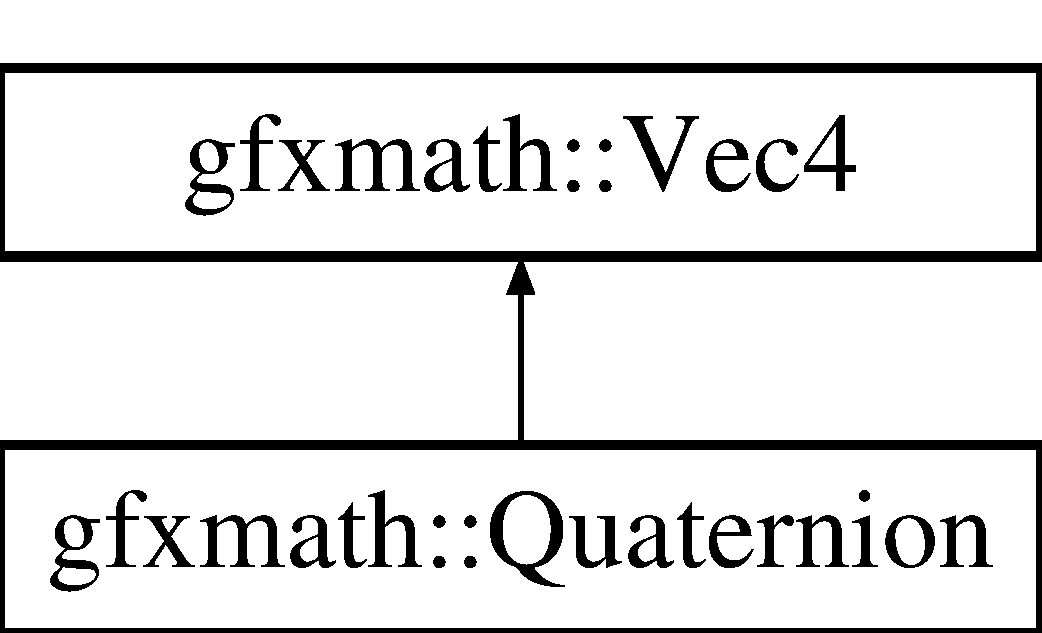
\includegraphics[height=2.000000cm]{classgfxmath_1_1_quaternion}
\end{center}
\end{figure}
\subsection*{Public Member Functions}
\begin{DoxyCompactItemize}
\item 
\hyperlink{classgfxmath_1_1_quaternion_a46f549f23e8bd1032697e3febcff7fe5}{Quaternion} ()
\begin{DoxyCompactList}\small\item\em Constructs a \hyperlink{classgfxmath_1_1_quaternion}{Quaternion} with all four components being initialized to 0.\+0f. \end{DoxyCompactList}\item 
\hyperlink{classgfxmath_1_1_quaternion_ac8a094f33b02273387afa1beeabb9034}{Quaternion} (float xyzw)
\begin{DoxyCompactList}\small\item\em Constructor taking a single float argument that will be copied into all four component values. \end{DoxyCompactList}\item 
\hyperlink{classgfxmath_1_1_quaternion_a8b19546f4e4a48a3784b80b0fd8208d9}{Quaternion} (float \hyperlink{classgfxmath_1_1_vec4_a273598aff75406f0e7a47121b8b06037}{x}, float \hyperlink{classgfxmath_1_1_vec4_a95e0ca27d66d7e0223606c20d326b595}{y}, float \hyperlink{classgfxmath_1_1_vec4_acd626b757468a5ea39f98812a36c4419}{z}, float \hyperlink{classgfxmath_1_1_vec4_adf2769a47b464dfee8d04e191f21701e}{w})
\begin{DoxyCompactList}\small\item\em Constructor taking four separate component values to use for the respective coordinate components of this \hyperlink{classgfxmath_1_1_quaternion}{Quaternion}. \end{DoxyCompactList}\item 
\hyperlink{classgfxmath_1_1_quaternion_a4034b6d18b58b65ecf329531d78317db}{Quaternion} (const \hyperlink{classgfxmath_1_1_vec2}{Vec2} \&xy, const \hyperlink{classgfxmath_1_1_vec2}{Vec2} \&zw)
\begin{DoxyCompactList}\small\item\em Constructor that takes two \hyperlink{classgfxmath_1_1_vec2}{Vec2} arguments and copies their values into the first and second pair of components, respectively. \end{DoxyCompactList}\item 
\hyperlink{classgfxmath_1_1_quaternion_a3ae6c4d2f305a7d89f517fdab000152b}{Quaternion} (const \hyperlink{classgfxmath_1_1_vec2}{Vec2} \&xy, float \hyperlink{classgfxmath_1_1_vec4_acd626b757468a5ea39f98812a36c4419}{z}, float \hyperlink{classgfxmath_1_1_vec4_adf2769a47b464dfee8d04e191f21701e}{w})
\begin{DoxyCompactList}\small\item\em Constructor taking a \hyperlink{classgfxmath_1_1_vec2}{Vec2} for the x and y-\/component values, then two separate floats for the z and w-\/coordinate component values. \end{DoxyCompactList}\item 
\hyperlink{classgfxmath_1_1_quaternion_a3c3a835a39e53ccdccd9b5cce341f379}{Quaternion} (float \hyperlink{classgfxmath_1_1_vec4_a273598aff75406f0e7a47121b8b06037}{x}, const \hyperlink{classgfxmath_1_1_vec2}{Vec2} \&yz, float \hyperlink{classgfxmath_1_1_vec4_adf2769a47b464dfee8d04e191f21701e}{w})
\begin{DoxyCompactList}\small\item\em Constructor taking a single float for the x-\/coordinate component, followed by a \hyperlink{classgfxmath_1_1_vec2}{Vec2} for the y and z-\/coordinate component values, then another floats for the w-\/coordinate component. \end{DoxyCompactList}\item 
\hyperlink{classgfxmath_1_1_quaternion_ae3fb1cfeffa2dfe7e5f798d79148eb99}{Quaternion} (float \hyperlink{classgfxmath_1_1_vec4_a273598aff75406f0e7a47121b8b06037}{x}, float \hyperlink{classgfxmath_1_1_vec4_a95e0ca27d66d7e0223606c20d326b595}{y}, const \hyperlink{classgfxmath_1_1_vec2}{Vec2} \&zw)
\begin{DoxyCompactList}\small\item\em Constructor taking two float values for the x and y-\/coordinate component values, followed by a \hyperlink{classgfxmath_1_1_vec2}{Vec2} for the z and w-\/coordinate component values. \end{DoxyCompactList}\item 
\hyperlink{classgfxmath_1_1_quaternion_a86f8a453d076124dc9d19f7e8ab9f045}{Quaternion} (const \hyperlink{classgfxmath_1_1_vec3}{Vec3} \&xyz, float \hyperlink{classgfxmath_1_1_vec4_adf2769a47b464dfee8d04e191f21701e}{w})
\begin{DoxyCompactList}\small\item\em Constructor taking a single \hyperlink{classgfxmath_1_1_vec3}{Vec3} for the x, y, and z-\/coordinate component values, followed by a single float for the w-\/coordinate component value. \end{DoxyCompactList}\item 
\hyperlink{classgfxmath_1_1_quaternion_aa91bb97300aa0a6058f0e7ebb52c04db}{Quaternion} (float \hyperlink{classgfxmath_1_1_vec4_a273598aff75406f0e7a47121b8b06037}{x}, const \hyperlink{classgfxmath_1_1_vec3}{Vec3} \&yzw)
\begin{DoxyCompactList}\small\item\em Constructor taking a single float for the w-\/coordinate component value, followed by a single \hyperlink{classgfxmath_1_1_vec3}{Vec3} for the x, y, and z-\/coordinate component values. \end{DoxyCompactList}\end{DoxyCompactItemize}
\subsection*{Static Public Attributes}
\begin{DoxyCompactItemize}
\item 
\hypertarget{classgfxmath_1_1_quaternion_a077623f1e442ee4a48340cc966282a1e}{}static const \hyperlink{classgfxmath_1_1_quaternion}{Quaternion} \hyperlink{classgfxmath_1_1_quaternion_a077623f1e442ee4a48340cc966282a1e}{I\+D\+E\+N\+T}\label{classgfxmath_1_1_quaternion_a077623f1e442ee4a48340cc966282a1e}

\begin{DoxyCompactList}\small\item\em The identity quaternion. \end{DoxyCompactList}\end{DoxyCompactItemize}
\subsection*{Related Functions}
(Note that these are not member functions.) {\bf }\par
\begin{DoxyCompactItemize}
\item 
\hyperlink{classgfxmath_1_1_quaternion}{Quaternion} \hyperlink{classgfxmath_1_1_quaternion_a0b4dfb2804fb5c44a112dc6b8ea43278}{Quaternion\+Normalize} (const \hyperlink{classgfxmath_1_1_quaternion}{Quaternion} \&quat)
\begin{DoxyCompactList}\small\item\em Normalize the given quaternion. \end{DoxyCompactList}\item 
\hyperlink{classgfxmath_1_1_quaternion}{Quaternion} \hyperlink{classgfxmath_1_1_quaternion_a01d5534572884ea932229ccb1aa17ac1}{Quaternion\+Multiply} (const \hyperlink{classgfxmath_1_1_quaternion}{Quaternion} \&q0, const \hyperlink{classgfxmath_1_1_quaternion}{Quaternion} \&q1)
\begin{DoxyCompactList}\small\item\em Multiply the two given Quaternions. \end{DoxyCompactList}\item 
\hyperlink{classgfxmath_1_1_quaternion}{Quaternion} \hyperlink{classgfxmath_1_1_quaternion_a7d4ad4615b2edcd99e9dcf6f0afe74ca}{Quaternion\+Lerp} (const \hyperlink{classgfxmath_1_1_quaternion}{Quaternion} \&q\+Start, const \hyperlink{classgfxmath_1_1_quaternion}{Quaternion} \&q\+End, float t)
\begin{DoxyCompactList}\small\item\em Linearly interpolate the given quaternions for time t. \end{DoxyCompactList}\item 
\hyperlink{classgfxmath_1_1_quaternion}{Quaternion} \hyperlink{classgfxmath_1_1_quaternion_abbc754cd1e171bd2d945376bb8a39a8f}{Quaternion\+From\+Axis\+Angle} (const \hyperlink{classgfxmath_1_1_vec3}{Vec3} \&axis\+Vec, float angle)
\begin{DoxyCompactList}\small\item\em Produces a quaternion representation of the given axis-\/angle rotation. \end{DoxyCompactList}\item 
\hyperlink{classgfxmath_1_1_quaternion}{Quaternion} \hyperlink{classgfxmath_1_1_quaternion_a6ea767e2a30159fd9c671ce16e949e38}{Quaternion\+From\+Euler} (const \hyperlink{classgfxmath_1_1_vec3}{Vec3} \&angles)
\begin{DoxyCompactList}\small\item\em Converts the given euler angles to a quaternion. \end{DoxyCompactList}\end{DoxyCompactItemize}

\subsection*{Additional Inherited Members}


\subsection{Detailed Description}
The quaternion class. 

\begin{DoxyDate}{Date}
2/21/2015
\end{DoxyDate}
\begin{DoxyRemark}{Remarks}
A specialized \hyperlink{classgfxmath_1_1_vec4}{Vec4} used to contain quaternion-\/based rotation data.
\end{DoxyRemark}
\begin{DoxySeeAlso}{See also}
\hyperlink{classgfxmath_1_1_vec4}{Vec4} 
\end{DoxySeeAlso}


\subsection{Constructor \& Destructor Documentation}
\hypertarget{classgfxmath_1_1_quaternion_a46f549f23e8bd1032697e3febcff7fe5}{}\index{gfxmath\+::\+Quaternion@{gfxmath\+::\+Quaternion}!Quaternion@{Quaternion}}
\index{Quaternion@{Quaternion}!gfxmath\+::\+Quaternion@{gfxmath\+::\+Quaternion}}
\subsubsection[{Quaternion}]{\setlength{\rightskip}{0pt plus 5cm}gfxmath\+::\+Quaternion\+::\+Quaternion (
\begin{DoxyParamCaption}
{}
\end{DoxyParamCaption}
)}\label{classgfxmath_1_1_quaternion_a46f549f23e8bd1032697e3febcff7fe5}


Constructs a \hyperlink{classgfxmath_1_1_quaternion}{Quaternion} with all four components being initialized to 0.\+0f. 

\begin{DoxyDate}{Date}
2/22/2015 
\end{DoxyDate}
\hypertarget{classgfxmath_1_1_quaternion_ac8a094f33b02273387afa1beeabb9034}{}\index{gfxmath\+::\+Quaternion@{gfxmath\+::\+Quaternion}!Quaternion@{Quaternion}}
\index{Quaternion@{Quaternion}!gfxmath\+::\+Quaternion@{gfxmath\+::\+Quaternion}}
\subsubsection[{Quaternion}]{\setlength{\rightskip}{0pt plus 5cm}gfxmath\+::\+Quaternion\+::\+Quaternion (
\begin{DoxyParamCaption}
\item[{float}]{xyzw}
\end{DoxyParamCaption}
)}\label{classgfxmath_1_1_quaternion_ac8a094f33b02273387afa1beeabb9034}


Constructor taking a single float argument that will be copied into all four component values. 

\begin{DoxyDate}{Date}
2/22/2015
\end{DoxyDate}

\begin{DoxyParams}{Parameters}
{\em xyzw} & The value that will be copied into the x, y, z, and w components. \\
\hline
\end{DoxyParams}
\hypertarget{classgfxmath_1_1_quaternion_a8b19546f4e4a48a3784b80b0fd8208d9}{}\index{gfxmath\+::\+Quaternion@{gfxmath\+::\+Quaternion}!Quaternion@{Quaternion}}
\index{Quaternion@{Quaternion}!gfxmath\+::\+Quaternion@{gfxmath\+::\+Quaternion}}
\subsubsection[{Quaternion}]{\setlength{\rightskip}{0pt plus 5cm}gfxmath\+::\+Quaternion\+::\+Quaternion (
\begin{DoxyParamCaption}
\item[{float}]{x, }
\item[{float}]{y, }
\item[{float}]{z, }
\item[{float}]{w}
\end{DoxyParamCaption}
)}\label{classgfxmath_1_1_quaternion_a8b19546f4e4a48a3784b80b0fd8208d9}


Constructor taking four separate component values to use for the respective coordinate components of this \hyperlink{classgfxmath_1_1_quaternion}{Quaternion}. 

\begin{DoxyDate}{Date}
2/22/2015
\end{DoxyDate}

\begin{DoxyParams}{Parameters}
{\em x} & The x-\/coordinate component value of this \hyperlink{classgfxmath_1_1_quaternion}{Quaternion}. \\
\hline
{\em y} & The y-\/coordinate component value of this \hyperlink{classgfxmath_1_1_quaternion}{Quaternion}. \\
\hline
{\em z} & The z-\/coordinate component value of this \hyperlink{classgfxmath_1_1_quaternion}{Quaternion}. \\
\hline
{\em w} & The w-\/coordinate component value of this \hyperlink{classgfxmath_1_1_quaternion}{Quaternion}. \\
\hline
\end{DoxyParams}
\hypertarget{classgfxmath_1_1_quaternion_a4034b6d18b58b65ecf329531d78317db}{}\index{gfxmath\+::\+Quaternion@{gfxmath\+::\+Quaternion}!Quaternion@{Quaternion}}
\index{Quaternion@{Quaternion}!gfxmath\+::\+Quaternion@{gfxmath\+::\+Quaternion}}
\subsubsection[{Quaternion}]{\setlength{\rightskip}{0pt plus 5cm}gfxmath\+::\+Quaternion\+::\+Quaternion (
\begin{DoxyParamCaption}
\item[{const {\bf Vec2} \&}]{xy, }
\item[{const {\bf Vec2} \&}]{zw}
\end{DoxyParamCaption}
)}\label{classgfxmath_1_1_quaternion_a4034b6d18b58b65ecf329531d78317db}


Constructor that takes two \hyperlink{classgfxmath_1_1_vec2}{Vec2} arguments and copies their values into the first and second pair of components, respectively. 

\begin{DoxyDate}{Date}
2/22/2015
\end{DoxyDate}

\begin{DoxyParams}{Parameters}
{\em xy} & The \hyperlink{classgfxmath_1_1_vec2}{Vec2} that will contribute its components to the x and y-\/coordinate components of this \hyperlink{classgfxmath_1_1_quaternion}{Quaternion}. \\
\hline
{\em zw} & The \hyperlink{classgfxmath_1_1_vec2}{Vec2} that will contribute its components to the z and w-\/coordinate components of this \hyperlink{classgfxmath_1_1_quaternion}{Quaternion}. \\
\hline
\end{DoxyParams}
\hypertarget{classgfxmath_1_1_quaternion_a3ae6c4d2f305a7d89f517fdab000152b}{}\index{gfxmath\+::\+Quaternion@{gfxmath\+::\+Quaternion}!Quaternion@{Quaternion}}
\index{Quaternion@{Quaternion}!gfxmath\+::\+Quaternion@{gfxmath\+::\+Quaternion}}
\subsubsection[{Quaternion}]{\setlength{\rightskip}{0pt plus 5cm}gfxmath\+::\+Quaternion\+::\+Quaternion (
\begin{DoxyParamCaption}
\item[{const {\bf Vec2} \&}]{xy, }
\item[{float}]{z, }
\item[{float}]{w}
\end{DoxyParamCaption}
)}\label{classgfxmath_1_1_quaternion_a3ae6c4d2f305a7d89f517fdab000152b}


Constructor taking a \hyperlink{classgfxmath_1_1_vec2}{Vec2} for the x and y-\/component values, then two separate floats for the z and w-\/coordinate component values. 

\begin{DoxyDate}{Date}
2/22/2015
\end{DoxyDate}

\begin{DoxyParams}{Parameters}
{\em xy} & The \hyperlink{classgfxmath_1_1_vec2}{Vec2} that will contribute its components to the x and y-\/coordinate components of this \hyperlink{classgfxmath_1_1_quaternion}{Quaternion}. \\
\hline
{\em z} & The z-\/coordinate component value of this \hyperlink{classgfxmath_1_1_quaternion}{Quaternion}. \\
\hline
{\em w} & The w-\/coordinate component value of this \hyperlink{classgfxmath_1_1_quaternion}{Quaternion}. \\
\hline
\end{DoxyParams}
\hypertarget{classgfxmath_1_1_quaternion_a3c3a835a39e53ccdccd9b5cce341f379}{}\index{gfxmath\+::\+Quaternion@{gfxmath\+::\+Quaternion}!Quaternion@{Quaternion}}
\index{Quaternion@{Quaternion}!gfxmath\+::\+Quaternion@{gfxmath\+::\+Quaternion}}
\subsubsection[{Quaternion}]{\setlength{\rightskip}{0pt plus 5cm}gfxmath\+::\+Quaternion\+::\+Quaternion (
\begin{DoxyParamCaption}
\item[{float}]{x, }
\item[{const {\bf Vec2} \&}]{yz, }
\item[{float}]{w}
\end{DoxyParamCaption}
)}\label{classgfxmath_1_1_quaternion_a3c3a835a39e53ccdccd9b5cce341f379}


Constructor taking a single float for the x-\/coordinate component, followed by a \hyperlink{classgfxmath_1_1_vec2}{Vec2} for the y and z-\/coordinate component values, then another floats for the w-\/coordinate component. 

\begin{DoxyDate}{Date}
2/22/2015
\end{DoxyDate}

\begin{DoxyParams}{Parameters}
{\em x} & The x-\/coordinate component value of this \hyperlink{classgfxmath_1_1_quaternion}{Quaternion}. \\
\hline
{\em yz} & The \hyperlink{classgfxmath_1_1_vec2}{Vec2} that will contribute its components to the y and z-\/coordinate components of this \hyperlink{classgfxmath_1_1_quaternion}{Quaternion}. \\
\hline
{\em w} & The w-\/coordinate component value of this \hyperlink{classgfxmath_1_1_quaternion}{Quaternion}. \\
\hline
\end{DoxyParams}
\hypertarget{classgfxmath_1_1_quaternion_ae3fb1cfeffa2dfe7e5f798d79148eb99}{}\index{gfxmath\+::\+Quaternion@{gfxmath\+::\+Quaternion}!Quaternion@{Quaternion}}
\index{Quaternion@{Quaternion}!gfxmath\+::\+Quaternion@{gfxmath\+::\+Quaternion}}
\subsubsection[{Quaternion}]{\setlength{\rightskip}{0pt plus 5cm}gfxmath\+::\+Quaternion\+::\+Quaternion (
\begin{DoxyParamCaption}
\item[{float}]{x, }
\item[{float}]{y, }
\item[{const {\bf Vec2} \&}]{zw}
\end{DoxyParamCaption}
)}\label{classgfxmath_1_1_quaternion_ae3fb1cfeffa2dfe7e5f798d79148eb99}


Constructor taking two float values for the x and y-\/coordinate component values, followed by a \hyperlink{classgfxmath_1_1_vec2}{Vec2} for the z and w-\/coordinate component values. 

\begin{DoxyDate}{Date}
2/22/2015
\end{DoxyDate}

\begin{DoxyParams}{Parameters}
{\em x} & The x-\/coordinate component value of this \hyperlink{classgfxmath_1_1_quaternion}{Quaternion}. \\
\hline
{\em y} & The y-\/coordinate component value of this \hyperlink{classgfxmath_1_1_quaternion}{Quaternion}. \\
\hline
{\em zw} & The \hyperlink{classgfxmath_1_1_vec2}{Vec2} that will contribute its components to the z and w-\/coordinate components of this \hyperlink{classgfxmath_1_1_quaternion}{Quaternion}. \\
\hline
\end{DoxyParams}
\hypertarget{classgfxmath_1_1_quaternion_a86f8a453d076124dc9d19f7e8ab9f045}{}\index{gfxmath\+::\+Quaternion@{gfxmath\+::\+Quaternion}!Quaternion@{Quaternion}}
\index{Quaternion@{Quaternion}!gfxmath\+::\+Quaternion@{gfxmath\+::\+Quaternion}}
\subsubsection[{Quaternion}]{\setlength{\rightskip}{0pt plus 5cm}gfxmath\+::\+Quaternion\+::\+Quaternion (
\begin{DoxyParamCaption}
\item[{const {\bf Vec3} \&}]{xyz, }
\item[{float}]{w}
\end{DoxyParamCaption}
)}\label{classgfxmath_1_1_quaternion_a86f8a453d076124dc9d19f7e8ab9f045}


Constructor taking a single \hyperlink{classgfxmath_1_1_vec3}{Vec3} for the x, y, and z-\/coordinate component values, followed by a single float for the w-\/coordinate component value. 

\begin{DoxyDate}{Date}
2/22/2015
\end{DoxyDate}

\begin{DoxyParams}{Parameters}
{\em xyz} & The \hyperlink{classgfxmath_1_1_vec3}{Vec3} that will contribute its components to the x, y and z-\/coordinate components of this \hyperlink{classgfxmath_1_1_quaternion}{Quaternion}. \\
\hline
{\em w} & The w-\/coordinate component value of this \hyperlink{classgfxmath_1_1_quaternion}{Quaternion}. \\
\hline
\end{DoxyParams}
\hypertarget{classgfxmath_1_1_quaternion_aa91bb97300aa0a6058f0e7ebb52c04db}{}\index{gfxmath\+::\+Quaternion@{gfxmath\+::\+Quaternion}!Quaternion@{Quaternion}}
\index{Quaternion@{Quaternion}!gfxmath\+::\+Quaternion@{gfxmath\+::\+Quaternion}}
\subsubsection[{Quaternion}]{\setlength{\rightskip}{0pt plus 5cm}gfxmath\+::\+Quaternion\+::\+Quaternion (
\begin{DoxyParamCaption}
\item[{float}]{x, }
\item[{const {\bf Vec3} \&}]{yzw}
\end{DoxyParamCaption}
)}\label{classgfxmath_1_1_quaternion_aa91bb97300aa0a6058f0e7ebb52c04db}


Constructor taking a single float for the w-\/coordinate component value, followed by a single \hyperlink{classgfxmath_1_1_vec3}{Vec3} for the x, y, and z-\/coordinate component values. 

\begin{DoxyDate}{Date}
2/22/2015
\end{DoxyDate}

\begin{DoxyParams}{Parameters}
{\em x} & The x-\/coordinate component value of this \hyperlink{classgfxmath_1_1_quaternion}{Quaternion}. \\
\hline
{\em yzw} & The \hyperlink{classgfxmath_1_1_vec3}{Vec3} that will contribute its components to the y, z and w-\/coordinate components of this \hyperlink{classgfxmath_1_1_quaternion}{Quaternion}. \\
\hline
\end{DoxyParams}


\subsection{Friends And Related Function Documentation}
\hypertarget{classgfxmath_1_1_quaternion_abbc754cd1e171bd2d945376bb8a39a8f}{}\index{gfxmath\+::\+Quaternion@{gfxmath\+::\+Quaternion}!Quaternion\+From\+Axis\+Angle@{Quaternion\+From\+Axis\+Angle}}
\index{Quaternion\+From\+Axis\+Angle@{Quaternion\+From\+Axis\+Angle}!gfxmath\+::\+Quaternion@{gfxmath\+::\+Quaternion}}
\subsubsection[{Quaternion\+From\+Axis\+Angle}]{\setlength{\rightskip}{0pt plus 5cm}{\bf Quaternion} Quaternion\+From\+Axis\+Angle (
\begin{DoxyParamCaption}
\item[{const {\bf Vec3} \&}]{axis\+Vec, }
\item[{float}]{angle}
\end{DoxyParamCaption}
)\hspace{0.3cm}{\ttfamily [related]}}\label{classgfxmath_1_1_quaternion_abbc754cd1e171bd2d945376bb8a39a8f}


Produces a quaternion representation of the given axis-\/angle rotation. 

\begin{DoxyDate}{Date}
2/22/2015
\end{DoxyDate}

\begin{DoxyParams}{Parameters}
{\em axis\+Vec} & The axis vec. \\
\hline
{\em angle} & The angle.\\
\hline
\end{DoxyParams}
\begin{DoxyReturn}{Returns}
The quaternion representation of the given axis-\/angle rotation. 
\end{DoxyReturn}
\hypertarget{classgfxmath_1_1_quaternion_a6ea767e2a30159fd9c671ce16e949e38}{}\index{gfxmath\+::\+Quaternion@{gfxmath\+::\+Quaternion}!Quaternion\+From\+Euler@{Quaternion\+From\+Euler}}
\index{Quaternion\+From\+Euler@{Quaternion\+From\+Euler}!gfxmath\+::\+Quaternion@{gfxmath\+::\+Quaternion}}
\subsubsection[{Quaternion\+From\+Euler}]{\setlength{\rightskip}{0pt plus 5cm}{\bf Quaternion} Quaternion\+From\+Euler (
\begin{DoxyParamCaption}
\item[{const {\bf Vec3} \&}]{angles}
\end{DoxyParamCaption}
)\hspace{0.3cm}{\ttfamily [related]}}\label{classgfxmath_1_1_quaternion_a6ea767e2a30159fd9c671ce16e949e38}


Converts the given euler angles to a quaternion. 

\begin{DoxyDate}{Date}
2/22/2015
\end{DoxyDate}

\begin{DoxyParams}{Parameters}
{\em angles} & The angles (in radians).\\
\hline
\end{DoxyParams}
\begin{DoxyReturn}{Returns}
A quaternion representing the given euler angles. 
\end{DoxyReturn}
\hypertarget{classgfxmath_1_1_quaternion_a7d4ad4615b2edcd99e9dcf6f0afe74ca}{}\index{gfxmath\+::\+Quaternion@{gfxmath\+::\+Quaternion}!Quaternion\+Lerp@{Quaternion\+Lerp}}
\index{Quaternion\+Lerp@{Quaternion\+Lerp}!gfxmath\+::\+Quaternion@{gfxmath\+::\+Quaternion}}
\subsubsection[{Quaternion\+Lerp}]{\setlength{\rightskip}{0pt plus 5cm}{\bf Quaternion} Quaternion\+Lerp (
\begin{DoxyParamCaption}
\item[{const {\bf Quaternion} \&}]{q\+Start, }
\item[{const {\bf Quaternion} \&}]{q\+End, }
\item[{float}]{t}
\end{DoxyParamCaption}
)\hspace{0.3cm}{\ttfamily [related]}}\label{classgfxmath_1_1_quaternion_a7d4ad4615b2edcd99e9dcf6f0afe74ca}


Linearly interpolate the given quaternions for time t. 

\begin{DoxyDate}{Date}
2/22/2015
\end{DoxyDate}

\begin{DoxyParams}{Parameters}
{\em q\+Start} & The start quaternion. \\
\hline
{\em q\+End} & The end quaternion. \\
\hline
{\em t} & The \char`\"{}time\char`\"{} between the two quaternions.\\
\hline
\end{DoxyParams}
\begin{DoxyReturn}{Returns}
The quaternion lerped between q\+Start and q\+End at time \textquotesingle{}t\textquotesingle{}. 
\end{DoxyReturn}
\hypertarget{classgfxmath_1_1_quaternion_a01d5534572884ea932229ccb1aa17ac1}{}\index{gfxmath\+::\+Quaternion@{gfxmath\+::\+Quaternion}!Quaternion\+Multiply@{Quaternion\+Multiply}}
\index{Quaternion\+Multiply@{Quaternion\+Multiply}!gfxmath\+::\+Quaternion@{gfxmath\+::\+Quaternion}}
\subsubsection[{Quaternion\+Multiply}]{\setlength{\rightskip}{0pt plus 5cm}{\bf Quaternion} Quaternion\+Multiply (
\begin{DoxyParamCaption}
\item[{const {\bf Quaternion} \&}]{q0, }
\item[{const {\bf Quaternion} \&}]{q1}
\end{DoxyParamCaption}
)\hspace{0.3cm}{\ttfamily [related]}}\label{classgfxmath_1_1_quaternion_a01d5534572884ea932229ccb1aa17ac1}


Multiply the two given Quaternions. 

\begin{DoxyDate}{Date}
2/22/2015
\end{DoxyDate}

\begin{DoxyParams}{Parameters}
{\em q0} & The first quaternion in the multiplication. \\
\hline
{\em q1} & The second quaternion in the multiplication.\\
\hline
\end{DoxyParams}
\begin{DoxyReturn}{Returns}
The product of the two given quaternions. 
\end{DoxyReturn}
\hypertarget{classgfxmath_1_1_quaternion_a0b4dfb2804fb5c44a112dc6b8ea43278}{}\index{gfxmath\+::\+Quaternion@{gfxmath\+::\+Quaternion}!Quaternion\+Normalize@{Quaternion\+Normalize}}
\index{Quaternion\+Normalize@{Quaternion\+Normalize}!gfxmath\+::\+Quaternion@{gfxmath\+::\+Quaternion}}
\subsubsection[{Quaternion\+Normalize}]{\setlength{\rightskip}{0pt plus 5cm}{\bf Quaternion} Quaternion\+Normalize (
\begin{DoxyParamCaption}
\item[{const {\bf Quaternion} \&}]{quat}
\end{DoxyParamCaption}
)\hspace{0.3cm}{\ttfamily [related]}}\label{classgfxmath_1_1_quaternion_a0b4dfb2804fb5c44a112dc6b8ea43278}


Normalize the given quaternion. 

\begin{DoxyDate}{Date}
2/22/2015
\end{DoxyDate}

\begin{DoxyParams}{Parameters}
{\em quat} & The quaternion.\\
\hline
\end{DoxyParams}
\begin{DoxyReturn}{Returns}
A \hyperlink{classgfxmath_1_1_quaternion}{Quaternion}.
\end{DoxyReturn}
\begin{DoxyRemark}{Remarks}
Scales the components of the \hyperlink{classgfxmath_1_1_quaternion}{Quaternion} such that its length is 1 (unit length). 
\end{DoxyRemark}


The documentation for this class was generated from the following files\+:\begin{DoxyCompactItemize}
\item 
\hyperlink{quaternion_8h}{quaternion.\+h}\item 
\hyperlink{vecmath_8h}{vecmath.\+h}\end{DoxyCompactItemize}

\hypertarget{classgfxmath_1_1_sse_mat44}{}\section{gfxmath\+:\+:Sse\+Mat44 Class Reference}
\label{classgfxmath_1_1_sse_mat44}\index{gfxmath\+::\+Sse\+Mat44@{gfxmath\+::\+Sse\+Mat44}}


A 4x4 column-\/major matrix that uses four Sse\+Vecs for column vectors.  




{\ttfamily \#include $<$ssemat44.\+h$>$}

\subsection*{Public Member Functions}
\begin{DoxyCompactItemize}
\item 
\hyperlink{classgfxmath_1_1_sse_mat44_aeee33533bcfdba675609d5b1155cf029}{Sse\+Mat44} ()
\begin{DoxyCompactList}\small\item\em Empty \hyperlink{classgfxmath_1_1_sse_mat44}{Sse\+Mat44} constructor. \end{DoxyCompactList}\item 
\hyperlink{classgfxmath_1_1_sse_mat44_a60f6b91adfec4810007c8bef96bca42c}{Sse\+Mat44} (const \hyperlink{namespacegfxmath_a0de2243e2b8d0fd46d3af5e036423004}{Sse\+Vec} \&v0, const \hyperlink{namespacegfxmath_a0de2243e2b8d0fd46d3af5e036423004}{Sse\+Vec} \&v1, const \hyperlink{namespacegfxmath_a0de2243e2b8d0fd46d3af5e036423004}{Sse\+Vec} \&v2, const \hyperlink{namespacegfxmath_a0de2243e2b8d0fd46d3af5e036423004}{Sse\+Vec} \&v3, \hyperlink{group___s_i_s_d_mat_math_ga6c8951c82aec5015dd6806affb4c8d03}{Matrix\+Type} \hyperlink{classgfxmath_1_1_sse_mat44_abdcc4efbf8375bae103da12c0823a85c}{matrix\+Type\+Val}=Matrix\+Type\+::\+M\+I\+S\+C)
\begin{DoxyCompactList}\small\item\em \hyperlink{classgfxmath_1_1_sse_mat44}{Sse\+Mat44} constructor that takes Sse\+Vec arguments to fill the columns, and an optional Matrix\+Type argument to initialize its state. \end{DoxyCompactList}\item 
\hyperlink{classgfxmath_1_1_sse_mat44_a2fe0899f1f7a864586c5fb01397da259}{Sse\+Mat44} (const \hyperlink{classgfxmath_1_1_vec4}{Vec4} \&col0\+Param, const \hyperlink{classgfxmath_1_1_vec4}{Vec4} \&col1\+Param, const \hyperlink{classgfxmath_1_1_vec4}{Vec4} \&col2\+Param, const \hyperlink{classgfxmath_1_1_vec4}{Vec4} \&col3\+Param, \hyperlink{group___s_i_s_d_mat_math_ga6c8951c82aec5015dd6806affb4c8d03}{Matrix\+Type} \hyperlink{classgfxmath_1_1_sse_mat44_abdcc4efbf8375bae103da12c0823a85c}{matrix\+Type\+Val}=Matrix\+Type\+::\+M\+I\+S\+C)
\begin{DoxyCompactList}\small\item\em \hyperlink{classgfxmath_1_1_sse_mat44}{Sse\+Mat44} constructor that takes \hyperlink{classgfxmath_1_1_vec4}{Vec4} arguments to fill the columns, and an optional Matrix\+Type argument to initialize its state. \end{DoxyCompactList}\item 
\hyperlink{classgfxmath_1_1_sse_mat44_ae77c1fcd0efebbcea2cbc61b8849cbd4}{Sse\+Mat44} (float f00, float f10, float f20, float f30, float f01, float f11, float f21, float f31, float f02, float f12, float f22, float f32, float f03, float f13, float f23, float f33, \hyperlink{group___s_i_s_d_mat_math_ga6c8951c82aec5015dd6806affb4c8d03}{Matrix\+Type} \hyperlink{classgfxmath_1_1_sse_mat44_abdcc4efbf8375bae103da12c0823a85c}{matrix\+Type\+Val}=Matrix\+Type\+::\+M\+I\+S\+C)
\begin{DoxyCompactList}\small\item\em An \hyperlink{classgfxmath_1_1_sse_mat44}{Sse\+Mat44} constructor that takes 16 floats. \end{DoxyCompactList}\item 
\hyperlink{classgfxmath_1_1_sse_mat44_ae7f7bd62ac0d4d625a7b1d2701e8621f}{Sse\+Mat44} (\hyperlink{classgfxmath_1_1_mat44}{Mat44} \&mat)
\begin{DoxyCompactList}\small\item\em A conversion constructor from \hyperlink{classgfxmath_1_1_mat44}{Mat44} to \hyperlink{classgfxmath_1_1_sse_mat44}{Sse\+Mat44}. \end{DoxyCompactList}\end{DoxyCompactItemize}
\subsection*{Public Attributes}
\begin{DoxyCompactItemize}
\item 
\hyperlink{group___s_i_s_d_mat_math_ga6c8951c82aec5015dd6806affb4c8d03}{Matrix\+Type} \hyperlink{classgfxmath_1_1_sse_mat44_abdcc4efbf8375bae103da12c0823a85c}{matrix\+Type\+Val}
\begin{DoxyCompactList}\small\item\em A Matrix\+Type used to track the matrix state. \end{DoxyCompactList}\item 
\hyperlink{namespacegfxmath_a0de2243e2b8d0fd46d3af5e036423004}{Sse\+Vec} \hyperlink{classgfxmath_1_1_sse_mat44_a5ba91c42ffa3a8158266badf214b07a6}{col0}
\begin{DoxyCompactList}\small\item\em The first column vector. \end{DoxyCompactList}\item 
\hyperlink{namespacegfxmath_a0de2243e2b8d0fd46d3af5e036423004}{Sse\+Vec} \hyperlink{classgfxmath_1_1_sse_mat44_a836c79e6497a5aa122c240767e7376a1}{col1}
\begin{DoxyCompactList}\small\item\em The second column vector. \end{DoxyCompactList}\item 
\hyperlink{namespacegfxmath_a0de2243e2b8d0fd46d3af5e036423004}{Sse\+Vec} \hyperlink{classgfxmath_1_1_sse_mat44_a636928a37222e474300ea4aa5ff5221c}{col2}
\begin{DoxyCompactList}\small\item\em The third column vector. \end{DoxyCompactList}\item 
\hyperlink{namespacegfxmath_a0de2243e2b8d0fd46d3af5e036423004}{Sse\+Vec} \hyperlink{classgfxmath_1_1_sse_mat44_a7ee53ec82e31166ee87c6dfe6bc5810c}{col3}
\begin{DoxyCompactList}\small\item\em The fourth column vector. \end{DoxyCompactList}\end{DoxyCompactItemize}
\subsection*{Static Public Attributes}
\begin{DoxyCompactItemize}
\item 
\hypertarget{classgfxmath_1_1_sse_mat44_a1da166cfaf4bd0082c0a6ee1c62153a1}{}static const \hyperlink{classgfxmath_1_1_sse_mat44}{Sse\+Mat44} \hyperlink{classgfxmath_1_1_sse_mat44_a1da166cfaf4bd0082c0a6ee1c62153a1}{I\+D\+E\+N\+T\+I\+T\+Y}\label{classgfxmath_1_1_sse_mat44_a1da166cfaf4bd0082c0a6ee1c62153a1}

\begin{DoxyCompactList}\small\item\em The identity matrix. \end{DoxyCompactList}\end{DoxyCompactItemize}
\subsection*{Related Functions}
(Note that these are not member functions.) {\bf }\par
\begin{DoxyCompactItemize}
\item 
std\+::array$<$ float, 16 $>$ \hyperlink{classgfxmath_1_1_sse_mat44_a5f87ab4eb6093d145cda3e6772c6bc0a}{Matrix\+To\+Array} (const \hyperlink{classgfxmath_1_1_sse_mat44}{Sse\+Mat44} \&mat)
\begin{DoxyCompactList}\small\item\em Converts the given 4x4 matrix to an array of floats. \end{DoxyCompactList}\item 
\hyperlink{ssemat__math__defs_8h_a741f88d5589197d03fea9ab2b7622b8a}{S\+S\+E\+\_\+\+M\+A\+T\+\_\+\+C\+A\+L\+L} \hyperlink{classgfxmath_1_1_sse_mat44_ab38872b965a424d2660e1c4be71ddbe6}{Matrix\+Multiply} (const \hyperlink{classgfxmath_1_1_sse_mat44}{Sse\+Mat44} \&left, const \hyperlink{classgfxmath_1_1_sse_mat44}{Sse\+Mat44} \&right)
\begin{DoxyCompactList}\small\item\em Calculates the product (post-\/multiplication) of the two given 4x4 matrices. \end{DoxyCompactList}\item 
\hyperlink{ssemat__math__defs_8h_a741f88d5589197d03fea9ab2b7622b8a}{S\+S\+E\+\_\+\+M\+A\+T\+\_\+\+C\+A\+L\+L} \hyperlink{classgfxmath_1_1_sse_mat44_a7d63a634b20c220ad6047dc4633bf70f}{Matrix\+Inverse} (const \hyperlink{classgfxmath_1_1_sse_mat44}{Sse\+Mat44} \&mat)
\begin{DoxyCompactList}\small\item\em Calculates the inverse of the given 4x4 matrix. \end{DoxyCompactList}\item 
\hyperlink{ssemat__math__defs_8h_a741f88d5589197d03fea9ab2b7622b8a}{S\+S\+E\+\_\+\+M\+A\+T\+\_\+\+C\+A\+L\+L} \hyperlink{classgfxmath_1_1_sse_mat44_a8c2545c52a86496bdf8917a1158f6f24}{Matrix\+Transpose} (const \hyperlink{classgfxmath_1_1_sse_mat44}{Sse\+Mat44} \&mat)
\begin{DoxyCompactList}\small\item\em Calculates the transpose of the given 4x4 matrix. \end{DoxyCompactList}\item 
\hyperlink{namespacegfxmath_a0de2243e2b8d0fd46d3af5e036423004}{Sse\+Vec} \hyperlink{classgfxmath_1_1_sse_mat44_a6709364ddedc83299a1d6a58607a87aa}{Matrix\+Determinant} (const \hyperlink{classgfxmath_1_1_sse_mat44}{Sse\+Mat44} \&mat)
\begin{DoxyCompactList}\small\item\em Calculates the determinant of the given \hyperlink{classgfxmath_1_1_sse_mat44}{Sse\+Mat44}. \end{DoxyCompactList}\item 
\hyperlink{ssemat__math__defs_8h_a741f88d5589197d03fea9ab2b7622b8a}{S\+S\+E\+\_\+\+M\+A\+T\+\_\+\+C\+A\+L\+L} \hyperlink{classgfxmath_1_1_sse_mat44_a786ee918eca59978387d6fce4dab5122}{Rotation\+Matrix\+From\+Quaternion} (const \hyperlink{namespacegfxmath_a0de2243e2b8d0fd46d3af5e036423004}{Sse\+Vec} \&quat)
\begin{DoxyCompactList}\small\item\em Calculates the 4x4 rotation matrix represented by the given quaternion rotation. \end{DoxyCompactList}\item 
\hyperlink{ssemat__math__defs_8h_a741f88d5589197d03fea9ab2b7622b8a}{S\+S\+E\+\_\+\+M\+A\+T\+\_\+\+C\+A\+L\+L} \hyperlink{classgfxmath_1_1_sse_mat44_ac11c40e17108aa72d069b01b6a08bebf}{Rotation\+Matrix\+From\+Euler} (const \hyperlink{namespacegfxmath_a0de2243e2b8d0fd46d3af5e036423004}{Sse\+Vec} \&angles)
\begin{DoxyCompactList}\small\item\em Calculates the 4x4 rotation matrix represented by the given euler angle rotation. \end{DoxyCompactList}\item 
\hyperlink{ssemat__math__defs_8h_a741f88d5589197d03fea9ab2b7622b8a}{S\+S\+E\+\_\+\+M\+A\+T\+\_\+\+C\+A\+L\+L} \hyperlink{classgfxmath_1_1_sse_mat44_a2b08e7c142f14df78883494d9c2f66e8}{Translation\+Matrix\+From\+Vec3} (const \hyperlink{namespacegfxmath_a0de2243e2b8d0fd46d3af5e036423004}{Sse\+Vec} \&vec)
\begin{DoxyCompactList}\small\item\em Calculates the 4x4 translation matrix represented by the given 3\+D position vector. \end{DoxyCompactList}\item 
\hyperlink{ssemat__math__defs_8h_a741f88d5589197d03fea9ab2b7622b8a}{S\+S\+E\+\_\+\+M\+A\+T\+\_\+\+C\+A\+L\+L} \hyperlink{classgfxmath_1_1_sse_mat44_a7971ccb3a66b526ba72c66477539c923}{Scale\+Matrix\+From\+Vec3} (const \hyperlink{namespacegfxmath_a0de2243e2b8d0fd46d3af5e036423004}{Sse\+Vec} \&vec)
\begin{DoxyCompactList}\small\item\em Calculates the 4x4 scale matrix represented by the given 3\+D scale vector. \end{DoxyCompactList}\item 
\hyperlink{ssemat__math__defs_8h_a741f88d5589197d03fea9ab2b7622b8a}{S\+S\+E\+\_\+\+M\+A\+T\+\_\+\+C\+A\+L\+L} \hyperlink{classgfxmath_1_1_sse_mat44_a701f5bfeb4c0c0d4b080a9ad00f910ce}{Perspective\+Projection\+Matrix} (float near, float far, float fov, float aspect)
\begin{DoxyCompactList}\small\item\em Calculates the right-\/handed perspective projection matrix. \end{DoxyCompactList}\item 
\hyperlink{ssemat__math__defs_8h_a741f88d5589197d03fea9ab2b7622b8a}{S\+S\+E\+\_\+\+M\+A\+T\+\_\+\+C\+A\+L\+L} \hyperlink{classgfxmath_1_1_sse_mat44_a67dc21f3890ac0ef9a36b05b71ad36db}{Look\+Dir} (const \hyperlink{namespacegfxmath_a0de2243e2b8d0fd46d3af5e036423004}{Sse\+Vec} \&eye, const \hyperlink{namespacegfxmath_a0de2243e2b8d0fd46d3af5e036423004}{Sse\+Vec} \&dir, const \hyperlink{namespacegfxmath_a0de2243e2b8d0fd46d3af5e036423004}{Sse\+Vec} \&up)
\begin{DoxyCompactList}\small\item\em Calculates the view matrix given the forward direction vector, rather than a target position. \end{DoxyCompactList}\item 
\hyperlink{ssemat__math__defs_8h_a741f88d5589197d03fea9ab2b7622b8a}{S\+S\+E\+\_\+\+M\+A\+T\+\_\+\+C\+A\+L\+L} \hyperlink{classgfxmath_1_1_sse_mat44_abc7554e34178f4e36a906a12ea469c64}{Look\+At} (const \hyperlink{namespacegfxmath_a0de2243e2b8d0fd46d3af5e036423004}{Sse\+Vec} \&eye, const \hyperlink{namespacegfxmath_a0de2243e2b8d0fd46d3af5e036423004}{Sse\+Vec} \&target, const \hyperlink{namespacegfxmath_a0de2243e2b8d0fd46d3af5e036423004}{Sse\+Vec} \&up)
\begin{DoxyCompactList}\small\item\em Calculates the standard lookat matrix for the camera, given the camera\textquotesingle{}s position, the target\textquotesingle{}s position, and a given \char`\"{}up\char`\"{} vector. \end{DoxyCompactList}\item 
\hyperlink{namespacegfxmath_a0de2243e2b8d0fd46d3af5e036423004}{Sse\+Vec} \hyperlink{classgfxmath_1_1_sse_mat44_a7f0f017f89ae1ba6cf642fba6ce8e4cd}{Transform\+Vec3} (const \hyperlink{classgfxmath_1_1_sse_mat44}{Sse\+Mat44} \&mat, const \hyperlink{namespacegfxmath_a0de2243e2b8d0fd46d3af5e036423004}{Sse\+Vec} \&vec)
\begin{DoxyCompactList}\small\item\em Transforms the given 3\+D vector via the given \hyperlink{classgfxmath_1_1_sse_mat44}{Sse\+Mat44} matrix. \end{DoxyCompactList}\end{DoxyCompactItemize}



\subsection{Detailed Description}
A 4x4 column-\/major matrix that uses four Sse\+Vecs for column vectors. 

\begin{DoxyReturn}{Returns}
The S\+S\+E matrix 44.
\end{DoxyReturn}
\begin{DoxyRemark}{Remarks}
This class is used to take advantage of sse intrinsics for substantial performance gains in cpu-\/heavy rendering calculations. 
\end{DoxyRemark}


\subsection{Constructor \& Destructor Documentation}
\hypertarget{classgfxmath_1_1_sse_mat44_aeee33533bcfdba675609d5b1155cf029}{}\index{gfxmath\+::\+Sse\+Mat44@{gfxmath\+::\+Sse\+Mat44}!Sse\+Mat44@{Sse\+Mat44}}
\index{Sse\+Mat44@{Sse\+Mat44}!gfxmath\+::\+Sse\+Mat44@{gfxmath\+::\+Sse\+Mat44}}
\subsubsection[{Sse\+Mat44}]{\setlength{\rightskip}{0pt plus 5cm}gfxmath\+::\+Sse\+Mat44\+::\+Sse\+Mat44 (
\begin{DoxyParamCaption}
{}
\end{DoxyParamCaption}
)\hspace{0.3cm}{\ttfamily [inline]}}\label{classgfxmath_1_1_sse_mat44_aeee33533bcfdba675609d5b1155cf029}


Empty \hyperlink{classgfxmath_1_1_sse_mat44}{Sse\+Mat44} constructor. 

\begin{DoxyDate}{Date}
2/21/2015
\end{DoxyDate}
\begin{DoxyRemark}{Remarks}
Sets all member columns to zerovectors, and sets the matrix\+Type\+Val to Matrix\+Type\+::\+M\+I\+S\+C. 
\end{DoxyRemark}
\hypertarget{classgfxmath_1_1_sse_mat44_a60f6b91adfec4810007c8bef96bca42c}{}\index{gfxmath\+::\+Sse\+Mat44@{gfxmath\+::\+Sse\+Mat44}!Sse\+Mat44@{Sse\+Mat44}}
\index{Sse\+Mat44@{Sse\+Mat44}!gfxmath\+::\+Sse\+Mat44@{gfxmath\+::\+Sse\+Mat44}}
\subsubsection[{Sse\+Mat44}]{\setlength{\rightskip}{0pt plus 5cm}gfxmath\+::\+Sse\+Mat44\+::\+Sse\+Mat44 (
\begin{DoxyParamCaption}
\item[{const {\bf Sse\+Vec} \&}]{v0, }
\item[{const {\bf Sse\+Vec} \&}]{v1, }
\item[{const {\bf Sse\+Vec} \&}]{v2, }
\item[{const {\bf Sse\+Vec} \&}]{v3, }
\item[{{\bf Matrix\+Type}}]{matrix\+Type\+Val = {\ttfamily MatrixType\+:\+:MISC}}
\end{DoxyParamCaption}
)\hspace{0.3cm}{\ttfamily [inline]}}\label{classgfxmath_1_1_sse_mat44_a60f6b91adfec4810007c8bef96bca42c}


\hyperlink{classgfxmath_1_1_sse_mat44}{Sse\+Mat44} constructor that takes Sse\+Vec arguments to fill the columns, and an optional Matrix\+Type argument to initialize its state. 

\begin{DoxyDate}{Date}
2/21/2015
\end{DoxyDate}

\begin{DoxyParams}{Parameters}
{\em v0} & An Sse\+Vec that will be placed in the first column. \\
\hline
{\em v1} & An Sse\+Vec that will be placed in the second column. \\
\hline
{\em v2} & An Sse\+Vec that will be placed in the third column. \\
\hline
{\em v3} & An Sse\+Vec that will be placed in the fourth column. \\
\hline
{\em matrix\+Type\+Val} & The matrix type value. Defaults as Matrix\+Type\+::\+M\+I\+S\+C\\
\hline
\end{DoxyParams}
\begin{DoxyRemark}{Remarks}
Sets its respective column vectors to the given Sse\+Vec arguments, and optionally sets the matrix\+Type\+Val to the given Matrix\+Type (defaults to Matrix\+Type\+::\+M\+I\+S\+C) 
\end{DoxyRemark}
\hypertarget{classgfxmath_1_1_sse_mat44_a2fe0899f1f7a864586c5fb01397da259}{}\index{gfxmath\+::\+Sse\+Mat44@{gfxmath\+::\+Sse\+Mat44}!Sse\+Mat44@{Sse\+Mat44}}
\index{Sse\+Mat44@{Sse\+Mat44}!gfxmath\+::\+Sse\+Mat44@{gfxmath\+::\+Sse\+Mat44}}
\subsubsection[{Sse\+Mat44}]{\setlength{\rightskip}{0pt plus 5cm}gfxmath\+::\+Sse\+Mat44\+::\+Sse\+Mat44 (
\begin{DoxyParamCaption}
\item[{const {\bf Vec4} \&}]{col0\+Param, }
\item[{const {\bf Vec4} \&}]{col1\+Param, }
\item[{const {\bf Vec4} \&}]{col2\+Param, }
\item[{const {\bf Vec4} \&}]{col3\+Param, }
\item[{{\bf Matrix\+Type}}]{matrix\+Type\+Val = {\ttfamily MatrixType\+:\+:MISC}}
\end{DoxyParamCaption}
)\hspace{0.3cm}{\ttfamily [inline]}}\label{classgfxmath_1_1_sse_mat44_a2fe0899f1f7a864586c5fb01397da259}


\hyperlink{classgfxmath_1_1_sse_mat44}{Sse\+Mat44} constructor that takes \hyperlink{classgfxmath_1_1_vec4}{Vec4} arguments to fill the columns, and an optional Matrix\+Type argument to initialize its state. 

\begin{DoxyRemark}{Remarks}
Sets its respective column vectors to the given Sse\+Vec arguments, and optionally sets the matrix\+Type\+Val to the given Matrix\+Type (defaults to Matrix\+Type\+::\+M\+I\+S\+C)
\end{DoxyRemark}
\begin{DoxyDate}{Date}
2/21/2015
\end{DoxyDate}

\begin{DoxyParams}{Parameters}
{\em col0\+Param} & A \hyperlink{classgfxmath_1_1_vec4}{Vec4} that will be placed in the first column. \\
\hline
{\em col1\+Param} & A \hyperlink{classgfxmath_1_1_vec4}{Vec4} that will be placed in the second column. \\
\hline
{\em col2\+Param} & A \hyperlink{classgfxmath_1_1_vec4}{Vec4} that will be placed in the third column. \\
\hline
{\em col3\+Param} & A \hyperlink{classgfxmath_1_1_vec4}{Vec4} that will be placed in the fourth column. \\
\hline
{\em matrix\+Type\+Val} & The matrix type value. Defaults as Matrix\+Type\+::\+M\+I\+S\+C \\
\hline
\end{DoxyParams}
\hypertarget{classgfxmath_1_1_sse_mat44_ae77c1fcd0efebbcea2cbc61b8849cbd4}{}\index{gfxmath\+::\+Sse\+Mat44@{gfxmath\+::\+Sse\+Mat44}!Sse\+Mat44@{Sse\+Mat44}}
\index{Sse\+Mat44@{Sse\+Mat44}!gfxmath\+::\+Sse\+Mat44@{gfxmath\+::\+Sse\+Mat44}}
\subsubsection[{Sse\+Mat44}]{\setlength{\rightskip}{0pt plus 5cm}gfxmath\+::\+Sse\+Mat44\+::\+Sse\+Mat44 (
\begin{DoxyParamCaption}
\item[{float}]{f00, }
\item[{float}]{f10, }
\item[{float}]{f20, }
\item[{float}]{f30, }
\item[{float}]{f01, }
\item[{float}]{f11, }
\item[{float}]{f21, }
\item[{float}]{f31, }
\item[{float}]{f02, }
\item[{float}]{f12, }
\item[{float}]{f22, }
\item[{float}]{f32, }
\item[{float}]{f03, }
\item[{float}]{f13, }
\item[{float}]{f23, }
\item[{float}]{f33, }
\item[{{\bf Matrix\+Type}}]{matrix\+Type\+Val = {\ttfamily MatrixType\+:\+:MISC}}
\end{DoxyParamCaption}
)\hspace{0.3cm}{\ttfamily [inline]}}\label{classgfxmath_1_1_sse_mat44_ae77c1fcd0efebbcea2cbc61b8849cbd4}


An \hyperlink{classgfxmath_1_1_sse_mat44}{Sse\+Mat44} constructor that takes 16 floats. 

\begin{DoxyRemark}{Remarks}
Each four floats correspond to the columns of the resulting matrix.
\end{DoxyRemark}
\begin{DoxyDate}{Date}
2/21/2015
\end{DoxyDate}

\begin{DoxyParams}{Parameters}
{\em f00} & The column 0, row 0 value. \\
\hline
{\em f10} & The column 0, row 1 value. \\
\hline
{\em f20} & The column 0, row 2 value. \\
\hline
{\em f30} & The column 0, row 3 value.\\
\hline
{\em f01} & The column 1, row 0 value. \\
\hline
{\em f11} & The column 1, row 1 value. \\
\hline
{\em f21} & The column 1, row 2 value. \\
\hline
{\em f31} & The column 1, row 3 value.\\
\hline
{\em f02} & The column 2, row 0 value. \\
\hline
{\em f12} & The column 2, row 1 value. \\
\hline
{\em f22} & The column 2, row 2 value. \\
\hline
{\em f32} & The column 2, row 3 value.\\
\hline
{\em f03} & The column 3, row 0 value. \\
\hline
{\em f13} & The column 3, row 1 value. \\
\hline
{\em f23} & The column 3, row 2 value. \\
\hline
{\em f33} & The column 3, row 3 value. \\
\hline
{\em matrix\+Type\+Val} & The matrix type value. \\
\hline
\end{DoxyParams}
\hypertarget{classgfxmath_1_1_sse_mat44_ae7f7bd62ac0d4d625a7b1d2701e8621f}{}\index{gfxmath\+::\+Sse\+Mat44@{gfxmath\+::\+Sse\+Mat44}!Sse\+Mat44@{Sse\+Mat44}}
\index{Sse\+Mat44@{Sse\+Mat44}!gfxmath\+::\+Sse\+Mat44@{gfxmath\+::\+Sse\+Mat44}}
\subsubsection[{Sse\+Mat44}]{\setlength{\rightskip}{0pt plus 5cm}gfxmath\+::\+Sse\+Mat44\+::\+Sse\+Mat44 (
\begin{DoxyParamCaption}
\item[{{\bf Mat44} \&}]{mat}
\end{DoxyParamCaption}
)\hspace{0.3cm}{\ttfamily [inline]}}\label{classgfxmath_1_1_sse_mat44_ae7f7bd62ac0d4d625a7b1d2701e8621f}


A conversion constructor from \hyperlink{classgfxmath_1_1_mat44}{Mat44} to \hyperlink{classgfxmath_1_1_sse_mat44}{Sse\+Mat44}. 

\begin{DoxyDate}{Date}
2/21/2015
\end{DoxyDate}

\begin{DoxyParams}[1]{Parameters}
\mbox{\tt in,out}  & {\em mat} & The \hyperlink{classgfxmath_1_1_mat44}{Mat44} matrix to copy from.\\
\hline
\end{DoxyParams}
\begin{DoxyRemark}{Remarks}
Copies the values from the given \hyperlink{classgfxmath_1_1_mat44}{Mat44} columns into the columns for this \hyperlink{classgfxmath_1_1_sse_mat44}{Sse\+Mat44}, and sets the matrix\+Type\+Val to the corresponding matrix\+Type\+Val from the \hyperlink{classgfxmath_1_1_mat44}{Mat44} passed in. 
\end{DoxyRemark}


\subsection{Friends And Related Function Documentation}
\hypertarget{classgfxmath_1_1_sse_mat44_abc7554e34178f4e36a906a12ea469c64}{}\index{gfxmath\+::\+Sse\+Mat44@{gfxmath\+::\+Sse\+Mat44}!Look\+At@{Look\+At}}
\index{Look\+At@{Look\+At}!gfxmath\+::\+Sse\+Mat44@{gfxmath\+::\+Sse\+Mat44}}
\subsubsection[{Look\+At}]{\setlength{\rightskip}{0pt plus 5cm}{\bf S\+S\+E\+\_\+\+M\+A\+T\+\_\+\+C\+A\+L\+L} Look\+At (
\begin{DoxyParamCaption}
\item[{const {\bf Sse\+Vec} \&}]{eye, }
\item[{const {\bf Sse\+Vec} \&}]{target, }
\item[{const {\bf Sse\+Vec} \&}]{up}
\end{DoxyParamCaption}
)\hspace{0.3cm}{\ttfamily [related]}}\label{classgfxmath_1_1_sse_mat44_abc7554e34178f4e36a906a12ea469c64}


Calculates the standard lookat matrix for the camera, given the camera\textquotesingle{}s position, the target\textquotesingle{}s position, and a given \char`\"{}up\char`\"{} vector. 

\begin{DoxyDate}{Date}
2/21/2015
\end{DoxyDate}

\begin{DoxyParams}{Parameters}
{\em eye} & The position of the camera, in world space. \\
\hline
{\em target} & The position of the target that the camera is facing. \\
\hline
{\em up} & The camera\textquotesingle{}s relative \char`\"{}up\char`\"{} direction -\/ should always be $<$0 1 0$>$ unless the camera has a roll/bank rotation that isn\textquotesingle{}t 0, or the camera has its pitch value at \%\%\textbackslash{}pm\textbackslash{}frac\{\textbackslash{}pi\}\{2\}\%\% radians (\textbackslash{}pm \%\%90$^\wedge$\{\textbackslash{}circ\}\%\%\%).\\
\hline
\end{DoxyParams}
\begin{DoxyReturn}{Returns}
The calculated view matrix. 
\end{DoxyReturn}
\hypertarget{classgfxmath_1_1_sse_mat44_a67dc21f3890ac0ef9a36b05b71ad36db}{}\index{gfxmath\+::\+Sse\+Mat44@{gfxmath\+::\+Sse\+Mat44}!Look\+Dir@{Look\+Dir}}
\index{Look\+Dir@{Look\+Dir}!gfxmath\+::\+Sse\+Mat44@{gfxmath\+::\+Sse\+Mat44}}
\subsubsection[{Look\+Dir}]{\setlength{\rightskip}{0pt plus 5cm}{\bf S\+S\+E\+\_\+\+M\+A\+T\+\_\+\+C\+A\+L\+L} Look\+Dir (
\begin{DoxyParamCaption}
\item[{const {\bf Sse\+Vec} \&}]{eye, }
\item[{const {\bf Sse\+Vec} \&}]{dir, }
\item[{const {\bf Sse\+Vec} \&}]{up}
\end{DoxyParamCaption}
)\hspace{0.3cm}{\ttfamily [related]}}\label{classgfxmath_1_1_sse_mat44_a67dc21f3890ac0ef9a36b05b71ad36db}


Calculates the view matrix given the forward direction vector, rather than a target position. 

\begin{DoxyDate}{Date}
2/21/2015
\end{DoxyDate}

\begin{DoxyParams}{Parameters}
{\em eye} & The position of the camera, in world space. \\
\hline
{\em dir} & The direction the camera is facing. \\
\hline
{\em up} & The camera\textquotesingle{}s relative \char`\"{}up\char`\"{} direction -\/ should always be $<$0 1 0$>$ unless the camera has a roll/bank rotation that isn\textquotesingle{}t 0, or the camera has its pitch value at \%\%\textbackslash{}pm\textbackslash{}frac\{\textbackslash{}pi\}\{2\}\%\% radians (\textbackslash{}pm \%\%90$^\wedge$\{\textbackslash{}circ\}\%\%\%).\\
\hline
\end{DoxyParams}
\begin{DoxyReturn}{Returns}
The calculated view matrix. 
\end{DoxyReturn}
\hypertarget{classgfxmath_1_1_sse_mat44_a6709364ddedc83299a1d6a58607a87aa}{}\index{gfxmath\+::\+Sse\+Mat44@{gfxmath\+::\+Sse\+Mat44}!Matrix\+Determinant@{Matrix\+Determinant}}
\index{Matrix\+Determinant@{Matrix\+Determinant}!gfxmath\+::\+Sse\+Mat44@{gfxmath\+::\+Sse\+Mat44}}
\subsubsection[{Matrix\+Determinant}]{\setlength{\rightskip}{0pt plus 5cm}{\bf Sse\+Vec} Matrix\+Determinant (
\begin{DoxyParamCaption}
\item[{const {\bf Sse\+Mat44} \&}]{mat}
\end{DoxyParamCaption}
)\hspace{0.3cm}{\ttfamily [related]}}\label{classgfxmath_1_1_sse_mat44_a6709364ddedc83299a1d6a58607a87aa}


Calculates the determinant of the given \hyperlink{classgfxmath_1_1_sse_mat44}{Sse\+Mat44}. 

\begin{DoxyDate}{Date}
2/21/2015
\end{DoxyDate}

\begin{DoxyParams}{Parameters}
{\em mat} & The matrix to calculate the determinant of.\\
\hline
\end{DoxyParams}
\begin{DoxyReturn}{Returns}
An Sse\+Vec containing four identical copies of this matrix\textquotesingle{}s determinant. 
\end{DoxyReturn}
\hypertarget{classgfxmath_1_1_sse_mat44_a7d63a634b20c220ad6047dc4633bf70f}{}\index{gfxmath\+::\+Sse\+Mat44@{gfxmath\+::\+Sse\+Mat44}!Matrix\+Inverse@{Matrix\+Inverse}}
\index{Matrix\+Inverse@{Matrix\+Inverse}!gfxmath\+::\+Sse\+Mat44@{gfxmath\+::\+Sse\+Mat44}}
\subsubsection[{Matrix\+Inverse}]{\setlength{\rightskip}{0pt plus 5cm}{\bf S\+S\+E\+\_\+\+M\+A\+T\+\_\+\+C\+A\+L\+L} Matrix\+Inverse (
\begin{DoxyParamCaption}
\item[{const {\bf Sse\+Mat44} \&}]{mat}
\end{DoxyParamCaption}
)\hspace{0.3cm}{\ttfamily [related]}}\label{classgfxmath_1_1_sse_mat44_a7d63a634b20c220ad6047dc4633bf70f}


Calculates the inverse of the given 4x4 matrix. 

\begin{DoxyDate}{Date}
2/21/2015
\end{DoxyDate}

\begin{DoxyParams}{Parameters}
{\em mat} & The matrix to invert.\\
\hline
\end{DoxyParams}
\begin{DoxyReturn}{Returns}
The inverse of the given matrix. 
\end{DoxyReturn}
\hypertarget{classgfxmath_1_1_sse_mat44_ab38872b965a424d2660e1c4be71ddbe6}{}\index{gfxmath\+::\+Sse\+Mat44@{gfxmath\+::\+Sse\+Mat44}!Matrix\+Multiply@{Matrix\+Multiply}}
\index{Matrix\+Multiply@{Matrix\+Multiply}!gfxmath\+::\+Sse\+Mat44@{gfxmath\+::\+Sse\+Mat44}}
\subsubsection[{Matrix\+Multiply}]{\setlength{\rightskip}{0pt plus 5cm}{\bf S\+S\+E\+\_\+\+M\+A\+T\+\_\+\+C\+A\+L\+L} Matrix\+Multiply (
\begin{DoxyParamCaption}
\item[{const {\bf Sse\+Mat44} \&}]{left, }
\item[{const {\bf Sse\+Mat44} \&}]{right}
\end{DoxyParamCaption}
)\hspace{0.3cm}{\ttfamily [related]}}\label{classgfxmath_1_1_sse_mat44_ab38872b965a424d2660e1c4be71ddbe6}


Calculates the product (post-\/multiplication) of the two given 4x4 matrices. 

\begin{DoxyDate}{Date}
2/21/2015
\end{DoxyDate}

\begin{DoxyParams}{Parameters}
{\em left} & The left matrix. \\
\hline
{\em right} & The right matrix.\\
\hline
\end{DoxyParams}
\begin{DoxyReturn}{Returns}
The post-\/multiplied product of the two matrices. 
\end{DoxyReturn}
\hypertarget{classgfxmath_1_1_sse_mat44_a5f87ab4eb6093d145cda3e6772c6bc0a}{}\index{gfxmath\+::\+Sse\+Mat44@{gfxmath\+::\+Sse\+Mat44}!Matrix\+To\+Array@{Matrix\+To\+Array}}
\index{Matrix\+To\+Array@{Matrix\+To\+Array}!gfxmath\+::\+Sse\+Mat44@{gfxmath\+::\+Sse\+Mat44}}
\subsubsection[{Matrix\+To\+Array}]{\setlength{\rightskip}{0pt plus 5cm}std\+::array$<$ float, 16 $>$ Matrix\+To\+Array (
\begin{DoxyParamCaption}
\item[{const {\bf Sse\+Mat44} \&}]{mat}
\end{DoxyParamCaption}
)\hspace{0.3cm}{\ttfamily [related]}}\label{classgfxmath_1_1_sse_mat44_a5f87ab4eb6093d145cda3e6772c6bc0a}


Converts the given 4x4 matrix to an array of floats. 

\begin{DoxyDate}{Date}
2/21/2015
\end{DoxyDate}

\begin{DoxyParams}{Parameters}
{\em mat} & The matrix to convert to an array.\\
\hline
\end{DoxyParams}
\begin{DoxyReturn}{Returns}
The array of floats representing the given 4x4 matrix. 
\end{DoxyReturn}
\hypertarget{classgfxmath_1_1_sse_mat44_a8c2545c52a86496bdf8917a1158f6f24}{}\index{gfxmath\+::\+Sse\+Mat44@{gfxmath\+::\+Sse\+Mat44}!Matrix\+Transpose@{Matrix\+Transpose}}
\index{Matrix\+Transpose@{Matrix\+Transpose}!gfxmath\+::\+Sse\+Mat44@{gfxmath\+::\+Sse\+Mat44}}
\subsubsection[{Matrix\+Transpose}]{\setlength{\rightskip}{0pt plus 5cm}{\bf S\+S\+E\+\_\+\+M\+A\+T\+\_\+\+C\+A\+L\+L} Matrix\+Transpose (
\begin{DoxyParamCaption}
\item[{const {\bf Sse\+Mat44} \&}]{mat}
\end{DoxyParamCaption}
)\hspace{0.3cm}{\ttfamily [related]}}\label{classgfxmath_1_1_sse_mat44_a8c2545c52a86496bdf8917a1158f6f24}


Calculates the transpose of the given 4x4 matrix. 

\begin{DoxyDate}{Date}
2/21/2015
\end{DoxyDate}

\begin{DoxyParams}{Parameters}
{\em mat} & The matrix to transpose.\\
\hline
\end{DoxyParams}
\begin{DoxyReturn}{Returns}
The transpose matrix of the given matrix. 
\end{DoxyReturn}
\hypertarget{classgfxmath_1_1_sse_mat44_a701f5bfeb4c0c0d4b080a9ad00f910ce}{}\index{gfxmath\+::\+Sse\+Mat44@{gfxmath\+::\+Sse\+Mat44}!Perspective\+Projection\+Matrix@{Perspective\+Projection\+Matrix}}
\index{Perspective\+Projection\+Matrix@{Perspective\+Projection\+Matrix}!gfxmath\+::\+Sse\+Mat44@{gfxmath\+::\+Sse\+Mat44}}
\subsubsection[{Perspective\+Projection\+Matrix}]{\setlength{\rightskip}{0pt plus 5cm}{\bf S\+S\+E\+\_\+\+M\+A\+T\+\_\+\+C\+A\+L\+L} Perspective\+Projection\+Matrix (
\begin{DoxyParamCaption}
\item[{float}]{near, }
\item[{float}]{far, }
\item[{float}]{fov, }
\item[{float}]{aspect}
\end{DoxyParamCaption}
)\hspace{0.3cm}{\ttfamily [related]}}\label{classgfxmath_1_1_sse_mat44_a701f5bfeb4c0c0d4b080a9ad00f910ce}


Calculates the right-\/handed perspective projection matrix. 

\begin{DoxyDate}{Date}
2/21/2015
\end{DoxyDate}

\begin{DoxyParams}{Parameters}
{\em near} & The distance to the near clip plane. \\
\hline
{\em far} & The distance to the far clip plane. \\
\hline
{\em fov} & The vertical field of view angle. \\
\hline
{\em aspect} & The aspect ratio (width / height).\\
\hline
\end{DoxyParams}
\begin{DoxyReturn}{Returns}
The right-\/handed perspective projection matrix.
\end{DoxyReturn}
\begin{DoxyRemark}{Remarks}
This form of the perspective projection matrix takes on the following format\+:
\end{DoxyRemark}
\[ P_{m,n} = \begin{pmatrix} \cot(\theta) & 0 & 0 & 0 \\ 0 & \cot(\theta) * a & -f/(f-n) & -1 \\ 0 & 0 & -fn/(f-n) & 0 \end{pmatrix} \]

Where\+:
\begin{DoxyItemize}
\item \textbackslash{}(\textbackslash{}theta\textbackslash{}) is the fov (field of view) angle.
\item \textbackslash{}(f\textbackslash{}) is the distance to the far clipping plane.
\item \textbackslash{}(n\textbackslash{}) is the distance to the near clipping plane.
\item \textbackslash{}(a\textbackslash{}) is the aspect ratio of the viewport.
\end{DoxyItemize}

This is the \hyperlink{classgfxmath_1_1_sse_mat44}{Sse\+Mat44} equivalent of the \hyperlink{classgfxmath_1_1_mat44}{Mat44} version of this function\+:~\newline
 \hyperlink{group___s_i_s_d_mat_math_ga8aa599fb24b0a8ce16acf8092ee29478}{Perspective\+Projection\+Matrix(float near, float far, float fov, float aspect, Mat44\& result)}

\begin{DoxySeeAlso}{See also}
void \hyperlink{group___s_i_s_d_mat_math_ga8aa599fb24b0a8ce16acf8092ee29478}{Perspective\+Projection\+Matrix(float near, float far, float fov, float aspect, Mat44\& result)} 
\end{DoxySeeAlso}
\hypertarget{classgfxmath_1_1_sse_mat44_ac11c40e17108aa72d069b01b6a08bebf}{}\index{gfxmath\+::\+Sse\+Mat44@{gfxmath\+::\+Sse\+Mat44}!Rotation\+Matrix\+From\+Euler@{Rotation\+Matrix\+From\+Euler}}
\index{Rotation\+Matrix\+From\+Euler@{Rotation\+Matrix\+From\+Euler}!gfxmath\+::\+Sse\+Mat44@{gfxmath\+::\+Sse\+Mat44}}
\subsubsection[{Rotation\+Matrix\+From\+Euler}]{\setlength{\rightskip}{0pt plus 5cm}{\bf S\+S\+E\+\_\+\+M\+A\+T\+\_\+\+C\+A\+L\+L} Rotation\+Matrix\+From\+Euler (
\begin{DoxyParamCaption}
\item[{const {\bf Sse\+Vec} \&}]{angles}
\end{DoxyParamCaption}
)\hspace{0.3cm}{\ttfamily [related]}}\label{classgfxmath_1_1_sse_mat44_ac11c40e17108aa72d069b01b6a08bebf}


Calculates the 4x4 rotation matrix represented by the given euler angle rotation. 

\begin{DoxyDate}{Date}
2/21/2015
\end{DoxyDate}

\begin{DoxyParams}{Parameters}
{\em angles} & The euler angles to use for generating the 4x4 matrix.\\
\hline
\end{DoxyParams}
\begin{DoxyReturn}{Returns}
The 4x4 rotation matrix represented by the given euler angle rotation. 
\end{DoxyReturn}
\hypertarget{classgfxmath_1_1_sse_mat44_a786ee918eca59978387d6fce4dab5122}{}\index{gfxmath\+::\+Sse\+Mat44@{gfxmath\+::\+Sse\+Mat44}!Rotation\+Matrix\+From\+Quaternion@{Rotation\+Matrix\+From\+Quaternion}}
\index{Rotation\+Matrix\+From\+Quaternion@{Rotation\+Matrix\+From\+Quaternion}!gfxmath\+::\+Sse\+Mat44@{gfxmath\+::\+Sse\+Mat44}}
\subsubsection[{Rotation\+Matrix\+From\+Quaternion}]{\setlength{\rightskip}{0pt plus 5cm}{\bf S\+S\+E\+\_\+\+M\+A\+T\+\_\+\+C\+A\+L\+L} Rotation\+Matrix\+From\+Quaternion (
\begin{DoxyParamCaption}
\item[{const {\bf Sse\+Vec} \&}]{quat}
\end{DoxyParamCaption}
)\hspace{0.3cm}{\ttfamily [related]}}\label{classgfxmath_1_1_sse_mat44_a786ee918eca59978387d6fce4dab5122}


Calculates the 4x4 rotation matrix represented by the given quaternion rotation. 

\begin{DoxyDate}{Date}
2/21/2015
\end{DoxyDate}

\begin{DoxyParams}{Parameters}
{\em quat} & The quaternion rotation to transform into a 4x4 matrix.\\
\hline
\end{DoxyParams}
\begin{DoxyReturn}{Returns}
An \hyperlink{classgfxmath_1_1_sse_mat44}{Sse\+Mat44} with values representing the rotation that was given by. the passed Sse\+Vec quaternion. 
\end{DoxyReturn}
\hypertarget{classgfxmath_1_1_sse_mat44_a7971ccb3a66b526ba72c66477539c923}{}\index{gfxmath\+::\+Sse\+Mat44@{gfxmath\+::\+Sse\+Mat44}!Scale\+Matrix\+From\+Vec3@{Scale\+Matrix\+From\+Vec3}}
\index{Scale\+Matrix\+From\+Vec3@{Scale\+Matrix\+From\+Vec3}!gfxmath\+::\+Sse\+Mat44@{gfxmath\+::\+Sse\+Mat44}}
\subsubsection[{Scale\+Matrix\+From\+Vec3}]{\setlength{\rightskip}{0pt plus 5cm}{\bf S\+S\+E\+\_\+\+M\+A\+T\+\_\+\+C\+A\+L\+L} Scale\+Matrix\+From\+Vec3 (
\begin{DoxyParamCaption}
\item[{const {\bf Sse\+Vec} \&}]{vec}
\end{DoxyParamCaption}
)\hspace{0.3cm}{\ttfamily [related]}}\label{classgfxmath_1_1_sse_mat44_a7971ccb3a66b526ba72c66477539c923}


Calculates the 4x4 scale matrix represented by the given 3\+D scale vector. 

\begin{DoxyDate}{Date}
2/21/2015
\end{DoxyDate}

\begin{DoxyParams}{Parameters}
{\em vec} & The given 3\+D scale vector.\\
\hline
\end{DoxyParams}
\begin{DoxyReturn}{Returns}
The scale matrix represented by the given 3\+D position vector. 
\end{DoxyReturn}
\hypertarget{classgfxmath_1_1_sse_mat44_a7f0f017f89ae1ba6cf642fba6ce8e4cd}{}\index{gfxmath\+::\+Sse\+Mat44@{gfxmath\+::\+Sse\+Mat44}!Transform\+Vec3@{Transform\+Vec3}}
\index{Transform\+Vec3@{Transform\+Vec3}!gfxmath\+::\+Sse\+Mat44@{gfxmath\+::\+Sse\+Mat44}}
\subsubsection[{Transform\+Vec3}]{\setlength{\rightskip}{0pt plus 5cm}{\bf Sse\+Vec} Transform\+Vec3 (
\begin{DoxyParamCaption}
\item[{const {\bf Sse\+Mat44} \&}]{mat, }
\item[{const {\bf Sse\+Vec} \&}]{vec}
\end{DoxyParamCaption}
)\hspace{0.3cm}{\ttfamily [related]}}\label{classgfxmath_1_1_sse_mat44_a7f0f017f89ae1ba6cf642fba6ce8e4cd}


Transforms the given 3\+D vector via the given \hyperlink{classgfxmath_1_1_sse_mat44}{Sse\+Mat44} matrix. 

\begin{DoxyDate}{Date}
2/21/2015
\end{DoxyDate}

\begin{DoxyParams}{Parameters}
{\em mat} & The matrix that will be multiplied against the 3\+D vector. \\
\hline
{\em vec} & The 3\+D vector to transform.\\
\hline
\end{DoxyParams}
\begin{DoxyReturn}{Returns}
The transformed 3\+D vector. 
\end{DoxyReturn}
\hypertarget{classgfxmath_1_1_sse_mat44_a2b08e7c142f14df78883494d9c2f66e8}{}\index{gfxmath\+::\+Sse\+Mat44@{gfxmath\+::\+Sse\+Mat44}!Translation\+Matrix\+From\+Vec3@{Translation\+Matrix\+From\+Vec3}}
\index{Translation\+Matrix\+From\+Vec3@{Translation\+Matrix\+From\+Vec3}!gfxmath\+::\+Sse\+Mat44@{gfxmath\+::\+Sse\+Mat44}}
\subsubsection[{Translation\+Matrix\+From\+Vec3}]{\setlength{\rightskip}{0pt plus 5cm}{\bf S\+S\+E\+\_\+\+M\+A\+T\+\_\+\+C\+A\+L\+L} Translation\+Matrix\+From\+Vec3 (
\begin{DoxyParamCaption}
\item[{const {\bf Sse\+Vec} \&}]{vec}
\end{DoxyParamCaption}
)\hspace{0.3cm}{\ttfamily [related]}}\label{classgfxmath_1_1_sse_mat44_a2b08e7c142f14df78883494d9c2f66e8}


Calculates the 4x4 translation matrix represented by the given 3\+D position vector. 

\begin{DoxyDate}{Date}
2/21/2015
\end{DoxyDate}

\begin{DoxyParams}{Parameters}
{\em vec} & The given 3\+D position vector.\\
\hline
\end{DoxyParams}
\begin{DoxyReturn}{Returns}
The translation matrix represented by the given 3\+D position vector. 
\end{DoxyReturn}


\subsection{Member Data Documentation}
\hypertarget{classgfxmath_1_1_sse_mat44_a5ba91c42ffa3a8158266badf214b07a6}{}\index{gfxmath\+::\+Sse\+Mat44@{gfxmath\+::\+Sse\+Mat44}!col0@{col0}}
\index{col0@{col0}!gfxmath\+::\+Sse\+Mat44@{gfxmath\+::\+Sse\+Mat44}}
\subsubsection[{col0}]{\setlength{\rightskip}{0pt plus 5cm}{\bf Sse\+Vec} gfxmath\+::\+Sse\+Mat44\+::col0}\label{classgfxmath_1_1_sse_mat44_a5ba91c42ffa3a8158266badf214b07a6}


The first column vector. 

\begin{DoxySeeAlso}{See also}
\hyperlink{namespacegfxmath_a0de2243e2b8d0fd46d3af5e036423004}{Sse\+Vec} 
\end{DoxySeeAlso}
\hypertarget{classgfxmath_1_1_sse_mat44_a836c79e6497a5aa122c240767e7376a1}{}\index{gfxmath\+::\+Sse\+Mat44@{gfxmath\+::\+Sse\+Mat44}!col1@{col1}}
\index{col1@{col1}!gfxmath\+::\+Sse\+Mat44@{gfxmath\+::\+Sse\+Mat44}}
\subsubsection[{col1}]{\setlength{\rightskip}{0pt plus 5cm}{\bf Sse\+Vec} gfxmath\+::\+Sse\+Mat44\+::col1}\label{classgfxmath_1_1_sse_mat44_a836c79e6497a5aa122c240767e7376a1}


The second column vector. 

\begin{DoxySeeAlso}{See also}
\hyperlink{namespacegfxmath_a0de2243e2b8d0fd46d3af5e036423004}{Sse\+Vec} 
\end{DoxySeeAlso}
\hypertarget{classgfxmath_1_1_sse_mat44_a636928a37222e474300ea4aa5ff5221c}{}\index{gfxmath\+::\+Sse\+Mat44@{gfxmath\+::\+Sse\+Mat44}!col2@{col2}}
\index{col2@{col2}!gfxmath\+::\+Sse\+Mat44@{gfxmath\+::\+Sse\+Mat44}}
\subsubsection[{col2}]{\setlength{\rightskip}{0pt plus 5cm}{\bf Sse\+Vec} gfxmath\+::\+Sse\+Mat44\+::col2}\label{classgfxmath_1_1_sse_mat44_a636928a37222e474300ea4aa5ff5221c}


The third column vector. 

\begin{DoxySeeAlso}{See also}
\hyperlink{namespacegfxmath_a0de2243e2b8d0fd46d3af5e036423004}{Sse\+Vec} 
\end{DoxySeeAlso}
\hypertarget{classgfxmath_1_1_sse_mat44_a7ee53ec82e31166ee87c6dfe6bc5810c}{}\index{gfxmath\+::\+Sse\+Mat44@{gfxmath\+::\+Sse\+Mat44}!col3@{col3}}
\index{col3@{col3}!gfxmath\+::\+Sse\+Mat44@{gfxmath\+::\+Sse\+Mat44}}
\subsubsection[{col3}]{\setlength{\rightskip}{0pt plus 5cm}{\bf Sse\+Vec} gfxmath\+::\+Sse\+Mat44\+::col3}\label{classgfxmath_1_1_sse_mat44_a7ee53ec82e31166ee87c6dfe6bc5810c}


The fourth column vector. 

\begin{DoxySeeAlso}{See also}
\hyperlink{namespacegfxmath_a0de2243e2b8d0fd46d3af5e036423004}{Sse\+Vec} 
\end{DoxySeeAlso}
\hypertarget{classgfxmath_1_1_sse_mat44_abdcc4efbf8375bae103da12c0823a85c}{}\index{gfxmath\+::\+Sse\+Mat44@{gfxmath\+::\+Sse\+Mat44}!matrix\+Type\+Val@{matrix\+Type\+Val}}
\index{matrix\+Type\+Val@{matrix\+Type\+Val}!gfxmath\+::\+Sse\+Mat44@{gfxmath\+::\+Sse\+Mat44}}
\subsubsection[{matrix\+Type\+Val}]{\setlength{\rightskip}{0pt plus 5cm}{\bf Matrix\+Type} gfxmath\+::\+Sse\+Mat44\+::matrix\+Type\+Val}\label{classgfxmath_1_1_sse_mat44_abdcc4efbf8375bae103da12c0823a85c}


A Matrix\+Type used to track the matrix state. 

\begin{DoxySeeAlso}{See also}
\hyperlink{group___s_i_s_d_mat_math_ga6c8951c82aec5015dd6806affb4c8d03}{Matrix\+Type} 
\end{DoxySeeAlso}


The documentation for this class was generated from the following file\+:\begin{DoxyCompactItemize}
\item 
D\+:/\+G\+F\+X\+Math/\+G\+F\+X\+Math/include/\hyperlink{ssemat44_8h}{ssemat44.\+h}\end{DoxyCompactItemize}

\hypertarget{classgfxmath_1_1_vec2}{}\section{gfxmath\+:\+:Vec2 Class Reference}
\label{classgfxmath_1_1_vec2}\index{gfxmath\+::\+Vec2@{gfxmath\+::\+Vec2}}


A 2\+D Vector.  




{\ttfamily \#include $<$vec2.\+h$>$}

\subsection*{Public Member Functions}
\begin{DoxyCompactItemize}
\item 
\hyperlink{classgfxmath_1_1_vec2_a6705094ec1164c6a52c1bbe9d94d9192}{Vec2} ()
\begin{DoxyCompactList}\small\item\em Constructs a \hyperlink{classgfxmath_1_1_vec2}{Vec2} with both components being initialized to 0.\+0f. \end{DoxyCompactList}\item 
\hyperlink{classgfxmath_1_1_vec2_ae02f434b2c19a96b3a4de04ab40d1926}{Vec2} (float xy)
\begin{DoxyCompactList}\small\item\em Constructor taking a single float argument that will be copied into both component values. \end{DoxyCompactList}\item 
\hyperlink{classgfxmath_1_1_vec2_a5d6593c89cfc3f5f0d0d11335363a50b}{Vec2} (float \hyperlink{classgfxmath_1_1_vec2_ae822579debf2a7b9aab468fbb4ce218d}{x}, float \hyperlink{classgfxmath_1_1_vec2_acfad5fd06cb37b0e0e5373f286e7d474}{y})
\begin{DoxyCompactList}\small\item\em Constructs a \hyperlink{classgfxmath_1_1_vec2}{Vec2} with the given x and y values assigned to their respective components. \end{DoxyCompactList}\item 
\hyperlink{classgfxmath_1_1_vec2_aa781cb14c428b5fbd4d0ba9e9434d726}{operator Vec3} () const 
\begin{DoxyCompactList}\small\item\em Explicit cast that converts the given to a \hyperlink{classgfxmath_1_1_vec3}{Vec3}. \end{DoxyCompactList}\item 
\hyperlink{classgfxmath_1_1_vec2_a4321b08d9298859824ac1cfcf44ab166}{operator Vec4} () const 
\begin{DoxyCompactList}\small\item\em Explicit cast that converts the given to a \hyperlink{classgfxmath_1_1_vec4}{Vec4}. \end{DoxyCompactList}\end{DoxyCompactItemize}
\subsection*{Public Attributes}
\begin{DoxyCompactItemize}
\item 
float \hyperlink{classgfxmath_1_1_vec2_a7ea0d3fc8b8a22e4358c9dff904480ab}{vals} \mbox{[}2\mbox{]}
\begin{DoxyCompactList}\small\item\em The 2 components of the \hyperlink{classgfxmath_1_1_vec2}{Vec2}. \end{DoxyCompactList}\item 
float \hyperlink{classgfxmath_1_1_vec2_ae822579debf2a7b9aab468fbb4ce218d}{x}
\begin{DoxyCompactList}\small\item\em The x-\/coordinate. \end{DoxyCompactList}\item 
float \hyperlink{classgfxmath_1_1_vec2_acfad5fd06cb37b0e0e5373f286e7d474}{y}
\begin{DoxyCompactList}\small\item\em The y-\/coordinate. \end{DoxyCompactList}\end{DoxyCompactItemize}
\subsection*{Static Public Attributes}
\begin{DoxyCompactItemize}
\item 
\hypertarget{classgfxmath_1_1_vec2_aaac79c1d04ae4b734b6ef0abac67cd83}{}static const \hyperlink{classgfxmath_1_1_vec2}{Vec2} \hyperlink{classgfxmath_1_1_vec2_aaac79c1d04ae4b734b6ef0abac67cd83}{R\+I\+G\+H\+T}\label{classgfxmath_1_1_vec2_aaac79c1d04ae4b734b6ef0abac67cd83}

\begin{DoxyCompactList}\small\item\em The right direction \hyperlink{classgfxmath_1_1_vec2}{Vec2}. \end{DoxyCompactList}\item 
\hypertarget{classgfxmath_1_1_vec2_ac058d97f941b9504d59155e8e8d3736e}{}static const \hyperlink{classgfxmath_1_1_vec2}{Vec2} \hyperlink{classgfxmath_1_1_vec2_ac058d97f941b9504d59155e8e8d3736e}{U\+P}\label{classgfxmath_1_1_vec2_ac058d97f941b9504d59155e8e8d3736e}

\begin{DoxyCompactList}\small\item\em The up direction \hyperlink{classgfxmath_1_1_vec2}{Vec2}. \end{DoxyCompactList}\item 
\hypertarget{classgfxmath_1_1_vec2_aa6d77f1dcbc115e7fcc6b85fc4bc4b0d}{}static const \hyperlink{classgfxmath_1_1_vec2}{Vec2} \hyperlink{classgfxmath_1_1_vec2_aa6d77f1dcbc115e7fcc6b85fc4bc4b0d}{L\+E\+F\+T}\label{classgfxmath_1_1_vec2_aa6d77f1dcbc115e7fcc6b85fc4bc4b0d}

\begin{DoxyCompactList}\small\item\em The left direction \hyperlink{classgfxmath_1_1_vec2}{Vec2}. \end{DoxyCompactList}\item 
\hypertarget{classgfxmath_1_1_vec2_afe37bc961f4bdef900238ca65a1a60f7}{}static const \hyperlink{classgfxmath_1_1_vec2}{Vec2} \hyperlink{classgfxmath_1_1_vec2_afe37bc961f4bdef900238ca65a1a60f7}{D\+O\+W\+N}\label{classgfxmath_1_1_vec2_afe37bc961f4bdef900238ca65a1a60f7}

\begin{DoxyCompactList}\small\item\em The down direction \hyperlink{classgfxmath_1_1_vec2}{Vec2}. \end{DoxyCompactList}\item 
\hypertarget{classgfxmath_1_1_vec2_a588535f9fa2c273e33bc29a615185dc3}{}static const \hyperlink{classgfxmath_1_1_vec2}{Vec2} \hyperlink{classgfxmath_1_1_vec2_a588535f9fa2c273e33bc29a615185dc3}{O\+N\+E}\label{classgfxmath_1_1_vec2_a588535f9fa2c273e33bc29a615185dc3}

\begin{DoxyCompactList}\small\item\em The \hyperlink{classgfxmath_1_1_vec2}{Vec2} with both components set to 1.\+0f. \end{DoxyCompactList}\item 
\hypertarget{classgfxmath_1_1_vec2_ad2ecd4ab25d2bdf71d75b01e75246a5a}{}static const \hyperlink{classgfxmath_1_1_vec2}{Vec2} \hyperlink{classgfxmath_1_1_vec2_ad2ecd4ab25d2bdf71d75b01e75246a5a}{N\+E\+G\+\_\+\+O\+N\+E}\label{classgfxmath_1_1_vec2_ad2ecd4ab25d2bdf71d75b01e75246a5a}

\begin{DoxyCompactList}\small\item\em The \hyperlink{classgfxmath_1_1_vec2}{Vec2} with both components set to -\/1.\+0f. \end{DoxyCompactList}\item 
\hypertarget{classgfxmath_1_1_vec2_a0c61d06dcd8f150166a8805b58c26537}{}static const \hyperlink{classgfxmath_1_1_vec2}{Vec2} \hyperlink{classgfxmath_1_1_vec2_a0c61d06dcd8f150166a8805b58c26537}{Z\+E\+R\+O}\label{classgfxmath_1_1_vec2_a0c61d06dcd8f150166a8805b58c26537}

\begin{DoxyCompactList}\small\item\em The zero \hyperlink{classgfxmath_1_1_vec2}{Vec2}. \end{DoxyCompactList}\item 
\hypertarget{classgfxmath_1_1_vec2_a9c9e065253c84cdda67ec0eed3c3ce77}{}static const \hyperlink{classgfxmath_1_1_vec2}{Vec2} \hyperlink{classgfxmath_1_1_vec2_a9c9e065253c84cdda67ec0eed3c3ce77}{I\+N\+F}\label{classgfxmath_1_1_vec2_a9c9e065253c84cdda67ec0eed3c3ce77}

\begin{DoxyCompactList}\small\item\em The infinity \hyperlink{classgfxmath_1_1_vec2}{Vec2}. \end{DoxyCompactList}\end{DoxyCompactItemize}
\subsection*{Friends}
\begin{DoxyCompactItemize}
\item 
std\+::ostream \& \hyperlink{classgfxmath_1_1_vec2_a4318103522da957a7fea3f3454f663fa}{operator$<$$<$} (std\+::ostream \&stream, const \hyperlink{classgfxmath_1_1_vec2}{Vec2} \&vec)
\begin{DoxyCompactList}\small\item\em A function that writes the given 2\+D vector to the given output stream. \end{DoxyCompactList}\item 
std\+::istream \& \hyperlink{classgfxmath_1_1_vec2_ae05b41fed2d1147f95d2e43e75463fa4}{operator$>$$>$} (std\+::istream \&input, \hyperlink{classgfxmath_1_1_vec2}{Vec2} \&vec)
\begin{DoxyCompactList}\small\item\em A function that reads in the a 2\+D vector from the given input stream. \end{DoxyCompactList}\item 
bool \hyperlink{classgfxmath_1_1_vec2_abed4a0c0a66b1b50c31c8448ddb2384d}{operator==} (const \hyperlink{classgfxmath_1_1_vec2}{Vec2} \&left, const \hyperlink{classgfxmath_1_1_vec2}{Vec2} \&right)
\begin{DoxyCompactList}\small\item\em Equality operator. \end{DoxyCompactList}\item 
bool \hyperlink{classgfxmath_1_1_vec2_a95f55509aeacabec75d0a5289c57cfcc}{operator!=} (const \hyperlink{classgfxmath_1_1_vec2}{Vec2} \&left, const \hyperlink{classgfxmath_1_1_vec2}{Vec2} \&right)
\begin{DoxyCompactList}\small\item\em Inequality operator. \end{DoxyCompactList}\end{DoxyCompactItemize}
\subsection*{Related Functions}
(Note that these are not member functions.) {\bf }\par
\begin{DoxyCompactItemize}
\item 
\hyperlink{classgfxmath_1_1_vec2}{Vec2} \hyperlink{group___s_i_s_d_vec_math_gac9d2c898c69c771b9d9993a4c4f1a146}{Vec2\+Add} (const \hyperlink{classgfxmath_1_1_vec2}{Vec2} \&first, const \hyperlink{classgfxmath_1_1_vec2}{Vec2} \&second)
\begin{DoxyCompactList}\small\item\em Add the two given Vec2s. \end{DoxyCompactList}\item 
\hyperlink{classgfxmath_1_1_vec2}{Vec2} \hyperlink{group___s_i_s_d_vec_math_gabc910528ba2f4f4c3b69bf432e5c7731}{Vec2\+Sub} (const \hyperlink{classgfxmath_1_1_vec2}{Vec2} \&first, const \hyperlink{classgfxmath_1_1_vec2}{Vec2} \&second)
\begin{DoxyCompactList}\small\item\em Subtract the two given Vec2s. \end{DoxyCompactList}\item 
float \hyperlink{group___s_i_s_d_vec_math_gaf722c71a1e9ef7bf97d9489b1cf561e0}{Vec2\+Dot} (const \hyperlink{classgfxmath_1_1_vec2}{Vec2} \&first, const \hyperlink{classgfxmath_1_1_vec2}{Vec2} \&second)
\begin{DoxyCompactList}\small\item\em \hyperlink{classgfxmath_1_1_vec2}{Vec2} dot product. \end{DoxyCompactList}\item 
\hyperlink{classgfxmath_1_1_vec2}{Vec2} \hyperlink{group___s_i_s_d_vec_math_ga8e4fd4586284706a28625b0fca6c85e7}{Vec2\+Mul\+Scalar} (const \hyperlink{classgfxmath_1_1_vec2}{Vec2} \&vec, float factor)
\begin{DoxyCompactList}\small\item\em Multiply the components of the given \hyperlink{classgfxmath_1_1_vec2}{Vec2} by the given scalar. \end{DoxyCompactList}\item 
\hyperlink{classgfxmath_1_1_vec2}{Vec2} \hyperlink{group___s_i_s_d_vec_math_ga8686be4c3f0ee27b05363661fb75a228}{Vec2\+Div\+Scalar} (const \hyperlink{classgfxmath_1_1_vec2}{Vec2} \&vec, float divisor)
\begin{DoxyCompactList}\small\item\em Divide the components of the given \hyperlink{classgfxmath_1_1_vec2}{Vec2} by the given scalar. \end{DoxyCompactList}\item 
\hyperlink{classgfxmath_1_1_vec2}{Vec2} \hyperlink{group___s_i_s_d_vec_math_gaa0125e18e221531bfc7d72d47cdf42d9}{Vec2\+Normalize} (const \hyperlink{classgfxmath_1_1_vec2}{Vec2} \&vec)
\begin{DoxyCompactList}\small\item\em Normalize the given \hyperlink{classgfxmath_1_1_vec2}{Vec2}. \end{DoxyCompactList}\item 
\hyperlink{classgfxmath_1_1_vec2}{Vec2} \hyperlink{group___s_i_s_d_vec_math_ga55959c707ef1b444eb2d71009a201aa2}{Vec2\+Negate} (const \hyperlink{classgfxmath_1_1_vec2}{Vec2} \&vec)
\begin{DoxyCompactList}\small\item\em Negate the given \hyperlink{classgfxmath_1_1_vec2}{Vec2} components. \end{DoxyCompactList}\item 
{\footnotesize template$<$Float\+Precision precision = Float\+Precision\+::\+H\+I\+G\+H$>$ }\\bool \hyperlink{group___s_i_s_d_vec_math_gae2e5df24e56917013fefa17579bb8749}{Vec2\+Approx\+Equal} (const \hyperlink{classgfxmath_1_1_vec2}{Vec2} \&first, const \hyperlink{classgfxmath_1_1_vec2}{Vec2} \&second)
\begin{DoxyCompactList}\small\item\em Determines whether the two Vec2s are approximately equal, based on the given Precision template argument (defaults to H\+I\+G\+H precision). \end{DoxyCompactList}\item 
bool \hyperlink{group___s_i_s_d_vec_math_ga7b340b1e4dd88d99aba27f41cd0c1d17}{Vec2\+Has\+Na\+N} (const \hyperlink{classgfxmath_1_1_vec2}{Vec2} \&vec)
\begin{DoxyCompactList}\small\item\em Vector 2 has a Na\+N component value. \end{DoxyCompactList}\item 
bool \hyperlink{group___s_i_s_d_vec_math_ga6eb96a6532361189c7cacdbd9ae95c90}{Vec2\+Has\+Infinite} (const \hyperlink{classgfxmath_1_1_vec2}{Vec2} \&vec)
\begin{DoxyCompactList}\small\item\em Determines whether or not the given \hyperlink{classgfxmath_1_1_vec2}{Vec2} has an infinite value component. \end{DoxyCompactList}\end{DoxyCompactItemize}



\subsection{Detailed Description}
A 2\+D Vector. 

\subsection{Constructor \& Destructor Documentation}
\hypertarget{classgfxmath_1_1_vec2_a6705094ec1164c6a52c1bbe9d94d9192}{}\index{gfxmath\+::\+Vec2@{gfxmath\+::\+Vec2}!Vec2@{Vec2}}
\index{Vec2@{Vec2}!gfxmath\+::\+Vec2@{gfxmath\+::\+Vec2}}
\subsubsection[{Vec2}]{\setlength{\rightskip}{0pt plus 5cm}gfxmath\+::\+Vec2\+::\+Vec2 (
\begin{DoxyParamCaption}
{}
\end{DoxyParamCaption}
)}\label{classgfxmath_1_1_vec2_a6705094ec1164c6a52c1bbe9d94d9192}


Constructs a \hyperlink{classgfxmath_1_1_vec2}{Vec2} with both components being initialized to 0.\+0f. 

\begin{DoxyDate}{Date}
2/21/2015 
\end{DoxyDate}
\hypertarget{classgfxmath_1_1_vec2_ae02f434b2c19a96b3a4de04ab40d1926}{}\index{gfxmath\+::\+Vec2@{gfxmath\+::\+Vec2}!Vec2@{Vec2}}
\index{Vec2@{Vec2}!gfxmath\+::\+Vec2@{gfxmath\+::\+Vec2}}
\subsubsection[{Vec2}]{\setlength{\rightskip}{0pt plus 5cm}gfxmath\+::\+Vec2\+::\+Vec2 (
\begin{DoxyParamCaption}
\item[{float}]{xy}
\end{DoxyParamCaption}
)}\label{classgfxmath_1_1_vec2_ae02f434b2c19a96b3a4de04ab40d1926}


Constructor taking a single float argument that will be copied into both component values. 

\begin{DoxyDate}{Date}
2/21/2015
\end{DoxyDate}

\begin{DoxyParams}{Parameters}
{\em xy} & The value of the x and y-\/coordinate components of this \hyperlink{classgfxmath_1_1_vec3}{Vec3}. \\
\hline
\end{DoxyParams}
\hypertarget{classgfxmath_1_1_vec2_a5d6593c89cfc3f5f0d0d11335363a50b}{}\index{gfxmath\+::\+Vec2@{gfxmath\+::\+Vec2}!Vec2@{Vec2}}
\index{Vec2@{Vec2}!gfxmath\+::\+Vec2@{gfxmath\+::\+Vec2}}
\subsubsection[{Vec2}]{\setlength{\rightskip}{0pt plus 5cm}gfxmath\+::\+Vec2\+::\+Vec2 (
\begin{DoxyParamCaption}
\item[{float}]{x, }
\item[{float}]{y}
\end{DoxyParamCaption}
)}\label{classgfxmath_1_1_vec2_a5d6593c89cfc3f5f0d0d11335363a50b}


Constructs a \hyperlink{classgfxmath_1_1_vec2}{Vec2} with the given x and y values assigned to their respective components. 

\begin{DoxyDate}{Date}
2/21/2015
\end{DoxyDate}

\begin{DoxyParams}{Parameters}
{\em x} & The x coordinate of the resulting \hyperlink{classgfxmath_1_1_vec2}{Vec2}. \\
\hline
{\em y} & The y coordinate of the resulting \hyperlink{classgfxmath_1_1_vec2}{Vec2}. \\
\hline
\end{DoxyParams}


\subsection{Member Function Documentation}
\hypertarget{classgfxmath_1_1_vec2_aa781cb14c428b5fbd4d0ba9e9434d726}{}\index{gfxmath\+::\+Vec2@{gfxmath\+::\+Vec2}!operator Vec3@{operator Vec3}}
\index{operator Vec3@{operator Vec3}!gfxmath\+::\+Vec2@{gfxmath\+::\+Vec2}}
\subsubsection[{operator Vec3}]{\setlength{\rightskip}{0pt plus 5cm}gfxmath\+::\+Vec2\+::operator {\bf Vec3} (
\begin{DoxyParamCaption}
{}
\end{DoxyParamCaption}
) const\hspace{0.3cm}{\ttfamily [explicit]}}\label{classgfxmath_1_1_vec2_aa781cb14c428b5fbd4d0ba9e9434d726}


Explicit cast that converts the given to a \hyperlink{classgfxmath_1_1_vec3}{Vec3}. 

\begin{DoxyDate}{Date}
2/22/2015
\end{DoxyDate}
\begin{DoxyReturn}{Returns}
The result of the operation. 
\end{DoxyReturn}
\hypertarget{classgfxmath_1_1_vec2_a4321b08d9298859824ac1cfcf44ab166}{}\index{gfxmath\+::\+Vec2@{gfxmath\+::\+Vec2}!operator Vec4@{operator Vec4}}
\index{operator Vec4@{operator Vec4}!gfxmath\+::\+Vec2@{gfxmath\+::\+Vec2}}
\subsubsection[{operator Vec4}]{\setlength{\rightskip}{0pt plus 5cm}gfxmath\+::\+Vec2\+::operator {\bf Vec4} (
\begin{DoxyParamCaption}
{}
\end{DoxyParamCaption}
) const\hspace{0.3cm}{\ttfamily [explicit]}}\label{classgfxmath_1_1_vec2_a4321b08d9298859824ac1cfcf44ab166}


Explicit cast that converts the given to a \hyperlink{classgfxmath_1_1_vec4}{Vec4}. 

\begin{DoxyDate}{Date}
2/22/2015
\end{DoxyDate}
\begin{DoxyReturn}{Returns}
The result of the operation. 
\end{DoxyReturn}


\subsection{Friends And Related Function Documentation}
\hypertarget{classgfxmath_1_1_vec2_a95f55509aeacabec75d0a5289c57cfcc}{}\index{gfxmath\+::\+Vec2@{gfxmath\+::\+Vec2}!operator"!=@{operator"!=}}
\index{operator"!=@{operator"!=}!gfxmath\+::\+Vec2@{gfxmath\+::\+Vec2}}
\subsubsection[{operator"!=}]{\setlength{\rightskip}{0pt plus 5cm}bool operator!= (
\begin{DoxyParamCaption}
\item[{const {\bf Vec2} \&}]{left, }
\item[{const {\bf Vec2} \&}]{right}
\end{DoxyParamCaption}
)\hspace{0.3cm}{\ttfamily [friend]}}\label{classgfxmath_1_1_vec2_a95f55509aeacabec75d0a5289c57cfcc}


Inequality operator. 

\begin{DoxyDate}{Date}
2/22/2015
\end{DoxyDate}

\begin{DoxyParams}{Parameters}
{\em left} & The first instance to compare. \\
\hline
{\em right} & The second instance to compare.\\
\hline
\end{DoxyParams}
\begin{DoxyReturn}{Returns}
true if the parameters are not considered equivalent. 
\end{DoxyReturn}
\hypertarget{classgfxmath_1_1_vec2_a4318103522da957a7fea3f3454f663fa}{}\index{gfxmath\+::\+Vec2@{gfxmath\+::\+Vec2}!operator$<$$<$@{operator$<$$<$}}
\index{operator$<$$<$@{operator$<$$<$}!gfxmath\+::\+Vec2@{gfxmath\+::\+Vec2}}
\subsubsection[{operator$<$$<$}]{\setlength{\rightskip}{0pt plus 5cm}std\+::ostream\& operator$<$$<$ (
\begin{DoxyParamCaption}
\item[{std\+::ostream \&}]{stream, }
\item[{const {\bf Vec2} \&}]{vec}
\end{DoxyParamCaption}
)\hspace{0.3cm}{\ttfamily [friend]}}\label{classgfxmath_1_1_vec2_a4318103522da957a7fea3f3454f663fa}


A function that writes the given 2\+D vector to the given output stream. 

\begin{DoxyDate}{Date}
2/22/2015
\end{DoxyDate}

\begin{DoxyParams}[1]{Parameters}
\mbox{\tt in,out}  & {\em stream} & The output stream to be written to. \\
\hline
 & {\em vec} & The \hyperlink{classgfxmath_1_1_vec2}{Vec2} to write to the stream.\\
\hline
\end{DoxyParams}
\begin{DoxyReturn}{Returns}
Writes the value of the given \hyperlink{classgfxmath_1_1_vec2}{Vec2} to the given output stream. 
\end{DoxyReturn}
\hypertarget{classgfxmath_1_1_vec2_abed4a0c0a66b1b50c31c8448ddb2384d}{}\index{gfxmath\+::\+Vec2@{gfxmath\+::\+Vec2}!operator==@{operator==}}
\index{operator==@{operator==}!gfxmath\+::\+Vec2@{gfxmath\+::\+Vec2}}
\subsubsection[{operator==}]{\setlength{\rightskip}{0pt plus 5cm}bool operator== (
\begin{DoxyParamCaption}
\item[{const {\bf Vec2} \&}]{left, }
\item[{const {\bf Vec2} \&}]{right}
\end{DoxyParamCaption}
)\hspace{0.3cm}{\ttfamily [friend]}}\label{classgfxmath_1_1_vec2_abed4a0c0a66b1b50c31c8448ddb2384d}


Equality operator. 

\begin{DoxyDate}{Date}
2/22/2015
\end{DoxyDate}

\begin{DoxyParams}{Parameters}
{\em left} & The first instance to compare. \\
\hline
{\em right} & The second instance to compare.\\
\hline
\end{DoxyParams}
\begin{DoxyReturn}{Returns}
true if the parameters are considered equivalent. 
\end{DoxyReturn}
\hypertarget{classgfxmath_1_1_vec2_ae05b41fed2d1147f95d2e43e75463fa4}{}\index{gfxmath\+::\+Vec2@{gfxmath\+::\+Vec2}!operator$>$$>$@{operator$>$$>$}}
\index{operator$>$$>$@{operator$>$$>$}!gfxmath\+::\+Vec2@{gfxmath\+::\+Vec2}}
\subsubsection[{operator$>$$>$}]{\setlength{\rightskip}{0pt plus 5cm}std\+::istream\& operator$>$$>$ (
\begin{DoxyParamCaption}
\item[{std\+::istream \&}]{input, }
\item[{{\bf Vec2} \&}]{vec}
\end{DoxyParamCaption}
)\hspace{0.3cm}{\ttfamily [friend]}}\label{classgfxmath_1_1_vec2_ae05b41fed2d1147f95d2e43e75463fa4}


A function that reads in the a 2\+D vector from the given input stream. 

\begin{DoxyDate}{Date}
2/22/2015
\end{DoxyDate}

\begin{DoxyParams}[1]{Parameters}
\mbox{\tt in,out}  & {\em input} & The input stream to be read from. \\
\hline
\mbox{\tt in,out}  & {\em vec} & The \hyperlink{classgfxmath_1_1_vec2}{Vec2} to read values into from the stream.\\
\hline
\end{DoxyParams}
\begin{DoxyReturn}{Returns}
Reads the value of the given input stream to the given \hyperlink{classgfxmath_1_1_vec2}{Vec2}. 
\end{DoxyReturn}


\subsection{Member Data Documentation}
\hypertarget{classgfxmath_1_1_vec2_a7ea0d3fc8b8a22e4358c9dff904480ab}{}\index{gfxmath\+::\+Vec2@{gfxmath\+::\+Vec2}!vals@{vals}}
\index{vals@{vals}!gfxmath\+::\+Vec2@{gfxmath\+::\+Vec2}}
\subsubsection[{vals}]{\setlength{\rightskip}{0pt plus 5cm}float gfxmath\+::\+Vec2\+::vals\mbox{[}2\mbox{]}}\label{classgfxmath_1_1_vec2_a7ea0d3fc8b8a22e4358c9dff904480ab}


The 2 components of the \hyperlink{classgfxmath_1_1_vec2}{Vec2}. 

\begin{DoxyRemark}{Remarks}
Points to the same values as the x, and y components (at indices 0 and 1, respectively). 
\end{DoxyRemark}
\hypertarget{classgfxmath_1_1_vec2_ae822579debf2a7b9aab468fbb4ce218d}{}\index{gfxmath\+::\+Vec2@{gfxmath\+::\+Vec2}!x@{x}}
\index{x@{x}!gfxmath\+::\+Vec2@{gfxmath\+::\+Vec2}}
\subsubsection[{x}]{\setlength{\rightskip}{0pt plus 5cm}float gfxmath\+::\+Vec2\+::x}\label{classgfxmath_1_1_vec2_ae822579debf2a7b9aab468fbb4ce218d}


The x-\/coordinate. 

\begin{DoxyRemark}{Remarks}
Equivalent to {\bfseries vals\mbox{[}0\mbox{]}}. 
\end{DoxyRemark}
\hypertarget{classgfxmath_1_1_vec2_acfad5fd06cb37b0e0e5373f286e7d474}{}\index{gfxmath\+::\+Vec2@{gfxmath\+::\+Vec2}!y@{y}}
\index{y@{y}!gfxmath\+::\+Vec2@{gfxmath\+::\+Vec2}}
\subsubsection[{y}]{\setlength{\rightskip}{0pt plus 5cm}float gfxmath\+::\+Vec2\+::y}\label{classgfxmath_1_1_vec2_acfad5fd06cb37b0e0e5373f286e7d474}


The y-\/coordinate. 

\begin{DoxyRemark}{Remarks}
Equivalent to {\bfseries vals\mbox{[}1\mbox{]}}. 
\end{DoxyRemark}


The documentation for this class was generated from the following files\+:\begin{DoxyCompactItemize}
\item 
\hyperlink{vec2_8h}{vec2.\+h}\item 
\hyperlink{vecmath_8h}{vecmath.\+h}\end{DoxyCompactItemize}

\hypertarget{classgfxmath_1_1_vec3}{}\section{gfxmath\+:\+:Vec3 Class Reference}
\label{classgfxmath_1_1_vec3}\index{gfxmath\+::\+Vec3@{gfxmath\+::\+Vec3}}


A mathematical vector with 3 components.  




{\ttfamily \#include $<$vec3.\+h$>$}

\subsection*{Public Member Functions}
\begin{DoxyCompactItemize}
\item 
\hyperlink{classgfxmath_1_1_vec3_a7ef06d33252e5c50c249d06eb1363700}{Vec3} ()
\begin{DoxyCompactList}\small\item\em Constructs a \hyperlink{classgfxmath_1_1_vec3}{Vec3} with all three components being initialized to 0.\+0f. \end{DoxyCompactList}\item 
\hyperlink{classgfxmath_1_1_vec3_a9eed21b7873f58760d6a8751e9972617}{Vec3} (float \hyperlink{classgfxmath_1_1_vec3_adb7cecf3b6d25eecf3924583f41d8c3a}{x}, float \hyperlink{classgfxmath_1_1_vec3_a398bee406395fdc1ad381f5b70d7fd99}{y}, float \hyperlink{classgfxmath_1_1_vec3_a93c1920712889d4f10520c7dc76a79c7}{z})
\begin{DoxyCompactList}\small\item\em Constructs a \hyperlink{classgfxmath_1_1_vec3}{Vec3} with the given x, y, and z values assigned to their respective components. \end{DoxyCompactList}\item 
\hyperlink{classgfxmath_1_1_vec3_a5e51e927f3867e99d09ba451a51c0435}{Vec3} (const \hyperlink{classgfxmath_1_1_vec2}{Vec2} \&xy, float \hyperlink{classgfxmath_1_1_vec3_a93c1920712889d4f10520c7dc76a79c7}{z})
\begin{DoxyCompactList}\small\item\em Constructor. \end{DoxyCompactList}\item 
\hyperlink{classgfxmath_1_1_vec3_abed154f883720d6cb93efa9f111f93b6}{Vec3} (float \hyperlink{classgfxmath_1_1_vec3_adb7cecf3b6d25eecf3924583f41d8c3a}{x}, const \hyperlink{classgfxmath_1_1_vec2}{Vec2} \&yz)
\begin{DoxyCompactList}\small\item\em Constructor. \end{DoxyCompactList}\item 
\hyperlink{classgfxmath_1_1_vec3_aa9067613452e593627e33477cd4b63a3}{Vec3} (float xyz)
\begin{DoxyCompactList}\small\item\em Constructor taking a single float argument that will be copied into all three component values. \end{DoxyCompactList}\item 
\hyperlink{classgfxmath_1_1_vec3_a75e16fdee00a8ad1c6bb3e8d129bf9a5}{operator Vec2} () const 
\begin{DoxyCompactList}\small\item\em Explicit cast that converts the given to a \hyperlink{classgfxmath_1_1_vec2}{Vec2}. \end{DoxyCompactList}\item 
\hyperlink{classgfxmath_1_1_vec3_a63202163a9e528a6bd3a432b3b4ca686}{operator Vec4} () const 
\begin{DoxyCompactList}\small\item\em Explicit cast that converts the given to a \hyperlink{classgfxmath_1_1_vec4}{Vec4}. \end{DoxyCompactList}\end{DoxyCompactItemize}
\subsection*{Public Attributes}
\begin{DoxyCompactItemize}
\item 
float \hyperlink{classgfxmath_1_1_vec3_a9ce2feb7167c9fd1d521838da1daa7f9}{vals} \mbox{[}3\mbox{]}
\begin{DoxyCompactList}\small\item\em The 3 components of the \hyperlink{classgfxmath_1_1_vec3}{Vec3}. \end{DoxyCompactList}\item 
float \hyperlink{classgfxmath_1_1_vec3_adb7cecf3b6d25eecf3924583f41d8c3a}{x}
\begin{DoxyCompactList}\small\item\em The x-\/coordinate. \end{DoxyCompactList}\item 
float \hyperlink{classgfxmath_1_1_vec3_a398bee406395fdc1ad381f5b70d7fd99}{y}
\begin{DoxyCompactList}\small\item\em The y-\/coordinate. \end{DoxyCompactList}\item 
float \hyperlink{classgfxmath_1_1_vec3_a93c1920712889d4f10520c7dc76a79c7}{z}
\begin{DoxyCompactList}\small\item\em The z-\/coordinate. \end{DoxyCompactList}\end{DoxyCompactItemize}
\subsection*{Static Public Attributes}
\begin{DoxyCompactItemize}
\item 
\hypertarget{classgfxmath_1_1_vec3_af7adb1dc66b03d8a7cd78fc28e5aa20b}{}static const \hyperlink{classgfxmath_1_1_vec3}{Vec3} \hyperlink{classgfxmath_1_1_vec3_af7adb1dc66b03d8a7cd78fc28e5aa20b}{R\+I\+G\+H\+T}\label{classgfxmath_1_1_vec3_af7adb1dc66b03d8a7cd78fc28e5aa20b}

\begin{DoxyCompactList}\small\item\em The \hyperlink{classgfxmath_1_1_vec3}{Vec3} right direction vector. \end{DoxyCompactList}\item 
\hypertarget{classgfxmath_1_1_vec3_ab4c3bca411ed6fd8f7ce79969b06ed23}{}static const \hyperlink{classgfxmath_1_1_vec3}{Vec3} \hyperlink{classgfxmath_1_1_vec3_ab4c3bca411ed6fd8f7ce79969b06ed23}{U\+P}\label{classgfxmath_1_1_vec3_ab4c3bca411ed6fd8f7ce79969b06ed23}

\begin{DoxyCompactList}\small\item\em The \hyperlink{classgfxmath_1_1_vec3}{Vec3} up direction vector. \end{DoxyCompactList}\item 
\hypertarget{classgfxmath_1_1_vec3_a289c04d3b17af6cddacb29efe9143e6f}{}static const \hyperlink{classgfxmath_1_1_vec3}{Vec3} \hyperlink{classgfxmath_1_1_vec3_a289c04d3b17af6cddacb29efe9143e6f}{F\+O\+R\+W\+A\+R\+D}\label{classgfxmath_1_1_vec3_a289c04d3b17af6cddacb29efe9143e6f}

\begin{DoxyCompactList}\small\item\em The forward \hyperlink{classgfxmath_1_1_vec3}{Vec3} direction vector. \end{DoxyCompactList}\item 
\hypertarget{classgfxmath_1_1_vec3_aa881d0b142a615cdd79da19803e74fe5}{}static const \hyperlink{classgfxmath_1_1_vec3}{Vec3} \hyperlink{classgfxmath_1_1_vec3_aa881d0b142a615cdd79da19803e74fe5}{L\+E\+F\+T}\label{classgfxmath_1_1_vec3_aa881d0b142a615cdd79da19803e74fe5}

\begin{DoxyCompactList}\small\item\em The \hyperlink{classgfxmath_1_1_vec3}{Vec3} left direction vector. \end{DoxyCompactList}\item 
\hypertarget{classgfxmath_1_1_vec3_ad4027a539980f50d8628f87e9c8912ad}{}static const \hyperlink{classgfxmath_1_1_vec3}{Vec3} \hyperlink{classgfxmath_1_1_vec3_ad4027a539980f50d8628f87e9c8912ad}{D\+O\+W\+N}\label{classgfxmath_1_1_vec3_ad4027a539980f50d8628f87e9c8912ad}

\begin{DoxyCompactList}\small\item\em The \hyperlink{classgfxmath_1_1_vec3}{Vec3} down direction vector. \end{DoxyCompactList}\item 
\hypertarget{classgfxmath_1_1_vec3_a3abbcd22a86f239d8345bdcc0654fe70}{}static const \hyperlink{classgfxmath_1_1_vec3}{Vec3} \hyperlink{classgfxmath_1_1_vec3_a3abbcd22a86f239d8345bdcc0654fe70}{B\+A\+C\+K}\label{classgfxmath_1_1_vec3_a3abbcd22a86f239d8345bdcc0654fe70}

\begin{DoxyCompactList}\small\item\em The \hyperlink{classgfxmath_1_1_vec3}{Vec3} back direction vector. \end{DoxyCompactList}\item 
\hypertarget{classgfxmath_1_1_vec3_a66f3e0f49832d21f3ad8e59f3b0a5596}{}static const \hyperlink{classgfxmath_1_1_vec3}{Vec3} \hyperlink{classgfxmath_1_1_vec3_a66f3e0f49832d21f3ad8e59f3b0a5596}{O\+N\+E}\label{classgfxmath_1_1_vec3_a66f3e0f49832d21f3ad8e59f3b0a5596}

\begin{DoxyCompactList}\small\item\em The \hyperlink{classgfxmath_1_1_vec3}{Vec3} one vector (all components are 1.\+0f) \end{DoxyCompactList}\item 
\hypertarget{classgfxmath_1_1_vec3_aef5d6a224bc9f3b5cedda2a250330623}{}static const \hyperlink{classgfxmath_1_1_vec3}{Vec3} \hyperlink{classgfxmath_1_1_vec3_aef5d6a224bc9f3b5cedda2a250330623}{N\+E\+G\+\_\+\+O\+N\+E}\label{classgfxmath_1_1_vec3_aef5d6a224bc9f3b5cedda2a250330623}

\begin{DoxyCompactList}\small\item\em The \hyperlink{classgfxmath_1_1_vec3}{Vec3} negative one vector (all components are -\/1.\+0f) \end{DoxyCompactList}\item 
\hypertarget{classgfxmath_1_1_vec3_a118efe8c1f3e2b270d623a0743bbab89}{}static const \hyperlink{classgfxmath_1_1_vec3}{Vec3} \hyperlink{classgfxmath_1_1_vec3_a118efe8c1f3e2b270d623a0743bbab89}{Z\+E\+R\+O}\label{classgfxmath_1_1_vec3_a118efe8c1f3e2b270d623a0743bbab89}

\begin{DoxyCompactList}\small\item\em The \hyperlink{classgfxmath_1_1_vec3}{Vec3} zero vector (all components are 0.\+0f) \end{DoxyCompactList}\item 
\hypertarget{classgfxmath_1_1_vec3_adc0a8e147d92f5f00ed8a6f4dc3978d5}{}static const \hyperlink{classgfxmath_1_1_vec3}{Vec3} \hyperlink{classgfxmath_1_1_vec3_adc0a8e147d92f5f00ed8a6f4dc3978d5}{I\+N\+F}\label{classgfxmath_1_1_vec3_adc0a8e147d92f5f00ed8a6f4dc3978d5}

\begin{DoxyCompactList}\small\item\em The \hyperlink{classgfxmath_1_1_vec3}{Vec3} infinity vector (all components are infinity) \end{DoxyCompactList}\end{DoxyCompactItemize}
\subsection*{Friends}
\begin{DoxyCompactItemize}
\item 
std\+::ostream \& \hyperlink{classgfxmath_1_1_vec3_a9902784eb40b0c5ee0378e1c2526eb1e}{operator$<$$<$} (std\+::ostream \&stream, const \hyperlink{classgfxmath_1_1_vec3}{Vec3} \&vec)
\begin{DoxyCompactList}\small\item\em A function that writes the given 3\+D vector to the given output stream. \end{DoxyCompactList}\item 
std\+::istream \& \hyperlink{classgfxmath_1_1_vec3_acf645c325558f6e8eabcbad87b4eea50}{operator$>$$>$} (std\+::istream \&stream, \hyperlink{classgfxmath_1_1_vec3}{Vec3} \&vec)
\begin{DoxyCompactList}\small\item\em A function that reads in the a 3\+D vector from the given input stream. \end{DoxyCompactList}\item 
bool \hyperlink{classgfxmath_1_1_vec3_a73bad4468d068dd9b46b313330874c0c}{operator==} (const \hyperlink{classgfxmath_1_1_vec3}{Vec3} \&left, const \hyperlink{classgfxmath_1_1_vec3}{Vec3} \&right)
\begin{DoxyCompactList}\small\item\em Equality operator. \end{DoxyCompactList}\item 
bool \hyperlink{classgfxmath_1_1_vec3_ad5a37b5aca0611e88fb74d9dd01f307a}{operator!=} (const \hyperlink{classgfxmath_1_1_vec3}{Vec3} \&left, const \hyperlink{classgfxmath_1_1_vec3}{Vec3} \&right)
\begin{DoxyCompactList}\small\item\em Inequality operator. \end{DoxyCompactList}\end{DoxyCompactItemize}
\subsection*{Related Functions}
(Note that these are not member functions.) {\bf }\par
\begin{DoxyCompactItemize}
\item 
\hyperlink{classgfxmath_1_1_vec3}{Vec3} \hyperlink{classgfxmath_1_1_vec3_ac3979900225f137a1486a4491d0fb6d8}{Vec3\+Add} (const \hyperlink{classgfxmath_1_1_vec3}{Vec3} \&first, const \hyperlink{classgfxmath_1_1_vec3}{Vec3} \&second)
\begin{DoxyCompactList}\small\item\em Add the two given Vec3s. \end{DoxyCompactList}\item 
\hyperlink{classgfxmath_1_1_vec3}{Vec3} \hyperlink{classgfxmath_1_1_vec3_ae7189108aa879fb16ce9afd17052ac16}{Vec3\+Sub} (const \hyperlink{classgfxmath_1_1_vec3}{Vec3} \&first, const \hyperlink{classgfxmath_1_1_vec3}{Vec3} \&second)
\begin{DoxyCompactList}\small\item\em Subtract the two given Vec3s. \end{DoxyCompactList}\item 
float \hyperlink{classgfxmath_1_1_vec3_a02eb26d5238095f747d35890a597e489}{Vec3\+Dot} (const \hyperlink{classgfxmath_1_1_vec3}{Vec3} \&first, const \hyperlink{classgfxmath_1_1_vec3}{Vec3} \&second)
\begin{DoxyCompactList}\small\item\em \hyperlink{classgfxmath_1_1_vec3}{Vec3} dot product. \end{DoxyCompactList}\item 
\hyperlink{classgfxmath_1_1_vec3}{Vec3} \hyperlink{classgfxmath_1_1_vec3_a79475199c50b1ee42edc6aa8b5c5795f}{Vec3\+Mul\+Scalar} (const \hyperlink{classgfxmath_1_1_vec3}{Vec3} \&vec, float factor)
\begin{DoxyCompactList}\small\item\em Multiply the components of the given \hyperlink{classgfxmath_1_1_vec3}{Vec3} by the given scalar. \end{DoxyCompactList}\item 
\hyperlink{classgfxmath_1_1_vec3}{Vec3} \hyperlink{classgfxmath_1_1_vec3_a8c2d0c0b9d70b417e598489374ef1f88}{Vec3\+Div\+Scalar} (const \hyperlink{classgfxmath_1_1_vec3}{Vec3} \&vec, float divisor)
\begin{DoxyCompactList}\small\item\em Divide the components of the given \hyperlink{classgfxmath_1_1_vec3}{Vec3} by the given scalar. \end{DoxyCompactList}\item 
\hyperlink{classgfxmath_1_1_vec3}{Vec3} \hyperlink{classgfxmath_1_1_vec3_afdbff8ff3fad75f9a9e924a58fcc4f4a}{Vec3\+Normalize} (const \hyperlink{classgfxmath_1_1_vec3}{Vec3} \&vec)
\begin{DoxyCompactList}\small\item\em Normalize the given \hyperlink{classgfxmath_1_1_vec3}{Vec3}. \end{DoxyCompactList}\item 
\hyperlink{classgfxmath_1_1_vec3}{Vec3} \hyperlink{classgfxmath_1_1_vec3_a8ccc52146f984a79c566ee8348e410e2}{Vec3\+Negate} (const \hyperlink{classgfxmath_1_1_vec3}{Vec3} \&vec)
\begin{DoxyCompactList}\small\item\em Negate the given \hyperlink{classgfxmath_1_1_vec3}{Vec3} components. \end{DoxyCompactList}\item 
{\footnotesize template$<$Float\+Precision precision = Float\+Precision\+::\+H\+I\+G\+H$>$ }\\bool \hyperlink{classgfxmath_1_1_vec3_ac042c4407bfaa66715e3c4b5b0a839f4}{Vec3\+Approx\+Equal} (const \hyperlink{classgfxmath_1_1_vec3}{Vec3} \&first, const \hyperlink{classgfxmath_1_1_vec3}{Vec3} \&second)
\begin{DoxyCompactList}\small\item\em Determines whether the two Vec3s are approximately equal, based on the given Precision template argument (defaults to H\+I\+G\+H precision). \end{DoxyCompactList}\item 
bool \hyperlink{classgfxmath_1_1_vec3_a5d19e3d1ee15741a65ede16f20e919a4}{Vec3\+Has\+Na\+N} (const \hyperlink{classgfxmath_1_1_vec3}{Vec3} \&vec)
\begin{DoxyCompactList}\small\item\em Vector 2 has a Na\+N component value. \end{DoxyCompactList}\item 
bool \hyperlink{classgfxmath_1_1_vec3_ae5205e805b23de865db9a40e5936f82a}{Vec3\+Has\+Infinite} (const \hyperlink{classgfxmath_1_1_vec3}{Vec3} \&vec)
\begin{DoxyCompactList}\small\item\em Determines whether or not the given \hyperlink{classgfxmath_1_1_vec3}{Vec3} has an infinite value component. \end{DoxyCompactList}\item 
\hyperlink{classgfxmath_1_1_vec3}{Vec3} \hyperlink{classgfxmath_1_1_vec3_a455b2ef17c947a780f2b2b9e4b6cccc8}{Vec3\+Cross} (const \hyperlink{classgfxmath_1_1_vec3}{Vec3} \&first, const \hyperlink{classgfxmath_1_1_vec3}{Vec3} \&second)
\begin{DoxyCompactList}\small\item\em The cross product of the two given Vec3s. \end{DoxyCompactList}\end{DoxyCompactItemize}



\subsection{Detailed Description}
A mathematical vector with 3 components. 

\subsection{Constructor \& Destructor Documentation}
\hypertarget{classgfxmath_1_1_vec3_a7ef06d33252e5c50c249d06eb1363700}{}\index{gfxmath\+::\+Vec3@{gfxmath\+::\+Vec3}!Vec3@{Vec3}}
\index{Vec3@{Vec3}!gfxmath\+::\+Vec3@{gfxmath\+::\+Vec3}}
\subsubsection[{Vec3}]{\setlength{\rightskip}{0pt plus 5cm}gfxmath\+::\+Vec3\+::\+Vec3 (
\begin{DoxyParamCaption}
{}
\end{DoxyParamCaption}
)}\label{classgfxmath_1_1_vec3_a7ef06d33252e5c50c249d06eb1363700}


Constructs a \hyperlink{classgfxmath_1_1_vec3}{Vec3} with all three components being initialized to 0.\+0f. 

\begin{DoxyDate}{Date}
2/22/2015 
\end{DoxyDate}
\hypertarget{classgfxmath_1_1_vec3_a9eed21b7873f58760d6a8751e9972617}{}\index{gfxmath\+::\+Vec3@{gfxmath\+::\+Vec3}!Vec3@{Vec3}}
\index{Vec3@{Vec3}!gfxmath\+::\+Vec3@{gfxmath\+::\+Vec3}}
\subsubsection[{Vec3}]{\setlength{\rightskip}{0pt plus 5cm}gfxmath\+::\+Vec3\+::\+Vec3 (
\begin{DoxyParamCaption}
\item[{float}]{x, }
\item[{float}]{y, }
\item[{float}]{z}
\end{DoxyParamCaption}
)}\label{classgfxmath_1_1_vec3_a9eed21b7873f58760d6a8751e9972617}


Constructs a \hyperlink{classgfxmath_1_1_vec3}{Vec3} with the given x, y, and z values assigned to their respective components. 

\begin{DoxyDate}{Date}
2/22/2015
\end{DoxyDate}

\begin{DoxyParams}{Parameters}
{\em x} & The x coordinate to load into this \hyperlink{classgfxmath_1_1_vec3}{Vec3}. \\
\hline
{\em y} & The y coordinate to load into this \hyperlink{classgfxmath_1_1_vec3}{Vec3}. \\
\hline
{\em z} & The z coordinate to load into this \hyperlink{classgfxmath_1_1_vec3}{Vec3}. \\
\hline
\end{DoxyParams}
\hypertarget{classgfxmath_1_1_vec3_a5e51e927f3867e99d09ba451a51c0435}{}\index{gfxmath\+::\+Vec3@{gfxmath\+::\+Vec3}!Vec3@{Vec3}}
\index{Vec3@{Vec3}!gfxmath\+::\+Vec3@{gfxmath\+::\+Vec3}}
\subsubsection[{Vec3}]{\setlength{\rightskip}{0pt plus 5cm}gfxmath\+::\+Vec3\+::\+Vec3 (
\begin{DoxyParamCaption}
\item[{const {\bf Vec2} \&}]{xy, }
\item[{float}]{z}
\end{DoxyParamCaption}
)}\label{classgfxmath_1_1_vec3_a5e51e927f3867e99d09ba451a51c0435}


Constructor. 

\begin{DoxyDate}{Date}
2/22/2015
\end{DoxyDate}

\begin{DoxyParams}{Parameters}
{\em xy} & The value of the x and y-\/coordinate components of this \hyperlink{classgfxmath_1_1_vec3}{Vec3}. \\
\hline
{\em z} & The value to load into the z-\/cordinate of this \hyperlink{classgfxmath_1_1_vec3}{Vec3}. \\
\hline
\end{DoxyParams}
\hypertarget{classgfxmath_1_1_vec3_abed154f883720d6cb93efa9f111f93b6}{}\index{gfxmath\+::\+Vec3@{gfxmath\+::\+Vec3}!Vec3@{Vec3}}
\index{Vec3@{Vec3}!gfxmath\+::\+Vec3@{gfxmath\+::\+Vec3}}
\subsubsection[{Vec3}]{\setlength{\rightskip}{0pt plus 5cm}gfxmath\+::\+Vec3\+::\+Vec3 (
\begin{DoxyParamCaption}
\item[{float}]{x, }
\item[{const {\bf Vec2} \&}]{yz}
\end{DoxyParamCaption}
)}\label{classgfxmath_1_1_vec3_abed154f883720d6cb93efa9f111f93b6}


Constructor. 

\begin{DoxyDate}{Date}
2/22/2015
\end{DoxyDate}

\begin{DoxyParams}{Parameters}
{\em x} & The x-\/coordinate of this \hyperlink{classgfxmath_1_1_vec3}{Vec3}. \\
\hline
{\em yz} & The value of the y and z-\/coordinate components of this \hyperlink{classgfxmath_1_1_vec3}{Vec3}. \\
\hline
\end{DoxyParams}
\hypertarget{classgfxmath_1_1_vec3_aa9067613452e593627e33477cd4b63a3}{}\index{gfxmath\+::\+Vec3@{gfxmath\+::\+Vec3}!Vec3@{Vec3}}
\index{Vec3@{Vec3}!gfxmath\+::\+Vec3@{gfxmath\+::\+Vec3}}
\subsubsection[{Vec3}]{\setlength{\rightskip}{0pt plus 5cm}gfxmath\+::\+Vec3\+::\+Vec3 (
\begin{DoxyParamCaption}
\item[{float}]{xyz}
\end{DoxyParamCaption}
)}\label{classgfxmath_1_1_vec3_aa9067613452e593627e33477cd4b63a3}


Constructor taking a single float argument that will be copied into all three component values. 

\begin{DoxyDate}{Date}
2/22/2015
\end{DoxyDate}

\begin{DoxyParams}{Parameters}
{\em xyz} & The value of the x, y, and z-\/coordinate components of this \hyperlink{classgfxmath_1_1_vec3}{Vec3}. \\
\hline
\end{DoxyParams}


\subsection{Member Function Documentation}
\hypertarget{classgfxmath_1_1_vec3_a75e16fdee00a8ad1c6bb3e8d129bf9a5}{}\index{gfxmath\+::\+Vec3@{gfxmath\+::\+Vec3}!operator Vec2@{operator Vec2}}
\index{operator Vec2@{operator Vec2}!gfxmath\+::\+Vec3@{gfxmath\+::\+Vec3}}
\subsubsection[{operator Vec2}]{\setlength{\rightskip}{0pt plus 5cm}gfxmath\+::\+Vec3\+::operator {\bf Vec2} (
\begin{DoxyParamCaption}
{}
\end{DoxyParamCaption}
) const\hspace{0.3cm}{\ttfamily [explicit]}}\label{classgfxmath_1_1_vec3_a75e16fdee00a8ad1c6bb3e8d129bf9a5}


Explicit cast that converts the given to a \hyperlink{classgfxmath_1_1_vec2}{Vec2}. 

\begin{DoxyDate}{Date}
2/22/2015
\end{DoxyDate}
\begin{DoxyReturn}{Returns}
The result of the operation. 
\end{DoxyReturn}
\hypertarget{classgfxmath_1_1_vec3_a63202163a9e528a6bd3a432b3b4ca686}{}\index{gfxmath\+::\+Vec3@{gfxmath\+::\+Vec3}!operator Vec4@{operator Vec4}}
\index{operator Vec4@{operator Vec4}!gfxmath\+::\+Vec3@{gfxmath\+::\+Vec3}}
\subsubsection[{operator Vec4}]{\setlength{\rightskip}{0pt plus 5cm}gfxmath\+::\+Vec3\+::operator {\bf Vec4} (
\begin{DoxyParamCaption}
{}
\end{DoxyParamCaption}
) const\hspace{0.3cm}{\ttfamily [explicit]}}\label{classgfxmath_1_1_vec3_a63202163a9e528a6bd3a432b3b4ca686}


Explicit cast that converts the given to a \hyperlink{classgfxmath_1_1_vec4}{Vec4}. 

\begin{DoxyDate}{Date}
2/22/2015
\end{DoxyDate}
\begin{DoxyReturn}{Returns}
The result of the operation. 
\end{DoxyReturn}


\subsection{Friends And Related Function Documentation}
\hypertarget{classgfxmath_1_1_vec3_ad5a37b5aca0611e88fb74d9dd01f307a}{}\index{gfxmath\+::\+Vec3@{gfxmath\+::\+Vec3}!operator"!=@{operator"!=}}
\index{operator"!=@{operator"!=}!gfxmath\+::\+Vec3@{gfxmath\+::\+Vec3}}
\subsubsection[{operator"!=}]{\setlength{\rightskip}{0pt plus 5cm}bool operator!= (
\begin{DoxyParamCaption}
\item[{const {\bf Vec3} \&}]{left, }
\item[{const {\bf Vec3} \&}]{right}
\end{DoxyParamCaption}
)\hspace{0.3cm}{\ttfamily [friend]}}\label{classgfxmath_1_1_vec3_ad5a37b5aca0611e88fb74d9dd01f307a}


Inequality operator. 

\begin{DoxyDate}{Date}
2/22/2015
\end{DoxyDate}

\begin{DoxyParams}{Parameters}
{\em left} & The first instance to compare. \\
\hline
{\em right} & The second instance to compare.\\
\hline
\end{DoxyParams}
\begin{DoxyReturn}{Returns}
true if the parameters are not considered equivalent. 
\end{DoxyReturn}
\hypertarget{classgfxmath_1_1_vec3_a9902784eb40b0c5ee0378e1c2526eb1e}{}\index{gfxmath\+::\+Vec3@{gfxmath\+::\+Vec3}!operator$<$$<$@{operator$<$$<$}}
\index{operator$<$$<$@{operator$<$$<$}!gfxmath\+::\+Vec3@{gfxmath\+::\+Vec3}}
\subsubsection[{operator$<$$<$}]{\setlength{\rightskip}{0pt plus 5cm}std\+::ostream\& operator$<$$<$ (
\begin{DoxyParamCaption}
\item[{std\+::ostream \&}]{stream, }
\item[{const {\bf Vec3} \&}]{vec}
\end{DoxyParamCaption}
)\hspace{0.3cm}{\ttfamily [friend]}}\label{classgfxmath_1_1_vec3_a9902784eb40b0c5ee0378e1c2526eb1e}


A function that writes the given 3\+D vector to the given output stream. 

\begin{DoxyDate}{Date}
2/22/2015
\end{DoxyDate}

\begin{DoxyParams}[1]{Parameters}
\mbox{\tt in,out}  & {\em stream} & The output stream to be written to. \\
\hline
 & {\em vec} & The \hyperlink{classgfxmath_1_1_vec3}{Vec3} to write to the stream.\\
\hline
\end{DoxyParams}
\begin{DoxyReturn}{Returns}
Writes the value of the given \hyperlink{classgfxmath_1_1_vec3}{Vec3} to the given output stream. 
\end{DoxyReturn}
\hypertarget{classgfxmath_1_1_vec3_a73bad4468d068dd9b46b313330874c0c}{}\index{gfxmath\+::\+Vec3@{gfxmath\+::\+Vec3}!operator==@{operator==}}
\index{operator==@{operator==}!gfxmath\+::\+Vec3@{gfxmath\+::\+Vec3}}
\subsubsection[{operator==}]{\setlength{\rightskip}{0pt plus 5cm}bool operator== (
\begin{DoxyParamCaption}
\item[{const {\bf Vec3} \&}]{left, }
\item[{const {\bf Vec3} \&}]{right}
\end{DoxyParamCaption}
)\hspace{0.3cm}{\ttfamily [friend]}}\label{classgfxmath_1_1_vec3_a73bad4468d068dd9b46b313330874c0c}


Equality operator. 

\begin{DoxyDate}{Date}
2/22/2015
\end{DoxyDate}

\begin{DoxyParams}{Parameters}
{\em left} & The first instance to compare. \\
\hline
{\em right} & The second instance to compare.\\
\hline
\end{DoxyParams}
\begin{DoxyReturn}{Returns}
true if the parameters are considered equivalent. 
\end{DoxyReturn}
\hypertarget{classgfxmath_1_1_vec3_acf645c325558f6e8eabcbad87b4eea50}{}\index{gfxmath\+::\+Vec3@{gfxmath\+::\+Vec3}!operator$>$$>$@{operator$>$$>$}}
\index{operator$>$$>$@{operator$>$$>$}!gfxmath\+::\+Vec3@{gfxmath\+::\+Vec3}}
\subsubsection[{operator$>$$>$}]{\setlength{\rightskip}{0pt plus 5cm}std\+::istream\& operator$>$$>$ (
\begin{DoxyParamCaption}
\item[{std\+::istream \&}]{stream, }
\item[{{\bf Vec3} \&}]{vec}
\end{DoxyParamCaption}
)\hspace{0.3cm}{\ttfamily [friend]}}\label{classgfxmath_1_1_vec3_acf645c325558f6e8eabcbad87b4eea50}


A function that reads in the a 3\+D vector from the given input stream. 

\begin{DoxyDate}{Date}
2/22/2015
\end{DoxyDate}

\begin{DoxyParams}[1]{Parameters}
\mbox{\tt in,out}  & {\em stream} & The input stream to be read from. \\
\hline
\mbox{\tt in,out}  & {\em vec} & The \hyperlink{classgfxmath_1_1_vec3}{Vec3} to read values into from the stream.\\
\hline
\end{DoxyParams}
\begin{DoxyReturn}{Returns}
Reads the value of the given input stream to the given \hyperlink{classgfxmath_1_1_vec3}{Vec3}. 
\end{DoxyReturn}
\hypertarget{classgfxmath_1_1_vec3_ac3979900225f137a1486a4491d0fb6d8}{}\index{gfxmath\+::\+Vec3@{gfxmath\+::\+Vec3}!Vec3\+Add@{Vec3\+Add}}
\index{Vec3\+Add@{Vec3\+Add}!gfxmath\+::\+Vec3@{gfxmath\+::\+Vec3}}
\subsubsection[{Vec3\+Add}]{\setlength{\rightskip}{0pt plus 5cm}{\bf Vec3} Vec3\+Add (
\begin{DoxyParamCaption}
\item[{const {\bf Vec3} \&}]{first, }
\item[{const {\bf Vec3} \&}]{second}
\end{DoxyParamCaption}
)\hspace{0.3cm}{\ttfamily [related]}}\label{classgfxmath_1_1_vec3_ac3979900225f137a1486a4491d0fb6d8}


Add the two given Vec3s. 

\begin{DoxyDate}{Date}
2/22/2015
\end{DoxyDate}

\begin{DoxyParams}{Parameters}
{\em first} & The first \hyperlink{classgfxmath_1_1_vec3}{Vec3} in the sum. \\
\hline
{\em second} & The second \hyperlink{classgfxmath_1_1_vec3}{Vec3} in the sum.\\
\hline
\end{DoxyParams}
\begin{DoxyReturn}{Returns}
The \hyperlink{classgfxmath_1_1_vec3}{Vec3} representing the sum of the two given Vec3s\textquotesingle{} components. 
\end{DoxyReturn}
\hypertarget{classgfxmath_1_1_vec3_ac042c4407bfaa66715e3c4b5b0a839f4}{}\index{gfxmath\+::\+Vec3@{gfxmath\+::\+Vec3}!Vec3\+Approx\+Equal@{Vec3\+Approx\+Equal}}
\index{Vec3\+Approx\+Equal@{Vec3\+Approx\+Equal}!gfxmath\+::\+Vec3@{gfxmath\+::\+Vec3}}
\subsubsection[{Vec3\+Approx\+Equal}]{\setlength{\rightskip}{0pt plus 5cm}template$<$Float\+Precision precision = Float\+Precision\+::\+H\+I\+G\+H$>$ bool Vec3\+Approx\+Equal (
\begin{DoxyParamCaption}
\item[{const {\bf Vec3} \&}]{first, }
\item[{const {\bf Vec3} \&}]{second}
\end{DoxyParamCaption}
)\hspace{0.3cm}{\ttfamily [related]}}\label{classgfxmath_1_1_vec3_ac042c4407bfaa66715e3c4b5b0a839f4}


Determines whether the two Vec3s are approximately equal, based on the given Precision template argument (defaults to H\+I\+G\+H precision). 

\begin{DoxyDate}{Date}
2/22/2015
\end{DoxyDate}

\begin{DoxyTemplParams}{Template Parameters}
{\em precision} & Type of the precision. \\
\hline
\end{DoxyTemplParams}

\begin{DoxyParams}{Parameters}
{\em first} & The first \hyperlink{classgfxmath_1_1_vec3}{Vec3} in the comparison. \\
\hline
{\em second} & The second \hyperlink{classgfxmath_1_1_vec3}{Vec3} in the comparison.\\
\hline
\end{DoxyParams}
\begin{DoxyReturn}{Returns}
true if the x, y and z components of the two given Vec3s have values that are within the Float\+Precision accuracy definition of one another, otherwise false. 
\end{DoxyReturn}
\hypertarget{classgfxmath_1_1_vec3_a455b2ef17c947a780f2b2b9e4b6cccc8}{}\index{gfxmath\+::\+Vec3@{gfxmath\+::\+Vec3}!Vec3\+Cross@{Vec3\+Cross}}
\index{Vec3\+Cross@{Vec3\+Cross}!gfxmath\+::\+Vec3@{gfxmath\+::\+Vec3}}
\subsubsection[{Vec3\+Cross}]{\setlength{\rightskip}{0pt plus 5cm}{\bf Vec3} Vec3\+Cross (
\begin{DoxyParamCaption}
\item[{const {\bf Vec3} \&}]{first, }
\item[{const {\bf Vec3} \&}]{second}
\end{DoxyParamCaption}
)\hspace{0.3cm}{\ttfamily [related]}}\label{classgfxmath_1_1_vec3_a455b2ef17c947a780f2b2b9e4b6cccc8}


The cross product of the two given Vec3s. 

\begin{DoxyDate}{Date}
2/22/2015
\end{DoxyDate}

\begin{DoxyParams}{Parameters}
{\em first} & The first \hyperlink{classgfxmath_1_1_vec3}{Vec3} in the cross product. \\
\hline
{\em second} & The second \hyperlink{classgfxmath_1_1_vec3}{Vec3} in the cross product.\\
\hline
\end{DoxyParams}
\begin{DoxyReturn}{Returns}
The cross produc of the two given Vec3s. 
\end{DoxyReturn}
\hypertarget{classgfxmath_1_1_vec3_a8c2d0c0b9d70b417e598489374ef1f88}{}\index{gfxmath\+::\+Vec3@{gfxmath\+::\+Vec3}!Vec3\+Div\+Scalar@{Vec3\+Div\+Scalar}}
\index{Vec3\+Div\+Scalar@{Vec3\+Div\+Scalar}!gfxmath\+::\+Vec3@{gfxmath\+::\+Vec3}}
\subsubsection[{Vec3\+Div\+Scalar}]{\setlength{\rightskip}{0pt plus 5cm}{\bf Vec3} Vec3\+Div\+Scalar (
\begin{DoxyParamCaption}
\item[{const {\bf Vec3} \&}]{vec, }
\item[{float}]{divisor}
\end{DoxyParamCaption}
)\hspace{0.3cm}{\ttfamily [related]}}\label{classgfxmath_1_1_vec3_a8c2d0c0b9d70b417e598489374ef1f88}


Divide the components of the given \hyperlink{classgfxmath_1_1_vec3}{Vec3} by the given scalar. 

\begin{DoxyDate}{Date}
2/22/2015
\end{DoxyDate}

\begin{DoxyParams}{Parameters}
{\em vec} & The \hyperlink{classgfxmath_1_1_vec3}{Vec3} to divide. \\
\hline
{\em divisor} & The scalar to divide by.\\
\hline
\end{DoxyParams}
\begin{DoxyReturn}{Returns}
The scaled \hyperlink{classgfxmath_1_1_vec3}{Vec3} 
\end{DoxyReturn}
\hypertarget{classgfxmath_1_1_vec3_a02eb26d5238095f747d35890a597e489}{}\index{gfxmath\+::\+Vec3@{gfxmath\+::\+Vec3}!Vec3\+Dot@{Vec3\+Dot}}
\index{Vec3\+Dot@{Vec3\+Dot}!gfxmath\+::\+Vec3@{gfxmath\+::\+Vec3}}
\subsubsection[{Vec3\+Dot}]{\setlength{\rightskip}{0pt plus 5cm}float Vec3\+Dot (
\begin{DoxyParamCaption}
\item[{const {\bf Vec3} \&}]{first, }
\item[{const {\bf Vec3} \&}]{second}
\end{DoxyParamCaption}
)\hspace{0.3cm}{\ttfamily [related]}}\label{classgfxmath_1_1_vec3_a02eb26d5238095f747d35890a597e489}


\hyperlink{classgfxmath_1_1_vec3}{Vec3} dot product. 

\begin{DoxyDate}{Date}
2/22/2015
\end{DoxyDate}

\begin{DoxyParams}{Parameters}
{\em first} & The first \hyperlink{classgfxmath_1_1_vec3}{Vec3} in the dot product. \\
\hline
{\em second} & The second \hyperlink{classgfxmath_1_1_vec3}{Vec3} in the dot product.\\
\hline
\end{DoxyParams}
\begin{DoxyReturn}{Returns}
The scalar value resulting from the dot product of the two Vec3s\textquotesingle{} components. 
\end{DoxyReturn}
\hypertarget{classgfxmath_1_1_vec3_ae5205e805b23de865db9a40e5936f82a}{}\index{gfxmath\+::\+Vec3@{gfxmath\+::\+Vec3}!Vec3\+Has\+Infinite@{Vec3\+Has\+Infinite}}
\index{Vec3\+Has\+Infinite@{Vec3\+Has\+Infinite}!gfxmath\+::\+Vec3@{gfxmath\+::\+Vec3}}
\subsubsection[{Vec3\+Has\+Infinite}]{\setlength{\rightskip}{0pt plus 5cm}bool Vec3\+Has\+Infinite (
\begin{DoxyParamCaption}
\item[{const {\bf Vec3} \&}]{vec}
\end{DoxyParamCaption}
)\hspace{0.3cm}{\ttfamily [related]}}\label{classgfxmath_1_1_vec3_ae5205e805b23de865db9a40e5936f82a}


Determines whether or not the given \hyperlink{classgfxmath_1_1_vec3}{Vec3} has an infinite value component. 

\begin{DoxyDate}{Date}
2/22/2015
\end{DoxyDate}

\begin{DoxyParams}{Parameters}
{\em vec} & The given \hyperlink{classgfxmath_1_1_vec3}{Vec3} to check for infinite values.\\
\hline
\end{DoxyParams}
\begin{DoxyReturn}{Returns}
true if the given \hyperlink{classgfxmath_1_1_vec3}{Vec3} has at least one infinite value in its components, otherwise false. 
\end{DoxyReturn}
\hypertarget{classgfxmath_1_1_vec3_a5d19e3d1ee15741a65ede16f20e919a4}{}\index{gfxmath\+::\+Vec3@{gfxmath\+::\+Vec3}!Vec3\+Has\+Na\+N@{Vec3\+Has\+Na\+N}}
\index{Vec3\+Has\+Na\+N@{Vec3\+Has\+Na\+N}!gfxmath\+::\+Vec3@{gfxmath\+::\+Vec3}}
\subsubsection[{Vec3\+Has\+Na\+N}]{\setlength{\rightskip}{0pt plus 5cm}bool Vec3\+Has\+Na\+N (
\begin{DoxyParamCaption}
\item[{const {\bf Vec3} \&}]{vec}
\end{DoxyParamCaption}
)\hspace{0.3cm}{\ttfamily [related]}}\label{classgfxmath_1_1_vec3_a5d19e3d1ee15741a65ede16f20e919a4}


Vector 2 has a Na\+N component value. 

\begin{DoxyDate}{Date}
2/22/2015
\end{DoxyDate}

\begin{DoxyParams}{Parameters}
{\em vec} & The vector.\\
\hline
\end{DoxyParams}
\begin{DoxyReturn}{Returns}
true if the given \hyperlink{classgfxmath_1_1_vec3}{Vec3} has at least one Na\+N value, otherwise false. 
\end{DoxyReturn}
\hypertarget{classgfxmath_1_1_vec3_a79475199c50b1ee42edc6aa8b5c5795f}{}\index{gfxmath\+::\+Vec3@{gfxmath\+::\+Vec3}!Vec3\+Mul\+Scalar@{Vec3\+Mul\+Scalar}}
\index{Vec3\+Mul\+Scalar@{Vec3\+Mul\+Scalar}!gfxmath\+::\+Vec3@{gfxmath\+::\+Vec3}}
\subsubsection[{Vec3\+Mul\+Scalar}]{\setlength{\rightskip}{0pt plus 5cm}{\bf Vec3} Vec3\+Mul\+Scalar (
\begin{DoxyParamCaption}
\item[{const {\bf Vec3} \&}]{vec, }
\item[{float}]{factor}
\end{DoxyParamCaption}
)\hspace{0.3cm}{\ttfamily [related]}}\label{classgfxmath_1_1_vec3_a79475199c50b1ee42edc6aa8b5c5795f}


Multiply the components of the given \hyperlink{classgfxmath_1_1_vec3}{Vec3} by the given scalar. 

\begin{DoxyDate}{Date}
2/22/2015
\end{DoxyDate}

\begin{DoxyParams}{Parameters}
{\em vec} & The \hyperlink{classgfxmath_1_1_vec3}{Vec3} to multiply. \\
\hline
{\em factor} & The scalar to multiply by.\\
\hline
\end{DoxyParams}
\begin{DoxyReturn}{Returns}
The scaled \hyperlink{classgfxmath_1_1_vec3}{Vec3}. 
\end{DoxyReturn}
\hypertarget{classgfxmath_1_1_vec3_a8ccc52146f984a79c566ee8348e410e2}{}\index{gfxmath\+::\+Vec3@{gfxmath\+::\+Vec3}!Vec3\+Negate@{Vec3\+Negate}}
\index{Vec3\+Negate@{Vec3\+Negate}!gfxmath\+::\+Vec3@{gfxmath\+::\+Vec3}}
\subsubsection[{Vec3\+Negate}]{\setlength{\rightskip}{0pt plus 5cm}{\bf Vec3} Vec3\+Negate (
\begin{DoxyParamCaption}
\item[{const {\bf Vec3} \&}]{vec}
\end{DoxyParamCaption}
)\hspace{0.3cm}{\ttfamily [related]}}\label{classgfxmath_1_1_vec3_a8ccc52146f984a79c566ee8348e410e2}


Negate the given \hyperlink{classgfxmath_1_1_vec3}{Vec3} components. 

\begin{DoxyDate}{Date}
2/22/2015
\end{DoxyDate}

\begin{DoxyParams}{Parameters}
{\em vec} & The \hyperlink{classgfxmath_1_1_vec3}{Vec3} being negated.\\
\hline
\end{DoxyParams}
\begin{DoxyReturn}{Returns}
The \hyperlink{classgfxmath_1_1_vec3}{Vec3} with components that are of opposite sign of the given \hyperlink{classgfxmath_1_1_vec3}{Vec3}. 
\end{DoxyReturn}
\hypertarget{classgfxmath_1_1_vec3_afdbff8ff3fad75f9a9e924a58fcc4f4a}{}\index{gfxmath\+::\+Vec3@{gfxmath\+::\+Vec3}!Vec3\+Normalize@{Vec3\+Normalize}}
\index{Vec3\+Normalize@{Vec3\+Normalize}!gfxmath\+::\+Vec3@{gfxmath\+::\+Vec3}}
\subsubsection[{Vec3\+Normalize}]{\setlength{\rightskip}{0pt plus 5cm}{\bf Vec3} Vec3\+Normalize (
\begin{DoxyParamCaption}
\item[{const {\bf Vec3} \&}]{vec}
\end{DoxyParamCaption}
)\hspace{0.3cm}{\ttfamily [related]}}\label{classgfxmath_1_1_vec3_afdbff8ff3fad75f9a9e924a58fcc4f4a}


Normalize the given \hyperlink{classgfxmath_1_1_vec3}{Vec3}. 

\begin{DoxyDate}{Date}
2/22/2015
\end{DoxyDate}

\begin{DoxyParams}{Parameters}
{\em vec} & The \hyperlink{classgfxmath_1_1_vec3}{Vec3} to normalize.\\
\hline
\end{DoxyParams}
\begin{DoxyReturn}{Returns}
The normalized form of the given \hyperlink{classgfxmath_1_1_vec3}{Vec3}.
\end{DoxyReturn}
\begin{DoxyRemark}{Remarks}
Scales the components of the \hyperlink{classgfxmath_1_1_vec3}{Vec3} such that its length is 1 (unit length). 
\end{DoxyRemark}
\hypertarget{classgfxmath_1_1_vec3_ae7189108aa879fb16ce9afd17052ac16}{}\index{gfxmath\+::\+Vec3@{gfxmath\+::\+Vec3}!Vec3\+Sub@{Vec3\+Sub}}
\index{Vec3\+Sub@{Vec3\+Sub}!gfxmath\+::\+Vec3@{gfxmath\+::\+Vec3}}
\subsubsection[{Vec3\+Sub}]{\setlength{\rightskip}{0pt plus 5cm}{\bf Vec3} Vec3\+Sub (
\begin{DoxyParamCaption}
\item[{const {\bf Vec3} \&}]{first, }
\item[{const {\bf Vec3} \&}]{second}
\end{DoxyParamCaption}
)\hspace{0.3cm}{\ttfamily [related]}}\label{classgfxmath_1_1_vec3_ae7189108aa879fb16ce9afd17052ac16}


Subtract the two given Vec3s. 

\begin{DoxyDate}{Date}
2/22/2015
\end{DoxyDate}

\begin{DoxyParams}{Parameters}
{\em first} & The first \hyperlink{classgfxmath_1_1_vec3}{Vec3} in the subtraction. \\
\hline
{\em second} & The second \hyperlink{classgfxmath_1_1_vec3}{Vec3} in the subtraction.\\
\hline
\end{DoxyParams}
\begin{DoxyReturn}{Returns}
The \hyperlink{classgfxmath_1_1_vec3}{Vec3} representing the difference of the two given Vec3s\textquotesingle{} coponents. 
\end{DoxyReturn}


\subsection{Member Data Documentation}
\hypertarget{classgfxmath_1_1_vec3_a9ce2feb7167c9fd1d521838da1daa7f9}{}\index{gfxmath\+::\+Vec3@{gfxmath\+::\+Vec3}!vals@{vals}}
\index{vals@{vals}!gfxmath\+::\+Vec3@{gfxmath\+::\+Vec3}}
\subsubsection[{vals}]{\setlength{\rightskip}{0pt plus 5cm}float gfxmath\+::\+Vec3\+::vals\mbox{[}3\mbox{]}}\label{classgfxmath_1_1_vec3_a9ce2feb7167c9fd1d521838da1daa7f9}


The 3 components of the \hyperlink{classgfxmath_1_1_vec3}{Vec3}. 

\begin{DoxyRemark}{Remarks}
Points to the same values as the x, y and z components (at indices 0, 1, and 2, respectively). 
\end{DoxyRemark}
\hypertarget{classgfxmath_1_1_vec3_adb7cecf3b6d25eecf3924583f41d8c3a}{}\index{gfxmath\+::\+Vec3@{gfxmath\+::\+Vec3}!x@{x}}
\index{x@{x}!gfxmath\+::\+Vec3@{gfxmath\+::\+Vec3}}
\subsubsection[{x}]{\setlength{\rightskip}{0pt plus 5cm}float gfxmath\+::\+Vec3\+::x}\label{classgfxmath_1_1_vec3_adb7cecf3b6d25eecf3924583f41d8c3a}


The x-\/coordinate. 

\begin{DoxyRemark}{Remarks}
Equivalent to {\bfseries vals\mbox{[}0\mbox{]}}. 
\end{DoxyRemark}
\hypertarget{classgfxmath_1_1_vec3_a398bee406395fdc1ad381f5b70d7fd99}{}\index{gfxmath\+::\+Vec3@{gfxmath\+::\+Vec3}!y@{y}}
\index{y@{y}!gfxmath\+::\+Vec3@{gfxmath\+::\+Vec3}}
\subsubsection[{y}]{\setlength{\rightskip}{0pt plus 5cm}float gfxmath\+::\+Vec3\+::y}\label{classgfxmath_1_1_vec3_a398bee406395fdc1ad381f5b70d7fd99}


The y-\/coordinate. 

\begin{DoxyRemark}{Remarks}
Equivalent to {\bfseries vals\mbox{[}1\mbox{]}}. 
\end{DoxyRemark}
\hypertarget{classgfxmath_1_1_vec3_a93c1920712889d4f10520c7dc76a79c7}{}\index{gfxmath\+::\+Vec3@{gfxmath\+::\+Vec3}!z@{z}}
\index{z@{z}!gfxmath\+::\+Vec3@{gfxmath\+::\+Vec3}}
\subsubsection[{z}]{\setlength{\rightskip}{0pt plus 5cm}float gfxmath\+::\+Vec3\+::z}\label{classgfxmath_1_1_vec3_a93c1920712889d4f10520c7dc76a79c7}


The z-\/coordinate. 

\begin{DoxyRemark}{Remarks}
Equivalent to {\bfseries vals\mbox{[}2\mbox{]}}. 
\end{DoxyRemark}


The documentation for this class was generated from the following files\+:\begin{DoxyCompactItemize}
\item 
\hyperlink{vec3_8h}{vec3.\+h}\item 
\hyperlink{vecmath_8h}{vecmath.\+h}\end{DoxyCompactItemize}

\hypertarget{classgfxmath_1_1_vec4}{}\section{gfxmath\+:\+:Vec4 Class Reference}
\label{classgfxmath_1_1_vec4}\index{gfxmath\+::\+Vec4@{gfxmath\+::\+Vec4}}


A mathematical vector with 4 components.  




{\ttfamily \#include $<$vec4.\+h$>$}

Inheritance diagram for gfxmath\+:\+:Vec4\+:\begin{figure}[H]
\begin{center}
\leavevmode
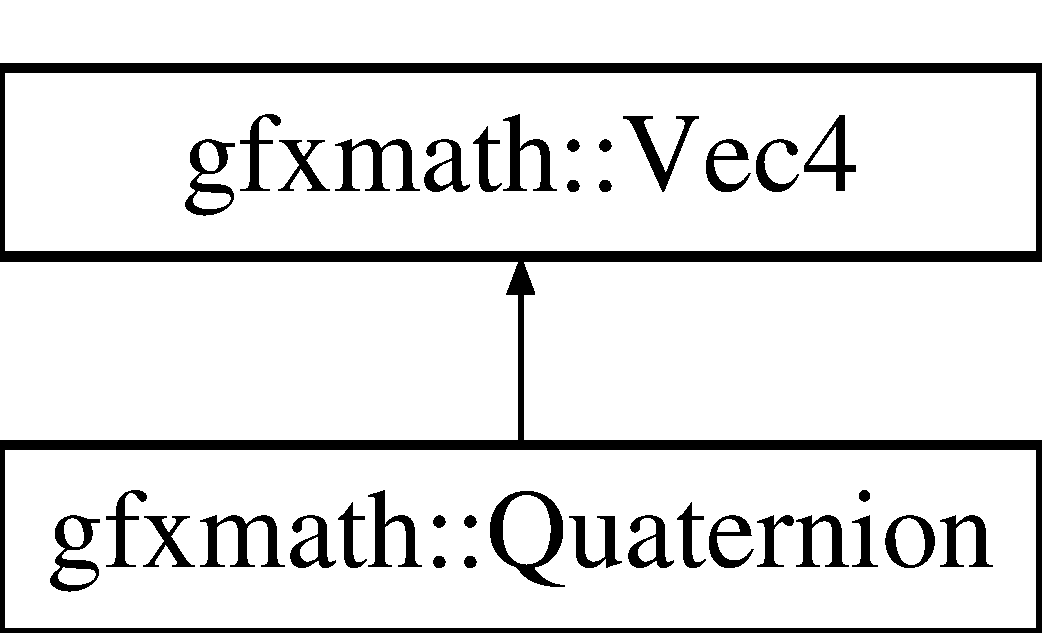
\includegraphics[height=2.000000cm]{classgfxmath_1_1_vec4}
\end{center}
\end{figure}
\subsection*{Public Member Functions}
\begin{DoxyCompactItemize}
\item 
\hyperlink{classgfxmath_1_1_vec4_a86e3b18e88af7f0d85629b01da04f2e9}{Vec4} ()
\begin{DoxyCompactList}\small\item\em Constructs a \hyperlink{classgfxmath_1_1_vec4}{Vec4} with all four components being initialized to 0.\+0f. \end{DoxyCompactList}\item 
\hyperlink{classgfxmath_1_1_vec4_a6ab39b817f6eeac365ee31ddf76635f9}{Vec4} (float xyzw)
\begin{DoxyCompactList}\small\item\em Constructor taking a single float argument that will be copied into all four component values. \end{DoxyCompactList}\item 
\hyperlink{classgfxmath_1_1_vec4_a77430bab02f56509bb3455863972ad8a}{Vec4} (float \hyperlink{classgfxmath_1_1_vec4_a273598aff75406f0e7a47121b8b06037}{x}, float \hyperlink{classgfxmath_1_1_vec4_a95e0ca27d66d7e0223606c20d326b595}{y}, float \hyperlink{classgfxmath_1_1_vec4_acd626b757468a5ea39f98812a36c4419}{z}, float \hyperlink{classgfxmath_1_1_vec4_adf2769a47b464dfee8d04e191f21701e}{w})
\begin{DoxyCompactList}\small\item\em Constructor taking four separate component values to use for the respective coordinate components of this \hyperlink{classgfxmath_1_1_vec4}{Vec4}. \end{DoxyCompactList}\item 
\hyperlink{classgfxmath_1_1_vec4_a426ca21da0ff954f7aded1982166f549}{Vec4} (const \hyperlink{classgfxmath_1_1_vec2}{Vec2} \&xy, const \hyperlink{classgfxmath_1_1_vec2}{Vec2} \&zw)
\begin{DoxyCompactList}\small\item\em Constructor that takes two \hyperlink{classgfxmath_1_1_vec2}{Vec2} arguments and copies their values into the first and second pair of components, respectively. \end{DoxyCompactList}\item 
\hyperlink{classgfxmath_1_1_vec4_af296766fa56d041e2478646f1ee9b081}{Vec4} (const \hyperlink{classgfxmath_1_1_vec2}{Vec2} \&xy, float \hyperlink{classgfxmath_1_1_vec4_acd626b757468a5ea39f98812a36c4419}{z}, float \hyperlink{classgfxmath_1_1_vec4_adf2769a47b464dfee8d04e191f21701e}{w})
\begin{DoxyCompactList}\small\item\em Constructor taking a \hyperlink{classgfxmath_1_1_vec2}{Vec2} for the x and y-\/component values, then two separate floats for the z and w-\/coordinate component values. \end{DoxyCompactList}\item 
\hyperlink{classgfxmath_1_1_vec4_a8211b449c2b1bbd084a7afb023525a03}{Vec4} (float \hyperlink{classgfxmath_1_1_vec4_a273598aff75406f0e7a47121b8b06037}{x}, const \hyperlink{classgfxmath_1_1_vec2}{Vec2} \&yz, float \hyperlink{classgfxmath_1_1_vec4_adf2769a47b464dfee8d04e191f21701e}{w})
\begin{DoxyCompactList}\small\item\em Constructor taking a single float for the x-\/coordinate component, followed by a \hyperlink{classgfxmath_1_1_vec2}{Vec2} for the y and z-\/coordinate component values, then another floats for the w-\/coordinate component. \end{DoxyCompactList}\item 
\hyperlink{classgfxmath_1_1_vec4_a1565b9d0e01810e9b9cbe4fc2c82055c}{Vec4} (float \hyperlink{classgfxmath_1_1_vec4_a273598aff75406f0e7a47121b8b06037}{x}, float \hyperlink{classgfxmath_1_1_vec4_a95e0ca27d66d7e0223606c20d326b595}{y}, const \hyperlink{classgfxmath_1_1_vec2}{Vec2} \&zw)
\begin{DoxyCompactList}\small\item\em Constructor taking two float values for the x and y-\/coordinate component values, followed by a \hyperlink{classgfxmath_1_1_vec2}{Vec2} for the z and w-\/coordinate component values. \end{DoxyCompactList}\item 
\hyperlink{classgfxmath_1_1_vec4_a115b5e4a0a51582b23f058ad225843b1}{Vec4} (const \hyperlink{classgfxmath_1_1_vec3}{Vec3} \&xyz, float \hyperlink{classgfxmath_1_1_vec4_adf2769a47b464dfee8d04e191f21701e}{w})
\begin{DoxyCompactList}\small\item\em Constructor taking a single \hyperlink{classgfxmath_1_1_vec3}{Vec3} for the x, y, and z-\/coordinate component values, followed by a single float for the w-\/coordinate component value. \end{DoxyCompactList}\item 
\hyperlink{classgfxmath_1_1_vec4_a43924f8c2f48fc84c10bba432921d6cc}{Vec4} (float \hyperlink{classgfxmath_1_1_vec4_a273598aff75406f0e7a47121b8b06037}{x}, const \hyperlink{classgfxmath_1_1_vec3}{Vec3} \&yzw)
\begin{DoxyCompactList}\small\item\em Constructor taking a single float for the w-\/coordinate component value, followed by a single \hyperlink{classgfxmath_1_1_vec3}{Vec3} for the x, y, and z-\/coordinate component values. \end{DoxyCompactList}\item 
\hyperlink{classgfxmath_1_1_vec4_ad62fa2df15d4caf6e62b1a1374dc6ea7}{operator Vec2} () const 
\begin{DoxyCompactList}\small\item\em Explicit cast that converts the given to a \hyperlink{classgfxmath_1_1_vec2}{Vec2}. \end{DoxyCompactList}\item 
\hyperlink{classgfxmath_1_1_vec4_a451f6c531cdd3615faaf9c2fc014e4c5}{operator Vec3} () const 
\begin{DoxyCompactList}\small\item\em Explicit cast that converts the given to a \hyperlink{classgfxmath_1_1_vec3}{Vec3}. \end{DoxyCompactList}\item 
\hyperlink{classgfxmath_1_1_vec4_aaf08e3ea9dc716a152e096276d89f429}{operator Quaternion} () const 
\begin{DoxyCompactList}\small\item\em Explicit cast that converts the given to a \hyperlink{classgfxmath_1_1_quaternion}{Quaternion}. \end{DoxyCompactList}\end{DoxyCompactItemize}
\subsection*{Static Public Member Functions}
\begin{DoxyCompactItemize}
\item 
\hypertarget{classgfxmath_1_1_vec4_ab33520d34d2602f623c11594f5ed2f7d}{}static \hyperlink{classgfxmath_1_1_vec4}{Vec4} \hyperlink{classgfxmath_1_1_vec4_ab33520d34d2602f623c11594f5ed2f7d}{E0} ()\label{classgfxmath_1_1_vec4_ab33520d34d2602f623c11594f5ed2f7d}

\begin{DoxyCompactList}\small\item\em The elementary vector with components $<$1 0 0 0$>$ \end{DoxyCompactList}\item 
\hypertarget{classgfxmath_1_1_vec4_a8b088082a24053becfc32a669bba4e93}{}static \hyperlink{classgfxmath_1_1_vec4}{Vec4} \hyperlink{classgfxmath_1_1_vec4_a8b088082a24053becfc32a669bba4e93}{E1} ()\label{classgfxmath_1_1_vec4_a8b088082a24053becfc32a669bba4e93}

\begin{DoxyCompactList}\small\item\em The elementary vector with components $<$0 1 0 0$>$ \end{DoxyCompactList}\item 
\hypertarget{classgfxmath_1_1_vec4_a729213a952a975ba9c41538d136ec3f2}{}static \hyperlink{classgfxmath_1_1_vec4}{Vec4} \hyperlink{classgfxmath_1_1_vec4_a729213a952a975ba9c41538d136ec3f2}{E2} ()\label{classgfxmath_1_1_vec4_a729213a952a975ba9c41538d136ec3f2}

\begin{DoxyCompactList}\small\item\em The elementary vector with components $<$0 0 1 0$>$ \end{DoxyCompactList}\item 
\hypertarget{classgfxmath_1_1_vec4_aed404d6e82c29c918b47bb9f39b29ae2}{}static \hyperlink{classgfxmath_1_1_vec4}{Vec4} \hyperlink{classgfxmath_1_1_vec4_aed404d6e82c29c918b47bb9f39b29ae2}{E3} ()\label{classgfxmath_1_1_vec4_aed404d6e82c29c918b47bb9f39b29ae2}

\begin{DoxyCompactList}\small\item\em The elementary vector with components $<$0 0 0 1$>$ \end{DoxyCompactList}\item 
\hypertarget{classgfxmath_1_1_vec4_ad821eb6978366575d602aaa0bbe54c3c}{}static \hyperlink{classgfxmath_1_1_vec4}{Vec4} \hyperlink{classgfxmath_1_1_vec4_ad821eb6978366575d602aaa0bbe54c3c}{E} (int i)\label{classgfxmath_1_1_vec4_ad821eb6978366575d602aaa0bbe54c3c}

\begin{DoxyCompactList}\small\item\em The array of elementary 4-\/component vectors. \end{DoxyCompactList}\item 
\hypertarget{classgfxmath_1_1_vec4_ae7e679c76f77752af8278adbc3000184}{}static \hyperlink{classgfxmath_1_1_vec4}{Vec4} \hyperlink{classgfxmath_1_1_vec4_ae7e679c76f77752af8278adbc3000184}{Neg\+E0} ()\label{classgfxmath_1_1_vec4_ae7e679c76f77752af8278adbc3000184}

\begin{DoxyCompactList}\small\item\em The negative form of the first elementary vector (takes the form $<$-\/1 0 0 0$>$) \end{DoxyCompactList}\item 
\hypertarget{classgfxmath_1_1_vec4_a2621b87b8c36463449af56ab020de208}{}static \hyperlink{classgfxmath_1_1_vec4}{Vec4} \hyperlink{classgfxmath_1_1_vec4_a2621b87b8c36463449af56ab020de208}{Neg\+E1} ()\label{classgfxmath_1_1_vec4_a2621b87b8c36463449af56ab020de208}

\begin{DoxyCompactList}\small\item\em The negative form of the second elementary vector (takes the form $<$0 -\/1 0 0$>$) \end{DoxyCompactList}\item 
\hypertarget{classgfxmath_1_1_vec4_ad27cfa3be5c0d7a531631cd7736d14c2}{}static \hyperlink{classgfxmath_1_1_vec4}{Vec4} \hyperlink{classgfxmath_1_1_vec4_ad27cfa3be5c0d7a531631cd7736d14c2}{Neg\+E2} ()\label{classgfxmath_1_1_vec4_ad27cfa3be5c0d7a531631cd7736d14c2}

\begin{DoxyCompactList}\small\item\em The negative form of the third elementary vector (takes the form $<$ 0 0 -\/1 0$>$) \end{DoxyCompactList}\item 
\hypertarget{classgfxmath_1_1_vec4_aba48145b1201b7e438bcdf84cd81620f}{}static \hyperlink{classgfxmath_1_1_vec4}{Vec4} \hyperlink{classgfxmath_1_1_vec4_aba48145b1201b7e438bcdf84cd81620f}{Neg\+E3} ()\label{classgfxmath_1_1_vec4_aba48145b1201b7e438bcdf84cd81620f}

\begin{DoxyCompactList}\small\item\em The negative form of the fourth elementary vector (takes the form $<$0 0 0 -\/1$>$) \end{DoxyCompactList}\item 
\hypertarget{classgfxmath_1_1_vec4_a8b1d7c4394f167b788391351c981d79b}{}static \hyperlink{classgfxmath_1_1_vec4}{Vec4} \hyperlink{classgfxmath_1_1_vec4_a8b1d7c4394f167b788391351c981d79b}{Neg\+E} (int i)\label{classgfxmath_1_1_vec4_a8b1d7c4394f167b788391351c981d79b}

\begin{DoxyCompactList}\small\item\em The array of negated elementary 4-\/component vectors. \end{DoxyCompactList}\item 
\hypertarget{classgfxmath_1_1_vec4_a533973443903b6fdc0e194e1f6c9b5ae}{}static \hyperlink{classgfxmath_1_1_vec4}{Vec4} \hyperlink{classgfxmath_1_1_vec4_a533973443903b6fdc0e194e1f6c9b5ae}{One} ()\label{classgfxmath_1_1_vec4_a533973443903b6fdc0e194e1f6c9b5ae}

\begin{DoxyCompactList}\small\item\em The 4-\/component vector containing the values $<$1 1 1 1$>$ \end{DoxyCompactList}\item 
\hypertarget{classgfxmath_1_1_vec4_a5c21fa07daf7054e189820c05bc2e0ee}{}static \hyperlink{classgfxmath_1_1_vec4}{Vec4} \hyperlink{classgfxmath_1_1_vec4_a5c21fa07daf7054e189820c05bc2e0ee}{Neg\+One} ()\label{classgfxmath_1_1_vec4_a5c21fa07daf7054e189820c05bc2e0ee}

\begin{DoxyCompactList}\small\item\em The 4-\/component vector containing the values $<$-\/1 -\/1 -\/1 -\/1$>$ \end{DoxyCompactList}\item 
\hypertarget{classgfxmath_1_1_vec4_aaacd0ad4911f4a53f82cc6979082b5c8}{}static \hyperlink{classgfxmath_1_1_vec4}{Vec4} \hyperlink{classgfxmath_1_1_vec4_aaacd0ad4911f4a53f82cc6979082b5c8}{Zero} ()\label{classgfxmath_1_1_vec4_aaacd0ad4911f4a53f82cc6979082b5c8}

\begin{DoxyCompactList}\small\item\em The 4-\/component zero vector (takes the form $<$0 0 0 0$>$ \end{DoxyCompactList}\end{DoxyCompactItemize}
\subsection*{Public Attributes}
\begin{DoxyCompactItemize}
\item 
float \hyperlink{classgfxmath_1_1_vec4_aa668d284af0138ed1d09663fb0bd3d6f}{vals} \mbox{[}4\mbox{]}
\begin{DoxyCompactList}\small\item\em The 4 components of the \hyperlink{classgfxmath_1_1_vec4}{Vec4}. \end{DoxyCompactList}\item 
float \hyperlink{classgfxmath_1_1_vec4_a273598aff75406f0e7a47121b8b06037}{x}
\begin{DoxyCompactList}\small\item\em The x-\/coordinate. \end{DoxyCompactList}\item 
float \hyperlink{classgfxmath_1_1_vec4_a95e0ca27d66d7e0223606c20d326b595}{y}
\begin{DoxyCompactList}\small\item\em The y-\/coordinate. \end{DoxyCompactList}\item 
float \hyperlink{classgfxmath_1_1_vec4_acd626b757468a5ea39f98812a36c4419}{z}
\begin{DoxyCompactList}\small\item\em The z-\/coordinate. \end{DoxyCompactList}\item 
float \hyperlink{classgfxmath_1_1_vec4_adf2769a47b464dfee8d04e191f21701e}{w}
\begin{DoxyCompactList}\small\item\em The w-\/coordinate. \end{DoxyCompactList}\end{DoxyCompactItemize}
\subsection*{Friends}
\begin{DoxyCompactItemize}
\item 
std\+::ostream \& \hyperlink{classgfxmath_1_1_vec4_a31c794bedecdf686aae40b9261ea38c5}{operator$<$$<$} (std\+::ostream \&stream, const \hyperlink{classgfxmath_1_1_vec4}{Vec4} \&vec)
\begin{DoxyCompactList}\small\item\em A function that writes the given 4\+D vector to the given output stream. \end{DoxyCompactList}\item 
std\+::istream \& \hyperlink{classgfxmath_1_1_vec4_ab5d34a5bf6bb543ab690436fc45c7319}{operator$>$$>$} (std\+::istream \&stream, \hyperlink{classgfxmath_1_1_vec4}{Vec4} \&vec)
\begin{DoxyCompactList}\small\item\em A function that reads in the a 4\+D vector from the given input stream. \end{DoxyCompactList}\item 
bool \hyperlink{classgfxmath_1_1_vec4_a75ec0a4eb1bdb2abb83280b62f2e94d3}{operator==} (const \hyperlink{classgfxmath_1_1_vec4}{Vec4} \&left, const \hyperlink{classgfxmath_1_1_vec4}{Vec4} \&right)
\begin{DoxyCompactList}\small\item\em Equality operator. \end{DoxyCompactList}\item 
bool \hyperlink{classgfxmath_1_1_vec4_a8ddc017b9087be64efa4fc76f1f63a12}{operator!=} (const \hyperlink{classgfxmath_1_1_vec4}{Vec4} \&left, const \hyperlink{classgfxmath_1_1_vec4}{Vec4} \&right)
\begin{DoxyCompactList}\small\item\em Inequality operator. \end{DoxyCompactList}\end{DoxyCompactItemize}
\subsection*{Related Functions}
(Note that these are not member functions.) {\bf }\par
\begin{DoxyCompactItemize}
\item 
\hyperlink{classgfxmath_1_1_vec4}{Vec4} \hyperlink{classgfxmath_1_1_vec4_a8812efd4565ada77e6dab63828ad715b}{Vec4\+Add} (const \hyperlink{classgfxmath_1_1_vec4}{Vec4} \&first, const \hyperlink{classgfxmath_1_1_vec4}{Vec4} \&second)
\begin{DoxyCompactList}\small\item\em Add the two given Vec4s. \end{DoxyCompactList}\item 
\hyperlink{classgfxmath_1_1_vec4}{Vec4} \hyperlink{classgfxmath_1_1_vec4_a01968b83532d01613a8f89659d4a52dc}{Vec4\+Sub} (const \hyperlink{classgfxmath_1_1_vec4}{Vec4} \&first, const \hyperlink{classgfxmath_1_1_vec4}{Vec4} \&second)
\begin{DoxyCompactList}\small\item\em Subtract the two given Vec4s. \end{DoxyCompactList}\item 
float \hyperlink{classgfxmath_1_1_vec4_a2deb01c8dd6f1a06c0a0cfc2e96e9c1e}{Vec4\+Dot} (const \hyperlink{classgfxmath_1_1_vec4}{Vec4} \&first, const \hyperlink{classgfxmath_1_1_vec4}{Vec4} \&second)
\begin{DoxyCompactList}\small\item\em \hyperlink{classgfxmath_1_1_vec4}{Vec4} dot product. \end{DoxyCompactList}\item 
\hyperlink{classgfxmath_1_1_vec4}{Vec4} \hyperlink{classgfxmath_1_1_vec4_a70441f2888f0df752fe0624a5a7b362d}{Vec4\+Mul\+Scalar} (const \hyperlink{classgfxmath_1_1_vec4}{Vec4} \&vec, float factor)
\begin{DoxyCompactList}\small\item\em Multiply the components of the given \hyperlink{classgfxmath_1_1_vec4}{Vec4} by the given scalar. \end{DoxyCompactList}\item 
\hyperlink{classgfxmath_1_1_vec4}{Vec4} \hyperlink{classgfxmath_1_1_vec4_a670f1f6ebdadeaa2f656f153218fdee8}{Vec4\+Div\+Scalar} (const \hyperlink{classgfxmath_1_1_vec4}{Vec4} \&vec, float divisor)
\begin{DoxyCompactList}\small\item\em Divide the components of the given \hyperlink{classgfxmath_1_1_vec4}{Vec4} by the given scalar. \end{DoxyCompactList}\item 
\hyperlink{classgfxmath_1_1_vec4}{Vec4} \hyperlink{classgfxmath_1_1_vec4_af1fa3fbf9843a509f3b8a476aa18361b}{Vec4\+Normalize} (const \hyperlink{classgfxmath_1_1_vec4}{Vec4} \&vec)
\begin{DoxyCompactList}\small\item\em Normalize the given \hyperlink{classgfxmath_1_1_vec4}{Vec4}. \end{DoxyCompactList}\item 
\hyperlink{classgfxmath_1_1_vec4}{Vec4} \hyperlink{classgfxmath_1_1_vec4_a9ba6951d54c6a4d9d513580f5bf3b928}{Vec4\+Negate} (const \hyperlink{classgfxmath_1_1_vec4}{Vec4} \&vec)
\begin{DoxyCompactList}\small\item\em Negate the given \hyperlink{classgfxmath_1_1_vec4}{Vec4} components. \end{DoxyCompactList}\item 
{\footnotesize template$<$Float\+Precision precision = Float\+Precision\+::\+H\+I\+G\+H$>$ }\\bool \hyperlink{classgfxmath_1_1_vec4_a819b8c958e12f0838288c641af7e1ab6}{Vec4\+Approx\+Equal} (const \hyperlink{classgfxmath_1_1_vec4}{Vec4} \&first, const \hyperlink{classgfxmath_1_1_vec4}{Vec4} \&second)
\begin{DoxyCompactList}\small\item\em Determines whether the two Vec4s are approximately equal, based on the given Precision template argument (defaults to H\+I\+G\+H precision). \end{DoxyCompactList}\item 
bool \hyperlink{classgfxmath_1_1_vec4_ab82fdfebe73934664b56e9ba1174f37f}{Vec4\+Has\+Na\+N} (const \hyperlink{classgfxmath_1_1_vec4}{Vec4} \&vec)
\begin{DoxyCompactList}\small\item\em Vector 2 has a Na\+N component value. \end{DoxyCompactList}\item 
bool \hyperlink{classgfxmath_1_1_vec4_a29cd467d514b701c3a796cb75234be0b}{Vec4\+Has\+Infinite} (const \hyperlink{classgfxmath_1_1_vec4}{Vec4} \&vec)
\begin{DoxyCompactList}\small\item\em Determines whether or not the given \hyperlink{classgfxmath_1_1_vec4}{Vec4} has an infinite value component. \end{DoxyCompactList}\end{DoxyCompactItemize}



\subsection{Detailed Description}
A mathematical vector with 4 components. 

\subsection{Constructor \& Destructor Documentation}
\hypertarget{classgfxmath_1_1_vec4_a86e3b18e88af7f0d85629b01da04f2e9}{}\index{gfxmath\+::\+Vec4@{gfxmath\+::\+Vec4}!Vec4@{Vec4}}
\index{Vec4@{Vec4}!gfxmath\+::\+Vec4@{gfxmath\+::\+Vec4}}
\subsubsection[{Vec4}]{\setlength{\rightskip}{0pt plus 5cm}gfxmath\+::\+Vec4\+::\+Vec4 (
\begin{DoxyParamCaption}
{}
\end{DoxyParamCaption}
)}\label{classgfxmath_1_1_vec4_a86e3b18e88af7f0d85629b01da04f2e9}


Constructs a \hyperlink{classgfxmath_1_1_vec4}{Vec4} with all four components being initialized to 0.\+0f. 

\begin{DoxyDate}{Date}
2/22/2015 
\end{DoxyDate}
\hypertarget{classgfxmath_1_1_vec4_a6ab39b817f6eeac365ee31ddf76635f9}{}\index{gfxmath\+::\+Vec4@{gfxmath\+::\+Vec4}!Vec4@{Vec4}}
\index{Vec4@{Vec4}!gfxmath\+::\+Vec4@{gfxmath\+::\+Vec4}}
\subsubsection[{Vec4}]{\setlength{\rightskip}{0pt plus 5cm}gfxmath\+::\+Vec4\+::\+Vec4 (
\begin{DoxyParamCaption}
\item[{float}]{xyzw}
\end{DoxyParamCaption}
)}\label{classgfxmath_1_1_vec4_a6ab39b817f6eeac365ee31ddf76635f9}


Constructor taking a single float argument that will be copied into all four component values. 

\begin{DoxyDate}{Date}
2/22/2015
\end{DoxyDate}

\begin{DoxyParams}{Parameters}
{\em xyzw} & The value that will be copied into the x, y, z, and w components. \\
\hline
\end{DoxyParams}
\hypertarget{classgfxmath_1_1_vec4_a77430bab02f56509bb3455863972ad8a}{}\index{gfxmath\+::\+Vec4@{gfxmath\+::\+Vec4}!Vec4@{Vec4}}
\index{Vec4@{Vec4}!gfxmath\+::\+Vec4@{gfxmath\+::\+Vec4}}
\subsubsection[{Vec4}]{\setlength{\rightskip}{0pt plus 5cm}gfxmath\+::\+Vec4\+::\+Vec4 (
\begin{DoxyParamCaption}
\item[{float}]{x, }
\item[{float}]{y, }
\item[{float}]{z, }
\item[{float}]{w}
\end{DoxyParamCaption}
)}\label{classgfxmath_1_1_vec4_a77430bab02f56509bb3455863972ad8a}


Constructor taking four separate component values to use for the respective coordinate components of this \hyperlink{classgfxmath_1_1_vec4}{Vec4}. 

\begin{DoxyDate}{Date}
2/22/2015
\end{DoxyDate}

\begin{DoxyParams}{Parameters}
{\em x} & The x-\/coordinate component value of this \hyperlink{classgfxmath_1_1_vec4}{Vec4}. \\
\hline
{\em y} & The y-\/coordinate component value of this \hyperlink{classgfxmath_1_1_vec4}{Vec4}. \\
\hline
{\em z} & The z-\/coordinate component value of this \hyperlink{classgfxmath_1_1_vec4}{Vec4}. \\
\hline
{\em w} & The w-\/coordinate component value of this \hyperlink{classgfxmath_1_1_vec4}{Vec4}. \\
\hline
\end{DoxyParams}
\hypertarget{classgfxmath_1_1_vec4_a426ca21da0ff954f7aded1982166f549}{}\index{gfxmath\+::\+Vec4@{gfxmath\+::\+Vec4}!Vec4@{Vec4}}
\index{Vec4@{Vec4}!gfxmath\+::\+Vec4@{gfxmath\+::\+Vec4}}
\subsubsection[{Vec4}]{\setlength{\rightskip}{0pt plus 5cm}gfxmath\+::\+Vec4\+::\+Vec4 (
\begin{DoxyParamCaption}
\item[{const {\bf Vec2} \&}]{xy, }
\item[{const {\bf Vec2} \&}]{zw}
\end{DoxyParamCaption}
)}\label{classgfxmath_1_1_vec4_a426ca21da0ff954f7aded1982166f549}


Constructor that takes two \hyperlink{classgfxmath_1_1_vec2}{Vec2} arguments and copies their values into the first and second pair of components, respectively. 

\begin{DoxyDate}{Date}
2/22/2015
\end{DoxyDate}

\begin{DoxyParams}{Parameters}
{\em xy} & The \hyperlink{classgfxmath_1_1_vec2}{Vec2} that will contribute its components to the x and y-\/coordinate components of this \hyperlink{classgfxmath_1_1_vec4}{Vec4}. \\
\hline
{\em zw} & The \hyperlink{classgfxmath_1_1_vec2}{Vec2} that will contribute its components to the z and w-\/coordinate components of this \hyperlink{classgfxmath_1_1_vec4}{Vec4}. \\
\hline
\end{DoxyParams}
\hypertarget{classgfxmath_1_1_vec4_af296766fa56d041e2478646f1ee9b081}{}\index{gfxmath\+::\+Vec4@{gfxmath\+::\+Vec4}!Vec4@{Vec4}}
\index{Vec4@{Vec4}!gfxmath\+::\+Vec4@{gfxmath\+::\+Vec4}}
\subsubsection[{Vec4}]{\setlength{\rightskip}{0pt plus 5cm}gfxmath\+::\+Vec4\+::\+Vec4 (
\begin{DoxyParamCaption}
\item[{const {\bf Vec2} \&}]{xy, }
\item[{float}]{z, }
\item[{float}]{w}
\end{DoxyParamCaption}
)}\label{classgfxmath_1_1_vec4_af296766fa56d041e2478646f1ee9b081}


Constructor taking a \hyperlink{classgfxmath_1_1_vec2}{Vec2} for the x and y-\/component values, then two separate floats for the z and w-\/coordinate component values. 

\begin{DoxyDate}{Date}
2/22/2015
\end{DoxyDate}

\begin{DoxyParams}{Parameters}
{\em xy} & The \hyperlink{classgfxmath_1_1_vec2}{Vec2} that will contribute its components to the x and y-\/coordinate components of this \hyperlink{classgfxmath_1_1_vec4}{Vec4}. \\
\hline
{\em z} & The z-\/coordinate component value of this \hyperlink{classgfxmath_1_1_vec4}{Vec4}. \\
\hline
{\em w} & The w-\/coordinate component value of this \hyperlink{classgfxmath_1_1_vec4}{Vec4}. \\
\hline
\end{DoxyParams}
\hypertarget{classgfxmath_1_1_vec4_a8211b449c2b1bbd084a7afb023525a03}{}\index{gfxmath\+::\+Vec4@{gfxmath\+::\+Vec4}!Vec4@{Vec4}}
\index{Vec4@{Vec4}!gfxmath\+::\+Vec4@{gfxmath\+::\+Vec4}}
\subsubsection[{Vec4}]{\setlength{\rightskip}{0pt plus 5cm}gfxmath\+::\+Vec4\+::\+Vec4 (
\begin{DoxyParamCaption}
\item[{float}]{x, }
\item[{const {\bf Vec2} \&}]{yz, }
\item[{float}]{w}
\end{DoxyParamCaption}
)}\label{classgfxmath_1_1_vec4_a8211b449c2b1bbd084a7afb023525a03}


Constructor taking a single float for the x-\/coordinate component, followed by a \hyperlink{classgfxmath_1_1_vec2}{Vec2} for the y and z-\/coordinate component values, then another floats for the w-\/coordinate component. 

\begin{DoxyDate}{Date}
2/22/2015
\end{DoxyDate}

\begin{DoxyParams}{Parameters}
{\em x} & The x-\/coordinate component value of this \hyperlink{classgfxmath_1_1_vec4}{Vec4}. \\
\hline
{\em yz} & The \hyperlink{classgfxmath_1_1_vec2}{Vec2} that will contribute its components to the y and z-\/coordinate components of this \hyperlink{classgfxmath_1_1_vec4}{Vec4}. \\
\hline
{\em w} & The w-\/coordinate component value of this \hyperlink{classgfxmath_1_1_vec4}{Vec4}. \\
\hline
\end{DoxyParams}
\hypertarget{classgfxmath_1_1_vec4_a1565b9d0e01810e9b9cbe4fc2c82055c}{}\index{gfxmath\+::\+Vec4@{gfxmath\+::\+Vec4}!Vec4@{Vec4}}
\index{Vec4@{Vec4}!gfxmath\+::\+Vec4@{gfxmath\+::\+Vec4}}
\subsubsection[{Vec4}]{\setlength{\rightskip}{0pt plus 5cm}gfxmath\+::\+Vec4\+::\+Vec4 (
\begin{DoxyParamCaption}
\item[{float}]{x, }
\item[{float}]{y, }
\item[{const {\bf Vec2} \&}]{zw}
\end{DoxyParamCaption}
)}\label{classgfxmath_1_1_vec4_a1565b9d0e01810e9b9cbe4fc2c82055c}


Constructor taking two float values for the x and y-\/coordinate component values, followed by a \hyperlink{classgfxmath_1_1_vec2}{Vec2} for the z and w-\/coordinate component values. 

\begin{DoxyDate}{Date}
2/22/2015
\end{DoxyDate}

\begin{DoxyParams}{Parameters}
{\em x} & The x-\/coordinate component value of this \hyperlink{classgfxmath_1_1_vec4}{Vec4}. \\
\hline
{\em y} & The y-\/coordinate component value of this \hyperlink{classgfxmath_1_1_vec4}{Vec4}. \\
\hline
{\em zw} & The \hyperlink{classgfxmath_1_1_vec2}{Vec2} that will contribute its components to the z and w-\/coordinate components of this \hyperlink{classgfxmath_1_1_vec4}{Vec4}. \\
\hline
\end{DoxyParams}
\hypertarget{classgfxmath_1_1_vec4_a115b5e4a0a51582b23f058ad225843b1}{}\index{gfxmath\+::\+Vec4@{gfxmath\+::\+Vec4}!Vec4@{Vec4}}
\index{Vec4@{Vec4}!gfxmath\+::\+Vec4@{gfxmath\+::\+Vec4}}
\subsubsection[{Vec4}]{\setlength{\rightskip}{0pt plus 5cm}gfxmath\+::\+Vec4\+::\+Vec4 (
\begin{DoxyParamCaption}
\item[{const {\bf Vec3} \&}]{xyz, }
\item[{float}]{w}
\end{DoxyParamCaption}
)}\label{classgfxmath_1_1_vec4_a115b5e4a0a51582b23f058ad225843b1}


Constructor taking a single \hyperlink{classgfxmath_1_1_vec3}{Vec3} for the x, y, and z-\/coordinate component values, followed by a single float for the w-\/coordinate component value. 

\begin{DoxyDate}{Date}
2/22/2015
\end{DoxyDate}

\begin{DoxyParams}{Parameters}
{\em xyz} & The \hyperlink{classgfxmath_1_1_vec3}{Vec3} that will contribute its components to the x, y and z-\/coordinate components of this \hyperlink{classgfxmath_1_1_vec4}{Vec4}. \\
\hline
{\em w} & The w-\/coordinate component value of this \hyperlink{classgfxmath_1_1_vec4}{Vec4}. \\
\hline
\end{DoxyParams}
\hypertarget{classgfxmath_1_1_vec4_a43924f8c2f48fc84c10bba432921d6cc}{}\index{gfxmath\+::\+Vec4@{gfxmath\+::\+Vec4}!Vec4@{Vec4}}
\index{Vec4@{Vec4}!gfxmath\+::\+Vec4@{gfxmath\+::\+Vec4}}
\subsubsection[{Vec4}]{\setlength{\rightskip}{0pt plus 5cm}gfxmath\+::\+Vec4\+::\+Vec4 (
\begin{DoxyParamCaption}
\item[{float}]{x, }
\item[{const {\bf Vec3} \&}]{yzw}
\end{DoxyParamCaption}
)}\label{classgfxmath_1_1_vec4_a43924f8c2f48fc84c10bba432921d6cc}


Constructor taking a single float for the w-\/coordinate component value, followed by a single \hyperlink{classgfxmath_1_1_vec3}{Vec3} for the x, y, and z-\/coordinate component values. 

\begin{DoxyDate}{Date}
2/22/2015
\end{DoxyDate}

\begin{DoxyParams}{Parameters}
{\em x} & The x-\/coordinate component value of this \hyperlink{classgfxmath_1_1_vec4}{Vec4}. \\
\hline
{\em yzw} & The \hyperlink{classgfxmath_1_1_vec3}{Vec3} that will contribute its components to the y, z and w-\/coordinate components of this \hyperlink{classgfxmath_1_1_vec4}{Vec4}. \\
\hline
\end{DoxyParams}


\subsection{Member Function Documentation}
\hypertarget{classgfxmath_1_1_vec4_aaf08e3ea9dc716a152e096276d89f429}{}\index{gfxmath\+::\+Vec4@{gfxmath\+::\+Vec4}!operator Quaternion@{operator Quaternion}}
\index{operator Quaternion@{operator Quaternion}!gfxmath\+::\+Vec4@{gfxmath\+::\+Vec4}}
\subsubsection[{operator Quaternion}]{\setlength{\rightskip}{0pt plus 5cm}gfxmath\+::\+Vec4\+::operator {\bf Quaternion} (
\begin{DoxyParamCaption}
{}
\end{DoxyParamCaption}
) const\hspace{0.3cm}{\ttfamily [explicit]}}\label{classgfxmath_1_1_vec4_aaf08e3ea9dc716a152e096276d89f429}


Explicit cast that converts the given to a \hyperlink{classgfxmath_1_1_quaternion}{Quaternion}. 

\begin{DoxyDate}{Date}
2/22/2015
\end{DoxyDate}
\begin{DoxyReturn}{Returns}
The result of the operation. 
\end{DoxyReturn}
\hypertarget{classgfxmath_1_1_vec4_ad62fa2df15d4caf6e62b1a1374dc6ea7}{}\index{gfxmath\+::\+Vec4@{gfxmath\+::\+Vec4}!operator Vec2@{operator Vec2}}
\index{operator Vec2@{operator Vec2}!gfxmath\+::\+Vec4@{gfxmath\+::\+Vec4}}
\subsubsection[{operator Vec2}]{\setlength{\rightskip}{0pt plus 5cm}gfxmath\+::\+Vec4\+::operator {\bf Vec2} (
\begin{DoxyParamCaption}
{}
\end{DoxyParamCaption}
) const\hspace{0.3cm}{\ttfamily [explicit]}}\label{classgfxmath_1_1_vec4_ad62fa2df15d4caf6e62b1a1374dc6ea7}


Explicit cast that converts the given to a \hyperlink{classgfxmath_1_1_vec2}{Vec2}. 

\begin{DoxyDate}{Date}
2/22/2015
\end{DoxyDate}
\begin{DoxyReturn}{Returns}
The result of the operation. 
\end{DoxyReturn}
\hypertarget{classgfxmath_1_1_vec4_a451f6c531cdd3615faaf9c2fc014e4c5}{}\index{gfxmath\+::\+Vec4@{gfxmath\+::\+Vec4}!operator Vec3@{operator Vec3}}
\index{operator Vec3@{operator Vec3}!gfxmath\+::\+Vec4@{gfxmath\+::\+Vec4}}
\subsubsection[{operator Vec3}]{\setlength{\rightskip}{0pt plus 5cm}gfxmath\+::\+Vec4\+::operator {\bf Vec3} (
\begin{DoxyParamCaption}
{}
\end{DoxyParamCaption}
) const\hspace{0.3cm}{\ttfamily [explicit]}}\label{classgfxmath_1_1_vec4_a451f6c531cdd3615faaf9c2fc014e4c5}


Explicit cast that converts the given to a \hyperlink{classgfxmath_1_1_vec3}{Vec3}. 

\begin{DoxyDate}{Date}
2/22/2015
\end{DoxyDate}
\begin{DoxyReturn}{Returns}
The result of the operation. 
\end{DoxyReturn}


\subsection{Friends And Related Function Documentation}
\hypertarget{classgfxmath_1_1_vec4_a8ddc017b9087be64efa4fc76f1f63a12}{}\index{gfxmath\+::\+Vec4@{gfxmath\+::\+Vec4}!operator"!=@{operator"!=}}
\index{operator"!=@{operator"!=}!gfxmath\+::\+Vec4@{gfxmath\+::\+Vec4}}
\subsubsection[{operator"!=}]{\setlength{\rightskip}{0pt plus 5cm}bool operator!= (
\begin{DoxyParamCaption}
\item[{const {\bf Vec4} \&}]{left, }
\item[{const {\bf Vec4} \&}]{right}
\end{DoxyParamCaption}
)\hspace{0.3cm}{\ttfamily [friend]}}\label{classgfxmath_1_1_vec4_a8ddc017b9087be64efa4fc76f1f63a12}


Inequality operator. 

\begin{DoxyDate}{Date}
2/22/2015
\end{DoxyDate}

\begin{DoxyParams}{Parameters}
{\em left} & The first instance to compare. \\
\hline
{\em right} & The second instance to compare.\\
\hline
\end{DoxyParams}
\begin{DoxyReturn}{Returns}
true if the parameters are not considered equivalent. 
\end{DoxyReturn}
\hypertarget{classgfxmath_1_1_vec4_a31c794bedecdf686aae40b9261ea38c5}{}\index{gfxmath\+::\+Vec4@{gfxmath\+::\+Vec4}!operator$<$$<$@{operator$<$$<$}}
\index{operator$<$$<$@{operator$<$$<$}!gfxmath\+::\+Vec4@{gfxmath\+::\+Vec4}}
\subsubsection[{operator$<$$<$}]{\setlength{\rightskip}{0pt plus 5cm}std\+::ostream \& operator$<$$<$ (
\begin{DoxyParamCaption}
\item[{std\+::ostream \&}]{stream, }
\item[{const {\bf Vec4} \&}]{vec}
\end{DoxyParamCaption}
)\hspace{0.3cm}{\ttfamily [friend]}}\label{classgfxmath_1_1_vec4_a31c794bedecdf686aae40b9261ea38c5}


A function that writes the given 4\+D vector to the given output stream. 

\begin{DoxyDate}{Date}
2/22/2015
\end{DoxyDate}

\begin{DoxyParams}[1]{Parameters}
\mbox{\tt in,out}  & {\em stream} & The output stream to be written to. \\
\hline
 & {\em vec} & The \hyperlink{classgfxmath_1_1_vec4}{Vec4} to write to the stream.\\
\hline
\end{DoxyParams}
\begin{DoxyReturn}{Returns}
Writes the value of the given \hyperlink{classgfxmath_1_1_vec4}{Vec4} to the given output stream. 
\end{DoxyReturn}
\hypertarget{classgfxmath_1_1_vec4_a75ec0a4eb1bdb2abb83280b62f2e94d3}{}\index{gfxmath\+::\+Vec4@{gfxmath\+::\+Vec4}!operator==@{operator==}}
\index{operator==@{operator==}!gfxmath\+::\+Vec4@{gfxmath\+::\+Vec4}}
\subsubsection[{operator==}]{\setlength{\rightskip}{0pt plus 5cm}bool operator== (
\begin{DoxyParamCaption}
\item[{const {\bf Vec4} \&}]{left, }
\item[{const {\bf Vec4} \&}]{right}
\end{DoxyParamCaption}
)\hspace{0.3cm}{\ttfamily [friend]}}\label{classgfxmath_1_1_vec4_a75ec0a4eb1bdb2abb83280b62f2e94d3}


Equality operator. 

\begin{DoxyDate}{Date}
2/22/2015
\end{DoxyDate}

\begin{DoxyParams}{Parameters}
{\em left} & The first instance to compare. \\
\hline
{\em right} & The second instance to compare.\\
\hline
\end{DoxyParams}
\begin{DoxyReturn}{Returns}
true if the parameters are considered equivalent. 
\end{DoxyReturn}
\hypertarget{classgfxmath_1_1_vec4_ab5d34a5bf6bb543ab690436fc45c7319}{}\index{gfxmath\+::\+Vec4@{gfxmath\+::\+Vec4}!operator$>$$>$@{operator$>$$>$}}
\index{operator$>$$>$@{operator$>$$>$}!gfxmath\+::\+Vec4@{gfxmath\+::\+Vec4}}
\subsubsection[{operator$>$$>$}]{\setlength{\rightskip}{0pt plus 5cm}std\+::istream \& operator$>$$>$ (
\begin{DoxyParamCaption}
\item[{std\+::istream \&}]{stream, }
\item[{{\bf Vec4} \&}]{vec}
\end{DoxyParamCaption}
)\hspace{0.3cm}{\ttfamily [friend]}}\label{classgfxmath_1_1_vec4_ab5d34a5bf6bb543ab690436fc45c7319}


A function that reads in the a 4\+D vector from the given input stream. 

\begin{DoxyDate}{Date}
2/22/2015
\end{DoxyDate}

\begin{DoxyParams}[1]{Parameters}
\mbox{\tt in,out}  & {\em stream} & The input stream to be read from. \\
\hline
\mbox{\tt in,out}  & {\em vec} & The \hyperlink{classgfxmath_1_1_vec4}{Vec4} to read values into from the stream.\\
\hline
\end{DoxyParams}
\begin{DoxyReturn}{Returns}
Reads the value of the given input stream to the given \hyperlink{classgfxmath_1_1_vec4}{Vec4}. 
\end{DoxyReturn}
\hypertarget{classgfxmath_1_1_vec4_a8812efd4565ada77e6dab63828ad715b}{}\index{gfxmath\+::\+Vec4@{gfxmath\+::\+Vec4}!Vec4\+Add@{Vec4\+Add}}
\index{Vec4\+Add@{Vec4\+Add}!gfxmath\+::\+Vec4@{gfxmath\+::\+Vec4}}
\subsubsection[{Vec4\+Add}]{\setlength{\rightskip}{0pt plus 5cm}{\bf Vec4} Vec4\+Add (
\begin{DoxyParamCaption}
\item[{const {\bf Vec4} \&}]{first, }
\item[{const {\bf Vec4} \&}]{second}
\end{DoxyParamCaption}
)\hspace{0.3cm}{\ttfamily [related]}}\label{classgfxmath_1_1_vec4_a8812efd4565ada77e6dab63828ad715b}


Add the two given Vec4s. 

\begin{DoxyDate}{Date}
2/22/2015
\end{DoxyDate}

\begin{DoxyParams}{Parameters}
{\em first} & The first \hyperlink{classgfxmath_1_1_vec4}{Vec4} in the sum. \\
\hline
{\em second} & The second \hyperlink{classgfxmath_1_1_vec4}{Vec4} in the sum.\\
\hline
\end{DoxyParams}
\begin{DoxyReturn}{Returns}
The \hyperlink{classgfxmath_1_1_vec4}{Vec4} representing the sum of the two given Vec4s\textquotesingle{} components. 
\end{DoxyReturn}
\hypertarget{classgfxmath_1_1_vec4_a819b8c958e12f0838288c641af7e1ab6}{}\index{gfxmath\+::\+Vec4@{gfxmath\+::\+Vec4}!Vec4\+Approx\+Equal@{Vec4\+Approx\+Equal}}
\index{Vec4\+Approx\+Equal@{Vec4\+Approx\+Equal}!gfxmath\+::\+Vec4@{gfxmath\+::\+Vec4}}
\subsubsection[{Vec4\+Approx\+Equal}]{\setlength{\rightskip}{0pt plus 5cm}template$<$Float\+Precision precision = Float\+Precision\+::\+H\+I\+G\+H$>$ bool Vec4\+Approx\+Equal (
\begin{DoxyParamCaption}
\item[{const {\bf Vec4} \&}]{first, }
\item[{const {\bf Vec4} \&}]{second}
\end{DoxyParamCaption}
)\hspace{0.3cm}{\ttfamily [related]}}\label{classgfxmath_1_1_vec4_a819b8c958e12f0838288c641af7e1ab6}


Determines whether the two Vec4s are approximately equal, based on the given Precision template argument (defaults to H\+I\+G\+H precision). 

\begin{DoxyDate}{Date}
2/22/2015
\end{DoxyDate}

\begin{DoxyTemplParams}{Template Parameters}
{\em precision} & Type of the precision. \\
\hline
\end{DoxyTemplParams}

\begin{DoxyParams}{Parameters}
{\em first} & The first \hyperlink{classgfxmath_1_1_vec4}{Vec4} in the comparison. \\
\hline
{\em second} & The second \hyperlink{classgfxmath_1_1_vec4}{Vec4} in the comparison.\\
\hline
\end{DoxyParams}
\begin{DoxyReturn}{Returns}
true if the x, y, z and w components of the two given Vec4s have values that are within the Float\+Precision accuracy definition of one another, otherwise false. 
\end{DoxyReturn}
\hypertarget{classgfxmath_1_1_vec4_a670f1f6ebdadeaa2f656f153218fdee8}{}\index{gfxmath\+::\+Vec4@{gfxmath\+::\+Vec4}!Vec4\+Div\+Scalar@{Vec4\+Div\+Scalar}}
\index{Vec4\+Div\+Scalar@{Vec4\+Div\+Scalar}!gfxmath\+::\+Vec4@{gfxmath\+::\+Vec4}}
\subsubsection[{Vec4\+Div\+Scalar}]{\setlength{\rightskip}{0pt plus 5cm}{\bf Vec4} Vec4\+Div\+Scalar (
\begin{DoxyParamCaption}
\item[{const {\bf Vec4} \&}]{vec, }
\item[{float}]{divisor}
\end{DoxyParamCaption}
)\hspace{0.3cm}{\ttfamily [related]}}\label{classgfxmath_1_1_vec4_a670f1f6ebdadeaa2f656f153218fdee8}


Divide the components of the given \hyperlink{classgfxmath_1_1_vec4}{Vec4} by the given scalar. 

\begin{DoxyDate}{Date}
2/22/2015
\end{DoxyDate}

\begin{DoxyParams}{Parameters}
{\em vec} & The \hyperlink{classgfxmath_1_1_vec4}{Vec4} to divide. \\
\hline
{\em divisor} & The scalar to divide by.\\
\hline
\end{DoxyParams}
\begin{DoxyReturn}{Returns}
The scaled \hyperlink{classgfxmath_1_1_vec4}{Vec4} 
\end{DoxyReturn}
\hypertarget{classgfxmath_1_1_vec4_a2deb01c8dd6f1a06c0a0cfc2e96e9c1e}{}\index{gfxmath\+::\+Vec4@{gfxmath\+::\+Vec4}!Vec4\+Dot@{Vec4\+Dot}}
\index{Vec4\+Dot@{Vec4\+Dot}!gfxmath\+::\+Vec4@{gfxmath\+::\+Vec4}}
\subsubsection[{Vec4\+Dot}]{\setlength{\rightskip}{0pt plus 5cm}float Vec4\+Dot (
\begin{DoxyParamCaption}
\item[{const {\bf Vec4} \&}]{first, }
\item[{const {\bf Vec4} \&}]{second}
\end{DoxyParamCaption}
)\hspace{0.3cm}{\ttfamily [related]}}\label{classgfxmath_1_1_vec4_a2deb01c8dd6f1a06c0a0cfc2e96e9c1e}


\hyperlink{classgfxmath_1_1_vec4}{Vec4} dot product. 

\begin{DoxyDate}{Date}
2/22/2015
\end{DoxyDate}

\begin{DoxyParams}{Parameters}
{\em first} & The first \hyperlink{classgfxmath_1_1_vec4}{Vec4} in the dot product. \\
\hline
{\em second} & The second \hyperlink{classgfxmath_1_1_vec4}{Vec4} in the dot product.\\
\hline
\end{DoxyParams}
\begin{DoxyReturn}{Returns}
The scalar value resulting from the dot product of the two Vec4s\textquotesingle{} components. 
\end{DoxyReturn}
\hypertarget{classgfxmath_1_1_vec4_a29cd467d514b701c3a796cb75234be0b}{}\index{gfxmath\+::\+Vec4@{gfxmath\+::\+Vec4}!Vec4\+Has\+Infinite@{Vec4\+Has\+Infinite}}
\index{Vec4\+Has\+Infinite@{Vec4\+Has\+Infinite}!gfxmath\+::\+Vec4@{gfxmath\+::\+Vec4}}
\subsubsection[{Vec4\+Has\+Infinite}]{\setlength{\rightskip}{0pt plus 5cm}bool Vec4\+Has\+Infinite (
\begin{DoxyParamCaption}
\item[{const {\bf Vec4} \&}]{vec}
\end{DoxyParamCaption}
)\hspace{0.3cm}{\ttfamily [related]}}\label{classgfxmath_1_1_vec4_a29cd467d514b701c3a796cb75234be0b}


Determines whether or not the given \hyperlink{classgfxmath_1_1_vec4}{Vec4} has an infinite value component. 

\begin{DoxyDate}{Date}
2/22/2015
\end{DoxyDate}

\begin{DoxyParams}{Parameters}
{\em vec} & The given \hyperlink{classgfxmath_1_1_vec4}{Vec4} to check for infinite values.\\
\hline
\end{DoxyParams}
\begin{DoxyReturn}{Returns}
true if the given \hyperlink{classgfxmath_1_1_vec4}{Vec4} has at least one infinite value in its components, otherwise false. 
\end{DoxyReturn}
\hypertarget{classgfxmath_1_1_vec4_ab82fdfebe73934664b56e9ba1174f37f}{}\index{gfxmath\+::\+Vec4@{gfxmath\+::\+Vec4}!Vec4\+Has\+Na\+N@{Vec4\+Has\+Na\+N}}
\index{Vec4\+Has\+Na\+N@{Vec4\+Has\+Na\+N}!gfxmath\+::\+Vec4@{gfxmath\+::\+Vec4}}
\subsubsection[{Vec4\+Has\+Na\+N}]{\setlength{\rightskip}{0pt plus 5cm}bool Vec4\+Has\+Na\+N (
\begin{DoxyParamCaption}
\item[{const {\bf Vec4} \&}]{vec}
\end{DoxyParamCaption}
)\hspace{0.3cm}{\ttfamily [related]}}\label{classgfxmath_1_1_vec4_ab82fdfebe73934664b56e9ba1174f37f}


Vector 2 has a Na\+N component value. 

\begin{DoxyDate}{Date}
2/22/2015
\end{DoxyDate}

\begin{DoxyParams}{Parameters}
{\em vec} & The vector.\\
\hline
\end{DoxyParams}
\begin{DoxyReturn}{Returns}
true if the given \hyperlink{classgfxmath_1_1_vec4}{Vec4} has at least one Na\+N value, otherwise false. 
\end{DoxyReturn}
\hypertarget{classgfxmath_1_1_vec4_a70441f2888f0df752fe0624a5a7b362d}{}\index{gfxmath\+::\+Vec4@{gfxmath\+::\+Vec4}!Vec4\+Mul\+Scalar@{Vec4\+Mul\+Scalar}}
\index{Vec4\+Mul\+Scalar@{Vec4\+Mul\+Scalar}!gfxmath\+::\+Vec4@{gfxmath\+::\+Vec4}}
\subsubsection[{Vec4\+Mul\+Scalar}]{\setlength{\rightskip}{0pt plus 5cm}{\bf Vec4} Vec4\+Mul\+Scalar (
\begin{DoxyParamCaption}
\item[{const {\bf Vec4} \&}]{vec, }
\item[{float}]{factor}
\end{DoxyParamCaption}
)\hspace{0.3cm}{\ttfamily [related]}}\label{classgfxmath_1_1_vec4_a70441f2888f0df752fe0624a5a7b362d}


Multiply the components of the given \hyperlink{classgfxmath_1_1_vec4}{Vec4} by the given scalar. 

\begin{DoxyDate}{Date}
2/22/2015
\end{DoxyDate}

\begin{DoxyParams}{Parameters}
{\em vec} & The \hyperlink{classgfxmath_1_1_vec4}{Vec4} to multiply. \\
\hline
{\em factor} & The scalar to multiply by.\\
\hline
\end{DoxyParams}
\begin{DoxyReturn}{Returns}
The scaled \hyperlink{classgfxmath_1_1_vec4}{Vec4}. 
\end{DoxyReturn}
\hypertarget{classgfxmath_1_1_vec4_a9ba6951d54c6a4d9d513580f5bf3b928}{}\index{gfxmath\+::\+Vec4@{gfxmath\+::\+Vec4}!Vec4\+Negate@{Vec4\+Negate}}
\index{Vec4\+Negate@{Vec4\+Negate}!gfxmath\+::\+Vec4@{gfxmath\+::\+Vec4}}
\subsubsection[{Vec4\+Negate}]{\setlength{\rightskip}{0pt plus 5cm}{\bf Vec4} Vec4\+Negate (
\begin{DoxyParamCaption}
\item[{const {\bf Vec4} \&}]{vec}
\end{DoxyParamCaption}
)\hspace{0.3cm}{\ttfamily [related]}}\label{classgfxmath_1_1_vec4_a9ba6951d54c6a4d9d513580f5bf3b928}


Negate the given \hyperlink{classgfxmath_1_1_vec4}{Vec4} components. 

\begin{DoxyDate}{Date}
2/22/2015
\end{DoxyDate}

\begin{DoxyParams}{Parameters}
{\em vec} & The \hyperlink{classgfxmath_1_1_vec4}{Vec4} being negated.\\
\hline
\end{DoxyParams}
\begin{DoxyReturn}{Returns}
The \hyperlink{classgfxmath_1_1_vec4}{Vec4} with components that are of opposite sign of the given \hyperlink{classgfxmath_1_1_vec4}{Vec4}. 
\end{DoxyReturn}
\hypertarget{classgfxmath_1_1_vec4_af1fa3fbf9843a509f3b8a476aa18361b}{}\index{gfxmath\+::\+Vec4@{gfxmath\+::\+Vec4}!Vec4\+Normalize@{Vec4\+Normalize}}
\index{Vec4\+Normalize@{Vec4\+Normalize}!gfxmath\+::\+Vec4@{gfxmath\+::\+Vec4}}
\subsubsection[{Vec4\+Normalize}]{\setlength{\rightskip}{0pt plus 5cm}{\bf Vec4} Vec4\+Normalize (
\begin{DoxyParamCaption}
\item[{const {\bf Vec4} \&}]{vec}
\end{DoxyParamCaption}
)\hspace{0.3cm}{\ttfamily [related]}}\label{classgfxmath_1_1_vec4_af1fa3fbf9843a509f3b8a476aa18361b}


Normalize the given \hyperlink{classgfxmath_1_1_vec4}{Vec4}. 

\begin{DoxyDate}{Date}
2/22/2015
\end{DoxyDate}

\begin{DoxyParams}{Parameters}
{\em vec} & The \hyperlink{classgfxmath_1_1_vec4}{Vec4} to normalize.\\
\hline
\end{DoxyParams}
\begin{DoxyReturn}{Returns}
The normalized form of the given \hyperlink{classgfxmath_1_1_vec4}{Vec4}.
\end{DoxyReturn}
\begin{DoxyRemark}{Remarks}
Scales the components of the \hyperlink{classgfxmath_1_1_vec4}{Vec4} such that its length is 1 (unit length). 
\end{DoxyRemark}
\hypertarget{classgfxmath_1_1_vec4_a01968b83532d01613a8f89659d4a52dc}{}\index{gfxmath\+::\+Vec4@{gfxmath\+::\+Vec4}!Vec4\+Sub@{Vec4\+Sub}}
\index{Vec4\+Sub@{Vec4\+Sub}!gfxmath\+::\+Vec4@{gfxmath\+::\+Vec4}}
\subsubsection[{Vec4\+Sub}]{\setlength{\rightskip}{0pt plus 5cm}{\bf Vec4} Vec4\+Sub (
\begin{DoxyParamCaption}
\item[{const {\bf Vec4} \&}]{first, }
\item[{const {\bf Vec4} \&}]{second}
\end{DoxyParamCaption}
)\hspace{0.3cm}{\ttfamily [related]}}\label{classgfxmath_1_1_vec4_a01968b83532d01613a8f89659d4a52dc}


Subtract the two given Vec4s. 

\begin{DoxyDate}{Date}
2/22/2015
\end{DoxyDate}

\begin{DoxyParams}{Parameters}
{\em first} & The first \hyperlink{classgfxmath_1_1_vec4}{Vec4} in the subtraction. \\
\hline
{\em second} & The second \hyperlink{classgfxmath_1_1_vec4}{Vec4} in the subtraction.\\
\hline
\end{DoxyParams}
\begin{DoxyReturn}{Returns}
The \hyperlink{classgfxmath_1_1_vec4}{Vec4} representing the difference of the two given Vec4s\textquotesingle{} coponents. 
\end{DoxyReturn}


\subsection{Member Data Documentation}
\hypertarget{classgfxmath_1_1_vec4_aa668d284af0138ed1d09663fb0bd3d6f}{}\index{gfxmath\+::\+Vec4@{gfxmath\+::\+Vec4}!vals@{vals}}
\index{vals@{vals}!gfxmath\+::\+Vec4@{gfxmath\+::\+Vec4}}
\subsubsection[{vals}]{\setlength{\rightskip}{0pt plus 5cm}float gfxmath\+::\+Vec4\+::vals\mbox{[}4\mbox{]}}\label{classgfxmath_1_1_vec4_aa668d284af0138ed1d09663fb0bd3d6f}


The 4 components of the \hyperlink{classgfxmath_1_1_vec4}{Vec4}. 

\begin{DoxyRemark}{Remarks}
Points to the same values as the x, y, z, and w components (at indices 0, 1, 2, and 3, respectively). 
\end{DoxyRemark}
\hypertarget{classgfxmath_1_1_vec4_adf2769a47b464dfee8d04e191f21701e}{}\index{gfxmath\+::\+Vec4@{gfxmath\+::\+Vec4}!w@{w}}
\index{w@{w}!gfxmath\+::\+Vec4@{gfxmath\+::\+Vec4}}
\subsubsection[{w}]{\setlength{\rightskip}{0pt plus 5cm}float gfxmath\+::\+Vec4\+::w}\label{classgfxmath_1_1_vec4_adf2769a47b464dfee8d04e191f21701e}


The w-\/coordinate. 

\begin{DoxyRemark}{Remarks}
Equivalent to vals\mbox{[}3\mbox{]}. 
\end{DoxyRemark}
\hypertarget{classgfxmath_1_1_vec4_a273598aff75406f0e7a47121b8b06037}{}\index{gfxmath\+::\+Vec4@{gfxmath\+::\+Vec4}!x@{x}}
\index{x@{x}!gfxmath\+::\+Vec4@{gfxmath\+::\+Vec4}}
\subsubsection[{x}]{\setlength{\rightskip}{0pt plus 5cm}float gfxmath\+::\+Vec4\+::x}\label{classgfxmath_1_1_vec4_a273598aff75406f0e7a47121b8b06037}


The x-\/coordinate. 

\begin{DoxyRemark}{Remarks}
Equivalent to vals\mbox{[}0\mbox{]}. 
\end{DoxyRemark}
\hypertarget{classgfxmath_1_1_vec4_a95e0ca27d66d7e0223606c20d326b595}{}\index{gfxmath\+::\+Vec4@{gfxmath\+::\+Vec4}!y@{y}}
\index{y@{y}!gfxmath\+::\+Vec4@{gfxmath\+::\+Vec4}}
\subsubsection[{y}]{\setlength{\rightskip}{0pt plus 5cm}float gfxmath\+::\+Vec4\+::y}\label{classgfxmath_1_1_vec4_a95e0ca27d66d7e0223606c20d326b595}


The y-\/coordinate. 

\begin{DoxyRemark}{Remarks}
Equivalent to vals\mbox{[}1\mbox{]}. 
\end{DoxyRemark}
\hypertarget{classgfxmath_1_1_vec4_acd626b757468a5ea39f98812a36c4419}{}\index{gfxmath\+::\+Vec4@{gfxmath\+::\+Vec4}!z@{z}}
\index{z@{z}!gfxmath\+::\+Vec4@{gfxmath\+::\+Vec4}}
\subsubsection[{z}]{\setlength{\rightskip}{0pt plus 5cm}float gfxmath\+::\+Vec4\+::z}\label{classgfxmath_1_1_vec4_acd626b757468a5ea39f98812a36c4419}


The z-\/coordinate. 

\begin{DoxyRemark}{Remarks}
Equivalent to vals\mbox{[}2\mbox{]}. 
\end{DoxyRemark}


The documentation for this class was generated from the following files\+:\begin{DoxyCompactItemize}
\item 
D\+:/\+G\+F\+X\+Math/\+G\+F\+X\+Math/include/\hyperlink{vec4_8h}{vec4.\+h}\item 
D\+:/\+G\+F\+X\+Math/\+G\+F\+X\+Math/include/\hyperlink{vecmath_8h}{vecmath.\+h}\end{DoxyCompactItemize}

\chapter{File Documentation}
\hypertarget{mat44_8h}{}\section{mat44.\+h File Reference}
\label{mat44_8h}\index{mat44.\+h@{mat44.\+h}}
{\ttfamily \#include \char`\"{}vec4.\+h\char`\"{}}\\*
{\ttfamily \#include \char`\"{}sisd\+\_\+defns.\+h\char`\"{}}\\*
{\ttfamily \#include $<$string$>$}\\*
{\ttfamily \#include $<$sstream$>$}\\*
\subsection*{Classes}
\begin{DoxyCompactItemize}
\item 
class \hyperlink{classgofxmath_1_1_mat44}{gofxmath\+::\+Mat44}
\begin{DoxyCompactList}\small\item\em 4x4 Column Matrix. \end{DoxyCompactList}\end{DoxyCompactItemize}
\subsection*{Namespaces}
\begin{DoxyCompactItemize}
\item 
 \hyperlink{namespacegofxmath}{gofxmath}
\begin{DoxyCompactList}\small\item\em G of F of X math namespace. \end{DoxyCompactList}\end{DoxyCompactItemize}
\subsection*{Enumerations}
{\bf }\par
\begin{DoxyCompactItemize}
\item 
\hypertarget{group___s_i_s_d_mat_math_ga0434ae8f7ee0d8d40277184552eebef4}{}enum \hyperlink{group___s_i_s_d_mat_math_ga0434ae8f7ee0d8d40277184552eebef4}{gofxmath\+::\+Matrix\+Type} \{ {\bfseries I\+D\+E\+N\+T\+I\+T\+Y} = 0x1, 
{\bfseries M\+I\+S\+C} = 0x3, 
{\bfseries I\+N\+V\+A\+L\+I\+D} = -\/1
 \}\label{group___s_i_s_d_mat_math_ga0434ae8f7ee0d8d40277184552eebef4}

\begin{DoxyCompactList}\small\item\em The type of matrix being used. \end{DoxyCompactList}\end{DoxyCompactItemize}


\hypertarget{math__defs_8h}{}\section{D\+:/\+G\+F\+X\+Math/\+G\+F\+X\+Math/include/math\+\_\+defs.h File Reference}
\label{math__defs_8h}\index{D\+:/\+G\+F\+X\+Math/\+G\+F\+X\+Math/include/math\+\_\+defs.\+h@{D\+:/\+G\+F\+X\+Math/\+G\+F\+X\+Math/include/math\+\_\+defs.\+h}}
{\ttfamily \#include $<$array$>$}\\*
{\ttfamily \#include \char`\"{}gfxmath\+\_\+config.\+h\char`\"{}}\\*
\subsection*{Namespaces}
\begin{DoxyCompactItemize}
\item 
 \hyperlink{namespacegfxmath}{gfxmath}
\begin{DoxyCompactList}\small\item\em G of F of X math namespace. \end{DoxyCompactList}\end{DoxyCompactItemize}
\subsection*{Typedefs}
\begin{DoxyCompactItemize}
\item 
\hypertarget{group___scalar_math_consts_gad991473bd51363f9743013730e68751a}{}typedef unsigned int \hyperlink{group___scalar_math_consts_gad991473bd51363f9743013730e68751a}{gfxmath\+::\+Mask\+Val}\label{group___scalar_math_consts_gad991473bd51363f9743013730e68751a}

\begin{DoxyCompactList}\small\item\em Defines an alias representing the mask value. \end{DoxyCompactList}\end{DoxyCompactItemize}
\subsection*{Enumerations}
\begin{DoxyCompactItemize}
\item 
enum \hyperlink{group___scalar_math_consts_gae1c17f54b4cd35725ae7e4d54d5e8b8f}{gfxmath\+::\+Float\+Precision} \{ \\*
\hyperlink{group___scalar_math_consts_ggae1c17f54b4cd35725ae7e4d54d5e8b8fad850adf6415a0ab37b1c9fe6d3a50592}{gfxmath\+::\+H\+I\+G\+H} = 0, 
\hyperlink{group___scalar_math_consts_ggae1c17f54b4cd35725ae7e4d54d5e8b8faafc62be75ff50981d67b4fe3601020b3}{gfxmath\+::\+M\+E\+D\+I\+U\+M\+\_\+\+H\+I\+G\+H} = 1, 
\hyperlink{group___scalar_math_consts_ggae1c17f54b4cd35725ae7e4d54d5e8b8faae1748fe897ef72c65a32afb59edd9e9}{gfxmath\+::\+M\+E\+D\+I\+U\+M} = 2, 
\hyperlink{group___scalar_math_consts_ggae1c17f54b4cd35725ae7e4d54d5e8b8fab09c406decb8599d2aef4f9a60b7d46b}{gfxmath\+::\+M\+E\+D\+I\+U\+M\+\_\+\+L\+O\+W} = 3, 
\\*
\hyperlink{group___scalar_math_consts_ggae1c17f54b4cd35725ae7e4d54d5e8b8fa373b1e7676b2164a2da51003b901df10}{gfxmath\+::\+L\+O\+W} = 4
 \}
\begin{DoxyCompactList}\small\item\em Values that represent float precisions. \end{DoxyCompactList}\end{DoxyCompactItemize}
\subsection*{Functions}
\begin{DoxyCompactItemize}
\item 
\hypertarget{group___scalar_math_consts_gafaec804c6b9d6173f5c1fc07ae7fda13}{}float \hyperlink{group___scalar_math_consts_gafaec804c6b9d6173f5c1fc07ae7fda13}{gfxmath\+::\+Epsilon} ()\label{group___scalar_math_consts_gafaec804c6b9d6173f5c1fc07ae7fda13}

\begin{DoxyCompactList}\small\item\em \%\%\textbackslash{}epsilon\%\% (epsilon) is the smallest single-\/precision floating point value such that \%\%1.\+0\%f\%\% + \textbackslash{}epsilon \textbackslash{}not= 1.\+0\%f \end{DoxyCompactList}\item 
\hypertarget{group___scalar_math_consts_gaf3d71b863bc7ac057d0928590246578e}{}float \hyperlink{group___scalar_math_consts_gaf3d71b863bc7ac057d0928590246578e}{gfxmath\+::\+Infinity} ()\label{group___scalar_math_consts_gaf3d71b863bc7ac057d0928590246578e}

\begin{DoxyCompactList}\small\item\em Single-\/precision floating point representation of \%\%\textbackslash{}infty\%\%. \end{DoxyCompactList}\item 
\hypertarget{group___scalar_math_consts_ga992fb71755b0697662cf03672daf4b1f}{}float \hyperlink{group___scalar_math_consts_ga992fb71755b0697662cf03672daf4b1f}{gfxmath\+::\+Float\+Max} ()\label{group___scalar_math_consts_ga992fb71755b0697662cf03672daf4b1f}

\begin{DoxyCompactList}\small\item\em Maximum possible value for a single-\/precision floating point number such that the number is not \%\%\textbackslash{}infty\%\%. \end{DoxyCompactList}\item 
\hypertarget{group___scalar_math_consts_ga84de592aedd66fb57593a14b25555f2f}{}float \hyperlink{group___scalar_math_consts_ga84de592aedd66fb57593a14b25555f2f}{gfxmath\+::\+Sin\+Coef} (int i)\label{group___scalar_math_consts_ga84de592aedd66fb57593a14b25555f2f}

\begin{DoxyCompactList}\small\item\em Returns the (i+1)th coefficient for the taylor approximation of sine. \end{DoxyCompactList}\item 
\hypertarget{group___scalar_math_consts_gaa3c80693c5730cf478e5d98f73e6a72c}{}float \hyperlink{group___scalar_math_consts_gaa3c80693c5730cf478e5d98f73e6a72c}{gfxmath\+::\+Cos\+Coef} (int i)\label{group___scalar_math_consts_gaa3c80693c5730cf478e5d98f73e6a72c}

\begin{DoxyCompactList}\small\item\em The (i+1)th coefficient for the taylor approximation of cosine. \end{DoxyCompactList}\item 
{\footnotesize template$<$Float\+Precision precision\+Val$>$ }\\float \hyperlink{group___scalar_math_consts_ga7b99abd3f4b8efa174dfb553c47801f7}{gfxmath\+::\+Float\+Precision\+Value} ()
\begin{DoxyCompactList}\small\item\em Returns the ith single-\/precision floating point precision limit used for checking approximate equality of two single-\/precision floating point values. \end{DoxyCompactList}\item 
\hypertarget{group___scalar_math_consts_ga762c25f568696ef816d06c6084820049}{}{\footnotesize template$<$Float\+Precision precision\+Val$>$ }\\int \hyperlink{group___scalar_math_consts_ga762c25f568696ef816d06c6084820049}{gfxmath\+::\+Trig\+Precision\+Value} ()\label{group___scalar_math_consts_ga762c25f568696ef816d06c6084820049}

\begin{DoxyCompactList}\small\item\em Returns the ith trig function precision value used to determine how many iterations of a taylor approximation are needed to reach a given accuracy standard. \end{DoxyCompactList}\end{DoxyCompactItemize}
\subsection*{Variables}
\begin{DoxyCompactItemize}
\item 
\hypertarget{group___scalar_math_consts_ga775ec2b017832b9f00808716a8a5678d}{}const float \hyperlink{group___scalar_math_consts_ga775ec2b017832b9f00808716a8a5678d}{gfxmath\+::\+D\+E\+G\+\_\+\+T\+O\+\_\+\+R\+A\+D} = 0.\+01745329251994329576923690768489f\label{group___scalar_math_consts_ga775ec2b017832b9f00808716a8a5678d}

\begin{DoxyCompactList}\small\item\em Degrees to radians conversion factor (\%\%\textbackslash{}frac\{\textbackslash{}pi\}\{180\}\%\%) \end{DoxyCompactList}\item 
\hypertarget{group___scalar_math_consts_ga25da08d770169dc837f7e766a4af50c7}{}const float \hyperlink{group___scalar_math_consts_ga25da08d770169dc837f7e766a4af50c7}{gfxmath\+::\+F\+\_\+\+P\+I\+\_\+4} = 0.\+78539816339744830961566084581988f\label{group___scalar_math_consts_ga25da08d770169dc837f7e766a4af50c7}

\begin{DoxyCompactList}\small\item\em \%\%\textbackslash{}frac\{\textbackslash{}pi\}\{4\}\%\% \end{DoxyCompactList}\item 
\hypertarget{group___scalar_math_consts_ga55f78cc108bc6d4c3338b9a5605ea23e}{}const float \hyperlink{group___scalar_math_consts_ga55f78cc108bc6d4c3338b9a5605ea23e}{gfxmath\+::\+F\+\_\+\+P\+I\+\_\+3} = 1.\+0471975511965977461542144610932f\label{group___scalar_math_consts_ga55f78cc108bc6d4c3338b9a5605ea23e}

\begin{DoxyCompactList}\small\item\em \%\%\textbackslash{}frac\{\textbackslash{}pi\}\{3\}\%\% \end{DoxyCompactList}\item 
\hypertarget{group___scalar_math_consts_ga0c8bf8cc8172c063476b12e41af90fdd}{}const float \hyperlink{group___scalar_math_consts_ga0c8bf8cc8172c063476b12e41af90fdd}{gfxmath\+::\+F\+\_\+\+P\+I\+\_\+2} = 1.\+5707963267948966192313216916398f\label{group___scalar_math_consts_ga0c8bf8cc8172c063476b12e41af90fdd}

\begin{DoxyCompactList}\small\item\em \%\%\textbackslash{}frac\{\textbackslash{}pi\}\{2\}\%\% \end{DoxyCompactList}\item 
\hypertarget{group___scalar_math_consts_gaf3d6bddb166a005a45bc10c5a28439db}{}const float \hyperlink{group___scalar_math_consts_gaf3d6bddb166a005a45bc10c5a28439db}{gfxmath\+::\+F\+\_\+2\+P\+I\+\_\+3} = 2.\+0943951023931954923084289221863f\label{group___scalar_math_consts_gaf3d6bddb166a005a45bc10c5a28439db}

\begin{DoxyCompactList}\small\item\em \%\%\textbackslash{}frac\{2\textbackslash{}pi\}\{3\}\%\% \end{DoxyCompactList}\item 
\hypertarget{group___scalar_math_consts_gadf574e6f68c342910912fe6689bcec97}{}const float \hyperlink{group___scalar_math_consts_gadf574e6f68c342910912fe6689bcec97}{gfxmath\+::\+F\+\_\+3\+P\+I\+\_\+4} = 2.\+3561944901923449288469825374596f\label{group___scalar_math_consts_gadf574e6f68c342910912fe6689bcec97}

\begin{DoxyCompactList}\small\item\em \%\%\textbackslash{}frac\{3\textbackslash{}pi\}\{4\}\%\% \end{DoxyCompactList}\item 
\hypertarget{group___scalar_math_consts_ga2c19b1c00458d0f6bd454617b337d468}{}const float \hyperlink{group___scalar_math_consts_ga2c19b1c00458d0f6bd454617b337d468}{gfxmath\+::\+F\+\_\+\+P\+I} = 3.\+1415926535897932384626433832795f\label{group___scalar_math_consts_ga2c19b1c00458d0f6bd454617b337d468}

\begin{DoxyCompactList}\small\item\em \%\%\textbackslash{}pi\%\% \end{DoxyCompactList}\item 
\hypertarget{group___scalar_math_consts_ga4102d0514ecc68aeb12772a49c507288}{}const float \hyperlink{group___scalar_math_consts_ga4102d0514ecc68aeb12772a49c507288}{gfxmath\+::\+F\+\_\+\+P\+I2} = 9.\+8696044010893586188344909998762f\label{group___scalar_math_consts_ga4102d0514ecc68aeb12772a49c507288}

\begin{DoxyCompactList}\small\item\em \%\%\textbackslash{}pi$^\wedge$2\%\% \end{DoxyCompactList}\item 
\hypertarget{group___scalar_math_consts_ga557a3cd249de463476b850a3e726f370}{}const float \hyperlink{group___scalar_math_consts_ga557a3cd249de463476b850a3e726f370}{gfxmath\+::\+F\+\_\+4\+P\+I\+\_\+3} = 4.\+1887902047863909846168578443727f\label{group___scalar_math_consts_ga557a3cd249de463476b850a3e726f370}

\begin{DoxyCompactList}\small\item\em \%\%\textbackslash{}frac\{4\textbackslash{}pi\}\{3\}\%\% \end{DoxyCompactList}\item 
\hypertarget{group___scalar_math_consts_ga868af3e091584d5352e3b00e1503a650}{}const float \hyperlink{group___scalar_math_consts_ga868af3e091584d5352e3b00e1503a650}{gfxmath\+::\+F\+\_\+3\+P\+I\+\_\+2} = 4.\+7123889803846898576939650749193f\label{group___scalar_math_consts_ga868af3e091584d5352e3b00e1503a650}

\begin{DoxyCompactList}\small\item\em \%\%\textbackslash{}frac\{3\textbackslash{}pi\}\{2\}\%\% \end{DoxyCompactList}\item 
\hypertarget{group___scalar_math_consts_gac6cbd226e329cad09f1bab1504203fec}{}const float \hyperlink{group___scalar_math_consts_gac6cbd226e329cad09f1bab1504203fec}{gfxmath\+::\+F\+\_\+2\+P\+I} = 6.\+283185307179586476925286766559f\label{group___scalar_math_consts_gac6cbd226e329cad09f1bab1504203fec}

\begin{DoxyCompactList}\small\item\em \%\%2\textbackslash{}pi\%\% \end{DoxyCompactList}\item 
\hypertarget{group___scalar_math_consts_ga325608134effda0b7b34f7088c419db0}{}const float \hyperlink{group___scalar_math_consts_ga325608134effda0b7b34f7088c419db0}{gfxmath\+::\+F\+\_\+1\+\_\+2\+P\+I} = 0.\+15915494309189533576888376337251f\label{group___scalar_math_consts_ga325608134effda0b7b34f7088c419db0}

\begin{DoxyCompactList}\small\item\em \%\%\textbackslash{}frac\{1\}\{2\textbackslash{}pi\}\%\% \end{DoxyCompactList}\item 
\hypertarget{group___scalar_math_consts_ga7d7b856fb17ca616495a547e582ca817}{}const float \hyperlink{group___scalar_math_consts_ga7d7b856fb17ca616495a547e582ca817}{gfxmath\+::\+F\+\_\+2\+\_\+\+P\+I} = 0.\+63661977236758134307553505349006f\label{group___scalar_math_consts_ga7d7b856fb17ca616495a547e582ca817}

\begin{DoxyCompactList}\small\item\em \%\%\textbackslash{}frac\{2\}\{\textbackslash{}pi\}\%\% \end{DoxyCompactList}\item 
\hypertarget{group___scalar_math_consts_ga3cd60bb81423c63766d16736f113da50}{}const float \hyperlink{group___scalar_math_consts_ga3cd60bb81423c63766d16736f113da50}{gfxmath\+::\+F\+\_\+4\+\_\+\+P\+I} = 1.\+2732395447351626861510701069801f\label{group___scalar_math_consts_ga3cd60bb81423c63766d16736f113da50}

\begin{DoxyCompactList}\small\item\em \%\%\textbackslash{}frac\{4\}\{\textbackslash{}pi\}\%\% \end{DoxyCompactList}\item 
\hypertarget{group___scalar_math_consts_ga0eddee00e29a22722352a3d22728d807}{}const float \hyperlink{group___scalar_math_consts_ga0eddee00e29a22722352a3d22728d807}{gfxmath\+::\+F\+\_\+4\+\_\+\+P\+I2} = 0.\+40528473456935108577551785283891f\label{group___scalar_math_consts_ga0eddee00e29a22722352a3d22728d807}

\begin{DoxyCompactList}\small\item\em \%\%\textbackslash{}frac\{4\}\{\textbackslash{}pi$^\wedge$2\}\%\% \end{DoxyCompactList}\item 
\hypertarget{group___scalar_math_consts_ga197e5a6509678e965eefa2f9dbc395c6}{}const float \hyperlink{group___scalar_math_consts_ga197e5a6509678e965eefa2f9dbc395c6}{gfxmath\+::\+F\+\_\+\+N\+E\+G4\+\_\+\+P\+I2} = -\/0.\+40528473456935108577551785283891f\label{group___scalar_math_consts_ga197e5a6509678e965eefa2f9dbc395c6}

\begin{DoxyCompactList}\small\item\em \%\%\textbackslash{}frac\{-\/4\}\{\textbackslash{}pi$^\wedge$2\}\%\% \end{DoxyCompactList}\item 
\hypertarget{group___scalar_math_consts_ga43677e4b78975d594a04bc8dadedbc60}{}const float \hyperlink{group___scalar_math_consts_ga43677e4b78975d594a04bc8dadedbc60}{gfxmath\+::\+F\+\_\+\+S\+Q\+R\+T2} = 1.\+4142135623730950488016887242097f\label{group___scalar_math_consts_ga43677e4b78975d594a04bc8dadedbc60}

\begin{DoxyCompactList}\small\item\em \%\%\textbackslash{}sqrt\{2\}\%\% \end{DoxyCompactList}\item 
\hypertarget{group___scalar_math_consts_ga068bdf7e4cc23958b4a0ff5807e830b9}{}const float \hyperlink{group___scalar_math_consts_ga068bdf7e4cc23958b4a0ff5807e830b9}{gfxmath\+::\+F\+\_\+1\+\_\+\+S\+Q\+R\+T2} = 0.\+70710678118654752440084436210485f\label{group___scalar_math_consts_ga068bdf7e4cc23958b4a0ff5807e830b9}

\begin{DoxyCompactList}\small\item\em \%\%\textbackslash{}frac\{1\}\{\textbackslash{}sqrt\{2\}\}\%\% \end{DoxyCompactList}\item 
\hypertarget{group___scalar_math_consts_gad8ae4d5759b4629d01fb9f58a4b4b331}{}const float \hyperlink{group___scalar_math_consts_gad8ae4d5759b4629d01fb9f58a4b4b331}{gfxmath\+::\+F\+\_\+1\+\_\+\+S\+Q\+R\+T3} = 0.\+57735026918962576450914878050196f\label{group___scalar_math_consts_gad8ae4d5759b4629d01fb9f58a4b4b331}

\begin{DoxyCompactList}\small\item\em \%\%\textbackslash{}frac\{1\}\{\textbackslash{}sqrt\{3\}\}\%\% \end{DoxyCompactList}\item 
\hypertarget{group___scalar_math_consts_ga3fef44c3a45acdde18067f03eb073098}{}const float \hyperlink{group___scalar_math_consts_ga3fef44c3a45acdde18067f03eb073098}{gfxmath\+::\+F\+\_\+\+S\+Q\+R\+T3\+\_\+2} = 0.\+86602540378443864676372317075294f\label{group___scalar_math_consts_ga3fef44c3a45acdde18067f03eb073098}

\begin{DoxyCompactList}\small\item\em \%\%\textbackslash{}frac\{\textbackslash{}sqrt\{3\}\}\{2\}\%\% \end{DoxyCompactList}\item 
\hypertarget{group___scalar_math_consts_ga1e7def1903a3d92805ba4ed841ee1bbf}{}const float \hyperlink{group___scalar_math_consts_ga1e7def1903a3d92805ba4ed841ee1bbf}{gfxmath\+::\+F\+\_\+\+S\+Q\+R\+T3} = 1.\+7320508075688772935274463415059f\label{group___scalar_math_consts_ga1e7def1903a3d92805ba4ed841ee1bbf}

\begin{DoxyCompactList}\small\item\em \%\%\textbackslash{}sqrt\{3\}\%\% \end{DoxyCompactList}\item 
const Mask\+Val \hyperlink{group___scalar_math_consts_gad2489c06f986e5af29bfb5c2eaca185f}{gfxmath\+::\+F\+\_\+\+S\+I\+G\+N\+\_\+\+B\+I\+T} = 0x80000000
\begin{DoxyCompactList}\small\item\em Mask for the sign bit for standard floating point numbers. \end{DoxyCompactList}\item 
const size\+\_\+t \hyperlink{group___scalar_math_consts_ga090f5a34fbed01148a6f72dc1abb00e9}{gfxmath\+::\+N\+U\+M\+\_\+\+T\+R\+I\+G\+\_\+\+C\+O\+E\+F\+S} = 16
\begin{DoxyCompactList}\small\item\em Maximum number of trig coefficients supported by I\+E\+E\+E 754 single-\/precision floating point numbers -\/ assuming a taylor approximation. \end{DoxyCompactList}\item 
\hypertarget{group___scalar_math_consts_ga2b78b41d32d14485b997dada705037bb}{}const size\+\_\+t \hyperlink{group___scalar_math_consts_ga2b78b41d32d14485b997dada705037bb}{gfxmath\+::\+N\+U\+M\+\_\+\+P\+R\+E\+C\+I\+S\+I\+O\+N\+\_\+\+V\+A\+L\+S} = 5\label{group___scalar_math_consts_ga2b78b41d32d14485b997dada705037bb}

\begin{DoxyCompactList}\small\item\em Number of precision values. \end{DoxyCompactList}\end{DoxyCompactItemize}

\hypertarget{matmath_8h}{}\section{D\+:/\+G\+F\+X\+Math/\+G\+F\+X\+Math/include/matmath.h File Reference}
\label{matmath_8h}\index{D\+:/\+G\+F\+X\+Math/\+G\+F\+X\+Math/include/matmath.\+h@{D\+:/\+G\+F\+X\+Math/\+G\+F\+X\+Math/include/matmath.\+h}}
{\ttfamily \#include \char`\"{}gfxmath\+\_\+config.\+h\char`\"{}}\\*
{\ttfamily \#include $<$array$>$}\\*
{\ttfamily \#include \char`\"{}mat44.\+h\char`\"{}}\\*
\subsection*{Namespaces}
\begin{DoxyCompactItemize}
\item 
 \hyperlink{namespacegfxmath}{gfxmath}
\begin{DoxyCompactList}\small\item\em G of F of X math namespace. \end{DoxyCompactList}\end{DoxyCompactItemize}
\subsection*{Functions}
{\bf }\par
\begin{DoxyCompactItemize}
\item 
Mat44 \hyperlink{group___s_i_s_d_mat_math_ga4439d3f4590c372ada775196d1576f81}{gfxmath\+::\+Matrix\+Multiply} (const Mat44 \&first, const Mat44 \&second)
\begin{DoxyCompactList}\small\item\em Calculates the product (post-\/multiplication) of the two given 4x4 matrices. \end{DoxyCompactList}\item 
float \hyperlink{group___s_i_s_d_mat_math_ga285829d964b38ad14730e85c325e775c}{gfxmath\+::\+Matrix\+Determinant} (const Mat44 \&mat)
\begin{DoxyCompactList}\small\item\em Calculates the determinant of the given 4x4 matrix. \end{DoxyCompactList}\item 
Mat44 \hyperlink{group___s_i_s_d_mat_math_ga38c661c8ad19528520d36fabca7d555f}{gfxmath\+::\+Matrix\+Inverse} (const Mat44 \&mat)
\begin{DoxyCompactList}\small\item\em Calculates the inverse of the given 4x4 matrix. \end{DoxyCompactList}\item 
Mat44 \hyperlink{group___s_i_s_d_mat_math_ga626e52b58fb763a90ba6e9d46966ee75}{gfxmath\+::\+Matrix\+Transpose} (const Mat44 \&mat)
\begin{DoxyCompactList}\small\item\em Calculates the transpose of the given 4x4 matrix. \end{DoxyCompactList}\item 
Mat44 \hyperlink{group___s_i_s_d_mat_math_gad7198c521a4d93e82694f39f0be736c9}{gfxmath\+::\+Rotation\+Matrix\+From\+Quaternion} (const Quaternion \&quat)
\begin{DoxyCompactList}\small\item\em Calculates the 4x4 rotation matrix represented by the given quaternion rotation. \end{DoxyCompactList}\item 
Mat44 \hyperlink{group___s_i_s_d_mat_math_ga206e53fa5ea77b54765946af3d04ca0e}{gfxmath\+::\+Rotation\+Matrix\+From\+Euler} (const Vec3 \&angles)
\begin{DoxyCompactList}\small\item\em Calculates the 4x4 rotation matrix represented by the given euler angle rotation. \end{DoxyCompactList}\item 
Mat44 \hyperlink{group___s_i_s_d_mat_math_ga2d82d58bdc14d1f1644b05a7419ea05e}{gfxmath\+::\+Translation\+Matrix\+From\+Vec3} (const Vec3 \&vec)
\begin{DoxyCompactList}\small\item\em Calculates the 4x4 translation matrix represented by the given 3\+D position vector. \end{DoxyCompactList}\item 
Mat44 \hyperlink{group___s_i_s_d_mat_math_ga8ec877a1635b6a682a15195b47e1f21d}{gfxmath\+::\+Scale\+Matrix\+From\+Vec3} (const Vec3 \&vec)
\begin{DoxyCompactList}\small\item\em Calculates the 4x4 scale matrix represented by the given 3\+D scale vector. \end{DoxyCompactList}\item 
void \hyperlink{group___s_i_s_d_mat_math_ga8aa599fb24b0a8ce16acf8092ee29478}{gfxmath\+::\+Perspective\+Projection\+Matrix} (float near, float far, float fov, float aspect, Mat44 \&result)
\begin{DoxyCompactList}\small\item\em Calculates the right-\/handed perspective projection matrix. \end{DoxyCompactList}\item 
Mat44 \hyperlink{group___s_i_s_d_mat_math_ga1d0cf66e3877d2be1e104bbacec0c917}{gfxmath\+::\+Look\+Dir} (const Vec3 \&eye, const Vec3 \&dir, const Vec3 \&up)
\begin{DoxyCompactList}\small\item\em Calculates the view matrix given the forward direction vector, rather than a target position. \end{DoxyCompactList}\item 
Mat44 \hyperlink{group___s_i_s_d_mat_math_gac420c9cd578ebe0b21c9db7757bc4c2d}{gfxmath\+::\+Look\+At} (const Vec3 \&eye, const Vec3 \&target, const Vec3 \&up)
\begin{DoxyCompactList}\small\item\em Calculates the standard lookat matrix for the camera, given the camera\textquotesingle{}s position, the target\textquotesingle{}s position, and a given \char`\"{}up\char`\"{} vector. \end{DoxyCompactList}\item 
Vec3 \hyperlink{group___s_i_s_d_mat_math_ga503b30792d41234b29089176be81cf6c}{gfxmath\+::\+Transform\+Vec3} (const Mat44 \&mat, const Vec3 \&vec)
\begin{DoxyCompactList}\small\item\em Transforms the given 3\+D vector. \end{DoxyCompactList}\end{DoxyCompactItemize}


\hypertarget{quaternion_8h}{}\section{quaternion.\+h File Reference}
\label{quaternion_8h}\index{quaternion.\+h@{quaternion.\+h}}
{\ttfamily \#include \char`\"{}vec4.\+h\char`\"{}}\\*
\subsection*{Classes}
\begin{DoxyCompactItemize}
\item 
class \hyperlink{classgofxmath_1_1_quaternion}{gofxmath\+::\+Quaternion}
\begin{DoxyCompactList}\small\item\em The quaternion class. \end{DoxyCompactList}\end{DoxyCompactItemize}
\subsection*{Namespaces}
\begin{DoxyCompactItemize}
\item 
 \hyperlink{namespacegofxmath}{gofxmath}
\begin{DoxyCompactList}\small\item\em G of F of X math namespace. \end{DoxyCompactList}\end{DoxyCompactItemize}

\hypertarget{scalar__math_8h}{}\section{D\+:/\+G\+F\+X\+Math/\+G\+F\+X\+Math/include/scalar\+\_\+math.h File Reference}
\label{scalar__math_8h}\index{D\+:/\+G\+F\+X\+Math/\+G\+F\+X\+Math/include/scalar\+\_\+math.\+h@{D\+:/\+G\+F\+X\+Math/\+G\+F\+X\+Math/include/scalar\+\_\+math.\+h}}
{\ttfamily \#include \char`\"{}math\+\_\+defs.\+h\char`\"{}}\\*
{\ttfamily \#include $<$stdint.\+h$>$}\\*
{\ttfamily \#include \char`\"{}gfxmath\+\_\+config.\+h\char`\"{}}\\*
\subsection*{Namespaces}
\begin{DoxyCompactItemize}
\item 
 \hyperlink{namespacegfxmath}{gfxmath}
\begin{DoxyCompactList}\small\item\em G of F of X math namespace. \end{DoxyCompactList}\end{DoxyCompactItemize}
\subsection*{Functions}
\begin{DoxyCompactItemize}
\item 
float \hyperlink{group___s_i_s_d_scalar_math_ga9ae15ff8e8601f2ed5381a5bce08d289}{gfxmath\+::\+Normalize\+Angle} (float angle)
\begin{DoxyCompactList}\small\item\em Normalize the angle to the range of \mbox{[}-\/\+P\+I,P\+I). \end{DoxyCompactList}\item 
float \hyperlink{group___s_i_s_d_scalar_math_gafb36256c1573aa72d03c3567f955bd83}{gfxmath\+::\+Fast\+Sin\+Approx} (float angle)
\begin{DoxyCompactList}\small\item\em Fast sine approximation. \end{DoxyCompactList}\item 
float \hyperlink{group___s_i_s_d_scalar_math_ga5c9038d14fbd579ef9860351b41fbf95}{gfxmath\+::\+Fast\+Cos\+Approx} (float angle)
\begin{DoxyCompactList}\small\item\em Fast cosine approximation. \end{DoxyCompactList}\item 
float \hyperlink{group___s_i_s_d_scalar_math_gae63b81e8a10d131334205c50b9b2166d}{gfxmath\+::\+Fast\+Tan\+Approx} (float angle)
\begin{DoxyCompactList}\small\item\em Fast tangent approximation. \end{DoxyCompactList}\item 
float \hyperlink{group___s_i_s_d_scalar_math_gab16e2d48a3790c9f448feefe7192dbe1}{gfxmath\+::\+Fast\+Cot\+Approx} (float angle)
\begin{DoxyCompactList}\small\item\em Fast cotangent approximation. \end{DoxyCompactList}\item 
{\footnotesize template$<$Float\+Precision precision\+Level = Float\+Precision\+::\+H\+I\+G\+H$>$ }\\float \hyperlink{group___s_i_s_d_scalar_math_gacf3bf50cb40374d40ffd25e382ca53c8}{gfxmath\+::\+Sin\+Approx} (float angle)
\begin{DoxyCompactList}\small\item\em Sine Approximation. \end{DoxyCompactList}\item 
{\footnotesize template$<$Float\+Precision precision\+Level = Float\+Precision\+::\+H\+I\+G\+H$>$ }\\float \hyperlink{group___s_i_s_d_scalar_math_ga4c7f22bb5c746703d834991b074e2721}{gfxmath\+::\+Cos\+Approx} (float angle)
\begin{DoxyCompactList}\small\item\em Cosine approximation. \end{DoxyCompactList}\item 
{\footnotesize template$<$Float\+Precision precision\+Level = Float\+Precision\+::\+H\+I\+G\+H$>$ }\\float \hyperlink{group___s_i_s_d_scalar_math_gac117306c04c7d0b931c3b2b4eb4fd6ae}{gfxmath\+::\+Tan\+Approx} (float angle)
\begin{DoxyCompactList}\small\item\em Tangent approximation. \end{DoxyCompactList}\item 
{\footnotesize template$<$Float\+Precision precision\+Level = Float\+Precision\+::\+H\+I\+G\+H$>$ }\\float \hyperlink{group___s_i_s_d_scalar_math_ga6914719e1538a2c1d58828197bc76041}{gfxmath\+::\+Cot\+Approx} (float angle)
\begin{DoxyCompactList}\small\item\em Cotangent Approximation. \end{DoxyCompactList}\item 
{\footnotesize template$<$Float\+Precision precision = Float\+Precision\+::\+H\+I\+G\+H$>$ }\\bool \hyperlink{group___s_i_s_d_scalar_math_ga384f6df082ace9bc432bac8fac5b6686}{gfxmath\+::\+Approx\+Equal} (float left, float right)
\begin{DoxyCompactList}\small\item\em Check for approximate equality of two floating point numbers. \end{DoxyCompactList}\item 
bool \hyperlink{group___s_i_s_d_scalar_math_ga894ca122cd6d482ed5608f3410bc2bb4}{gfxmath\+::\+Is\+Na\+N} (float val)
\begin{DoxyCompactList}\small\item\em Check if the given float value is Na\+N. \end{DoxyCompactList}\item 
bool \hyperlink{group___s_i_s_d_scalar_math_ga29ffc432e0aaaa5201bfca15247fa648}{gfxmath\+::\+Is\+Infinity} (float val)
\begin{DoxyCompactList}\small\item\em Check if the given float value is positive or negative infinity. \end{DoxyCompactList}\end{DoxyCompactItemize}

\hypertarget{ssemat44_8h}{}\section{ssemat44.\+h File Reference}
\label{ssemat44_8h}\index{ssemat44.\+h@{ssemat44.\+h}}
{\ttfamily \#include \char`\"{}ssemat\+\_\+math\+\_\+defs.\+h\char`\"{}}\\*
{\ttfamily \#include \char`\"{}ssevec\+\_\+math\+\_\+defs.\+h\char`\"{}}\\*
{\ttfamily \#include \char`\"{}ssevec.\+h\char`\"{}}\\*
{\ttfamily \#include \char`\"{}mat44.\+h\char`\"{}}\\*
{\ttfamily \#include \char`\"{}scalar\+\_\+math.\+h\char`\"{}}\\*
{\ttfamily \#include \char`\"{}sisd\+\_\+defns.\+h\char`\"{}}\\*
{\ttfamily \#include $<$array$>$}\\*
\subsection*{Classes}
\begin{DoxyCompactItemize}
\item 
class \hyperlink{classgofxmath_1_1_sse_mat44}{gofxmath\+::\+Sse\+Mat44}
\begin{DoxyCompactList}\small\item\em A 4x4 column-\/major matrix that uses four Sse\+Vecs for column vectors. \end{DoxyCompactList}\end{DoxyCompactItemize}
\subsection*{Namespaces}
\begin{DoxyCompactItemize}
\item 
 \hyperlink{namespacegofxmath}{gofxmath}
\begin{DoxyCompactList}\small\item\em G of F of X math namespace. \end{DoxyCompactList}\end{DoxyCompactItemize}
\subsection*{Functions}
{\bf }\par
\begin{DoxyCompactItemize}
\item 
std\+::array$<$ float, 16 $>$ \hyperlink{namespacegofxmath_a5f87ab4eb6093d145cda3e6772c6bc0a}{gofxmath\+::\+Matrix\+To\+Array} (const Sse\+Mat44 \&mat)
\begin{DoxyCompactList}\small\item\em Converts the given 4x4 matrix to an array of floats. \end{DoxyCompactList}\item 
\hyperlink{ssemat__math__defs_8h_a741f88d5589197d03fea9ab2b7622b8a}{S\+S\+E\+\_\+\+M\+A\+T\+\_\+\+C\+A\+L\+L} \hyperlink{namespacegofxmath_ab38872b965a424d2660e1c4be71ddbe6}{gofxmath\+::\+Matrix\+Multiply} (const Sse\+Mat44 \&left, const Sse\+Mat44 \&right)
\begin{DoxyCompactList}\small\item\em Calculates the product (post-\/multiplication) of the two given 4x4 matrices. \end{DoxyCompactList}\item 
\hyperlink{ssemat__math__defs_8h_a741f88d5589197d03fea9ab2b7622b8a}{S\+S\+E\+\_\+\+M\+A\+T\+\_\+\+C\+A\+L\+L} \hyperlink{namespacegofxmath_a7d63a634b20c220ad6047dc4633bf70f}{gofxmath\+::\+Matrix\+Inverse} (const Sse\+Mat44 \&mat)
\begin{DoxyCompactList}\small\item\em Calculates the inverse of the given 4x4 matrix. \end{DoxyCompactList}\item 
\hyperlink{ssemat__math__defs_8h_a741f88d5589197d03fea9ab2b7622b8a}{S\+S\+E\+\_\+\+M\+A\+T\+\_\+\+C\+A\+L\+L} \hyperlink{namespacegofxmath_a8c2545c52a86496bdf8917a1158f6f24}{gofxmath\+::\+Matrix\+Transpose} (const Sse\+Mat44 \&mat)
\begin{DoxyCompactList}\small\item\em Calculates the transpose of the given 4x4 matrix. \end{DoxyCompactList}\item 
Sse\+Vec \hyperlink{namespacegofxmath_a6709364ddedc83299a1d6a58607a87aa}{gofxmath\+::\+Matrix\+Determinant} (const Sse\+Mat44 \&mat)
\begin{DoxyCompactList}\small\item\em Calculates the determinant of the given \hyperlink{classgofxmath_1_1_sse_mat44}{Sse\+Mat44}. \end{DoxyCompactList}\item 
\hyperlink{ssemat__math__defs_8h_a741f88d5589197d03fea9ab2b7622b8a}{S\+S\+E\+\_\+\+M\+A\+T\+\_\+\+C\+A\+L\+L} \hyperlink{namespacegofxmath_a786ee918eca59978387d6fce4dab5122}{gofxmath\+::\+Rotation\+Matrix\+From\+Quaternion} (const Sse\+Vec \&quat)
\begin{DoxyCompactList}\small\item\em Calculates the 4x4 rotation matrix represented by the given quaternion rotation. \end{DoxyCompactList}\item 
\hyperlink{ssemat__math__defs_8h_a741f88d5589197d03fea9ab2b7622b8a}{S\+S\+E\+\_\+\+M\+A\+T\+\_\+\+C\+A\+L\+L} \hyperlink{namespacegofxmath_ac11c40e17108aa72d069b01b6a08bebf}{gofxmath\+::\+Rotation\+Matrix\+From\+Euler} (const Sse\+Vec \&angles)
\begin{DoxyCompactList}\small\item\em Calculates the 4x4 rotation matrix represented by the given euler angle rotation. \end{DoxyCompactList}\item 
\hyperlink{ssemat__math__defs_8h_a741f88d5589197d03fea9ab2b7622b8a}{S\+S\+E\+\_\+\+M\+A\+T\+\_\+\+C\+A\+L\+L} \hyperlink{namespacegofxmath_a2b08e7c142f14df78883494d9c2f66e8}{gofxmath\+::\+Translation\+Matrix\+From\+Vec3} (const Sse\+Vec \&vec)
\begin{DoxyCompactList}\small\item\em Calculates the 4x4 translation matrix represented by the given 3\+D position vector. \end{DoxyCompactList}\item 
\hyperlink{ssemat__math__defs_8h_a741f88d5589197d03fea9ab2b7622b8a}{S\+S\+E\+\_\+\+M\+A\+T\+\_\+\+C\+A\+L\+L} \hyperlink{namespacegofxmath_a7971ccb3a66b526ba72c66477539c923}{gofxmath\+::\+Scale\+Matrix\+From\+Vec3} (const Sse\+Vec \&vec)
\begin{DoxyCompactList}\small\item\em Calculates the 4x4 scale matrix represented by the given 3\+D scale vector. \end{DoxyCompactList}\item 
\hyperlink{ssemat__math__defs_8h_a741f88d5589197d03fea9ab2b7622b8a}{S\+S\+E\+\_\+\+M\+A\+T\+\_\+\+C\+A\+L\+L} \hyperlink{namespacegofxmath_a701f5bfeb4c0c0d4b080a9ad00f910ce}{gofxmath\+::\+Perspective\+Projection\+Matrix} (float near, float far, float fov, float aspect)
\begin{DoxyCompactList}\small\item\em Calculates the right-\/handed perspective projection matrix. \end{DoxyCompactList}\item 
\hyperlink{ssemat__math__defs_8h_a741f88d5589197d03fea9ab2b7622b8a}{S\+S\+E\+\_\+\+M\+A\+T\+\_\+\+C\+A\+L\+L} \hyperlink{namespacegofxmath_a67dc21f3890ac0ef9a36b05b71ad36db}{gofxmath\+::\+Look\+Dir} (const Sse\+Vec \&eye, const Sse\+Vec \&dir, const Sse\+Vec \&up)
\begin{DoxyCompactList}\small\item\em Calculates the view matrix given the forward direction vector, rather than a target position. \end{DoxyCompactList}\item 
\hyperlink{ssemat__math__defs_8h_a741f88d5589197d03fea9ab2b7622b8a}{S\+S\+E\+\_\+\+M\+A\+T\+\_\+\+C\+A\+L\+L} \hyperlink{namespacegofxmath_abc7554e34178f4e36a906a12ea469c64}{gofxmath\+::\+Look\+At} (const Sse\+Vec \&eye, const Sse\+Vec \&target, const Sse\+Vec \&up)
\begin{DoxyCompactList}\small\item\em Calculates the standard lookat matrix for the camera, given the camera\textquotesingle{}s position, the target\textquotesingle{}s position, and a given \char`\"{}up\char`\"{} vector. \end{DoxyCompactList}\item 
Sse\+Vec \hyperlink{namespacegofxmath_a7f0f017f89ae1ba6cf642fba6ce8e4cd}{gofxmath\+::\+Transform\+Vec3} (const Sse\+Mat44 \&mat, const Sse\+Vec \&vec)
\begin{DoxyCompactList}\small\item\em Transforms the given 3\+D vector via the given \hyperlink{classgofxmath_1_1_sse_mat44}{Sse\+Mat44} matrix. \end{DoxyCompactList}\end{DoxyCompactItemize}


\hypertarget{ssemat__math__defs_8h}{}\section{ssemat\+\_\+math\+\_\+defs.\+h File Reference}
\label{ssemat__math__defs_8h}\index{ssemat\+\_\+math\+\_\+defs.\+h@{ssemat\+\_\+math\+\_\+defs.\+h}}
\subsection*{Macros}
\begin{DoxyCompactItemize}
\item 
\hypertarget{ssemat__math__defs_8h_a741f88d5589197d03fea9ab2b7622b8a}{}\#define \hyperlink{ssemat__math__defs_8h_a741f88d5589197d03fea9ab2b7622b8a}{S\+S\+E\+\_\+\+M\+A\+T\+\_\+\+C\+A\+L\+L}~inline Sse\+Mat44\label{ssemat__math__defs_8h_a741f88d5589197d03fea9ab2b7622b8a}

\begin{DoxyCompactList}\small\item\em Used as the calling convention for most Sse\+Mat44-\/related functions. \end{DoxyCompactList}\end{DoxyCompactItemize}

\hypertarget{ssevec_8h}{}\section{ssevec.\+h File Reference}
\label{ssevec_8h}\index{ssevec.\+h@{ssevec.\+h}}
{\ttfamily \#include \char`\"{}ssevec\+\_\+math\+\_\+defs.\+h\char`\"{}}\\*
{\ttfamily \#include \char`\"{}vec2.\+h\char`\"{}}\\*
{\ttfamily \#include \char`\"{}vec3.\+h\char`\"{}}\\*
{\ttfamily \#include \char`\"{}vec4.\+h\char`\"{}}\\*
\subsection*{Namespaces}
\begin{DoxyCompactItemize}
\item 
 \hyperlink{namespacegofxmath}{gofxmath}
\begin{DoxyCompactList}\small\item\em G of F of X math namespace. \end{DoxyCompactList}\end{DoxyCompactItemize}
\subsection*{Functions}
{\bf }\par
\begin{DoxyCompactItemize}
\item 
{\footnotesize template$<$Vec\+Coord coord\+X, Vec\+Coord coord\+Y, Vec\+Coord coord\+Z, Vec\+Coord coord\+W$>$ }\\\hyperlink{ssevec__math__defs_8h_a97454f977a5281455cecacce1e8ba670}{S\+S\+E\+\_\+\+V\+E\+C\+\_\+\+C\+A\+L\+L} \hyperlink{group___s_i_m_d_vec_math_ga7b898d302ff9f1463df60c1ca7f03360}{gofxmath\+::\+Vec\+Shuffle} (const Sse\+Vec \&v0, const Sse\+Vec \&v1)
\begin{DoxyCompactList}\small\item\em Shuffles two values from the left Sse\+Vec into the lower two positions of the result Sse\+Vec, and two values from the right Sse\+Vec into the upper two positions of the result. \end{DoxyCompactList}\item 
{\footnotesize template$<$Vec\+Coord c\+X, Vec\+Coord c\+Y, Vec\+Coord c\+Z, Vec\+Coord c\+W$>$ }\\\hyperlink{ssevec__math__defs_8h_a97454f977a5281455cecacce1e8ba670}{S\+S\+E\+\_\+\+V\+E\+C\+\_\+\+C\+A\+L\+L} \hyperlink{group___s_i_m_d_vec_math_ga301067d1f7d26034d5b23f8b1d419856}{gofxmath\+::\+Vec\+Swizzle} (const Sse\+Vec \&vec)
\begin{DoxyCompactList}\small\item\em Swizzles the given Sse\+Vec into itself, allowing for mixing and matching of coordinate values. \end{DoxyCompactList}\item 
{\footnotesize template$<$Vec\+Coord c$>$ }\\\hyperlink{ssevec__math__defs_8h_a97454f977a5281455cecacce1e8ba670}{S\+S\+E\+\_\+\+V\+E\+C\+\_\+\+C\+A\+L\+L} \hyperlink{group___s_i_m_d_vec_math_ga11f32c02b44ae471bedaae3ab1812e1d}{gofxmath\+::\+Vec\+Splat} (const Sse\+Vec \&vec)
\begin{DoxyCompactList}\small\item\em Splats the given Sse\+Vec into itself, setting all four values of the result Sse\+Vec to only one of the values from the original Sse\+Vec. \end{DoxyCompactList}\item 
{\footnotesize template$<$Blend\+Order b\+X, Blend\+Order b\+Y, Blend\+Order b\+Z, Blend\+Order b\+W$>$ }\\\hyperlink{ssevec__math__defs_8h_a97454f977a5281455cecacce1e8ba670}{S\+S\+E\+\_\+\+V\+E\+C\+\_\+\+C\+A\+L\+L} \hyperlink{group___s_i_m_d_vec_math_ga48b58f474383827ced71edfdf5bb0f8c}{gofxmath\+::\+Vec\+Blend} (const Sse\+Vec \&left, const Sse\+Vec \&right)
\begin{DoxyCompactList}\small\item\em Blends the two given Sse\+Vecs together, selecting values from the left or right arguments depending on the chosen template arguments. \end{DoxyCompactList}\item 
{\footnotesize template$<$Sin\+Cos\+Flag b\+X, Sin\+Cos\+Flag b\+Y, Sin\+Cos\+Flag b\+Z, Sin\+Cos\+Flag b\+W$>$ }\\\hyperlink{ssevec__math__defs_8h_a97454f977a5281455cecacce1e8ba670}{S\+S\+E\+\_\+\+V\+E\+C\+\_\+\+C\+A\+L\+L} \hyperlink{group___s_i_m_d_vec_math_ga7b0224a324592a5fc96f9558bd8d4697}{gofxmath\+::\+Vec\+Sin\+Cos\+Blend} (const Sse\+Vec \&left, const Sse\+Vec \&right)
\begin{DoxyCompactList}\small\item\em Blends the two given Sse\+Vecs together, selecting values from the left or right arguments depending on the chosen template arguments. \end{DoxyCompactList}\item 
\hyperlink{ssevec__math__defs_8h_a97454f977a5281455cecacce1e8ba670}{S\+S\+E\+\_\+\+V\+E\+C\+\_\+\+C\+A\+L\+L} \hyperlink{group___s_i_m_d_vec_math_ga79078e17e228025b5a974f11aa5fbb74}{gofxmath\+::\+Vec\+And} (const Sse\+Vec \&left, const Sse\+Vec \&right)
\begin{DoxyCompactList}\small\item\em Performs a bitwise \char`\"{}and\char`\"{} on the two given Sse\+Vecs. \end{DoxyCompactList}\item 
\hyperlink{ssevec__math__defs_8h_a97454f977a5281455cecacce1e8ba670}{S\+S\+E\+\_\+\+V\+E\+C\+\_\+\+C\+A\+L\+L} \hyperlink{group___s_i_m_d_vec_math_gad38069a17733d63e5a17bbe45d792ea5}{gofxmath\+::\+Vec\+Or} (const Sse\+Vec \&left, const Sse\+Vec \&right)
\begin{DoxyCompactList}\small\item\em Performs a bitwise \char`\"{}or\char`\"{} on the two given Sse\+Vecs. \end{DoxyCompactList}\item 
\hyperlink{ssevec__math__defs_8h_a97454f977a5281455cecacce1e8ba670}{S\+S\+E\+\_\+\+V\+E\+C\+\_\+\+C\+A\+L\+L} \hyperlink{group___s_i_m_d_vec_math_gaf0e068289862b8f6cd6c3371798cba01}{gofxmath\+::\+Vec\+X\+Or} (const Sse\+Vec \&left, const Sse\+Vec \&right)
\begin{DoxyCompactList}\small\item\em Performs a bitwise \char`\"{}exclusive or\char`\"{} on the two given Sse\+Vecs. \end{DoxyCompactList}\item 
\hyperlink{ssevec__math__defs_8h_a97454f977a5281455cecacce1e8ba670}{S\+S\+E\+\_\+\+V\+E\+C\+\_\+\+C\+A\+L\+L} \hyperlink{group___s_i_m_d_vec_math_gac163833435974faa24c026a9709eb7d4}{gofxmath\+::\+Vec\+Floor} (const Sse\+Vec \&vec)
\begin{DoxyCompactList}\small\item\em Rounds the values of all four components of the given Sse\+Vec to the next whole number in the direction of \%\%-\/\textbackslash{}infty\%\%, and returns the result. \end{DoxyCompactList}\item 
\hyperlink{ssevec__math__defs_8h_a97454f977a5281455cecacce1e8ba670}{S\+S\+E\+\_\+\+V\+E\+C\+\_\+\+C\+A\+L\+L} \hyperlink{group___s_i_m_d_vec_math_ga8a1aa92fcef0713d09a19c8d3df476b8}{gofxmath\+::\+Vec\+Ceil} (const Sse\+Vec \&vec)
\begin{DoxyCompactList}\small\item\em Rounds the values of all four components of the given Sse\+Vec to the next whole number in the direction of \%\%\textbackslash{}infty\%\%, and returns the result. \end{DoxyCompactList}\item 
\hyperlink{ssevec__math__defs_8h_a97454f977a5281455cecacce1e8ba670}{S\+S\+E\+\_\+\+V\+E\+C\+\_\+\+C\+A\+L\+L} \hyperlink{group___s_i_m_d_vec_math_ga458ffba4de61723c646a36595a67d63c}{gofxmath\+::\+Vec\+Round} (const Sse\+Vec \&vec)
\begin{DoxyCompactList}\small\item\em Rounds the values of all four components of the given Sse\+Vec toward the closest whole number, and returns the result. \end{DoxyCompactList}\item 
\hyperlink{ssevec__math__defs_8h_a97454f977a5281455cecacce1e8ba670}{S\+S\+E\+\_\+\+V\+E\+C\+\_\+\+C\+A\+L\+L} \hyperlink{group___s_i_m_d_vec_math_ga85f7501f91a11ba01f589001a5e7b147}{gofxmath\+::\+Set\+Vec\+Zero} ()
\begin{DoxyCompactList}\small\item\em Sets and returns an Sse\+Vec with all 0 values. \end{DoxyCompactList}\item 
\hyperlink{ssevec__math__defs_8h_a97454f977a5281455cecacce1e8ba670}{S\+S\+E\+\_\+\+V\+E\+C\+\_\+\+C\+A\+L\+L} \hyperlink{group___s_i_m_d_vec_math_gabe3a018b9d6a7bfd471e9e79c6d426b4}{gofxmath\+::\+Load\+Sse\+Vec2} (const Vec2 \&vec)
\begin{DoxyCompactList}\small\item\em Loads and returns a Sse\+Vec with the components from the given \hyperlink{classgofxmath_1_1_vec2}{Vec2}. \end{DoxyCompactList}\item 
\hyperlink{ssevec__math__defs_8h_a97454f977a5281455cecacce1e8ba670}{S\+S\+E\+\_\+\+V\+E\+C\+\_\+\+C\+A\+L\+L} \hyperlink{group___s_i_m_d_vec_math_gae96ebc5e457de66eef7e98cd376091c6}{gofxmath\+::\+Load\+Sse\+Vec3} (const Vec3 \&vec)
\begin{DoxyCompactList}\small\item\em Loads and returns a Sse\+Vec with the components from the given \hyperlink{classgofxmath_1_1_vec3}{Vec3}. \end{DoxyCompactList}\item 
\hyperlink{ssevec__math__defs_8h_a97454f977a5281455cecacce1e8ba670}{S\+S\+E\+\_\+\+V\+E\+C\+\_\+\+C\+A\+L\+L} \hyperlink{group___s_i_m_d_vec_math_gab6df575aef0bbd218edfd71d72595355}{gofxmath\+::\+Load\+Sse\+Vec4} (const Vec4 \&vec)
\begin{DoxyCompactList}\small\item\em Loads and returns a Sse\+Vec with the components from the given \hyperlink{classgofxmath_1_1_vec4}{Vec4}. \end{DoxyCompactList}\item 
Vec2 \hyperlink{group___s_i_m_d_vec_math_ga40c204913db7670aba5504b920c123ce}{gofxmath\+::\+Store\+Sse\+Vec2} (const Sse\+Vec \&vec)
\begin{DoxyCompactList}\small\item\em Stores the Sse\+Vec representation of a 2\+D vector. \end{DoxyCompactList}\item 
Vec3 \hyperlink{group___s_i_m_d_vec_math_gac4ff1b6370eaf567846d209b4068bc75}{gofxmath\+::\+Store\+Sse\+Vec3} (const Sse\+Vec \&vec)
\begin{DoxyCompactList}\small\item\em Stores the Sse\+Vec representation of a 3\+D vector. \end{DoxyCompactList}\item 
Vec4 \hyperlink{group___s_i_m_d_vec_math_ga451a176ebe90e4e965ee7e9def06b240}{gofxmath\+::\+Store\+Sse\+Vec4} (const Sse\+Vec \&vec)
\begin{DoxyCompactList}\small\item\em Stores the Sse\+Vec representation of a 4\+D vector. \end{DoxyCompactList}\item 
{\footnotesize template$<$bool n\+X = true, bool n\+Y = true$>$ }\\\hyperlink{ssevec__math__defs_8h_a97454f977a5281455cecacce1e8ba670}{S\+S\+E\+\_\+\+V\+E\+C\+\_\+\+C\+A\+L\+L} \hyperlink{group___s_i_m_d_vec_math_gaba273219fc8b8a373abad0e833505511}{gofxmath\+::\+Vec2\+Negate} (const Sse\+Vec \&vec)
\begin{DoxyCompactList}\small\item\em Negates the 2\+D components of the given Sse\+Vec. \end{DoxyCompactList}\item 
{\footnotesize template$<$bool n\+X = true, bool n\+Y = true, bool n\+Z = true$>$ }\\\hyperlink{ssevec__math__defs_8h_a97454f977a5281455cecacce1e8ba670}{S\+S\+E\+\_\+\+V\+E\+C\+\_\+\+C\+A\+L\+L} \hyperlink{group___s_i_m_d_vec_math_gad5ea03b6d75bf8e3d39a0434b4616b9c}{gofxmath\+::\+Vec3\+Negate} (const Sse\+Vec \&vec)
\begin{DoxyCompactList}\small\item\em Negates the 3\+D components of the given Sse\+Vec. \end{DoxyCompactList}\item 
{\footnotesize template$<$bool n\+X = true, bool n\+Y = true, bool n\+Z = true, bool n\+W = true$>$ }\\\hyperlink{ssevec__math__defs_8h_a97454f977a5281455cecacce1e8ba670}{S\+S\+E\+\_\+\+V\+E\+C\+\_\+\+C\+A\+L\+L} \hyperlink{group___s_i_m_d_vec_math_ga4f827fad311b93fa33bd61894aeec1cc}{gofxmath\+::\+Vec4\+Negate} (const Sse\+Vec \&vec)
\begin{DoxyCompactList}\small\item\em Negates the 4\+D components of the given Sse\+Vec. \end{DoxyCompactList}\item 
{\footnotesize template$<$bool a\+X = true, bool a\+Y = true$>$ }\\\hyperlink{ssevec__math__defs_8h_a97454f977a5281455cecacce1e8ba670}{S\+S\+E\+\_\+\+V\+E\+C\+\_\+\+C\+A\+L\+L} \hyperlink{group___s_i_m_d_vec_math_gae52a21e900378c201bcd250b3955d44f}{gofxmath\+::\+Vec2\+Abs} (const Sse\+Vec \&vec)
\begin{DoxyCompactList}\small\item\em Negates the 2\+D components of the given Sse\+Vec. \end{DoxyCompactList}\item 
{\footnotesize template$<$bool a\+X = true, bool a\+Y = true, bool a\+Z = true$>$ }\\\hyperlink{ssevec__math__defs_8h_a97454f977a5281455cecacce1e8ba670}{S\+S\+E\+\_\+\+V\+E\+C\+\_\+\+C\+A\+L\+L} \hyperlink{group___s_i_m_d_vec_math_gabf51927fbe1bfdca633d048af832c95b}{gofxmath\+::\+Vec3\+Abs} (const Sse\+Vec \&vec)
\begin{DoxyCompactList}\small\item\em Negates the 3\+D components of the given Sse\+Vec. \end{DoxyCompactList}\item 
{\footnotesize template$<$bool a\+X = true, bool a\+Y = true, bool a\+Z = true, bool a\+W = true$>$ }\\\hyperlink{ssevec__math__defs_8h_a97454f977a5281455cecacce1e8ba670}{S\+S\+E\+\_\+\+V\+E\+C\+\_\+\+C\+A\+L\+L} \hyperlink{group___s_i_m_d_vec_math_gad56f44d523b3a19103850d4bdb84c940}{gofxmath\+::\+Vec4\+Abs} (const Sse\+Vec \&vec)
\begin{DoxyCompactList}\small\item\em Negates the 4\+D components of the given Sse\+Vec. \end{DoxyCompactList}\item 
void \hyperlink{group___s_i_m_d_vec_math_ga78f12d2d1d6c49fb87351f8826b80c00}{gofxmath\+::\+Print\+Sse\+Vec2} (const Sse\+Vec \&vec)
\begin{DoxyCompactList}\small\item\em Prints the 2\+D components of the given Sse\+Vec. \end{DoxyCompactList}\item 
void \hyperlink{group___s_i_m_d_vec_math_ga1b2fce92fe923cebc413a666a5f3d006}{gofxmath\+::\+Print\+Sse\+Vec3} (const Sse\+Vec \&vec)
\begin{DoxyCompactList}\small\item\em Prints the 3\+D components of the given Sse\+Vec. \end{DoxyCompactList}\item 
void \hyperlink{group___s_i_m_d_vec_math_ga699fd6ca653661bdefc07e5502fc680a}{gofxmath\+::\+Print\+Sse\+Vec4} (const Sse\+Vec \&vec)
\begin{DoxyCompactList}\small\item\em Prints the 4\+D components of the given Sse\+Vec. \end{DoxyCompactList}\item 
\hyperlink{ssevec__math__defs_8h_a97454f977a5281455cecacce1e8ba670}{S\+S\+E\+\_\+\+V\+E\+C\+\_\+\+C\+A\+L\+L} \hyperlink{group___s_i_m_d_vec_math_ga6bd433144b73ee2858195fc380e97846}{gofxmath\+::\+Vec2\+Dot} (const Sse\+Vec \&v0, const Sse\+Vec \&v1)
\begin{DoxyCompactList}\small\item\em Takes the dot product of the two given 2\+D Sse\+Vecs and loads the resulting value into all four positions in the returned Sse\+Vec. \end{DoxyCompactList}\item 
\hyperlink{ssevec__math__defs_8h_a97454f977a5281455cecacce1e8ba670}{S\+S\+E\+\_\+\+V\+E\+C\+\_\+\+C\+A\+L\+L} \hyperlink{group___s_i_m_d_vec_math_ga9c49b81f2971aa5fbc103517738fbef2}{gofxmath\+::\+Vec3\+Dot} (const Sse\+Vec \&v0, const Sse\+Vec \&v1)
\begin{DoxyCompactList}\small\item\em Takes the dot product of the two given 3\+D Sse\+Vecs and loads the resulting value into all four positions in the returned Sse\+Vec. \end{DoxyCompactList}\item 
\hyperlink{ssevec__math__defs_8h_a97454f977a5281455cecacce1e8ba670}{S\+S\+E\+\_\+\+V\+E\+C\+\_\+\+C\+A\+L\+L} \hyperlink{group___s_i_m_d_vec_math_gaad124f4ea11c4c588206b762284c86d7}{gofxmath\+::\+Vec4\+Dot} (const Sse\+Vec \&v0, const Sse\+Vec \&v1)
\begin{DoxyCompactList}\small\item\em Takes the dot product of the two given 4\+D Sse\+Vecs and loads the resulting value into all four positions in the returned Sse\+Vec. \end{DoxyCompactList}\item 
\hyperlink{ssevec__math__defs_8h_a97454f977a5281455cecacce1e8ba670}{S\+S\+E\+\_\+\+V\+E\+C\+\_\+\+C\+A\+L\+L} \hyperlink{group___s_i_m_d_vec_math_ga69a2cb46cd6fcbe12e62c7d9c28598f1}{gofxmath\+::\+Vec\+Add} (const Sse\+Vec \&v0, const Sse\+Vec \&v1)
\begin{DoxyCompactList}\small\item\em Adds two given Sse\+Vecs and returns the sum Sse\+Vec. \end{DoxyCompactList}\item 
\hyperlink{ssevec__math__defs_8h_a97454f977a5281455cecacce1e8ba670}{S\+S\+E\+\_\+\+V\+E\+C\+\_\+\+C\+A\+L\+L} \hyperlink{group___s_i_m_d_vec_math_ga6f3fc6f79d25a89eab0633445544af3f}{gofxmath\+::\+Vec\+Sub} (const Sse\+Vec \&v0, const Sse\+Vec \&v1)
\begin{DoxyCompactList}\small\item\em Subtracts two given Sse\+Vecs and returns the difference Sse\+Vec. \end{DoxyCompactList}\item 
\hyperlink{ssevec__math__defs_8h_a97454f977a5281455cecacce1e8ba670}{S\+S\+E\+\_\+\+V\+E\+C\+\_\+\+C\+A\+L\+L} \hyperlink{group___s_i_m_d_vec_math_gac6a154e8cd9fe66c30e8b2302815b0df}{gofxmath\+::\+Vec\+Add\+Sub} (const Sse\+Vec \&v0, const Sse\+Vec \&v1)
\begin{DoxyCompactList}\small\item\em Subtracts even-\/indexed positions and adds on odd-\/indexed positions. \end{DoxyCompactList}\item 
\hyperlink{ssevec__math__defs_8h_a97454f977a5281455cecacce1e8ba670}{S\+S\+E\+\_\+\+V\+E\+C\+\_\+\+C\+A\+L\+L} \hyperlink{group___s_i_m_d_vec_math_ga8bd586fb40d6514eb52c04f8ded33a74}{gofxmath\+::\+Vec\+Mul} (const Sse\+Vec \&v0, const Sse\+Vec \&v1)
\begin{DoxyCompactList}\small\item\em Multiplies the two given Sse\+Vecs. \end{DoxyCompactList}\item 
\hyperlink{ssevec__math__defs_8h_a97454f977a5281455cecacce1e8ba670}{S\+S\+E\+\_\+\+V\+E\+C\+\_\+\+C\+A\+L\+L} \hyperlink{group___s_i_m_d_vec_math_gae4bc9cf7c5e4eeddd2e8b3f869798033}{gofxmath\+::\+Vec\+R\+Sqrt} (const Sse\+Vec \&vec)
\begin{DoxyCompactList}\small\item\em Calculates and returns the reciprocal square root of the given Sse\+Vec. \end{DoxyCompactList}\item 
\hyperlink{ssevec__math__defs_8h_a97454f977a5281455cecacce1e8ba670}{S\+S\+E\+\_\+\+V\+E\+C\+\_\+\+C\+A\+L\+L} \hyperlink{group___s_i_m_d_vec_math_ga5a870dbad6fdb8496b2e95104cc15f12}{gofxmath\+::\+Vec\+Sqrt} (const Sse\+Vec \&vec)
\begin{DoxyCompactList}\small\item\em Calculates and returns the square root of the given Sse\+Vec. \end{DoxyCompactList}\item 
\hyperlink{ssevec__math__defs_8h_a97454f977a5281455cecacce1e8ba670}{S\+S\+E\+\_\+\+V\+E\+C\+\_\+\+C\+A\+L\+L} \hyperlink{group___s_i_m_d_vec_math_ga1aa6bb34526133e71f288a8e1e100fb1}{gofxmath\+::\+Vec\+Div} (const Sse\+Vec \&v0, const Sse\+Vec \&v1)
\begin{DoxyCompactList}\small\item\em Divides the two given Sse\+Vecs. \end{DoxyCompactList}\item 
\hyperlink{ssevec__math__defs_8h_a97454f977a5281455cecacce1e8ba670}{S\+S\+E\+\_\+\+V\+E\+C\+\_\+\+C\+A\+L\+L} \hyperlink{group___s_i_m_d_vec_math_gad1bc5d9e13ba5c54e2bf457ef9c0a30b}{gofxmath\+::\+Vec2\+Add} (const Sse\+Vec \&v0, const Sse\+Vec \&v1)
\begin{DoxyCompactList}\small\item\em Adds two Sse\+Vecs representing Vec2s. \end{DoxyCompactList}\item 
\hyperlink{ssevec__math__defs_8h_a97454f977a5281455cecacce1e8ba670}{S\+S\+E\+\_\+\+V\+E\+C\+\_\+\+C\+A\+L\+L} \hyperlink{group___s_i_m_d_vec_math_ga8a939dc9ef27240f00b4e0062afa4f92}{gofxmath\+::\+Vec3\+Add} (const Sse\+Vec \&v0, const Sse\+Vec \&v1)
\begin{DoxyCompactList}\small\item\em Adds two Sse\+Vecs representing Vec3s. \end{DoxyCompactList}\item 
\hyperlink{ssevec__math__defs_8h_a97454f977a5281455cecacce1e8ba670}{S\+S\+E\+\_\+\+V\+E\+C\+\_\+\+C\+A\+L\+L} \hyperlink{group___s_i_m_d_vec_math_ga0be0d77c16ddfb98fe517eb0dfa36545}{gofxmath\+::\+Vec2\+Sub} (const Sse\+Vec \&v0, const Sse\+Vec \&v1)
\begin{DoxyCompactList}\small\item\em Subtracts two Sse\+Vecs representing Vec2s. \end{DoxyCompactList}\item 
\hyperlink{ssevec__math__defs_8h_a97454f977a5281455cecacce1e8ba670}{S\+S\+E\+\_\+\+V\+E\+C\+\_\+\+C\+A\+L\+L} \hyperlink{group___s_i_m_d_vec_math_gad3a936a686c5d67ed357c9f5b8fc3935}{gofxmath\+::\+Vec3\+Sub} (const Sse\+Vec \&v0, const Sse\+Vec \&v1)
\begin{DoxyCompactList}\small\item\em Subtracts two Sse\+Vecs representing Vec3s. \end{DoxyCompactList}\item 
\hyperlink{ssevec__math__defs_8h_a97454f977a5281455cecacce1e8ba670}{S\+S\+E\+\_\+\+V\+E\+C\+\_\+\+C\+A\+L\+L} \hyperlink{group___s_i_m_d_vec_math_gac636b80fed0de6de23d967e2c3843c5c}{gofxmath\+::\+Vec2\+Mul\+Add} (const Sse\+Vec \&v0, const Sse\+Vec \&v1, const Sse\+Vec \&v2)
\begin{DoxyCompactList}\small\item\em Multiplies two Sse\+Vecs representing Vec2s and then adds a third. \end{DoxyCompactList}\item 
\hyperlink{ssevec__math__defs_8h_a97454f977a5281455cecacce1e8ba670}{S\+S\+E\+\_\+\+V\+E\+C\+\_\+\+C\+A\+L\+L} \hyperlink{group___s_i_m_d_vec_math_ga8bf86ce62253caf59a6312559c203272}{gofxmath\+::\+Vec3\+Mul\+Add} (const Sse\+Vec \&v0, const Sse\+Vec \&v1, const Sse\+Vec \&v2)
\begin{DoxyCompactList}\small\item\em Multiplies two Sse\+Vecs representing Vec3s then adds a third. \end{DoxyCompactList}\item 
\hyperlink{ssevec__math__defs_8h_a97454f977a5281455cecacce1e8ba670}{S\+S\+E\+\_\+\+V\+E\+C\+\_\+\+C\+A\+L\+L} \hyperlink{group___s_i_m_d_vec_math_gadd6b823e88b387ad8deaa65244ad46a0}{gofxmath\+::\+Vec4\+Mul\+Add} (const Sse\+Vec \&v0, const Sse\+Vec \&v1, const Sse\+Vec \&v2)
\begin{DoxyCompactList}\small\item\em Multiplies two Sse\+Vecs representing Vec4s then adds a third. \end{DoxyCompactList}\item 
\hyperlink{ssevec__math__defs_8h_a97454f977a5281455cecacce1e8ba670}{S\+S\+E\+\_\+\+V\+E\+C\+\_\+\+C\+A\+L\+L} \hyperlink{group___s_i_m_d_vec_math_ga3498fd49b8075dc7bea8512216819822}{gofxmath\+::\+Vec2\+Mul\+Scalar} (const Sse\+Vec \&v0, float scalar)
\begin{DoxyCompactList}\small\item\em Multiplies the given Sse\+Vec representing a \hyperlink{classgofxmath_1_1_vec2}{Vec2} by the given scalar. \end{DoxyCompactList}\item 
\hyperlink{ssevec__math__defs_8h_a97454f977a5281455cecacce1e8ba670}{S\+S\+E\+\_\+\+V\+E\+C\+\_\+\+C\+A\+L\+L} \hyperlink{group___s_i_m_d_vec_math_ga8629aabc4a7f360497641e3e9179dc4b}{gofxmath\+::\+Vec3\+Mul\+Scalar} (const Sse\+Vec \&v0, float scalar)
\begin{DoxyCompactList}\small\item\em Multiplies the given Sse\+Vec representing a \hyperlink{classgofxmath_1_1_vec3}{Vec3} by the given scalar. \end{DoxyCompactList}\item 
\hyperlink{ssevec__math__defs_8h_a97454f977a5281455cecacce1e8ba670}{S\+S\+E\+\_\+\+V\+E\+C\+\_\+\+C\+A\+L\+L} \hyperlink{group___s_i_m_d_vec_math_gac0c5fe54879497395203b4bf7e31586b}{gofxmath\+::\+Vec4\+Mul\+Scalar} (const Sse\+Vec \&v0, float scalar)
\begin{DoxyCompactList}\small\item\em Multiplies the given Sse\+Vec representing a \hyperlink{classgofxmath_1_1_vec4}{Vec4} by the given scalar. \end{DoxyCompactList}\item 
\hyperlink{ssevec__math__defs_8h_a97454f977a5281455cecacce1e8ba670}{S\+S\+E\+\_\+\+V\+E\+C\+\_\+\+C\+A\+L\+L} \hyperlink{group___s_i_m_d_vec_math_ga2924184aeecf58733cf8cd36e025b0a6}{gofxmath\+::\+Vec2\+Normalize} (const Sse\+Vec \&vec)
\begin{DoxyCompactList}\small\item\em Calculates the normalized form of the given 2\+D vector. \end{DoxyCompactList}\item 
\hyperlink{ssevec__math__defs_8h_a97454f977a5281455cecacce1e8ba670}{S\+S\+E\+\_\+\+V\+E\+C\+\_\+\+C\+A\+L\+L} \hyperlink{group___s_i_m_d_vec_math_ga652e2847e6f220ff53c1e99ffe14c68c}{gofxmath\+::\+Vec3\+Normalize} (const Sse\+Vec \&vec)
\begin{DoxyCompactList}\small\item\em Calculates the normalized form of the given 3\+D vector. \end{DoxyCompactList}\item 
\hyperlink{ssevec__math__defs_8h_a97454f977a5281455cecacce1e8ba670}{S\+S\+E\+\_\+\+V\+E\+C\+\_\+\+C\+A\+L\+L} \hyperlink{group___s_i_m_d_vec_math_ga426569dc94583afda5006317993642df}{gofxmath\+::\+Vec4\+Normalize} (const Sse\+Vec \&vec)
\begin{DoxyCompactList}\small\item\em Calculates the normalized form of the given 4\+D vector. \end{DoxyCompactList}\item 
\hyperlink{ssevec__math__defs_8h_a97454f977a5281455cecacce1e8ba670}{S\+S\+E\+\_\+\+V\+E\+C\+\_\+\+C\+A\+L\+L} \hyperlink{group___s_i_m_d_vec_math_gaebbcf811d495f5e61c17624041e7c6d4}{gofxmath\+::\+Fast\+Vec2\+Normalize} (const Sse\+Vec \&vec)
\begin{DoxyCompactList}\small\item\em Calculates a fast approximation of the normalized form of a given 2\+D vector. \end{DoxyCompactList}\item 
\hyperlink{ssevec__math__defs_8h_a97454f977a5281455cecacce1e8ba670}{S\+S\+E\+\_\+\+V\+E\+C\+\_\+\+C\+A\+L\+L} \hyperlink{group___s_i_m_d_vec_math_gab94457a45f418afc149535de9bc04ba1}{gofxmath\+::\+Fast\+Vec3\+Normalize} (const Sse\+Vec \&vec)
\begin{DoxyCompactList}\small\item\em Calculates a fast approximation of the normalized form of a given 3\+D vector. \end{DoxyCompactList}\item 
\hyperlink{ssevec__math__defs_8h_a97454f977a5281455cecacce1e8ba670}{S\+S\+E\+\_\+\+V\+E\+C\+\_\+\+C\+A\+L\+L} \hyperlink{group___s_i_m_d_vec_math_ga293b1bddb59e19059c55c7e91475dc45}{gofxmath\+::\+Fast\+Vec4\+Normalize} (const Sse\+Vec \&vec)
\begin{DoxyCompactList}\small\item\em Calculates a fast approximation of the normalized form of a given 4\+D vector. \end{DoxyCompactList}\item 
\hyperlink{ssevec__math__defs_8h_a97454f977a5281455cecacce1e8ba670}{S\+S\+E\+\_\+\+V\+E\+C\+\_\+\+C\+A\+L\+L} \hyperlink{group___s_i_m_d_vec_math_ga12bda9f58865d8d62c5f6aca955bf2d2}{gofxmath\+::\+Vec3\+Cross} (const Sse\+Vec \&v0, const Sse\+Vec \&v1)
\begin{DoxyCompactList}\small\item\em Calculates the cross product of the two given 3\+D vectors. \end{DoxyCompactList}\item 
\hyperlink{ssevec__math__defs_8h_a97454f977a5281455cecacce1e8ba670}{S\+S\+E\+\_\+\+V\+E\+C\+\_\+\+C\+A\+L\+L} \hyperlink{group___s_i_m_d_vec_math_gad597eb099f2f4e22aec183c593e8facc}{gofxmath\+::\+Normalize\+Angles} (const Sse\+Vec \&angles)
\begin{DoxyCompactList}\small\item\em Normalizes the given angles (assumed radians) to (-\/\+P\+I,P\+I). \end{DoxyCompactList}\item 
\hyperlink{ssevec__math__defs_8h_a97454f977a5281455cecacce1e8ba670}{S\+S\+E\+\_\+\+V\+E\+C\+\_\+\+C\+A\+L\+L} \hyperlink{group___s_i_m_d_vec_math_ga3ef82fc17481b408f903c68e67f2c319}{gofxmath\+::\+Fast\+Cos\+Sse\+Vec} (const Sse\+Vec \&angles)
\begin{DoxyCompactList}\small\item\em Calculates a fast approximation of the cosine of the various angles in the given column vector. \end{DoxyCompactList}\item 
\hyperlink{ssevec__math__defs_8h_a97454f977a5281455cecacce1e8ba670}{S\+S\+E\+\_\+\+V\+E\+C\+\_\+\+C\+A\+L\+L} \hyperlink{group___s_i_m_d_vec_math_ga4ea85c8f8966a02e8917ad45d974244e}{gofxmath\+::\+Fast\+Sin\+Sse\+Vec} (const Sse\+Vec \&angles)
\begin{DoxyCompactList}\small\item\em Calculates a fast approximation of the sine of the various angles in the given column vector. \end{DoxyCompactList}\item 
{\footnotesize template$<$Sin\+Cos\+Flag x\+Flag, Sin\+Cos\+Flag y\+Flag, Sin\+Cos\+Flag z\+Flag, Sin\+Cos\+Flag w\+Flag$>$ }\\\hyperlink{ssevec__math__defs_8h_a97454f977a5281455cecacce1e8ba670}{S\+S\+E\+\_\+\+V\+E\+C\+\_\+\+C\+A\+L\+L} \hyperlink{group___s_i_m_d_vec_math_gafadb857fe7e6ccbe5f3c635e3c205258}{gofxmath\+::\+Fast\+Sin\+Cos\+Sse\+Vec} (const Sse\+Vec \&angles)
\begin{DoxyCompactList}\small\item\em Calculates a rougher (but generally much faster) approximation of the sine and/or cosine of the various angles in the given column vector. \end{DoxyCompactList}\item 
{\footnotesize template$<$Float\+Precision precision\+Level = Float\+Precision\+::\+H\+I\+G\+H$>$ }\\\hyperlink{ssevec__math__defs_8h_a97454f977a5281455cecacce1e8ba670}{S\+S\+E\+\_\+\+V\+E\+C\+\_\+\+C\+A\+L\+L} \hyperlink{group___s_i_m_d_vec_math_gacc1711e105bd1188ae80b9b8f7df2555}{gofxmath\+::\+Cos\+Sse\+Vec} (const Sse\+Vec \&angles)
\begin{DoxyCompactList}\small\item\em Calculates an approximation of the cosine of the various angles in the given column vector. \end{DoxyCompactList}\item 
{\footnotesize template$<$Float\+Precision precision\+Level = Float\+Precision\+::\+H\+I\+G\+H$>$ }\\\hyperlink{ssevec__math__defs_8h_a97454f977a5281455cecacce1e8ba670}{S\+S\+E\+\_\+\+V\+E\+C\+\_\+\+C\+A\+L\+L} \hyperlink{group___s_i_m_d_vec_math_gad3563d1afb9f13748de00a48a8a7b298}{gofxmath\+::\+Sin\+Sse\+Vec} (const Sse\+Vec \&angles)
\begin{DoxyCompactList}\small\item\em Calculates an approximation of the sine of the various angles in the given column vector. \end{DoxyCompactList}\item 
{\footnotesize template$<$Sin\+Cos\+Flag x\+Flag, Sin\+Cos\+Flag y\+Flag, Sin\+Cos\+Flag z\+Flag, Sin\+Cos\+Flag w\+Flag, Float\+Precision precision\+Level = Float\+Precision\+::\+H\+I\+G\+H$>$ }\\\hyperlink{ssevec__math__defs_8h_a97454f977a5281455cecacce1e8ba670}{S\+S\+E\+\_\+\+V\+E\+C\+\_\+\+C\+A\+L\+L} \hyperlink{group___s_i_m_d_vec_math_gadea0402aa6c42033d4bd68d8218bd966}{gofxmath\+::\+Sin\+Cos\+Sse\+Vec} (const Sse\+Vec \&angles)
\begin{DoxyCompactList}\small\item\em Calculates an approximation of the sine and/or cosine of the various angles in the given column vector. \end{DoxyCompactList}\item 
Sse\+Vec \hyperlink{group___s_i_m_d_vec_math_ga0e384fad353b857ff4ef591d332f1ed5}{gofxmath\+::\+Quaternion\+Multiply} (const Sse\+Vec \&quat0, const Sse\+Vec \&quat1)
\begin{DoxyCompactList}\small\item\em Multiplies the two given Sse\+Vecs representing unit quaternions, then returns another unit quaternion. \end{DoxyCompactList}\item 
\hyperlink{ssevec__math__defs_8h_a97454f977a5281455cecacce1e8ba670}{S\+S\+E\+\_\+\+V\+E\+C\+\_\+\+C\+A\+L\+L} \hyperlink{group___s_i_m_d_vec_math_gaa2b75972dcdfee3ce9416c181e3232c4}{gofxmath\+::\+Quaternion\+From\+Axis\+Angle} (const Sse\+Vec \&axis\+Vec, float angle)
\begin{DoxyCompactList}\small\item\em Produces a quaternion representation of the given axis-\/angle rotation. \end{DoxyCompactList}\item 
\hyperlink{ssevec__math__defs_8h_a97454f977a5281455cecacce1e8ba670}{S\+S\+E\+\_\+\+V\+E\+C\+\_\+\+C\+A\+L\+L} \hyperlink{group___s_i_m_d_vec_math_gafc7d80c6545a113babc44f60d858982d}{gofxmath\+::\+Fast\+Quaternion\+From\+Axis\+Angle} (const Sse\+Vec \&axis\+Vec, float angle)
\begin{DoxyCompactList}\small\item\em Generates a quick approximation of the quaternion representing the given axis-\/angle. \end{DoxyCompactList}\item 
\hyperlink{ssevec__math__defs_8h_a97454f977a5281455cecacce1e8ba670}{S\+S\+E\+\_\+\+V\+E\+C\+\_\+\+C\+A\+L\+L} \hyperlink{group___s_i_m_d_vec_math_ga42795c54ec5735bb7aa2a164d3e6ed5c}{gofxmath\+::\+Quaternion\+Lerp} (const Sse\+Vec \&start, const Sse\+Vec \&end, float weight)
\begin{DoxyCompactList}\small\item\em Linearly interpolates between the two given quaternion Sse\+Vecs by the given interpolation weight. \end{DoxyCompactList}\item 
\hyperlink{ssevec__math__defs_8h_a97454f977a5281455cecacce1e8ba670}{S\+S\+E\+\_\+\+V\+E\+C\+\_\+\+C\+A\+L\+L} \hyperlink{group___s_i_m_d_vec_math_ga632ef80a1f66a0de3be83b4133470169}{gofxmath\+::\+Fast\+Quaternion\+Lerp} (const Sse\+Vec \&start, const Sse\+Vec \&end, float weight)
\begin{DoxyCompactList}\small\item\em Approximates the linear interpolation between the two given quaternion Sse\+Vecs by the given interpolation weight. \end{DoxyCompactList}\item 
{\footnotesize template$<$Float\+Precision precision\+Level = Float\+Precision\+::\+H\+I\+G\+H$>$ }\\\hyperlink{ssevec__math__defs_8h_a97454f977a5281455cecacce1e8ba670}{S\+S\+E\+\_\+\+V\+E\+C\+\_\+\+C\+A\+L\+L} \hyperlink{group___s_i_m_d_vec_math_ga833d20d6dc42c134320a3ad0b77d7b3a}{gofxmath\+::\+Quaternion\+From\+Euler} (const Sse\+Vec \&angles)
\begin{DoxyCompactList}\small\item\em Converts the given euler angles to a quaternion. \end{DoxyCompactList}\item 
{\footnotesize template$<$Float\+Precision precision\+Level = Float\+Precision\+::\+H\+I\+G\+H$>$ }\\\hyperlink{ssevec__math__defs_8h_a97454f977a5281455cecacce1e8ba670}{S\+S\+E\+\_\+\+V\+E\+C\+\_\+\+C\+A\+L\+L} \hyperlink{group___s_i_m_d_vec_math_gab95cb1ddc35f7af91cdf2a12edaf5122}{gofxmath\+::\+Sse\+Quaternion\+From\+Euler} (float pitch, float yaw, float roll)
\begin{DoxyCompactList}\small\item\em Converts the given euler angles to a quaternion. \end{DoxyCompactList}\end{DoxyCompactItemize}


\hypertarget{ssevec__math__defs_8h}{}\section{D\+:/\+G\+F\+X\+Math/\+G\+F\+X\+Math/include/ssevec\+\_\+math\+\_\+defs.h File Reference}
\label{ssevec__math__defs_8h}\index{D\+:/\+G\+F\+X\+Math/\+G\+F\+X\+Math/include/ssevec\+\_\+math\+\_\+defs.\+h@{D\+:/\+G\+F\+X\+Math/\+G\+F\+X\+Math/include/ssevec\+\_\+math\+\_\+defs.\+h}}
{\ttfamily \#include $<$xmmintrin.\+h$>$}\\*
{\ttfamily \#include $<$emmintrin.\+h$>$}\\*
{\ttfamily \#include $<$smmintrin.\+h$>$}\\*
{\ttfamily \#include $<$immintrin.\+h$>$}\\*
{\ttfamily \#include \char`\"{}math\+\_\+defs.\+h\char`\"{}}\\*
{\ttfamily \#include \char`\"{}gfxmath\+\_\+config.\+h\char`\"{}}\\*
\subsection*{Namespaces}
\begin{DoxyCompactItemize}
\item 
 \hyperlink{namespacegfxmath}{gfxmath}
\begin{DoxyCompactList}\small\item\em G of F of X math namespace. \end{DoxyCompactList}\end{DoxyCompactItemize}
\begin{DoxyCompactItemize}
\item 
\#define \hyperlink{ssevec__math__defs_8h_a97454f977a5281455cecacce1e8ba670}{S\+S\+E\+\_\+\+V\+E\+C\+\_\+\+C\+A\+L\+L}~inline Sse\+Vec
\begin{DoxyCompactList}\small\item\em The calling convention for most Sse\+Vec functions. \end{DoxyCompactList}\item 
enum \hyperlink{namespacegfxmath_ac97be114298a04e9db7f993085667b00}{gfxmath\+::\+Sin\+Cos\+Flag} \{ \hyperlink{namespacegfxmath_ac97be114298a04e9db7f993085667b00ac25dc94e5f333f4dc6ead2b93687bfcc}{gfxmath\+::\+S\+I\+N} = 0, 
\hyperlink{namespacegfxmath_ac97be114298a04e9db7f993085667b00a46197a43f8fe8efbdae8c2670975d2e7}{gfxmath\+::\+C\+O\+S} = 1
 \}
\begin{DoxyCompactList}\small\item\em Values that represent sine cosine flags. \end{DoxyCompactList}\item 
enum \hyperlink{namespacegfxmath_ac03f836d004dbed0f2219c54b8e63e3d}{gfxmath\+::\+Blend\+Order} \{ \hyperlink{namespacegfxmath_ac03f836d004dbed0f2219c54b8e63e3da48d2a91c97bb0e96285fd218fbd098f5}{gfxmath\+::\+L\+E\+F\+T} = 0, 
\hyperlink{namespacegfxmath_ac03f836d004dbed0f2219c54b8e63e3da28dcb685e33dd6cc73f168dbf003894e}{gfxmath\+::\+R\+I\+G\+H\+T} = 1, 
\hyperlink{namespacegfxmath_ac03f836d004dbed0f2219c54b8e63e3da631e9eab7013501bd492e4730e793d27}{gfxmath\+::\+N\+O\+\_\+\+O\+R\+D\+E\+R} = 0
 \}
\begin{DoxyCompactList}\small\item\em Values that represent blend orders. \end{DoxyCompactList}\item 
enum \hyperlink{namespacegfxmath_a8930e63e96e91796ede30a8378b19d0b}{gfxmath\+::\+Vec\+Coord} \{ \\*
\hyperlink{namespacegfxmath_a8930e63e96e91796ede30a8378b19d0bad0d09e689002558ad9843a534c0be86e}{gfxmath\+::\+X} = 0, 
\hyperlink{namespacegfxmath_a8930e63e96e91796ede30a8378b19d0badd0e5340138dca954913bc9378f1c228}{gfxmath\+::\+Y} = 1, 
\hyperlink{namespacegfxmath_a8930e63e96e91796ede30a8378b19d0ba15f9e08071113483f5106cf0ba08e502}{gfxmath\+::\+Z} = 2, 
\hyperlink{namespacegfxmath_a8930e63e96e91796ede30a8378b19d0ba9589e88a1f2f02c189304aab6a2629f2}{gfxmath\+::\+W} = 3, 
\\*
\hyperlink{namespacegfxmath_a8930e63e96e91796ede30a8378b19d0baa2f2f53ce2dc4111dbf16ba3d31692f7}{gfxmath\+::\+N\+A} = 0
 \}
\begin{DoxyCompactList}\small\item\em Values that represent vector coordinates. \end{DoxyCompactList}\item 
typedef \+\_\+\+\_\+m128 \hyperlink{namespacegfxmath_a0de2243e2b8d0fd46d3af5e036423004}{gfxmath\+::\+Sse\+Vec}
\begin{DoxyCompactList}\small\item\em Defines an alias representing the Sse\+Vec. \end{DoxyCompactList}\item 
\hypertarget{namespacegfxmath_a6994d7f14c150c61f588662f00d0c8ff}{}const Sse\+Vec \hyperlink{namespacegfxmath_a6994d7f14c150c61f588662f00d0c8ff}{gfxmath\+::\+U\+N\+I\+T\+\_\+0001} = Set\+Sse\+Vec4(0.\+0f, 0.\+0f, 0.\+0f, 1.\+0f)\label{namespacegfxmath_a6994d7f14c150c61f588662f00d0c8ff}

\begin{DoxyCompactList}\small\item\em The unit Sse\+Vec $<$0 0 0 1$>$ \end{DoxyCompactList}\item 
\hypertarget{namespacegfxmath_a48ad75a66b328acc4e138ca986a012d8}{}const Sse\+Vec \hyperlink{namespacegfxmath_a48ad75a66b328acc4e138ca986a012d8}{gfxmath\+::\+U\+N\+I\+T\+\_\+0010} = Set\+Sse\+Vec4(0.\+0f, 0.\+0f, 1.\+0f, 0.\+0f)\label{namespacegfxmath_a48ad75a66b328acc4e138ca986a012d8}

\begin{DoxyCompactList}\small\item\em The unit Sse\+Vec $<$0 0 1 0$>$ \end{DoxyCompactList}\item 
\hypertarget{namespacegfxmath_a99e3cab2ce1fc776b17352e8c6e71a23}{}const Sse\+Vec \hyperlink{namespacegfxmath_a99e3cab2ce1fc776b17352e8c6e71a23}{gfxmath\+::\+U\+N\+I\+T\+\_\+0100} = Set\+Sse\+Vec4(0.\+0f, 1.\+0f, 0.\+0f, 0.\+0f)\label{namespacegfxmath_a99e3cab2ce1fc776b17352e8c6e71a23}

\begin{DoxyCompactList}\small\item\em The unit Sse\+Vec $<$0 1 0 0$>$ \end{DoxyCompactList}\item 
\hypertarget{namespacegfxmath_aca328652c569754fc01b923aa3be0531}{}const Sse\+Vec \hyperlink{namespacegfxmath_aca328652c569754fc01b923aa3be0531}{gfxmath\+::\+U\+N\+I\+T\+\_\+1000} = Set\+Sse\+Vec4(1.\+0f, 0.\+0f, 0.\+0f, 0.\+0f)\label{namespacegfxmath_aca328652c569754fc01b923aa3be0531}

\begin{DoxyCompactList}\small\item\em The unit Sse\+Vec $<$1 0 0 0$>$ \end{DoxyCompactList}\item 
\hypertarget{namespacegfxmath_a9062c4a7b8ac086ca7096e6b1f285310}{}const Sse\+Vec \hyperlink{namespacegfxmath_a9062c4a7b8ac086ca7096e6b1f285310}{gfxmath\+::\+F\+\_\+\+N\+E\+G4\+\_\+\+P\+I2\+\_\+1111} = Set\+Sse\+Vec4(F\+\_\+\+N\+E\+G4\+\_\+\+P\+I2)\label{namespacegfxmath_a9062c4a7b8ac086ca7096e6b1f285310}

\begin{DoxyCompactList}\small\item\em Sse\+Vec of the form $<$\textbackslash{}(\textbackslash{}frac\{-\/4\}\{\textbackslash{}pi$^\wedge$2\} \textbackslash{}frac\{-\/4\}\{\textbackslash{}pi$^\wedge$2\} \textbackslash{}frac\{-\/4\}\{\textbackslash{}pi$^\wedge$2\} \textbackslash{}frac\{-\/4\}\{\textbackslash{}pi$^\wedge$2\})$>$ \end{DoxyCompactList}\item 
\hypertarget{namespacegfxmath_aea61218c6969b532a24c56f9c9db5e59}{}const Sse\+Vec \hyperlink{namespacegfxmath_aea61218c6969b532a24c56f9c9db5e59}{gfxmath\+::\+F\+\_\+4\+\_\+\+P\+I\+\_\+1111} = Set\+Sse\+Vec4(F\+\_\+4\+\_\+\+P\+I)\label{namespacegfxmath_aea61218c6969b532a24c56f9c9db5e59}

\begin{DoxyCompactList}\small\item\em Sse\+Vec of the form $<$\textbackslash{}(\textbackslash{}frac\{4\}\{\textbackslash{}pi\} \textbackslash{}frac\{4\}\{\textbackslash{}pi\} \textbackslash{}frac\{4\}\{\textbackslash{}pi\} \textbackslash{}frac\{4\}\{\textbackslash{}pi\}\textbackslash{})$>$ \end{DoxyCompactList}\item 
\hypertarget{namespacegfxmath_a8b2f5f313f58e1bdf39b12672a2e2ea6}{}const Sse\+Vec \hyperlink{namespacegfxmath_a8b2f5f313f58e1bdf39b12672a2e2ea6}{gfxmath\+::\+F\+\_\+1\+\_\+2\+P\+I\+\_\+1111} = Set\+Sse\+Vec4(F\+\_\+1\+\_\+2\+P\+I)\label{namespacegfxmath_a8b2f5f313f58e1bdf39b12672a2e2ea6}

\begin{DoxyCompactList}\small\item\em Sse\+Vec of the form $<$\textbackslash{}(\textbackslash{}frac\{1\}\{2\textbackslash{}pi\} \textbackslash{}frac\{1\}\{2\textbackslash{}pi\} \textbackslash{}frac\{1\}\{2\textbackslash{}pi\} \textbackslash{}frac\{1\}\{2\textbackslash{}pi\}\textbackslash{})$>$ \end{DoxyCompactList}\item 
\hypertarget{namespacegfxmath_a0dac44cfab2d2b5e50f7cf27824e4020}{}const Sse\+Vec \hyperlink{namespacegfxmath_a0dac44cfab2d2b5e50f7cf27824e4020}{gfxmath\+::\+F\+\_\+\+P\+I\+\_\+2\+\_\+1111} = Set\+Sse\+Vec4(F\+\_\+\+P\+I\+\_\+2)\label{namespacegfxmath_a0dac44cfab2d2b5e50f7cf27824e4020}

\begin{DoxyCompactList}\small\item\em Sse\+Vec of the form $<$\textbackslash{}(\textbackslash{}frac\{\textbackslash{}pi\}\{2\} \textbackslash{}frac\{\textbackslash{}pi\}\{2\} \textbackslash{}frac\{\textbackslash{}pi\}\{2\} \textbackslash{}frac\{\textbackslash{}pi\}\{2\})$>$ \end{DoxyCompactList}\item 
\hypertarget{namespacegfxmath_a9282b3367db2aaa0a821aec0a49db6e8}{}const Sse\+Vec \hyperlink{namespacegfxmath_a9282b3367db2aaa0a821aec0a49db6e8}{gfxmath\+::\+F\+\_\+\+P\+I\+\_\+1111} = Set\+Sse\+Vec4(F\+\_\+\+P\+I)\label{namespacegfxmath_a9282b3367db2aaa0a821aec0a49db6e8}

\begin{DoxyCompactList}\small\item\em Sse\+Vec of the form $<$\textbackslash{}(\textbackslash{}pi \textbackslash{}pi \textbackslash{}pi \textbackslash{}pi\textbackslash{})$>$ \end{DoxyCompactList}\item 
\hypertarget{namespacegfxmath_a0242155348bcf78af6f9471724263460}{}const Sse\+Vec \hyperlink{namespacegfxmath_a0242155348bcf78af6f9471724263460}{gfxmath\+::\+F\+\_\+2\+P\+I\+\_\+1111} = Set\+Sse\+Vec4(F\+\_\+2\+P\+I)\label{namespacegfxmath_a0242155348bcf78af6f9471724263460}

\begin{DoxyCompactList}\small\item\em Sse\+Vec of the form $<$\textbackslash{}(2\textbackslash{}pi 2\textbackslash{}pi 2\textbackslash{}pi 2\textbackslash{}pi\textbackslash{})$>$ \end{DoxyCompactList}\item 
const Sse\+Vec \hyperlink{namespacegfxmath_a10283405fa4ee9c652e68cd952034937}{gfxmath\+::\+M\+A\+S\+K\+\_\+1000} = Set\+Sse\+Vec\+Mask(0x\+F\+F\+F\+F\+F\+F\+F\+F, 0x0, 0x0, 0x0)
\begin{DoxyCompactList}\small\item\em Sse\+Vec mask that will match any bit in the x-\/coordinate position. \end{DoxyCompactList}\item 
const Sse\+Vec \hyperlink{namespacegfxmath_a2e6aab98443e9d5e2fe4270a1ed690ea}{gfxmath\+::\+M\+A\+S\+K\+\_\+0100} = Set\+Sse\+Vec\+Mask(0x0, 0x\+F\+F\+F\+F\+F\+F\+F\+F, 0x0, 0x0)
\begin{DoxyCompactList}\small\item\em Sse\+Vec mask that will match any bit in the y-\/coordinate position. \end{DoxyCompactList}\item 
const Sse\+Vec \hyperlink{namespacegfxmath_a8cb1abe895cbdf8c2bfd4aebad8d8593}{gfxmath\+::\+M\+A\+S\+K\+\_\+0010} = Set\+Sse\+Vec\+Mask(0x0, 0x0, 0x\+F\+F\+F\+F\+F\+F\+F\+F, 0x0)
\begin{DoxyCompactList}\small\item\em Sse\+Vec mask that will match any bit in the z-\/coordinate position. \end{DoxyCompactList}\item 
const Sse\+Vec \hyperlink{namespacegfxmath_a509609b50e3dc6f09c54ef9d02f48f2c}{gfxmath\+::\+M\+A\+S\+K\+\_\+0001} = Set\+Sse\+Vec\+Mask(0x0, 0x0, 0x0, 0x\+F\+F\+F\+F\+F\+F\+F\+F)
\begin{DoxyCompactList}\small\item\em Sse\+Vec mask that will match any bit in the w-\/coordinate position. \end{DoxyCompactList}\item 
const Sse\+Vec \hyperlink{namespacegfxmath_aa0a06e585eb58938ab3952d53c917737}{gfxmath\+::\+M\+A\+S\+K\+\_\+1100} = Set\+Sse\+Vec\+Mask(0x\+F\+F\+F\+F\+F\+F\+F\+F, 0x\+F\+F\+F\+F\+F\+F\+F\+F, 0x0, 0x0)
\begin{DoxyCompactList}\small\item\em Sse\+Vec mask that will match any bit in the x or y-\/coordinate positions. \end{DoxyCompactList}\item 
const Sse\+Vec \hyperlink{namespacegfxmath_aa01027212a31efde9054027b6a9c54de}{gfxmath\+::\+M\+A\+S\+K\+\_\+1010} = Set\+Sse\+Vec\+Mask(0x\+F\+F\+F\+F\+F\+F\+F\+F, 0x0, 0x\+F\+F\+F\+F\+F\+F\+F\+F, 0x0)
\begin{DoxyCompactList}\small\item\em Sse\+Vec mask that will match any bit in the x or z-\/coordinate positions. \end{DoxyCompactList}\item 
const Sse\+Vec \hyperlink{namespacegfxmath_a614228347cb24ffbda356c24735c1b3b}{gfxmath\+::\+M\+A\+S\+K\+\_\+1001} = Set\+Sse\+Vec\+Mask(0x\+F\+F\+F\+F\+F\+F\+F\+F, 0x0, 0x0, 0x\+F\+F\+F\+F\+F\+F\+F\+F)
\begin{DoxyCompactList}\small\item\em Sse\+Vec mask that will match any bit in the x or w-\/coordinate positions. \end{DoxyCompactList}\item 
const Sse\+Vec \hyperlink{namespacegfxmath_a0a4b2297562ec2a6515260a20caca407}{gfxmath\+::\+M\+A\+S\+K\+\_\+0110} = Set\+Sse\+Vec\+Mask(0x0, 0x\+F\+F\+F\+F\+F\+F\+F\+F, 0x\+F\+F\+F\+F\+F\+F\+F\+F, 0x0)
\begin{DoxyCompactList}\small\item\em Sse\+Vec mask that will match any bit in the y or z-\/coordinate positions. \end{DoxyCompactList}\item 
const Sse\+Vec \hyperlink{namespacegfxmath_ab4dafd60d94026a9b0a4ff0593680a25}{gfxmath\+::\+M\+A\+S\+K\+\_\+0101} = Set\+Sse\+Vec\+Mask(0x0, 0x\+F\+F\+F\+F\+F\+F\+F\+F, 0x0, 0x\+F\+F\+F\+F\+F\+F\+F\+F)
\begin{DoxyCompactList}\small\item\em Sse\+Vec mask that will match any bit in the y or w-\/coordinate positions. \end{DoxyCompactList}\item 
const Sse\+Vec \hyperlink{namespacegfxmath_ab0a1cad00f30a2a2967afd4076b70d14}{gfxmath\+::\+M\+A\+S\+K\+\_\+0011} = Set\+Sse\+Vec\+Mask(0x0, 0x0, 0x\+F\+F\+F\+F\+F\+F\+F\+F, 0x\+F\+F\+F\+F\+F\+F\+F\+F)
\begin{DoxyCompactList}\small\item\em Sse\+Vec mask that will match any bit in the z or w-\/coordinate positions. \end{DoxyCompactList}\item 
const Sse\+Vec \hyperlink{namespacegfxmath_af0b3d0d404066d8571a0a5b3ac58c76d}{gfxmath\+::\+M\+A\+S\+K\+\_\+0111} = Set\+Sse\+Vec\+Mask(0x0, 0x\+F\+F\+F\+F\+F\+F\+F\+F, 0x\+F\+F\+F\+F\+F\+F\+F\+F, 0x\+F\+F\+F\+F\+F\+F\+F\+F)
\begin{DoxyCompactList}\small\item\em Sse\+Vec mask that will match any bit in the y, z, or w-\/coordinate positions. \end{DoxyCompactList}\item 
const Sse\+Vec \hyperlink{namespacegfxmath_aacb5eed4ebafce721c4db8d6358854f6}{gfxmath\+::\+M\+A\+S\+K\+\_\+1011} = Set\+Sse\+Vec\+Mask(0x\+F\+F\+F\+F\+F\+F\+F\+F, 0x0, 0x\+F\+F\+F\+F\+F\+F\+F\+F, 0x\+F\+F\+F\+F\+F\+F\+F\+F)
\begin{DoxyCompactList}\small\item\em Sse\+Vec mask that will match any bit in the x, z, or w-\/coordinate positions. \end{DoxyCompactList}\item 
const Sse\+Vec \hyperlink{namespacegfxmath_a4116006bc68366e5d806a971fe6a3706}{gfxmath\+::\+M\+A\+S\+K\+\_\+1101} = Set\+Sse\+Vec\+Mask(0x\+F\+F\+F\+F\+F\+F\+F\+F, 0x\+F\+F\+F\+F\+F\+F\+F\+F, 0x0, 0x\+F\+F\+F\+F\+F\+F\+F\+F)
\begin{DoxyCompactList}\small\item\em Sse\+Vec mask that will match any bit in the x, y, or w-\/coordinate positions. \end{DoxyCompactList}\item 
const Sse\+Vec \hyperlink{namespacegfxmath_a9aed12c2814b84ca35d5d256596bf68e}{gfxmath\+::\+M\+A\+S\+K\+\_\+1110} = Set\+Sse\+Vec\+Mask(0x\+F\+F\+F\+F\+F\+F\+F\+F, 0x\+F\+F\+F\+F\+F\+F\+F\+F, 0x\+F\+F\+F\+F\+F\+F\+F\+F, 0x0)
\begin{DoxyCompactList}\small\item\em Sse\+Vec mask that will match any bit in the x, y, or z-\/coordinate positions. \end{DoxyCompactList}\item 
\hypertarget{namespacegfxmath_a968d22c794bb9a46309737cb9a8112d2}{}const Sse\+Vec \hyperlink{namespacegfxmath_a968d22c794bb9a46309737cb9a8112d2}{gfxmath\+::\+S\+S\+E\+\_\+\+V\+E\+C\+\_\+\+O\+N\+E} = Set\+Sse\+Vec4(1.\+0f)\label{namespacegfxmath_a968d22c794bb9a46309737cb9a8112d2}

\begin{DoxyCompactList}\small\item\em Sse\+Vec of the form $<$1.\+0f 1.\+0f 1.\+0f 1.\+0f$>$ \end{DoxyCompactList}\item 
\hypertarget{namespacegfxmath_a61d187e87e07e248aaebb359a772f815}{}const Sse\+Vec \hyperlink{namespacegfxmath_a61d187e87e07e248aaebb359a772f815}{gfxmath\+::\+E\+P\+S\+I\+L\+O\+N\+\_\+1111} = Set\+Sse\+Vec4(Epsilon())\label{namespacegfxmath_a61d187e87e07e248aaebb359a772f815}

\begin{DoxyCompactList}\small\item\em Sse\+Vec of the form $<$\%\%\textbackslash{}epsilon \textbackslash{}epsilon \textbackslash{}epsilon \textbackslash{}epsilon\%\%$>$ where \%\%\textbackslash{}epsilon\%\% is the smallest value such that \%\%1.\+0f + \textbackslash{}epsilon \textbackslash{}not= 1.\+0f\%\%. \end{DoxyCompactList}\item 
\hyperlink{ssevec__math__defs_8h_a97454f977a5281455cecacce1e8ba670}{S\+S\+E\+\_\+\+V\+E\+C\+\_\+\+C\+A\+L\+L} \hyperlink{namespacegfxmath_a9b39fe150660cfec6f39ea5c91e073b5}{gfxmath\+::\+Set\+Sse\+Vec2} (float x, float y)
\begin{DoxyCompactList}\small\item\em Sets the Sse\+Vec to represent a 2-\/component vector, with the given floating point components. \end{DoxyCompactList}\item 
\hyperlink{ssevec__math__defs_8h_a97454f977a5281455cecacce1e8ba670}{S\+S\+E\+\_\+\+V\+E\+C\+\_\+\+C\+A\+L\+L} \hyperlink{namespacegfxmath_a81678277edfb7788c4350f27c871f429}{gfxmath\+::\+Set\+Sse\+Vec3} (float x, float y, float z)
\begin{DoxyCompactList}\small\item\em Sets the Sse\+Vec to represent a 3-\/component vector, with the given floating point components. \end{DoxyCompactList}\item 
\hyperlink{ssevec__math__defs_8h_a97454f977a5281455cecacce1e8ba670}{S\+S\+E\+\_\+\+V\+E\+C\+\_\+\+C\+A\+L\+L} \hyperlink{namespacegfxmath_a3b21a4362c6ac781c5f6ab922840ba77}{gfxmath\+::\+Set\+Sse\+Vec4} (float x, float y, float z, float w)
\begin{DoxyCompactList}\small\item\em Sets the Sse\+Vec to represent a 4-\/component vector, with the given floating point components. \end{DoxyCompactList}\item 
\hyperlink{ssevec__math__defs_8h_a97454f977a5281455cecacce1e8ba670}{S\+S\+E\+\_\+\+V\+E\+C\+\_\+\+C\+A\+L\+L} \hyperlink{namespacegfxmath_a8ceb1c8310eb6cbeec062c9a2d73322e}{gfxmath\+::\+Set\+Sse\+Vec4} (float xyzw)
\begin{DoxyCompactList}\small\item\em Sets the Sse\+Vec to represent a 4-\/component vector, with the given floating point components. \end{DoxyCompactList}\item 
\hyperlink{ssevec__math__defs_8h_a97454f977a5281455cecacce1e8ba670}{S\+S\+E\+\_\+\+V\+E\+C\+\_\+\+C\+A\+L\+L} \hyperlink{namespacegfxmath_ae6fdce7b817a9d0caea6a71c5a377bbb}{gfxmath\+::\+Set\+Sse\+Vec\+Mask} (Mask\+Val x, Mask\+Val y, Mask\+Val z, Mask\+Val w)
\begin{DoxyCompactList}\small\item\em Creates a \char`\"{}masking\char`\"{} Sse\+Vec, using the bits from x, y, z, and w. \end{DoxyCompactList}\item 
\hyperlink{ssevec__math__defs_8h_a97454f977a5281455cecacce1e8ba670}{S\+S\+E\+\_\+\+V\+E\+C\+\_\+\+C\+A\+L\+L} \hyperlink{namespacegfxmath_a6afdd3908c46c824484904fc028bac61}{gfxmath\+::\+Set1\+Sse\+Vec\+Mask} (Mask\+Val xyzw)
\begin{DoxyCompactList}\small\item\em Sets an Sse\+Vec mask with one value, placing said value into each of the four positions in the register. \end{DoxyCompactList}\item 
\hypertarget{namespacegfxmath_a32beb16d72f4724ce3e826acafa705d3}{}Sse\+Vec \hyperlink{namespacegfxmath_a32beb16d72f4724ce3e826acafa705d3}{gfxmath\+::\+Sin\+Coef\+Sse\+Vec} (int i)\label{namespacegfxmath_a32beb16d72f4724ce3e826acafa705d3}

\begin{DoxyCompactList}\small\item\em First 16 taylor series sine approximation coefficients loaded into all four components of their respective Sse\+Vecs. \end{DoxyCompactList}\item 
\hypertarget{namespacegfxmath_a6f2aeaccbda129941daa886e40980a92}{}Sse\+Vec \hyperlink{namespacegfxmath_a6f2aeaccbda129941daa886e40980a92}{gfxmath\+::\+Cos\+Coef\+Sse\+Vec} (int i)\label{namespacegfxmath_a6f2aeaccbda129941daa886e40980a92}

\begin{DoxyCompactList}\small\item\em First 16 taylor series cosine approximation coefficients loaded into all four components of their respective Sse\+Vecs. \end{DoxyCompactList}\end{DoxyCompactItemize}


\subsection{Macro Definition Documentation}
\hypertarget{ssevec__math__defs_8h_a97454f977a5281455cecacce1e8ba670}{}\index{ssevec\+\_\+math\+\_\+defs.\+h@{ssevec\+\_\+math\+\_\+defs.\+h}!S\+S\+E\+\_\+\+V\+E\+C\+\_\+\+C\+A\+L\+L@{S\+S\+E\+\_\+\+V\+E\+C\+\_\+\+C\+A\+L\+L}}
\index{S\+S\+E\+\_\+\+V\+E\+C\+\_\+\+C\+A\+L\+L@{S\+S\+E\+\_\+\+V\+E\+C\+\_\+\+C\+A\+L\+L}!ssevec\+\_\+math\+\_\+defs.\+h@{ssevec\+\_\+math\+\_\+defs.\+h}}
\subsubsection[{S\+S\+E\+\_\+\+V\+E\+C\+\_\+\+C\+A\+L\+L}]{\setlength{\rightskip}{0pt plus 5cm}\#define S\+S\+E\+\_\+\+V\+E\+C\+\_\+\+C\+A\+L\+L~inline Sse\+Vec}\label{ssevec__math__defs_8h_a97454f977a5281455cecacce1e8ba670}


The calling convention for most Sse\+Vec functions. 

\begin{DoxyDate}{Date}
2/21/2015 
\end{DoxyDate}

\hypertarget{vec2_8h}{}\section{vec2.\+h File Reference}
\label{vec2_8h}\index{vec2.\+h@{vec2.\+h}}
{\ttfamily \#include $<$array$>$}\\*
{\ttfamily \#include $<$iostream$>$}\\*
{\ttfamily \#include \char`\"{}sisd\+\_\+defns.\+h\char`\"{}}\\*
\subsection*{Classes}
\begin{DoxyCompactItemize}
\item 
class \hyperlink{classgofxmath_1_1_vec2}{gofxmath\+::\+Vec2}
\begin{DoxyCompactList}\small\item\em A 2\+D Vector. \end{DoxyCompactList}\end{DoxyCompactItemize}
\subsection*{Namespaces}
\begin{DoxyCompactItemize}
\item 
 \hyperlink{namespacegofxmath}{gofxmath}
\begin{DoxyCompactList}\small\item\em G of F of X math namespace. \end{DoxyCompactList}\end{DoxyCompactItemize}

\hypertarget{vec3_8h}{}\section{D\+:/\+G\+F\+X\+Math/\+G\+F\+X\+Math/include/vec3.h File Reference}
\label{vec3_8h}\index{D\+:/\+G\+F\+X\+Math/\+G\+F\+X\+Math/include/vec3.\+h@{D\+:/\+G\+F\+X\+Math/\+G\+F\+X\+Math/include/vec3.\+h}}
{\ttfamily \#include $<$array$>$}\\*
{\ttfamily \#include $<$iostream$>$}\\*
{\ttfamily \#include \char`\"{}sisd\+\_\+defns.\+h\char`\"{}}\\*
{\ttfamily \#include \char`\"{}gfxmath\+\_\+config.\+h\char`\"{}}\\*
\subsection*{Classes}
\begin{DoxyCompactItemize}
\item 
class \hyperlink{classgfxmath_1_1_vec3}{gfxmath\+::\+Vec3}
\begin{DoxyCompactList}\small\item\em A mathematical vector with 3 components. \end{DoxyCompactList}\end{DoxyCompactItemize}
\subsection*{Namespaces}
\begin{DoxyCompactItemize}
\item 
 \hyperlink{namespacegfxmath}{gfxmath}
\begin{DoxyCompactList}\small\item\em G of F of X math namespace. \end{DoxyCompactList}\end{DoxyCompactItemize}

\hypertarget{vec4_8h}{}\section{vec4.\+h File Reference}
\label{vec4_8h}\index{vec4.\+h@{vec4.\+h}}
{\ttfamily \#include $<$array$>$}\\*
{\ttfamily \#include $<$iostream$>$}\\*
{\ttfamily \#include \char`\"{}sisd\+\_\+defns.\+h\char`\"{}}\\*
\subsection*{Classes}
\begin{DoxyCompactItemize}
\item 
class \hyperlink{classgofxmath_1_1_vec4}{gofxmath\+::\+Vec4}
\begin{DoxyCompactList}\small\item\em A mathematical vector with 4 components. \end{DoxyCompactList}\end{DoxyCompactItemize}
\subsection*{Namespaces}
\begin{DoxyCompactItemize}
\item 
 \hyperlink{namespacegofxmath}{gofxmath}
\begin{DoxyCompactList}\small\item\em G of F of X math namespace. \end{DoxyCompactList}\end{DoxyCompactItemize}

\hypertarget{vecmath_8h}{}\section{vecmath.\+h File Reference}
\label{vecmath_8h}\index{vecmath.\+h@{vecmath.\+h}}
{\ttfamily \#include \char`\"{}vec2.\+h\char`\"{}}\\*
{\ttfamily \#include \char`\"{}vec3.\+h\char`\"{}}\\*
{\ttfamily \#include \char`\"{}vec4.\+h\char`\"{}}\\*
{\ttfamily \#include \char`\"{}quaternion.\+h\char`\"{}}\\*
{\ttfamily \#include \char`\"{}scalar\+\_\+math.\+h\char`\"{}}\\*
\subsection*{Namespaces}
\begin{DoxyCompactItemize}
\item 
 \hyperlink{namespacegofxmath}{gofxmath}
\begin{DoxyCompactList}\small\item\em G of F of X math namespace. \end{DoxyCompactList}\end{DoxyCompactItemize}
\subsection*{Functions}
{\bf }\par
\begin{DoxyCompactItemize}
\item 
Vec2 \hyperlink{group___s_i_s_d_vec_math_gac9d2c898c69c771b9d9993a4c4f1a146}{gofxmath\+::\+Vec2\+Add} (const Vec2 \&first, const Vec2 \&second)
\begin{DoxyCompactList}\small\item\em Add the two given Vec2s. \end{DoxyCompactList}\item 
Vec3 \hyperlink{group___s_i_s_d_vec_math_gac3979900225f137a1486a4491d0fb6d8}{gofxmath\+::\+Vec3\+Add} (const Vec3 \&first, const Vec3 \&second)
\begin{DoxyCompactList}\small\item\em Add the two given Vec3s. \end{DoxyCompactList}\item 
Vec4 \hyperlink{group___s_i_s_d_vec_math_ga8812efd4565ada77e6dab63828ad715b}{gofxmath\+::\+Vec4\+Add} (const Vec4 \&first, const Vec4 \&second)
\begin{DoxyCompactList}\small\item\em Add the two given Vec4s. \end{DoxyCompactList}\item 
Vec2 \hyperlink{group___s_i_s_d_vec_math_gabc910528ba2f4f4c3b69bf432e5c7731}{gofxmath\+::\+Vec2\+Sub} (const Vec2 \&first, const Vec2 \&second)
\begin{DoxyCompactList}\small\item\em Subtract the two given Vec2s. \end{DoxyCompactList}\item 
Vec3 \hyperlink{group___s_i_s_d_vec_math_gae7189108aa879fb16ce9afd17052ac16}{gofxmath\+::\+Vec3\+Sub} (const Vec3 \&first, const Vec3 \&second)
\begin{DoxyCompactList}\small\item\em Subtract the two given Vec3s. \end{DoxyCompactList}\item 
Vec4 \hyperlink{group___s_i_s_d_vec_math_ga01968b83532d01613a8f89659d4a52dc}{gofxmath\+::\+Vec4\+Sub} (const Vec4 \&first, const Vec4 \&second)
\begin{DoxyCompactList}\small\item\em Subtract the two given Vec4s. \end{DoxyCompactList}\item 
float \hyperlink{group___s_i_s_d_vec_math_gaf722c71a1e9ef7bf97d9489b1cf561e0}{gofxmath\+::\+Vec2\+Dot} (const Vec2 \&first, const Vec2 \&second)
\begin{DoxyCompactList}\small\item\em \hyperlink{classgofxmath_1_1_vec2}{Vec2} dot product. \end{DoxyCompactList}\item 
float \hyperlink{group___s_i_s_d_vec_math_ga02eb26d5238095f747d35890a597e489}{gofxmath\+::\+Vec3\+Dot} (const Vec3 \&first, const Vec3 \&second)
\begin{DoxyCompactList}\small\item\em \hyperlink{classgofxmath_1_1_vec3}{Vec3} dot product. \end{DoxyCompactList}\item 
float \hyperlink{group___s_i_s_d_vec_math_ga2deb01c8dd6f1a06c0a0cfc2e96e9c1e}{gofxmath\+::\+Vec4\+Dot} (const Vec4 \&first, const Vec4 \&second)
\begin{DoxyCompactList}\small\item\em \hyperlink{classgofxmath_1_1_vec4}{Vec4} dot product. \end{DoxyCompactList}\item 
Vec2 \hyperlink{group___s_i_s_d_vec_math_ga8e4fd4586284706a28625b0fca6c85e7}{gofxmath\+::\+Vec2\+Mul\+Scalar} (const Vec2 \&vec, float factor)
\begin{DoxyCompactList}\small\item\em Multiply the components of the given \hyperlink{classgofxmath_1_1_vec2}{Vec2} by the given scalar. \end{DoxyCompactList}\item 
Vec3 \hyperlink{group___s_i_s_d_vec_math_ga79475199c50b1ee42edc6aa8b5c5795f}{gofxmath\+::\+Vec3\+Mul\+Scalar} (const Vec3 \&vec, float factor)
\begin{DoxyCompactList}\small\item\em Multiply the components of the given \hyperlink{classgofxmath_1_1_vec3}{Vec3} by the given scalar. \end{DoxyCompactList}\item 
Vec4 \hyperlink{group___s_i_s_d_vec_math_ga70441f2888f0df752fe0624a5a7b362d}{gofxmath\+::\+Vec4\+Mul\+Scalar} (const Vec4 \&vec, float factor)
\begin{DoxyCompactList}\small\item\em Multiply the components of the given \hyperlink{classgofxmath_1_1_vec4}{Vec4} by the given scalar. \end{DoxyCompactList}\item 
Vec2 \hyperlink{group___s_i_s_d_vec_math_ga8686be4c3f0ee27b05363661fb75a228}{gofxmath\+::\+Vec2\+Div\+Scalar} (const Vec2 \&vec, float divisor)
\begin{DoxyCompactList}\small\item\em Divide the components of the given \hyperlink{classgofxmath_1_1_vec2}{Vec2} by the given scalar. \end{DoxyCompactList}\item 
Vec3 \hyperlink{group___s_i_s_d_vec_math_ga8c2d0c0b9d70b417e598489374ef1f88}{gofxmath\+::\+Vec3\+Div\+Scalar} (const Vec3 \&vec, float divisor)
\begin{DoxyCompactList}\small\item\em Divide the components of the given \hyperlink{classgofxmath_1_1_vec3}{Vec3} by the given scalar. \end{DoxyCompactList}\item 
Vec4 \hyperlink{group___s_i_s_d_vec_math_ga670f1f6ebdadeaa2f656f153218fdee8}{gofxmath\+::\+Vec4\+Div\+Scalar} (const Vec4 \&vec, float divisor)
\begin{DoxyCompactList}\small\item\em Divide the components of the given \hyperlink{classgofxmath_1_1_vec4}{Vec4} by the given scalar. \end{DoxyCompactList}\item 
Vec2 \hyperlink{group___s_i_s_d_vec_math_gaa0125e18e221531bfc7d72d47cdf42d9}{gofxmath\+::\+Vec2\+Normalize} (const Vec2 \&vec)
\begin{DoxyCompactList}\small\item\em Normalize the given \hyperlink{classgofxmath_1_1_vec2}{Vec2}. \end{DoxyCompactList}\item 
Vec3 \hyperlink{group___s_i_s_d_vec_math_gafdbff8ff3fad75f9a9e924a58fcc4f4a}{gofxmath\+::\+Vec3\+Normalize} (const Vec3 \&vec)
\begin{DoxyCompactList}\small\item\em Normalize the given \hyperlink{classgofxmath_1_1_vec3}{Vec3}. \end{DoxyCompactList}\item 
Vec4 \hyperlink{group___s_i_s_d_vec_math_gaf1fa3fbf9843a509f3b8a476aa18361b}{gofxmath\+::\+Vec4\+Normalize} (const Vec4 \&vec)
\begin{DoxyCompactList}\small\item\em Normalize the given \hyperlink{classgofxmath_1_1_vec4}{Vec4}. \end{DoxyCompactList}\item 
Quaternion \hyperlink{group___s_i_s_d_vec_math_ga0b4dfb2804fb5c44a112dc6b8ea43278}{gofxmath\+::\+Quaternion\+Normalize} (const Quaternion \&quat)
\begin{DoxyCompactList}\small\item\em Normalize the given quaternion. \end{DoxyCompactList}\item 
Vec2 \hyperlink{group___s_i_s_d_vec_math_ga55959c707ef1b444eb2d71009a201aa2}{gofxmath\+::\+Vec2\+Negate} (const Vec2 \&vec)
\begin{DoxyCompactList}\small\item\em Negate the given \hyperlink{classgofxmath_1_1_vec2}{Vec2} components. \end{DoxyCompactList}\item 
Vec3 \hyperlink{group___s_i_s_d_vec_math_ga8ccc52146f984a79c566ee8348e410e2}{gofxmath\+::\+Vec3\+Negate} (const Vec3 \&vec)
\begin{DoxyCompactList}\small\item\em Negate the given \hyperlink{classgofxmath_1_1_vec3}{Vec3} components. \end{DoxyCompactList}\item 
Vec4 \hyperlink{group___s_i_s_d_vec_math_ga9ba6951d54c6a4d9d513580f5bf3b928}{gofxmath\+::\+Vec4\+Negate} (const Vec4 \&vec)
\begin{DoxyCompactList}\small\item\em Negate the given \hyperlink{classgofxmath_1_1_vec4}{Vec4} components. \end{DoxyCompactList}\item 
{\footnotesize template$<$Float\+Precision precision = Float\+Precision\+::\+H\+I\+G\+H$>$ }\\bool \hyperlink{group___s_i_s_d_vec_math_gae2e5df24e56917013fefa17579bb8749}{gofxmath\+::\+Vec2\+Approx\+Equal} (const Vec2 \&first, const Vec2 \&second)
\begin{DoxyCompactList}\small\item\em Determines whether the two Vec2s are approximately equal, based on the given Precision template argument (defaults to H\+I\+G\+H precision). \end{DoxyCompactList}\item 
{\footnotesize template$<$Float\+Precision precision = Float\+Precision\+::\+H\+I\+G\+H$>$ }\\bool \hyperlink{group___s_i_s_d_vec_math_gac042c4407bfaa66715e3c4b5b0a839f4}{gofxmath\+::\+Vec3\+Approx\+Equal} (const Vec3 \&first, const Vec3 \&second)
\begin{DoxyCompactList}\small\item\em Determines whether the two Vec3s are approximately equal, based on the given Precision template argument (defaults to H\+I\+G\+H precision). \end{DoxyCompactList}\item 
{\footnotesize template$<$Float\+Precision precision = Float\+Precision\+::\+H\+I\+G\+H$>$ }\\bool \hyperlink{group___s_i_s_d_vec_math_ga819b8c958e12f0838288c641af7e1ab6}{gofxmath\+::\+Vec4\+Approx\+Equal} (const Vec4 \&first, const Vec4 \&second)
\begin{DoxyCompactList}\small\item\em Determines whether the two Vec4s are approximately equal, based on the given Precision template argument (defaults to H\+I\+G\+H precision). \end{DoxyCompactList}\item 
bool \hyperlink{group___s_i_s_d_vec_math_ga7b340b1e4dd88d99aba27f41cd0c1d17}{gofxmath\+::\+Vec2\+Has\+Na\+N} (const Vec2 \&vec)
\begin{DoxyCompactList}\small\item\em Vector 2 has a Na\+N component value. \end{DoxyCompactList}\item 
bool \hyperlink{group___s_i_s_d_vec_math_ga5d19e3d1ee15741a65ede16f20e919a4}{gofxmath\+::\+Vec3\+Has\+Na\+N} (const Vec3 \&vec)
\begin{DoxyCompactList}\small\item\em Vector 2 has a Na\+N component value. \end{DoxyCompactList}\item 
bool \hyperlink{group___s_i_s_d_vec_math_gab82fdfebe73934664b56e9ba1174f37f}{gofxmath\+::\+Vec4\+Has\+Na\+N} (const Vec4 \&vec)
\begin{DoxyCompactList}\small\item\em Vector 2 has a Na\+N component value. \end{DoxyCompactList}\item 
bool \hyperlink{group___s_i_s_d_vec_math_ga6eb96a6532361189c7cacdbd9ae95c90}{gofxmath\+::\+Vec2\+Has\+Infinite} (const Vec2 \&vec)
\begin{DoxyCompactList}\small\item\em Determines whether or not the given \hyperlink{classgofxmath_1_1_vec2}{Vec2} has an infinite value component. \end{DoxyCompactList}\item 
bool \hyperlink{group___s_i_s_d_vec_math_gae5205e805b23de865db9a40e5936f82a}{gofxmath\+::\+Vec3\+Has\+Infinite} (const Vec3 \&vec)
\begin{DoxyCompactList}\small\item\em Determines whether or not the given \hyperlink{classgofxmath_1_1_vec3}{Vec3} has an infinite value component. \end{DoxyCompactList}\item 
bool \hyperlink{group___s_i_s_d_vec_math_ga29cd467d514b701c3a796cb75234be0b}{gofxmath\+::\+Vec4\+Has\+Infinite} (const Vec4 \&vec)
\begin{DoxyCompactList}\small\item\em Determines whether or not the given \hyperlink{classgofxmath_1_1_vec4}{Vec4} has an infinite value component. \end{DoxyCompactList}\item 
Vec3 \hyperlink{group___s_i_s_d_vec_math_ga455b2ef17c947a780f2b2b9e4b6cccc8}{gofxmath\+::\+Vec3\+Cross} (const Vec3 \&first, const Vec3 \&second)
\begin{DoxyCompactList}\small\item\em The cross product of the two given Vec3s. \end{DoxyCompactList}\item 
Quaternion \hyperlink{group___s_i_s_d_vec_math_ga01d5534572884ea932229ccb1aa17ac1}{gofxmath\+::\+Quaternion\+Multiply} (const Quaternion \&q0, const Quaternion \&q1)
\begin{DoxyCompactList}\small\item\em Multiply the two given Quaternions. \end{DoxyCompactList}\item 
Quaternion \hyperlink{group___s_i_s_d_vec_math_ga7d4ad4615b2edcd99e9dcf6f0afe74ca}{gofxmath\+::\+Quaternion\+Lerp} (const Quaternion \&q\+Start, const Quaternion \&q\+End, float t)
\begin{DoxyCompactList}\small\item\em Linearly interpolate the given quaternions for time t. \end{DoxyCompactList}\item 
Quaternion \hyperlink{group___s_i_s_d_vec_math_gabbc754cd1e171bd2d945376bb8a39a8f}{gofxmath\+::\+Quaternion\+From\+Axis\+Angle} (const Vec3 \&axis\+Vec, float angle)
\begin{DoxyCompactList}\small\item\em Produces a quaternion representation of the given axis-\/angle rotation. \end{DoxyCompactList}\item 
Quaternion \hyperlink{group___s_i_s_d_vec_math_ga6ea767e2a30159fd9c671ce16e949e38}{gofxmath\+::\+Quaternion\+From\+Euler} (const Vec3 \&angles)
\begin{DoxyCompactList}\small\item\em Converts the given euler angles to a quaternion. \end{DoxyCompactList}\item 
Quaternion \hyperlink{group___s_i_s_d_vec_math_gabcc390d952d7b142babc93c6faadef79}{gofxmath\+::\+Quaternion\+From\+Euler} (float pitch, float yaw, float roll)
\begin{DoxyCompactList}\small\item\em Converts the given euler angles to a quaternion. \end{DoxyCompactList}\end{DoxyCompactItemize}


%--- End generated contents ---

% Index
\backmatter
\newpage
\phantomsection
\clearemptydoublepage
\addcontentsline{toc}{chapter}{Index}
\printindex

\end{document}
